\documentclass[a5paper, 10pt, twoside, bahasa]{report}
\title{Tugas akhir}
\usepackage{graphicx}
\usepackage{comment}
\usepackage{array}
\usepackage{multirow}
\usepackage{rotating}
\usepackage{booktabs}
\usepackage[ruled,lined,commentsnumbered,linesnumbered]{algorithm2e}
\usepackage{algpseudocode}
\usepackage{makeidx}
\makeindex
\usepackage[pdfauthor={Fernanda Daymara Hasna},bookmarksnumbered,pdfborder={0 0 0}]{hyperref}  
\usepackage[indonesian]{babel}
\usepackage{epsfig}
\usepackage{subfig}
\usepackage[top=25mm,left=25mm,right=20mm,bottom=25mm]{geometry}
\usepackage{pdflscape}
\usepackage{setspace}  
\usepackage{type1cm}
\usepackage{lettrine}
\usepackage{hyperref}
\usepackage[pageref]{backref}
\usepackage{fancyhdr} 		% Untuk pengaturan header dan footer yang lebih kompleks
\usepackage{etoolbox} 		% Untuk melakukan perubahan (patch) command internal LaTeX
\usepackage{url}
\usepackage{longtable}
\usepackage{float}
\floatstyle{boxed}
\newfloat{program}{thp}{lop}
\floatname{program}{Program}
\usepackage{amsmath}
\usepackage{enumitem}
\usepackage{nonfloat}
\usepackage{ulem}
\usepackage[final]{pdfpages}
\usepackage{titlesec}
\usepackage{array}
\usepackage{multicol}
\usepackage{listings}
\usepackage{wrapfig}
%\usepackage{minted}
\usepackage{xcolor}
\usepackage{tabularx}
\usepackage{longtable}
\usepackage{bookmark}
\usepackage{pgfplots}
\usetikzlibrary{spy}
\newcolumntype{L}[1]{>{\raggedright\arraybackslash}p{#1}}
\newcolumntype{C}[1]{>{\centering\arraybackslash}p{#1}}
\newcolumntype{R}[1]{>{\raggedleft\arraybackslash}p{#1}}

% Caption
\usepackage[labelfont=bf]{caption}
\captionsetup{labelfont=bf}
\captionsetup{justification=centering}
\definecolor{commentsColor}{rgb}{0.497495, 0.497587, 0.497464}
\definecolor{keywordsColor}{rgb}{0.000000, 0.000000, 0.635294}
\definecolor{stringColor}{rgb}{0.558215, 0.000000, 0.135316}
\setcounter{secnumdepth}{4}
\setcounter{tocdepth}{4}

% Jarak Caption dengan Obyek
\captionsetup[figure]{font=small,skip=5pt}
\captionsetup[figure]{list=yes}
\captionsetup[table]{font=small,skip=5pt}
\captionsetup[table]{list=yes}
\captionsetup[lstlisting]{font=small,skip=5pt}

% Identifier Caption 
\renewcommand{\figurename}{Gambar}
\renewcommand{\tablename}{Tabel}
\renewcommand{\lstlistingname}{Kode}

% Buat source code
%\setmonofont{Consolas} %to be used with XeLaTeX or LuaLaTeX
\definecolor{bluekeywords}{rgb}{0,0,1}
\definecolor{greencomments}{rgb}{0,0.5,0}
\definecolor{redstrings}{rgb}{0.64,0.08,0.08}
\definecolor{xmlcomments}{rgb}{0.5,0.5,0.5}
\definecolor{types}{rgb}{0.17,0.57,0.68}
\newcommand{\Csh}{C{\lserif\#}}


%Buat rumus
\usepackage{amsmath}
\usepackage{bm}
\newcommand\inv[1]{#1\raisebox{1.15ex}{$\scriptscriptstyle-\!1$}}
\DeclareRobustCommand{\uvec}[1]{{%
		\ifcsname uvec#1\endcsname
		\csname uvec#1\endcsname
		\else
		\bm{\hat{\mathbf{#1}}}%
		\fi
}}

\usepackage{listings}
\lstset{language=[Sharp]C,
	captionpos=b,
	%numbers=left, %Nummerierung
	%numberstyle=\tiny, % kleine Zeilennummern
	frame=lines, % Oberhalb und unterhalb des Listings ist eine Linie
	showspaces=false,
	showtabs=false,
	breaklines=true,
	showstringspaces=false,
	breakatwhitespace=true,
	escapeinside={(*@}{@*)},
	commentstyle=\color{greencomments},
	morekeywords={partial, var, value, get, set},
	keywordstyle=\color{bluekeywords},
	stringstyle=\color{redstrings},
	basicstyle=\ttfamily\small,
}
\usepackage{courier}
\begin{comment}
\lstset{
	language=Python, 						% Bahasa pengrograman yang digunakan
	basicstyle=\ttfamily \footnotesize,	% Jenis font dalam listing & Ukuran font
	% numbers=left, 						% Posisi angka untuk line-number
	% numberstyle=\footnotesize, 		% Ukuran angka untuk line-numbers
	% stepnumber=1, 						% Jarak setiap line-numbers
	% numbersep=5pt, 					% Ukuran line-numbers
	backgroundcolor=\color{white}, 		% Warna background. Gunakan \usepackage{color} dulu
	commentstyle=\color{commentsColor}\textit,    % comment style
	deletekeywords={...}, 
	keepspaces=true, 
	keywordstyle=\color{keywordsColor}\bfseries,
	otherkeywords={*,...},
	showspaces=false, 					% Show spaces adding particular underscores
	showstringspaces=false, 				% Underline spaces within strings
	showtabs=false, 						% Show tabs within strings adding particular underscores
	frame=single, 						% Tambahkan Frame
	framesep=0.1pt,						% Jarak frame dengan list content keseluruhan
	framexbottommargin=4pt,				% Jarak frame dengan list content bawah
	framextopmargin=4pt,					% Jarak frame dengan list content atas
	framexleftmargin=1pt,				% Jarak frame dengan list content kiri
	framexrightmargin=1pt,				% Jarak frame dengan list content kanan
	tabsize=2, 							% Sets default tabsize to 2 spaces
	captionpos=b,						% Posisi caption
	breaklines=true, 					% Line breaking
	breakatwhitespace=false, 			% Sets if automatic breaks should only happen at whitespace
	stringstyle=\color{stringColor}, % string literal style
	columns=fixed,
	escapeinside={\%*}{*)}				% if you want to add a comment within your code
}
\end{comment}

% Untuk cek nomor halaman
\usepackage{changepage}
\usepackage{graphicx}

\usepackage{lipsum}
\hyphenation{meng-gerak-kan mem-per-kenal-kan me-nger-ja-kan sa-ran seg-men be-ru-pa rasp-ber-ry meng-hu-bun-kan ter-sim-pan smart-phone me-nya-ma-kan sin-kro-ni-sa-si ke-ce-pa-tan di-hu-bung-kan sam-bu-ngan me-ru-pa-kan meng-gu-na-kan ber-da-sar-kan di-la-ku-kan di-gu-na-kan di-ban-ding-kan}

% Membuat "Halaman ini sengaja dikosongkan"
\def\kosong{
  \vspace*{\fill}
  \begin{center}\textit{Halaman ini sengaja dikosongkan.}\end{center}
  \vfill
}
\patchcmd{\cleardoublepage}{\hbox{}}{\kosong}{}{}

% Tambahkan PDF atau Gambar
\newif\ifpdf
\ifx\pdfoutput\undefined
   \pdffalse
\else
   \pdfoutput=1
   \pdftrue
\fi
\ifpdf
   \usepackage{graphicx}
   \usepackage{epstopdf}
   \DeclareGraphicsRule{.eps}{pdf}{.pdf}{`epstopdf #1}
   \pdfcompresslevel=9
\else
   \usepackage{graphicx}
\fi

% utk itemize yg lebih rapat
\newenvironment{packed_enum}{
\begin{enumerate}[nolistsep]
  \setlength{\itemsep}{0pt}
  \setlength{\parskip}{0pt}
  \setlength{\parsep}{0pt}
}{\end{enumerate}}

% Untuk citation
\newcommand{\tab}[1]{\hspace{.2\textwidth}\rlap{#1}}
\renewcommand*{\backreflastsep}{, }
\renewcommand*{\backreftwosep}{, }
\renewcommand*{\backref}[1]{}
\renewcommand*{\backrefalt}[4]{
  \ifcase #1
    No citations.
  \or
    (Dikutip pada halaman #2).
  \else
    (Dikutip pada halaman #2).
  \fi
}

% Pengaturan penomoran halaman menggunakan package fancyhdr
\fancyhf{} 								% Mengosongkan header dan footer
\renewcommand{\headrulewidth}{0pt} 		% Menghapus garis horizontal pada header
\pagestyle{fancy} 						% Mengubah pagestyle dokumen menjadi fancy
\fancyfoot[CE,CO]{\thepage}				% Footer kanan pada hal. ganjil dan sebaliknya
\patchcmd{\chapter}{plain}{fancy}{}{} 	% Mengubah pagestyle pada chapter menjadi fancy
\patchcmd{\chapter}{empty}{plain}{}{}

% Pengaturan Format Chapter dan Section
\titleformat{\chapter}[display]{\bfseries\Large}{BAB \centering\thechapter}{0ex}{\vspace{0ex}\centering}[\vspace{0ex}]
\titleformat{\section}{\bfseries\large}{\MakeUppercase{\thesection}}{1ex}{}
\titlespacing*{\chapter}{0pt}{-4ex}{0pt}
\titlespacing{\section}{0pt}{0pt}{0pt}


\begin{document}
\singlespacing
\pagenumbering{roman}
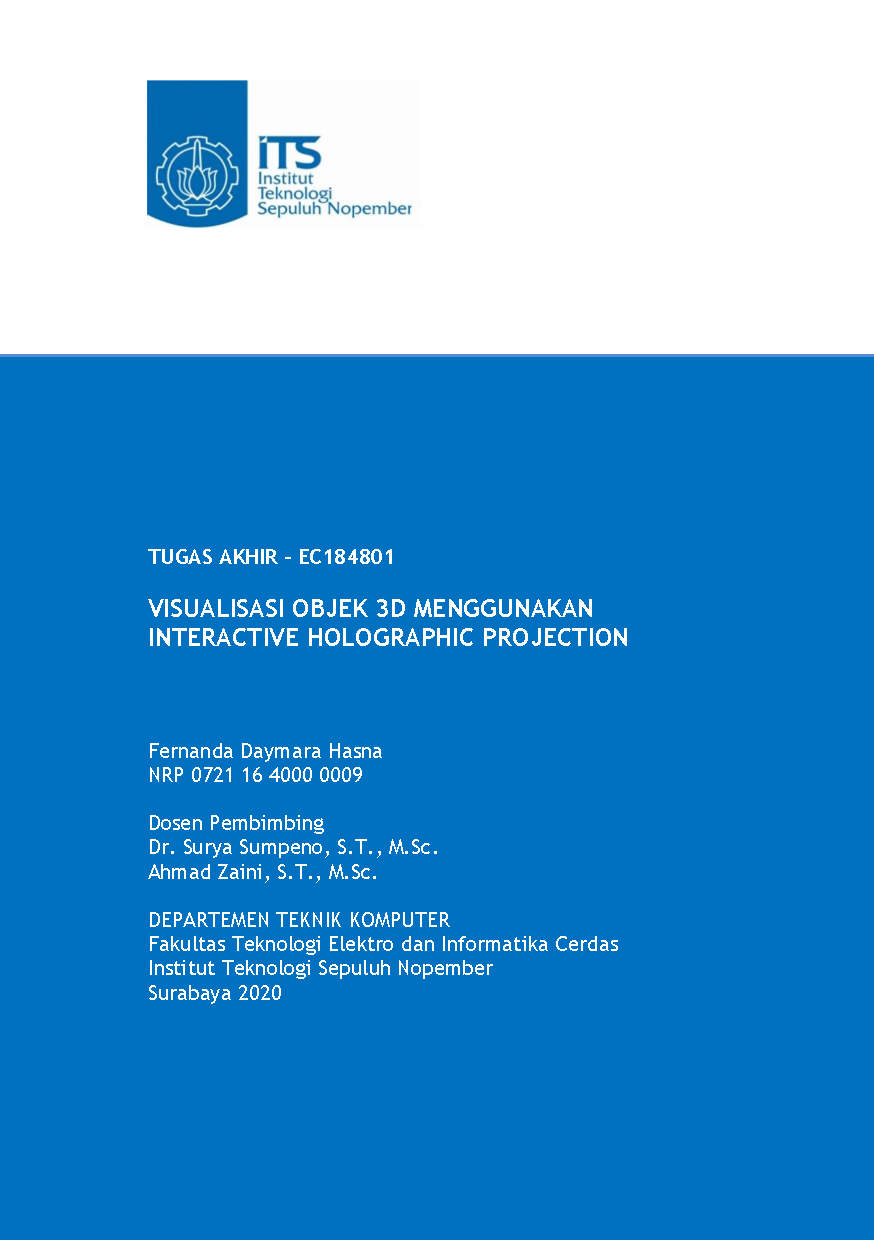
\includepdf[pages=1, offset=0 0]{ta_section/file/cover.pdf}
\bookmark[page=1, level=0]{COVER}
\cleardoublepage
\includepdf[pages=2, offset=0 0]{ta_section/file/cover.pdf}
\cleardoublepage
\includepdf[pages=3, offset=0 0]{ta_section/file/cover.pdf}
\cleardoublepage
\begin{center}
\Large\textbf{PERNYATAAN KEASLIAN\\}
\Large\textbf{TUGAS AKHIR}
\end{center}
\vspace{1ex}

\setlength{\parindent}{1cm} Dengan ini saya menyatakan bahwa isi sebagian maupun keseluruhan Tugas Akhir saya dengan judul ``\textbf{Visualisasi Objek 3D menggunakan \textit{Interactive Holographic Projection}}" adalah be-nar-benar hasil karya intelektual mandiri, diselesaikan tanpa menggunakan bahan-bahan yang tidak diijinkan dan bukan karya pihak lain yang saya akui sebagai karya sendiri.
\\

\setlength{\parindent}{1cm} Semua referensi yang dikutip maupun dirujuk telah ditulis secara lengkap pada daftar pustaka. 
\\

\setlength{\parindent}{1cm} Apabila ternyata pernyataan ini tidak benar, saya bersedia menerima sanksi sesuai peraturan yang berlaku.
\\
\\

\begin{adjustwidth}{6cm}{}
\begin{tabular}{lcp{0.65\linewidth}}
	\centering Surabaya, Juni 2020
	 & & \\
	\\
	\\
	\\
	\\
	\centering \underline{Fernanda Daymara Hasna} & & \\
	\centering NRP. 0721 16 4000 0009 & & \\ & & \\
	\end{tabular}
\end{adjustwidth}

\bookmark[page=7, level=0]{PERNYATAAN}
\cleardoublepage
\includepdf[pages=-, offset=0 0]{ta_section/file/pengesahanv2.pdf}
\bookmark[page=9, level=0]{PENGESAHAN}
\cleardoublepage


% Abstrak ID
\phantomsection
\addcontentsline{toc}{chapter}{ABSTRAK}
\begin{center}
\Large\textbf{ABSTRAK}
\end{center}
\vspace{1ex}

\begin{adjustwidth}{-0.2cm}{}
\begin{tabular}{lcp{0.6\linewidth}}
	Nama Mahasiswa &:& Fernanda Daymara Hasna \\
	Judul Tugas Akhir &:& Visualisasi Objek 3D menggunakan \textit{Interactive Holographic Projection}\\
	Dosen Pembimbing &:& 1. Dr. Surya Sumpeno, S.T., M.Sc. \\
	& & 2. Ahmad Zaini, S.T., M.Sc.  \\
\end{tabular}
\end{adjustwidth}
\vspace{1ex}

\setlength{\parindent}{0cm} Kemudahan anak-anak dalam mengakses teknologi dapat memberikan dampak negatif seperti kecanduan, pengaksesan konten yang tidak sesuai, hingga masalah kesehatan fisik dan mental\cite{sundus2018impact}. Agar manfaatnya tetap dapat dirasakan maka konten yang diakses diarahkan pada bidang edukasi, salah satunya tentang perkembangan peradaban manusia yang masih dianggap membosankan untuk dipelajari\cite{wirawan_2018}. Museum sebagai sarana dalam mempelajarinya justru tidak layak untuk dikunjungi, dimana 435 dari museum yang tercatat berada dalam kondisi yang memprihatinkan menurut Direktorat Pelestarian Cagar Budaya dan Permuseuman Kemdikbud\cite{kemendikbud_2019}. Maka dari itu, dibuatlah sistem \textit{interactive holographic projection} untuk menyampaikan informasi secara efektif dan interaktif sehingga menarik untuk dipelajari. Metode yang digunakan yaitu objek museum ditampilkan dalam bentuk hologram dan dapat digerakkan oleh pengguna menggunakan sensor pengindera tangan Leap Motion. Hasil pengujian menunjukkan bahwa gestur tangan tangan dapat memberikan respon yang bersesuaian sebesar 90.71\%, dengan 72.00\% berhasil diaktifkan menggunakan salah satu tangan dan 97.50\% menggunakan kedua tangan. Hal ini didukung dengan percobaan langsung oleh responden dengan \textit{success rate} sebesar 87.00\%. Berdasarkan kuesioner terhadap 61 responden, 47.50\% responden sangat setuju bahwa sistem ini dapat membantu pembelajaran perkembangan peradaban manusia dan 68.9\% sangat setuju bahwa sistem ini dapat mendukung perkembangan museum dan pendidikan di Indonesia.
\vspace{2ex}

Kata Kunci : Perkembangan peradaban manusia, Hologram, Interactive holographic projection.
\newpage
\cleardoublepage

% Abstract EN
\phantomsection
\addcontentsline{toc}{chapter}{\textit{ABSTRACT}}
\begin{center}
\Large\textbf{ABSTRACT}
\end{center}
\vspace{1ex}

\begin{adjustwidth}{-0.2cm}{}
\begin{tabular}{lcp{0.6\linewidth}}
	\textit{Student Name} &:& Fernanda Daymara Hasna \\
	\textit{Final Project Title} &:& \textit{3D Object Visualization using Interactive Holographic Projection} \\
	\textit{Advisors} &:& 1. Dr. Surya Sumpeno, S.T., M.Sc. \\
	& & 2. Ahmad Zaini, S.T., M.Sc.  \\
\end{tabular}
\end{adjustwidth}
\vspace{1ex}

\setlength{\parindent}{0cm} \textit{The ease of accessing technology for children may have negative impacts such as addiction, accessing inappropriate content, to physical and mental health problems\cite{sundus2018impact}. In order to make the benefits could still be felt, the content accessed is directed to the field of education, one of which is the development of human civilization which is still considered boring to study\cite{wirawan_2018}. The museum as a means of learning is actually not worth visiting, where 435 of the recorded museums are in poor condition according to the Directorate for the Preservation of Culture and Museum of the Ministry of Education and Culture\cite{kemendikbud_2019}. Therefore, an interactive holographic projection system was created to convey information effectively and interactively so that it was interesting to learn. The method used is the museum object displayed in the form of a hologram and can be moved and interacted by the user using the Leap Motion hand sensing sensor. The test results show that hand gestures can provide an appropriate response of 90.71\%, with 72.00\% successfully activated using one hand and 97.50\% using both hands. This is supported by direct experiments by respondents with success rate of 87.00\%. Based on a questionnaire of 61 respondents, 47.50\% of respondents strongly agreed that this system could help the learning of the development of human civilization and 68.9\% agreed strongly that this system could support the development of museums and education in Indonesia.}
\vspace{2ex}
	
\textit{Keywords : The development of human civilization, Hologram, Interactive holographic projection}.
\newpage

\cleardoublepage

% Kata Pengantar
\phantomsection
\addcontentsline{toc}{chapter}{KATA PENGANTAR}
\begin{center}
\Large\textbf{KATA PENGANTAR}
\end{center}

\setlength{\parindent}{1cm} Puji syukur kehadirat Tuhan Yang Maha Esa atas segala rahmat-Nya, penulis dapat menyelesaikan tugas akhir ini dengan judul \textbf{Visualisasi Objek 3D menggunakan \textit{Interactive Holographic Projection}}. Penelitian ini disusun dalam rangka memenuhi salah satu persyaratan untuk memperoleh gelar sarjana di Departemen Teknik Komputer FTEIC ITS. Keberhasilan penulis dalam pelaksanaan penelitian ini tidak lepas dari bantuan banyak pihak yang terlibat. Oleh karena itu, penulis mengucapkan terima kasih kepada :
\vspace{1ex}

\begin{enumerate}[nolistsep]
  \item Kedua orang tua, beserta keluarga, dan saudara-saudari tercinta yang selalu memberikan dukungan baik secara moral maupun material selama pelaksanaan penelitian ini.
  \item Bapak Dr. Supeno Mardi Susiki Nugroho, S.T., M.T. selaku Kepala Departemen Teknik Komputer FTEIC-ITS.
  \item Bapak Dr. Surya Sumpeno, S.T., M.Sc. dan bapak Ahmad Zaini, S.T., M.Sc. selaku dosen pembimbing, atas dukungan dan bimbingan selama pengerjaan penelitian ini.  
  \item Bapak Dr. I Ketut Eddy Purnama, S.T.,M.T. selaku dosen wali, atas dukungan non teknis selama pengerjaan penelitian ini.
  \item Bapak-ibu dosen pengajar serta staff Departemen Teknik Komputer, atas pengajaran, bimbingan, serta perhatian yang diberikan kepada penulis selama ini.
  \item Seluruh teman-teman dari Teknik Komputer dan juga angakatan e56.
\end{enumerate}
\vspace{1ex}

Penulis menyadari bahwa dalam penyusunan buku hasil penelitian ini jauh dari kata sempurna, untuk itu penulis memohon kritik dan saran yang membangun sehingga  dapat menjadi lebih baik lagi. Harapannya penelitian ini dapat berguna sebagai acuan penelitian-penelitian selanjutnya dan bermanfaat bagi kita semua. Aamiin.
\begin{flushright}
\begin{tabular}[b]{c}
  Surabaya, Juni 2020
  \\
  \\
  \\
  Penulis
\end{tabular}
\end{flushright}
\cleardoublepage

% Daftar Isi
\phantomsection
\renewcommand*\contentsname{DAFTAR ISI}
\addcontentsline{toc}{chapter}{\contentsname}
\titlespacing*{\chapter}{0pt}{-4ex}{2ex}
\tableofcontents	
\cleardoublepage

% Daftar Gambar
\phantomsection
\renewcommand*\listfigurename{DAFTAR GAMBAR}
\addcontentsline{toc}{chapter}{\listfigurename}
\titlespacing*{\chapter}{0pt}{-4ex}{2ex}
\listoffigures
\cleardoublepage

% Daftar Tabel
\phantomsection
\renewcommand*\listtablename{DAFTAR TABEL}
\addcontentsline{toc}{chapter}{\listtablename}
\titlespacing*{\chapter}{0pt}{-4ex}{2ex}
\listoftables
\cleardoublepage

% Nomenklatur
%\addcontentsline{toc}{chapter}{NOMENKLATUR}
%\begin{center}
	\Large\textbf{NOMENKLATUR}
\end{center}
\vspace{1ex}

\begin{tabular}{c m{30em}}
	$ah$	& : Nilai getaran horizontal (g)\\
	$av$	& : Nilai getaran vertikal (g) \\
	$V_{act}$ & : Kecepatan aktual (km/jam) \\
	$V_{max}$ & : Kecepatan maksimal (km/jam) \\
	$N$ & : Nilai indeks jalur\\
	$N_{x}$ & : Nilai indeks jalur horizontal \\
	$N_{y}$ & : Nilai indeks jalur vertikal \\
	$A_{off}$ & : \textit{Offset error} dari sensor akselerometer (g) \\
	$A_{out}$ & : Nilai sensor akselerometer sebelum kalibrasi (g) \\
	$A_{act}$ & : Nilai sensor akselerometer setelah kalibrasi (g) \\
	$Gn$ & : Gain dari sensor akselerometer (g) \\
	$A_{g+}$ & : Nilai sensor akselerometer ketika posisi positif (g) \\
	$A_{g-}$ & : Nilai sensor akselerometer ketika posisi negatif (g) \\
	
\end{tabular}
\vspace{1ex}
%\cleardoublepage


% BAB isi buku
\titleformat{\chapter}[display]{\bfseries\Large}{BAB \centering\thechapter}{0ex}{\vspace{0ex}\centering}[\vspace{0ex}]
\titleformat{\section}{\bfseries\large}{\MakeUppercase{\thesection}}{1ex}{}
\titleformat{\subsection}{\bfseries\large}{\MakeUppercase{\thesubsection}}{1ex}{}
\titleformat{\subsubsection}{\bfseries\large}{\MakeUppercase{\thesubsubsection}}{1ex}{}
\titlespacing*{\chapter}{0pt}{-4ex}{0pt}
\titlespacing{\section}{0pt}{0pt}{0pt}
\titlespacing{\subsection}{0pt}{0pt}{0pt}
\titlespacing{\subsubsection}{0pt}{0pt}{0pt}

% Indent Paragraph
\setlength{\parindent}{0.8cm}

% Penambahan halaman kosong otomatis
\chapter{PENDAHULUAN}
\pagenumbering{arabic}
\vspace{4ex}

\hspace{\parindent} Penelitian ini di latar belakangi oleh berbagai kondisi yang menjadi acuan. Selain itu juga terdapat beberapa permasalahan yang akan dijawab sebagai luaran dari penelitian.
\vspace{2ex}

\section{Latar Belakang}
\vspace{1ex}
	Kemajuan teknologi dan internet memberikan kemudahan akses terhadap segala macam konten dan manfaat untuk kehidupan sehari-hari, tak terkecuali bagi anak-anak. Sudah dikenalkan sejak dini ini memudahkan anak-anak dalam beradaptasi dan terbiasa berinteraksi dengan \textit{gadget}. Hal ini dapat menyebabkan dampak negatif seperti mengetahui informasi yang belum pantas diketahui, kecanduan terhadap gadget, hingga menimbulkan efek terhadap kesehatan fisik dan mental\cite{sundus2018impact}. Sedangkan mereka tidak mengerti apakah informasi yang diterimanya itu baik atau buruk terhadap dirinya, sehingga orang dewasa lah yang berperan dalam menentukan informasi dan konten apa saja yang dibutuhkan dan pantas untuk diterima anak-anak. Dalam hal ini, penggunaan teknologi dapat memberikan dampak positif selama informasi yang disajikan sesuai untuk diterima oleh anak-anak. Informasi yang cocok dan layak untuk diakses anak-anak adalah mengenai edukasi, salah satunya adalah perkembangan peradaban manusia. 
	
	Konten bidang sejarah ini perlu dikenalkan pada anak-anak karena mempelajari sejarah dapat meningkatkan kemampuan berpikir kritis dan mengolah informasi. Presepsi sosial yang tersebar di masyarakat yang menyebabkan kurangnya minat untuk mempelajarinya dikarenakan sejarah sendiri sering dianggap sebagai pelajaran menghafal yang terkesan membosankan\cite{wirawan_2018}. Salah satu metode yang dapat mendukung pembelajaran sejarah adalah melalui kunjungan ke museum terkait. Namun berdasarkan penuturan Direktur Pelestarian Cagar Budaya dan Permuseuman Kementerian Pendidikan dan Kebudayaan (Kemendikbud) Firda Arda Ambas, hampir dari serempat dari 435 museum yang tercatat kondisinya memprihatinkan bahkan termasuk ke dalam kategori tidak layak untuk menyimpan koleksi sejarah dan jarang dikunjungi masyarakat\cite{kemendikbud_2019}. Koleksi sejarah hanya disimpan dan dipajang saja, terkadang kurang terawat sehingga kondisinya mulai rusak dan terkesan kumuh (tidak bagus). Mengunjungi museum dipandang sebagai kegiatan membosankan, sebatas untuk melihat barang-barang yang monoton tanpa adanya suatu hal yang dapat meningkatkan rasa penasaran pengunjung. Padahal sudah seharusnya dan selayaknya fasilitas utama dan pendukung yang disediakan selalu dikembangkan karena media penyampaian informasi yang menarik akan lebih mudah dipahami dan menyenangkan bagi pengunjung (meningkatkan \textit{visitor experience})\cite{sheng2012study}. 
\vspace{2ex} 
 
\section{Permasalahan}
\vspace{1ex}
	Berdasarkan latar belakang yang telah dijelaskan, media informasi berbasis teknologi digital terkait perkembangan peradaban manusia di museum di Indonesia tidak banyak diaplikasikan dan tidak interaktif. Hal ini menyebabkan informasi yang disampaikan kurang maksimal sehingga dibutuhkan sebuah media yang dapat menyampaikan informasi secara efektif dan interaktif.
\vspace{2ex}

\section{Tujuan}
\vspace{1ex}
	Tujuan dari Tugas Akhir ini adalah memberikan alternatif media pembelajaran bidang sejarah perkembangan peradaban manusia dengan memanfaatkan \textit{hologram projector} yang dapat dikontrol oleh \textit{user} sehingga informasi yang disampaikan dapat dipahami lebih mudah dan menyenangkan.
\vspace{2ex}

\section{Batasan Masalah}
\vspace{1ex}
	Untuk memfokuskan permasalahan yang diangkat maka dilakukan pembatasan masalah. Batasan-batasan masalah tersebut diantaranya adalah :
	\vspace{0.5ex}
	\begin{enumerate} [nolistsep]
		\item Dimensi set dan komponen utama yang terdiri dari Leap Motion Controller, Monitor, dan \textit{Pyramid Hologram}.
		\vspace{0.5ex}
		
		\item Objek yang divisualisasikan berupa benda peninggalan perkembangan peradaban manusia  yang diwakilkan dalam zona purbakala, klasik (Hindu-Buddha), kolonial dan pergerakan kemerdekaan serta IPTEK (Ilmu Pengetahuan dan Teknologi).
		\vspace{0.5ex}
				
		\item Fitur yang disajikan berupa gestur untuk mengeksplorasi objek hologram selayaknya di dunia nyata, seperti memutar dan mengubah ukuran objek.
		\vspace{0.5ex}
	\end{enumerate}
	\vspace{2ex}

\section{Sistematika Penulisan}
\vspace{1ex}
	Laporan penelitian tugas akhir ini tersusun dalam sistematika dan terstruktur sehingga mudah dipahami dan dipelajari oleh pembaca maupun seseorang yang ingin melanjutkan perancangan sistem. Sistematika penulisan laporan Tugas Akhir ini yaitu:
	\vspace{0.5ex}
	\begin{enumerate}[nolistsep]
		\item BAB 1 Pendahuluan
		
		Bab I berisi uraian tentang latar belakang, permasalahan, tujuan, batasan masalah, metodologi, dan sistematika penulisan dari penelitian tugas akhir ini.
		\vspace{0.5ex}
	
		\item BAB 2 Tinjauan Pustaka
	
		Bab II berisi tentang uraian secara sistematika teoriteori yang berhubungan dengan permasalahan yang dibahas pada penelitian ini. Teori-teori ini digunakan sebagai dasar dalam penelitian, yaitu teori \textit{Holographic Projection}, perangkat \textit{Leap Motion} dan teori penunjang lain termasuk \textit{datasheet} spesifikasi setiap komponen lain yang membangun sistem.
		\vspace{0.5ex}
	
		\item BAB 3 Perancangan Sistem dan Implementasi
	
		Bab III berisi tentang rancangan pemecahanan masalah beserta implementasinya. Berisikan mengenai perencanaan rancangan, uraian rinci mengenai metodologi yang digunakan, dan pemaparan hasil implementasi sistem yang dilakukan. 
		\vspace{0.5ex}
	
		\item BAB 4 Pengujian dan Analisis
	
		Bab IV berisi tentang pengujian eksperimen yang telah dilakukan terhadap sistem dan parameter yang terlibat. Selain itu, bab ini juga memuat hasil dan analisis dari uji coba yang dilakukan pada Tugas Akhir ini.
		\vspace{0.5ex}
		
		\item BAB 5 Penutup
		
		BAB V berisi tentang kesimpulan yang diambil berdasarkan penelitian dan pengujian yang telah dilakukan. Saran dan kritik yang membangun untuk pengembangan lebih lanjut juga dituliskan pada bab ini.
		\vspace{0.5ex}
	\end{enumerate}
\vspace{2ex}

\begin{comment}
\section{Relevansi}
\vspace{1ex}
	Penelitian Tugas Akhir ini mengenai \colorbox{yellow}{cari tau ini tentang apa isinya, kalau dari PedomanTA isinya Manfaat TA}
\vspace{2ex}
\end{comment}
\cleardoublepage
\chapter{TINJAUAN PUSTAKA}
\vspace{4ex}

\hspace{\parindent} Demi mendukung penelitian ini, dibutuhkan beberapa teori penunjang sebagai bahan acuan dan referensi. Pada bagian ini, teori penunjang tersebut dijabarkan secara ringkas untuk menjadi dasar dalam menyelesaikan penelitian yang lebih terarah.
\vspace{2ex}

\section{\textit{Related Researches}}
\vspace{1ex}
	Pada sub bab ini dijelaskan mengenai beberapa penelitian sebelumnya yang berelasi dengan tugas akhir ini.
\vspace{1.5ex}
	
	\subsection{Proyeksi Interaktif Objek Hologram 3D menggunakan \textit{Aerial Projection}}
	\vspace{1ex}
		Penelitian ini mencoba konsep dan desain dari sistem \textit{interactive aerial projection} yang dilakukan dengan \textit{prototype demonstration}. Penelitian ini berfokus untuk menampilkan objek 3D di udara dan manipulasi objek 3D dari \textit{finger movement}. Sistem yang berhasil dibuat pada penelitian ini terdiri dari \textit{Reconstruction of 3D Object} dengan menggunakan \textit{pyramid hologram device}, \textit{Projection of 3D Hologram Object in the Mid-Air} dengan \textit{concave mirror} berbentuk parabola, dan \textit{Interactive Manipulation of 3D Hologram Object} dengan \textit{leap motion}. Sistem ini berhasil dibangun meskipun dengan \textit{workspace} dan interaksi yang terbatas.\cite{mahfud2016interactive}
	\vspace{1.5ex}

	\subsection{Pembuatan Dataset \textit{Hand Gesture} menggunakan \textit{Leap Motion}}
	\vspace{1ex}
		Penelitian ini berkaitan dengan \textit{3D dynamic gesture recognition} berdasarkan posisi ujung jari dan telapak 	tangan. Penelitian ini berfokus pada proses pembuatan dataset baru yang digunakan dalam penyusunan sebuah sistem kontrol. Dataset yang dibuat berpedoman dari \textit{general commands} (yang umum diterapkan pada \textit{leap motion}) sebagai parameter \textit{training}. Metode ini berhasil diterapkan dengan nilai akurasi yang cukup tinggi, sehingga dapat diterapkan untuk mengembangkan \textit{feature} baru.\cite{ameur2016comprehensive}
	\vspace{1.5ex}
	
	\subsection{Faktor-faktor yang Mempengaruhi \textit{Interactive 3D Holographic Projection System} untuk \textit{Experiential Learning}}
	\vspace{1ex}
		Penelitian ini berkaitan dengan informasi yang dapat disajikan dalam mendukung \textit{interactive ecperiental learning} yang menghasilkan pedoman untuk \textit{3D display and control of interactive experience}. Faktor-faktor tersebut dinyatakan dalam tabel \ref{tab:faktor-nilaiguna-3d}.
		\vspace{-2ex}
		\begin{table}[!htb]
			\caption{Faktor-faktor yang Memengaruhi Nilai Guna \textit{3D Holographic Projection System}}
			\label{tab:faktor-nilaiguna-3d}
			\vspace{-2ex}
			\begin{center}
			\begin{tabular}{|C{0.4cm}|L{2.2cm}|L{6.3cm}|}
				\hline
				\textbf{No} & \multicolumn{1}{c|}{\textbf{Item}} & \multicolumn{1}{c|}{\textbf{Deskripsi}}\\ \hline
				1.& \textit{Image Space}               & Ukuran dari  objek pada \textit{holographic projection}                             \\ \hline
				2.& \textit{Icon Shape}                & Bentuk dan ukuran simbol penyusun \textit{interface}                                 \\ \hline
				3.& \textit{Cursor Reminder}           & Efek pergerakan kursor pada \textit{interface}                                       \\ \hline
				4.& \textit{Rich Contents}             & Kompleksitas informasi dari \textit{learning objective} yang ingin disampaikan \\ \hline
				5.& \textit{Level Guider}              & Kesesuaian \textit{interface}  dengan scene yang sedang berjalan                          \\ \hline
				6.& \textit{Compatible Gestures}       & Sensitivitas dan kesesuaian respons terhadap \textit{gesture} yang diberikan               \\ \hline
				7.& \textit{Sensitive Cursors}         & Sensitivitas dari pergerakan kursor terhadap \textit{interface}                           \\ \hline
				8.& \textit{Adjustable Function}       & Kemampuan \textit{user} dalam mengatur \textit{control function}                          \\ \hline
				9.& \textit{Sound Feedback}            & \textit{Feedback} dari \textit{interface} saat ada instruksi maupun \textit{click sound}  \\ \hline
				10.& \textit{Background Music (BGM)}    & Musik atau lagu yang diputar saat suatu \textit{scene} sedang berlangsung                 \\ \hline
				11.& \textit{Switching Effect}          & Efek \textit{visual animation} saat perpindahan \textit{scene}                            \\ \hline
				12.& \textit{Ambient Brightness}        & Tingkat kecerahan \textit{environment} sekitar saat \textit{holographic projection }      \\ \hline
			\end{tabular}
			\end{center}
		\end{table}
	\vspace{2ex}
	
	Penelitian ini menghasilkan kesimpulan bahwa faktor-faktor ini dapat membantu penyampaian informasi lebih efektif dan efisien. Sistem \textit{3D holographic projection interactive} ini dapat memberikan output yang berbeda dibandingkan dengan pembelajaran konvensional dengan dengan buku. Penelitian ini pun juga mengemukakan bahwa hasil dari penelitian ini dapat diterapkan pada pembelajaran digital seperti \textit{virtual museum exhibition}.\cite{huang2018factors}
\vspace{2ex}

\section{Visualisasi Objek 3D}
\vspace{1ex}
	Visualisasi adalah suatu metode rekayasa dalam menampilkan sebuah informasi, baik gambar, diagram, ataupun animasi. Dalam memvisualisasikan objek 3D (selanjutnya disebut model 3D), yang perlu diperhatikan adalah bagaimana objek tersebut berhasil merepresentasikan objek di dunia nyata. Suatu model 3D tidak menjamin dapat memberikan ilusi mirip dengan objek aslinya yang dilihat dengan penginderaan manusia (\textit{real world}). Pada dasarnya, model 3D merupakan hasil pemrosesan dan pemberian efek cahaya terhadap bentuk 2D sehingga objek tersebut seolah-olah memiliki kedalaman (sumbu x, y, dan z). Pencahayaan ini mempengaruhi realsitas suatu model 3D. Tanpa adanya pencahayaan, model 3D tidak memiliki bayangan dan terlihat tidak memiliki kedalaman. 
	\begin{comment}
		Perbandingan model 3D yang diberikan pencahayaan maupun tidak ditunjukkan pada gambar \ref{fig:model3d_cahaya}.
	\begin{figure} [H]
	\includegraphics[scale=0.4]{img/bab2/model3d_cahaya.png}
	\caption{Perbandingan efek pencahayaan pada model 3D. \colorbox{yellow}{model awal > model dgn pencahayaan diubah2 posisinya}}
	\label{fig:model3d_cahaya}
	\end{figure}
	\end{comment}
			
	Selain pencahayaan, efek dan detail yang diberikan pada permukaan objek juga membedakan realistas antar model 3D. \textit{Texturing} berfungsi membuat sebuah objek menjadi lebih nyata seperti aslinya dengan memberikan karakteristik terhadap permukaan objek. Objek nyata tidak selalu memiliki permukaan yang halus atau rata, maka untuk menampilkan detail permukaan pada model 3D dibutuhkan \textit{UV map}. \textit{UV map} digunakan untuk menekankan bentuk detail objek dimana mencakup pengaturan bayangan, pewarnaan, dan bentuk teksturnya sehingga dapat memberikan efek realistis pada model 3D tanpa harus dimodelkan bentuknya karena \textit{uv mapping} adalah proses 'penempelan' 2D image terhadap permukaan model 3D. Tingkat detail model 3D disesuaikan dengan peruntukannya karena semakin detail modelnya, maka dibutuhkan \textit{hardware} dengan spesifikasi yang lebih canggih agar program tersebut dapat berjalan dengan baik. Contoh dari objek sebelum dan setelah \textit{uv mapping} ditunjukkan pada gambar \ref{fig:model3d_tekstur}.
	\begin{figure} [H]
		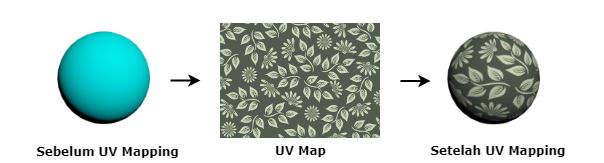
\includegraphics[scale=0.5]{img/bab2/model3d_tekstur.png}
		\caption{Objek sebelum dan setelah\textit{uv mapping}\cite{uvmap}.}
		\label{fig:model3d_tekstur}
	\end{figure}
\vspace{2ex}
	
\section{Proyeksi Hologram}
\vspace{1ex}
	Holografi (\textit{holography}), berasal dari bahasa Yunani "\textit{Holos}" berarti seluruh dan "\textit{Graphe} berarti tulisan, adalah sebuah metode yang merekam cahaya yang tersebar dan merekonstruksi pola cahaya tersebut seolah-olah membentuk suatu objek \cite{akshay_2015}. Objek yang memiliki lebar (\textit{width}), ketinggian (\textit{height}) dan kedalaman (\textit{depth}) ini dikenal sebagai objek tiga dimensi. Objek yang dihasilkan holografi dikenal sebagai hologram, yaitu objek atau \textit{image} yang dibentuk berdasarkan penyebaran/pembelokan (difraksi) pancaran cahaya. Cahaya yang dikeluarkan oleh proyektor atau alat pemancar lain akan dibelokkan dan berinterferensi dengan cahaya lain yang saling menguatkan dan membentuk pola yang dapat dilihat. Teknologi hologram yang sederhana mengadopsi teknik \textit{Pepper’s Ghost Illusion} oleh John Henry Pepper (1821-1900). \textit{Pepper’s Ghost Illusion} adalah teknik yang diterapkan pada teater untuk memberikan efek objek yang tidak nyata seperti transparan layaknya hantu. Objek transparan ini dihasilkan dari objek atau aktor yang terletak di \textit{blind spot} penonton, dimana akan dipancarkan cahaya dan dipantulkan melalui sebuah kaca yang dipasang 45° di depan penonton. Sehingga hasil pemantulannya dimanfaatkan sebagai ‘aktor’ hantu yang dilihat oleh penonton dan memainkan peran sesuai cerita\cite{vishnu2017hologram}.
	
	Hologram terbentuk karena adanya interferensi (interaksi tumpang tindih pada suatu titik tertentu) atau penggabungan cahaya antara \textit{reference beam} dan \textit{object beam}. Sinar laser mengarah ke \textit{beam splitter} terbagi menjadi dua \textit{reference beam} \cite{akshay_2015}. Salah satunya diteruskan ke objek terkait menjadi \textit{object beam}. Keduanya (\textit{reference beam} dan \textit{object beam}) jatuh pada di sebuah medium dan memunculkan bentuk hologram dari objek tersebut. Jika ada cahaya lain yang koheren dengan laser, maka cahaya ini dapat memengaruhi objek hologram yang dibentuk. Sehingga perlu meminimalisir adanya cahaya lain yang dapat mengganggu. Ilustrasi terbentuknya hologram ditampilkan pada gambar \ref{fig:hologram_kerja}.
	\begin{figure} [H]
		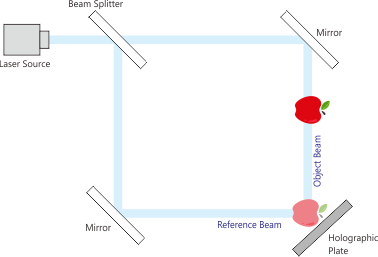
\includegraphics[scale=0.4]{img/bab2/hologram_kerja.png}
		\caption{Cara kerja hologram.}
		\label{fig:hologram_kerja}
	\end{figure}
	
	Hal yang dibutuhkan untuk menciptakan bentuk hologram adalah metode bagaimana objek asli tersebut dapat direkonstruksi dalam bentuk hologram, salah satu media yang banyak digunakan adalah \textit{pyramid hologram}. \textit{Pyramid hologram} adalah potongan media tembus pandang yang disusun dalam bentuk piramida dimana dapat memantulkan objek asli pada sebuah titik. Setiap sisi piramida memantulkan (refleksi) objek yang ditampilkan pada  monitor yang terletak di bawahnya, sehingga semua hasil pemantulan menyebabkan ojek 3D dapat dilihat dari setiap sisi. Hasil yang diberikan pun  menciptakan ilusi objek 3D yang muncul di udara, tepatnya di sisi bagian dalam piramida tersebut. Faktor ini menyebabkan besarnya objek hologram yang dihasilkan tergantung dari besarnya piramida dan monitor yang digunakan. Pemilihan jenis dan ketebalan bahan piramida dapat menentukan bentuk hologram yang dibangun. Semakin tebal bahannya, maka semakin buram (blur) objek hologram yang didapat dikarenakan adanya pemantulan berulang\cite{hologrampyramid}. Beberapa \textit{pyramid hologram} yang banyak digunakan adalah piramida 1 sisi, 3 sisi, dan 4 sisi. Berbeda jenis piramid yang digunakan maka \textit{hologram video} yang diputar pun berbeda-beda, dimana objek asli harus menghadap sisi piramida\cite{mahfud2016interactive}. Ketiganya memiliki kelebihan dan kekurangannya masing-masing.
	
	\subsection{Piramida 1 Sisi}
	\vspace{1ex}
	\textit{Pyramid hologram} 1 sisi adalah yang paling sederhana. Hanya dapat memantulkan dari 1 sisi menyebabkan objek hologram yang dihasilkan memiliki ukuran yang paling besar di antar jenis-jenis yang lain. Sama seperti pada \textit{Pepper’s Ghost Illusion}, objek asli yang ditampilkan pada monitor diletakkan pada salah satu sisi piramida membentuk sudut 45° dan hasil hologramnya muncul seolah-olah berada di luar piramida. Bentuk \textit{hologram video} yang diputar pun hanya menampilkan 1 objek yang diposisikan di tengah monitor dan hasil yang diperoleh seperti gambar \ref{fig:piramid1}.
	\begin{figure} [H]
		\subfloat[Bentuk piramida 1 sisi\cite{fotop1}.]{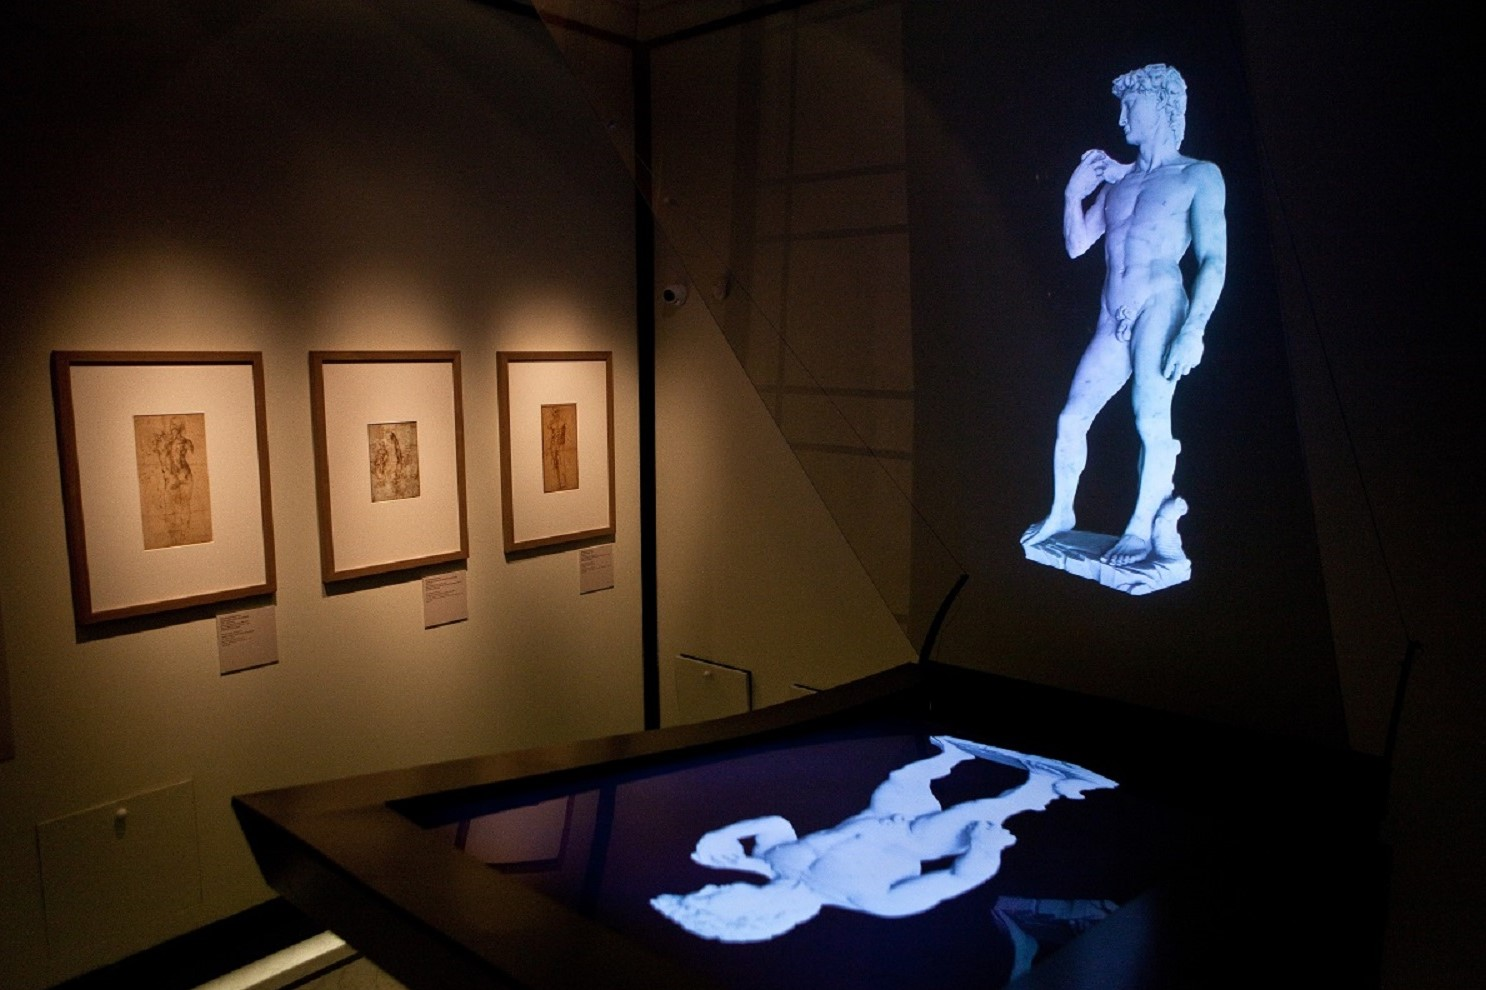
\includegraphics[width=0.47\textwidth]{img/bab2/p1_foto.jpg}}
		\hspace{0.1em}
		\subfloat[Video untuk piramida 1 sisi\cite{videop1}.]{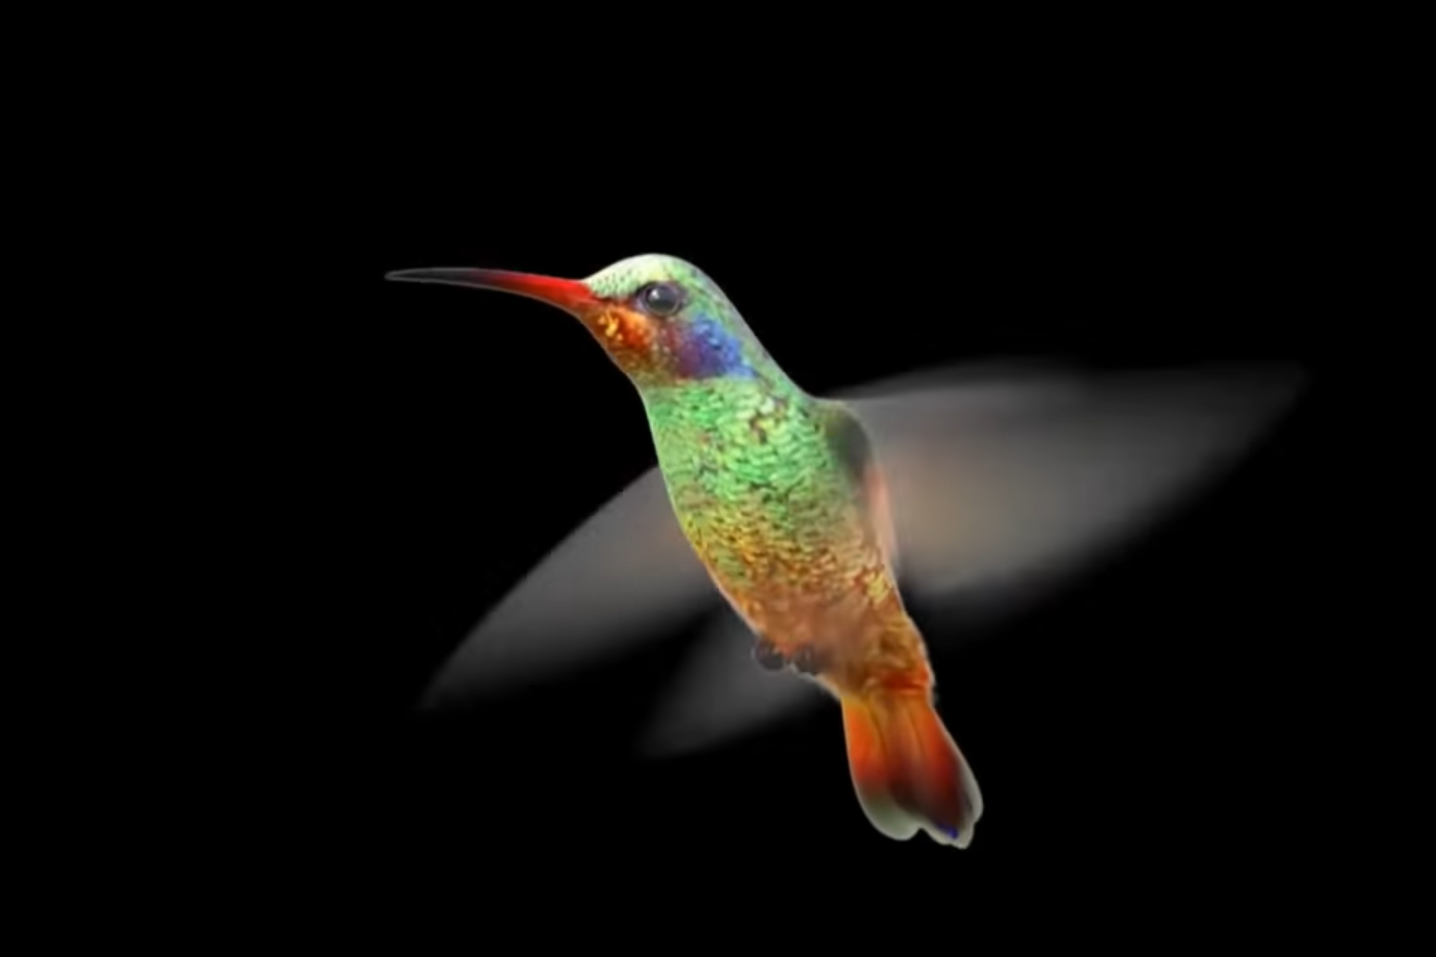
\includegraphics[width=0.47\textwidth]{img/bab2/p1_video.png}}
		\caption{Piramida 1 sisi}
		\label{fig:piramid1}
	\end{figure}
	\vspace{1.5ex}
	
	\subsection{Piramida 3 Sisi}
	\vspace{1ex}
	\textit{Pyramid hologram} 3 sisi adalah 'setengah' dari piramida 4 sisi. Piramida jenis ini memungkinkan objek hologram dapat dilihat dari 3 sisi sejauh 270° dengan salah satu sisinya tertutup, sehingga banyak diaplikasikan untuk memberikan animasi pada objek koleksi yang dipajang\cite{ironman}. Berbeda dengan kedua jenis yang lain, kebanyakan piramida jenis ini digunakan untuk memutar \textit{hologram video} dengan posisi monitor yang menghadap ke bawah. Bentuk \textit{hologram video} yang diputar memiliki 3 objek yang membentuk huruf Y (antar objek membentuk sudut sebesar 60°) dan hasil yang diperoleh seperti gambar \ref{fig:piramid3}. Menampilkan 3 objek dalam 1 monitor menyebabkan objek hologram yang ditampilkan tidak sebesar pada piramid 1 sisi.
	\begin{figure} [H]
		\subfloat[Bentuk piramida 3 sisi\cite{fotop3}.]{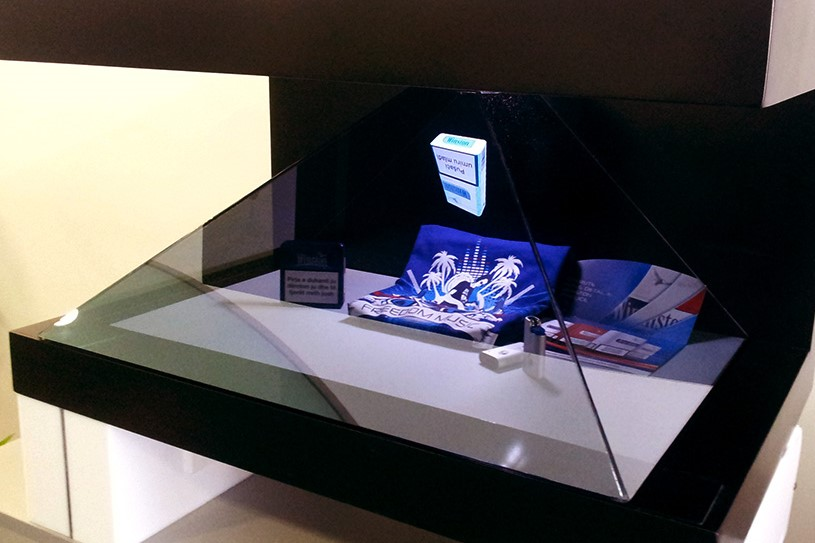
\includegraphics[width=0.47\textwidth]{img/bab2/p3_foto.jpg}}
		\hspace{0.1em}
		\subfloat[Video untuk piramida 3 sisi\cite{videop3}.]{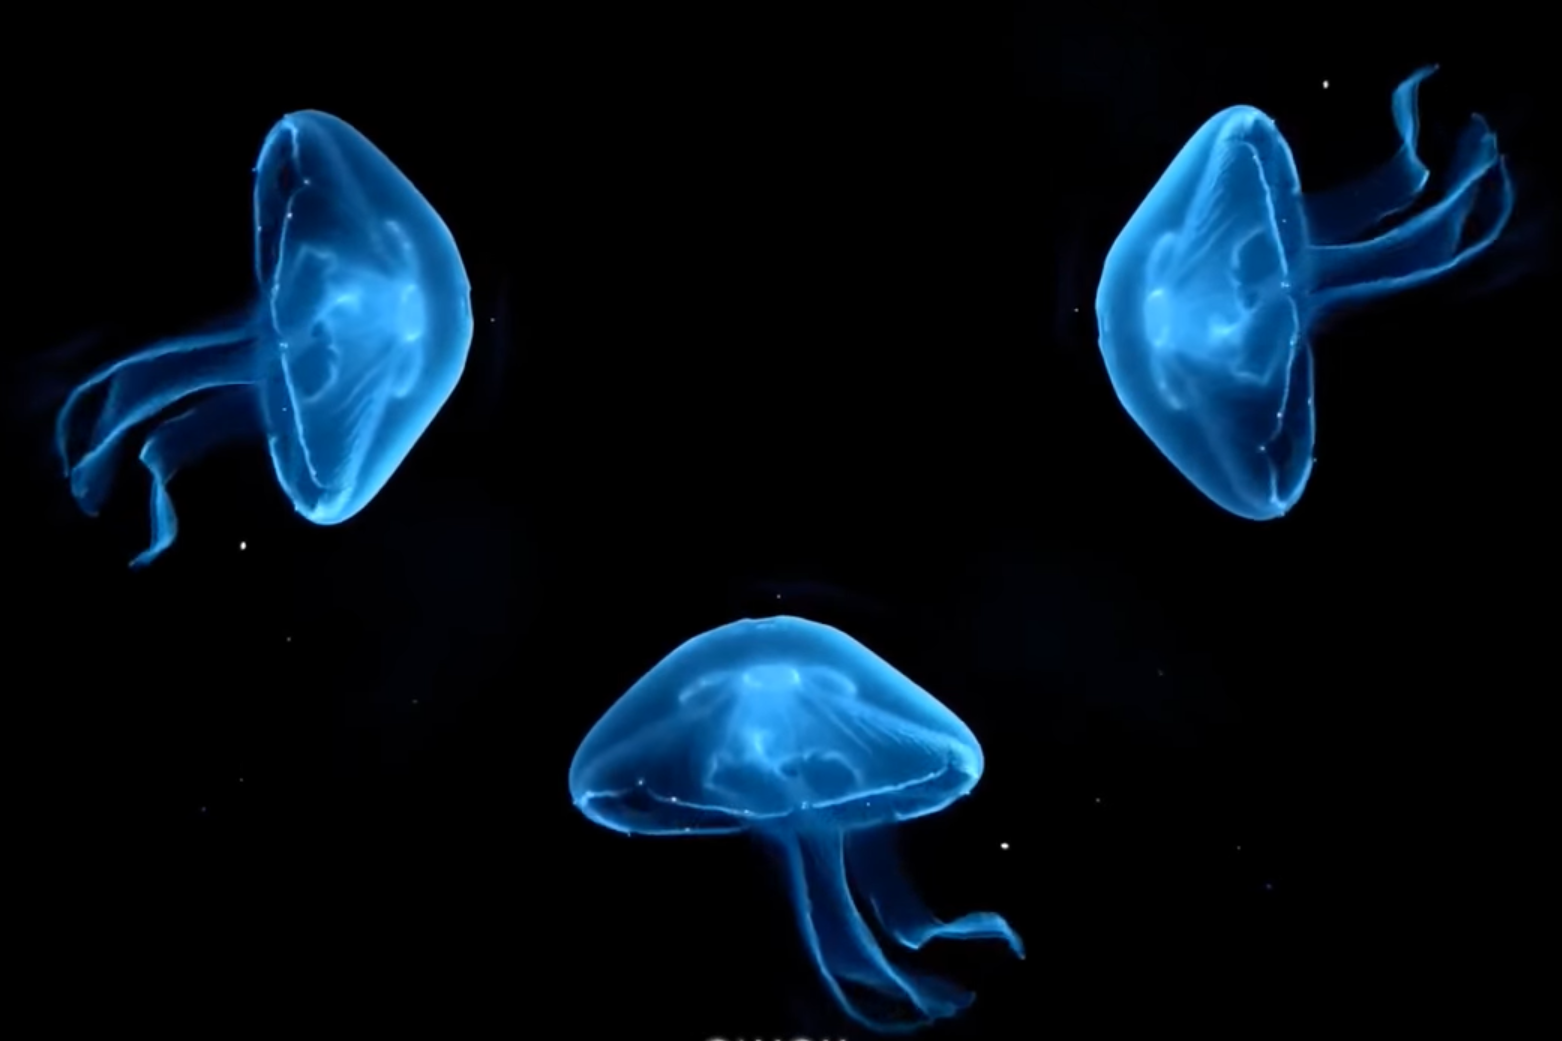
\includegraphics[width=0.47\textwidth]{img/bab2/p3_video.png}}
		\caption{Piramida 3 sisi}
		\label{fig:piramid3}
	\end{figure}
	\vspace{1.5ex}
	
	\subsection{Piramida 4 Sisi}
	\vspace{1ex}
	\textit{Pyramid hologram} 3 sisi adalah jenis piramida yang paling umum dikenal. Karena ke empat sisi yang simetris (6 : 3.5 : 1), piramida jenis ini banyak dibuat dengan bahan yang mudah dan dimanfaatkan untuk memutar \textit{hologram video} pada \textit{smartphone}\cite{tutorialpiramid}. Piramida 4 sisi ini dapat digunakan untuk memutar \textit{hologram video} dengan monitor menghadap ke atas maupun menghadap ke bawah.	Bentuk \textit{hologram video} yang diputar memiliki 4 objek yang membentuk tanda tambah (+) (antar objek membentuk sudut sebesar 90°) dan hasil yang diperoleh seperti gambar \ref{fig:piramid4}. Menampilkan 4 objek dalam 1 monitor menyebabkan objek hologram yang ditampilkan tidak sebesar pada kedua jenis lainnya, namun dapat dilihat dari segala arah (360°).
	\begin{figure} [H]
		\subfloat[Bentuk piramida 4 sisi\cite{fotop4}.]{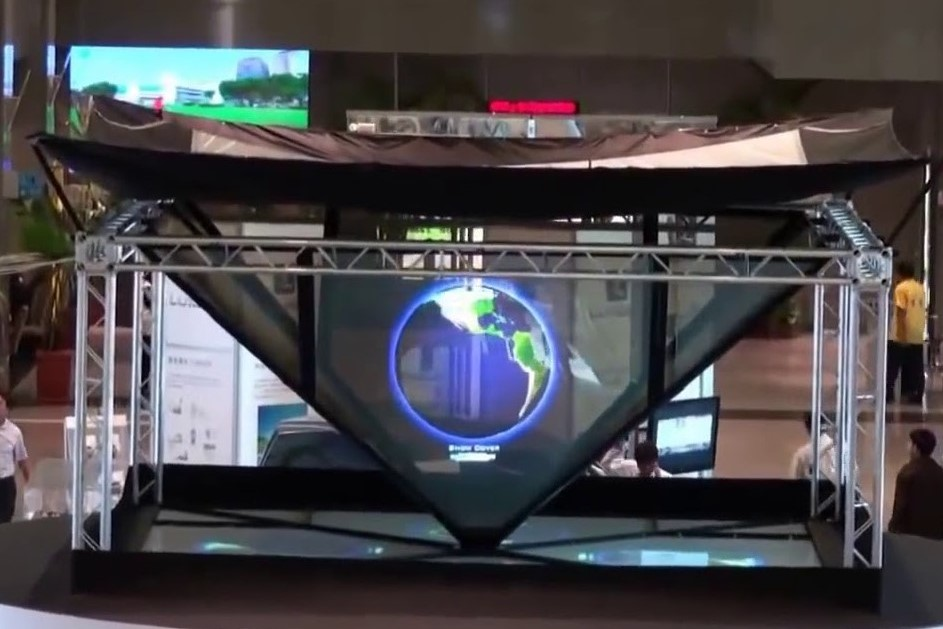
\includegraphics[width=0.47\textwidth]{img/bab2/p4_foto.jpg}}
		\hspace{0.1em}
		\subfloat[Video untuk piramida 4 sisi\cite{videop4}.]{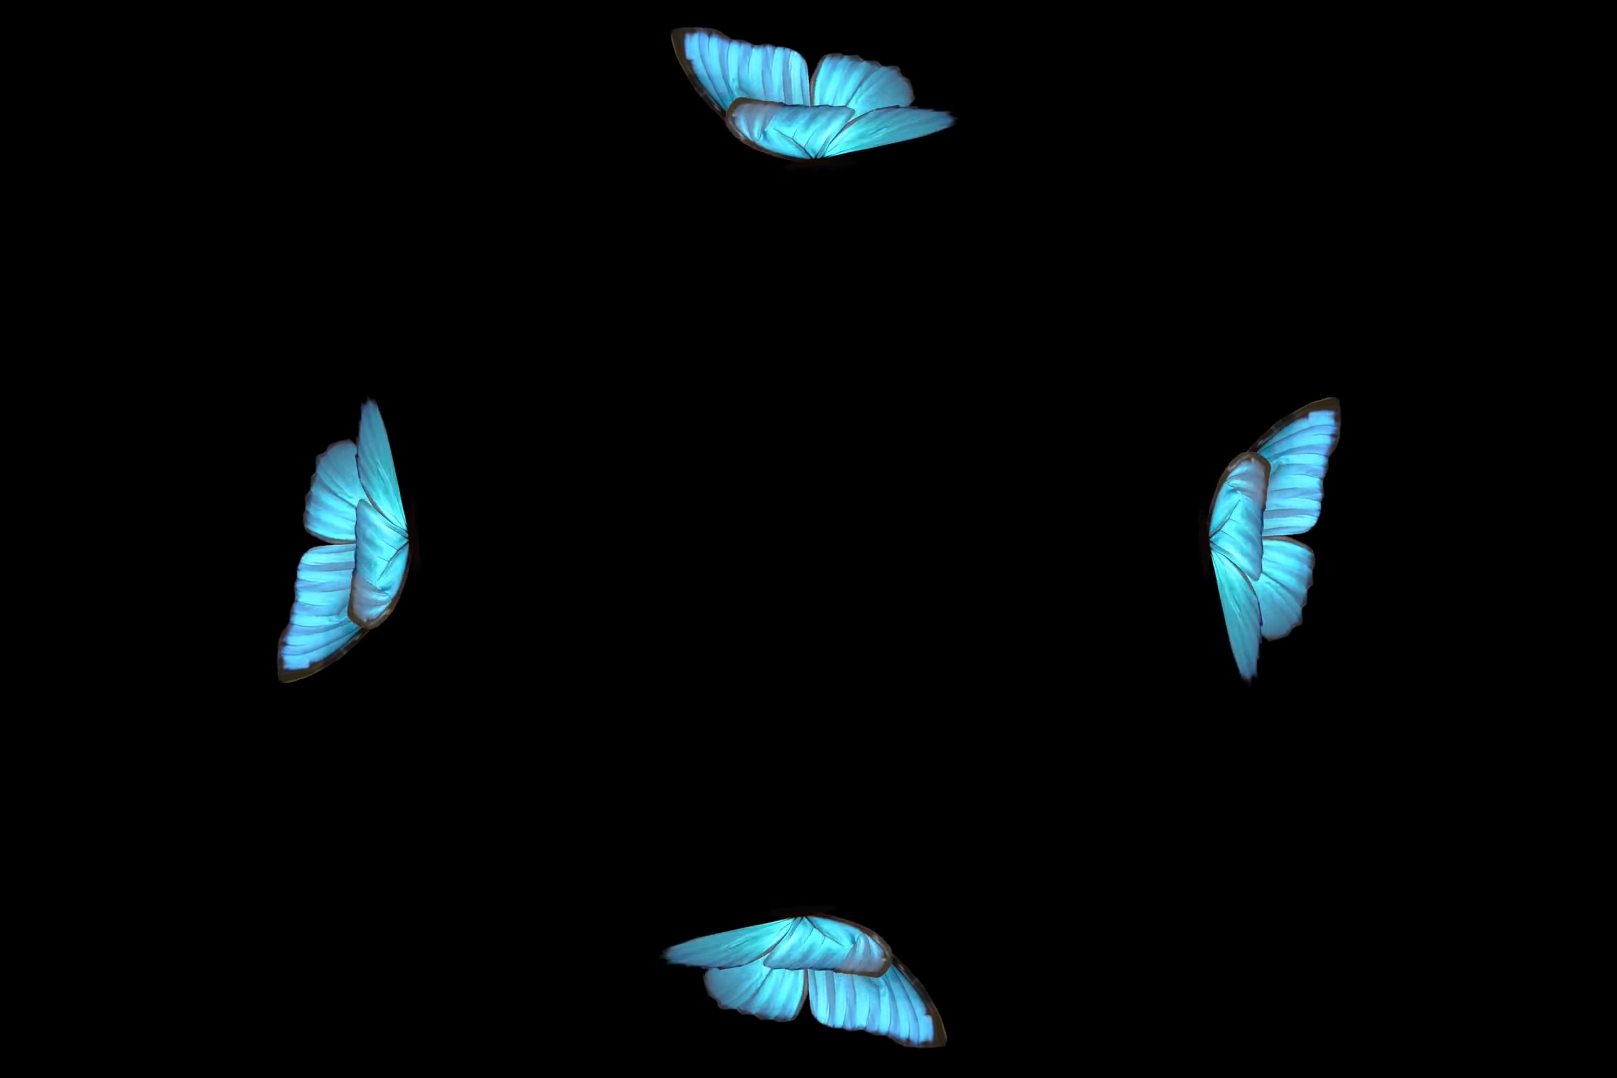
\includegraphics[width=0.47\textwidth]{img/bab2/p4_video.png}}
		\caption{Piramida 4 sisi}
		\label{fig:piramid4}
	\end{figure}
	
\vspace{2ex}

\section{\textit{Leap Motion Controller}}
\vspace{1ex}
	Leap Motion adalah sebuah perangkat yang dapat menggantikan \textit{mouse} maupun \textit{keyboard} tanpa harus menyentuhnya secara langsung. Leap Motion dihubungkan dengan komputer menggunakan USB 2.0  agar dapat membaca pergerakan tangan maupun jari yang diberikan oleh \textit{user}. Leap Motion berbeda dengan Kinect, dimana hanya informasi yang terbatas mengenai posisi tangan bukan \textit{depth map} seperti Kinect\cite{naidu2016hand}. Secara fisik, Leap Motion memiliki dimensi yang kecil yaitu 80 x 30 x 11,25 mm (3.1 x 1.2 x 0.5 inch) dengan bobot 3.2 gram. Dengan menggunakan 2 kamera monokrom yang berjarak 4cm dan 3 LED infrared, Leap Motion dapat melacak panjang gelombang 850 nanometer yang berada di luar spectrum cahaya tampak. Leap Motion memiliki jangkauan area sebesar 60 cm (2 ft) di atas \textit{controller}, 60 cm (2 ft) dengan sudut 150° untuk lebar setiap sisinya, dan 60 cm (2 ft) dengan sudut 120° untuk kedalaman setiap sisinya. Sedangkan \textit{interaction box} dalam sistem koordinatnya dapat menjangkau seluas 0.266 m³ (8 ft³) dengan bentuk piramida terbalik\cite{leapmotion_ds}. Keduanya dapat dilihat pada gambar \ref{fig:lm_int}.
	\begin{figure} [H]
		\subfloat[\textit{Interaction Area}\cite{leapmotionblog}.]{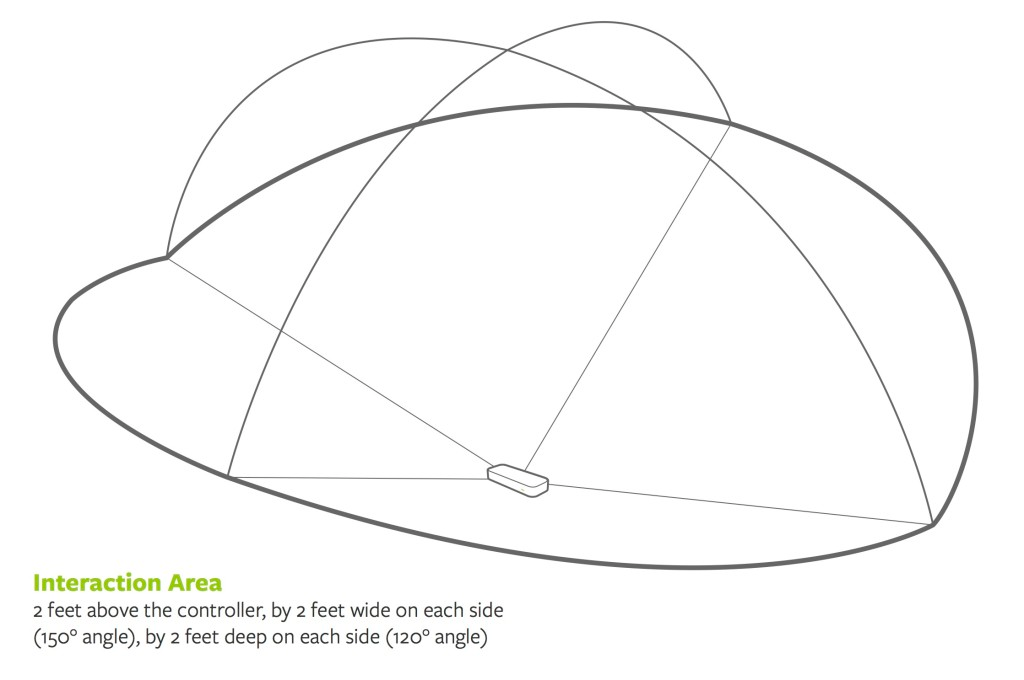
\includegraphics[width=0.47\textwidth]{img/bab2/lm_intarea.png}}
		\hspace{0.1em}
		\subfloat[\textit{Interaction Box}\cite{leapmotiondev}.]{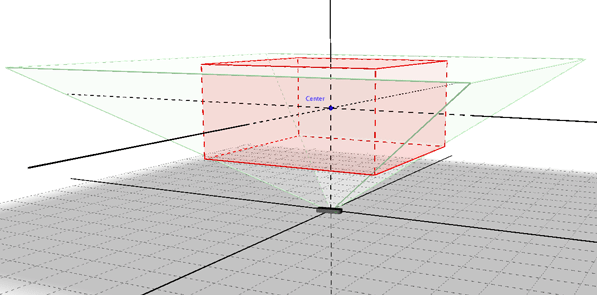
\includegraphics[width=0.47\textwidth]{img/bab2/lm_intbox.png}}
		\caption{Area yang dijangkau Leap Motion.}
		\label{fig:lm_int}
	\end{figure}
	Leap Motion dapat mengenali 27 bagian dari \textit{hand object elements} yang ditunjukkan pada gambar \ref{fig:handobject}. Elemen ini yang membuat Leap Motion dapat mengenali posisi tangan hingga dapat membaca \textit{motion} dan \textit{gesture}. \textit{Motion} atau pergerakan tangan didefinisikan sebagai \textit{continuous hand movements} yaitu memperkirakan posisi terhadap perubahan waktu, di antaranya \textit{scale}, \textit{rotation}, dan \textit{translation}. \textit{Gesture} didefinisikan sebagai perubahan pola yang dapat mentrigger aksi tertentu, di antaranya \textit{swipe}, \textit{circle}, dan \textit{tap}. Leap Motion bekerja dengan cara menangkap \textit{grayscale stereo image} yang dipisahkan berdasarkan kameran kanan dan kiri. Data tersebut disimpan dalam memori internalnya dan menjalankan penyesuaian resolusi. Kemudian dikirimkan via USB menuju Leap Motion Software untuk diolah datanya.
	\begin{figure} [H]
		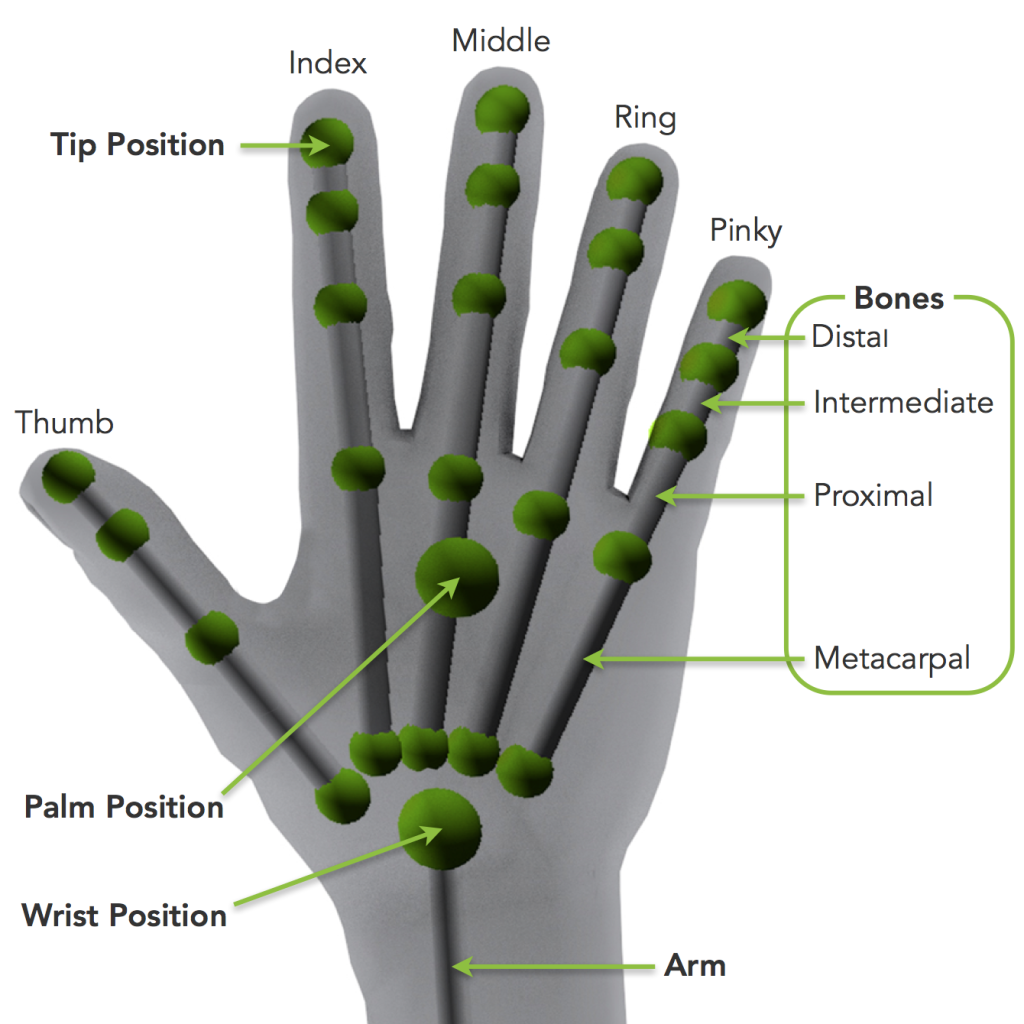
\includegraphics[scale=0.25]{img/bab2/handobject.png}
		\caption{\textit{Hand object elements} pada Leap Motion.}
		\label{fig:handobject}
	\end{figure}
\vspace{2ex}

\cleardoublepage
\chapter{DESAIN DAN IMPLEMENTASI SISTEM}
\vspace{4ex}

\hspace{\parindent} Penelitian ini dilaksanakan sesuai dengan desain sistem serta implementasinya. Desain sistem merupakan konsep dari pembuatan dan perancangan infrastruktur kemudian diwujudkan dalam bentuk blok-blok alur yang harus dikerjakan. Implementasi merupakan pelaksanaan teknis untuk setiap blok pada desain sistem.
\vspace{2ex}

\section{Gambaran Umum}
\vspace{1ex}
	Penelitian ini bertujuan untuk merancang dan menerapkan interaksi berdasarkan \textit{hand gesture} pada hologram 3D. Sistem ini dikemas dalam satu set yang terdiri dari \textit{pyramid hologram}, Leap Motion, \textit{display monitor}, \textit{information monitor} beserta \textit{server computer} seperti pada gambar \ref{fig:cara_kerja}.
	\begin{figure} [H]
		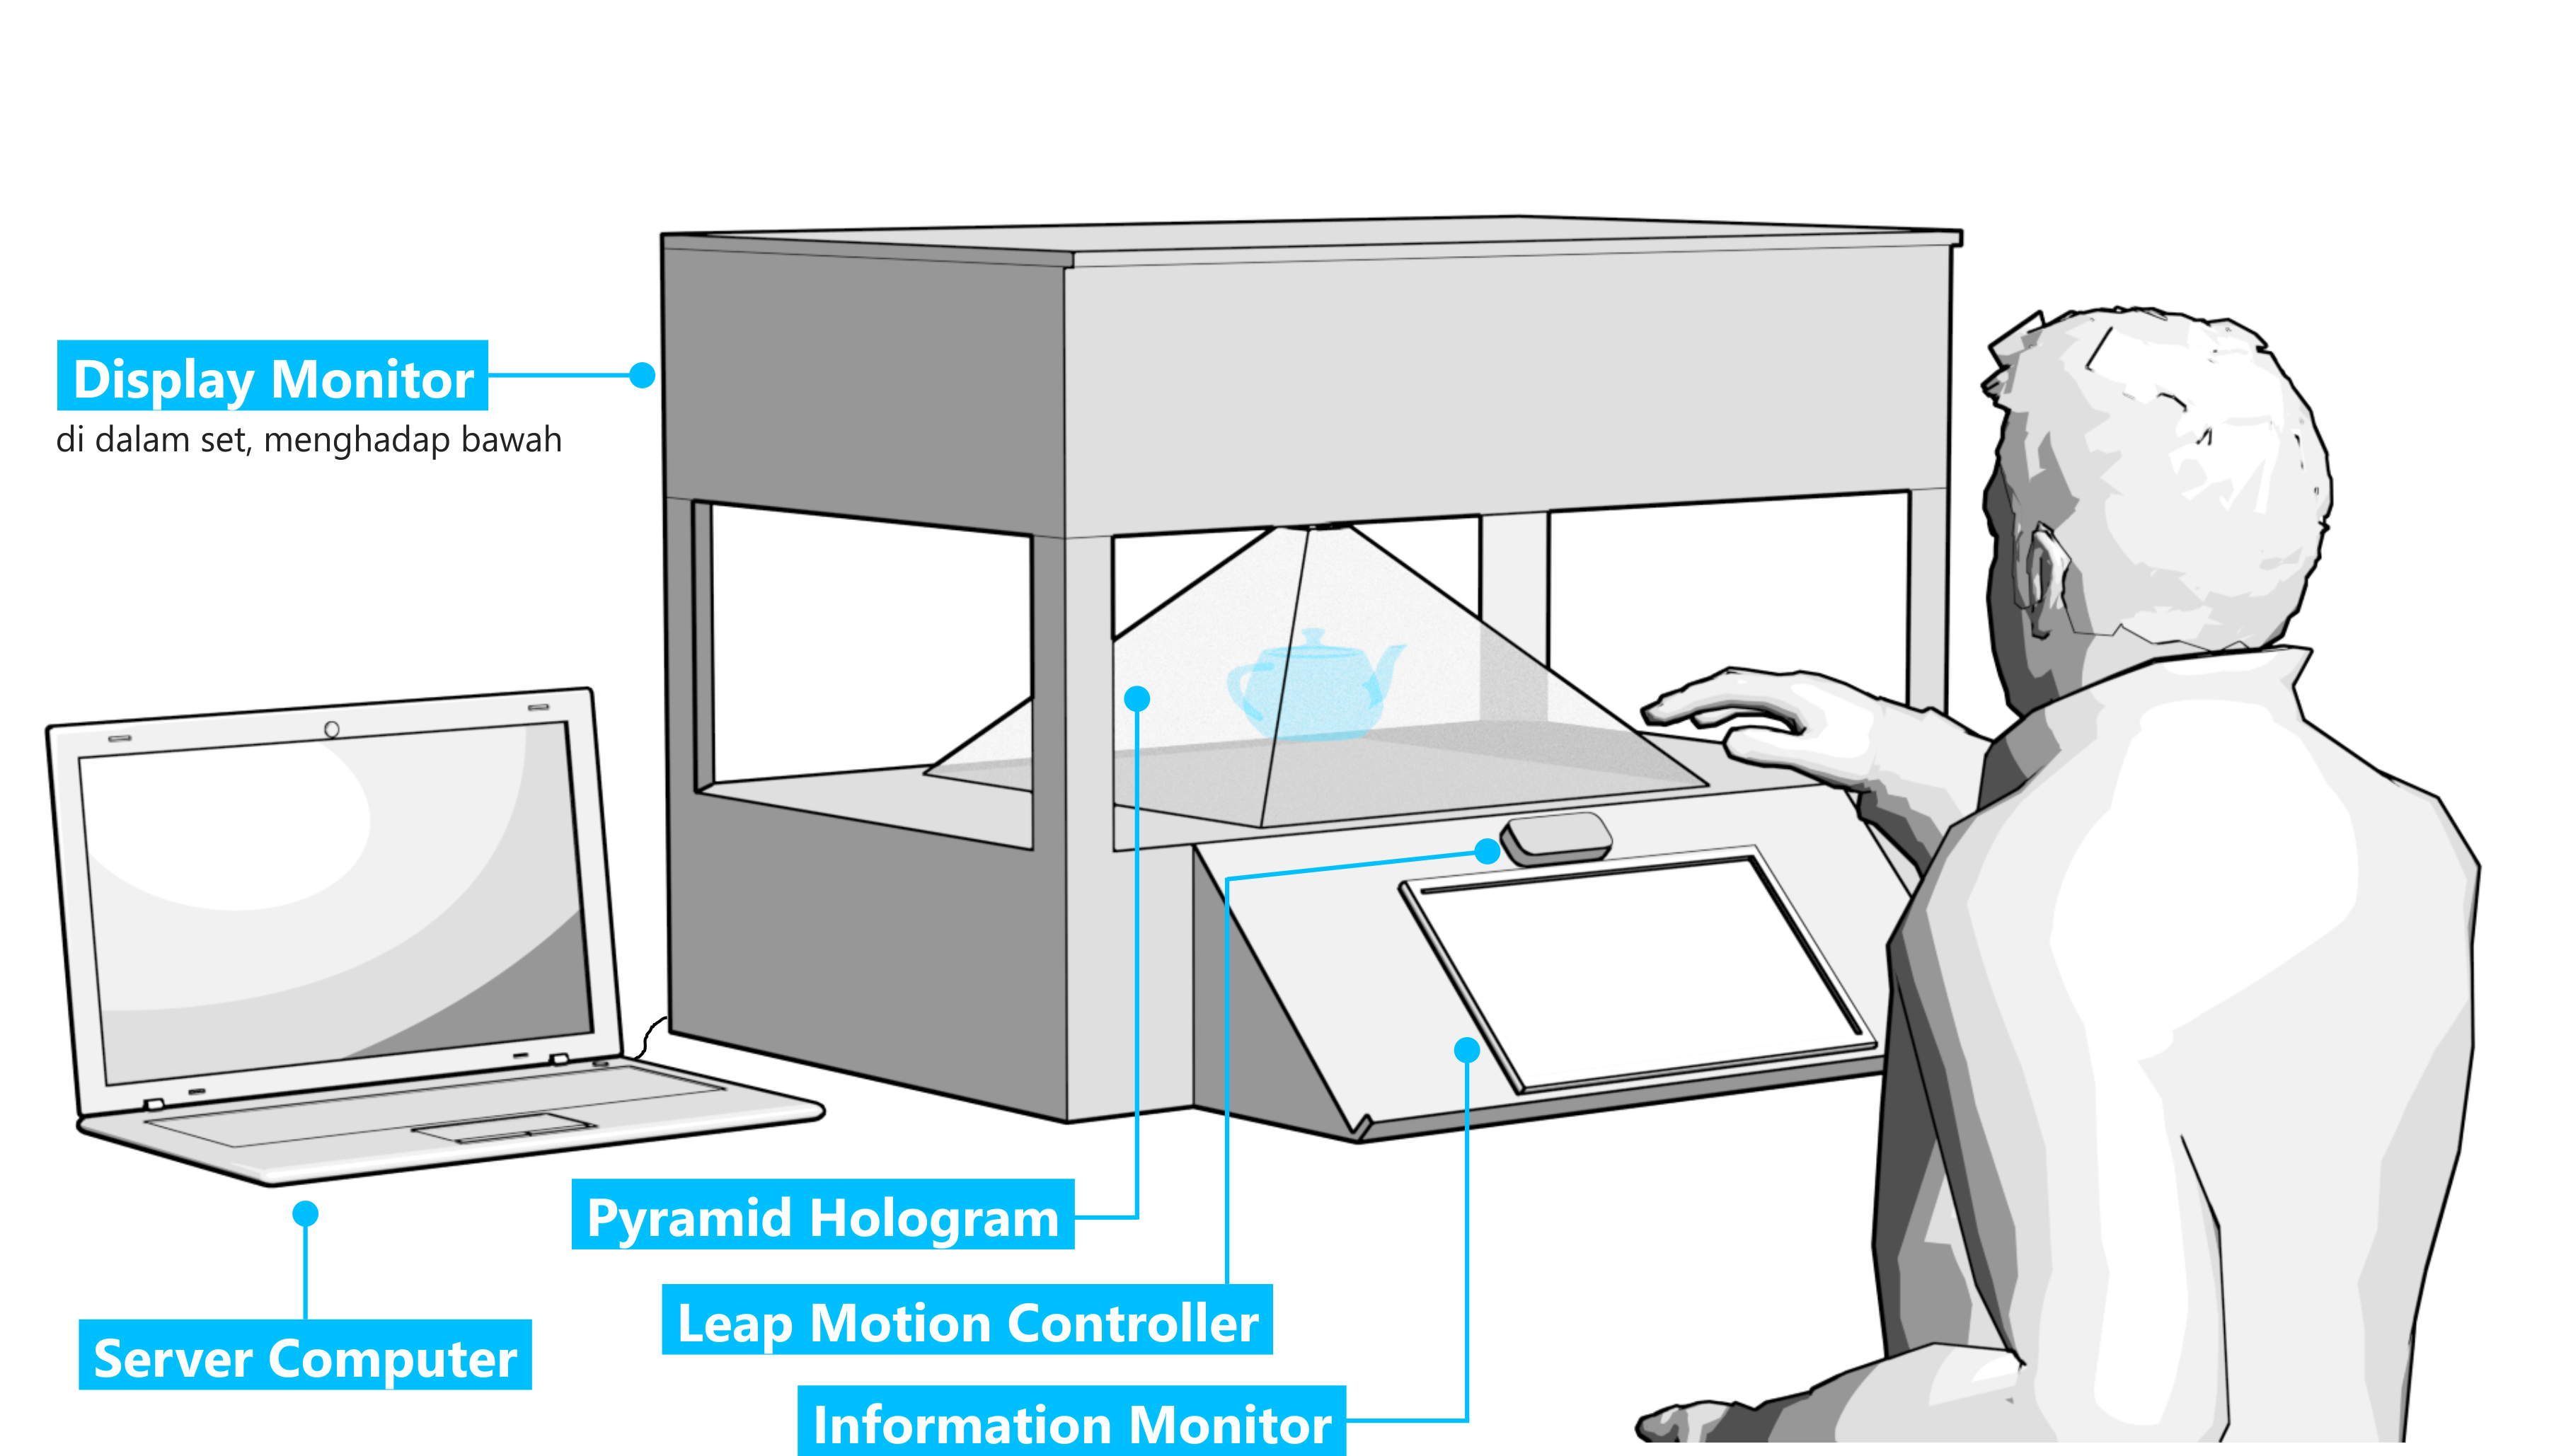
\includegraphics[width=\textwidth]{img/bab3/cara_kerja.png}
		\caption{Gambaran umum penggunaan sistem.}
		\label{fig:cara_kerja}
	\end{figure}
	\textit{Display monitor} dan \textit{pyramid hologram} di bawahnya menampilkan objek hologram 3D sedangkan \textit{information monitor} menampilkan informasi mengenai program yang dijalankan. Leap Motion yang terletak di atas \textit{information monitor} menangkap pergerakan tangan pengguna. \textit{Server computer}  mengolah data dan menentukan fitur yang diaktifkan. Berdasarkan data yang diperoleh maka objek hologram dapat menampilkan respons dan memungkinkan pengguna melakukan interaksi.
\vspace{2ex}

\section{Desain Sistem}
\vspace{1ex}
	Pada sistem ini pengguna dapat melakukan interaksi dengan hologram menggunakan Leap Motion. Objek hologram yang diperlihatkan melalui pantulan dari monitor terhadap \textit{pyramid hologram} dapat merespons sesuai \textit{hand gesture} dari pengguna. Kemudian informasi mengenai objek hologram tersebut juga ditampilkan. Alur kerja dari sistem ini dijelaskan melalui gambar \ref{fig:alur_kerja}.
	\vspace{-2ex}
	\begin{figure} [H]
		
\includegraphics[scale=0.25]{img/bab3/alur_kerja.png}
		\caption{Alur kerja penggunaan sistem.}
		\label{fig:alur_kerja}
	\end{figure}
	\vspace{-2ex}
	Terdapat dua sub-sistem yang membangun tujuan dari penelitian ini, yaitu sistem virtualisasi mengenai pembangunan aplikasi termasuk rekonstruksi objek 3D menjadi bentuk hologram maupun \textit{user interface} untuk informasinya dan sistem interaksi tentang bagaimana pengguna dapat memberikan input terhadap objek hologram. Agar kedua sub-sistem ini dapat berfungsi bersamaan, maka dibutuhkan perancangan desain \textit{storyboard} penggunaan serta setting perangkat.
\vspace{1.5ex}

	\subsection{Desain \textit{Storyboard}}
	\vspace{1ex}
		\textit{Storyboard} yang diterapkan pada penelitian ini dirancang berdasarkan alur yang akan dilakukan oleh pengguna saat menggunakan perangkat. Alur penggunaan perangkat ini dijelaskan melalui tahapan sebagai berikut :
		\begin{enumerate}[nolistsep]
			\item Ketika pengguna menggunakan perangkat, kedua monitor menampilkan bagian awal aplikasi. \textit{Display monitor} menampilkan sebuah objek hologram yang berputar. Sedangkan \textit{information monitor} menampilkan \textit{Main Menu} aplikasi.
			\item Ketika memilih tombol "Start", kedua monitor memberikan panduan mengenai cara penggunaan dan gestur dasar yang dibangun pada sistem ini.
			\item Setelah menyelesaikan tutorial panduan, kedua monitor menampilkan koleksi objeknya satu persatu.  Objek-objek yang ditampilkan secara berurutan adalah \textit{Hand Axe}, \textit{Primeval Axe}, \textit{Buddha Statue}, \textit{Ganesha Statue}, \textit{Brass Lamp}, \textit{Ceramic Pot}, \textit{Typewriter}, dan \textit{Gramaphone}.
			\item Pengguna dapat melakukan interaksi terhadap objek hologram yang ditampilkan melalui \textit{display monitor} dan mendapatkan informasi mengenai profil objek tersebut melalui \textit{information monitor}.
			\item Interaksi yang antara pengguna dan onjek hologram terjadi selama dilakukan dalam jangkauan Leap Motion. Objek hologram akan memberikan respons sesuai interaksi yang diberikan.     
			\item Pengguna dapat melihat informasi mengenai objek aslinya melalui \textit{information monitor}. Selain itu, pengguna dapat memilih objek sebelum ataupun setelahnya untuk ditampilkan melalui tombol yang tersedia.
			\item Pada \textit{information monitor} juga memberikan informasi bahwa objek hologram tersebut dilengkapi dengan animasi yang diaktifkan melalui gestur tertentu. Ketika gestur diberikan, maka objek hologram akan menampilkan responsnya.
			\item Eksplorasi akan berakhir ketika pengguna memilih tombol "Main Menu" dan kembali ke menu awal aplikasi.
		\end{enumerate}	
	\vspace{1.5ex}
	
	\subsection{Desain Setting Perangkat}
	\vspace{1ex}
		Dalam membangun sistem ini, diperlukan suatu set yang dapat berfungsi untuk melakukan visualisasi objek hologram 3D dan sensor pengindera tangan. Masing-masing perangkat yang dimuat dalam set memiliki spesifikasi sebagai berikut :
		\begin{enumerate}[nolistsep]
			\item \textit{Display Monitor}
			
			Berfungsi untuk menampilkan objek 3D yang telah direkonstruksi dalam bentuk \textit{hologram video}.
			\vspace{-2ex}
			\begin{table}[H]
				\begin{flushleft}
				\begin{tabular}{L{0.5cm} l L{2.55cm} l}
					&\textbullet & Nama 			& : COOCAA 32 inch TV LED \\
					&\textbullet & Resolusi 		& : 1366 x 768 (\textit{HD Ready}) \\
					&\textbullet & \textit{Connection Slot}	& : 2 HDMI \& 1 USB \\
					&\textbullet & Ukuran Layar & : 70 x 39 cm (32 inch) \\
					&\textbullet & Ukuran Total & : 74 x 45 x 10 cm \\
					&\textbullet & Berat 		& : 11 kg \\
				\end{tabular}
				\end{flushleft}
			\end{table}
			\vspace{-3.5ex}
			
			\item \textit{Information Monitor}
			
			Berfungsi untuk menampilkan informasi objek hologram yang ditayangkan.
			\vspace{-2ex}
			\begin{table}[H]
				\begin{flushleft}
					\begin{tabular}{L{0.5cm} l L{2.55cm} l}
						&\textbullet & Nama 		& : Desklab Ultralight Portable\\
						&  &  &  \         \     4K Touchscreen Monitor LED \\
						&\textbullet & Resolusi 	& : 3840 x 2160 (4K UHD)\\
						&\textbullet & \textit{Connection Slot}	& : 1 HDMI, 2 USB-C, \& 1 Micro USD \\
						&\textbullet & Ukuran Layar & : 70 x 39 cm (15.6 inch) \\
						&\textbullet & Ukuran Total & : 35 x 20 x 0.6 cm\\
						&\textbullet & Berat 		& : 0.6 kg \\
					\end{tabular}
				\end{flushleft}
			\end{table}
			\vspace{-3.5ex}
			
			\item \textit{Server Computer}
			
			Berfungsi untuk melakukan komputasi baik visual yang ditampilkan pada kedua monitor maupun mengolah data interaksi dari Leap Motion.
			\vspace{-2ex}
			\begin{table}[H]
				\begin{flushleft}
				\begin{tabular}{L{0.5cm} l L{2.55cm} l}
						&\textbullet & Nama 			& : Asus ROG Strix GL553VD \\
						&\textbullet & \textit{Processor}		& : Intel Core i7 7700HQ \\
						&\textbullet & \textit{Graphic Card}	& : NVIDIA GeForce GTX 1050 \\
						&\textbullet & \textit{Connection Slot}	& : 1 HDMI, 2 USB 3.0, 1 USB 3.1\\
						&  &  & \         \     1 USB 2.0 \\
						&\textbullet & RAM				& : 16 GB \\
						&\textbullet & Resolusi			& : 1920 x 1080 (15.6 inch)\\
					\end{tabular}
				\end{flushleft}
			\end{table}
			\vspace{-3.5ex}
		
			\item \textit{Pyramid Hologram}
			
			Berfungsi untuk merefleksikan objek dari \textit{display monitor} sehingga membentuk 3D hologram.
			\begin{comment}
			\vspace{-2ex}
			\begin{table}[H]
				\begin{flushleft}
				\begin{tabular}{L{0.5cm} l L{2.55cm} l}
					&\textbullet & Material & : Akrilik Ryben 2 mm \\
					&\textbullet & Ukuran 	& : 39 x 39 x 19.5 cm
				\end{tabular}
				\end{flushleft}
			\end{table}
			\vspace{-3.5ex}
			\end{comment}
			
			\item \textit{Leap Motion Controller}
			
			Berfungsi sebagai sensor pengindera tangan untuk input dari pengguna\cite{leapmotion_ds}.
			\vspace{-2ex}
			\begin{table}[H]
				\begin{flushleft}
				\begin{tabular}{L{0.5cm} l L{2.55cm} l}
					&\textbullet & Ukuran  						& : 8 x 3 x 1.2 cm (3.1 x 1.2 x 0.5 inch) \\	
					&\textbullet & Berat						& : 32 gr (1.6 oz) \\
					&\textbullet & \textit{Connection} 			& : \textit{wired} (USB 2.0)\\
					&\textbullet & \textit{Interaction Area} 	& : 60cm \textit{from above controller}\\
					&  &  &  \         \      60 cm \& 150° \textit{from each side's width}  \\	
					&  &  &  \         \     60 cm \& 120° \textit{from each side's depth}   \\	
				\end{tabular}
				\end{flushleft}
			\end{table}
			\vspace{-3.5ex}
		\end{enumerate}
		\vspace{-2ex}
		\begin{figure} [H]
			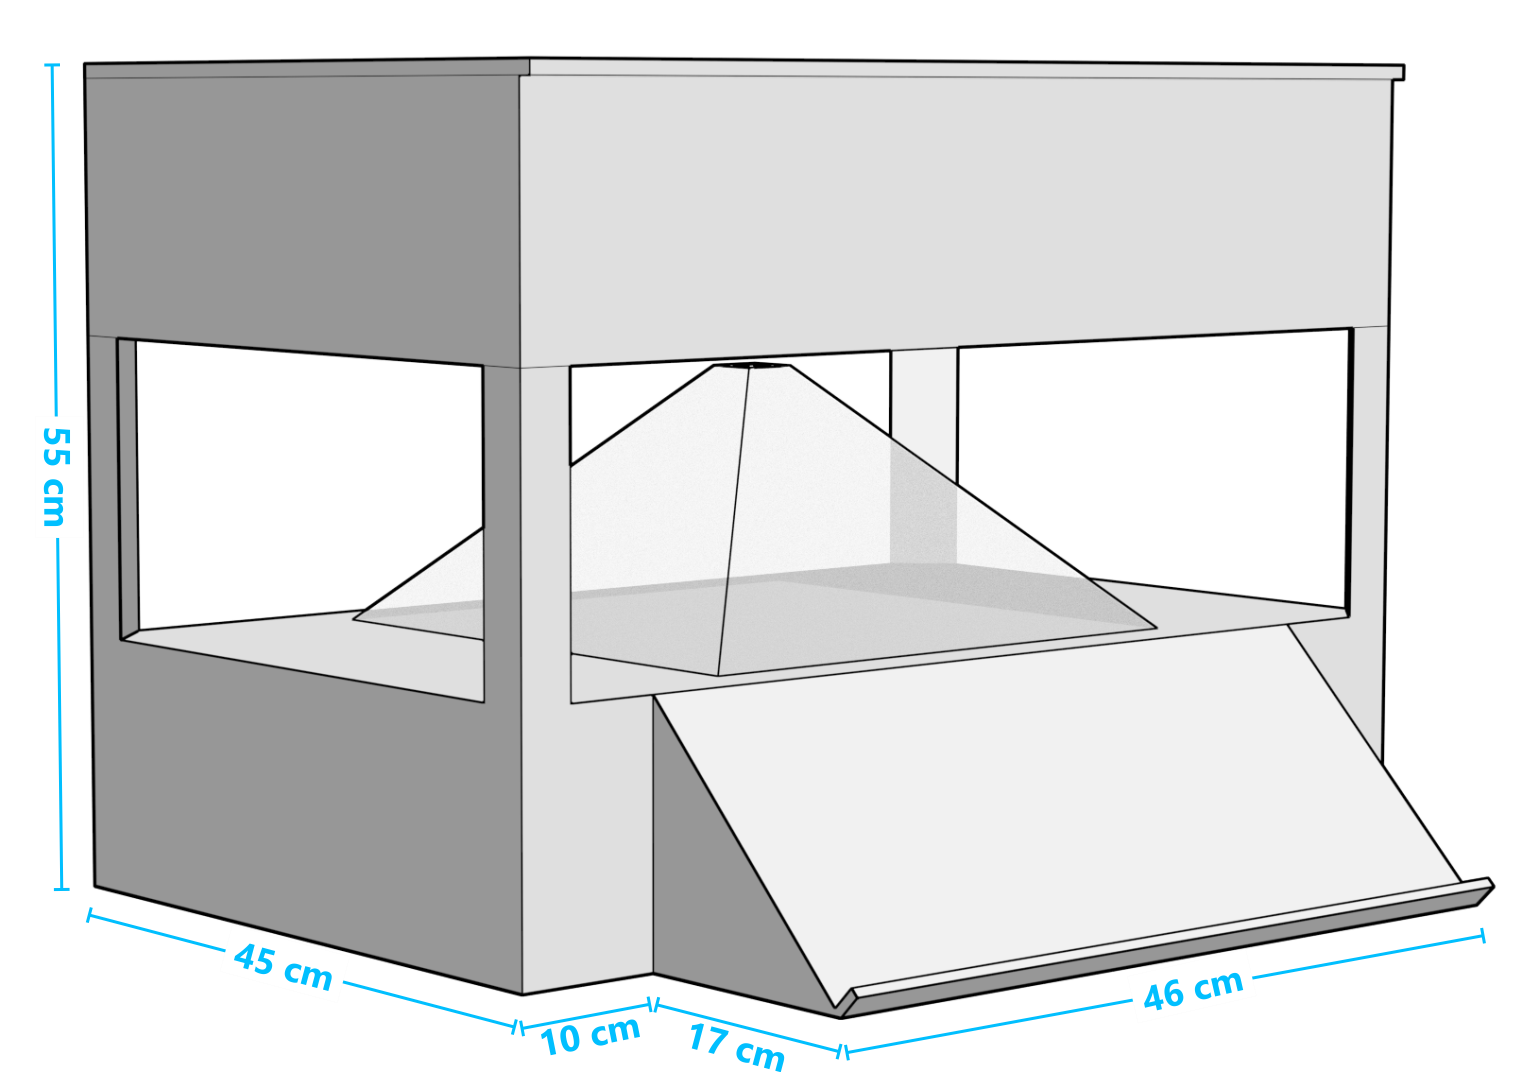
\includegraphics[width=0.75\textwidth]{img/bab3/desain_perangkat.png}
			\caption{Desain setting perangkat.}
			\label{fig:desain_setting}
		\end{figure}
		\vspace{-2ex}
		Penjelasan detail dari set yang dirancang dijelaskan melalui gambar \ref{fig:desain_setting}. Setting perangkat ini terdiri dari 3 bagian utama. Pada bagian atas, semua sisi tertutup kecuali sisi penompang \textit{display monitor} yang dilapisi dengan spons busa untuk menghindari kerusakan pada layar monitor. Di sisi berlawanannya dapat dibuka dan ditutup untuk memindahkan \textit{display monitor} dari set. Pada bagian tengah dibangun oleh penyangga di setiap sudut, dimana salah satunya menjadi jalur pengkabelan. \textit{Pyramid hologram} diposisikan di sisi tengah pada bagian ini dengan sisi terkecilnya menghadap \textit{display monitor}. \textit{Pyramid hologram} ini akan memantulkan \textit{hologram video} tepat pada bagian dalam. Leap Motion diletakkan pada sisi depan set yang terdapat sisi miring yang juga menompang \textit{information monitor}. Semua pengkabelan dari \textit{display monitor}, Leap Motion, serta \textit{information monitor} berpusat di bagian bawah set yang kemudian keluar melalui sisi belakang untuk disambungkan dengan \textit{server computer} beserta sumber listrik. Untuk menghindari adanya pantulan cahaya yang dapat mengganggu objek hologram yang dibentuk, setting perangkat dilapisi dengan stiker hitam polos di setiap sisi bagiannya.
	\vspace{1ex}
	
		\subsubsection{Desain \textit{Pyramid Hologram}}
		\vspace{0.5ex}
			Perancangan \textit{pyramid hologram} diperlukan agar hologram yang direfleksikan dapat tervisualisasikan dengan ukuran yang sesuai harapan. Prinsip kerja dari \textit{pyramid hologram} ini ditampilkan melalui gambar \ref{fig:prinsip_piramid}. Pada penelitian ini, jenis \textit{pyramid hologram} yang digunakan yaitu dengan piramid 4 sisi yang menghasilkan 4 objek jatuh di tengah-tengah piramid. Berdasarkan hal tersebut maka membutuhkan 4 buah segitiga sama kaki yang membentuk piramid dengan alas berbentuk persegi yang ukuran maksimalnya sebesar lebar monitor ($\ell$) yang digunakan dengan tinggi piramida sebesar setengah lebar monitor($\frac{1}{2}\ell$) membentuk sudut 45° antara sisi segitiga dengan \textit{display monitor}. Pemotongan pucuk piramida yang digunakan pada penelitian ini adalah sebesar sepersepuluh dari alas piramida.
			\begin{figure} [H]
				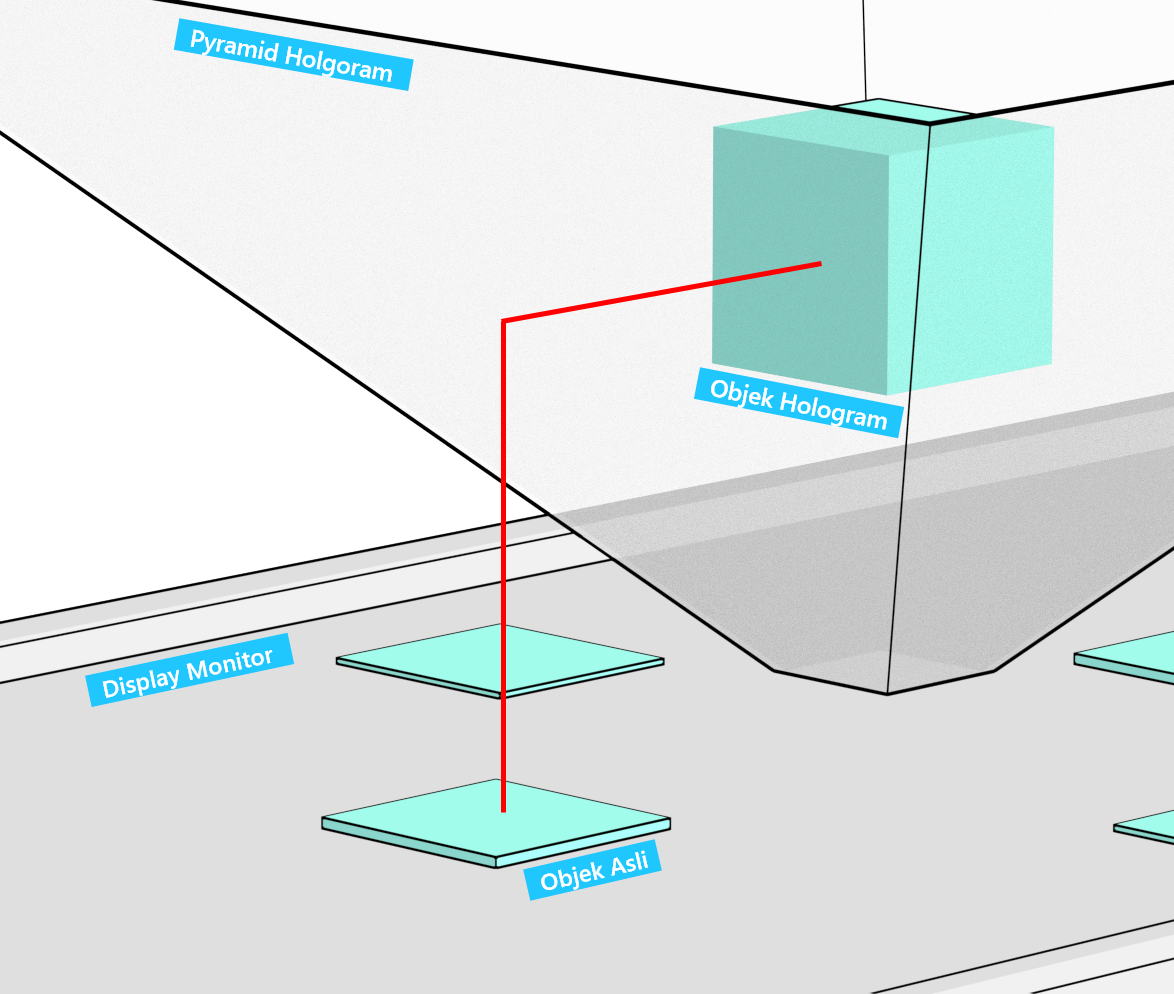
\includegraphics[width=0.6\textwidth]{img/bab3/prinsip_piramid.png}
				\caption{Prinsip \textit{pyramid hologram}.}
				\label{fig:prinsip_piramid}
			\end{figure}
			\vspace{-2ex}
			
			\begin{figure} [H]
				\subfloat[Perbandingan piramida dan objek hologram. \label{fig:piramida4}]{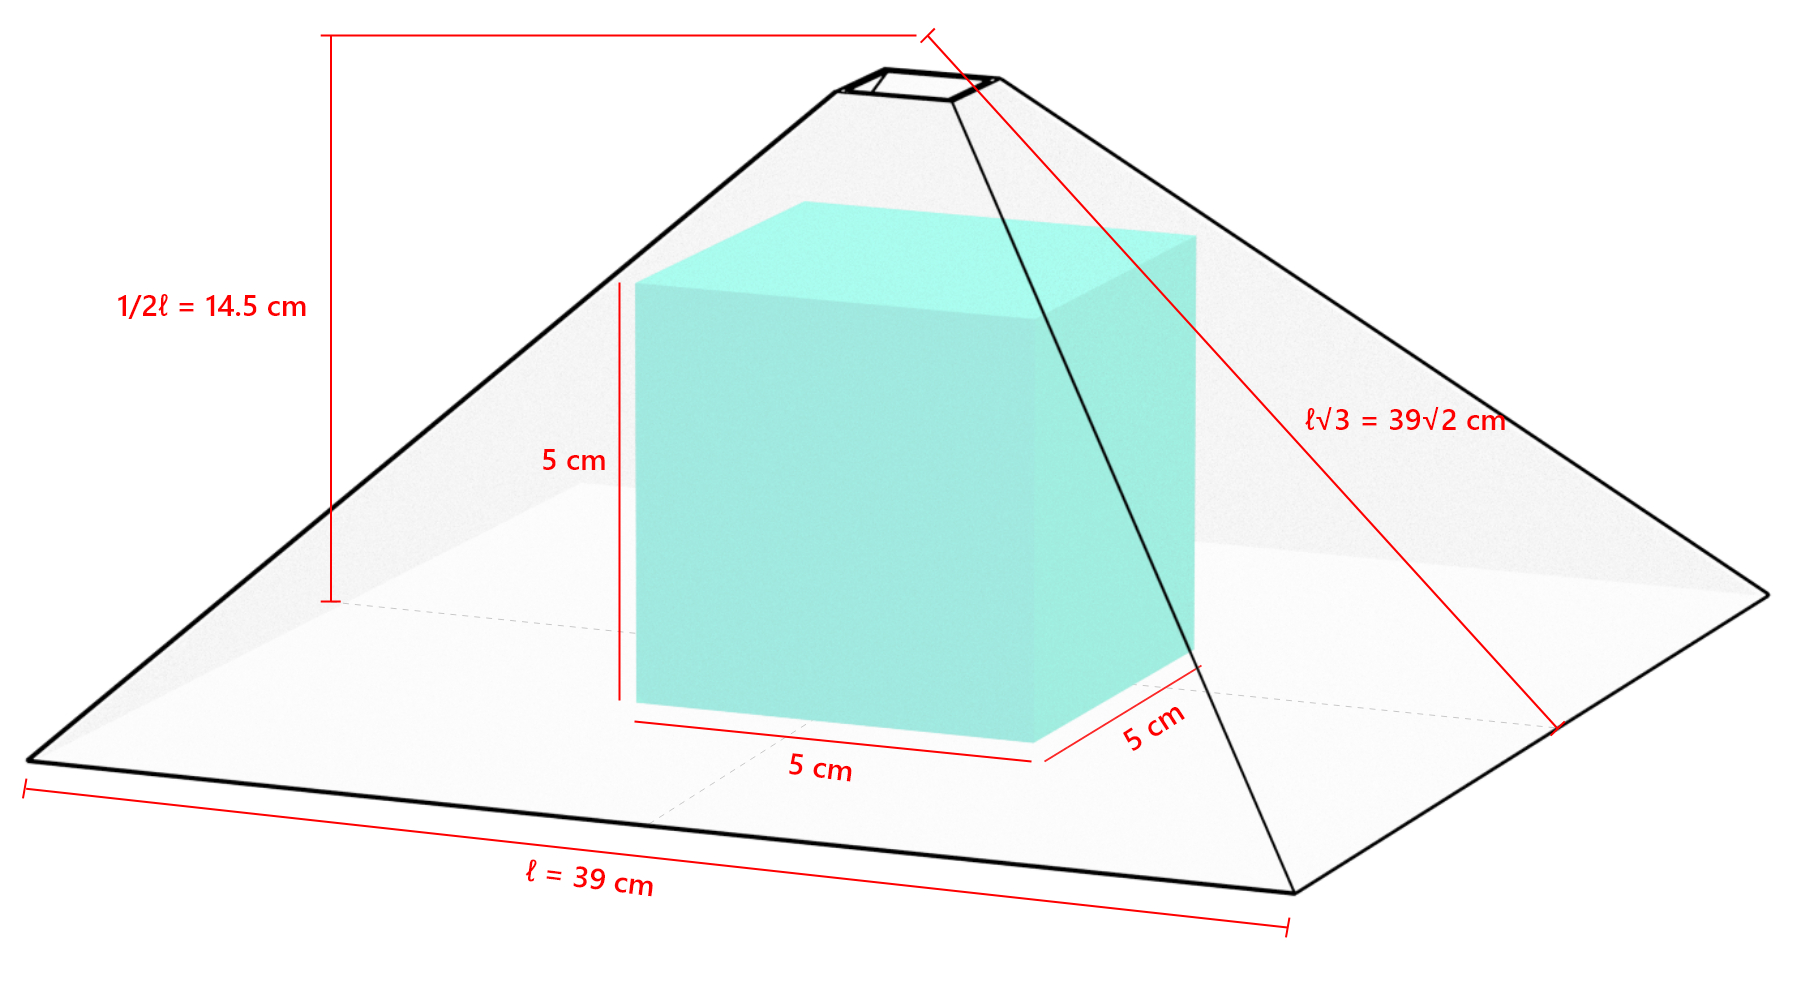
\includegraphics[width=0.85\textwidth]{img/bab3/piramida4.png}}
				\hspace{0.1em}
				\subfloat[Segitiga piramida awal. \label{fig:piramida2}]{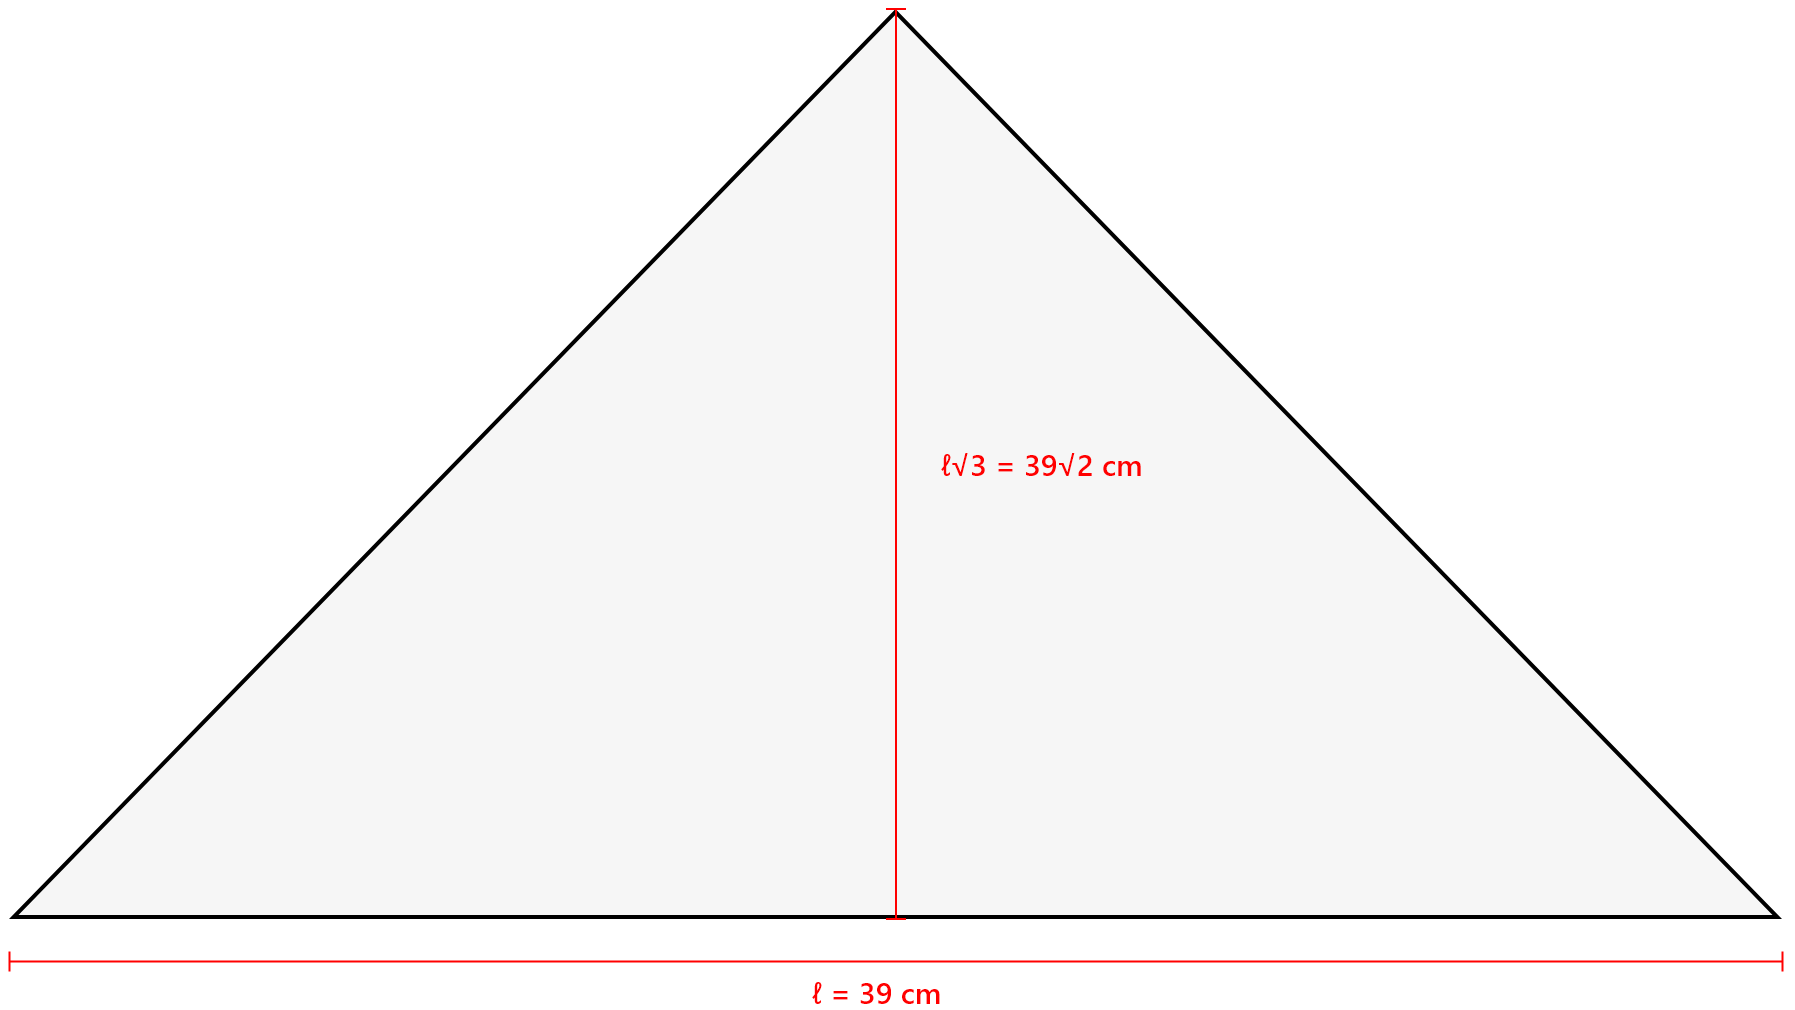
\includegraphics[width=0.55\textwidth]{img/bab3/piramida2.png}}
				\hspace{0.1em}
				\subfloat[Segitiga piramida akhir. \label{fig:piramida3}]{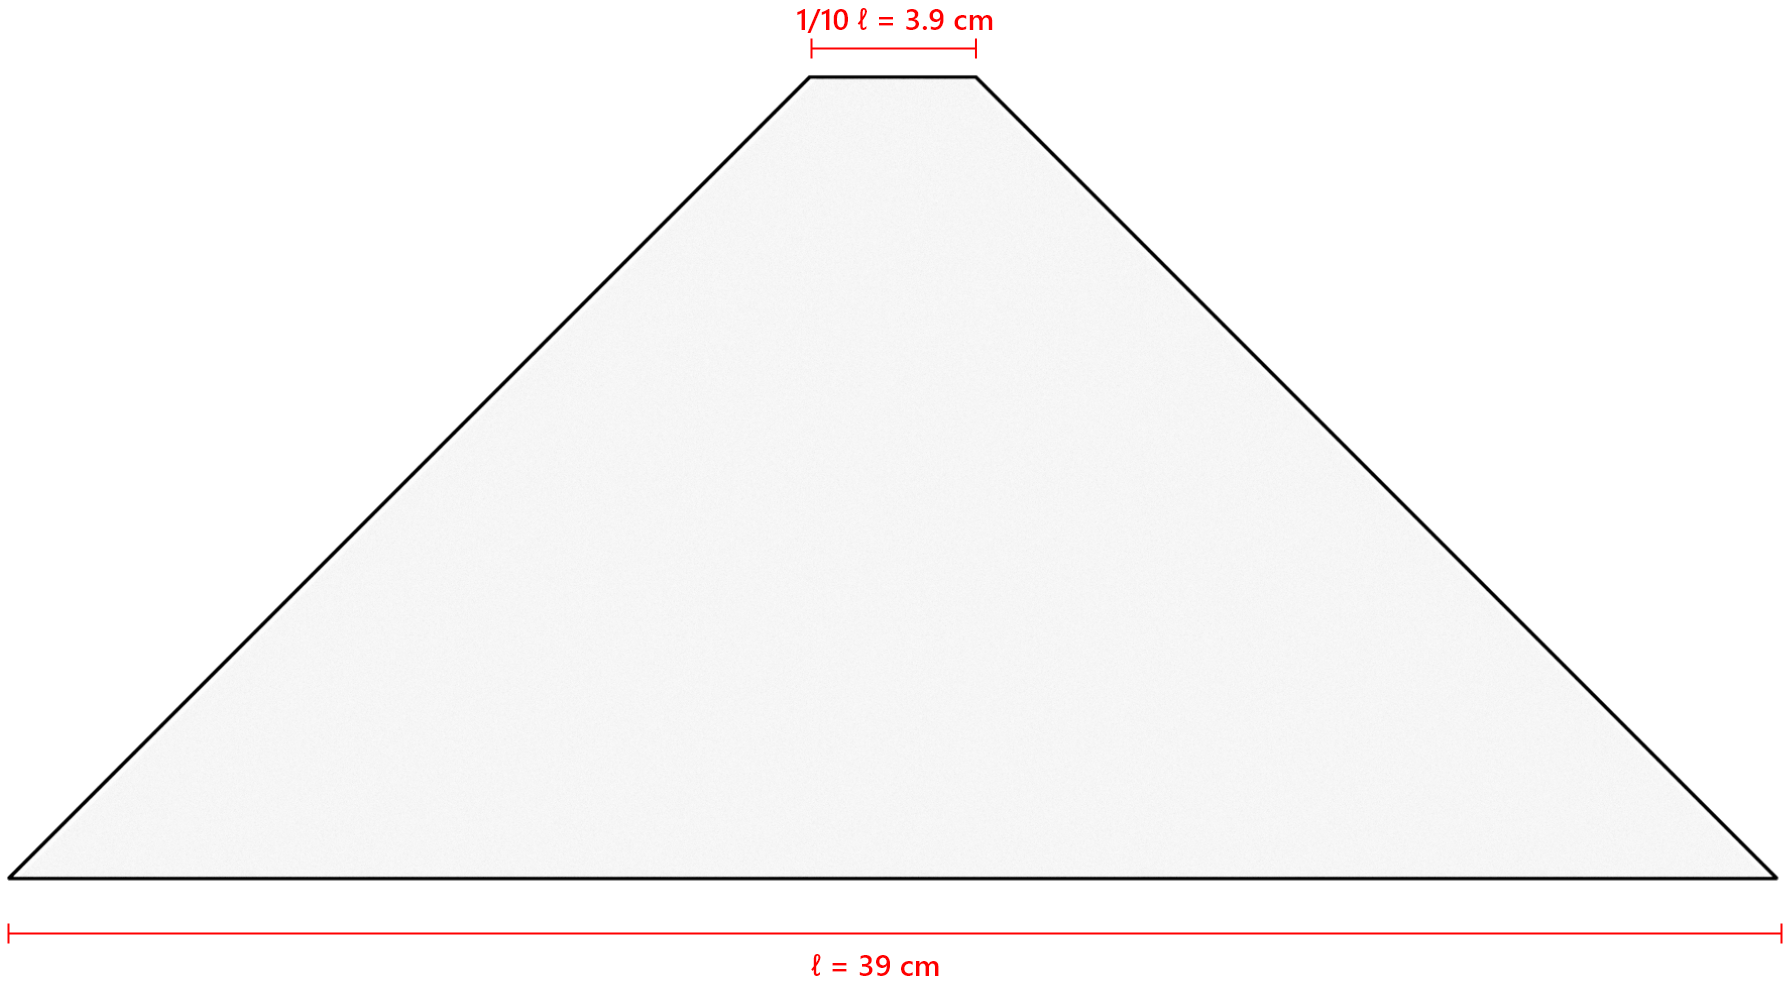
\includegraphics[width=0.55\textwidth]{img/bab3/piramida3.png}}
				\caption{Desain gestur yang membangun sistem interaksi.}
				\label{fig:desainpiramida}
			\end{figure}
			\vspace{-2ex}
		
			Sehingga desain \textit{pyramid hologram} yang diterapkan pada penelitian ini ditunjukkan melalui gambar \ref{fig:desainpiramida}. Dengan alas piramida berbentuk pesergi sebesar lebar monitor = 39 cm, maka tinggi piramida = 14.5 cm sesuai gambar \ref{fig:piramida4}. Kemudian untuk setiap sisi segitiganya memiliki alas = 39 cm dengan tinggi $39\sqrt{2}$ sesuai gambar \ref{fig:piramida2}. Terakhir, segitiga dipotong dengan sisi terpendeknya membentuk ukuran 3.9cm sesuai gambar \ref{fig:piramida3}. Dengan piramid seperti ini, maka besar objek hologram yang dapat diamati kurang dari 14.5 cm, idealnya adalah 5 x 5 x 5 cm sesuai gambar \ref{fig:piramida4} mendekati seperdelapan (7.8) dari lebar monitor yang digunakan. Bahan yang digunakan untuk membuat \textit{pyramid hologram} adalah akrilik ryben (hitam tembus pandang) yang berukuran 2 mm.
		%\vspace{0.75ex}
	\vspace{1.5ex}
	
	\subsection{Desain Sistem Visualisasi}
	\vspace{1ex}
		Sistem visualisasi yang diterapkan pada penelitian ini berkaitan dengan penyajian aplikasi di \textit{display} dan \textit{information monitor}. \textit{Display monitor} menampilkan \textit{hologram video}. \textit{Hologram video} akan terlihat sebagai bentuk objek hologram karena adanya refleksi cahaya dari setiap sisi \textit{pyramid hologram}. Sedangkan \textit{information monitor} menampilkan informasi dan \textit{interface} aplikasi. \textit{Information monitor} juga menerima inputan dari pengguna untuk mengatur aplikasi melalui tombol yang disediakan. Alur kerja dari sistem visualisasi yang diterapkan ditunjukkan pada gambar \ref{fig:desain_visualisasi}.
		\begin{figure} [H]
			
\includegraphics[width=\textwidth]{img/bab3/desain_visualisasi.png}
			\caption{Alur kerja sistem visualisasi.}
			\label{fig:desain_visualisasi}
		\end{figure}
		\vspace{-2ex}
		
		Tampilan utama kedua monitor saat permainan dimulai ditunjukkan pada gambar \ref{fig:desain_monitor}. Hologram video pada \textit{display monitor} menampilkan 4 sisi objek yang ketika diproyeksikan menghasilkan objek hologram sesuai dengan gambar \ref{fig:proyeksihologram}. Penempatan informasi objek pada \textit{information monitor} ditunjukkan pada gambar \ref{fig:desain_im}.
		
		Selain menampilkan informasi objek, \textit{information monitor} juga menampilkan \textit{user interface} aplikasi. Aplikasi terbagi menjadi dua bagian utama yang ditunjukkan pada gambar \ref{fig:storyboard}. \textit{Main Menu} atau Menu Utama merupakan tampilan awal saat aplikasi tersebut dijalankan. Bagian ini terdiri dari beberapa pilihan menu yang dapat diakses oleh pengguna, di antaranya \textit{How to Play} untuk menunjukkan cara penggunaan perangkat, \textit{About} untuk menunjukkan informasi mengenai produk dan developer, dan \textit{Exit} untuk keluar dari permainan. Sedangkan opsi \textit{Start} yang akan memulai bagian \textit{Main Scene} berupa \textit{scene} utama atau \textit{gameplay}.
		\vspace{-2ex}
		\begin{figure} [H]
			\subfloat[Tampilan \textit{Display Monitor}. \label{fig:desain_dm}]{
\includegraphics[width=0.6\textwidth]{img/bab3/desain_dm.png}}
			\hspace{0.1em}
			\subfloat[Tampilan \textit{Information Monitor}. \label{fig:desain_im}]{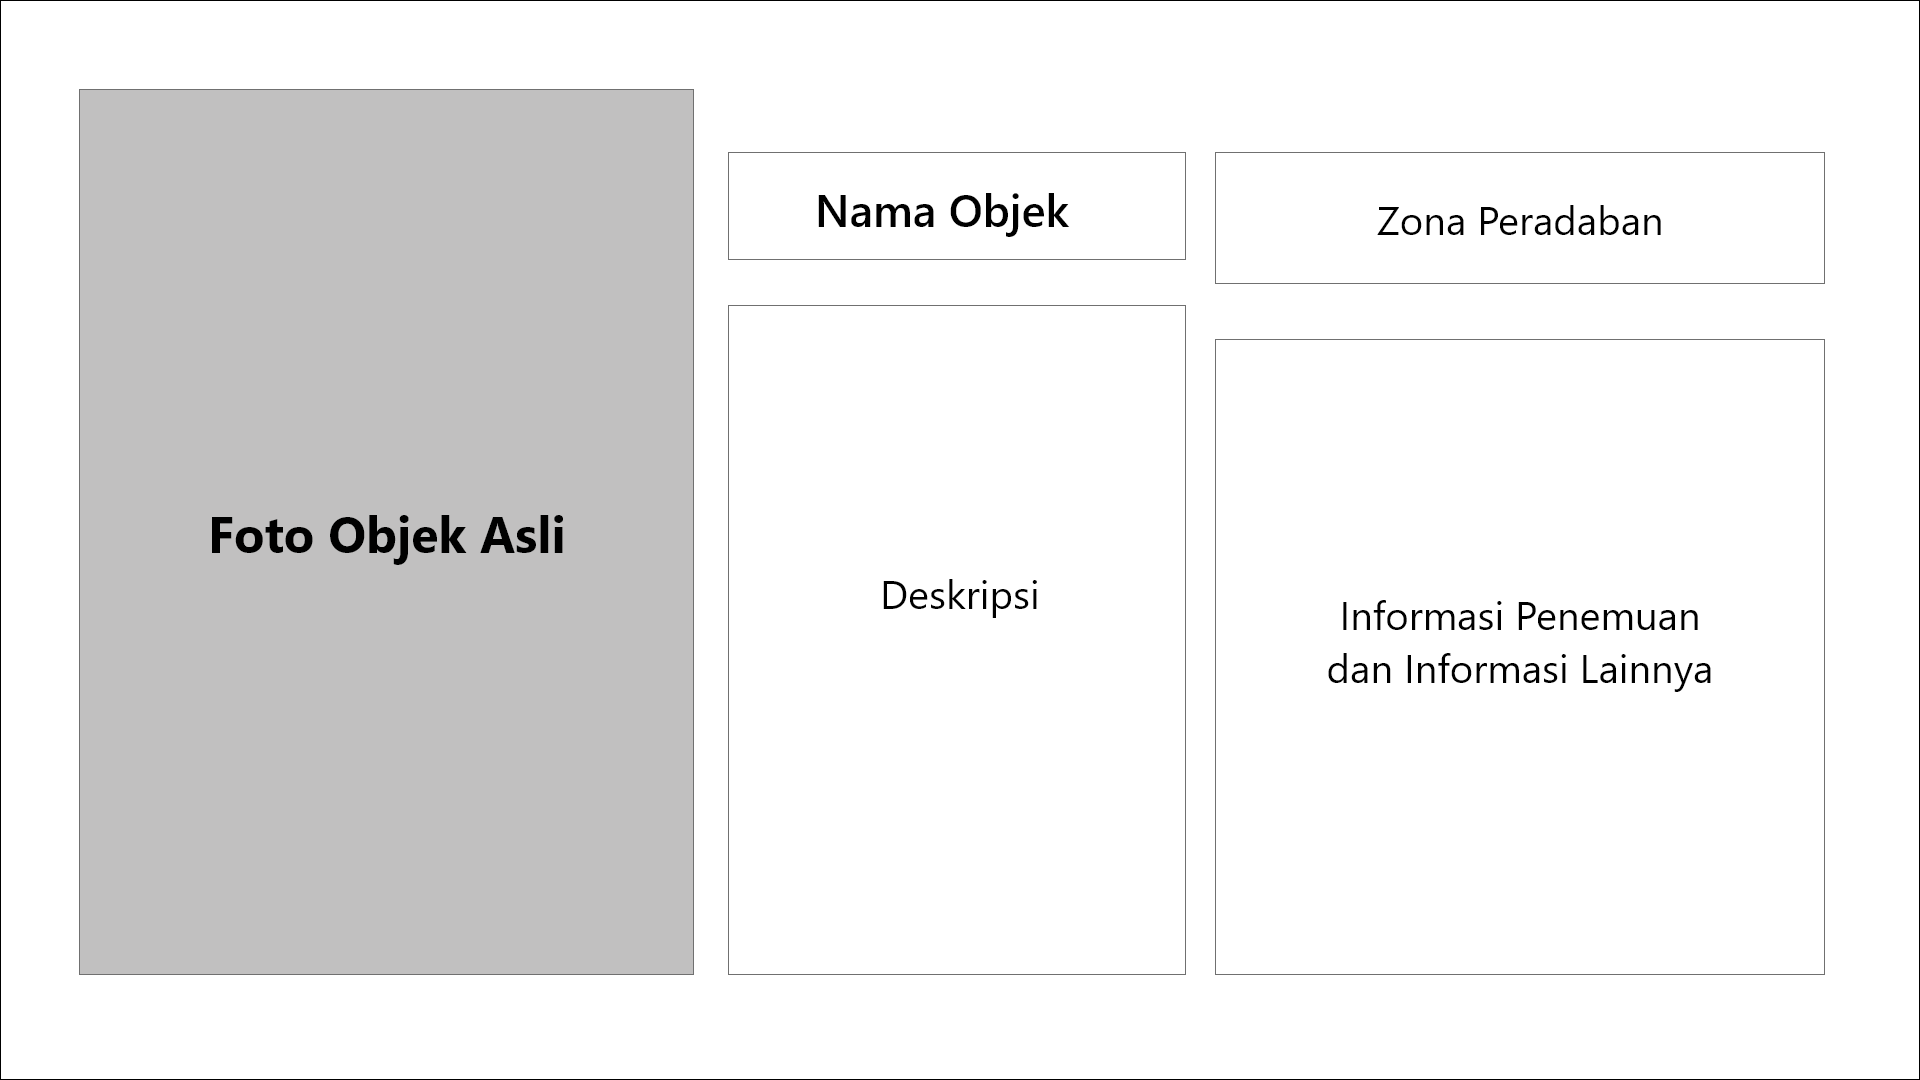
\includegraphics[width=0.6\textwidth]{img/bab3/desain_im.png}}
			\caption{Tampilan utama kedua monitor sistem visualisasi.}
			\label{fig:desain_monitor}
		\end{figure}
		\vspace{-2ex}
		\begin{figure}[H]
			
\includegraphics[width=0.8\textwidth]{img/bab3/storyboard.png}
			\caption{Desain alur menu aplikasi.}
			\label{fig:storyboard}
		\end{figure}
		\vspace{-2ex}
		\begin{figure}[H]
			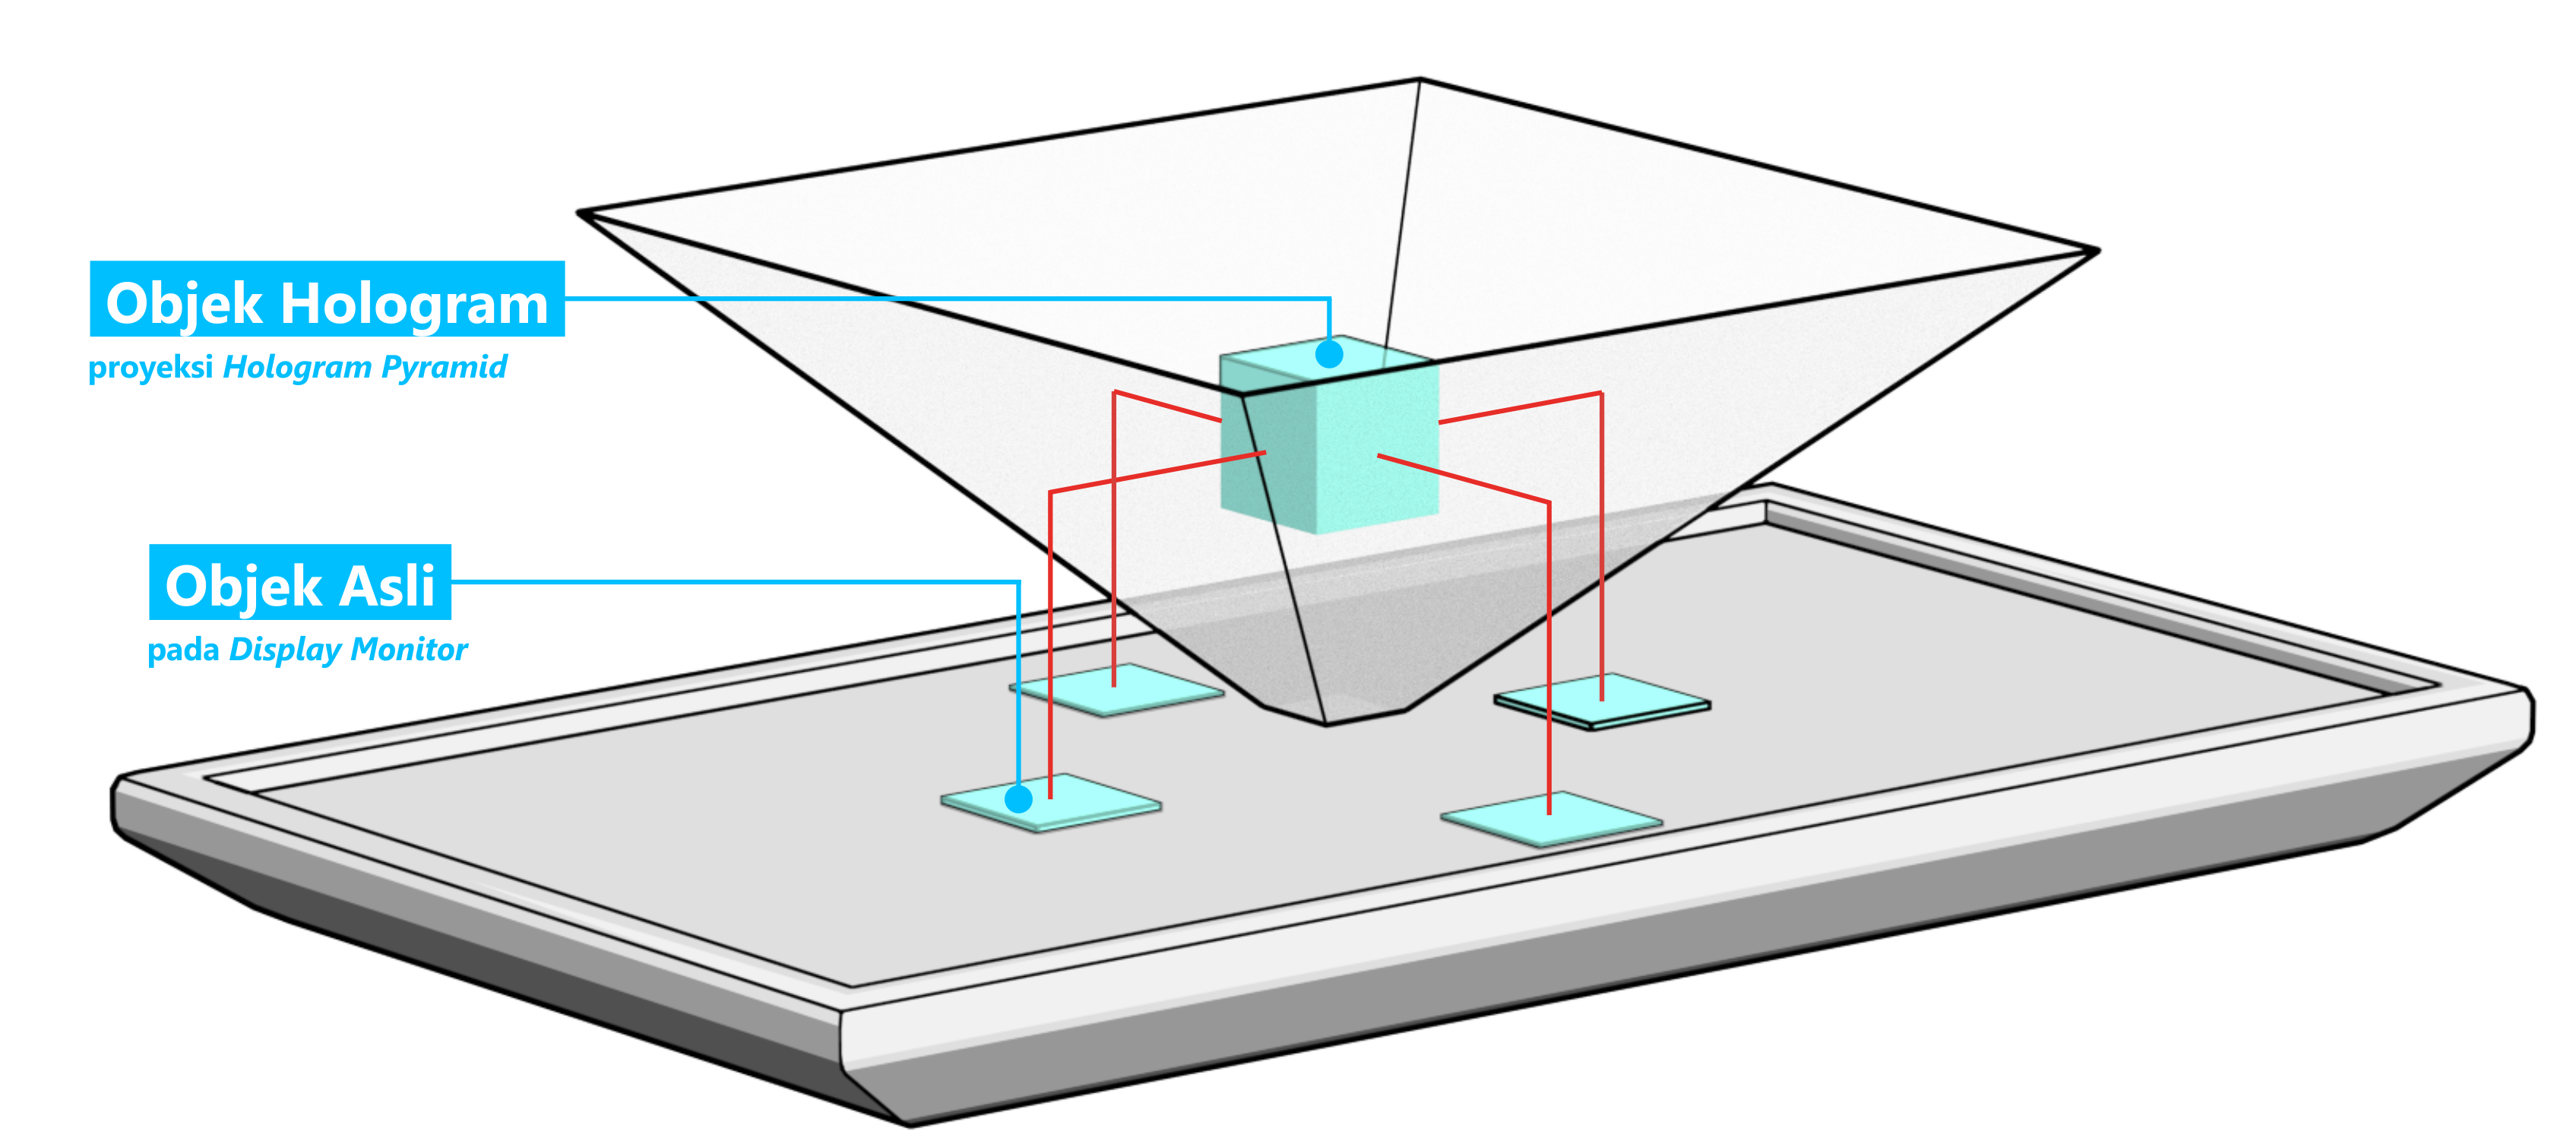
\includegraphics[width=\textwidth]{img/bab3/mekanismehologram.png}
			\caption{Mekanisme \textit{Display Monitor}.}
			\label{fig:proyeksihologram}
		\end{figure}
	\vspace{1.5ex}
	
	\subsection{Desain Sistem Interaksi}
	\vspace{1ex}
		Sistem interaksi yang diterapkan pada penelitian ini menggunakan Leap Motion untuk menangkap \textit{hand gesture} yang diberikan oleh pengguna terhadap objek hologram. Leap Motion bekerja dengan cara mendeteksi adanya pergerakan tangan di dalam jangkauan area pandangnya, kemudian mengirimkan data tersebut ke komputer server untuk diolah dan diambil informasi yang dibutuhkan. Ketika hasil yang diperoleh sesuai dengan fitur yang dibangun, kemudian mengaktifkan respons yang selanjutnya ditunjukkan oleh objek 3D. Alur kerja dari sistem interaksi yang diterapkan ditunjukkan pada gambar \ref{fig:desain_interaksi}.
		\begin{figure} [H]
			
\includegraphics[width=\textwidth]{img/bab3/desain_interaksi.png}
			\caption{Alur kerja sistem interaksi.}
			\label{fig:desain_interaksi}
		\end{figure}
		\vspace{-2ex}
	
		Interaksi yang dapat dilakukan oleh pengguna terhadap sistem visualisasi yang dibangun di antaranya adalah mengeksplorasi objek hologram dan menampilkan menu yang bersesuaian. Fitur-respons yang disediakan berdasarkan \textit{hand gesture} ini ditunjukkan melalui gambar \ref{fig:storyboardgestur}. Semua gestur yang dibangun memiliki ketentuan yang berbeda dalam mengaktifkan respons terkait. Khusus gestur cubitan atau \textit{pinch} untuk mengeksplorasi objek (gambar \ref{fig:gestur2}), gestur \textit{high five} untuk \textit{reset} objek (gambar \ref{fig:gestur4}), gestur \textit{upside} untuk menampilkan menu \textit{Help} (gambar \ref{fig:gestur6}), dan gestur \textit{home} untuk menampilkan \textit{Main Menu} atau keluar dari \textit{Main Scene} (gambar \ref{fig:gestur7}), respons hanya terpanggil jika gestur terdeteksi di kedua tangan secara bersamaan. 
		
		Namun tidak semua gestur membutuhkan kedua tangan (kanan dan kiri) untuk mengaktifkan respons yang bersesuaian. Gestur tersebut di antaranya yaitu gestur genggam atau \textit{punch} (gambar \ref{fig:gestur1}) untuk mengeskplorasi objek, gestur tembak atau \textit{gun} (gambar \ref{fig:gestur3}) untuk mengaktifkan animasi objek, gestur \textit{side thumb} (gambar \ref{fig:gestur5}) untuk mengganti objek yang ditampilkan, dan gestur \textit{thumb up} (gambar \ref{fig:gestur8}) untuk membatalkan atau mengetujui pilihan. Keempatnya pun ada yang dapat mengaktifkan respons jika hanya ada satu gestur di salah satu tangan (kanan atau kiri). 
		
		Meskipun objek hologram dapat dilihat dari seluruh sisi setting perangkat, pengguna hanya dapat berinteraksi di salah satu sisi yang telah dilengkapi dengan \textit{information monitor} dan Leap Motion.
		
		\begin{comment}
		Pada akhirnya \textit{hand model} pada dunia virtual aplikasi akan dimatikan, sehingga menimbulkan kesan seolah-olah pengguna berinteraksi langsung dengan objek hologram dengan tangannya sendiri. 
		\end{comment}
		
		\vspace{-2ex}
		\begin{figure} [H]
			\subfloat[Gestur \textit{punch} untuk eksplorasi objek. \label{fig:gestur1}]{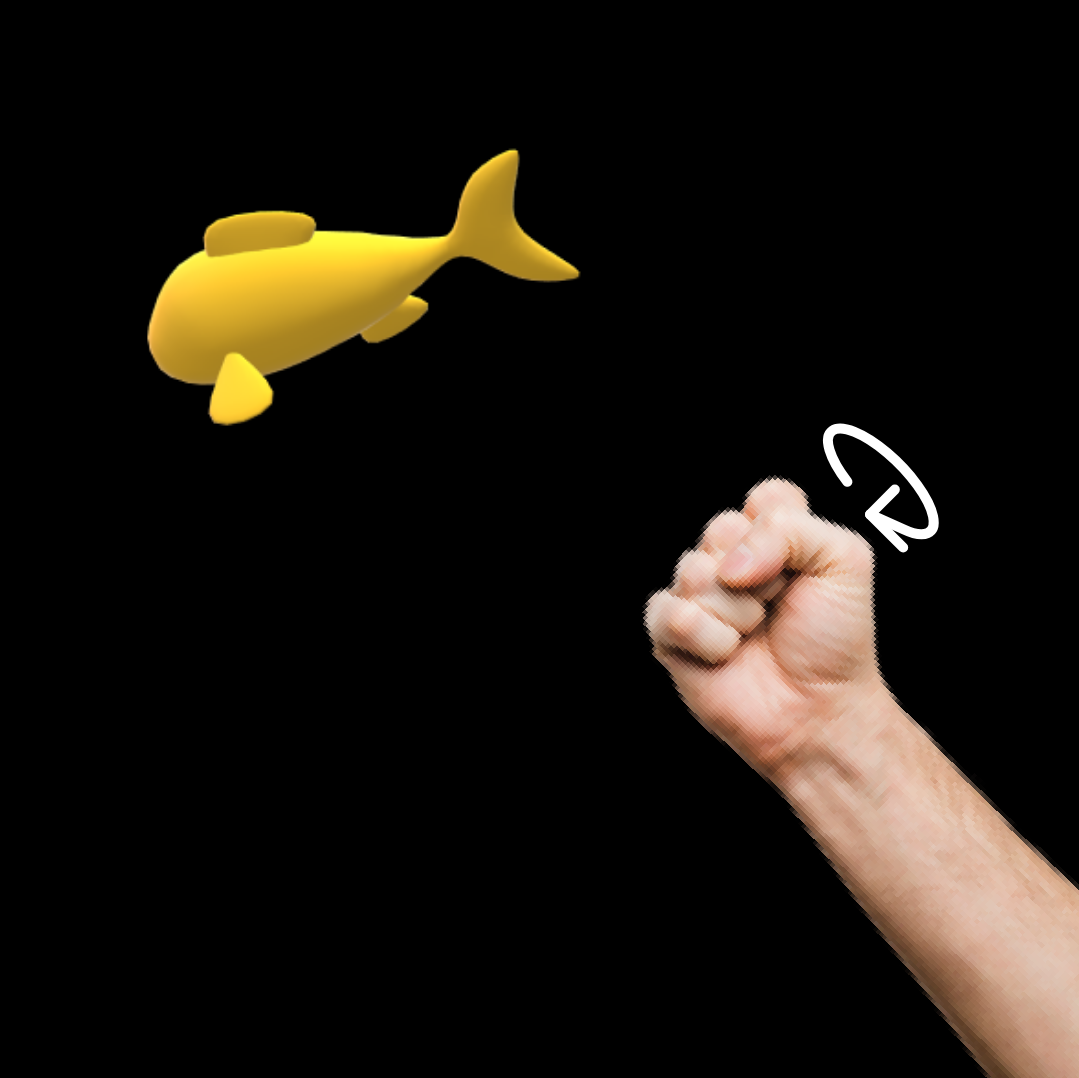
\includegraphics[width=0.32\textwidth]{img/bab3/gestur1.png}}
			\hspace{0.1em}
			\subfloat[Gestur \textit{pinch} untuk zoom objek. \label{fig:gestur2}]{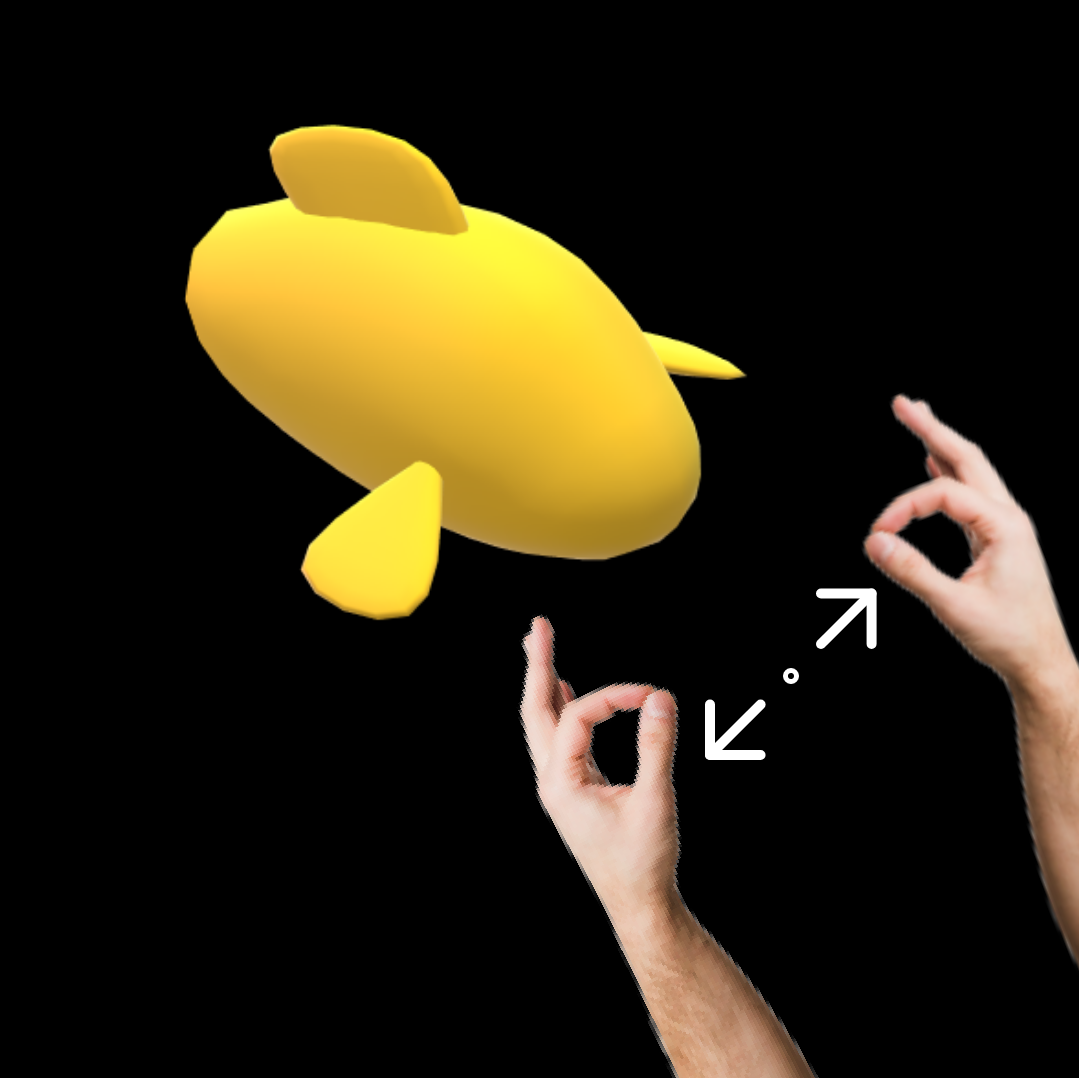
\includegraphics[width=0.32\textwidth]{img/bab3/gestur2.png}}
			\hspace{0.1em}
			\subfloat[Gestur \textit{gun} untuk mengaktifkan animasi. \label{fig:gestur3}]{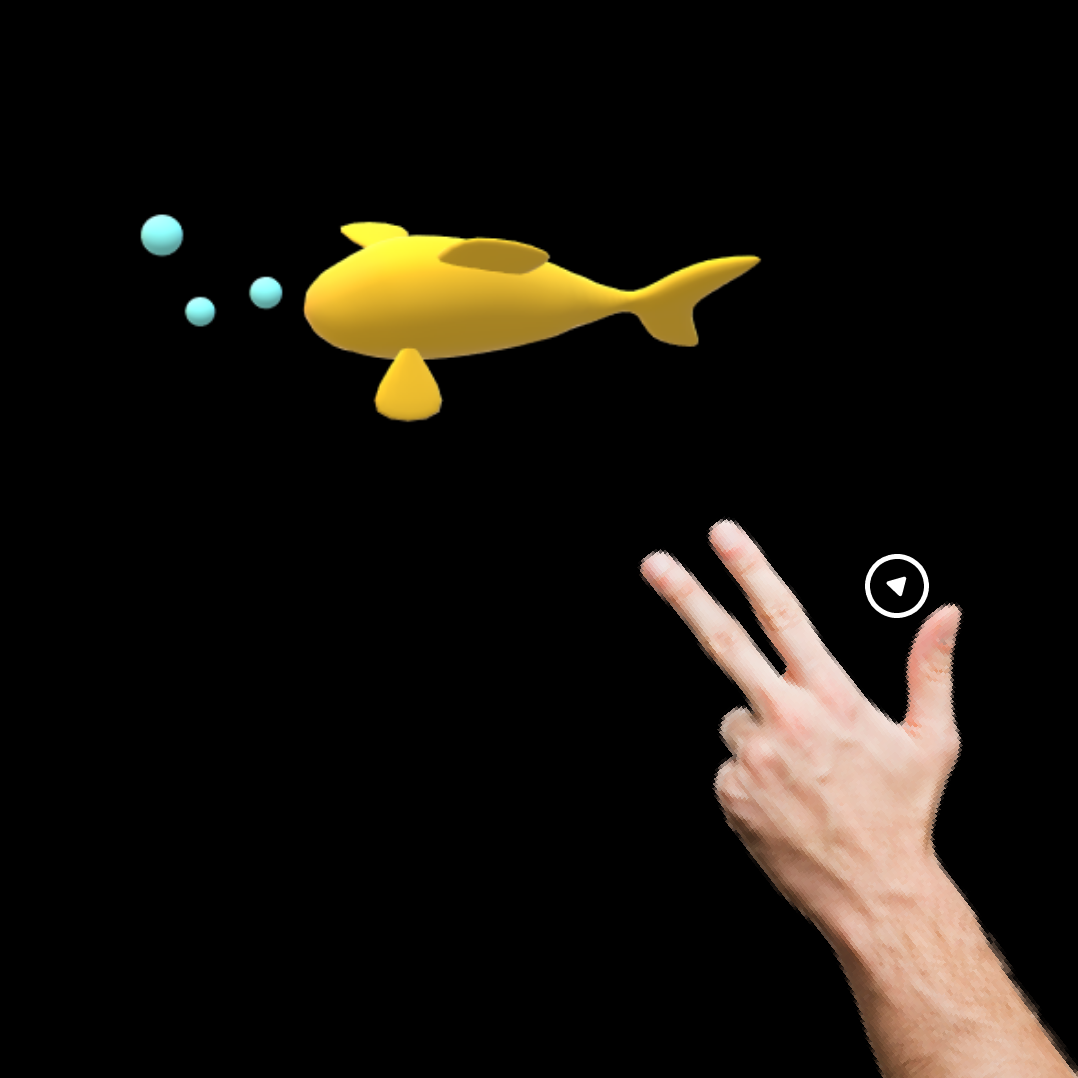
\includegraphics[width=0.32\textwidth]{img/bab3/gestur3.png}}
			\hspace{0.1em}
			\subfloat[Gestur \textit{high five} untuk \textit{reset} objek. \label{fig:gestur4}]{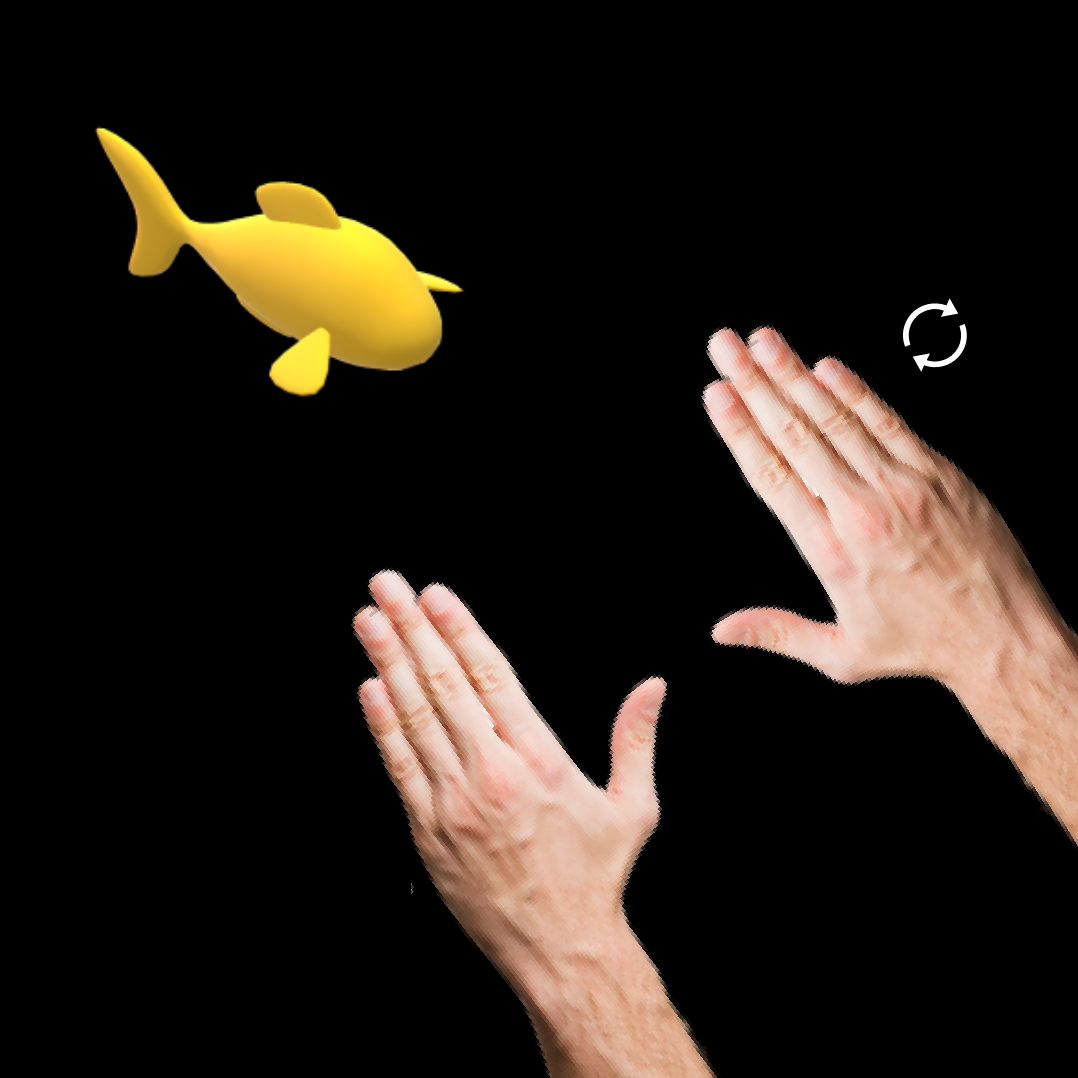
\includegraphics[width=0.32\textwidth]{img/bab3/gestur4.png}}
			\hspace{0.1em}
			\subfloat[Gestur \textit{thumb up} untuk ganti objek. \label{fig:gestur5}]{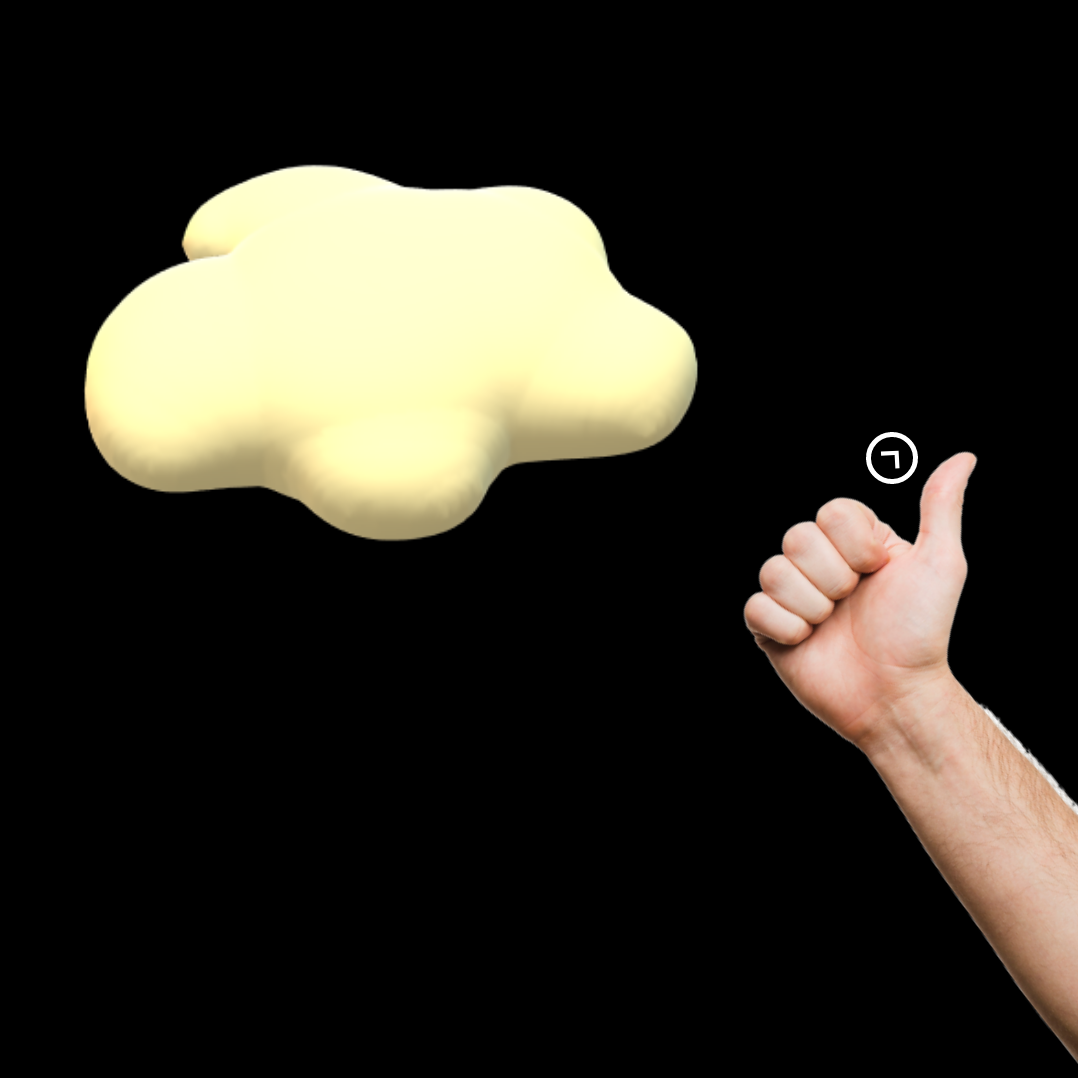
\includegraphics[width=0.32\textwidth]{img/bab3/gestur5.png}}
			\hspace{0.5em}
			\subfloat[Gestur \textit{upside} untuk menampilkan \textit{Help}.
			\label{fig:gestur6}]{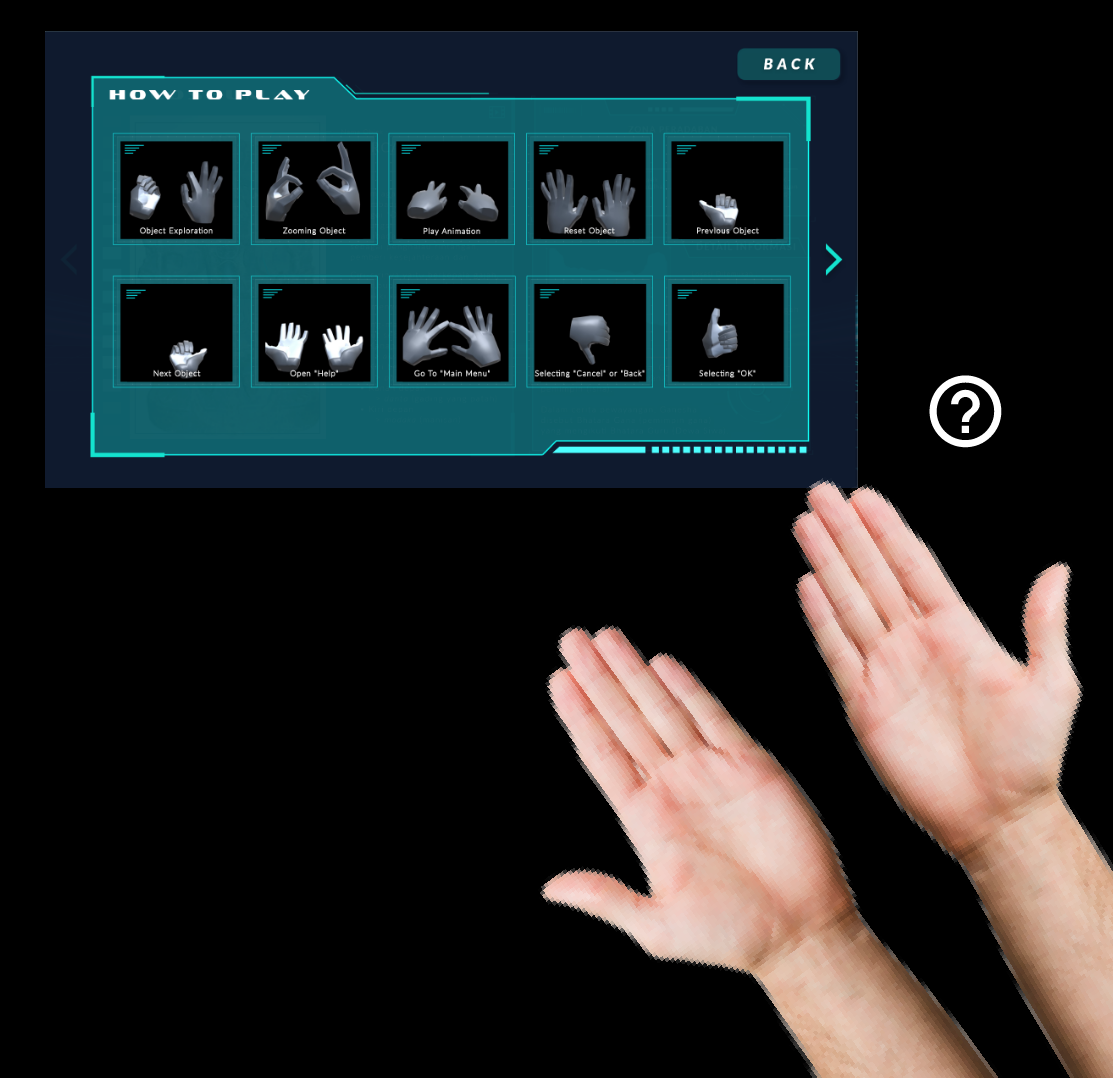
\includegraphics[width=0.32\textwidth]{img/bab3/gestur6.png}}
			\hspace{0.1em}
			\subfloat[Gestur \textit{home} untuk menampilkan \textit{Main Menu}.
			\label{fig:gestur7}]{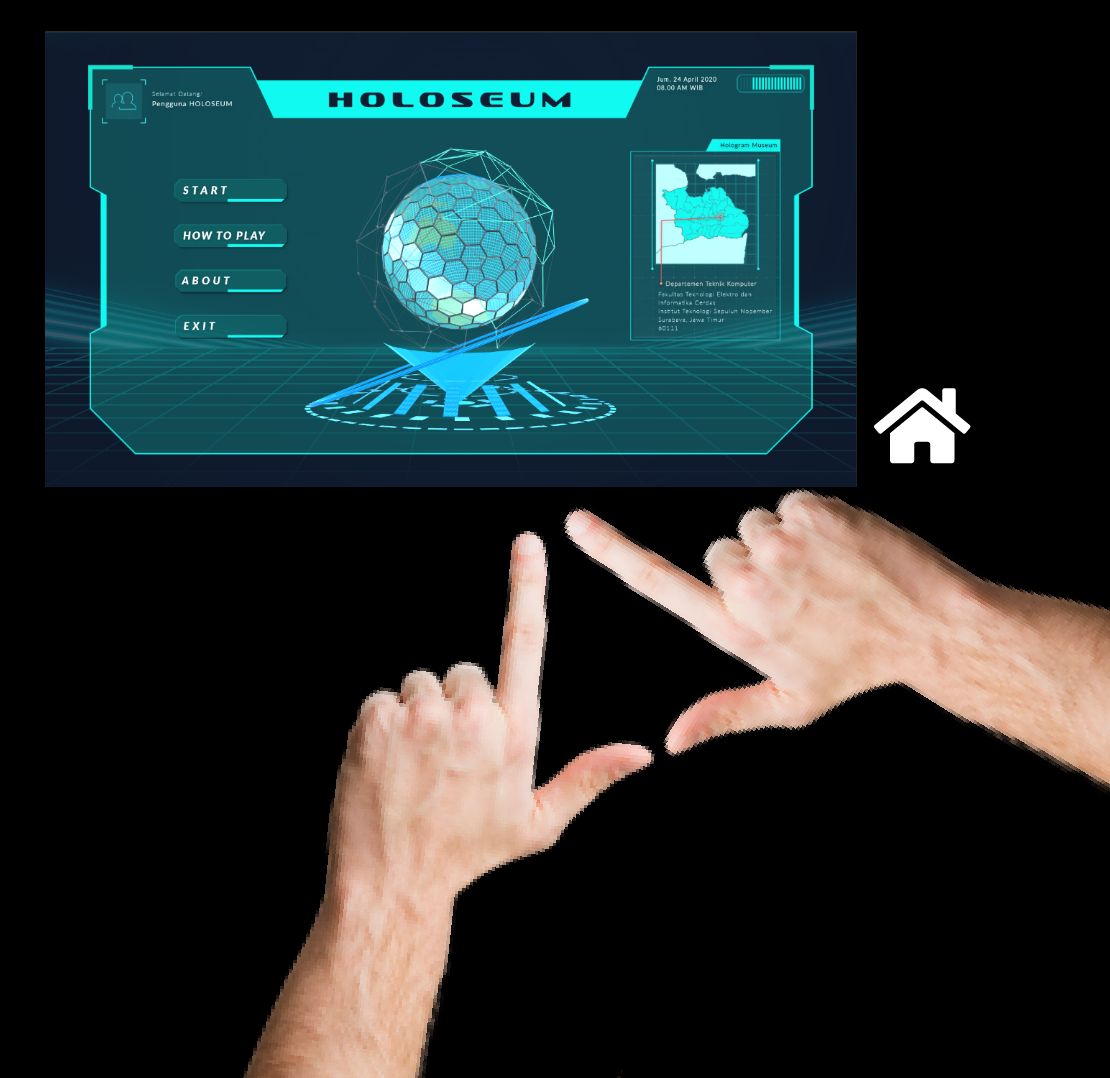
\includegraphics[width=0.32\textwidth]{img/bab3/gestur7.png}}
			\hspace{0.1em}
			\subfloat[Gestur \textit{thumb up} untuk membatalkan dan menyetujui pilihan.
			\label{fig:gestur8}]{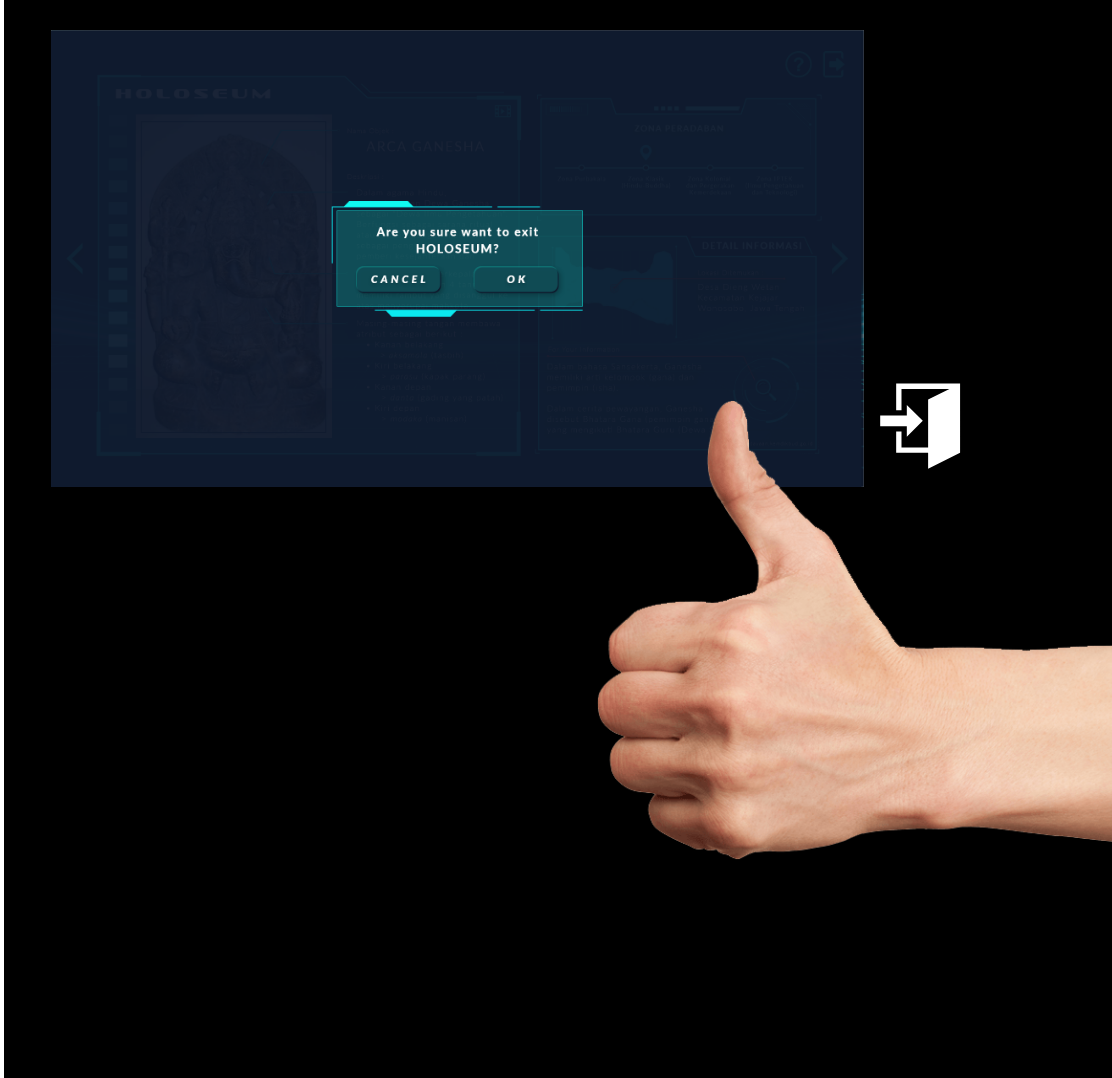
\includegraphics[width=0.32\textwidth]{img/bab3/gestur8.png}}
			\caption{Desain gestur yang membangun sistem interaksi.}
			\label{fig:storyboardgestur}
		\end{figure}
\vspace{2ex}

\section{Alur Implementasi Sistem}
\vspace{1ex}
	Alur implementasi dalam pengerjaan penelitian Tugas Akhir ini dapat dibagi menjadi beberapa tahapan sebagai penunjang dalam menjalankan penelitian.
	\begin{figure} [H]
		
\includegraphics[width=\textwidth]{img/bab3/metodologi.png}
		\caption{Alur implementasi penelitian.}
		\label{fig:metodologi}
	\end{figure}

	Alur implementasi yang dilakukan dapat diuraikan secara sederhana pada gambar \ref{fig:metodologi} dan dapat dijelaskan sebagai berikut :
	\begin{enumerate} [nolistsep]
		\item \textbf{Desain Sistem Keseluruhan}.
		
		Perancangan ini berkaitan dengan keseluruhan sistem yang dibutuhkan, dari \textit{storyboard} penggunaan dan setting perangkat, visualisasi hologram 3D dan penampilan informasi, hingga interaksi antara pengguna dan objek hologram.
		
		\item \textbf{Pembuatan Sitem Visualisasi}.
		
		Pada tahap ini dilakukan pengumpulkan asset objek 3D yang dibutuhkan. Modifikasi dan penyesuaian objek 3D diperlukan agar siap diprogram dan ditampilkan dalam bentuk \textit{hologram video}. \textit{Interface} aplikasi juga direalisasikan di tahap ini.
		
		\item \textbf{Pembuatan Setting Perangkat}.
		
		\textit{Hologram video} yang dibuat diproyeksikan melalui \textit{pyramid hologram}. Berdasarkan desain yang direncanakan, maka dibuat dan disusun setting perangkatnya agar mampu menjalankan keseluruhan sistem.
		
		\item \textbf{Pembuatan Sistem Interaksi}.
		
		Objek hologram yang terbentuk dapat digerakkan oleh pengguna berdasarkan \textit{hand gesture} menggunakan Leap Motion. Untuk memahami \textit{hand gesture} yang diberikan, fitur tersebut dirancang dan direalisasikan pada tahap ini.
		
		\item \textbf{Integrasi Sistem Visualisasi dan Interaksi}.
		
		Pada tahap ini sistem visualisasi dan interaksi digabungkan pada set yang telah dirancang. Objek hologram yang ditampilkan dapat merespons gerakan pengguna sesuai dengan fitur yang diterapkan.
		
		\item \textbf{Pengujian Sistem}.
		
		Pengujian sistem dilakukan untuk mendapatkan hasil dari implementasi alat yang digunakan sebagai bahan evaluasi dan pengembangan selanjutnya. 
	\end{enumerate}
\vspace{2ex}
	


\section{Implementasi Setting Perangkat}
\vspace{1ex}
	Setting perangkat yang dirancang dibangun menggunakan bahan dasar multiplex (10mm dan 3mm). Setting perangkat yang direncanakan tidak dapat diselesaikan secara keseluruhan, hanya bagian penompang \textit{display monitor} saja yang berhasil dirakit. Akibat keadaan yang tidak stabil, pembuatan setting perangkat tidak dapat dilanjutkan. Maka dibentuklah setting sesuai yang ditampilkan pada gambar \ref{fig:foto_alat}. \textit{Server Computer} yang digunakan yaitu Asus ROG Strix GL553VD. \textit{Display monitor} yang digunakan adalah Acer X193HQ berukuran 18.5 inch (23 x 41 cm) dengan \textit{pyramid hologram} berukuran 24 x 24 x 12 cm berbahan akrilik transparan 2 mm. Peletakkan \textit{display monitor} dan \textit{pyramid hologram} ditukar sehingga \textit{display monitor} yang terletak di bawah menopang \textit{pyramid hologram} yang terbuka ke atas sesuai pada gambar \ref{fig:proyeksihologram}. Leap Motion diletakkan di depan salah satu sisi. Ukuran ideal dari objek hologram yang dapat ditampilkan adalah sebesar 3 x 3 x 3 cm (1/7.8 dari lebar monitor). Pengujian dilakukan sebagaimana yang akan diterapkan pada desain setting perangkat awal. 
	\begin{figure} [H]
		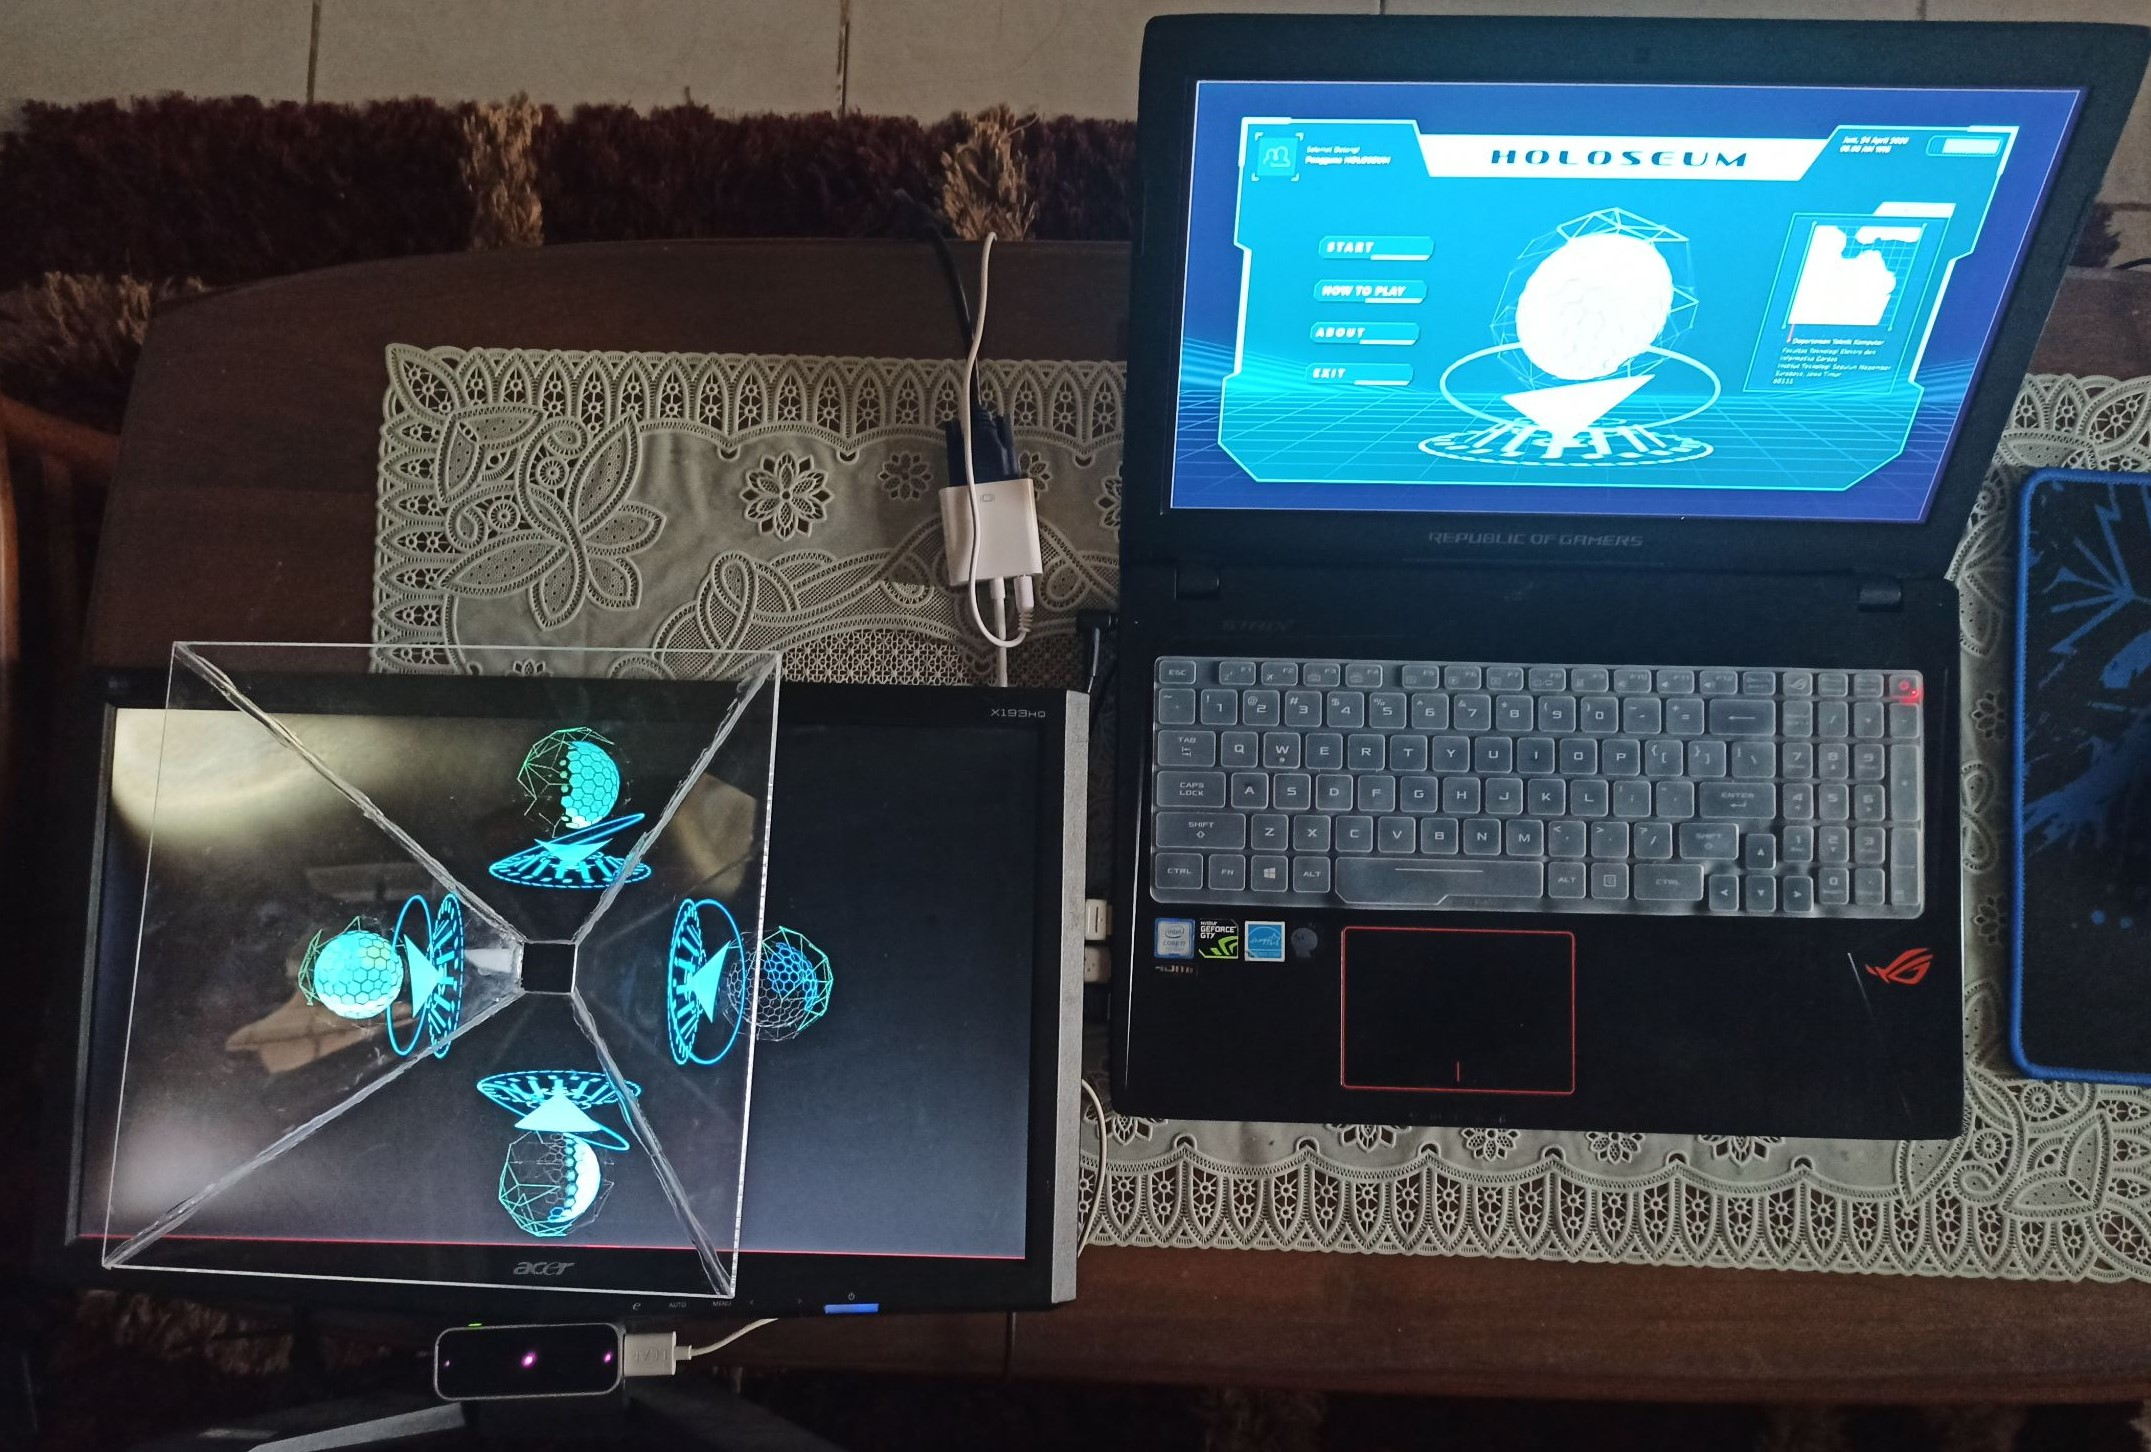
\includegraphics[width=0.8\textwidth]{img/bab3/foto_alat.jpg}
		\caption{Setting perangkat yang dibangun.}
		\label{fig:foto_alat}
	\end{figure}
\vspace{2ex}

\section{Implementasi Sistem Visualisasi} \label{section:visualisasi}
\vspace{1ex}
	Sistem visualisasi dibangun dengan memanfaatkan \textit{engine} Unity 2018.4.17f1. Dalam merealisasikan penelitian ini, digunakan dua monitor untuk menampilkan \textit{hologram video} dari objek hologram oleh \textit{display monitor} dan menampilkan menu aplikasi oleh \textit{information monitor}. Keduanya diprogram untuk dapat berjalan secara paralel.
\vspace{1.5ex}
	
	\subsection{Penyesuaian Objek Hologram}
	\vspace{1ex}
		Objek-objek berupa koleksi museum diperoleh dari asset 3D yang telah disediakan maupun hasil eksplorasi dari Sketchfab dengan referensi tertulis. Objek yang digunakan ditunjukkan pada gambar \ref{fig:objek3d}. Tabel \ref{fig:info_objek} menunjukkan informasi dari jumlah \textit{vertex} dan \textit{poly} objek 3D tersebut.
		\begin{figure} [H]
			\subfloat[\textit{Hand Axe}\cite{handaxe}.]{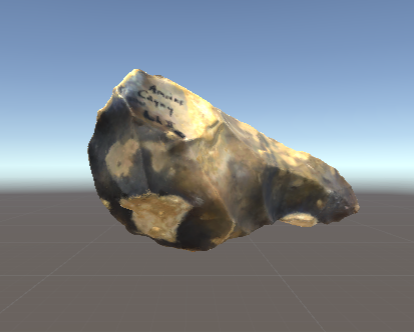
\includegraphics[width=0.32\textwidth]{img/obj/obj1_a.png}}
			\hspace{0.1em}
			\subfloat[\textit{Primeval Axe}\cite{primeval}.]{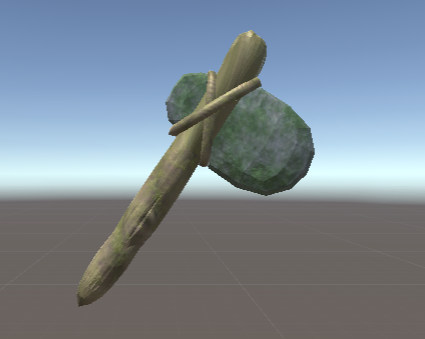
\includegraphics[width=0.32\textwidth]{img/obj/obj2_a.png}}
			\hspace{0.1em}
			\subfloat[\textit{Buddha Statue}\cite{buddha_lowpoly}.]{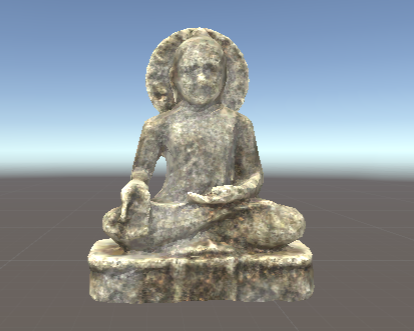
\includegraphics[width=0.32\textwidth]{img/obj/obj3_a.png}}
			\hspace{0.1em}
			\subfloat[\textit{Ganesha Statue}\cite{ganesha}.]{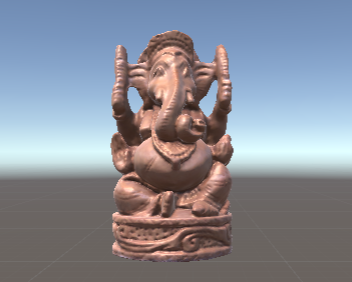
\includegraphics[width=0.32\textwidth]{img/obj/obj4_a.png}}
			\hspace{0.1em}
			\subfloat[\textit{Brass Lamp}\cite{brasslamp}.]{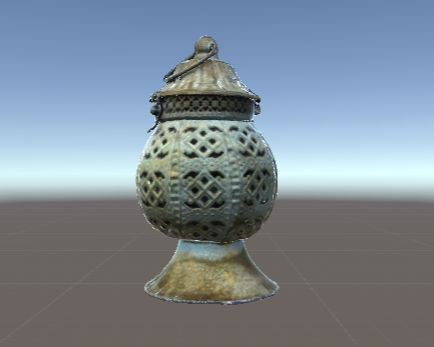
\includegraphics[width=0.32\textwidth]{img/obj/obj5_a.png}}
			\hspace{0.1em}
			\subfloat[\textit{Ceramic Pot}\cite{ceramicpot}.]{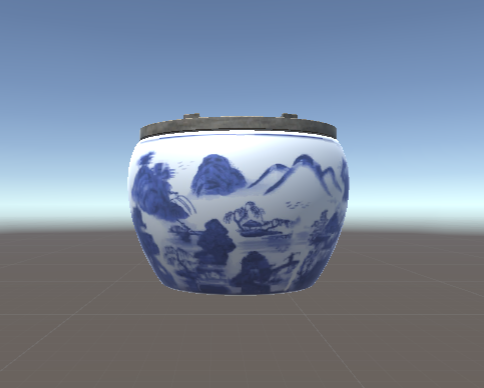
\includegraphics[width=0.32\textwidth]{img/obj/obj6_a.png}}
			\hspace{0.1em}
			\subfloat[\textit{Typewriter}\cite{typewriter}.]{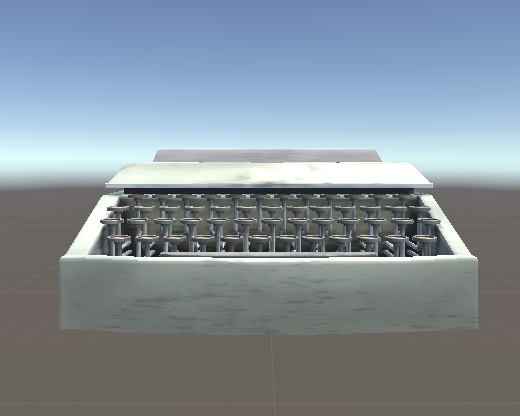
\includegraphics[width=0.32\textwidth]{img/obj/obj7_aa.png}}
			\hspace{0.1em}
			\subfloat[\textit{Gramophone}.]{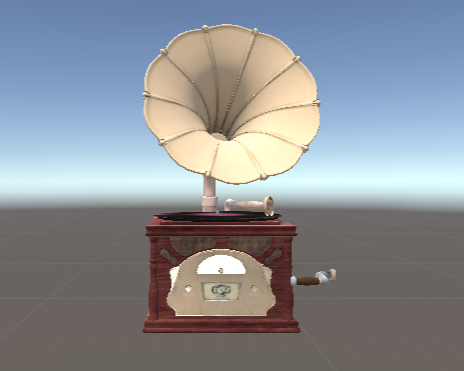
\includegraphics[width=0.32\textwidth]{img/obj/obj8_a.png}}
			\caption{Objek 3D yang digunakan pada penelitian.}
			\label{fig:objek3d}
		\end{figure}
		\vspace{-2ex}
	
		\begin{table}[H]
			\caption{Informasi jumlah \textit{poly} dan \textit{vertex} setiap objek 3D.}
			\label{fig:info_objek}
			\begin{tabular}{|c|l|L{2.5cm}|c|c|}
				\hline
				\textbf{No} & \multicolumn{1}{c|}{\textbf{Nama Objek}} & \multicolumn{1}{c|}{\textbf{Zona Peradaban}} & \textbf{\textit{Poly}} & \textbf{\textit{Vertex}} \\ \hline
				1.& \textit{Hand Axe}      & Purbakala            & 60000 & 30002  \\ \hline
				2.& \textit{Primeval Axe}  & Purbakala            & 1585  & 1180   \\ \hline
				3.& \textit{Buddha Statue} & Klasik 				 & 3000  & 1512   \\ \hline
				4.& \textit{Ganesha Statue}& Klasik 				 & 29124 & 14558  \\ \hline
				5.& \textit{Brass Lamp}    & Kolonial             & 27300 & 13640  \\ \hline
				6.& \textit{Ceramic Pot}   & Kolonial             & 1510  & 1522   \\ \hline
				7.& \textit{Typewriter}    & IPTEK                & 19218 & 18387   \\ \hline
				8.& \textit{Gramophone}    & IPTEK                & 17837 & 18682  \\ \hline
			\end{tabular}
		\end{table}
	
		Objek 3D yang diperoleh tidak dapat langsung direkonstruksi menjadi \textit{hologram video}, melainkan harus melalui proses penyesuaian terlebih dahulu. Pada dasarnya, penyesuaian ini terjadi melalui 2 proses menggunakan \textit{engine} yang berbeda. Untuk memodifikasi detail objek berdasarkan elemen penyusunnya, maka memerlukan aplikasi \textit{3D modelling} berupa Autodesk 3ds Max 2017. Contohnya untuk menambah atau mengurangi suatu elemen dalam objek tersebut seperti pada gambar \ref{fig:3dsmax}. Kemudian memindahkan titik poros objek pada posisi 0,0,0 yang ditunjukkan pada gambar \ref{fig:3dsmaxb} dengan tujuan agar objek hologram yang diinteraksikan seimbang tanpa terpotong \textit{workspace} yang dijelaskan lebih lengkap melalui \nameref{section:porosobjek}.
		\vspace{-2ex}
		\begin{figure} [H]
			\subfloat[Objek sebelum modifikasi\cite{buddha_lowpoly}.]{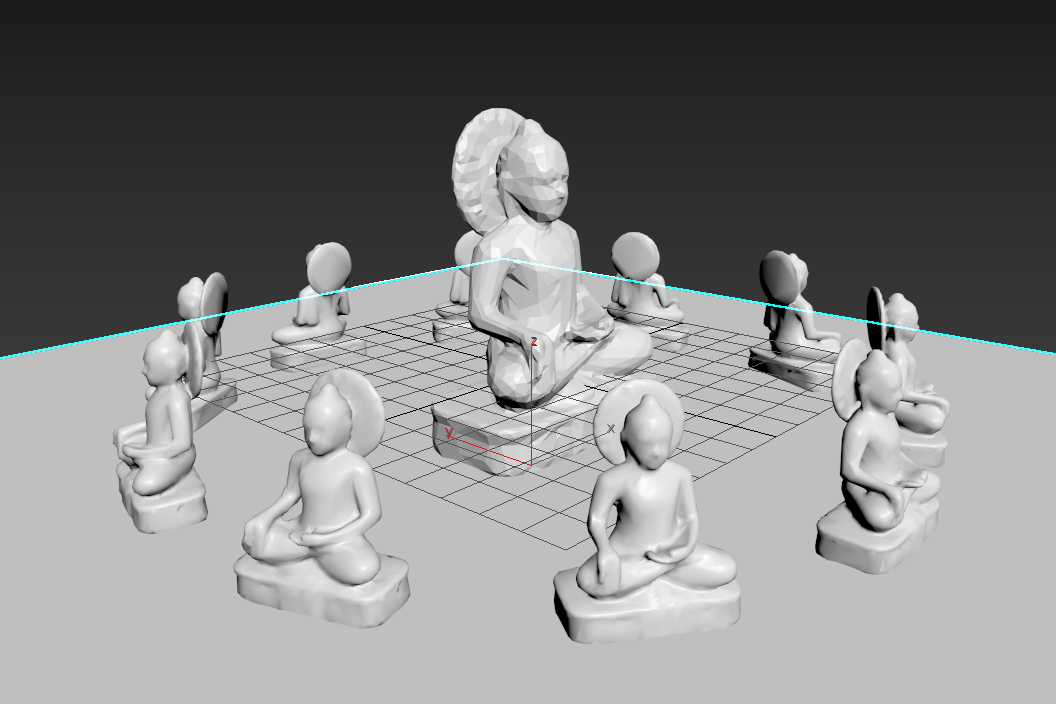
\includegraphics[width=0.47\textwidth]{img/bab3/buddha_banyak.png}}
			\hspace{0.1em}
			\subfloat[Objek setelah modifikasi.\label{fig:3dsmaxb}]{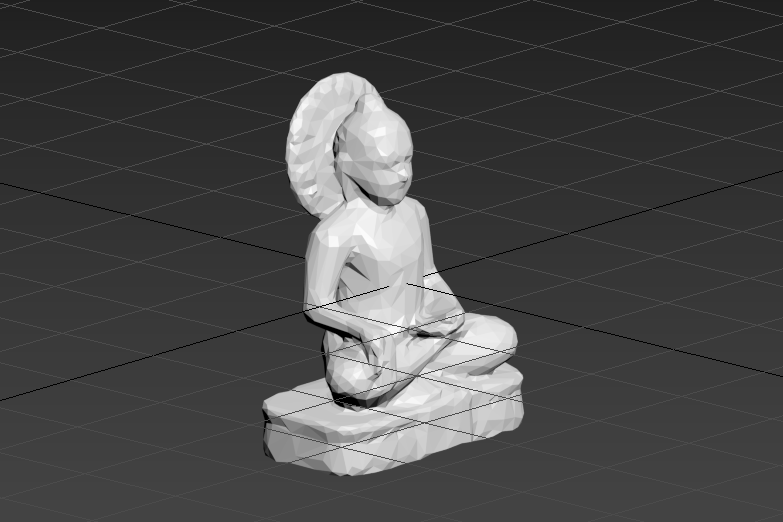
\includegraphics[width=0.47\textwidth]{img/bab3/buddha_1.png}}
			\caption{Penyesuaian objek pada Autodesk 3ds Max 2017.}
			\label{fig:3dsmax}
		\end{figure}
		\vspace{-2ex}
		
		Penyesuaian kedua menggunakan \textit{engine} Unity bertujuan mengatur objek dan membangun fitur pelengkap sebelum direkonstruksi menjadi \textit{hologram video}. Objek yang telah di-\textit{import} diatur posisi utama di tengah \textit{camera setting} dan disesuaikan ukurannya menggunakan \textit{scale}. Hubungan antara pengaturan posisi objek dan kamera akan dijelaskan pada bagian \nameref{section:rekonstruksi}. Setiap objek harus dipastikan telah melalui proses \nameref{section:standard} dan dilengkapi dengan komponen  \textit{collider} dan \textit{rigidbody}. \textit{Collider} berfungsi untuk memadatkan objek sehingga objek yang saling bertabrakan tidak akan saling menembus. Dalam penelitian ini, \textit{collider} dimanfaatkan untuk membuat \textit{workspace area} pergerakan objek 3D pada bagian \nameref{section:workspace}. Sedangkan \textit{rigidbody} berfungsi untuk memberikan efek gravitasi pada suatu objek, dimana jika ada gaya yang diberikan pada objek maka objek dapat 'merasakan' dan memberikan \textit{feedback}. Dalam penelitian ini, \textit{rigidbody} dimanfaatkan agar objek 3D dapat "melayang" pada \textit{workspace} yang dibangun. Pengaturan ini juga memungkinkan objek 3D dapat berputar (rotasi) dan bergerak dalam \textit{workspace area}. Pengaturan \textit{collider} dan \textit{rigidbody} ditunjukkan pada gambar \ref{fig:unity_colgid}. Penyesuaian pada tahap ini juga dimanfaatkan untuk membangun fitur respons berdasarkan gestur yang dimasukkan, seperti faktor pengali atau \textit{scale} untuk membangun fitur \textit{zoom} dan pengaturan posisi beserta rotasi dalam membangun fitur \textit{reset to default}. Selengkapnya dijelaskan pada bagian \nameref{section:implementasi_interaksi}. Sedangkan untuk memberikan efek hologram, maka yang harus diatur adalah material dan \textit{shader} yang membangun objek tersebut. Penyesuaian untuk memberikan efek hologram dilakukan hingga mencapai efek yang dihendaki. Selain itu, penyesuaian di Unity juga dapat dimanfaatkan untuk menciptakan animasi dengan memindah, memutar, atau mengatur ukuran komponennya.
		\begin{figure} [H]
			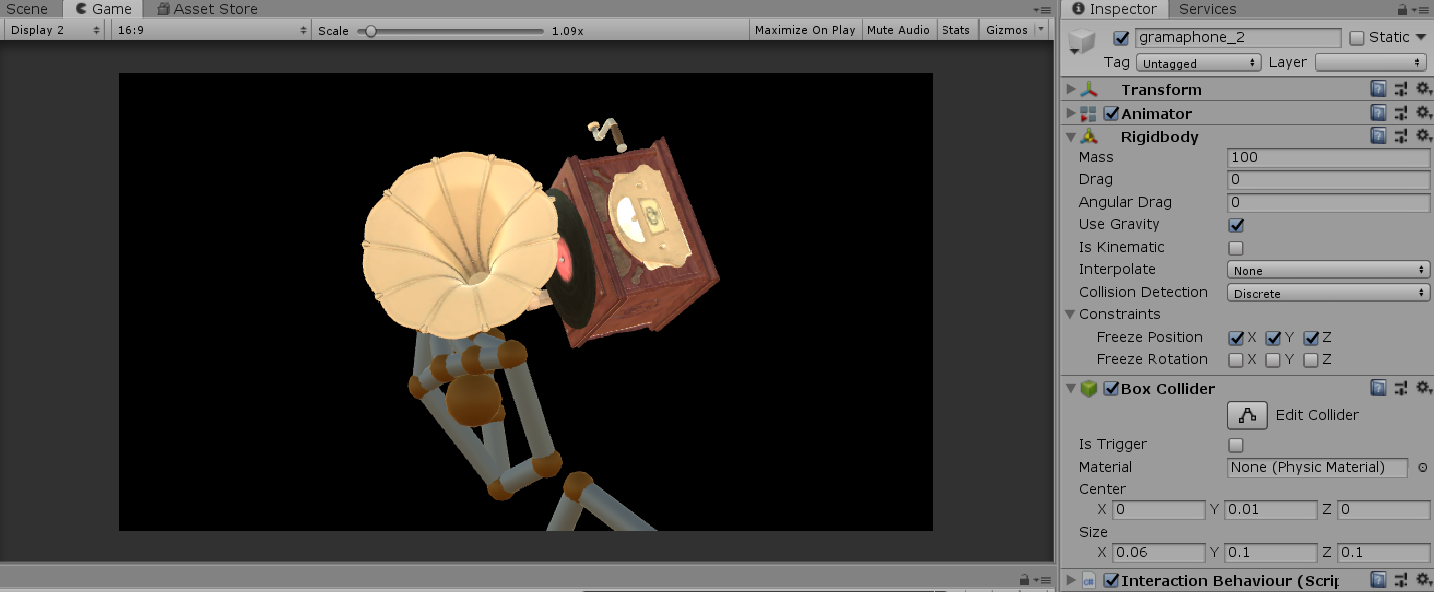
\includegraphics[width=0.9\textwidth]{img/bab3/unity_colgid.png}
			\caption{Penyesuaian melalui \textit{collider} dan \textit{rigidbody} pada Unity.}
			\label{fig:unity_colgid}
		\end{figure}
		\begin{comment}
		Sedangkan untuk memberikan efek hologram, maka yang harus diatur adalah material dan \textit{shader} yang membangun objek tersebut. Material pada Unity disediakan oleh \textit{shader Standard} dan \textit{shader Standard Specular Setup} (gambar \ref{fig:unity_material}). \textit{Specular Setup} langsung mengatur tingkat kecerahan dari specularnya langsung, sedangkan \textit{Metallic Setup} pada \textit{shader Standard} harus mengatur parameter lain dan efek specularnya muncul karena perubahan itu\cite{unity_spec}. Penyesuaian untuk memberikan efek hologram dilakukan hingga mencapai efek yang dihendaki.
		\begin{figure} [H]
			\subfloat[\textit{Shader Standard}.]{\includegraphics[width=0.47\textwidth]{img/bab3/standard.png}}
			\hspace{0.1em}
			\subfloat[\textit{Shader Standard Specular}.]{\includegraphics[width=0.47\textwidth]{img/bab3/standard_specular.png}}
			\caption{Perbedaan material \textit{shader} pada Unity.}
			\label{fig:unity_material}
		\end{figure}
		\end{comment}
				\vspace{1ex}
		
		\subsubsection{Penyesuaian Titik Poros Objek} \label{section:porosobjek}
		\vspace{0.5ex}
			\begin{figure} [!h]
				\subfloat[Titik poros asli objek pada Autodesk 3ds Max 2017.\label{fig:000bawah}]{\includegraphics[width=0.47\textwidth]{img/bab3/000bawah.png}}
				\hspace{0.1em}
				\subfloat[Titik poros objek baru pada Autodesk 3ds Max 2017.\label{fig:000tengah}]{\includegraphics[width=0.47\textwidth]{img/bab3/000tengah.png}}
				\hspace{0.1em}
				\subfloat[Titik poros asli objek pada Unity.\label{fig:000bawah_unity}]{\includegraphics[width=0.47\textwidth]{img/bab3/000bawah_unity.png}}
				\hspace{0.1em}
				\subfloat[Titik poros objek baru pada Unity.\label{fig:000tengah_unity}]{\includegraphics[width=0.47\textwidth]{img/bab3/000tengah_unity.png}}
				\hspace{0.1em}
				\subfloat[Objek dengan titik poros asli pada saat diputar.\label{fig:000bawah_unity2}]{\includegraphics[width=0.47\textwidth]{img/bab3/000bawah_unity2.png}}
				\hspace{0.1em}
				\subfloat[Objek dengan titik poros baru pada saat diputar.\label{fig:000tengah_unity2}]{\includegraphics[width=0.47\textwidth]{img/bab3/000tengah_unity2.png}}
				\caption{Efek pemindahan titik poros objek.}
				\label{fig:pindahporos}
			\end{figure}
			
			%kenapa harus dipindah
			Setiap objek memiliki titik poros yang berbeda dikarenakan titik poros ditentukan oleh 3D \textit{artist} yang membuat objek 3D tersebut yang bebas diletakkan dimana saja. Pemindahan ini bertujuan untuk menyeragamkan titik poros dari seluruh objek 3D yang digunakan. Perbedaan titik poros tiap objek yang digunakan mempengaruhi perspektif antara pengguna dan objek khususnya pada proses rotasi objek. Rotasi memerlukan titik poros perputaran sehingga untuk membuat objek dapat berputar dengan seimbang pada workspace yang ditentukan, maka titik poros objek harus diletakkan tepat pada tengah objek tersebut. Pada penelitian ini, rotasi objek 3d dilakukan berdasarkan pergerakan tangan (lihat \nameref{section:eksplorasi}) sehingga dibutuhkan orientasi yang sama antara objek dengan tangan pengguna. Efek dari pemindahan titik poros objek ditunjukkan pada gambar \ref{fig:pindahporos}. Pada gambar \ref{fig:000bawah}, objek asli memiliki titik poros pada tengah di bawah objek sehingga jika diputar maka menghasilkan gambar \ref{fig:000bawah_unity2} dimana ada bagian yang terpotong workspace saat dirotasikan. Sedangkan pada gambar \ref{fig:000tengah} saat titik poros objek dipindahkan  tepat pada tengah objek, sehingga saat diputar maka menghasilkan gambar \ref{fig:000tengah_unity2} dimana perputarannya lebih seimbang tanpa memotong objek yang ditampilkan pada pengguna.
			
			%kenapa dipindahnya ke 0,0,0
			Titik poros objek dipindah ke 0,0,0 agar saat di import ke Unity, penempatan objek sesuai dengan inisialisasi \textit{transform} pada Unity. Saat titik poros tidak tepat pada tengah objek di titik 0,0,0 sesuai gambar \ref{fig:000bawah}, maka selisih antara titik poros asli dengan titik tengah seharusnya akan memengaruhi \textit{transform} pada Unity yang ditunjukkan pada gambar \ref{fig:000bawah_unity}. Sedangkan jika titik poros objek tepat di tengah objek pada posisi 0,0,0 sesuai gambar \ref{fig:000tengah}, maka tidak ada selisih yang menyebabkan posisi objek dapat diatur langsung melalui \textit{transform} Unity sehingga objek tetap berada di tengah dan tetap seimbang seperti gambar  \ref{fig:000tengah_unity}. Objek diletakkan tepat di titik 0,0,0 pada Unity yang menjadi titik fokus pandangan pengguna.
		\vspace{0.75ex}
		
		\subsubsection{Pengaturan Nilai Standard Objek} \label{section:standard}
		\vspace{0.5ex}
			Setiap objek memiliki standard yang berbeda-beda dikarenakan nilai perhitungan yang bebeda pula. Pada penelitian ini, standard objek yang harus didefinisikan terlebih dahulu di antaranya nilai posisi awal, nilai rotasi awal, nilai minimum dan maksimum perbesaran yang ditunjukkan pada gambar \ref{fig:eachobject}. Khusus untuk nilai minimum dan maksimum \textit{workspace area} dijelaskan pada \nameref{section:workspace}. Pendefinisian ini bermanfaat untuk mengembalikan objek pada keadaan awal pada \textit{reset to default} dan mendapatkan nilai perhitungan ukuran objek pada \textit{zoom object}. Hal ini dikarenakan pada setiap pergantian frame, nilai posisi, rotasi, dan ukuran objek selalu diperbarui. Untuk posisi dan rotasi objek, objek berpindah dan berputar saat eksplorasi atau \textit{reset to default} dilakukan selama berada dalam \textit{workspace area} yang didefinisikan seperti pada flowchart \ref{fig:standard_pr}. Sedangkan ukuran objek, objek akan berganti ukuran saat \textit{zoom object} atau \textit{reset to default} berlangsung sesuai flowchart \ref{fig:standard_s}. 
			\begin{figure}[H]
				\includegraphics[width=0.75\textwidth]{img/bab3/eachobject.png}
				\caption{Pengaturan nilai standard objek pada Unity.}
				\label{fig:eachobject}
			\end{figure}
			\vspace{-2ex}
			\begin{figure} [H]
				\subfloat[Perubahan posisi dan rotasi.\label{fig:standard_pr}]{\includegraphics[width=0.47\textwidth]{img/bab3/standard_pr.png}}
				\hspace{0.1em}
				\subfloat[Perubahan ukuran objek.\label{fig:standard_s}]{\includegraphics[width=0.47\textwidth]{img/bab3/standard_s.png}}
				\caption{Mekanisme pembaruan nilai rotasi, posisi, dan ukuran pada setiap objek.}
				\label{fig:standard_flowchart}
			\end{figure}
		\vspace{0.75ex}
		
		\subsubsection{Penyesuaian \textit{Workspace Area} Objek} \label{section:workspace}
		\vspace{0.5ex}
			\textit{Workspace area} objek didefinisikan sebagai daerah yang akan terlihat oleh pengguna melalui \textit{display monitor} yang membatasi pergerakan objek pada eksplorasi objek. Pada penelitian ini, pembangunan \textit{workspace area} memanfaatkan \textit{bounding box} yang dimiliki oleh \textit{collider} setiap objek. \textit{Boundary box} yang dimaksud merupakan kotak pembatas yang didapatkan dari pengolahan titik tengah, ukuran, dan nilai minimal maupun maksimal dari \textit{bounds collider}. %tersebut sesuai pada kode \ref{lst:bounds_workspace}. 
			Besarnya \textit{workspace objek} bergantung dari ukuran objek yang sedang diaktifkan sehingga setiap objek membutuhkan nilai minimum dan maksimum skala (\textit{minScale} dan \textit{maxScale}) yang didefinisikan pada \nameref{section:standard}. Sehingga titik maksimal pergerakan objek berada pada titik terjauh \textit{bounds} sesuai pada persamaan \ref{eqn:bounds_workspace}.
			\begin{equation}
			workspaceValue = m\_CenterValue + \frac{1}{2} m\_SizeValue
			\label{eqn:bounds_workspace}
			\end{equation}
			
			\begin{comment}
			\begin{lstlisting}[caption=Penentuan \textit{workspace area} dalam \Csh{} \textit{code}, label=lst:bounds_workspace]
public void GetWorkspace()
{
   m_Collider = GetComponent<Collider>();
   m_Center = m_Collider.bounds.center;
   m_Size = m_Collider.bounds.size;
   m_Min = m_Collider.bounds.min;
   m_Max = m_Collider.bounds.max;
   workspaceMax = Mathf.Max(m_Max.x,m_Max.y,m_Max.z);
   workspaceMin = -maxPosition;
}
			\end{lstlisting}		
			\end{comment}
	\vspace{1.5ex}
		
	\subsection{Rekonstruksi \textit{Hologram Video}} \label{section:rekonstruksi}
	\vspace{1ex}
		Objek 3D yang telah disesuaikan selanjutnya direkonstruksi menjadi \textit{hologram video} agar dapat diproyeksikan dengan \textit{pyramid hologram}. Hal ini bertujuan untuk menyesuaikan tampilan pada monitor dengan mengatur penempatan objek 3D tepat di setiap sisi \textit{pyramid hologram}. \textit{Pyramid hologram} yang digunakan berjenis 4 sisi, sehingga membutuhkan sebuah \textit{game view} (pada Unity) yang seolah-olah menampilkan 4 buah objek yang diatur seperti tanda tambah (+). Setiap sisi \textit{hologram video} menampilkan \textit{viewing angle} sebesar 90° dari objek 3D tersebut sehingga jika dapat melihat keseluruhan objek dari sisi piramida yang berbeda.
		\begin{figure} [H]
			\includegraphics[width=0.9\textwidth]{img/bab3/unity_4cam.png}
			\caption{Posisi \textit{main camera} terhadap objek di Unity.}
			\label{fig:unity_4cam}
		\end{figure}
		\vspace{-2ex}
		
		Untuk menampilkan 4 posisi objek pada 1 \textit{game view} seperti gambar \ref{fig:desain_dm}, pengaturan yang diterapkan pada penelitian ini berupa sebuah objek 3D yang dikelilingi oleh 4 \textit{main camera} yang berbeda. Salah satu \textit{main camera} yang digunakan merupakan kamera yang disediakan oleh Leap Motion. Jarak antara setiap kamera terhadap objek 3D yang ditampilkan sama besar. Agar tidak perlu mengatur posisi kamera pada objek yang berbeda, maka faktor skala digunakan untuk menyesuaikan ukuran dari objek 3D. Posisi kamera terhadap objek ini ditunjukkan pada gambar \ref{fig:unity_4cam}.
		
		Untuk mendapatkan tampilan dari 4 \textit{main camera} yang membentuk tanda tambah (+) pada 1 \textit{game view} seperti gambar \ref{fig:unity_12cam}, maka membutuhkan 7 \textit{hidden camera} untuk menampilkan \textit{background} hitam. Posisi dari 7 \textit{hidden camera} diatur sejauh mungkin dari \textit{main camera}. Pengaturan yang terlibat pada bagian ini adalah \textit{viewport} dari setiap kamera yang digunakan. Pada Unity, \textit{viewport} adalah \textit{on screen area} yang memiliki rentang antara 0 dan 1 dengan posisi (0,0) berada di pojok kiri bawah dan (1,1) berada di pojok kanan atas. Sehingga diperlukan pengaturan ukuran dan posisi untuk setiap kamera yang digunakan. Ukuran (\textit{weight} (W) dan \textit{height} (H)) setiap kamera adalah 0.2 dan 0.333. Pengaturan posisi kamera ditunjukkan pada gambar \ref{fig:unity_12cam}. 
		\begin{figure} [H]
			\includegraphics[width=\textwidth]{img/bab3/unity_12cam.png}
			\caption{Pengaturan \textit{viewport} untuk \textit{hologram video}.}
			\label{fig:unity_12cam}
		\end{figure}
	\vspace{1.5ex}
	
	\subsection{Realisasi \textit{User Interface} Aplikasi}
	\vspace{1ex}
		Asset berupa tombol dan ikon pada tabel \ref{tab:asset_aplikasi} beserta supergrafis yang digunakan dalam membuat tampilan aplikasi dibuat menggunakan \textit{engine} Adobe XD kemudian disesuaikan dengan konfigurasi pada Unity.
		\vspace{-2ex}
		\begin{table}[h]
		\caption{Asset tombol dan ikon pada tampilan aplikasi.}
		\label{tab:asset_aplikasi}
			\begin{tabular}{|C{3 cm}|C{3 cm}|C{3 cm}|}
				\hline 
				\multicolumn{3}{|c|}{\includegraphics[width=0.3\linewidth]{img/bab3/button/start_sblm.png}} \\
				\multicolumn{3}{|c|}{Tombol  untuk memulai permainan menuju \textit{Main Scene}.} \\ \hline
				\includegraphics[width=\linewidth]{img/bab3/button/htp_sblm.png}&
				\includegraphics[width=\linewidth]{img/bab3/button/about_sblm.png}&
				\includegraphics[width=\linewidth]{img/bab3/button/exit_sblm.png} \\ 
				Tombol untuk memulai panduan permainan.&
				Tombol untuk  informasi produk dan \textit{developer}.& 
				Tombol untuk keluar dari aplikasi.\\ \hline
				\includegraphics[width=0.7\linewidth]{img/bab3/button/back_sblm.png}&
				\includegraphics[width=0.7\linewidth]{img/bab3/button/cancel_sblm.png}&
				\includegraphics[width=0.7\linewidth]{img/bab3/button/ok_sblm.png} \\ 
				Tombol untuk kembali ke tampilan sebelumnya.\label{fig:tb_back}&
				Tombol untuk membatalkan perintah yang ditampilkan.\label{fig:tb_cancel}& 
				Tombol untuk menyetujui perintah yang ditampilkan.\label{fig:tb_ok}\\ \hline
				\includegraphics[width=0.2\linewidth]{img/bab3/button/kiri_sblm.png}&
				\includegraphics[width=0.2\linewidth]{img/bab3/button/kanan_sblm.png}&
				\includegraphics[width=0.2\linewidth]{img/bab3/button/mm_sblm.png} \\ 
				Tombol untuk menampilkan opsi sebelumnya pada suatu menu.\label{fig:ikon_prev}&
				Tombol untuk menampilkan opsi setelahnya pada suatu menu.\label{fig:ikon_next}& 
				Tombol untuk kembali ke \textit{Main Menu}.\label{fig:tb_mainmenu}\\ \hline
				\includegraphics[width=0.2\linewidth]{img/bab3/button/help_sblm.png}&
				\includegraphics[width=0.2\linewidth]{img/bab3/button/animated.png}&
				\includegraphics[width=0.2\linewidth]{img/bab3/button/zona.png} \\ 
				Tombol untuk menampilkan panduan pada \textit{Main Scene}.\label{fig:tb_help}&
				Ikon yang menunjukkan ada tidaknya animasi pada suatu objek.\label{fig:ikon_animasi}& 
				Ikon yang menunjukkan zona peradaban suatu objek.\\ \hline
			\end{tabular}	
		\end{table}
		\vspace{-2ex}
		
		Tampilan aplikasi didesain dalam resolusi 1920 x 1080 dengan tampilan awal berupa \textit{Main Menu} sesuai gambar \ref{fig:sb_mainmenu} yang terdiri dari tombol untuk menuju tampilan opsi yang dipilih.
		\begin{figure}[H]
			\includegraphics[width=0.75\textwidth]{img/bab3/ui/mainmenu.png}
			\caption{Tampilan \textit{Main Menu}.}
			\label{fig:sb_mainmenu}
		\end{figure}
		\vspace{-2ex}
		
		Ketika pengguna memilih tombol "Start", kedua monitor menampilkan panduan permainan terlebih dahulu seperti gambar \ref{fig:sb_htp} sebelum akhirnya bisa berinteraksi dengan objek hologram pada \textit{Main Scene} sesuai gambar \ref{fig:mainscene_utama}. Tampilan untuk masing-masing objek terlampir. Pada \textit{information display}, ditampilkan informasi mengenai objek hologram yang sedang diputar. Informasi mengenai setiap objek museum yang bersesuaian dengan objek 3D pada gambar \ref{fig:objek3d} pada aplikasi ini terdiri dari foto, deskripsi, zona peradaban, dan detail penemuan terlampir. Terdapat pula tombol \textit{Next} dan \textit{Previous} berfungsi untuk mengganti objek yang ditampilkan, baik pada \textit{display monitor} maupun \textit{information monitor}. Permainan berakhir ketika pengguna memilih tombol \textit{Main Menu} untuk keluar dari \textit{Main Scene} dan menuju \textit{Main Menu}.
		\vspace{-2ex}
		\begin{figure} [H]
			\includegraphics[width=0.75\textwidth]{img/bab3/ui/mainscene.png}
			\caption{Tampilan pada \textit{Main Scene} aplikasi.}
			\label{fig:mainscene_utama}
		\end{figure} 
		\vspace{-2ex}
		\begin{figure}[H]
			\includegraphics[width=0.75\textwidth]{img/bab3/ui/htp.png}
			\caption{Tampilan \textit{How to Play}.}
			\label{fig:sb_htp}
		\end{figure}
		\vspace{-2ex}	
		\begin{figure}[H]
			\includegraphics[width=0.75\textwidth]{img/bab3/ui/about.png}
			\caption{Tampilan \textit{About}.}
			\label{fig:sb_about}
		\end{figure}
		\vspace{-2ex}
		\begin{figure}[H]
			\includegraphics[width=0.75\textwidth]{img/bab3/ui/exit.png}
			\caption{Tampilan \textit{Exit}.}
			\label{fig:sb_exit}
		\end{figure}
\vspace{2ex}
	
\section{Implementasi Sistem Interaksi} \label{section:implementasi_interaksi}
\vspace{1ex}
	Sistem interaksi dibangun dengan memanfaatkan Leap Motion Software dan Leap Motion Orion 4.0.0 untuk mendapatkan hasil posisi dari pembacaan Leap Motion. Interaksi yang dapat dilakukan pengguna di antaranya mengeksplorasi objek hologram dengan memutar, memperbesar atau memperkecil (\textit{zoom}), memulai animasi, mengembalikan objek pada posisi dan rotasi awal (\textit{reset to default}). maupun mengganti objek yang ditampilkan. Pengguna dapat berinteraksi dengan objek hologram secara langsung melalui Leap Motion dengan tangannya (tanpa adanya tombol yang harus dipilih). Pada gambar \ref{fig:statediagram_interaksi} dijelaskan tentang \textit{state diagram} dari sistem interaksi aplikasi. 
	\begin{figure} [H]
		\includegraphics[width=\textwidth]{img/bab3/statediagram_interaksi.png}
		\caption{\textit{State Diagram} sistem interaksi.}
		\label{fig:statediagram_interaksi}
	\end{figure}
	\vspace{-2ex}

	Leap Motion Service harus diinisialisasi terlebih dahulu untuk dapat membaca \textit{hand gesture} yang diberikan. Pengolahan Leap Service menghasilkan posisi \textit{hand objects} tangan yang digunakan untuk mengenali tangan kanan atau kiri. Jika gestur tangan yang dibaca sesuai dengan fitur yang dibentuk, maka mengaktifkan respons yang diwakilkan sebagai \textit{state} \textit{Play Animation}, \textit{Next and Previous Object}, \textit{Open Help Menu}, \textit{Move Object}, \textit{Reset to Default}, \textit{Zoom Object}, dan \textit{Open Main Menu}. Pada penelitian ini, terdapat beberapa fitur yang harus diaktifkan hanya dengan salah satu tangan (kanan atau kiri) maupun keduanya.
\vspace{1.5ex}
	
	\subsection{Kalibrasi Leap Motion}
	\vspace{1ex}
		Sebelum menggunakan Leap Motion, kalibrasi perlu dilakukan agar hasil pembacaan sensornya lebih stabil dan akurat. Kalibrasi dilakukan menggunakan Leap Motion Software dengan cara menghadapkan bagian sensor kamera kontroller ke permukaan yang datar seperti layar monitor. Leap Motion diposisikan secara horizontal (kabel yang terhubung dengan komputer ada di sebelah kiri kontroller) terhadap layar monitor sejauh ± 10 cm. Kemudian gerakkan permukaan Leap Motion terhadap layar monitor tanpa mengubah posisi awalnya. Leap Motion Software akan menunjukkan perkembangan kalibrasi berupa warna hijau pada monitor seperti pada gambar \ref{fig:lm_kalibrasi}. Proses kalibrasi ini biasanya berlangsung tidak sampai 2 menit dan tetap dilanjutkan hingga mencapai nilai minimum sebesar 80.
		\begin{figure} [H]
			\includegraphics[width=0.6\textwidth]{img/bab3/lm_kalibrasi.jpg}
			\caption{Tampilan proses kalibrasi Leap Motion.}
			\label{fig:lm_kalibrasi}
		\end{figure}
		\vspace{-2ex}
		
		Melalui Leap Motion Software juga ditampilkan status dari perangkat Leap Motion seperti pada gambar \ref{fig:lm_status}. Ketika Leap Motion dapat berfungsi dengan baik, maka seluruh indikatornya menunjukkan warna hijau. Jika warna yang muncul bukan berwarna hijau, maka ada error pada perangkat maupun software tersebut. Selain itu, software ini juga memiliki menu \textit{Diagnostic Visualizer} yang menampilkan berbagai jenis posisi dan nilai dari \textit{tracking data} yang disediakan Leap Motion Software.
		\begin{figure} [H]
			\includegraphics[width=0.7\textwidth]{img/bab3/lm_status.png}
			\caption{\textit{Device Status} pada Leap Motion Software.}
			\label{fig:lm_status}
		\end{figure}
		\vspace{-2ex}
	\vspace{1.5ex}
	
	\subsection{Pendeteksian Pola Tangan}
	\vspace{1ex}
		Melalui Leap Motion Software, \textit{grayscale stereo image} yang didapatkan dari Leap Motion diolah untuk mendapatkan posisi tangan pengguna. Informasi ini digunakan untuk mengenali pola tangan dengan cara mendapatkan posisi dari setiap \textit{hand object elements} %yang ditunjukkan melalui gambar \ref{fig:handobject}. 
		Semua data ini yang menentukan bagaimana pola tangan yang ditangkap oleh Leap Motion.
		\begin{comment}
		\begin{figure} [H]
			\includegraphics[width=0.3\textwidth]{img/bab3/flow_interaksi.png}
			\caption{\textit{Flowchart} pendeteksian pola tangan.}
			\label{fig:flow_interaksi}
		\end{figure}
		\end{comment}
		
		Pola tangan yang akan dikenali oleh program harus didefinisikan terlebih dahulu melalui \textit{detector}-nya. \textit{Detector} bernilai aktif ketika semua kondisi terpenuhi dan bernilai non-aktif ketika tidak terpenuhi kembali.  Kondisi aktif dan non-aktif diimplementasikan dalam pembangunan fitur-respons. Terdapat beberapa \textit{detector} yang mampu dikombinasikan sebagai pengenal pola tangan pada Unity seperti ditunjukkan pada tabel \ref{tab:lm_detector}.
		\begin{table}[H]
			\caption{\textit{Detector} untuk pengenalan pola tangan.}
			\label{tab:lm_detector}
			\vspace{-3ex}
			\begin{center}
				\begin{tabular}{|C{0.4cm}|L{3cm}|L{5.5cm}|}
					\hline
					\textbf{No} & \multicolumn{1}{c|}{\textbf{Nama Detector}} & \multicolumn{1}{c|}{\textbf{Fungsi}}                                   \\ \hline
					1.& \textit{Extended Finger Detector (EFD)}     & Mendeteksi posisi setiap jari memanjang (membuka) atau tidak (menutup) \\ \hline
					2.& \textit{Finger Direction Detector (FDD)}    & Mendeteksi arah setiap jari yang memanjang (membuka)                   \\ \hline
					3.& \textit{Palm Direction Detector (PDD)}      & Mendeteksi arah telapak tangan menghadap posisi tertentu               \\ \hline
					4.& \textit{Pinch Detector}                     & Mendeteksi adanya pola cubit (telunjuk dan ibu jari terhubung)         \\ \hline
					%5.& \textit{Proximity Detector}                 & Mendeteksi \textit{gameobject} berada dalam jarak yang ditentukan dari target   \\ \hline
				\end{tabular}
			\end{center}
		\end{table} 
		\vspace{-3ex}
		
		Untuk memudahkan pengecekan kondisi, \textit{hand object} dilengkapi dengan Gizmos berupa garis dan warna yang menunjukkan pemenuhan kondisi \textit{detector} seperti pada gambar \ref{fig:gizmos}. Gizmos berwarna hijau menunjukkan \textit{detector} bernilai aktif atau tidak terpenuhi, sedangkan warna merah menunjukkan \textit{detector} bernilai tidak aktif atau kondisi tidak terpenuhi. Selain itu, terdapat gizmos warna biru menunjukkan \textit{element detector} yang diuji dan gizmos warna putih menunjukkan posisi \textit{detector} yang harus dipenuhi. 
		\begin{figure} [H]
			\includegraphics[scale=0.3]{img/bab3/gizmos.png}
			\caption{Gizmos pada \textit{hand objects}.}
			\label{fig:gizmos}
		\end{figure}
		\vspace{-2ex}	
	
		Terdapat beberapa \textit{detector} yang mampu dikombinasikan sebagai pengenal pola tangan pada Unity. Setiap \textit{detector} mencakup satu \textit{hand object elements} saja, sehingga jika ingin mendeteksi beberapa elemen sekaligus membutuhkan \textit{detector logic gate} selayaknya \textit{logic gate} AND dan OR maupun negasinya. Gestur tangan yang dibangun pada penelitian ini ditunjukkan melalui gambar \ref{fig:gestur_interaksi} dan \ref{fig:gestur_interaksi2}.
		\begin{figure} [H]
			\subfloat[Pola \textit{punch} tangan kiri.\label{fig:gs1a}]{\includegraphics[width=0.32\textwidth]{img/bab3/pola1a.jpg}}
			\hspace{0.1em}
			\subfloat[Pola \textit{punch} tangan kanan.\label{fig:gs1b}]{\includegraphics[width=0.32\textwidth]{img/bab3/pola1b.jpg}}
			\hspace{0.1em}
			\subfloat[Pola \textit{pinch} pada kedua tangan.\label{fig:gs2}]{\includegraphics[width=0.32\textwidth]{img/bab3/pola2.jpg}}
			\hspace{0.1em}
			\subfloat[Pola \textit{gun} tangan kiri.\label{fig:gs3a}]{\includegraphics[width=0.32\textwidth]{img/bab3/pola3a.jpg}}
			\hspace{0.1em}
			\subfloat[Pola \textit{gun} pada kedua tangan.\label{fig:gs3b}]{\includegraphics[width=0.32\textwidth]{img/bab3/pola3b.jpg}}
			\hspace{0.1em}
			\subfloat[Pola \textit{gun} tangan kanan.\label{fig:gs3c}]{\includegraphics[width=0.32\textwidth]{img/bab3/pola3c.jpg}}
			\hspace{0.1em}
			\subfloat[Pola \textit{high five} pada kedua tangan.\label{fig:gs4}]{\includegraphics[width=0.32\textwidth]{img/bab3/pola4.jpg}}
			\hspace{0.1em}
			\subfloat[Pola \textit{side thumb} tangan kiri.\label{fig:gs5a}]{\includegraphics[width=0.32\textwidth]{img/bab3/pola5a.jpg}}
			\hspace{0.1em}
			\subfloat[Pola \textit{side thumb} tangan kanan.\label{fig:gs5b}]{\includegraphics[width=0.32\textwidth]{img/bab3/pola5b.jpg}}
			\caption{Gestur tangan untuk interaksi objek hologram.}
			\label{fig:gestur_interaksi}
		\end{figure}
	
		\begin{figure} [H]
			\subfloat[Pola \textit{upside} pada kedua tangan.\label{fig:gs6}]{\includegraphics[width=0.32\textwidth]{img/bab3/pola6.jpg}}
			\hspace{0.1em}
			\subfloat[Pola \textit{home} pada kedua tangan. \label{fig:gs7}]{\includegraphics[width=0.32\textwidth]{img/bab3/pola7.jpg}}
			\hspace{0.1em}
			\subfloat[Pola \textit{thumb down} tangan kiri.\label{fig:gs8a}]{\includegraphics[width=0.32\textwidth]{img/bab3/pola8a.jpg}}
			\hspace{0.1em}
			\subfloat[Pola \textit{thumb down} tangan kanan.\label{fig:gs8b}]{\includegraphics[width=0.32\textwidth]{img/bab3/pola8b.jpg}}
			\hspace{0.1em}
			\subfloat[Pola \textit{thumb up} tangan kiri.\label{fig:gs8c}]{\includegraphics[width=0.32\textwidth]{img/bab3/pola8c.jpg}}
			\hspace{0.1em}
			\subfloat[Pola \textit{thumb up} tangan kanan.\label{fig:gs8d}]{\includegraphics[width=0.32\textwidth]{img/bab3/pola8d.jpg}}
			\hspace{0.1em}
			\caption{Gestur tangan untuk interaksi menu aplikasi.}
			\label{fig:gestur_interaksi2}
		\end{figure}
	\vspace{1ex}
		
		\subsubsection{Algoritma Eksplorasi Objek} \label{section:eksplorasi}
		\vspace{0.5ex}
			Eksplorasi objek yang dapat dilakukan oleh pengguna adalah dengan menggenggam objek, seolah-olah memegangnya, untuk melihat objek hologram dari segala sisinya. Objek hologram yang dieksplorasi akan merespons gestur secara berputar pada porosnya maupun bergerak pada area yang telah ditentukan. Mekanisme untuk eksplorasi objek hologram ditunjukkan melalui gambar \ref{fig:flow_eksplorasi}.
			\begin{figure} [H]
				\includegraphics[scale=0.2]{img/bab3/flow_eksplorasi.png}
				\caption{\textit{Flowchart} algoritma eksplorasi objek.}
				\label{fig:flow_eksplorasi}
			\end{figure}
			
			Berdasarkan \textit{hand position} yang didapatkan, detektor algoritma eksplorasi objek mengecek posisi tangan yang membangun pola tangan \textit{punch} atau menggenggam. Pola genggaman yang dicari yaitu saat tidak ada satupun \textit{hand object elements} berupa jari yang memanjang (membuka) atau kondisi \textit{thumb}, \textit{index}, \textit{middle}, \textit{ring}, dan \textit{pinky fingers} menutup. Hasil yang didapatkan dari deteksi pola genggaman pada kedua tangan dibandingkan untuk mengetahui pola yang terdeteksi berasal dari tangan kanan atau kiri atau bahkan keduanya. Hal ini dikarenakan respons tidak dapat aktif jika pola pada kedua tangan terdeteksi secara bersamaan. Logika ini dibangun berdasarkan \textit{logic gate} XOR, dimana hanya bernilai \textit{true} jika hanya ada salah satu input yang bernilai \textit{true}. Sehingga pola tangan akhir yang harus dideteksi adalah salah satu tangan membentuk gestur genggam sesuai pada gambar \ref{fig:gs1a} dan \ref{fig:gs1b}.
			
			respons eksplorasi objek dibangun dengan menyesuaikan perubahan posisi dan rotasi pada tangan yang didapatkan dari perpindahan (selisih) antar \textit{frame}. Perubahan posisi dan rotasi menganut sistem numerik \textit{Vector} untuk posisi dan \textit{Quaternion} untuk rotasi. \textit{Vector3} yang terdiri dari sumbu x, y, dan z, diterapkan untuk menentukan \textit{treshold} atau batas pergerakan objek untuk memastikan objek tetap berada dalam \textit{workspace hologram video}. Perubahan posisi dihitung dengan mencari selisih antar elemen pada kedua \textit{Vector3} sesuai persamaan \ref{eqn:position_target}. Persamaan tersebut tidak berlaku untuk menghitung perubahan rotasi karena sistem numerik yang berbeda. Rotasi menganut sistem \textit{Quaternion} berupa matrix 1x4 (x, y, z, w) yang terdiri dari \textit{complex number}, yaitu sistem numerik yang terdiri dari \textit{real number} dan \textit{imaginary number}. Hal ini menyebabkan perhitungan selisih dalam \textit{Quaternion} melibatkan perkalian matrix seperti persamaan \ref{eqn:rotation_target}.
			\begin{equation}
				\begin{alignedat}{2}
					& \overrightarrow{V_{C}} &&= \overrightarrow{V_{B}} - \overrightarrow{V_{A}}\\
					%& 		&&= (V_{B}.x - V_{A}.x, V_{B}.y - V_{A}.y, V_{B}.z - V_{A}.z)\\
					& 		&&= (\overrightarrow{V_{B}}.x - \overrightarrow{V_{A}}.x, \overrightarrow{V_{B}}.y - \overrightarrow{V_{A}}.y, \overrightarrow{V_{B}}.z - \overrightarrow{V_{A}}.z)\\
					%& 		&&= ({V_{B}}_{x} \uvec{i} - {V_{A}}_{x} \uvec{i}, {V_{B}}_{y} \uvec{j} - {V_{A}}_{y} \uvec{j}, {V_{B}}_{z} \uvec{k} - {V_{A}}_{z} \uvec{k})
					%& 		&&= (x_{\overrightarrow{V_{B}}} - x_{\overrightarrow{V_{A}}}, y_{\overrightarrow{V_{B}}} - y_{\overrightarrow{V_{A}}}, z_{\overrightarrow{V_{B}}} - z_{\overrightarrow{V_{A}}})\\	
				\end{alignedat}
				\label{eqn:position_target}
			\end{equation}
			
			\begin{equation}
				\begin{alignedat}{3}
					\overrightarrow{Q_{A}} \cdot & \overrightarrow{Q_{C}} &&= \overrightarrow{Q_{B}}\\ 
					\overrightarrow{Q_{A}} \cdot \overrightarrow{\inv{Q_{A}}} \cdot& \overrightarrow{Q_{C}} &&= \overrightarrow{\inv{Q_{A}}} \cdot \overrightarrow{Q_{B}}\\
					\overrightarrow{I} \cdot & \overrightarrow{Q_{C}} &&= \overrightarrow{\inv{Q_{A}}} \cdot \overrightarrow{Q_{B}}\\
					&\overrightarrow{Q_{C}} &&= \overrightarrow{\inv{Q_{A}}} \cdot \overrightarrow{Q_{B}}\\
				\end{alignedat}
				\label{eqn:rotation_target}
			\end{equation}
		\vspace{0.75ex}
		
		\subsubsection{Algoritma \textit{Zoom Object}} \label{section:zoom}
		\vspace{0.5ex}
			\textit{Zoom Object} adalah fitur yang dapat memperbesar dan memperkecil objek hologram hingga mencapai nilai maksimal yang telah ditentukan. Memperkecil objek membantu pengguna untuk melihat objek secara keseluruhan, sedangkan memperbesar objek dapat menunjukkan detail dari objek yang kurang terlihat saat objek berukuran kecil. Meskipun dapat berfungsi sebagai perbesaran dan perkecilan objek, gestur yang digunakan sama. Hal yang mempengaruhi perbesaran dan perkecilan objek tersebut adalah arah pergerakan dari kedua tangan saat membentuk gestur ini. Mekanisme untuk \textit{zoom in} dan \textit{zoom out} objek hologram ditunjukkan melalui gambar \ref{fig:flow_zoom}.
			\begin{figure} [H]
				\includegraphics[width=\textwidth]{img/bab3/flow_zoom.png}
				\caption{\textit{Flowchart} algoritma \textit{zoom object}.}
				\label{fig:flow_zoom}
			\end{figure}
			\vspace{-2ex}
		
			Berdasarkan \textit{hand position} yang didapatkan, detektor algoritma \textit{zoom object} mengecek posisi tangan yang membangun pola tangan \textit{pinch} atau cubitan pada kedua tangan secara bersamaan. Gestur cubitan yang dibangun membutuhkan dua detektor yang hanya berfungsi jika keduanya bernilai \textit{true} atau berlogika AND. Detektor pertama mendeteksi adanya pola cubitan (saat \textit{thumb} dan \textit{index finger} berada pada posisi yang ditentukan). Meskipun sudah langsung bisa mendeteksi adanya pola \textit{pinch}, algoritma \textit{zoom} juga dilengkapi dengan detektor arah telapak tangan agar meminimalisir adanya inputan yang menyerupai pola cubitan. Sehingga gestur tangan akhir yang harus dideteksi adalah kedua tangan membentuk pola cubitan dengan telapak tangan yang berhadapan sesuai pada gambar \ref{fig:gs2}.
			
			Respons \textit{zoom in} dan \textit{zoom out} dibangun dengan mengubah skala dari objek hologram, sehingga dibutuhkan sebuah nilai yang menentukan skala perbesarannya. Skala ini didapatkan dari jarak antar kedua tangan yang diwakili jari telunjuk (\textit{index finger}). Semakin jauh jaraknya maka semakin besar atau detail objek yang dapat dilihat, begitu pula sebaliknya. Untuk mengontrol besar dan kecilnya objek, maka ditentukan pula nilai maksimal dan minimal perbesaran berdasarkan jarak antar \textit{index finger}. Nilai akhir skala perbesaran dituliskan melalui persamaan \ref{eqn:zoom_scale}.
			\begin{equation}
				ScaleValue = \frac{distanceValue}{maxDistance} \cdot maxScale
				\label{eqn:zoom_scale}
			\end{equation}
		\vspace{0.75ex}
		
		\subsubsection{Algoritma Aktivasi Animasi Objek}\label{section:aktivasi_animasi}
		\vspace{0.5ex}
			Fitur ini memungkinkan pengguna untuk mengaktivasi dan melihat pergerakan animasi dari objek yang bersesuain. Pada penelitian ini, objek yang dapat dilihat animasinya adalah \textit{primeval axe} dan \textit{gramophone}. Pengguna dapat mengetahui objek yang memiliki animasi melalui ikon \textit{animated} yang ditunjukkan pada gambar \ref{fig:ikon_animasi}. Mekanisme untuk aktivasi animasi objek hologram ditunjukkan melalui gambar \ref{fig:flow_animasi}.
		
			Berdasarkan \textit{hand position} yang didapatkan, detektor algoritma aktivasi animasi objek mengecek posisi tangan yang membangun pola tangan \textit{gun} atau tembakan sekurangnya pada salah satu tangan. Algoritma ini memungkinkan untuk mengaktifkan respons pada saat gestur terdeteksi pada salah satu tangan (kanan atau kiri) maupun keduanya bernilai \textit{true} atau berlogika OR. Gestur tembakan yang dibangun membutuhkan tiga buah detektor yang aktif ketika ketiganya \textit{true}. Pola tembakan terbentuk saat \textit{thumb}, \textit{index}, dan \textit{middle fingers} memanjang dengan sisanya menutup (\textit{ring} dan \textit{pinky fingers}.  Untuk meminimalisir adanya inputan yang menyerupai pola tembakan, maka pola ini memiliki arah jari (diwakili \textit{index finger}) ke depan dengan telapak tangan ke bawah sesuai pada gambar \ref{fig:gs3a}, \ref{fig:gs3b}, dan \ref{fig:gs3c}.
			
			Respons aktivasi animasi dibangun dengan menyalakan animasi \textit{play} yang dimiliki objek terkait. Saat animasi sedang berputar, interaksi yang diinputkan oleh pengguna, baik melalui gestur maupun tombol, tidak dapat diaktifkan agar animasi dapat dilihat dengan jelas. Animasi akhir berakhir setelah 5 detik pemutaran dan interaksi bisa berfungsi kembali.
			\begin{figure} [H]
				\includegraphics[width=\textwidth]{img/bab3/flow_animasi.png}
				\caption{\textit{Flowchart} algoritma aktivasi animasi objek.}
				\label{fig:flow_animasi}
			\end{figure}
			\vspace{-2ex}
		\vspace{0.75ex}
		
		\subsubsection{Algoritma \textit{Reset to Default}} \label{section:reset}
		\vspace{0.5ex}
			\textit{Reset to default} adalah fitur yang mengembalikan objek pada posisi, rotasi, dan ukuran semula sesuai dengan \textit{defaultnya}. Fitur ini memungkinkan pengguna untuk melihat objek secara keseluruhan secara otomatis tanpa harus menyesuaikannya satu persatu (tanpa memindah, memutar, maupun memperkecil secara manual). Mekanisme untuk mengembalikan kondisi objek hologram seperti awal ditunjukkan melalui gambar \ref{fig:flow_reset}.
		
			Berdasarkan \textit{hand position} yang didapatkan, detektor algoritma \textit{reset to default} mengecek posisi tangan yang membangun pola tangan \textit{high five} pada kedua tangan secara bersamaan. Gestur \textit{high five} yang dibangun membutuhkan tiga detektor yang hanya berfungsi jika ketiganya bernilai \textit{true} atau berlogika AND. Pola \textit{high five} yang dideteksi harus menunjukkan seluruh jari memanjang dengan \textit{index finger} menghadap atas. Untuk menghindari adanya pola yang mirip yaitu dengan telapak tangan membelakangi objek (menghadap belakang), maka pola \textit{high five} dilengkapi untuk mendeteksi arah telapak tangan. Sehingga gestur tangan akhir yang harus dideteksi adalah kedua tangan membentuk pola \textit{high five} ke atas dengan telapak tangan menghadap objek hologram sesuai pada gambar \ref{fig:gs4}.
			
			Respons \textit{reset to default} dibangun dengan mengubah posisi, rotasi, dan skala objek seperti pengaturan awal. Fungsi ini juga dimanfaatkan sebelum memulai aminasi pada \nameref{section:aktivasi_animasi}.
			\begin{figure} [H]
				\includegraphics[width=\textwidth]{img/bab3/flow_reset.png}
				\caption{\textit{Flowchart} algoritma \textit{reset to default}.}
				\label{fig:flow_reset}
			\end{figure}
			\vspace{-2ex}
		\vspace{0.75ex}
			
		\subsubsection{Algoritma Pergantian Objek}
		\vspace{0.5ex}
			 Pengguna dapat memilih objek sebelum maupun objek setelah dari objek yang ditampilkan saat ini. Objek hologram dan informasi yang disampaikan dapat diubah melalui tombol yang tersedia, yaitu tombol \textit{previous} (gambar\ref{fig:ikon_prev}) dan \textit{next} (gambar \ref{fig:ikon_next})  pada \textit{information monitor} maupun gestur yang bersesuaian. Dengan adanya fitur ini, pengguna dapat mengubah pilihan objek yang ditampilkan tanpa harus menyentuh tombol tersebut. Mekanisme untuk mengubah objek ditunjukkan melalui gambar \ref{fig:flow_ganti}.
			 \begin{figure} [H]
			 	\includegraphics[width=\textwidth]{img/bab3/flow_ganti.png}
			 	\caption{\textit{Flowchart} algoritma pergantian objek.}
			 	\label{fig:flow_ganti}
			 \end{figure}
		 	\vspace{-2ex}
		 
		 	Berdasarkan \textit{hand position} yang didapatkan, detektor algoritma pergantian objek mengecek posisi tangan yang membangun pola tangan \textit{side thumb} pada salah satu tangan. Hal ini diakibatkan respons yang diaktifkan kedua tangan berbeda, yaitu mengubah objek dan konten informasinya sesuai dengan tangan yang dideteksi. Secara umum pola \textit{side thumb} yang dideteksi kedua tangan sama, yaitu saat \textit{side thumb} memanjang dan jari lainnya menutup dan telapak tangan mengarah ke atas. Hanya saja, arah jari. Untuk tangan kiri (gambar \ref{fig:gs5a}), arahnya yaitu \textit{thumb finger} ke kiri dan arah telapak tangan ke atas yang berfungsi menampilkan objek sebelumnya. Sedangkan pada tangan kanan (gambar \ref{fig:gs5b}), \textit{thumb finger} ke arah kanan dengan telapak tangan ke atas untuk menampilkan objek setelahnya.
		 \vspace{0.75ex}
		 	
		 \subsubsection{Algoritma Menampilkan Menu \textit{Help}}
		 \label{section:help}
		 \vspace{0.5ex}
		 	Saat berada dalam \textit{Main Scene}, pengguna dapat menampilkan menu \textit{Help} untuk membuka cara penggunaan perangkat berupa melihat variasi gestur yang dimiliki dan keterangan \textit{layout} informasi objek pada \textit{information monitor}. Pengguna dapat mengakses fitur ini dengan cara memilih tombol \textit{\textit{Help}} (gambar \ref{fig:tb_help}) yang terdapat pada pojok kanan atas maupun menggunakan gestur dimana tanpa harus menyentuh tombol tersebut. Mekanisme untuk menampilkan menu \textit{Help} ditunjukkan melalui gambar \ref{fig:flow_help}.  
		 	\begin{figure} [H]
		 		\includegraphics[width=\textwidth]{img/bab3/flow_help.png}
		 		\caption{\textit{Flowchart} algoritma menampilkan menu \textit{Help}.}
		 		\label{fig:flow_help}
		 	\end{figure}
	 		\vspace{-2ex}
	 	
	 		Berdasarkan \textit{hand position} yang didapatkan, detektor untuk menampilkan menu \textit{help} mengecek posisi tangan yang membangun pola \textit{upside} pada kedua tangan secara bersamaan. Gestur \textit{upside} yang dibangun membutuhkan tiga detektor yang hanya berfungsi jika ketiganya bernilai \textit{true} atau berlogika AND. Pola \textit{upside} yang dideteksi harus menunjukkan seluruh jari memanjang dengan \textit{index finger} menghadap ke depan. Untuk menghindari adanya pola yang mirip yaitu dengan telapak tangan menghadap atas, maka pola \textit{upside} dilengkapi dengan detektor untuk mendeteksi arah telapak tangan ke atas sesuai pada gambar \ref{fig:gs6}.
		 \vspace{0.75ex}
		 
		 \subsubsection{Algoritma Menampilkan \textit{Main Menu}}
		 \label{section:mainmenu}
		 \vspace{0.5ex}
		 	Fitur ini serupa dengan \nameref{section:help}, hanya saja menu yang ditampilkan adalah \textit{Main Menu} atau dapat dikenal juga untuk keluar dari \textit{Main Scene}. Tombol utama dalam membangun fitur ini adalah tombol \textit{Home} (gambar \ref{fig:tb_mainmenu}) yang terletak pada pojok kanan atas disamping tombol \textit{Help}. Mekanisme untuk menampilkan \textit{Main Menu} ditunjukkan melalui gambar \ref{fig:flow_home}.  
		 	\begin{figure} [H]
		 		\includegraphics[width=\textwidth]{img/bab3/flow_home.png}
		 		\caption{\textit{Flowchart} algoritma menampilkan \textit{Main Menu}.}
		 		\label{fig:flow_home}
		 	\end{figure}
	 		\vspace{-2ex}
		 	
		 	Berdasarkan \textit{hand position} yang didapatkan, detektor untuk menampilkan \textit{main menu} mengecek posisi tangan yang membangun pola \textit{home} pada kedua tangan secara bersamaan. Gestur \textit{home} yang dibangun membutuhkan tiga detektor yang hanya berfungsi jika semuanya bernilai \textit{true} atau berlogika AND. Pola \textit{home} yang dideteksi harus menunjukkkan semua jari memanjang dengan posisi \textit{thumb finger} pada tangan kiri menunjuk arah kanan sedangkan \textit{thumb finger} pada tangan kanan menunjuk arah sebaliknya. Gestur pada algoritma ini serupa dengan gestur \textit{high five} pada \nameref{section:reset} (gambar \ref{fig:gs4}), yang membedakan adalah \textit{thumb finger} dan \textit{index finger} yang berdekatan (gambar \ref{fig:gs7}). Untuk mendapatkan posisi \textit{thumb finger} dan \textit{index finger} yang berdekatan, maka memanfaatkan jarak kedua jari tersebut. Berdasarkan \nameref{section:eksplorasi}, nilai jarak yang didapatkan melalui perhitungan perubahan posisi menganut sistem \textit{Vector3} yang terdiri dari sumbu x, y, dan z melalui persamaan \ref{eqn:position_target}. Respons yang dipicu berupa menampilkan \textit{main menu} atau keluar dari \textit{main scene} ini aktif ketika jarak antara kedua \textit{thumb finger} dan \textit{index finger} bernilai kurang dari batas minimum yang dideklarasikan.
		 \vspace{0.75ex}
		 
		 \subsubsection{Algoritma Membatalkan atau Menyetujui Pilihan}
		 \vspace{0.5ex}
		 	Ketika Main Scene dijalankan, pengguna dapat menampilkan menu \textit{Help} dan \textit{Main Menu} sesuai penjelasan pada \ref{section:help} dan \ref{section:mainmenu}. Saat salah satu menu tersebut sedang aktif, maka terdapat pula beberapa tombol untuk membatalkan atau menyetujui pilihan tombol yang ditampilkan. Tombol yang dimaksud untuk membatalkan pilihan yaitu tombol \textit{back} (gambar \ref{fig:tb_back}) dan tombol \textit{cancel} (gambar \ref{fig:tb_cancel}), sedangkan tombol untuk menyetujui pilihan adalah tombol OK (gambar \ref{fig:tb_ok}). Pengguna juga dapat memilih opsi tersebut tanpa harus menyentuh tombol yang dimaksud.
		 	 
		 	\begin{figure} [H]
		 		\includegraphics[width=\textwidth]{img/bab3/flow_batal.png}
		 		\caption{\textit{Flowchart} algoritma membatalkan pilihan.}
		 		\label{fig:flow_batal}
		 	\end{figure}
	 		\vspace{-2ex}
	 		Mekanisme untuk membatalkan pilihan ditunjukkan melalui gambar \ref{fig:flow_batal}. Berdasarkan \textit{hand position} yang didapatkan, detektor untuk membatalkan pilihan berfungsi untuk mengecek posisi tangan yang membangun pola \textit{thumb up} ke atas pada salah satu tangan, baik tangan kiri ataupun tangan kanan, sehingga keadaan tangan kiri dan kanan memiliki logika XOR. Gestur \textit{thumb up} yang dibangun membutuhkan tiga buah detektor yang hanya berfungsi saat ketiganya bernilai \textit{true} atau berlogika AND. Pola \textit{thumb up} yang dideteksi harus menunjukkan \textit{thumb finger} yang memanjang ke bawah dengan sisanya menutup. Perbedaan terjadi pada arah telapak tangan untuk kedua tangan kiri dan kanan. Untuk tangan kiri, pola akhirnya menunjukkan \textit{thumb index} ke bawah dengan arah telapak tangan ke kiri. Sedangkan tangan kanan memiliki pola akhir \textit{thumb index} ke bawah dengan arah telapak tangan ke kanan. Respons yang dipicu yaitu membatalkan pilihan berupa \textit{cancel} atau \textit{back}, dimana menampilkan tampilan sebelum menu tersebut dipilih.
	 		
	 		\begin{figure} [H]
	 			\includegraphics[width=\textwidth]{img/bab3/flow_setuju.png}
	 			\caption{\textit{Flowchart} algoritma menyetujui pilihan.}
	 			\label{fig:flow_setuju}
	 		\end{figure}
 			\vspace{-2ex}
 			 Mekanisme untuk menyetujui pilihan ditunjukkan melalui gambar \ref{fig:flow_setuju}. Sama seperti algoritma membatalkan pilihan, pada algoritma ini juga mendeteksi pola \textit{thumb up} pada salah satu tangan kiri atau kanan (berlogika XOR) dengan masing-masing tangan memiliki tiga buah detektor yang harus aktif beriringan. Perbedaan yang paling terlihat antara pola untuk membatalkan dan menyetujui pilihan yaitu pada arah perpanjangan \textit{thumb index}, dimana untuk menyetujui pilihan arah \textit{thumb index}-nya ke atas. Sehingga pola akhir pada tangan kirinya yaitu \textit{thumb index} memanjang ke atas dengan arah telapak tangan ke kanan dan pada tangan kanan memiliki \textit{thumb index} ke atas dengan arah telapak tangan ke kiri. Respons yang dipicu yaitu menyetujui pilihan atau OK, dimana menampilkan pilihan menu yang dituju.
		 \vspace{0.75ex}
\vspace{2ex}
\cleardoublepage
\chapter{PENGUJIAN DAN ANALISIS}
\vspace{4ex}

\hspace{\parindent} Pada bab ini menguraikan hasil pengujian serta analisa dari pengujian terhadap sistem yang telah dirancang pada Tugas Akhir ini. Pengujian ini dilakukan untuk menguji kemampuan sistem yang telah dibuat dalam menjawab permasalahan yang diangkat. Pengujian dibagi menjadi 2 bagian utama antara lain :
\begin{enumerate}[nolistsep]
	\item Pengujian Kebutuhan Sistem
	\item Pengujian Sistem oleh Pengguna
\end{enumerate}

Dengan dilaksanakannya serangkaian pengujian tersebut, sehingga dapat diambil kesimpulan terhadap penelitian Tugas Akhir ini. Dalam mengukur kemampuan sistem, \textit{completion rate} digunakan untuk mengukur banyaknya tugas yang berhasil dilakukan. Berdasarkan parameter tersebut, keberhasilan tugas bernilai 1 dan kegagalan bernilai 0. \textit{Completion rate} dapat dituliskan melalui persamaan \ref{eqn:completion_rate}. Semakin besar presentasenya, maka semakin efektif sistem tersebut dapat bekerja. 
\begin{equation}
	CompletionRate = \frac{Completed  \ task}{Total  \ of\   tasks} \cdot 100\%
	\label{eqn:completion_rate}
\end{equation}

Selain \textit{completion rate}, pengujian ini juga menggunakan \textit{likert scale} dalam pengukurannya yang berfungsi untuk menghitung rata-rata tingkat persetujuan terhadap suatu pernyataan yang dipilih. Berdasarkan parameter tersebut, nilainya tergantung dari opsi persetujuan yang digunakan. \textit{Agreement result} dari \textit{likert scale} dapat dituliskan melalui persamaan \ref{eqn:agreement_result} dengan $i$ adalah opsi tingkat persetujuan berdasarkan setiap pernyataan. Hasil akhirnya ditunjukkan sebagai perwakilan tingkat persetujuan dari pernyataan yang dianalisis.
\begin{equation}
	AgreementResult = \frac{\Sigma Total  \ of\   selected\ i \cdot Score[i]}{Total  \ of\   participats}
	\label{eqn:agreement_result}
\end{equation}
\vspace{2ex}

\section{Pengujian Kebutuhan Sistem}
\vspace{1ex}
	Pengujian sistem dilakukan untuk megevaluasi sistem secara keseluruhan berdasarkan spesifikasi dan kebutuhan yang menentukan kualitas sistem tersebut\cite{luo2001software}. Pengujian ini berkaitan dengan kemampuan sistem untuk menjalankan tugasnya dan mencapai tujuan sesuai dengan yang direncanakan. Secara umum, kebutuhan sistem dibagi menjadi 2 jenis yaitu kebutuhan fungsionalitas dan non fungsionalitas. Pengujian fungsionalitas adalah pengujian terhadap faktor internal yang membangun fitur atau layanan suatu sistem. Hal ini berkaitan dengan bagaimana sistem merespons suatu inputan. Sedangkan pengujian non fungsionalitas adalah pengujian terhadap faktor eksternal yang dapat memengaruhi fungsionalitas suatu sistem.\cite{sawant2012software}
\vspace{1.5ex}
	
	\subsection{Pengujian Penyajian Objek Hologram} 
	\vspace{1ex}
		Pengujian ini berkaitan dengan kebutuhan fungsionalitas sistem mengenai efek hologram manakah yang cocok diterapkan pada objek 3D yang akan diproyeksikan pada \textit{pyramid hologram}. Objek 3D yang diuji ditunjukkan pada gambar \ref{fig:objek3d}. 
		
		Skenario yang dilakukan yaitu saat berada di \textit{Main Scene} berupa menampilkan setiap objek 3D dalam efek hologram yang berbeda kemudian diproyeksikan dengan \textit{pyramid hologram}. Objek 3D hologram yang ditampilkan dinilai menggunakan sebuah opsi yang sesuai bedasarkan tingkat ketegasan objek dengan pilihan opsi :
		\begin{enumerate} [nolistsep]
			\item Sangat Baik (SB), yaitu objek sangat terlihat dengan jelas termasuk detailnya. 
			\item Baik (B), yaitu wujud objek masih terlihat meskipun detailnya tidak tajam.
			\item Kurang Baik (KB), yaitu objek terlihat tidak jelas (samar-samar).
		\end{enumerate}
	
		Banyaknya efek hologram yang digunakan dicontohkan pada gambar \ref{fig:sb_p1} dimana terdiri dari 4 perlakuan yang berbeda. Pemilihan efek hologram ini didasari dari 2 aspek, yaitu aspek  objek yang ditampilkan memiliki ilusi seperti benda padat atau cahaya hologram dan aspek warna objeknya seperti warna benda asli atau warna hologram. Menurut aspek pertama, gambar \ref{fig:ilusi1} dan \ref{fig:ilusi2} menampilkan objek seperti benda padat sedangkan gambar \ref{fig:ilusi3} dan \ref{fig:ilusi4} menampilkan objek selayaknya cahaya hologram yang terlihat semi-transparan serta memiliki efek \textit{glitch}. Jika menurut aspek kedua, gambar \ref{fig:ilusi1} dan \ref{fig:ilusi3} menampilkan objek dalam warna benda aslinya sedangkan gambar \ref{fig:ilusi2} dan \ref{fig:ilusi4} menampilkan objek dalam warna identik hologram berupa \textit{tosca} (semi biru-hijau). Dengan perlakuan di atas akan menentukan perlakuan manakah yang paling cocok untuk objek hologram, apakah sesuai dengan benda aslinya (benda padat dan warna asli) atau sesuai dengan ilusi khas hologram yang seharusnya (cahaya transparan dan warna \textit{tosca}) atau kombinasi keduanya.
		
		\vspace{-2ex}
		\begin{figure} [H]
			\subfloat[Efek Hologram A.\label{fig:ilusi1}]{\includegraphics[width=0.4\textwidth]{img/bab4/ilusi1.png}}
			\hspace{4em}
			\subfloat[Efek Hologram B.\label{fig:ilusi2}]{\includegraphics[width=0.4\textwidth]{img/bab4/ilusi2.png}}
			\\
			\subfloat[Efek Hologram C.\label{fig:ilusi3}]{\includegraphics[width=0.4\textwidth]{img/bab4/ilusi3.png}}
			\hspace{4em}
			\subfloat[Efek Hologram D.\label{fig:ilusi4}]{\includegraphics[width=0.4\textwidth]{img/bab4/ilusi4.png}}
			\caption{Efek hologram yang digunakan pada pengujian penyajian objek hologram.}
			\label{fig:sb_p1}
		\end{figure}
		\vspace{-2ex}
		
		Keempat efek hologram tersebut didapatkan dengan mengatur material objek yang bersesuaian, sehingga setiap objek memiliki nilai yang berbeda. Pada gambar \ref{fig:ilusi1} dan \ref{fig:ilusi2}, material objek diatur menggunakan material \textit{standard specular setup} untuk mengatur parameter yang berhubungan dengan permukaan objek seperti pemasangan \textit{texture map}. Sedangkan gambar \ref{fig:ilusi1} dan \ref{fig:ilusi3}, material objek diatur menggunakan \textit{shader} SFHologram untuk mengatur efek hologram seperti \textit{brigthness}, \textit{oppacity} dan \textit{glitch}\cite{hologramshader}.
		
		Pengukuran tingkat ketegasan objek dihitung dari banyaknya presentase total poin yang didapatkan dari total maksimal poin untuk setiap pernyataan yang disediakan (\textit{likert scale}). Berdasarkan parameter tersebut, setiap opsi memiliki poin yang berbeda yaitu SB=3 poin, B=2 poin, KB=1 poin. Semakin besar presentasenya, maka semakin tegas objek hologram dapat ditampilkan. Hasil pengujian dicantumkan melalui tabel \ref{tab:hasil_penyajian}.
		\vspace{-2ex}
		\begin{table}[H]
			\caption{Hasil pengujian penyajian hologram.}
			\label{tab:hasil_penyajian}
			\begin{tabular}{|C{0.4cm}|L{2.8cm}|C{1cm}|C{1cm}|C{1cm}|C{1cm}|}
				\hline
				\multirow{2}{*}{\textbf{No}} & \multicolumn{1}{c|}{\multirow{2}{*}{\textbf{Objek}}} & \multicolumn{4}{c|}{\textbf{Efek Hologram (poin)}} \\ \cline{3-6}
				& \multicolumn{1}{c|}{}& \multicolumn{1}{c|}{\textbf{A}} & \multicolumn{1}{c|}{\textbf{B}} & \multicolumn{1}{c|}{\textbf{C}} & \multicolumn{1}{c|}{\textbf{D}} \\ \hline
				1.&\textit{Hand Axe}		& 3 & 1 & 2 & 1 \\ \hline
				2.&\textit{Primeval Axe}	& 2 & 1 & 3 & 1 \\ \hline
				3.&\textit{Buddha Statue}	& 2 & 1 & 3 & 2 \\ \hline
				4.&\textit{Ganesha Statue}	& 2 & 1 & 3 & 3 \\ \hline
				5.&\textit{Brass Lamp}		& 2 & 1 & 3 & 2 \\ \hline
				6.&\textit{Ceramic Pot}		& 3 & 1 & 3 & 1 \\ \hline
				7.&\textit{Typewriter}		& 3 & 1 & 3 & 1 \\ \hline
				8.&\textit{Gramophone}		& 2 & 1 & 2 & 1 \\ \hline
				\multicolumn{2}{|c|}{\textbf{Total}} & 19 & 8 & 22 & 12 \\ \hline
				\multicolumn{2}{|c|}{\textit{\textbf{Effectivity}}} & 79.16\% & 10.00\% & 91.67\% & 45.83\% \\ \hline
			\end{tabular}
		\end{table}
		\vspace{-2ex}
		
		Pada efek hologram A yang menyerupai benda asli (benda pejal dan warna asli), tingkat ketegasan objek yang ditampilkan sebesar 79.16\% atau bernilai 19 dari 24 poin. Meskipun detail objek dapat ditampilkan lebih baik menyerupai model aslinya, namun tidak semua objek dengan efek ini memberikan tingkat visualisasi yang baik. Salah satu faktornya yaitu efek benda pejal memberikan ilusi seakan-akan objek tersebut hanya memiliki panjang dan lebar (dua dimensi). Hal ini disebabkan karena setiap sisi piramida hanya menampilkan proyeksi sisi tersebut tanpa adanya perpotongan pada sisi-sisi yang bertabrakan (warna objeknya padat).
		
		Efek hologram C berupa kombinasi dari cahaya semi - transparan layaknya hologram dengan warna asli benda dan memiliki efek \textit{glitch} memiliki tingkat efektivitas tertinggi sebesar 91.67\% atau bernilai 22 dari 24 poin. Dikarenakan objek yang dipantulkan memiliki karakteristik berupa semi-transparan, maka objek yang diproyeksikan pada perpotongan sisi piramida dapat terlihat dan menimbulkan ilusi membentuk objek tiga dimensi.
		
		Sedangkan efek hologram B dan D nilai efektivitasnya tidak terlalu tinggi dan objek yang ditampilkan pun tidak maksimal. Pada efek hologram B berupa benda pejal bernilai 10.00\% dimana bentuk objek terlihat sebagai benda dua dimensi. Pada efek hologram D berupa cahaya semi-transparan bernilai 45.83\% dimana cahaya semi-transparan dapat menampilkan ilusi benda tiga dimensi yang lebih baik daripada efek B. Kekurangan dari efek B dan D adalah penggunaan warna \textit{tosca} justru mengurangi kedetailan objek tersebut jika dibandingkan dengan warna aslinya.
		
		Dari hasil pengujian penyajian objek hologram didapatkan efek hologram dengan tingkat efektivitas tertinggi senilai 91.67\% pada efek hologram C, yaitu kombinasi dari warna asli objek yang dapat memperlihatkan detail yang lebih baik dan cahaya semi-transparan yang memperlihatkan panjang, tinggi, dan lebar sebagai objek tiga dimensi yang bervolume.	
	\vspace{1.5ex}
	
	\subsection{Pengujian Deteksi Pengindera Tangan} 
	\vspace{1ex}
		Pada penelitian ini, pengujian deteksi pengindera tangan berkaitan dengan kebutuhan fungsionalitas sistem sebagai inputan dari pengguna terhadap objek hologram. Pengujian ini mengenai kemampuan sistem untuk mengenali gestur tangan mengaktifkan responsnya. Melalui pengujian ini, performansi pengindera tangan juga dapat diukur dengan memperhitungkan kemampuan baca bervariasi gestur tangan.
		
		Variasi tangan ditunjukkan pada gambar \ref{fig:gestur_interaksi}. Skenario yang dilakukan yaitu melakukan interaksi dengan gestur tangan saat berada di \textit{Main Scene}. Setiap interaksi yang mengaktifkan respons dilakukan sebanyak 10 iterasi. Pengujian dihitung berdasarkan banyaknya respons yang berhasil diaktifkan berdasarkan fitur yang dibangun, baik dengan tangan kanan, kiri, maupun keduanya. Setiap skenario memiliki spesifikasi gestur dari tangan manakah yang dapat mengaktifkan respons tersebut. Hasil pengujian dicantumkan melalui tabel \ref{tab:hasil_deteksi}.
		
		Gestur tangan \textit{punch} atau genggaman seperti pada gambar \ref{fig:gs1a} dan \ref{fig:gs1b} digunakan untuk mengeksplorasi objek hologram berupa perputaran dan perpindahan di dalam \textit{workspace} yang telah ditentukan. Respons ini aktif jika hanya terdapat satu gestur genggaman yang terdeteksi, baik menggunakan tangan kanan ataupun tangan kiri. Sehingga pengujian hanya dilakukan pada tangan kanan dan tangan kiri secara terpisah.
		
		Gestur tangan \textit{pinch} atau cubitan seperti pada gambar \ref{fig:gs2} digunakan untuk memperbesar dan memperkecil objek hologram sebesar nilai yang telah ditentukan. Respons aktif hanya aktif jika kedua tangan kanan dan kiri membentuk gestur \textit{pinch} secara bersamaan dan diarahkan saling menjauh atau mendekat. Respons perbesaran aktif ketika kedua grstur saling berjauhan (ditarik keluar) dan sebaliknya menghasilkan pengecilan objek. Sehingga pengujian ini hanya dilakukan pada kedua tangan sekaligus untuk 2 skenario pebesaran dan pengecilan yang berbeda.
		
		Gestur tangan \textit{gun} atau tembakan seperti pada gambar \ref{fig:gs3a}, \ref{fig:gs3b}, dan \ref{fig:gs3c}  digunakan untuk mengaktifkan animasi objek \textit{primeval axe}. Respons ini dapat aktif jika seminimal mungkin terdapat satu tangan yang membentuk gestur \textit{gun}artinya animasi dapat diputar dengan banyak kondisi (tangan kanan, tangan kiri, atau keduanya). Untuk mengetahui tangan manakah yang paling efektif untuk mengaktifkan animasi, maka pengujian dilakukan pada tangan kanan, tangan kiri, maupun keduanya secara bersamaan.
		
		Gestur tangan \textit{high five} seperti pada gambar \ref{fig:gs4} digunakan untuk mengembalikan objek ke posisi, rotasi, dan ukuran awal. Respons ini hanya aktif jika kedua tangan kanan dan kiri membentuk gestur \textit{high five} secara bersamaan, sehingga pengujian terpisah antara tangan kanan dan kiri tidak dilakukan.
		
		Gestur tangan \textit{side thumb} seperti pada gambar \ref{fig:gs5a} dan \ref{fig:gs5b} digunakan untuk mengganti objek dan informasi yang ditampilkan. Respons ini dapat aktif secara efektif jika hanya terdapat salah satu tangan yang dideteksi karena pergantian objeknya berbeda. Gestur \textit{side thumb} pada tangan kanan akan menampilkan objek setelahnya, sedangkan pada tangan kiri akan menampilkan objek sebelumnya. 
		
		Gestur tangan \textit{upside} seperti pada gambar \ref{fig:gs6} digunakan untuk menampilkan menu \textit{Help} saat \textit{Main Scene} dijalankan. Sedangkan gestur tangan \textit{home} seperti pada gambar \ref{fig:gs7} digunakan untuk menampilkan \textit{Main Menu} atau keluar dari \textit{Main Scene} yang sedang berjalan. Respons yang bersesuaian dari kedua gestur ini hanya aktif jika kedua tangan kanan dan kiri membentuk gestur secara bersamaan, sehingga pengujian dilakukan pada kedua tangan.
		
		\vspace{-2ex}
		\begin{table}[H]
			\caption{Hasil pengujian deteksi pengindera tangan.}
			\label{tab:hasil_deteksi}
			\begin{tabular}{|C{0.4cm}|m{2.9cm}|C{1cm}|C{1cm}|C{1cm}|C{1cm}|}
				\hline
				\multirow{2}{*}{\textbf{No}} & \multirow{2}{*}{\parbox{2.8cm}{\centering \textbf{Interaksi dan Pola Tangan}}} & \multicolumn{3}{c|}{{\parbox{3cm}{\textbf{Tangan yang Digunakan (iterasi)}}}}&\multicolumn{1}{c|}{\multirow{2}{*}{\textbf{Total}}} \\ \cline{3-5}
				&& \textbf{Kiri} & \textbf{Kanan} & \textbf{Kedua} & \multicolumn{1}{c|}{}\\ \hline
				1.& Mengeksplorasi objek 							& 10 & 10 & -  & 20 \\ \hline
				2.& Memperbesar objek (\textit{zoom in}) 			& -  & -  & 10 & 10	\\ \hline
				3.& Memperkecil objek (\textit{zoom out}) 			& -  & -  & 10 & 10	\\ \hline
				4.& Mengaktifkan animasi objek						& 9  & 9  & 10 & 28	\\ \hline
				5.& Mengembalikan objek (\textit{reset to default} 	& -  & -  & 9  & 9	\\ \hline
				6.& Menampilkan objek sebelumnya					& 10 & -  & -  & 10 \\ \hline
				7.& Menampilkan objek setelahnya					& -  & 10 & -  & 10	\\ \hline
				8.& Membuka tampilan \textit{ Help}						& -  & -  & 8  & 8	\\ \hline
				9.& Membuka tampilan \textit{Go To Main Menu}						& -  & -  & 8  & 8	\\ \hline
				10.& Membatalkan pilihan (\textit{back} atau \textit{cancel})			& 4  & 3  & -  & 7	\\ \hline
				11.& Menyetujui pilihan (OK)						& 3  & 4  & -  & 7	\\ \hline				
				\multicolumn{2}{|c|}{\textbf{Total}}&36&36&55&127 \\ \hline
				\multicolumn{2}{|c|}{\textit{\textbf{Completion Rate}}}&72.00\%&72.00\%&97.50\% & 90.71\%\\ \hline
			\end{tabular}
		\end{table}
		\vspace{-2ex}
		
		Gestur tangan \textit{thumb down} seperti pada gambar \ref{fig:gs8a} dan \ref{fig:gs8b} dan gestur tangan \textit{thumb down} seperti pada gambar \ref{fig:gs8c} dan \ref{fig:gs8d} digunakan untuk memilih suatu opsi yang ditampilkan. Respons ini dapat aktif jika salah satu tangan yang dideteksi karena pilihannya yang berbeda. Gestur \textit{thumb down} berfungsi membatalkan pilihan layaknya opsi \textit{back} dan \textit{cancel}, sedangkan gestur \textit{thumb up} berfungsi untuk menyetujui pilihan layaknya opsi OK. 
		
		Pada gestur untuk mengaktifkan eksplorasi objek (rotasi dan posisi), baik tangan kiri ataupun tangan kanan, dapat dilakukan sebanyak 10 kali dari 10 iterasi. Kondisi ini juga terjadi pada gestur untuk mengaktifkan \textit{zoom in}, \textit{zoom out}, dan mengganti objek sebelum dan sesudahnya.
		
		Pada gestur untuk mengaktifkan animasi objek, respons yang bersesuaian hanya muncul 9 kali dari 10 iterasi baik pada tangan kiri ataupun tangan kanan. Hal ini disebabkan gestur tangan \textit{gun} yang menekuk \textit{ring} dan \textit{pinky fingers} seperti pada penelitian ini terkadang terdeteksi memanjang (tidak menutup), sehingga detektor tidak mengembalikan nilai \textit{true} pada \textit{Extended Finger Detector}. Untuk meminimalisir kondisi ini, gestur aktivasi animasi juga dibuat bisa aktif jika terdapat kedua tangan kanan dan kiri secara bersamaan dimana terbukti dengan keberhasilan 10 kali dari 10 iterasi saat gestur dilakukan pada kedua tangan.
		
		Kondisi ketidak stabilan gestur yang terdeteksi juga ditemukan pada gestur yang mengaktifkan \textit{reset to default} dimana berhasil memicu respons 9 kali dari 10 iterasi. Hal ini disebabkan detektor harus membaca secara tepat arah \textit{index finger} sebesar y=1, sehingga meskipun semua jari sudah terbuka menghadap ke depan (mengarah ke objek) tetapi arah \textit{index finger} tidak tepat menghadap sumbu yang bersesuaian maka respons tidak muncul.
		
		Pengenalan gestur yang tidak stabil sering ditemukan pada pada gestur untuk mengaktifkan pergantian menu yang bersesuaian. Untuk gestur yang membuka menu \textit{Help} berupa \textit{upside} dapat memicu respons yang sesuai sebanyak 8 kali dari 10 iterasi yang diakibatkan terkadang detektor mendeteksi telapak tangan menghadap ke atas (sumbu y=1). Pada gestur yang membuka \textit{Main Menu} berupa \textit{home} juga memiliki nilai keberhasilan yang sama, yaitu 8 kali dari 10 iterasi, jika posisi \textit{index finger} tidak sesuai maka respons yang dipicu adalah \textit{reset} objek dimana kedua gestur ini memiliki pola yang hampir sama.
		
		Ketidak stabilan tertinggi muncul papda gestur untuk membatalkan dan menyetujui pilihan yang bersesuaian. Gestur \textit{thumb down} untuk  membatalkan pilihan pada tangan kiri memicu respons sebanyak 4 dari 10 iterasi dan tangan kanan sebesar 3 dari 10 iterasi, hal ini diakibatkan detektor harus membaca secara tepat posisi \textit{thumb index} pada arah y=-1. Sedangkan pada gestur \textit{thumb up} untuk menyetujui pilihan dengan tangan kiri memicu respons sebanyak 3 dari 10 iterasi dan tangan kanan sebesar 4 dari 10 iterasi, hal ini disebabkan \textit{thumb index} terkadang tertutup oleh \textit{finger index} yang lain dikarenakan posisi Leap Motion Controller yang berada tepat di bawah tangan pengguna.
		
		Dari hasil pengujian deteksi pengindera tangan dengan total iterasi sebanyak 160 iterasi, didapatkan nilai sebesar 90.71\% gestur dapat dikenali oleh sistem dimana 72.00\% interaksi dapat dipicu oleh masing-masing tangan kiri dan tangan kanan serta sebesar 97.50\% keberhasilan oleh kedua tangan secara bersamaan (kanan dan kiri).
	\vspace{1.5ex}	
	
	\subsection{Pengujian Performansi Sistem} 
	\label{section:p3}
	\vspace{1ex}
		Performansi adalah salah satu kebutuhan non fungsionalitas sistem untuk mengetahui kemampuan kinerja sistem secara keseluruhan. Pada penelitian ini, sistem akan diuji pada tiga buah \textit{server computer} dengan spesifikasi yang berbeda seperti ditunjukkan pada \ref{tab:spesifikasi_pc}. Perbedaan ini memengaruhi daya komputasi yang dimiliki masing-masing komputer, sehingga memberikan dampak pada performansi sistem yang diuji. Hal ini dilakukan untuk mengetahui \textit{minimum requirement} yang dibutuhkan agar sistem dapat bekerja. 
	
		Pengujian ini disebut sebagai \textit{benchmark}, yaitu pengukuran dan evaluasi kemampuan suatu perangkat menggunakan nilai standard yang telah ditentukan. Nilai standard atau skenario yang digunakan yaitu saat berada di \textit{Main Scene} berupa mengeksplorasi masing-masing objek hologram yang ditampilkan, memutar objek, mengganti objek yang ditampilkan, dan menjalankan animasi. Pengujian dilakukan sebanyak 5 kali iterasi pada tiap \textit{server computer} dengan skenario yang sama. Parameter yang digunakan dalam menganalisis pengujian ini adalah kondisi \textit{frame rate} pada setiap \textit{server}\cite{graphy}.
		
				\vspace{-2ex}
		\begin{table}[H]
			\caption{Spesifikasi \textit{server computer} untuk pengujian performansi.}
			\label{tab:spesifikasi_pc}
			\begin{tabular}{|C{1.6cm}|C{2.2cm}|C{2.5cm}|C{2.17cm}|}
				\hline
				\textbf{Spesifikasi}  & \textbf{PC 1} 					& \textbf{PC 2}				& \textbf{PC 3} \\ \hline
				Nama Produk           & Asus ROG Strix G351GT			& Asus ROG Strix GL553VD	& Notebook Asus X450CP   \\ \hline
				\textit{Processor}    & Intel Core i7-9750H 			& Intel Core i7-7700HQ		& Intel Core i3-3217U     \\ \hline
				\textit{Graphic Card} & NVIDIA GeForce GTX 1650   		& NVIDIA GeForce GTX 1050	& AMD Radeon R5 M240    \\ \hline
				\textit{Storage Unit} & 512 GB SSD            			& 1TB HDD + 128 GB SSD		& 500 GB HDD     \\ \hline
				RAM                   & 16 GB							& 16 GB              		& 10 GB     \\ \hline
				Sistem Operasi        &	Windows 10 Home Edition 64-bit	& Windows 10 Education 64-bit & Windows 10 Pro 64-bit               \\ \hline
			\end{tabular}
		\end{table}
		
		\subsubsection{Pengujian Performansi pada PC 1}
		\vspace{1ex}
			\vspace{-2ex}
			\begin{table}[H]
				\caption{Hasil pengujian performansi pada \textit{server computer} 1.}
				\label{tab:p3_pc1}
				\begin{tabular}{|c|c|c|c|}
					\hline
					\multirow{2}{*}{\textbf{Iterasi}} & \multicolumn{3}{c|}{\textit{\textbf{Frame Rate}}\textbf{ (fps)}} \\ \cline{2-4} 
					& \textbf{Avg.}   & \textbf{Min.}  & \textbf{Max.}  \\ \hline
					1& 58.12 & 22.69 & 81.04 \\ \hline
					2& 55.81 & 24.65 & 76.98 \\ \hline
					3& 59.12 & 25.79 & 79.39 \\ \hline
					4& 54.84 & 24.64 & 81.64 \\ \hline
					5& 57.93 & 24.24 & 80.44 \\ \hline
				\end{tabular}
			\end{table}
			\vspace{-2ex}
		
			Hasil pengujian sesuai dengan skenario yang ditetapkan pada \textit{server computer} 1 ditunjukkan melalui tabel \ref{tab:p3_pc1}. \textit{Server computer} 1 merupakan \textit{server} dengan spesifikasi tertinggi pada penelitian ini. Berdasarkan grafik \ref{fig:p3_a}, perubahan \textit{frame rate} pada \textit{server computer} 1 terhitung cukup stabil dengan nilai rata-rata sebesar 57.16, nilai minimum sebesar 24.40, dan nilai maksimum sebesar 79.29. Selisih antara nilai minimum dan maksimum setiap iterasi pun terhitung kecil dan stabil. Perubahan terbesar terjadi pada awal (frame ke-4) sewaktu aplikasi dijalankan dikarenakan adanya peralihan \textit{game scene} ketika pengguna memasuki \textit{Main Scene} dan \textit{Main Menu}. Pada saat pengujian, perubahan \textit{frame} saat objek dieksplorasikan memperlihatkan pergerakan objek yang halus dan stabil.
	
			\vspace{-2ex}
			\begin{figure}[H]
				\begin{tikzpicture}
				\begin{axis}[
				grid=major,
				xlabel=\textbf{Frame},
				ylabel=\textbf{Frame Rate (fps)}]
				\addplot[color=blue] coordinates {
					(0,0)
					(1,42.89746)
					(2,0.8521035)
					(3,69.89048)
					(4,102.216)
					(5,52.89242)
					(6,54.54556)
					(7,66.20587)
					(8,58.46176)
					(9,44.94887)
					(10,61.72687)
					(11,78.98083)
					(12,63.34446)
					(13,57.79612)
					(14,61.18378)
					(15,61.8131)
					(16,56.80915)
					(17,62.57196)
					(18,57.45179)
					(19,54.63585)
					(20,60.83132)
					(21,63.21472)
					(22,60.35258)
					(23,56.75014)
					(24,56.84983)
					(25,62.81723)
					(26,39.43777)
					(27,35.0652)
					(28,42.19587)
					(29,50.37098)
					(30,42.34561)
					(31,58.66789)
					(32,57.48647)
					(33,49.89248)
					(34,49.54027)
					(35,57.57715)
					(36,57.32335)
					(37,73.19733)
					(38,57.82453)
					(39,59.87666)
					(40,65.86097)
					(41,58.94419)
					(42,60.36315)
					(43,56.07959)
					(44,61.29254)
					(45,64.32233)
					(46,62.33326)
					(47,54.49651)
					(48,64.1153)
					(49,59.84297)
					(50,47.57464)
					(51,57.25868)
					(52,61.61163)
					(53,56.76206)
					(54,59.66979)
					(55,58.91641)
					(56,47.99155)
					(57,60.17137)
					(58,62.67313)
					(59,63.68859)
					(60,36.62306)
					(61,59.53834)
					(62,52.35355)
					(63,57.12001)
					(64,63.22312)
					(65,62.00204)
					(66,64.75761)
					(67,60.11313)
					(68,59.29861)
					(69,59.97289)
					(70,48.42521)
					(71,46.1076)
					(72,62.80066)
					(73,59.18105)
					(74,55.2923)
					(75,65.36887)
					(76,59.75072)
					(77,53.31883)
					(78,60.00564)
					(79,38.9742)
					(80,44.70493)
					(81,59.01063)
					(82,61.30606)
					(83,53.25636)
					(84,76.76011)
					(85,57.95388)
					(86,40.65586)
					(87,68.31441)
					(88,63.4385)
					(89,61.9126)
					(90,52.01994)
					(91,62.939)
					(92,52.34808)
					(93,60.36205)
					(94,63.70076)
					(95,58.87513)
					(96,61.73792)
					(97,58.94766)
					(98,59.56387)
					(99,60.10483)
					(100,56.8948)
					(101,57.15494)
					(102,57.71673)
					(103,59.75822)
					(104,58.53259)
					(105,60.96817)
					(106,57.36182)
					(107,66.02708)
					(108,59.46965)
					(109,55.58057)
					(110,36.4113)
					(111,58.10102)
					(112,59.65021)
					(113,59.62176)
					(114,60.36752)
					(115,64.66841)
					(116,61.94827)
					(117,60.91358)
					(118,64.82814)
					(119,59.8104)
					(120,40.9831)
					(121,60.93066)
					(122,58.15881)
					(123,59.24522)
					(124,61.7162)
					(125,57.68842)
					(126,68.09531)
					(127,55.14625)
					(128,61.63443)
					(129,61.49116)
					(130,39.67593)
					(131,63.41717)
					(132,60.90653)
					(133,47.34893)
					(134,59.19121)
					(135,57.99421)
					(136,61.59721)
					(137,62.48946)
					(138,60.09074)
					(139,65.43817)
					(140,61.26363)
					(141,60.38538)
					(142,55.03789)
					(143,61.62227)
					(144,60.76441)
					(145,59.42229)
					(146,56.95961)
					(147,30.17429)
					(148,49.47629)
					(149,62.13264)
					(150,45.70426)
					(151,59.58375)
					(152,58.31482)
					(153,63.80888)
					(154,54.217)
					(155,63.49045)
					(156,61.67357)
					(157,59.55572)
					(158,61.54717)
					(159,61.67053)
					(160,48.59228)
					(161,63.74949)
					(162,60.09615)
					(163,60.92583)
					(164,60.69766)
					(165,60.8665)
					(166,63.90103)
					(167,62.43015)
					(168,60.86834)
					(169,45.56805)
					(170,74.38207)
					(171,62.59468)
					(172,50.02201)
					(173,55.97161)
					(174,60.34785)
					(175,62.90891)
					(176,66.80741)
					(177,61.46697)
					(178,47.52242)
					(179,59.46081)
					(180,46.89398)
					(181,60.04672)
					(182,54.68156)
					(183,71.06613)
					(184,60.36424)
					(185,62.34219)
					(186,59.159)
					(187,59.2196)
					(188,62.58684)
					(189,61.02063)
					(190,46.30016)
					(191,60.43136)
					(192,58.08179)
					(193,59.65662)
					(194,58.38223)
					(195,61.8433)
					(196,60.47814)
					(197,59.20417)
					(198,59.71646)
					(199,61.34179)
					(200,51.8726)
					(201,61.15909)
					(202,61.47189)
					(203,60.57229)
					(204,57.58246)
					(205,61.94521)
					(206,62.63702)
					(207,65.99483)
					(208,55.5056)
					(209,59.46399)
					(210,51.05662)
					(211,60.19998)
					(212,58.63383)
					(213,58.78273)
					(214,61.6386)
					(215,62.07209)
					(216,58.82215)
					(217,60.40508)
					(218,48.36034)
					(219,60.76626)
					(220,52.38701)
					(221,49.46479)
					(222,61.1733)
					(223,41.03456)
					(224,62.93029)
					(225,62.45667)
					(226,61.55929)
					(227,88.06073)
					(228,61.30306)
					(229,60.60826)
					(230,42.00445)
					(231,60.9652)
					(232,58.5439)
					(233,57.92971)
					(234,62.02204)
					(235,62.21575)
					(236,64.19927)
					(237,67.13798)
					(238,60.03194)
					(239,59.29088)
					(240,48.96608)
					(241,59.98153)
					(242,59.3074)
					(243,60.66158)
					(244,59.80682)
					(245,59.32606)
					(246,63.10223)
					(247,64.44088)
					(248,60.53085)
					(249,64.6542)
					(250,40.2251)
					(251,58.60256)
					(252,56.17851)
					(253,56.78269)
					(254,54.55984)
					(255,61.29254)
					(256,58.34578)
					(257,37.34074)
					(258,53.11238)
					(259,45.00328)
					(260,45.59132)
					(261,64.9064)
					(262,60.33875)
					(263,59.49548)
					(264,66.35832)
					(265,61.24486)
					(266,60.62553)
					(267,60.52133)
					(268,58.60703)
					(269,58.03157)
					(270,55.29506)
					(271,60.48802)
					(272,49.12556)
					(273,55.42408)
					(274,48.43788)
					(275,52.80835)
					(276,51.86803)
					(277,55.77743)
					(278,51.94886)
					(279,47.85651)
					(280,39.15289)
					(281,49.00591)
					(282,51.12213)
					(283,45.77266)
					(284,51.88121)
					(285,59.62425)
					(286,57.82821)
					(287,53.72531)
					(288,55.77556)
					(289,54.78792)
					(290,52.26545)
					(291,55.18246)
					(292,58.61631)
					(293,58.41292)
					(294,53.92231)
					(295,57.08609)
					(296,58.85261)
					(297,49.68993)
					(298,58.25299)
					(299,61.04335)
					(300,51.18886)
					(301,62.2084)
					(302,57.78042)
					(303,57.69375)
					(304,57.22068)
					(305,50.46708)
					(306,52.03888)
					(307,61.51499)
					(308,61.09556)
					(309,59.22417)
					(310,48.03904)
					(311,59.06744)
					(312,58.03864)
					(313,60.97821)
					(314,65.01613)
					(315,66.31651)
					(316,48.53615)
					(317,47.17538)
					(318,49.41346)
					(319,48.94355)
					(320,35.70205)
					(321,49.58891)
					(322,59.98188)
					(323,55.56821)
					(324,52.47416)
					(325,55.17393)
					(326,54.34842)
					(327,58.53465)
					(328,51.48668)
					(329,72.94744)
					(330,51.08609)
					(331,59.10061)
					(332,56.86859)
					(333,49.28706)
					(334,59.09257)
					(335,45.44463)
					(336,58.52608)
					(337,50.35424)
					(338,50.94736)
					(339,48.29425)
					(340,53.76893)
					(341,54.13071)
					(342,55.7961)
					(343,49.60785)
					(344,45.20898)
					(345,44.42253)
					(346,58.2323)
					(347,50.51832)
					(348,51.79791)
					(349,51.59799)
					(350,47.90465)
					(351,59.54295)
					(352,56.86665)
					(353,66.19141)
					(354,56.05256)
					(355,60.44488)
					(356,63.53603)
					(357,57.85832)
					(358,59.92222)
					(359,50.31523)
					(360,37.64777)
					(361,54.03361)
					(362,45.80139)
					(363,56.02555)
					(364,62.76242)
					(365,68.00177)
					(366,62.35736)
					(367,56.54925)
					(368,52.90054)
					(369,57.55561)
					(370,54.43332)
					(371,54.38152)
					(372,52.54695)
					(373,56.80302)
					(374,54.22905)
					(375,48.9098)
					(376,52.3404)
					(377,55.40749)
					(378,57.8038)
					(379,56.31709)
					(380,34.9223)
					(381,53.0918)
					(382,50.87971)
					(383,52.38894)
					(384,59.19051)
					(385,59.22767)
					(386,60.33364)
					(387,54.82666)
					(388,53.34927)
					(389,54.31801)
					(390,44.40497)
					(391,55.5093)
					(392,56.16242)
					(393,50.25909)
					(394,54.67708)
					(395,55.56358)
					(396,54.78822)
					(397,56.7141)
					(398,53.99422)
					(399,56.81108)
					(400,53.02311)
					(401,54.71777)
					(402,57.54899)
					(403,56.16494)
					(404,56.58733)
					(405,54.43391)
					(406,61.5957)
					(407,56.79785)
					(408,48.62607)
					(409,55.40105)
					(410,45.21756)
					(411,54.50839)
					(412,53.21952)
					(413,55.62756)
					(414,57.71073)
					(415,57.39803)
					(416,46.77246)
					(417,67.32103)
					(418,59.48875)
					(419,60.20071)
					(420,42.59542)
					(421,60.818)
					(422,62.90851)
					(423,63.94761)
					(424,59.90499)
					(425,65.24136)
					(426,56.82593)
					(427,57.98748)
					(428,60.09507)
					(429,64.15356)
					(430,45.07184)
					(431,57.55727)
					(432,59.03257)
					(433,47.63017)
					(434,52.94311)
					(435,51.97316)
					(436,47.47076)
					(437,53.39741)
					(438,70.09575)
					(439,62.10756)
					(440,40.98361)
					(441,65.71037)
					(442,57.82119)
					(443,58.52026)
					(444,58.77651)
					(445,61.78637)
					(446,51.58149)
					(447,54.212)
					(448,59.62318)
					(449,64.22691)
					(450,58.52471)
					(451,61.97208)
					(452,58.69544)
					(453,59.98225)
					(454,61.29367)
					(455,58.53773)
					(456,63.28233)
					(457,61.29554)
					(458,61.33239)
					(459,51.52382)
					(460,41.29348)
					(461,57.94716)
					(462,57.63556)
					(463,62.09869)
					(464,53.60263)
					(465,43.68548)
					(466,54.60363)
					(467,49.53143)
					(468,60.41128)
					(469,44.26502)
					(470,40.96514)
					(471,64.1223)
					(472,46.90783)
					(473,60.08315)
					(474,57.19352)
					(475,59.05105)
					(476,59.10724)
					(477,69.00026)
					(478,60.65017)
					(479,60.64134)
					(480,38.13839)
					(481,57.221)
					(482,58.17877)
					(483,57.59009)
					(484,58.85954)
					(485,64.17785)
					(486,61.74479)
					(487,60.22427)
					(488,55.62076)
					(489,66.61693)
					(490,50.12909)
					(491,61.50137)
					(492,59.45303)
					(493,56.73888)
					(494,62.34103)
					(495,63.7304)
					(496,53.6035)
					(497,58.02854)
					(498,59.38383)
					(499,59.08559)
					(500,41.74668)
					(501,61.14039)
					(502,57.90824)
					(503,62.09444)
					(504,55.59756)
					(505,60.80913)
					(506,58.07842)
					(507,59.27296)
					(508,57.53773)
					(509,66.30421)
					(510,45.00916)
					(511,55.79517)
					(512,60.82836)
					(513,58.18995)
					(514,58.13244)
					(515,61.09855)
					(516,59.32536)
					(517,60.47009)
					(518,63.96029)
					(519,71.91606)
					(520,48.01344)
					(521,57.49737)
					(522,59.37431)
					(523,54.78732)
					(524,65.23115)
					(525,54.08387)
					(526,60.70171)
					(527,65.75919)
					(528,59.63065)
					(529,60.89875)
					(530,37.19878)
					(531,58.76097)
					(532,57.10794)
					(533,57.34109)
					(534,60.76664)
					(535,60.29508)
					(536,64.62788)
					(537,59.13206)
					(538,55.44866)
					(539,54.53663)
					(540,39.76601)
					(541,67.22961)
					(542,58.53567)
					(543,60.54992)
					(544,60.78695)
					(545,58.82803)
					(546,59.33908)
					(547,63.22712)
					(548,62.87489)
					(549,58.15543)
					(550,37.94764)
					(551,63.15963)
					(552,58.82872)
					(553,45.23904)
					(554,49.34958)
					(555,59.64701)
					(556,67.49506)
					(557,62.18983)
					(558,56.41399)
					(559,61.88655)
					(560,41.77493)
					(561,71.21645)
					(562,45.64022)
					(563,68.37513)
					(564,68.64596)
					(565,63.25591)
					(566,63.72714)
					(567,59.27999)
					(568,59.50468)
					(569,62.42821)
					(570,41.04888)
					(571,61.30117)
					(572,59.80289)
					(573,59.31198)
					(574,60.65532)
					(575,64.55319)
					(576,59.97649)
					(577,59.28315)
					(578,59.3796)
					(579,61.86396)
					(580,39.84556)
					(581,65.05208)
					(582,61.10303)
					(583,59.69365)
					(584,62.4247)
					(585,59.97685)
					(586,61.21787)
					(587,61.43525)
					(588,58.65206)
					(589,63.75884)
					(590,38.52867)
					(591,63.01833)
					(592,66.60716)
					(593,60.31072)
					(594,62.53713)
					(595,56.86374)
					(596,44.23115)
					(597,49.25308)
					(598,55.49605)
					(599,60.53856)
					(600,55.1575)
					(601,54.04675)
					(602,65.50848)
					(603,58.98731)
					(604,61.47302)
					(605,59.14256)
					(606,61.06647)
					(607,60.90987)
					(608,62.57901)
					(609,64.95826)
					(610,49.73714)
					(611,63.4969)
					(612,65.89482)
					(613,60.85761)
					(614,47.20053)
					(615,51.9432)
					(616,67.08573)
					(617,46.07191)
					(618,50.8541)
					(619,56.21672)
					(620,62.44224)
					(621,59.22627)
					(622,54.50453)
					(623,62.53948)
					(624,59.74894)
					(625,60.67961)
					(626,58.03392)
					(627,58.69096)
					(628,58.34068)
					(629,60.44305)
					(630,39.10787)
					(631,65.14488)
					(632,60.58844)
					(633,60.11674)
					(634,59.7236)
					(635,61.20176)
					(636,63.12055)
					(637,59.38383)
					(638,65.21455)
					(639,61.45299)
					(640,48.78525)
					(641,51.09549)
					(642,52.27309)
					(643,41.4924)
					(644,76.34928)
					(645,58.66789)
					(646,62.13303)
					(647,56.81366)
					(648,63.44855)
					(649,51.65049)
					(650,41.14803)
					(651,87.27298)
					(652,60.51474)
					(653,65.99223)
					(654,57.03075)
					(655,57.64719)
					(656,47.43316)
					(657,64.31199)
					(658,59.85192)
					(659,63.90389)
					(660,40.08257)
					(661,64.87103)
					(662,57.78443)
					(663,55.70286)
					(664,58.01945)
					(665,54.3068)
					(666,54.82125)
					(667,87.85107)
					(668,59.61714)
					(669,60.10483)
					(670,44.73392)
					(671,64.90894)
					(672,56.18419)
					(673,57.05841)
					(674,60.3606)
					(675,59.36339)
					(676,61.11312)
					(677,57.15037)
					(678,57.08512)
					(679,58.77686)
					(680,41.81284)
					(681,57.96564)
					(682,55.1715)
					(683,58.80451)
					(684,73.8727)
					(685,58.69854)
					(686,63.2491)
					(687,58.60291)
					(688,53.79381)
					(689,66.63024)
					(690,39.51788)
					(691,60.16703)
					(692,61.60595)
					(693,54.34369)
					(694,57.56655)
					(695,61.67434)
					(696,62.24441)
					(697,60.43611)
					(698,44.94947)
					(699,61.26475)
					(700,36.44846)
					(701,53.47021)
					(702,62.68177)
					(703,63.53684)
					(704,61.86435)
					(705,61.06535)
					(706,59.06151)
					(707,61.95057)
					(708,59.47424)
					(709,55.05425)
					(710,54.64332)
					(711,63.28793)
					(712,64.50822)
					(713,60.48875)
					(714,65.10798)
					(715,68.10133)
					(716,60.8058)
					(717,55.976)
					(718,69.05743)
					(719,64.53236)
					(720,43.05371)
					(721,50.68295)
					(722,50.71302)
					(723,53.6147)
					(724,53.59057)
					(725,60.23153)
					(726,58.19164)
					(727,58.92822)
					(728,58.7475)
					(729,74.25117)
					(730,40.79651)
					(731,44.87666)
					(732,46.15037)
					(733,53.16349)
					(734,56.4054)
					(735,59.1786)
					(736,60.07882)
					(737,62.98102)
					(738,55.89903)
					(739,57.59838)
					(740,56.87473)
					(741,59.43431)
					(742,62.41145)
					(743,59.01028)
					(744,59.85121)
					(745,58.75303)
					(746,55.22025)
					(747,61.3305)
					(748,62.67785)
					(749,64.1898)
					(750,56.44965)
					(751,58.55144)
					(752,62.66017)
					(753,59.86697)
					(754,58.77893)
					(755,60.65311)
					(756,59.84011)
					(757,55.64458)
					(758,56.01927)
					(759,57.58909)
					(760,38.26287)
					(761,77.09982)
					(762,59.63029)
					(763,61.45942)
					(764,60.5877)
					(765,53.76951)
					(766,61.07616)
					(767,47.78698)
					(768,55.69107)
					(769,60.93697)
					(770,37.84109)
					(771,58.5703)
					(772,63.41757)
					(773,61.21674)
					(774,56.35644)
					(775,58.62387)
					(776,53.3103)
					(777,55.56667)
					(778,49.44767)
					(779,66.96309)
					(780,45.05661)
					(781,59.1604)
					(782,56.18767)
					(783,56.50579)
					(784,59.11528)
					(785,62.40094)
					(786,59.04024)
					(787,63.49166)
					(788,59.405)
					(789,59.34612)
					(790,37.60006)
					(791,63.01793)
					(792,58.58952)
					(793,63.13091)
					(794,61.81845)
					(795,57.17193)
					(796,56.92881)
					(797,55.4459)
					(798,58.15509)
					(799,52.60666)
					(800,41.41301)
					(801,56.86859)
					(802,61.62227)
					(803,58.85989)
					(804,64.10831)
					(805,63.09467)
					(806,60.95108)
					(807,58.67099)
					(808,63.98444)
					(809,54.72046)
					(810,40.46453)
					(811,58.4744)
					(812,57.29313)
					(813,51.26917)
					(814,56.70381)
					(815,81.76214)
					(816,59.75393)
					(817,59.97145)
					(818,52.92209)
					(819,49.57563)
					(820,37.30104)
					(821,60.85094)
					(822,61.42091)
					(823,61.70173)
					(824,59.7393)
					(825,67.85503)
					(826,59.35141)
					(827,63.43367)
					(828,59.32641)
					(829,60.85353)
					(830,36.55679)
					(831,54.51611)
					(832,53.44507)
					(833,53.41367)
					(834,62.51915)
					(835,61.06385)
					(836,51.00584)
					(837,73.07965)
					(838,58.71267)
					(839,46.55342)
					(840,35.26528)
					(841,56.9301)
					(842,63.76087)
					(843,63.79585)
					(844,59.1429)
					(845,55.14047)
					(846,55.83847)
					(847,65.54153)
					(848,50.7066)
					(849,46.44229)
					(850,39.20062)
					(851,63.00999)
					(852,60.30308)
					(853,64.93675)
					(854,53.50913)
					(855,51.56952)
					(856,46.68142)
					(857,60.04564)
					(858,60.52462)
					(859,46.76809)
					(860,33.46194)
					(861,62.5794)
					(862,51.81321)
					(863,55.95094)
					(864,51.21167)
					(865,51.8605)
					(866,56.94534)
					(867,55.42838)
					(868,64.73917)
					(869,59.09013)
					(870,45.08363)
					(871,75.21115)
					(872,49.06049)
					(873,58.19773)
					(874,54.66393)
					(875,56.48888)
					(876,63.689)
					(877,57.30232)
					(878,52.29168)
					(879,63.54411)
					(880,42.50924)
					(881,56.74789)
					(882,52.28703)
					(883,56.07393)
					(884,53.2436)
					(885,55.15051)
					(886,53.09688)
					(887,61.13217)
					(888,72.20216)
					(889,47.99432)
					(890,49.68648)
					(891,64.45791)
					(892,69.60492)
					(893,55.69386)
					(894,57.0132)
					(895,64.0615)
					(896,88.6077)
					(897,56.8576)
					(898,59.30811)
					(899,66.07246)
					(900,39.27745)
					(901,62.82828)
					(902,62.90891)
					(903,59.97829)
					(904,66.82661)
					(905,62.72817)
					(906,60.6476)
					(907,55.52286)
					(908,55.30148)
					(909,48.29448)
					(910,47.58392)
					(911,47.92347)
					(912,59.82543)
					(913,53.87002)
					(914,59.80325)
					(915,64.46082)
					(916,63.81458)
					(917,60.45986)
					(918,60.0132)
					(919,65.18693)
					(920,57.97976)
					(921,62.63035)
					(922,57.54303)
					(923,61.30795)
					(924,61.15796)
					(925,68.88713)
					(926,60.97226)
					(927,67.34188)
					(928,50.72537)
					(929,49.39882)
					(930,41.48052)
					(931,39.72858)
					(932,41.91589)
					(933,53.72474)
					(934,57.18174)
					(935,54.91337)
					(936,57.1024)
					(937,50.87635)
					(938,56.67263)
					(939,56.71635)
					(940,51.78771)
					(941,42.13915)
					(942,48.44328)
					(943,58.68958)
					(944,56.83401)
					(945,56.51985)
					(946,62.14384)
					(947,62.0956)
					(948,58.41394)
					(949,61.42657)
					(950,53.25948)
					(951,57.41451)
					(952,59.62851)
					(953,61.93523)
					(954,54.30946)
					(955,66.668)
					(956,59.27929)
					(957,60.94737)
					(958,57.64819)
					(959,62.66528)
					(960,42.60831)
					(961,54.04237)
					(962,57.373)
					(963,57.1605)
					(964,59.86984)
					(965,52.67871)
					(966,58.91745)
					(967,52.34177)
					(968,55.04365)
					(969,50.77637)
					(970,63.39666)
					(971,63.41717)
					(972,40.8809)
					(973,48.07461)
					(974,42.01945)
					(975,43.84734)
					(976,54.07364)
					(977,51.54852)
					(978,49.8885)
					(979,61.43487)
					(980,49.31039)
					(981,53.21895)
					(982,54.58485)
					(983,58.59536)
					(984,49.38003)
					(985,60.30417)
					(986,50.10748)
					(987,54.56609)
					(988,55.47666)
					(989,54.17911)
					(990,35.17387)
					(991,57.20987)
					(992,49.59579)
					(993,56.88218)
					(994,62.43561)
					(995,63.21392)
					(996,58.67959)
					(997,57.47589)
					(998,59.61251)
					(999,54.62243)
					(1000,51.35896)
					(1001,51.87583)
					(1002,57.73405)
					(1003,57.43957)
					(1004,53.68724)
					(1005,56.93042)
					(1006,59.36515)
					(1007,55.02366)
					(1008,56.37265)
					(1009,57.32269)
					(1010,58.38359)
					(1011,50.99959)
					(1012,59.27752)
					(1013,55.32442)
					(1014,50.95749)
					(1015,56.92005)
					(1016,57.7644)
					(1017,62.20375)
					(1018,56.08902)
					(1019,55.19921)
					(1020,46.89816)
					(1021,52.15368)
					(1022,54.19966)
					(1023,47.96094)
					(1024,64.65963)
					(1025,61.68803)
					(1026,56.92783)
					(1027,49.888)
					(1028,46.10356)
					(1029,49.40833)
					(1030,39.59549)
					(1031,56.24835)
					(1032,58.02315)
					(1033,73.91803)
					(1034,55.51423)
					(1035,48.19208)
					(1036,50.37276)
					(1037,57.39573)
					(1038,48.47921)
					(1039,57.0314)
					(1040,40.44522)
					(1041,62.07441)
					(1042,60.33364)
					(1043,58.6352)
					(1044,60.69287)
					(1045,58.92717)
					(1046,62.96952)
					(1047,65.99832)
					(1048,64.13792)
					(1049,62.79001)
					(1050,64.32233)
					(1051,51.59107)
					(1052,56.47388)
					(1053,60.37991)
					(1054,58.96957)
					(1055,60.88614)
					(1056,57.01807)
					(1057,54.59797)
					(1058,58.86404)
					(1059,54.41584)
					(1060,34.95905)
					(1061,53.1344)
					(1062,53.35866)
					(1063,56.8043)
					(1064,55.63313)
					(1065,54.60691)
					(1066,52.34698)
					(1067,55.07791)
					(1068,56.8576)
					(1069,53.81668)
					(1070,38.48981)
					(1071,64.57738)
					(1072,61.68993)
					(1073,66.70535)
					(1074,60.67078)
					(1075,57.76707)
					(1076,57.87707)
					(1077,55.43237)
					(1078,62.59624)
					(1079,60.94514)
					(1080,42.78935)
					(1081,53.53119)
					(1082,58.81384)
					(1083,49.10771)
					(1084,54.48878)
					(1085,60.14929)
					(1086,59.67406)
					(1087,56.30789)
					(1088,64.95995)
					(1089,61.88463)
					(1090,39.60098)
					(1091,70.612)
					(1092,55.1983)
					(1093,56.37296)
					(1094,48.27536)
					(1095,54.8977)
					(1096,81.09708)
					(1097,57.06916)
					(1098,49.39906)
					(1099,46.405)
					(1100,47.6356)
					(1101,70.20451)
					(1102,59.47956)
					(1103,55.7103)
					(1104,53.67283)
					(1105,57.50894)
					(1106,60.98454)
					(1107,59.33204)
					(1108,61.67281)
					(1109,54.75222)
					(1110,38.4116)
					(1111,58.03426)
					(1112,56.82819)
					(1113,76.26543)
					(1114,56.07928)
					(1115,66.56859)
					(1116,59.93227)
					(1117,57.54137)
					(1118,55.81479)
					(1119,61.04224)
					(1120,57.37169)
					(1121,67.63338)
					(1122,56.63637)
					(1123,62.5841)
					(1124,60.07305)
					(1125,61.99128)
					(1126,62.40016)
					(1127,69.16634)
					(1128,59.11004)
					(1129,56.60078)
					(1130,43.20289)
					(1131,54.32775)
					(1132,59.00819)
					(1133,55.8391)
					(1134,56.39045)
					(1135,68.27197)
					(1136,61.98398)
					(1137,60.90876)
					(1138,59.68546)
					(1139,62.26262)
					(1140,40.83033)
					(1141,59.79252)
					(1142,59.88132)
					(1143,57.54501)
					(1144,61.85249)
					(1145,61.94597)
					(1146,65.01824)
					(1147,58.63246)
					(1148,69.8446)
					(1149,61.27901)
					(1150,47.29049)
					(1151,58.43921)
					(1152,58.29408)
					(1153,61.67814)
					(1154,64.50156)
					(1155,59.16739)
					(1156,54.42295)
					(1157,62.02666)
					(1158,49.3031)
					(1159,48.69355)
					(1160,52.88487)
					(1161,59.64665)
					(1162,45.44174)
					(1163,52.50998)
					(1164,51.9432)
					(1165,67.09428)
					(1166,55.18581)
					(1167,51.5743)
					(1168,48.82765)
					(1169,47.38528)
					(1170,37.20114)
					(1171,47.55971)
					(1172,50.21038)
					(1173,54.119)
					(1174,53.57392)
					(1175,52.25343)
					(1176,41.51169)
					(1177,45.71094)
					(1178,63.16481)
					(1179,57.61563)
					(1180,40.53326)
					(1181,59.21154)
					(1182,59.74858)
					(1183,57.87372)
					(1184,58.22484)
					(1185,58.32468)
					(1186,62.10601)
					(1187,56.61007)
					(1188,52.21687)
					(1189,60.10085)
					(1190,41.91906)
					(1191,61.37379)
					(1192,56.80398)
					(1193,54.98433)
					(1194,60.92657)
					(1195,59.8659)
					(1196,63.85044)
					(1197,60.13483)
					(1198,71.22152)
					(1199,56.76175)
					(1200,50.22425)
					(1201,60.96371)
					(1202,58.64312)
					(1203,58.50245)
					(1204,60.37517)
					(1205,62.30335)
					(1206,60.81282)
					(1207,61.36023)
					(1208,62.61153)
					(1209,63.0688)
					(1210,45.17099)
					(1211,61.32825)
					(1212,59.77966)
					(1213,60.57742)
					(1214,59.13835)
					(1215,60.90504)
					(1216,60.27764)
					(1217,62.98339)
					(1218,83.09512)
					(1219,62.27386)
					(1220,40.86854)
					(1221,62.89388)
					(1222,59.71896)
					(1223,62.36786)
					(1224,58.03392)
					(1225,57.0015)
					(1226,63.77755)
					(1227,70.04272)
					(1228,63.01833)
					(1229,63.46064)
					(1230,41.73013)
					(1231,58.1605)
					(1232,61.48776)
					(1233,61.82571)
					(1234,61.78293)
					(1235,62.43522)
					(1236,60.83206)
					(1237,64.11037)
					(1238,61.66445)
					(1239,67.13978)
					(1240,58.64518)
					(1241,62.88319)
					(1242,63.29394)
					(1243,61.76881)
					(1244,64.13628)
					(1245,62.49219)
					(1246,59.39618)
					(1247,62.43951)
					(1248,64.36415)
					(1249,57.95321)
					(1250,43.95025)
					(1251,57.65982)
					(1252,66.04322)
					(1253,56.14476)
					(1254,63.81458)
					(1255,55.63932)
					(1256,61.18566)
					(1257,67.59086)
					(1258,59.68617)
					(1259,66.72093)
					(1260,43.7019)
					(1261,73.11545)
					(1262,70.94714)
					(1263,58.95809)
					(1264,44.48973)
					(1265,58.57853)
					(1266,54.18292)
					(1267,62.9604)
					(1268,61.96363)
				};
				\end{axis}
				\node[above,font=\bfseries] at (current bounding box.north) {Server Computer 1};
				\node[red, pin={[pin distance=3.5cm]12:{%
						\begin{tikzpicture}
						\begin{axis}[
						grid=major,
						every axis plot post/.append style={thick},
						tiny,
						xmin=3,xmax=5,
						ymin=100,ymax=105,
						]
						\addplot[color=blue] coordinates {
							(3,69.89048)
							(4,102.216)
							(5,52.89242)};
						\end{axis}
						\end{tikzpicture}%
				}},draw,rectangle,minimum size=0.5cm] at (0.5 , 5.2) {};
				\end{tikzpicture}
				\caption{Grafik \textit{frame rate} pada \textit{server computer} 1.} 
				\label{fig:p3_a}
			\end{figure}
			
		\subsubsection{Pengujian Performansi pada PC 2}
			\vspace{1ex}
			Hasil pengujian sesuai dengan skenario yang ditetapkan pada \textit{server computer} 2 ditunjukkan melalui tabel \ref{tab:p3_pc2}. \textit{Server computer} 2 merupakan \textit{server} utama yang digunakan dalam pembuatan sistem \textit{interactive holographic projection}. Di antara ketiga \textit{server computer} yang digunakan, PC 2 memiliki spesifikasi yang tidak jauh berbeda dengan PC 1. Hasil pengujian antara keduanya pun tidak jauh berbeda, secara umum pun pergerakan objek ketika dieksplorasikan terlihat cukup stabil meskipun tidak sebaik pada PC 1. Berdasarkan grafik \ref{fig:p3_b}, perubahan \textit{frame rate} pada \textit{server computer} 2 ini memiliki nilai  rata-rata 57.30, nilai minimum sebesar 25.26, serta nilai maksimum sebesar 90.38. Beberapa lonjakan \textit{frame rate} terjadi saat ada perubahan suatu gestur interaksi, seperti objek yang berhenti setelah aktivasi animasi objek selesai diputar.
			
			\vspace{-2ex}
			\begin{table}[H]
				\caption{Hasil pengujian performansi pada \textit{server computer} 2.}
				\label{tab:p3_pc2}
				\begin{tabular}{|c|c|c|c|}
					\hline
					\multirow{2}{*}{\textbf{Iterasi}} & \multicolumn{3}{c|}{\textit{\textbf{Frame Rate}}\textbf{ (fps)}} \\ \cline{2-4} 
					& \textbf{Avg.}   & \textbf{Min.}  & \textbf{Max.}  \\ \hline
					1& 57.39 & 27.56 & 96.58 \\ \hline
					2& 57.87 & 30.48 & 88.19 \\ \hline
					3& 56.58 & 24.00 & 91.51 \\ \hline
					4& 57.57 & 21.64 & 88.89 \\ \hline
					5& 57.10 & 23.11 & 86.74 \\ \hline
				\end{tabular}
			\end{table}
			\vspace{-2ex}
			
			\vspace{-2ex}
			\begin{figure} [H]
				\begin{tikzpicture}
				\begin{axis}[
				grid=major,
				xlabel=\textbf{Frame},
				ylabel=\textbf{Frame Rate (fps)}]
				\addplot[color=blue] coordinates {
					(0,0)
					(1,25.08617)
					(2,0.6063611)
					(3,45.20203)
					(4,52.1227)
					(5,51.86587)
					(6,49.04894)
					(7,53.59574)
					(8,51.49118)
					(9,44.69374)
					(10,51.31073)
					(11,46.54193)
					(12,49.54444)
					(13,50.40501)
					(14,49.88253)
					(15,48.13988)
					(16,49.11977)
					(17,49.78716)
					(18,47.90557)
					(19,107.6878)
					(20,61.47604)
					(21,57.2554)
					(22,56.15233)
					(23,56.48122)
					(24,59.76608)
					(25,56.9515)
					(26,53.95693)
					(27,57.32138)
					(28,59.13661)
					(29,57.68743)
					(30,58.53156)
					(31,52.85691)
					(32,52.51549)
					(33,51.89414)
					(34,75.7329)
					(35,71.46788)
					(36,60.67667)
					(37,79.10641)
					(38,69.8168)
					(39,75.96879)
					(40,79.92519)
					(41,60.38465)
					(42,74.5601)
					(43,74.12953)
					(44,53.83319)
					(45,71.86231)
					(46,70.44189)
					(47,70.84109)
					(48,70.99651)
					(49,69.4348)
					(50,73.90164)
					(51,55.67432)
					(52,62.04398)
					(53,74.46571)
					(54,62.39977)
					(55,79.85626)
					(56,70.11197)
					(57,70.45876)
					(58,54.64302)
					(59,62.64761)
					(60,64.02705)
					(61,60.12542)
					(62,61.44091)
					(63,62.4099)
					(64,62.68924)
					(65,74.02143)
					(66,59.87235)
					(67,58.81419)
					(68,59.19787)
					(69,66.29937)
					(70,76.14175)
					(71,61.7711)
					(72,59.76144)
					(73,66.70046)
					(74,64.47411)
					(75,67.69839)
					(76,68.0499)
					(77,68.31628)
					(78,63.79952)
					(79,62.52657)
					(80,62.3951)
					(81,51.16843)
					(82,60.31363)
					(83,57.75706)
					(84,61.81043)
					(85,64.36539)
					(86,66.84224)
					(87,60.65311)
					(88,65.22732)
					(89,52.00019)
					(90,59.42159)
					(91,54.87842)
					(92,55.13926)
					(93,59.43607)
					(94,67.79202)
					(95,62.46682)
					(96,61.73487)
					(97,52.92937)
					(98,56.60687)
					(99,55.91497)
					(100,50.18141)
					(101,49.1792)
					(102,58.43408)
					(103,50.1115)
					(104,55.95626)
					(105,53.57248)
					(106,56.78624)
					(107,46.58508)
					(108,41.22454)
					(109,55.94437)
					(110,53.10392)
					(111,51.40992)
					(112,52.9734)
					(113,55.29414)
					(114,52.1083)
					(115,52.47058)
					(116,51.01468)
					(117,53.67802)
					(118,56.08651)
					(119,54.56668)
					(120,54.41703)
					(121,54.97496)
					(122,51.9837)
					(123,55.1785)
					(124,54.74053)
					(125,53.54523)
					(126,50.28436)
					(127,59.16845)
					(128,56.50963)
					(129,49.79187)
					(130,51.2576)
					(131,50.52164)
					(132,52.09853)
					(133,49.63074)
					(134,53.16039)
					(135,49.13377)
					(136,59.24346)
					(137,51.28363)
					(138,53.345)
					(139,49.86686)
					(140,56.99662)
					(141,57.36807)
					(142,61.33991)
					(143,62.70103)
					(144,59.83689)
					(145,63.77917)
					(146,49.17823)
					(147,57.96429)
					(148,57.03661)
					(149,57.3954)
					(150,56.29743)
					(151,50.67782)
					(152,53.69156)
					(153,55.67402)
					(154,57.86099)
					(155,54.21494)
					(156,55.65759)
					(157,50.55458)
					(158,61.84636)
					(159,57.44947)
					(160,57.92635)
					(161,55.87841)
					(162,56.51059)
					(163,58.32366)
					(164,58.83633)
					(165,60.62921)
					(166,56.01927)
					(167,51.16608)
					(168,50.18367)
					(169,52.17627)
					(170,58.49767)
					(171,61.83909)
					(172,58.16896)
					(173,61.05155)
					(174,56.9833)
					(175,57.54104)
					(176,55.31402)
					(177,52.02075)
					(178,58.89178)
					(179,57.91998)
					(180,58.77582)
					(181,59.34013)
					(182,56.19651)
					(183,55.48497)
					(184,57.88008)
					(185,58.53635)
					(186,57.07437)
					(187,57.17487)
					(188,57.81149)
					(189,60.4573)
					(190,58.70991)
					(191,64.99035)
					(192,56.62482)
					(193,58.87236)
					(194,56.16936)
					(195,54.81705)
					(196,53.01159)
					(197,60.10049)
					(198,61.07355)
					(199,62.61231)
					(200,60.46424)
					(201,56.62098)
					(202,53.82885)
					(203,50.97385)
					(204,56.38631)
					(205,57.0848)
					(206,58.76752)
					(207,49.7765)
					(208,54.63436)
					(209,56.0733)
					(210,51.14096)
					(211,53.34955)
					(212,58.79033)
					(213,57.28394)
					(214,58.90184)
					(215,53.25522)
					(216,57.28591)
					(217,56.90322)
					(218,54.52087)
					(219,55.44282)
					(220,59.411)
					(221,56.2667)
					(222,63.14527)
					(223,50.11526)
					(224,61.44016)
					(225,54.35551)
					(226,61.45451)
					(227,58.79275)
					(228,60.74485)
					(229,54.46742)
					(230,58.83633)
					(231,60.63288)
					(232,55.21507)
					(233,55.19891)
					(234,62.02666)
					(235,59.11493)
					(236,60.29)
					(237,52.6962)
					(238,56.90159)
					(239,55.67123)
					(240,60.74892)
					(241,55.27366)
					(242,52.67178)
					(243,45.89535)
					(244,51.10228)
					(245,53.33703)
					(246,51.37585)
					(247,53.38002)
					(248,55.19495)
					(249,54.52355)
					(250,56.20599)
					(251,58.02248)
					(252,50.04004)
					(253,48.42498)
					(254,48.9541)
					(255,59.1814)
					(256,49.77675)
					(257,54.21641)
					(258,47.12313)
					(259,47.42213)
					(260,54.24023)
					(261,64.99922)
					(262,65.48574)
					(263,56.98947)
					(264,56.995)
					(265,53.97819)
					(266,61.78102)
					(267,56.98135)
					(268,58.20755)
					(269,56.9301)
					(270,57.08056)
					(271,56.14697)
					(272,61.29029)
					(273,65.86357)
					(274,70.69336)
					(275,65.24348)
					(276,61.14899)
					(277,56.76142)
					(278,57.82553)
					(279,54.19849)
					(280,60.83909)
					(281,51.27705)
					(282,64.83991)
					(283,64.27727)
					(284,63.82598)
					(285,66.65556)
					(286,55.15507)
					(287,53.20479)
					(288,56.50963)
					(289,49.12846)
					(290,58.82837)
					(291,52.96245)
					(292,52.09473)
					(293,54.83689)
					(294,44.36341)
					(295,56.02304)
					(296,56.67328)
					(297,49.72181)
					(298,53.90777)
					(299,54.47839)
					(300,49.1792)
					(301,58.02248)
					(302,57.52879)
					(303,51.63209)
					(304,57.21511)
					(305,54.37886)
					(306,53.76344)
					(307,50.60601)
					(308,55.08276)
					(309,58.19197)
					(310,54.32185)
					(311,56.17851)
					(312,54.32509)
					(313,60.15653)
					(314,56.38854)
					(315,53.06448)
					(316,61.24861)
					(317,62.18325)
					(318,63.8643)
					(319,56.30631)
					(320,62.4875)
					(321,63.92963)
					(322,62.07286)
					(323,50.82489)
					(324,61.99897)
					(325,60.60056)
					(326,52.4714)
					(327,56.90872)
					(328,59.26664)
					(329,54.57681)
					(330,59.40606)
					(331,56.51218)
					(332,52.60196)
					(333,60.63473)
					(334,69.19936)
					(335,67.97773)
					(336,52.00073)
					(337,55.58736)
					(338,55.35934)
					(339,50.27526)
					(340,60.33838)
					(341,70.61948)
					(342,59.05663)
					(343,58.35361)
					(344,48.62205)
					(345,57.4244)
					(346,55.66565)
					(347,54.09265)
					(348,62.60878)
					(349,60.56495)
					(350,63.11617)
					(351,55.99543)
					(352,55.55247)
					(353,61.23586)
					(354,62.09676)
					(355,56.14508)
					(356,63.3806)
					(357,56.29205)
					(358,51.8971)
					(359,49.01961)
					(360,52.01966)
					(361,52.55275)
					(362,62.38809)
					(363,51.21403)
					(364,57.74539)
					(365,51.1386)
					(366,55.20531)
					(367,51.92593)
					(368,51.50232)
					(369,54.21024)
					(370,51.1645)
					(371,54.9517)
					(372,57.67179)
					(373,53.07856)
					(374,58.98835)
					(375,62.15697)
					(376,55.24313)
					(377,57.10109)
					(378,64.96291)
					(379,56.18577)
					(380,54.02923)
					(381,57.57616)
					(382,62.3018)
					(383,55.81011)
					(384,57.21609)
					(385,56.61135)
					(386,55.85157)
					(387,61.89766)
					(388,57.54932)
					(389,58.21603)
					(390,62.79159)
					(391,59.57168)
					(392,59.27788)
					(393,50.76116)
					(394,53.68263)
					(395,59.18036)
					(396,57.502)
					(397,58.92822)
					(398,53.65757)
					(399,64.02418)
					(400,62.95842)
					(401,58.88033)
					(402,56.32311)
					(403,55.34433)
					(404,56.76368)
					(405,60.9314)
					(406,62.57587)
					(407,67.54977)
					(408,61.16245)
					(409,61.87085)
					(410,50.5666)
					(411,57.49869)
					(412,62.6276)
					(413,66.99673)
					(414,63.70847)
					(415,68.50206)
					(416,48.98239)
					(417,45.95673)
					(418,57.83456)
					(419,62.95247)
					(420,53.67226)
					(421,56.0821)
					(422,54.66303)
					(423,58.88207)
					(424,58.38326)
					(425,52.44168)
					(426,52.23678)
					(427,57.10826)
					(428,57.79378)
					(429,57.31217)
					(430,57.88813)
					(431,54.93721)
					(432,57.42539)
					(433,64.3828)
					(434,55.92998)
					(435,53.33646)
					(436,54.36319)
					(437,55.78863)
					(438,63.29314)
					(439,57.02652)
					(440,58.56687)
					(441,45.93646)
					(442,55.01185)
					(443,58.80554)
					(444,51.04645)
					(445,53.38116)
					(446,52.85301)
					(447,57.57848)
					(448,50.88152)
					(449,55.71558)
					(450,58.88449)
					(451,60.29872)
					(452,57.5881)
					(453,55.0285)
					(454,56.58605)
					(455,56.38822)
					(456,57.57649)
					(457,57.44716)
					(458,56.91002)
					(459,60.59064)
					(460,54.12427)
					(461,53.23227)
					(462,54.65825)
					(463,49.93858)
					(464,57.24492)
					(465,61.0937)
					(466,51.99208)
					(467,59.5387)
					(468,61.60519)
					(469,60.62885)
					(470,60.52829)
					(471,63.06124)
					(472,48.70873)
					(473,53.9916)
					(474,60.08532)
					(475,58.61665)
					(476,58.72232)
					(477,57.82151)
					(478,52.09256)
					(479,50.39764)
					(480,58.85538)
					(481,57.96463)
					(482,51.33918)
					(483,51.46177)
					(484,52.72482)
					(485,57.53475)
					(486,56.26386)
					(487,61.82456)
					(488,62.82591)
					(489,62.38303)
					(490,67.47411)
					(491,51.73948)
					(492,50.41034)
					(493,51.58495)
					(494,57.12621)
					(495,59.64202)
					(496,64.10339)
					(497,57.84058)
					(498,67.76583)
					(499,59.8104)
					(500,57.32861)
					(501,52.98547)
					(502,46.05727)
					(503,49.89049)
					(504,50.57606)
					(505,52.5837)
					(506,52.81616)
					(507,50.11226)
					(508,56.80108)
					(509,60.4968)
					(510,61.16245)
					(511,68.251)
					(512,59.47672)
					(513,49.41566)
					(514,54.28882)
					(515,51.35368)
					(516,58.66135)
					(517,52.7365)
					(518,50.53108)
					(519,53.46393)
					(520,57.35721)
					(521,57.65749)
					(522,48.58425)
					(523,51.89198)
					(524,53.2802)
					(525,52.59698)
					(526,58.59947)
					(527,63.11537)
					(528,61.09109)
					(529,59.99196)
					(530,56.33232)
					(531,52.19833)
					(532,53.71088)
					(533,58.33217)
					(534,60.97784)
					(535,52.42739)
					(536,57.04246)
					(537,58.02921)
					(538,63.5736)
					(539,60.61855)
					(540,58.20247)
					(541,55.95908)
					(542,50.74493)
					(543,56.30377)
					(544,59.68974)
					(545,65.33898)
					(546,63.95089)
					(547,61.52105)
					(548,54.80984)
					(549,51.2534)
					(550,53.94383)
					(551,52.49482)
					(552,55.11798)
					(553,54.58158)
					(554,57.36083)
					(555,56.94274)
					(556,56.31043)
					(557,53.27707)
					(558,53.06081)
					(559,52.76432)
					(560,52.55192)
					(561,52.27719)
					(562,52.20678)
					(563,56.74017)
					(564,53.30576)
					(565,52.69481)
					(566,57.08056)
					(567,60.67482)
					(568,46.73727)
					(569,62.04475)
					(570,56.78656)
					(571,61.39791)
					(572,59.69151)
					(573,61.38472)
					(574,60.39632)
					(575,58.5158)
					(576,58.7237)
					(577,55.42439)
					(578,55.82756)
					(579,59.89709)
					(580,51.29047)
					(581,56.92297)
					(582,52.68732)
					(583,54.57771)
					(584,56.87894)
					(585,56.877)
					(586,65.16653)
					(587,57.48019)
					(588,59.8806)
					(589,51.51294)
					(590,55.24678)
					(591,58.95184)
					(592,56.66525)
					(593,59.42477)
					(594,54.71357)
					(595,60.01572)
					(596,64.94308)
					(597,64.5357)
					(598,64.22401)
					(599,66.43591)
					(600,56.34755)
					(601,55.39522)
					(602,55.57223)
					(603,55.83785)
					(604,59.44809)
					(605,58.63589)
					(606,61.765)
					(607,52.6543)
					(608,60.0287)
					(609,46.98453)
					(610,54.00851)
					(611,54.63048)
					(612,56.02806)
					(613,55.06093)
					(614,54.63585)
					(615,48.52673)
					(616,58.31108)
					(617,57.79545)
					(618,56.94177)
					(619,59.1765)
					(620,56.24392)
					(621,53.62563)
					(622,51.63289)
					(623,60.53745)
					(624,58.79655)
					(625,59.16109)
					(626,65.52135)
					(627,57.50564)
					(628,63.44614)
					(629,62.53479)
					(630,63.36293)
					(631,61.06199)
					(632,56.02617)
					(633,55.70844)
					(634,59.71967)
					(635,58.52951)
					(636,56.64567)
					(637,59.74358)
					(638,62.82986)
					(639,54.50869)
					(640,61.66977)
					(641,56.49303)
					(642,54.54198)
					(643,57.57815)
					(644,62.94613)
					(645,57.34932)
					(646,52.82704)
					(647,54.43658)
					(648,68.45423)
					(649,52.51715)
					(650,72.92138)
					(651,61.29216)
					(652,56.28254)
					(653,55.86967)
					(654,53.34842)
					(655,54.30209)
					(656,67.01649)
					(657,58.93134)
					(658,60.04023)
					(659,51.59267)
					(660,49.041)
					(661,57.8028)
					(662,53.90458)
					(663,58.0882)
					(664,58.29884)
					(665,54.99038)
					(666,55.68518)
					(667,45.60338)
					(668,57.0506)
					(669,55.75441)
					(670,53.26062)
					(671,53.34671)
					(672,53.6982)
					(673,58.20044)
					(674,58.2771)
					(675,58.32026)
					(676,60.51327)
					(677,56.24012)
					(678,60.38829)
					(679,59.47849)
					(680,58.7444)
					(681,62.33092)
					(682,60.20941)
					(683,62.77661)
					(684,53.89267)
					(685,56.44296)
					(686,59.36867)
					(687,58.01339)
					(688,58.4276)
					(689,62.39042)
					(690,64.20133)
					(691,60.93734)
					(692,63.79585)
					(693,60.55651)
					(694,58.23434)
					(695,57.80347)
					(696,56.49398)
					(697,58.57339)
					(698,65.61636)
					(699,65.39709)
					(700,65.36246)
					(701,61.06572)
					(702,66.4845)
					(703,67.06908)
					(704,68.99978)
					(705,68.16958)
					(706,68.8544)
					(707,62.97546)
					(708,75.36079)
					(709,78.81773)
					(710,77.88526)
					(711,69.89292)
					(712,57.17912)
					(713,60.57339)
					(714,57.47853)
					(715,54.21024)
					(716,56.65048)
					(717,58.2985)
					(718,56.25214)
					(719,60.27001)
					(720,56.53678)
					(721,53.69474)
					(722,52.0248)
					(723,59.01933)
					(724,55.57871)
					(725,60.17535)
					(726,61.64392)
					(727,55.05425)
					(728,54.94083)
					(729,57.2882)
					(730,62.80658)
					(731,60.0042)
					(732,70.52385)
					(733,65.04784)
					(734,63.94843)
					(735,62.9604)
					(736,58.88969)
					(737,71.03333)
					(738,61.84483)
					(739,69.61461)
					(740,62.79948)
					(741,68.08557)
					(742,66.88203)
					(743,65.45916)
					(744,63.54209)
					(745,62.44653)
					(746,62.89427)
					(747,70.58408)
					(748,69.6374)
					(749,68.33962)
					(750,77.5326)
					(751,74.01102)
					(752,64.85)
					(753,64.36456)
					(754,58.36655)
					(755,51.20931)
					(756,65.52564)
					(757,64.46788)
					(758,66.58056)
					(759,64.93591)
					(760,54.227)
					(761,56.78237)
					(762,64.3244)
					(763,64.34468)
					(764,65.36119)
					(765,67.47274)
					(766,68.07398)
					(767,66.57169)
					(768,67.33372)
					(769,73.92731)
					(770,74.72557)
					(771,76.58316)
					(772,61.61277)
					(773,64.44836)
					(774,67.31242)
					(775,64.61242)
					(776,62.1906)
					(777,61.43827)
					(778,66.34731)
					(779,75.44209)
					(780,83.84338)
					(781,63.90226)
					(782,81.19981)
					(783,64.19515)
					(784,61.87813)
					(785,67.93294)
					(786,67.43906)
					(787,65.40864)
					(788,71.67996)
					(789,65.73369)
					(790,63.037)
					(791,59.69615)
					(792,56.24297)
					(793,62.21536)
					(794,64.53111)
					(795,59.19262)
					(796,77.9156)
					(797,59.92545)
					(798,73.40797)
					(799,57.2328)
					(800,77.27796)
					(801,77.55666)
					(802,78.62191)
					(803,68.29575)
					(804,73.88417)
					(805,79.37516)
					(806,82.15105)
					(807,71.35314)
					(808,61.53581)
					(809,70.81)
					(810,74.07791)
					(811,76.72065)
					(812,76.43332)
					(813,70.29235)
					(814,58.04976)
					(815,61.73068)
					(816,62.93306)
					(817,65.90134)
					(818,57.66913)
					(819,61.70021)
					(820,62.04744)
					(821,71.41633)
					(822,68.63371)
					(823,46.42245)
					(824,70.52137)
					(825,67.30517)
					(826,48.18534)
					(827,65.42319)
					(828,65.09399)
					(829,64.47038)
					(830,55.90059)
					(831,71.85973)
					(832,70.06236)
					(833,67.26714)
					(834,68.97218)
					(835,61.94175)
					(836,69.8446)
					(837,67.60228)
					(838,70.09723)
					(839,60.66121)
					(840,75.1535)
					(841,71.93986)
					(842,70.85314)
					(843,77.51457)
					(844,69.31496)
					(845,79.98528)
					(846,56.01111)
					(847,68.34522)
					(848,75.80984)
					(849,71.95125)
					(850,80.02818)
					(851,82.24225)
					(852,50.49383)
					(853,68.40601)
					(854,59.26453)
					(855,57.06981)
					(856,66.19097)
					(857,67.53471)
					(858,66.45136)
					(859,56.98525)
					(860,57.67911)
					(861,60.70797)
					(862,56.73855)
					(863,61.45148)
					(864,58.4833)
					(865,59.47531)
					(866,59.57239)
					(867,58.6249)
					(868,60.46461)
					(869,58.35361)
					(870,61.03963)
					(871,61.39791)
					(872,58.08247)
					(873,60.44305)
					(874,59.81827)
					(875,62.73526)
					(876,57.24328)
					(877,56.67424)
					(878,56.41813)
					(879,59.34366)
					(880,62.30219)
					(881,61.6124)
					(882,54.37088)
					(883,58.77098)
					(884,64.39855)
					(885,63.39345)
					(886,64.06191)
					(887,66.12794)
					(888,62.54456)
					(889,63.1094)
					(890,75.3909)
					(891,63.86145)
					(892,61.41978)
					(893,70.73737)
					(894,66.54556)
					(895,65.72894)
					(896,69.35246)
					(897,66.10828)
					(898,77.51457)
					(899,68.78241)
					(900,70.02605)
					(901,75.00637)
					(902,70.3705)
					(903,63.23471)
					(904,54.26937)
					(905,68.93366)
					(906,63.20193)
					(907,49.68845)
					(908,70.4677)
					(909,81.79357)
					(910,59.77751)
					(911,68.54762)
					(912,77.39938)
					(913,76.61368)
					(914,51.63049)
					(915,75.2995)
					(916,74.82622)
					(917,78.97459)
					(918,81.00052)
					(919,54.15446)
					(920,61.59114)
					(921,59.20839)
					(922,58.71853)
					(923,61.36739)
					(924,63.30196)
					(925,62.02319)
					(926,69.79098)
					(927,69.22667)
					(928,77.26125)
					(929,75.60122)
					(930,72.78339)
					(931,57.85798)
					(932,65.76698)
					(933,59.87271)
					(934,51.9602)
					(935,69.22715)
					(936,76.37086)
					(937,72.02898)
					(938,71.43317)
					(939,60.1558)
					(940,68.48002)
					(941,72.5858)
					(942,68.43082)
					(943,63.23711)
					(944,64.98444)
					(945,64.43465)
					(946,67.25266)
					(947,62.43522)
					(948,59.22206)
					(949,39.9157)
					(950,27.29608)
					(951,52.10993)
					(952,57.05743)
					(953,62.93583)
					(954,68.50816)
					(955,60.80247)
					(956,64.10092)
					(957,63.0684)
					(958,63.05408)
					(959,61.46281)
					(960,62.33792)
					(961,62.66135)
					(962,65.47459)
					(963,70.40171)
					(964,64.51405)
					(965,66.01749)
					(966,59.8659)
					(967,61.09482)
					(968,60.61451)
				};
				\end{axis}
				\node[above,font=\bfseries] at (current bounding box.north) {Server Computer 2};
				\node[red, pin={[pin distance=4cm]90:{%
						\begin{tikzpicture}
						\begin{axis}[
						grid=major,
						every axis plot post/.append style={thick},
						tiny,
						xmin=18,xmax=20,
						ymin=105,ymax=110,
						]
						\addplot[color=blue] coordinates {
							(18,47.90557)
							(19,107.6878)
							(20,61.47604)
						};
						\end{axis}
						\end{tikzpicture}%
				}},draw,rectangle,minimum size=0.5cm] at (6.2 , 1.7) {};
			\end{tikzpicture}
			\caption{Grafik \textit{frame rate} pada \textit{server computer} 2.} 
			\label{fig:p3_b}
			\end{figure}
	
		\subsubsection{Pengujian Performansi pada PC 3}
		\vspace{1ex}
		
			Hasil pengujian sesuai dengan skenario yang ditetapkan pada \textit{server computer} 3 ditunjukkan melalui tabel \ref{tab:p3_pc1}. \textit{Server computer} 3 merupakan \textit{server} dengan spesifikasi terendah pada penelitian ini. 
			
			\vspace{-2ex}
			\begin{table}[H]
				\caption{Hasil pengujian performansi pada \textit{server computer} 3.}
				\label{tab:p3_pc3}
				\begin{tabular}{|c|c|c|c|}
					\hline
					\multirow{2}{*}{\textbf{Iterasi}} & \multicolumn{3}{c|}{\textit{\textbf{Frame Rate}}\textbf{ (fps)}} \\ \cline{2-4} 
					 & \textbf{Avg.}   & \textbf{Min.}  & \textbf{Max.}  \\ \hline
					1& 45.73 & 11.71 & 66.95 \\ \hline
					2& 36.56 & 11.20 & 64.17 \\ \hline
					3& 43.82 & 11.54 & 65.86 \\ \hline
					4& 39.51 & 10.05 & 63.39 \\ \hline
					5& 38.27 & 10.29 & 61.50 \\ \hline
				\end{tabular}
			\end{table}
			\vspace{-2ex}
			
			\vspace{-2ex}
			\begin{figure} [H]
					\begin{tikzpicture}
				\begin{axis}[
				grid=major,
				xlabel=\textbf{Frame},
				ylabel=\textbf{Frame Rate (fps)}]
				\addplot[color=blue] coordinates {
					(0,0)
					(1,15.18384)
					(2,0.3533739)
					(3,34.84879)
					(4,35.21809)
					(5,39.04923)
					(6,14.92992)
					(7,44.79926)
					(8,45.40027)
					(9,29.39309)
					(10,30.4477)
					(11,93.55675)
					(12,48.34678)
					(13,59.53621)
					(14,30.18057)
					(15,57.16997)
					(16,63.43769)
					(17,59.95276)
					(18,60.06691)
					(19,58.15475)
					(20,63.0215)
					(21,31.02305)
					(22,59.59227)
					(23,66.30816)
					(24,49.86909)
					(25,30.82016)
					(26,37.73087)
					(27,43.06855)
					(28,73.92184)
					(29,59.2168)
					(30,30.66817)
					(31,48.34959)
					(32,39.00399)
					(33,36.18652)
					(34,59.2958)
					(35,39.46642)
					(36,30.21394)
					(37,54.55984)
					(38,38.77878)
					(39,42.27025)
					(40,46.58465)
					(41,30.097)
					(42,37.70867)
					(43,44.69593)
					(44,36.52501)
					(45,38.60661)
					(46,32.05159)
					(47,46.2214)
					(48,34.71415)
					(49,44.79865)
					(50,41.31548)
					(51,20.43427)
					(52,38.78419)
					(53,40.11151)
					(54,53.01805)
					(55,27.12747)
					(56,25.91755)
					(57,63.48078)
					(58,59.45657)
					(59,30.36708)
					(60,41.46367)
					(61,34.2099)
					(62,32.2987)
					(63,64.61618)
					(64,39.28439)
					(65,53.91417)
					(66,44.73032)
					(67,32.79377)
					(68,35.24751)
					(69,43.25634)
					(70,72.76696)
					(71,28.06356)
					(72,43.68682)
					(73,58.60531)
					(74,53.94093)
					(75,42.36121)
					(76,30.77539)
					(77,39.87734)
					(78,53.90284)
					(79,32.18497)
					(80,40.66562)
					(81,42.19267)
					(82,49.72378)
					(83,42.47854)
					(84,46.98232)
					(85,36.50248)
					(86,33.17795)
					(87,32.64603)
					(88,39.49416)
					(89,35.44955)
					(90,52.88935)
					(91,28.84246)
					(92,48.85627)
					(93,42.71606)
					(94,45.28637)
					(95,46.8121)
					(96,35.18451)
					(97,37.88884)
					(98,40.03956)
					(99,56.86244)
					(100,38.85653)
					(101,25.80432)
					(102,33.11774)
					(103,40.37941)
					(104,26.94612)
					(105,32.2891)
					(106,27.14161)
					(107,31.22278)
					(108,54.39157)
					(109,35.60239)
					(110,50.60217)
					(111,26.61408)
					(112,41.57537)
					(113,31.38111)
					(114,25.27467)
					(115,37.18329)
					(116,37.99392)
					(117,25.63945)
					(118,39.8864)
					(119,33.84037)
					(120,36.65031)
					(121,19.74895)
					(122,30.38101)
					(123,33.95332)
					(124,24.57183)
					(125,28.5066)
					(126,22.00515)
					(127,26.57518)
					(128,21.23977)
					(129,36.19831)
					(130,28.74984)
					(131,21.99513)
					(132,27.83213)
					(133,29.08939)
					(134,27.2928)
					(135,27.3821)
					(136,30.37307)
					(137,25.73049)
					(138,29.63604)
					(139,29.11386)
					(140,30.30578)
					(141,18.95555)
					(142,33.65021)
					(143,26.2408)
					(144,26.73225)
					(145,43.49471)
					(146,40.00688)
					(147,36.25645)
					(148,31.81998)
					(149,43.35592)
					(150,51.8492)
					(151,28.36831)
					(152,26.68168)
					(153,33.26603)
					(154,26.37006)
					(155,29.52439)
					(156,30.62956)
					(157,39.17329)
					(158,39.64761)
					(159,28.68272)
					(160,23.17707)
					(161,24.03696)
					(162,32.91065)
					(163,26.72732)
					(164,31.31998)
					(165,28.10923)
					(166,28.84172)
					(167,33.71249)
					(168,28.39876)
					(169,31.77569)
					(170,45.84611)
					(171,21.86366)
					(172,34.0647)
					(173,25.0234)
					(174,29.63191)
					(175,42.7641)
					(176,26.0912)
					(177,28.99147)
					(178,29.54672)
					(179,12.39621)
					(180,25.08982)
					(181,41.80794)
					(182,29.43358)
					(183,31.66521)
					(184,29.13728)
					(185,43.18162)
					(186,34.43953)
					(187,43.90509)
					(188,28.83922)
					(189,26.04899)
					(190,40.10395)
					(191,44.58752)
					(192,29.86127)
					(193,43.19393)
					(194,43.09695)
					(195,37.28491)
					(196,42.21119)
					(197,39.62075)
					(198,42.50851)
					(199,35.90896)
					(200,29.59359)
					(201,31.97759)
					(202,34.71029)
					(203,40.74731)
					(204,26.94503)
					(205,38.672)
					(206,37.50657)
					(207,49.23804)
					(208,27.32076)
					(209,37.14089)
					(210,36.8487)
					(211,26.70334)
					(212,30.58937)
					(213,36.26105)
					(214,39.89484)
					(215,29.53424)
					(216,22.22044)
					(217,29.94021)
					(218,28.40635)
					(219,27.58666)
					(220,25.12897)
					(221,26.25223)
					(222,26.82785)
					(223,31.54932)
					(224,44.45017)
					(225,32.54255)
					(226,19.97168)
					(227,32.69448)
					(228,28.99551)
					(229,27.35387)
					(230,25.47888)
					(231,20.28649)
					(232,27.951)
					(233,30.20829)
					(234,23.61565)
					(235,38.60303)
					(236,30.90216)
					(237,29.55685)
					(238,34.66589)
					(239,30.70914)
					(240,31.51055)
					(241,24.0889)
					(242,26.58401)
					(243,31.63376)
					(244,30.6169)
					(245,27.22919)
					(246,25.10569)
					(247,34.6258)
					(248,31.29841)
					(249,23.16681)
					(250,31.21391)
					(251,27.82253)
					(252,27.26698)
					(253,29.38497)
					(254,27.79716)
					(255,28.59896)
					(256,38.92535)
					(257,23.97495)
					(258,34.40032)
					(259,29.84291)
					(260,29.82137)
					(261,43.01686)
					(262,23.63736)
					(263,34.08467)
					(264,29.78078)
					(265,31.53122)
					(266,26.91428)
					(267,27.70935)
					(268,36.13827)
					(269,42.65684)
					(270,29.94882)
					(271,34.17822)
					(272,26.36289)
					(273,38.59007)
					(274,26.75528)
					(275,28.65871)
					(276,27.08244)
					(277,29.01991)
					(278,28.64952)
					(279,31.82483)
					(280,34.74683)
					(281,32.08574)
					(282,33.01747)
					(283,30.13836)
					(284,31.83882)
					(285,27.04815)
					(286,31.35769)
					(287,37.40835)
					(288,30.72168)
					(289,21.77805)
					(290,27.28327)
					(291,28.65387)
					(292,38.11745)
					(293,30.42852)
					(294,36.77687)
					(295,32.61738)
					(296,25.12241)
					(297,28.43454)
					(298,25.5188)
					(299,28.00257)
					(300,31.84145)
					(301,25.19939)
					(302,29.97431)
					(303,28.53376)
					(304,29.49539)
					(305,30.39375)
					(306,27.17546)
					(307,25.49622)
					(308,29.58956)
					(309,28.25441)
					(310,27.23912)
					(311,24.98214)
					(312,30.00876)
					(313,36.94331)
					(314,25.05525)
					(315,25.58978)
					(316,21.29613)
					(317,32.62153)
					(318,26.68218)
					(319,33.29615)
					(320,24.2268)
					(321,26.94096)
					(322,32.3201)
					(323,49.20994)
					(324,28.21002)
					(325,34.83143)
					(326,37.5872)
					(327,26.77928)
					(328,26.24644)
					(329,45.87072)
					(330,34.41677)
					(331,35.34131)
					(332,31.23067)
					(333,33.33389)
					(334,28.18783)
					(335,39.12562)
					(336,29.50592)
					(337,30.95554)
					(338,36.48343)
					(339,44.84969)
					(340,32.9637)
					(341,27.47449)
					(342,26.4108)
					(343,27.53304)
					(344,29.59184)
					(345,38.65675)
					(346,20.07722)
					(347,39.1647)
					(348,31.96798)
					(349,29.69827)
					(350,17.75991)
					(351,27.56074)
					(352,25.99239)
					(353,31.96359)
					(354,43.79626)
					(355,26.61075)
					(356,28.00885)
					(357,29.46315)
					(358,23.91315)
					(359,29.51263)
					(360,32.33274)
					(361,25.42763)
					(362,28.75009)
					(363,28.35625)
					(364,28.78609)
					(365,23.03972)
					(366,27.64722)
					(367,26.43824)
					(368,29.61656)
					(369,36.14101)
					(370,27.96757)
					(371,30.56319)
					(372,28.20644)
					(373,26.63634)
					(374,27.27188)
					(375,44.5018)
					(376,28.75158)
					(377,15.34915)
					(378,27.15362)
					(379,27.48801)
					(380,23.46393)
					(381,25.30729)
					(382,31.99335)
					(383,34.61885)
					(384,29.04107)
					(385,32.81766)
					(386,33.92855)
					(387,30.51311)
					(388,33.15771)
					(389,30.39162)
					(390,32.6633)
					(391,38.17595)
					(392,19.0139)
					(393,23.52797)
					(394,30.43103)
					(395,40.06635)
					(396,29.80422)
					(397,34.397)
					(398,31.29969)
					(399,36.67733)
					(400,25.53913)
					(401,28.18656)
					(402,30.36496)
					(403,38.26228)
					(404,30.39246)
					(405,30.6917)
					(406,27.73787)
					(407,31.79256)
					(408,35.89298)
					(409,41.92187)
					(410,35.57314)
					(411,26.25671)
					(412,12.49642)
					(413,29.76633)
					(414,39.35149)
					(415,32.31926)
					(416,29.99904)
					(417,32.52646)
					(418,25.5465)
					(419,31.62956)
					(420,43.23465)
					(421,30.27789)
					(422,34.24798)
					(423,30.52037)
					(424,29.30429)
					(425,37.06683)
					(426,27.3124)
					(427,34.26817)
					(428,27.82593)
					(429,32.51758)
					(430,15.09411)
					(431,30.47526)
					(432,37.05309)
					(433,28.37338)
					(434,29.43505)
					(435,26.78028)
					(436,17.4122)
					(437,25.83058)
					(438,29.31571)
					(439,42.22741)
					(440,33.60475)
					(441,47.55994)
					(442,31.86053)
					(443,31.75077)
					(444,34.95379)
					(445,28.42266)
					(446,10.5979)
					(447,23.0997)
					(448,36.65635)
					(449,29.57652)
					(450,30.85087)
					(451,31.00852)
					(452,25.85616)
					(453,27.25093)
					(454,31.16284)
					(455,42.50815)
					(456,8.889229)
					(457,21.63116)
					(458,21.9674)
					(459,38.75939)
					(460,20.35628)
					(461,19.12916)
					(462,10.16394)
					(463,11.07463)
					(464,10.32472)
					(465,13.40756)
					(466,15.2316)
					(467,8.787308)
					(468,16.3753)
					(469,8.141513)
					(470,9.184457)
					(471,9.072287)
					(472,7.31139)
					(473,8.501536)
					(474,8.210773)
					(475,24.18695)
					(476,27.07415)
					(477,16.7874)
					(478,29.29733)
					(479,21.973)
					(480,14.39195)
					(481,27.33062)
					(482,29.84122)
					(483,24.71253)
					(484,26.23839)
					(485,16.9026)
					(486,19.08783)
					(487,17.95068)
					(488,18.21991)
					(489,14.35602)
					(490,14.21014)
					(491,11.27111)
					(492,12.39111)
					(493,26.58634)
					(494,23.61788)
					(495,12.64525)
					(496,24.02616)
					(497,21.28633)
					(498,22.3919)
					(499,11.80426)
					(500,12.27081)
					(501,22.17821)
					(502,19.30234)
					(503,9.990279)
					(504,13.39222)
					(505,13.39276)
					(506,17.17821)
					(507,12.27447)
					(508,30.05178)
					(509,11.87352)
					(510,11.59388)
					(511,25.02383)
					(512,11.71331)
					(513,15.17987)
					(514,16.43983)
					(515,14.3945)
					(516,9.781635)
					(517,25.66887)
					(518,10.3113)
					(519,16.99807)
					(520,19.46794)
					(521,22.12732)
					(522,12.46112)
					(523,16.37932)
					(524,31.67704)
					(525,20.03045)
					(526,21.42631)
					(527,25.2598)
					(528,26.79062)
					(529,21.14746)
					(530,16.69736)
					(531,26.6602)
					(532,18.98416)
					(533,38.57608)
					(534,32.87851)
					(535,20.15788)
					(536,32.75156)
					(537,21.40933)
					(538,16.81073)
					(539,17.15416)
					(540,14.33227)
					(541,25.59993)
					(542,23.39148)
					(543,22.40209)
					(544,24.8567)
					(545,26.09229)
					(546,23.76765)
					(547,24.28564)
					(548,22.92258)
					(549,20.4913)
					(550,14.62112)
					(551,17.96248)
					(552,11.67658)
					(553,30.91076)
					(554,23.3047)
					(555,24.64043)
					(556,16.113)
					(557,27.69546)
					(558,21.39825)
					(559,36.99867)
					(560,11.17281)
					(561,21.091)
					(562,22.6313)
					(563,25.36159)
					(564,24.42241)
					(565,21.73167)
					(566,23.76833)
					(567,25.32338)
					(568,26.5833)
					(569,22.13604)
					(570,12.18982)
					(571,23.6305)
					(572,20.07379)
					(573,15.27622)
					(574,24.97247)
					(575,21.16133)
					(576,24.26484)
					(577,27.93554)
					(578,23.82439)
					(579,22.08895)
					(580,32.91108)
					(581,28.52766)
					(582,26.33679)
					(583,28.30039)
					(584,15.8124)
					(585,23.13653)
					(586,28.98878)
					(587,31.3189)
					(588,30.18868)
					(589,30.68445)
					(590,21.98358)
					(591,22.90332)
					(592,35.69185)
					(593,36.62239)
					(594,31.80479)
					(595,23.0892)
					(596,17.21384)
					(597,41.41387)
					(598,21.92982)
					(599,27.23927)
					(600,18.77843)
					(601,19.92464)
					(602,18.52716)
					(603,17.15525)
					(604,14.98042)
					(605,19.15206)
					(606,22.60694)
					(607,34.26101)
					(608,45.30627)
					(609,28.96989)
					(610,37.07288)
					(611,26.13573)
					(612,26.6511)
					(613,22.47681)
					(614,21.85587)
					(615,15.77063)
					(616,16.10389)
					(617,24.57516)
					(618,26.33693)
					(619,12.61626)
					(620,22.55529)
					(621,22.61517)
					(622,25.6605)
					(623,23.92173)
					(624,33.68693)
					(625,16.90932)
					(626,31.96747)
					(627,33.13947)
					(628,28.18156)
					(629,19.93974)
					(630,12.22101)
					(631,20.14172)
					(632,27.53236)
					(633,26.79665)
					(634,21.08833)
					(635,15.33302)
					(636,20.81062)
					(637,21.97025)
					(638,14.87015)
					(639,26.19872)
					(640,21.66514)
					(641,20.6214)
					(642,32.17576)
					(643,22.74319)
					(644,23.86157)
					(645,17.21736)
					(646,25.46065)
					(647,26.99179)
					(648,15.51432)
					(649,34.00378)
					(650,17.66769)
					(651,31.88816)
					(652,28.4288)
					(653,31.59208)
					(654,17.02394)
					(655,17.38169)
					(656,36.51994)
					(657,30.45874)
					(658,30.84221)
					(659,34.71644)
					(660,25.99935)
					(661,38.04263)
					(662,22.07964)
					(663,48.44304)
					(664,44.47746)
					(665,27.76413)
					(666,36.42456)
					(667,28.53043)
					(668,31.0838)
					(669,32.03331)
					(670,24.24995)
					(671,29.22849)
					(672,45.39182)
					(673,34.57875)
					(674,29.64482)
					(675,15.22573)
					(676,32.88078)
					(677,15.54765)
					(678,22.0891)
					(679,28.46003)
					(680,25.04044)
					(681,31.80338)
					(682,24.70288)
					(683,28.92807)
					(684,25.29436)
					(685,24.00067)
					(686,29.28721)
					(687,15.03475)
					(688,32.61557)
					(689,41.32112)
					(690,21.13736)
					(691,24.7602)
					(692,28.69276)
					(693,22.26329)
					(694,34.41985)
					(695,26.40947)
					(696,36.67033)
					(697,22.15433)
					(698,41.5918)
					(699,50.34055)
					(700,43.37435)
					(701,39.89961)
					(702,41.69533)
					(703,33.15188)
					(704,47.32832)
					(705,51.69214)
					(706,15.48882)
					(707,26.91689)
					(708,21.91743)
					(709,25.45494)
					(710,23.34752)
					(711,30.27853)
					(712,52.47168)
					(713,30.29862)
					(714,24.96405)
					(715,20.30478)
					(716,26.18329)
					(717,50.48134)
					(718,35.47081)
					(719,41.92907)
					(720,35.601)
					(721,19.80735)
					(722,15.49487)
					(723,31.52068)
					(724,29.66884)
					(725,24.8158)
					(726,32.00103)
					(727,36.27289)
					(728,26.82281)
					(729,38.19403)
					(730,28.82351)
					(731,19.69756)
					(732,45.50646)
					(733,28.54892)
					(734,29.52988)
					(735,19.91758)
					(736,41.73936)
					(737,32.13471)
					(738,40.56071)
					(739,27.95428)
					(740,29.02244)
					(741,28.24915)
					(742,29.20109)
					(743,25.96135)
					(744,39.73299)
					(745,30.27542)
					(746,35.93671)
					(747,52.07899)
					(748,28.51822)
					(749,24.31493)
					(750,23.39701)
					(751,46.84411)
					(752,30.44057)
					(753,33.93869)
					(754,35.09388)
					(755,22.4485)
					(756,31.3634)
					(757,31.98465)
					(758,23.57462)
					(759,31.13994)
					(760,40.40894)
					(761,31.89365)
					(762,48.23415)
					(763,24.24683)
					(764,31.40388)
					(765,17.24763)
					(766,34.44891)
					(767,22.56857)
					(768,35.41152)
					(769,29.27632)
					(770,27.41544)
					(771,30.86067)
					(772,60.44633)
					(773,39.56823)
					(774,42.27204)
					(775,33.26503)
					(776,23.47098)
					(777,48.0686)
					(778,23.96863)
					(779,27.23334)
					(780,35.27349)
					(781,23.12379)
					(782,26.48207)
					(783,28.94926)
					(784,40.50928)
					(785,33.80788)
					(786,61.88961)
					(787,32.52487)
					(788,41.52238)
					(789,28.81728)
					(790,24.90164)
					(791,21.67599)
					(792,34.29661)
					(793,31.18928)
					(794,21.61354)
					(795,29.61287)
					(796,27.02403)
					(797,32.34969)
					(798,32.43489)
					(799,28.63729)
					(800,19.85348)
					(801,31.81795)
					(802,27.79129)
					(803,17.93918)
					(804,26.15172)
					(805,38.68038)
					(806,29.54934)
					(807,39.44649)
					(808,34.41286)
					(809,21.63842)
					(810,19.63799)
					(811,36.50994)
					(812,43.95179)
					(813,31.31214)
					(814,30.7859)
					(815,27.75226)
					(816,35.87817)
					(817,12.75535)
					(818,28.05183)
					(819,22.3148)
					(820,23.03856)
					(821,27.99756)
					(822,28.77317)
					(823,34.6576)
					(824,37.82405)
					(825,23.0376)
					(826,33.09483)
					(827,47.19831)
					(828,31.11087)
					(829,32.40052)
					(830,21.4119)
					(831,32.11252)
					(832,21.79228)
					(833,32.29567)
					(834,33.83465)
					(835,25.08693)
					(836,28.50123)
					(837,27.52622)
					(838,20.65343)
					(839,22.33349)
					(840,16.88188)
					(841,35.89633)
					(842,25.10658)
					(843,28.54549)
					(844,23.81854)
					(845,36.38851)
					(846,31.25039)
					(847,35.77114)
					(848,31.50301)
					(849,29.54349)
					(850,33.27765)
					(851,22.2463)
					(852,24.32794)
					(853,36.92367)
					(854,31.53321)
					(855,48.63459)
					(856,45.67816)
					(857,32.87851)
					(858,33.52364)
					(859,41.15565)
					(860,24.96025)
					(861,38.31212)
					(862,50.43475)
					(863,38.16663)
					(864,38.34915)
					(865,39.64133)
					(866,56.57901)
					(867,97.2318)
					(868,31.47723)
					(869,30.83717)
					(870,59.75858)
					(871,59.44632)
					(872,57.61796)
					(873,57.53442)
					(874,57.36017)
					(875,54.87872)
					(876,61.8219)
					(877,63.37537)
					(878,51.36898)
					(879,52.72732)
					(880,53.07574)
					(881,61.10565)
					(882,57.81817)
					(883,63.68656)
					(884,51.38535)
					(885,60.21956)
					(886,49.74283)
					(887,30.37759)
					(888,61.43034)
					(889,59.54507)
					(890,58.04707)
					(891,57.93475)
					(892,31.04983)
					(893,59.6278)
					(894,59.44031)
					(895,62.57196)
					(896,32.32783)
					(897,31.26798)
					(898,62.91801)
					(899,54.30946)
					(900,59.01202)
					(901,59.70007)
					(902,52.99333)
					(903,31.27952)
					(904,58.07369)
					(905,43.67499)
					(906,50.389)
					(907,40.03234)
					(908,37.01305)
					(909,36.53702)
					(910,40.53244)
					(911,42.33736)
					(912,58.97791)
					(913,64.81847)
					(914,57.10631)
					(915,13.01878)
					(916,24.98907)
					(917,35.77254)
					(918,38.84355)
					(919,31.76418)
					(920,12.75829)
					(921,32.46922)
					(922,28.32861)
					(923,31.90159)
					(924,33.95401)
					(925,31.10265)
					(926,29.82262)
					(927,46.54172)
					(928,31.78579)
					(929,38.52926)
					(930,33.10403)
					(931,38.82319)
					(932,55.65759)
					(933,53.8677)
					(934,37.90004)
					(935,35.50166)
					(936,49.09108)
					(937,43.49566)
					(938,44.35239)
					(939,36.9817)
					(940,19.868)
					(941,40.67786)
					(942,39.33059)
					(943,62.04205)
					(944,46.73421)
					(945,54.20642)
					(946,31.71492)
					(947,47.61769)
					(948,61.85325)
					(949,53.67024)
					(950,46.31752)
					(951,53.99626)
					(952,60.19781)
					(953,60.61414)
					(954,63.07636)
					(955,34.07109)
					(956,50.61113)
					(957,50.20232)
					(958,35.96889)
					(959,46.01975)
					(960,46.93645)
					(961,53.67053)
					(962,32.01619)
					(963,48.25766)
					(964,65.02374)
					(965,53.04336)
					(966,49.8589)
					(967,61.62227)
					(968,56.08556)
					(969,36.23254)
					(970,52.03428)
					(971,29.7327)
					(972,28.90224)
					(973,27.72118)
					(974,26.09392)
					(975,30.97788)
					(976,34.17577)
					(977,47.11492)
					(978,40.5724)
					(979,40.35073)
					(980,21.97686)
					(981,37.21581)
					(982,46.49973)
					(983,32.70539)
					(984,51.39961)
					(985,27.52675)
					(986,41.74337)
					(987,57.61364)
					(988,37.27671)
					(989,42.39641)
					(990,49.2788)
					(991,33.54973)
					(992,35.63906)
					(993,41.36333)
					(994,36.0684)
					(995,22.26418)
					(996,44.4822)
					(997,34.5736)
					(998,46.32697)
					(999,31.76206)
					(1000,38.16779)
					(1001,32.01239)
					(1002,34.9284)
					(1003,38.37431)
					(1004,44.90184)
					(1005,23.3333)
					(1006,43.36532)
					(1007,53.73686)
					(1008,35.4849)
					(1009,46.40996)
					(1010,56.65369)
					(1011,43.01371)
					(1012,42.25543)
					(1013,32.08337)
					(1014,32.44109)
					(1015,35.9482)
					(1016,39.41492)
					(1017,45.57304)
					(1018,36.25185)
					(1019,53.35866)
					(1020,24.12865)
					(1021,33.24115)
					(1022,49.33691)
					(1023,44.24936)
					(1024,31.25977)
					(1025,44.67277)
					(1026,22.33674)
					(1027,43.72866)
					(1028,76.00748)
					(1029,36.23346)
					(1030,35.90316)
					(1031,44.11213)
					(1032,45.52117)
					(1033,32.25276)
					(1034,49.05929)
					(1035,20.40537)
					(1036,29.84861)
					(1037,41.84871)
					(1038,28.89322)
					(1039,30.30174)
					(1040,23.47231)
					(1041,18.84318)
					(1042,39.75258)
					(1043,34.27604)
					(1044,44.1507)
					(1045,22.1983)
					(1046,21.21714)
					(1047,53.64346)
					(1048,25.9472)
					(1049,27.31129)
					(1050,35.41252)
					(1051,27.91261)
					(1052,30.35233)
					(1053,37.88008)
					(1054,29.40372)
					(1055,22.33893)
					(1056,28.80466)
					(1057,46.15825)
					(1058,70.15279)
					(1059,69.36256)
					(1060,57.26229)
					(1061,61.68651)
					(1062,62.16315)
					(1063,64.25579)
					(1064,63.12374)
					(1065,60.03122)
					(1066,62.49492)
					(1067,54.12778)
					(1068,52.79776)
					(1069,26.86107)
					(1070,29.59228)
					(1071,46.73356)
					(1072,69.05553)
					(1073,38.61317)
					(1074,63.49166)
					(1075,37.66351)
					(1076,28.15506)
					(1077,43.2966)
					(1078,24.25624)
					(1079,27.15517)
					(1080,59.71754)
					(1081,33.12816)
					(1082,34.38517)
					(1083,39.77551)
					(1084,40.19777)
					(1085,44.17722)
					(1086,42.49171)
					(1087,24.7888)
					(1088,42.37468)
					(1089,36.94986)
					(1090,23.58986)
					(1091,30.4041)
					(1092,31.91472)
					(1093,26.65615)
					(1094,32.26046)
					(1095,65.43903)
					(1096,39.21999)
					(1097,41.65122)
					(1098,32.6916)
					(1099,39.04908)
					(1100,53.02086)
					(1101,38.61958)
					(1102,46.28837)
					(1103,32.25422)
					(1104,41.05714)
					(1105,40.30113)
					(1106,39.902)
					(1107,59.69151)
					(1108,43.72177)
					(1109,56.04722)
					(1110,48.15448)
					(1111,37.21415)
					(1112,51.52939)
					(1113,40.92557)
					(1114,42.31533)
					(1115,32.6696)
					(1116,34.81918)
					(1117,60.56422)
					(1118,30.63716)
					(1119,60.12976)
					(1120,63.78487)
					(1121,63.38943)
					(1122,60.48948)
					(1123,63.31598)
					(1124,62.56178)
					(1125,63.37417)
					(1126,62.48672)
					(1127,62.70811)
					(1128,64.91567)
					(1129,58.48945)
					(1130,59.80754)
					(1131,59.56104)
					(1132,56.1372)
					(1133,66.62314)
					(1134,62.07325)
					(1135,60.53122)
					(1136,60.83798)
					(1137,61.0687)
					(1138,63.20673)
					(1139,61.34743)
					(1140,58.92544)
					(1141,60.45803)
					(1142,62.05514)
					(1143,28.62778)
					(1144,56.24961)
					(1145,52.48352)
					(1146,57.34438)
				};
				\end{axis}
				\node[above,font=\large\bfseries] at (current bounding box.north) {Server Computer 3};
				\node[red, pin={[pin distance=0.4cm]87.5:{%
						\begin{tikzpicture}
						\begin{axis}[
						grid=major,
						every axis plot post/.append style={thick},
						tiny,
						xmin=866,xmax=868,
						ymin=95,ymax=100,
						]
						\addplot[color=blue] coordinates {
							(866,56.57901)
							(867,97.2318)
							(868,31.47723)
						};
						\end{axis}
						\end{tikzpicture}%
				}},draw,rectangle,minimum size=0.5cm] at (4.9 , 5.2) {};
			\end{tikzpicture}
				\caption{Grafik \textit{frame rate} pada \textit{server computer} 3.} 
				\label{fig:p3_c}
			\end{figure}
			
			Berbeda dengan kedua \textit{server computer} sebelumnya, pada PC 3 ini perubahan \textit{frame rate} yang terlihat pada grafik \ref{fig:p3_c} terlihat tidak stabil dan banyak lonjakan \textit{frame rate} yang terjadi. Berdasarkan tabel \ref{tab:p3_pc3} pun terlihat bahwa selisih antara nilai minimum dan maksimum antar iterasinya terhitung besar serta nilai rata-rata yang cenderung lebih rendah dibandingkan \textit{server computer} sebelumnya. Dengan nilai rata-rata sebesar 40.78, nilai minimum sebesar 10.96, dan nilai maksimum sebesar 64.37, pergerakan objek terhadap gestur tangan yang diberikan terhitung kurang responsif dan terlihat loncatan pergerakan terhadap objek tersebut. Bahkan saat pengujian dilakukan, pada iterasi ke-5 mengalami \textit{force close} dan kondisi Leap Motion Controller yang \textit{over heating}, padahal durasi dan kondisi pengujiannya serupa dengan pengujian pada \textit{server computer} lainnya. Meskipun aplikasi dapat berjalan dengan baik, gestur dapat dikenali, dan memicu respons yang bersesuaian, namun respons yang diberikan terkadang terlambat menyebabkan penggunaan PC 3 sebagai \textit{server computer} tidak dapat memaksimalkan kinerja sistem dengan baik dikarenakan daya komputasinya yang rendah.
			
		Dari hasil pengujian performansi sistem, sistem \textit{interactive holographic projection} dapat bekerja dengan baik seminimalnya pada \textit{computer server} dengan spesifikasi \textit{processor} Intel Core i7-7700HQ, \textit{graphic card} NVIDIA GeForce GTX 1050 dengan RAM 16 GB.
\vspace{2ex}	

\section{Pengujian Kebermanfaatan Sistem}
\vspace{1ex}
	Pengujian kebermanfaatan sistem oleh pengguna bertujuan untuk mengevaluasi fungsi sistem secara keseluruhan (tanpa mengetaui detail sistem) dapat diterima oleh pengguna\cite{sawant2012software}. Selain itu untuk mengevaluasi sejauh mana sistem dapat digunakan secara efektif, efisien, dan memuaskan sesuai dengan konteks yang dispesifikasi \cite{al2005use}. Outputnya dapat berguna untuk mengetahui kebermanfaatan dan ketergunaan sistem yang dibangun dan dapat dimanfaatkan untuk perbaikan dan pengembangan sistem ke depannya.
\vspace{1.5ex}
	
	\subsection{Pengujian Efektivitas Sistem} 
	\label{section:p4}
	\vspace{1ex}
		Pengujian efektivitas sistem berkaitan dengan tingkat keberhasilan fitur sistem yang digunakan oleh pengguna secara langsung. Responden diberikan beberapa tugas yang harus dilaksanakan untuk mengetahui tingkat efektivitas dari fitur yang dibangun. Pengujian terdiri dari 13 skenario dengan jumlah tugas yang berbeda seperti yang ditunjukkan pada tabel \ref{tab:skenario_efektivitas}. Hasil pengujian dicantumkan melalui tabel \ref{tab:hasil_efektivitas}.
		
		\vspace{-2ex}
		\begin{table}[H]
			\caption{Skenario pengujian efektivitas sistem.}
			\label{tab:skenario_efektivitas}
			\begin{tabular}{|C{0.5cm}|L{6cm}|C{1.5cm}|}
				\hline
				\textbf{No} & \multicolumn{1}{c|}{\textbf{Skenario}} &\textbf{Tugas} \\ \hline
				1.& Masuk \textit{Main Scene} 			 & 1 \\ \hline
				2.& Menyelesaikan panduan permainan		 & 1 \\ \hline
				3.& Menampilkan semua objek	hologram	 & 8 \\ \hline
				4.& Interaksi ganti objek				 & 2 \\ \hline
				5.& Interaksi eksplorasi objek			 & 2 \\ \hline
				6.& Interaksi \textit{zoom object}		 & 2 \\ \hline
				7.& Interaksi aktivasi animasi			 & 2 \\ \hline
				8.& Interaksi \textit{reset to default}	 & 1 \\ \hline
				9. & Interaksi membuka  \textit{Help}	 & 1 \\ \hline
				10.& Interaksi membuka \textit{Main Menu}& 1 \\ \hline
				11.& Interaksi membatalkan pilihan (\textit{back} atau \textit{cancel})						 & 2  \\ \hline
				12.& Interaksi menyetujui pilihan (OK)	 & 1  \\ \hline
				13.& Keluar dari aplikasi				 & 1 \\ \hline
				\multicolumn{2}{|c|}{\textbf{Total}}	 & 25\\ \hline
			\end{tabular}
		\end{table}
		\vspace{-2ex}
		
		Sebelum melakukan pengujian, responden diberikan arahan untuk memahami dan mencoba perangkat yang digunakan. Skenario dirancang untuk menguji keseluruhan sistem, dari penyajian hologram, interaksi gestur tangan, maupun \textit{interface} aplikasi.
		
		Skenario pertama yang harus dilakukan oleh responden yaitu memulai permainan dengan masuk ke \textit{Main Scene} melalui tombol \textit{Start} yang ada pada \textit{Main Menu}. Responden harus berhasil menyelesaikan tugas ini karena skenario ini menjadi awal seluruh tugas pengujian.
		
		Skenario kedua yaitu menyelesaikan panduan permainan yang dapat dicapai dengan 2 opsi proses, yaitu melalui menu \textit{How to Play} sesaat sebelum masuk ke \textit{Main Scene} dan memilih tombol \textit{Help} (gambar \ref{fig:tb_help}) pada \textit{Main Scene}.
		
		Skenario ketiga yaitu menampilkan semua objek hologram dalam \textit{pyramid hologram}, baik menggunakan tombol maupun gestur. Setiap objek hologram yang berhasil ditampilkan dihitung sebagai 1 tugas yang berbeda, sehingga skenario ini memiliki 8 tugas. Skenario ini bisa dilakukan besamaan dengan skenario keempat yaitu interaksi ganti objek. Skenario keempat \textit{previous} dan \textit{next}.
		
		Skenario kelima yaitu melakukan eksplorasi objek menggunakan gestur \textit{punch} dengan salah satu tangan (kanan atau kiri). Keberhasilan eksplorasi objek terbagi menjadi dua tugas, yaitu responden dapat memutar dan menggerakkan objek di dalam \textit{workspace}-nya.
		 
		Skenario keenam yaitu melakukan perbesaran dan pengecilan objek hologram melalui gestur \textit{pinch} pada kedua tangan secara bersamaan. Keberhasilan skenario ini juga terbagi dalam dua tugas, yaitu responden dapat membesarkan (\textit{zoom in}) dan mengecilkan (\textit{zoom out}) objek.
		
		Skenario ketujuh yaitu mengaktifkan animasi objek melalui gestur \textit{gun} yang terdeteksi seminimal di salah satu tangan. Objek 3D yang memiliki animasi adalah \textit{primeval axe} dan \textit{gramophone} yang menjadi parameter keberhasilan 2 tugas pada skenario ini.
		
		Tugas pada skenario kedelapan dihitung dari berhasilnya mengembalikan objek ke posisi, rotasi, dan ukuran semula melalui gestur \textit{high-five} pada kedua tangan. 
		
		Pada skenario kesembilan hingga kedua belas, skenario dikatakan berhasil apabila interaksi yang dilakukan mengaktifkan pergantian menu yang bersesuaian. Skenario kesembilan untuk menampilkan menu \textit{Help}, skenario kesepuluh untuk menampilkan \textit{Main Menu}, skenario kesebelas untuk membatalkan pilihan (baik \textit{back} dan \textit{cancel}), dan skenario kedua belas untuk menyetujui pilihan tersebut (OK). Sedangkan skenario terakhir dikatakan berhasil jika partipisan menutup aplikasi dengan keluar ke \textit{Main Menu}.
		
		Pada skenario pertama untuk memulai \textit{Main Scene} dan skenario kedua untuk menyelesaikan panduan permainan, seluruh responden berhasil menyelesaikan 2 tugas yang diberikan sehingga dapat melanjutkan ke skenario selanjutnya. Keberhasilan ini dilanjut hingga beberapa skenario berikutnya. Seluruh responden berhasil menampilkan 8 objek hologram yang dibangun, termasuk melakukan interaksi ganti objek sebelum dan setelahnya, eksplorasi objek dengan tangan kiri dan kanan, \textit{zoom in} dan \textit{zoom out} objek, hingga \textit{reset} objek. Khusus pada skenario aktivasi animasi, responden B hanya berhasil memicu animasi objek Kapak Genggam saja.
			
		\vspace{-2ex}
		\begin{table}[H]
			\caption{Hasil pengujian efektivitas sistem.}
			\label{tab:hasil_efektivitas}
			\begin{tabular}{|C{0.4cm}|L{2.4cm}|C{0.8cm}|C{0.8cm}|C{0.8cm}|C{0.8cm}|C{0.8cm}|}
				\hline
				\multirow{2}{*}{\textbf{No}} & \multicolumn{1}{c|}{\multirow{2}{*}{\parbox{2.4cm}{\centering \textbf{Skenario Pengujian}}}} & \multicolumn{4}{c|}{\textbf{Responden (tugas)}}& \multicolumn{1}{c|}{\multirow{2}{*}{\textbf{Total}}} \\ \cline{3-6}
				& \multicolumn{1}{c|}{}& \multicolumn{1}{c|}{\textbf{A}} & \multicolumn{1}{c|}{\textbf{B}} & \multicolumn{1}{c|}{\textbf{C}} & \multicolumn{1}{c|}{\textbf{D}} & \multicolumn{1}{c|}{}\\ \hline
				1.&Skenario 1 & 1 & 1 & 1 & 1 & 4  \\ \hline
				2.&Skenario 2 & 1 & 1 & 1 & 1 & 4  \\ \hline
				3.&Skenario 3 & 8 & 8 & 8 & 8 & 32 \\ \hline
				4.&Skenario 4 & 2 & 2 & 2 & 2 & 8 \\ \hline
				5.&Skenario 5 & 2 & 2 & 2 & 2 & 8 \\ \hline
				6.&Skenario 6 & 2 & 2 & 2 & 2 & 8 \\ \hline
				7.&Skenario 7 & 2 & 1 & 2 & 2 & 7 \\ \hline
				8.&Skenario 8 & 1 & 1 & 1 & 1 & 4 \\ \hline
				9.&Skenario 9 & 1 & 0 & 1 & 1 & 3 \\ \hline
				10.&Skenario 10 & 0 & 0 & 1 & 1 & 2 \\ \hline
				11.&Skenario 11 & 1 & 0 & 2 & 0 & 3 \\ \hline
				12.&Skenario 12 & 0 & 0 & 1 & 0 & 1 \\ \hline
				13.&Skenario 13 & 1 & 0 & 1 & 1 & 3 \\ \hline
				\multicolumn{2}{|c|}{\textbf{Total}} & 22 & 18 & 25 & 22 & 87 \\ \hline
				\multicolumn{2}{|c|}{\textit{\textbf{Completion Rate}}} & 88.0\% & 72.0\% & 100\% & 88.0\% & 87.0\% \\ \hline
			\end{tabular}
		\end{table}
		\vspace{-2ex}
		
		Pada skenario kesembilan hingga ketiga belas, beberapa responden tidak menyelesaikan keseluruhan tugas yang diberikan. Responden A tidak menyelesaikan tugas untuk membuka menu \textit{Main Menu}, membatalkan pilihan \textit{cancel}, dan menyetujui pilihan OK. Responden C tidak menyelesaikan tugas membatalkan pilihan baik \textit{cancel} dan \textit{back} serta menyetujui pilihan OK. Responden B tidak menyelesaikan keenam tugas tersebut, sedangkan responden C berhasil menyelesaikan semuanya. Sehingga keberhasilan tugas dari setiap responden adalah responden A dan D melakukan 22 dari 25 tugas (88.0\%), responden B melakukan 18 dari 25 tugas (72.0\%), dan responden C melakukan 25 dari 25 tugas (100.0\%).
			
		Selama proses pengujian berlangsung, alasan dari ketidak berhasilan responden dalam menyelesaikan tugas yaitu posisi gestur tangan yang dilakukan responden tidak dapat dideteksi dengan baik oleh Leap Motion. Meskipun pola tangan yang diberikan sesuai dengan pola tangan yang dikenali detektor, namun posisi setiap \textit{hand object}-nya tidak tepat berada di koordinat yang dikenali detektor. Sebagai contohnya pada skenario kesebelas serta kedua belas mengenai membatalkan dan menyetujui pilihan, meskipun pola \textit{thumb up} sudah dilakukan tetapi arah telapak tangan tidak tepat menghadap sumbu x yang diharapkan. Hal ini yang menyebabkan respons yang diharapkan tidak terpicu.
			
		Dari hasil pengujian efektivitas sistem dengan \textit{completion rate} sebesar 87.0\%, 87 tugas yang dilakukan responden dapat direspons balik oleh sistem sesuai dengan fitur yang dibangun. Sedangkan 12 tugas lainnya tidak dapat memberikan respons yang bersesuaian dikarenakan detektor gestur harus mengenali posisi \textit{hand object} dengan tepat (terlalu sensitif). 
	\vspace{1.5ex}
	
	\subsection{Pengujian Kepuasan Pengguna} 
	\vspace{1ex}
		Pengujian kepuasan pengguna dilakukan dengan cara menyebarkan kuesioner daring yang dilengkapi dengan video skenario. Jumlah responden dalam pengujian kepuasan pengguna ini sebanyak 61 responden dengan variasi usia 14-26 tahun. Pengujian dilakukan bertujuan untuk mengetahui tingkat persetujuan responden sesuai dengan opsi yang diberikan. Responden menerima 30 buah pernyataan sesuai pada tabel \ref{tab:pernyataan_kuesioner}. Opsi tingkat persetujuan yang disediakan adalah sebagai berikut :
		\begin{enumerate} [nolistsep]
			\item Sangat Setuju (SS)
			\item Setuju (S)
			\item Netral (N)
			\item Tidak Setuju (TS)
			\item Sangat Tidak Setuju (STS)
		\end{enumerate}
	
		\vspace{-2ex}
		\begin{longtable}{|C{0.5cm}|L{0.85\textwidth}|}
			\caption{Skenario kuesioner untuk pengujian kepuasan pengguna.}
			\label{tab:pernyataan_kuesioner}\\
			%\begin{tabular}{|C{0.5cm}|L{0.9\textwidth}|}
			\hline					
			\textbf{No} & \multicolumn{1}{c|}{\textbf{Pernyataan}} \\ \hline
			1.& Saya mengetahui teknologi proyeksi hologram dengan piramida. \\ \hline
			2.& Saya mengetahui teknologi pengindera tangan Leap Motion.\\ \hline
			3.& Saya mengetahui adanya teknologi \textit{interactive holographic projection} sebelumnya.\\ \hline
			
			4.&Saya merasa objek Kapak Genggam dapat dikenali dan detailnya dapat terlihat dengan jelas.\\ \hline
			\textbf{No} & \multicolumn{1}{c|}{\textbf{Pernyataan}} \\ \hline
			5.&Saya merasa objek Kapak Lonjong dapat dikenali dan detailnya dapat terlihat dengan jelas.\\ \hline
			6.&Saya merasa objek Patung Buddha dapat dikenali dan detailnya dapat terlihat dengan jelas.\\ \hline
			7.&Saya merasa objek Archa Ganesha dapat dikenali dan detailnya dapat terlihat dengan jelas.\\ \hline
			8.&Saya merasa objek Lampu Kuningan dapat dikenali dan detailnya dapat terlihat dengan jelas.\\ \hline
			9.&Saya merasa objek Peralatan Keramik dapat dikenali dan detailnya dapat terlihat dengan jelas.\\ \hline
			10.&Saya merasa objek Mesin Ketik dapat dikenali dan detailnya dapat terlihat dengan jelas.\\ \hline
			11.&Saya merasa objek Gramofon dapat dikenali dan detailnya dapat terlihat dengan jelas.\\ \hline
			12.&Saya merasa \textit{user interface} yang disajikan sudah menarik.\\ \hline
			13.&Saya merasa objek yang dipilih sudah cukup mewakili koleksi mengenai bidang perkembangan peradaban manusia.\\ \hline
			14.&Saya merasa koleksi yang ditampilkan dapat merepresentasikan objek asli pada dunia nyata.\\ \hline
			15.&Saya merasa informasi benda yang ditampilkan pada \textit{Main Scene} cukup jelas dan mudah dipahami.\\ \hline
			
			16.&Saya merasa gestur tangan untuk eksplorasi objek yang diterapkan pada sistem ini mudah diikuti.\\ \hline
			17.&Saya merasa gestur tangan untuk zoom objek yang diterapkan pada sistem ini mudah diikuti.\\ \hline
			18.&Saya merasa gestur tangan untuk aktivasi animasi objek yang diterapkan pada sistem ini mudah diikuti.\\ \hline
			19.&Saya merasa gestur tangan untuk reset objek yang diterapkan pada sistem ini mudah diikuti. \\ \hline
			20.&Saya merasa gestur tangan untuk mengganti objek yang diterapkan pada sistem ini mudah diikuti.\\ \hline
			21.&Saya merasa gestur tangan untuk menampilkan menu Help yang diterapkan pada sistem ini mudah diikuti.\\ \hline
			\textbf{No} & \multicolumn{1}{c|}{\textbf{Pernyataan}} \\ \hline
			22.&Saya merasa gestur tangan untuk menampilkan Main Menu yang diterapkan pada sistem ini mudah diikuti. \\ \hline
			23.&Saya merasa gestur tangan untuk membatalkan (\textit{cancel} atau \textit{back}) dan menyetujui (OK) pilihan yang diterapkan pada sistem ini mudah diikuti.\\ \hline
			24.&Saya merasa penjelasan mengenai penggunaan perangkat cukup jelas dan mudah dipahami.\\ \hline
			25.&Saya merasa pilihan interaksi yang disediakan membantu dalam mengeksplorasi objek hologram.\\ \hline
			
			26.&Saya merasa terbantu dalam mengenal benda dengan memainkan perangkat ini.\\ \hline
			27.&Saya menjadi lebih tertarik untuk mempelajari perkembangan peradaban manusia.\\ \hline
			28.&Saya mendapatkan pengalaman yang lebih mengesankan dibandingkan dengan melihat koleksi museum secara langsung.\\ \hline
			29.&Saya setuju perangkat ini dapat diimplementasikan pada museum di Indonesia.\\ \hline
			30.&Saya menyetujui bahwa perangkat ini dapat memdukung perkembangan museum dan pendidikan di Indonesia.\\ \hline
			%\end{tabular}
		\end{longtable}
		
		Pernyataan 1 hingga 3  ditujukan untuk mengetahui bagaimana pengetahuan responden tentang proyeksi hologram dengan piramida, sensor pengindera tangan Leap Motion, dan \textit{interactive holographic projection} sebagai teknologi dan metode yang berkaitan pada penelitian ini. Pernyataan 4 hingga 15 ditujukan untuk mengukur bagaimana kepuasan responden mengenai sistem visualisasi, dimana pernyataan 4 hingga 11 mengenai ketegasan dan kedetailan objek hologram yang ditampilkan dan pernyataan 12 hingga 15 mengenai tampilan \textit{interface} dan variasi objek yang digunakan.
		
		Pernyataan 16 hingga 25 dimaksudkan untuk mengetahui bagaimana tanggapan responden mengenai gestur yang disediakan pada sistem interaksi. Kemudahan setiap gestur tangan untuk diikuti pengguna diukur tingkat kepuasannya melalui pernyataan 16 hingga 23, sedangkan pernyataan 24 dan 25 mengenai variasi gestur dalam menggunakan perangkat.
		
		\vspace{-2ex}
		\begin{longtable}[H]{|l|C{1.1cm}|C{1.1cm}|C{1.1cm}|C{1.1cm}|C{1.1cm}|}
			\caption{Hasil pengujian kepuasan pengguna.}
			\label{tab:hasil_kepuasan}\\
			%\begin{tabular}{|l|C{1.1cm}|C{1.1cm}|C{1.1cm}|C{1.1cm}|C{1.1cm}|}
			\hline
			\multicolumn{1}{|c|}{\multirow{2}{*}{\textbf{Pernyataan}}} & \multicolumn{5}{c|}{\textbf{Jawaban}} \\ \cline{2-6} 
			\multicolumn{1}{|c|}{}	& \textbf{STS} 	 & \textbf{TS}	  & \textbf{N}	  & \textbf{S}		& \textbf{SS}     \\ \hline
			Pernyataan 1			& 37.7\% & 0\%    & 0\%    & 0\%  	& 62.3\% \\ \hline
			Pernyataan 2			& 32.8\% & 0\%    & 0\%    & 0\%  	& 67.2\% \\ \hline
			Pernyataan 3			& 39.3\% & 0\%    & 0\%    & 0\% 	& 60.7\% \\ \hline
			Pernyataan 4			& 0\%	 & 4.9\%  & 29.5\% & 55.7\%	& 9.8\%  \\ \hline
			Pernyataan 5			& 0\%	 & 1.6\%  & 23\%   & 45.9\% & 29.5\% \\ \hline
			Pernyataan 6			& 0\%	 & 6.6\%  & 21.3\% & 44.3\%	& 27.9\% \\ \hline
			Pernyataan 7			& 1.6\%  & 19.7\% & 32.8\% & 37.7\% & 8.2\%  \\ \hline
			Pernyataan 8			& 1.6\%  & 9.8\%  & 34.4\% & 31.1\% & 23\%   \\ \hline
			Pernyataan 9			& 0\%	 & 6.6\%  & 18\%   & 54.1\% & 21.3\% \\ \hline
			Pernyataan 10			& 1.6\%  & 13.1\% & 34.4\% & 39.3\% & 11.5\% \\ \hline
			Pernyataan 11			& 0\%	 & 0\% 	  & 9.8\%  & 41\%   & 49.2\% \\ \hline
			Pernyataan 12			& 0\%	 & 0\%	  & 6.6\%  & 42.6\% & 50.8\% \\ \hline
			Pernyataan 13			& 0\%	 & 4.9\%  & 16.4\% & 44.3\% & 34.4\% \\ \hline
			Pernyataan 14			& 0\%	 & 0\% 	  & 8.2\%  & 41\%	& 50.8\% \\ \hline
			Pernyataan 15			& 0\%	 & 0\%    & 11.5\% & 45.9\% & 42.6\% \\ \hline
			Pernyataan 16			& 0\%	 & 1.6\%  & 14.8\% & 41\%	& 42.6\% \\ \hline
			Pernyataan 17			& 0\%	 & 1.6\%  & 11.5\% & 37.7\% & 49.2\% \\ \hline
			Pernyataan 18			& 0\%	 & 3.3\%  & 16.4\% & 55.7\% & 24.6\% \\ \hline
			Pernyataan 19			& 0\%    & 3.3\%  & 9.8\%  & 32.8\% & 54.1\% \\ \hline
			Pernyataan 20			& 0\%    & 0\% 	  & 13.1\% & 31.1\% & 55.7\% \\ \hline
			Pernyataan 21			& 0\%    & 1.6\%  & 8.2\%  & 31.1\% & 59\%   \\ \hline
			Pernyataan 22			& 1.6\%  & 0\%    & 13.1\% & 44.3\% & 41\%   \\ \hline
			Pernyataan 23			& 0\%    & 0\%	  & 8.2\%  &  23\%  & 68.9\% \\ \hline
			Pernyataan 24			& 0\%    & 0\%    & 8.2\%  & 49.2\% & 42.6\% \\ \hline
			Pernyataan 25			& 0\%    & 1.6\%  & 9.8\%  & 42.6\% & 45.9\% \\ \hline
			Pernyataan 26			& 0\%	 & 0\%    & 9.8\%  & 42.6\% & 47.5\% \\ \hline
			Pernyataan 27			& 0\%    & 0\%    & 18\%   & 47.5\% & 34.4\% \\ \hline
			Pernyataan 28			& 0\%    & 8.2\%  & 16.4\% & 39.3\% & 36.1\% \\ \hline
			Pernyataan 29			& 0\% 	 & 0\%    & 8.2\%  & 37.7\% & 54.1\% \\ \hline
			Pernyataan 30			& 0\%	 & 0\%    & 3.3\%  & 27.9\% & 68.9\% \\ \hline
			%\end{tabular}
		\end{longtable}
		
		Pernyataan 26 hingga 28 dimaksudkan untuk mengetahui respons balik responden mengenai pengalaman yang didapat setelah melihat video yang disertakan pada kuesioner online. Terakhir, pernyataan 29 dan 30 bertujuan untuk mengetahui pendapat responden mengenai potensi pengembangan \textit{interactive holographic projection} lebih lanjut.
		
		Pengujian ini menargetkan responden yang belum pernah melihat dan mencoba perangkat \textit{interactive holographic projection} secara langsung, maka dari itu diperlukan video mengenai cara kerja dan penggunaan penelitian ini yang melengkapi kuesioner. Video yang dilampirkan menunjukkan tentang penjelasan singkat, tampilan \textit{interface} dan objek yang digunakan beserta fitur gestur dan respon yang disediakan.
		
		Pengujian kepuasan pengguna dihitung dari banyaknya presentase total poin yang didapatkan dari total maksimal poin untuk setiap pernyataan yang disediakan (\textit{likert scale}). Berdasarkan parameter tersebut, setiap opsi memiliki poin yang berbeda yaitu SS=5 poin, S=4 poin, N=3 poin, TS=2 pooin, dan STS=1 poin. Semakin besar presentasenya, maka semakin valid pernyataan tersebut. Hasil pengujian dicantumkan melalui tabel \ref{tab:hasil_kepuasan}.
		
		Pada pernyataan 1-3 mengenai pengetahuan responden tentang teknologi yang diterapkan pada penelitian ini, ketiga pernyataan didominasi oleh jawaban sangat setuju (SS) sebesar 37.7\%, 32.8\%, dan 39.3\%. Hal ini menyatakan bahwa proyeksi hologram dengan piramida, sensor pengindera tangan Leap Motion, maupun \textit{interactive holographic projection} telah umum diketahui oleh masyarakat.
		
		Pernyataan 4-15 mengenai tingkat kepuasan responden terhadap sistem visualisasi yang diterapkan memiliki dominasi jawaban setuju (S) yang menandakan bahwa implementasi sistem visualisasi pada perangkat ini cukup memuaskan. Pada pernyataan 4-11 mengenai ketegasan dan kedetailan objek hologram yang ditampilkan, 7 objek diantaranya memiliki presentase tertinggi pada jawaban setuju (S) di atas 30\%. Pernyataan 12 mengenai tingkat ketertarikan responden terhadap \textit{user interface} yang disajikan menghasilkan 0 jawaban sangat tidak setuju dan tidak setuju (0\%), 4 jawaban netral (6.6\%), 26 jawaban setuju (42.6\%), dan 31 jawaban sangat setuju (50.8\%). Pernyataan 13 mengenai pemilihan objek perkembangan peradaban manusia menghasilkan 0 jawaban sangat tidak setuju (0\%), 3 jawaban tidak setuju (4.9\%), 10 jawaban netral (16.4\%), 27 jawaban setuju (44.3\%), dan 21 jawaban sangat setuju (34.4\%). Pernyataan 14 mengenai kemiripan objek asli di dunia nyata dan objek hologram menghasilkan 0 jawaban sangat tidak setuju dan tidak setuju (0\%), 5 jawaban netral (8.2\%), 25 jawaban setuju (41\%), dan 31 jawaban sangat setuju (50.8\%). Sedangkan pernyataan 15 mengenai kejelasan dan kemudahan pemahaman informasi menghasilkan 0 jawaban sangat tidak setuju dan tidak setuju (0\%), 7 jawaban netral (11.5\%), 28 jawaban setuju (45.9\%), dan 26 jawaban sangat setuju (42.6\%).
		
		Untuk ketegasan dan kedetailan objek hologram memiliki nilai yang beragam. Pernyataan 4 mengenai Kapak Genggam terdapat 0 jawaban sangat tidak setuju (0\%), 3 jawaban tidak setuju (4.9\%), 34 jawaban setuju (55.7\%), dan 6 jawaban sangat setuju (9.8\%). Pernyataan 5 mengenai Kapak Lonjong terdapat 0 jawaban sangat tidak setuju (0\%), 1 jawaban tidak setuju (1.6\%), 14 jawaban netral (23\%), 28 jawaban setuju (45.9\%), dan 18 jawaban sangat setuju (29.5\%). Pernyataan 6 mengenai Patung Buddha terdapat 0 jawaban tidak setuju (0\%), 4 jawaban tidak setuju (6.6\%), 13 jawaban netral (21.3\%), 27 jawaban setuju (44.3\%), dan 17 jawaban sangat setuju (27.9\%). Pada pernyataan 7 mengenai Arca Ganesha terdapat 1 jawaban sangat tidak setuju (1.6\%), 12 jawaban tidak setuju (19.7\%), 20 jawaban netral (32.8\%), 23 jawaban setuju (37.7\%), dan 5 jawaban sangat setuju (8.2\%). Pada pernyataan 8 mengenai Lampu Kuningan terdapat 1 jawaban sangat tidak setuju (1.6\%), 6 jawaban tidak setuju (9.8\%), 21 jawaban netral (34.4\%), 19 jawaban setuju (31.1\%), dan 14 jawaban sangat setuju (23\%). Pernyataan 9 mengenai Peralatan Keramik terdapat 0 jawaban sangat tidak setuju (0\%), 4 jawaban tidak setuju (6.6 \%), 11 jawaban netral (18\%), 33 jawaban setuju (54.1\%), dan 13 jawaban sangat setuju (21.3\%). Pernyataan 10 mengenai Mesin Ketik terdapat 1 jawaban sangat tidak setuju (1.6\%), 8 jawaban tidak setuju (13.1\%), 21 jawaban netral (34.4\%), 24 jawaban setuju (39.3\%), dan 7 jawaban sangat setuju (11.5\%). Pernyataan 11 mengenai Gramofon terdapat 0 jawaban sangat tidak setuju dan tidak setuju (0\%), 6 jawaban netral (9.8\%), 25 jawaban setuju (41\%), dan 30 jawaban sangat setuju (49.2\%).

		Pernyataan 16-25 mengenai tingkat kepuasan responden terhadap sistem interaksi yang dibangun pada penelitian ini memiliki dominasi jawaban sangat setuju (SS) yang menandakan bahwa implementasi sistem interaksi pada perangkat ini cukup memuaskan. Pada pernyataan 16-23 mengenai kemudahan dalam mengikuti setiap gestur, 6 gestur di antaranya memiliki presentase tertinggi pada jawaban setuju (S) di atas 40\%. Pernyataan 24 mengenai kejelasan penjelasan penggunaan perangkat menghasilkan 0 jawaban sangat tidak setuju dan tidak setuju (0\%), 5 jawaban netral (8.2\%), 30 jawaban sangat setuju (49.2\%), dan 26 jawaban sangat setuju (42.6\%). Sedangkan pernyataan 25 mengenai pilihan interaksi untuk eksplorasi objek hologram menghasilkan 0 jawaban sangat tidak setuju (0\%), 1 jawaban tidak setuju (1.6\%), 6 jawaban netral (9.8\%), 26 jawaban setuju (42.6\%), dan 28 jawaban sangat setuju (45.9\%).
		
		Seperti pada pernyataan 4-11 tentang ketegasan dan kedetailan objek hologram, kemudahan dalam mengikuti setiap gestur yang dibangun juga memiliki nilai yang beragam. Pernyataan 16 mengenai gestur eksplorasi objek terdapat 0 jawaban sangat tidak setuju (0\%), 1 jawaban tidak setuju (1.6\%), 9 jawaban netral (14.8\%), 25 jawaban setuju (41\%), dan 26 jawaban sangat setuju (42.6\%). Pernyataan 17 mengenai gestur \textit{zoom} objek terdapat 0 jawaban sangat tidak setuju (0\%), 1 jawaban tidak setuju (1.6\%), 7 jawaban netral (11.5\%), 23 jawaban setuju (37.7\%), dan 30 jawaban sangat setuju (49.2\%). Pernyataan 18 mengenai gestur aktivasi animasi objek terdapat 0 jawaban sangat tidak setuju (0\%), 2 jawaban tidak setuju (3.3\%), 10 jawaban netral (16.4\%), 34 jawaban setuju (55.7\%), dan 15 jawaban sangat setuju (24.6\%). Pernyataan 19 mengenai gestur reset objek terdapat 0 jawaban sangat tidak setuju (0\%), 2 jawaban tidak setuju (3.3\%), 6 jawaban netral (9.8\%), 20 jawaban setuju (32.8\%), dan 33 jawaban sangat setuju (54.1\%). Pernyataan 20 mengenai gestur pergantian objek terdapat 0 jawaban sangat tidak setuju dan tidak setuju (0\%), 8 jawaban netral (13.1\%), 19 jawaban setuju (31.1\%), dan 34 jawaban sangat setuju (55.7\%). Pernyataan 21 mengenai gestur untuk menampilkan menu \textit{Help} terdapat 0 jawaban sangat tidak setuju (0\%), 1 jawaban tidak setuju (1.6\%), 5 jawaban netral (8.2\%), 19 jawaban setuju (31.1\%), dan 36 jawaban sangat setuju (59\%). Pernyataan 22 mengenai gestur untuk menampilkan \textit{Main Menu} terhadap 1 jawaban sangat tidak setuju (1.6\%), 0 jawaban tidak setuju (0\%), 8 jawaban netral (13.1\%), 27 jawaban setuju (44.3\%), dan 25 jawaban sangat setuju (41\%). Sedangkan pernyataan 23 mengenai gestur tangan untuk membatalkan (\textit{back} atau \textit{cancel}) dan menyetujui (OK) pilihan terdapat 0 jawaban sangat tidak setuju dan tidak setuju (0\%), 5 jawaban netral (8.2\%), 14 jawaban setuju (23\%), dan 42 jawaban sangat setuju (68.9\%).
		
		Pernyataan 26-28 mengenai tingkat respons balik responden setelah menjawab pernyataan sebelumnya dominasi jawaban setuju (S) yang menandakan bahwa sistem yang dikembangkan pada penelitian ini dapat membantu pembelajaran perkembangan peradaban manusia secara lebih menarik dan mengesankan. Pernyataan 26 tentang sistem yang dapat membantu pembelajaran menghasilkan 0 jawaban sangat tidak setuju dan tidak setuju (0\%), 6 jawaban netral (9.8\%), 26 jawaban setuju (42.6\%), dan 29 jawaban sangat setuju (47.5\%). Pernyataan 27 mengenai ketertarikan mempelajari perkembangan peradaban manusia menghasilkan 0 jawaban sangat tidak setuju dan tidak setuju (0\%), 11 jawaban netral (18\%), 29 jawaban setuju (47.5\%), dan 21 jawaban sangat setuju (34.4\%). Sedangkan pernyataan 28 mengenai pengalaman yang lebih berkesan menghasilkan 0 jawaban sangat tidak setuju (0\%), 5 jawaban tidak setuju (8.2\%), 10 jawaban netral (16.4\%), 24 jawaban setuju (39.3\%), dan 22 jawaban sangat setuju (36.1\%).
		
		Terakhir pada pernyataan 29 dan 30 mengenai potensi pengembangan \textit{interactive holographic projection} didominasi oleh jawaban sangat setuju (SS) dengan presentase di atas 50\%. Pernyataan 29 mengenai penerapan \textit{interactive holographic projection} di museum di Indonesia menghasilkan 0 jawaban sangat tidak setuju dan tidak setuju (0\%), 5 jawaban netral (8.2\%), dan 23 jawaban setuju (37.7\%), dan 33 jawaban sangat setuju (54.1\%). Sedangkan pernyataan 30 mengenai \textit{interactive holographic projection} dapat mendukung perkembangan museum dan pendidikan di Indonesia menghasilkan 0 jawaban sangat tidak setuju dan tidak setuju (0\%), 2 jawaban netral (3.3\%), 17 jawaban setuju (27.9\%), dan 42 jawaban sangat setuju (68.9\%). 
	\vspace{1.5ex}

%\begin{comment}
	\subsection{Pengujian \textit{Real Time Response} Sistem} 
	\vspace{1ex}
		Pengujian \textit{real time response} sistem dilakukan dengan cara menganalisis respons yang diberikan oleh sistem berdasarkan gestur yang diinputkan. Hasil yang didapatkan melalui penelitian ini berfokus pada bagaimana tingkat kecepatan respons yang diberikan sistem sesuai dengan gestur yang diaktifkan, apakah respons langsung ditunjukkan sistem sesaat gestur diberikan atau terdapat penundaan (\textit{delay}) rentang waktu karena adanya proses komputasi. Kecepatan sistem dalam merespons gestur menjadi salah satu faktor yang penting karena dapat memengaruhi pengalaman pengguna dalam menggunakan perangkat ini. Semakin cepat sistem merespons, maka memberikan kesan selayaknya berinteraksi dengan objek di dunia nyata. Penilaian dari pengujian ini bersifat subyektif berdasarkan hasil pemikiran dan perasaan dari responden yang mencoba langsung perangkat ini. Narasumber penelitian ini berjumlah 5 orang yang berasal dari responden pada \nameref{section:p3} dan \nameref{section:p4}. %Proses analisis dilakukan sebanyak 7 iterasi, dikarenakan pada \nameref{section:p3} terdapat 3 iterasi pengujian dengan 3 buah \textit{server computer} yang berbeda oleh seorang responden (penulis) dan \nameref{section:p4} terdapat 4 iterasi pengujian oleh 4 responden yang berbeda.
	
		Pada \nameref{section:p3} dengan \textit{server computer} 1, perubahan \textit{frame} saat gestur diberikan memperlihatkan pergerakan objek yang halus dan stabil. Sistem dapat menanggapi gestur secara instan dan terhitung cepat karena tidak dirasakan \textit{delay} akibat adanya komputasi sistem. Setiap detail pergerakan objek dapat ditampilkan dengan baik dan tidak memberikan kesan adanya loncatan objek. %sehingga penggunaan \textit{server computer} 1 dapat memaksimalkan pengalaman pengguna dibandingkan \textit{server computer} 2 ataupun 3.
		
		Pada \nameref{section:p3} dengan \textit{server computer} 2, perubahan \textit{frame} saat gestur diberikan memperlihatkan pergerakan objek yang cukup stabil meskipun tidak sebaik pada \textit{server computer} 1. Meskipun ditemukan beberapa loncatan objek, hal ini masih dalam batas yang wajar dan lebih baik dibandingkan pada \textit{server computer} 3. Pergerakan objek dapat divisualisasikan cukup baik dengan kecepatan tanggapan normal. 
		
		Hasil yang tidak jauh berbeda juga diberikan oleh 4 responden pada \nameref{section:p4}. Masing-masing responden tidak merasakan adanya \textit{delay response} terhadap gestur yang diberikan. Jika gestur yang diberikan sesuai dengan detektor, sistem langsung menampilkan respons yang bersesuaian secara stabil. Adanya beberapa loncatan objek tidak mengurangi pengalaman responden dalam menyelesaikan pengujian tersebut. Secara keseluruhan, responden menyatakan bahwa sistem ini dapat menanggapi gestur dan memberikan respons yang baik serta dapat memaklumi adanya beberapa perubahan \textit{frame} yang tidak stabil.
				
		Pada \nameref{section:p3} dengan \textit{server computer} 3, perubahan \textit{frame} saat gestur diberikan memperlihatkan adanya loncatan pergerakan terhadap objek yang diinteraksikan. Sistem menanggapi gestur yang diberikan terhitung kurang responsif yang mengakibatkan adanya rentang waktu antara pemberian gestur dan pergerakan objek tersebut. Hal ini mengurangi kesan \textit{real time} terhadap gestur yang dilakukan dan dapat mengurangi pengalaman pengguna dalam menggunakan sistem ini. %sehingga penggunaan \textit{server computer} 3 dirasa tidak dapat memaksimalkan kinerja sistem dengan baik.
		
		Dari hasil pengujian \textit{real time response} sistem didapatkan kesimpulan bahwa respons yang ditampilkan sistem berlangsung lumayan cepat dan dalam batas wajar. Hal ini dapat memaksimalkan pengalaman pengguna karena sistem dapat menanggapi gestur dan memberikan respons dengan baik dan stabil.
\vspace{-2ex}

%\end{comment}
\cleardoublepage
\chapter{PENUTUP}
\vspace{4ex}

\section{Kesimpulan}
\vspace{1ex}
Dari pelaksanaan dan pengujian sistem yang sudah dilakukan, penulis berhasil mengimplementasikan sistem \textit{interactive holographic projection} untuk materi perkembangan peradaban manusia. Kemudian untuk lebih detail dapat ditarik beberapa kesimpulan sebagai berikut:
\begin{enumerate} [nolistsep]
	\item Efek hologram yang efektif diterapkan pada penelitian ini yaitu efek kombinasi dari warna asli objek dengan ilusi cahaya semi-transparan dengan nilai efektivitas sebesar 91.67\%.
	\item Gestur dapat dikenali dan memberikan respons yang sesuai dengan nilai rata-rata 90.71\%.
	\item Gestur yang melibatkan satu tangan, baik kiri atau kanan, dapat memicu respons dengan nilai rata-rata 72.00\%. Sedangkan gestur yang melibatkan kedua tangan sekaligus memiliki tingkat efisiensi sebesar 97.50\%.
	\item Daya komputasi komputer memengaruhi performansi sistem \textit{interactive holographic projection}, sehingga membutuhkan \textit{server computer} dengan minimal spesifikasi \textit{processor} Intel Core i7-7700HQ, \textit{graphic card} NVIDIA GeForce GTX 1050 dengan  RAM 16 GB.
	\item Sebanyak 87.0\% skenario yang dilakukan responden dapat direspons balik oleh sistem sesuai dengan fitur yang dibangun. 
	\item Teknologi \textit{interactive holographic projection} dapat membantu pembelajaran perkembangan peradaban manusia di Indonesia secara lebih menarik dan mengesankan berdasarkan pendapat dari 61 responden dengan hasil :
		\begin{enumerate}
			\item Sebanyak 42.6\% setuju dan 47.5\% sangat setuju bahwa sistem ini dapat membantu pembelajaran perkembangan peradaban manusia.
			\item Sebanyak 47.5\% setuju dan 34.4\% sangat setuju bahwa sistem ini dapat meningkatkan ketertarikan dalam mempelajari perkembangan peradaban manusia.
			\item Sebanyak 39.3\% setuju dan 36.1\% sangat setuju bahwa sistem ini lebih mengesankan daripada melihat koleksi museum secara langsung.
			\item Sebanyak 37.7\% setuju dan 54.1\% sangat setuju bahwa sistem ini dapat diimplementasikan di museum di Indonesia.
			\item Sebanyak 27.9\% setuju dan 68.9\% sangat setuju bahwa sistem ini dapat mendukung perkembangan museum dan pendidikan di Indonesia.
		\end{enumerate}
\end{enumerate}
\vspace{2ex}

\section{Saran}
\vspace{1ex}
Demi pengembangan lebih lanjut mengenai tugas akhir ini, disarankan beberapa langkah lanjutan sebagai berikut :
\begin{enumerate} [nolistsep]
	\item Jika penelitian ini dikembangkan lebih lanjut, dapat menambahkan interaksi dan mencakup objek yang lebih beragam.
	\item Detektor gestur tangan yang dibangun harus dikurangi tingkat sensitivitasnya agar pengguna dapat lebih fleksibel dalam mengikuti gestur tangan yang bersesuaian.
	%\item Metodologi pada penelitian ini dapat diaplikasikan pada bidang penelitian visualisasi lainnya.
\end{enumerate}
\vspace{2ex}
\cleardoublepage

% Daftar Pustaka
\phantomsection
\renewcommand*\bibname{DAFTAR PUSTAKA}
\addcontentsline{toc}{chapter}{\bibname}
\titlespacing*{\chapter}{0pt}{-4ex}{2ex}
\appendix
\bibliographystyle{ieeetr}
\bibliography{TA}
\cleardoublepage

% Lampiran
\phantomsection
\addcontentsline{toc}{chapter}{LAMPIRAN}
\setcounter{tocdepth}{0}
\setcounter{section}{0}
\setcounter{table}{0}
\setcounter{figure}{0}
\captionsetup[table]{list=no}
\captionsetup[figure]{list=no}
\renewcommand{\thetable}{\arabic{section}.\arabic{table}}
\renewcommand{\thefigure}{\arabic{section}.\arabic{figure}}
\newcommand{\hiddensection}[1]{
	\vspace{1ex}
	\stepcounter{section}
	\section*{\arabic{section}\hspace{1em}{#1}}
}
\newcommand{\hiddensubsection}[1]{
	\vspace{1ex}
	\stepcounter{subsection}
	\section*{\arabic{section}.\arabic{subsection}\hspace{1em}{#1}}
}

\begin{center}
\Large\textbf{LAMPIRAN}
\end{center}
\vspace{1ex}

\hiddensection{\textit{User Interface} pada \textit{Main Scene} Aplikasi} \label{section:tampilan_mainscene}
\vspace{0.5ex}
	\begin{figure} [H]
	\subfloat[Panduan gestur tangan pada \textit{Main Scene}.\label{htp_mainscene1}]{\includegraphics[width=\textwidth]{img/lampiran/mainscene/htp_mainscene1.png}}
	\hspace{0.1em}
	\subfloat[Keterangan informasi pada \textit{Main Scene}.\label{htp_mainscene2}]{\includegraphics[width=\textwidth]{img/lampiran/mainscene/htp_mainscene2.png}}
	\caption{Menu \textit{Help} pada \textit{Main Scene}.}
	\label{fig:htp_mainscene}
	\end{figure}
	
	\begin{figure} [H]
	\subfloat[\textit{Main Scene} untuk \textit{Hand Axe}.\label{fig:mainscene_1}]{\includegraphics[width=\textwidth]{img/lampiran/mainscene/MainScene-1.png}}
	\hspace{0.1em}
	\subfloat[\textit{Main Scene} untuk \textit{Primeval Axe}.\label{fig:mainscene_2}]{\includegraphics[width=\textwidth]{img/lampiran/mainscene/MainScene-2.png}}
	\caption{Informasi untuk objek zona purbakala.}
	\label{fig:ms_purbakala}
	\end{figure}
	
	\begin{figure} [H]
		\subfloat[\textit{Main Scene} untuk \textit{Buddha Statue}.\label{fig:mainscene_3}]{\includegraphics[width=\textwidth]{img/lampiran/mainscene/MainScene-3.png}}
		\hspace{0.1em}
		\subfloat[\textit{Main Scene} untuk \textit{Ganesha Statue}.\label{fig:mainscene_4}]{\includegraphics[width=\textwidth]{img/lampiran/mainscene/MainScene-2.png}}
		\caption{Informasi untuk objek zona klasik (Hindu - Buddha).}
		\label{fig:ms_klasik}
	\end{figure}

	\begin{figure} [H]
	\subfloat[\textit{Main Scene} untuk \textit{Brass Lamp}.\label{fig:mainscene_5}]{\includegraphics[width=\textwidth]{img/lampiran/mainscene/MainScene-5.png}}
	\hspace{0.1em}
	\subfloat[\textit{Main Scene} untuk \textit{Ceramic Pot}.\label{fig:mainscene_6}]{\includegraphics[width=\textwidth]{img/lampiran/mainscene/MainScene-6.png}}
	\caption{Informasi untuk objek zona kolonial dan pergerakan kemerdekaan.}
	\label{fig:ms_kolonial}
	\end{figure}

	\begin{figure} [H]
	\subfloat[\textit{Main Scene} untuk \textit{Typewriter}.\label{fig:mainscene_7}]{\includegraphics[width=\textwidth]{img/lampiran/mainscene/MainScene-7.png}}
	\hspace{0.1em}
	\subfloat[\textit{Main Scene} untuk \textit{Gramophone}.\label{fig:mainscene_8}]{\includegraphics[width=\textwidth]{img/lampiran/mainscene/MainScene-8.png}}
	\caption{Informasi untuk objek zona IPTEK (Ilmu Pengentahuan dan Teknologi).}
	\label{fig:ms_iptek}
	\end{figure}
\vspace{0.75ex}

\hiddensection{Informasi Objek Hologram} \label{section:informasi_objek}
\vspace{0.5ex}
	\hiddensubsection{Kapak Genggam (\textit{Hand Axe})}
	\begin{figure} [H]
		\includegraphics[height=0.3\textheight]{img/lampiran/foto_objek/1.png}
		\caption{Contoh objek asli kapak genggam (\textit{hand axe}).} 
		\label{fig:foto_objek1}
	\end{figure}
	\vspace{-2ex}
	\begin{table}[H]
		\begin{tabular}{L{0.5cm} L{1.8cm} C{0.3cm} m{6cm}}
			\multicolumn{2}{l}{Zona Peradaban} & : & Zona Purbakala\\
			\multicolumn{2}{l}{Deskripsi} & : &\\
			\textbullet & \multicolumn{3}{m{9cm}}{Kapak genggam adalah sebuah batu yang mirip dengan kapak, tetapi tidak bertangkai dan digunakan dengan cara menggenggamnya.}\\
			\textbullet & \multicolumn{3}{m{9cm}}{Kapak genggam biasanya dibuat dari batu gamping yang dipahat memanjang atau diserpih sehingga berbetuk lonjong.}\\
			\textbullet & \multicolumn{3}{m{9cm}}{Kapak ini digunakan untuk menumbuk biji-bijian, membuat serat-serat dari pepohonan, membunuh binatang buruan, dan sebagai senjata menyerang lawannya.}\\
			\multicolumn{2}{l}{Detail Penemuan} & : & Pacitan, Jawa Timur oleh Gustav Heinrich Ralph von Koenigswald pada 1935\\
			\multicolumn{2}{l}{Informasi Lainnya} & : & \\
			\textbullet & \multicolumn{3}{m{9cm}}{Dalam ilmu prasejarah, kapak ini disebut \textit{chopper} artinya alat penetak atau peralatan batu yang masih kasar.}\\
			\textbullet & \multicolumn{3}{m{9cm}}{Kapak ini digunakan pada zaman Paleolitikum oleh manusia \textit{Pithecanthropus erectus} (berdasarkan penemuan fosil di Trinil).}\\
		\end{tabular}
	\end{table}

	\hiddensubsection{Kapak Lonjong (\textit{Primeval Axe})}
	\begin{figure} [H]
		\includegraphics[height=0.3\textheight]{img/lampiran/foto_objek/2.png}
		\caption{Contoh objek asli kapak lonjong (\textit{primeval axe}).} 
		\label{fig:foto_objek2}
	\end{figure}
	\vspace{-2ex}
	\begin{table}[H]
		\begin{tabular}{L{0.5cm} L{1.8cm} C{0.3cm} m{6cm}}
			\multicolumn{2}{l}{Zona Peradaban} & : & Zona Purbakala\\
			\multicolumn{2}{l}{Deskripsi} & : &\\
			\textbullet & \multicolumn{3}{m{9cm}}{Kapak lonjong adalah kapak dengan penampangnya yang lonjong seperti telur dan ujungnya yang runcing sehingga memungkinkan untuk dipasangkan tangkai.}\\
			\textbullet & \multicolumn{3}{m{9cm}}{Kapak lonjong biasanya dibuat dari batu kali yang berwarna kehitaman ataupun batu nefrit yang berwarna hijau tua yang dipukul beruntun.}\\
			\textbullet & \multicolumn{3}{m{9cm}}{Kapak ini digunakan untuk berburu dan menghasilkan makanan sendiri melalui kegiatan bercocok tanam.}\\
			\multicolumn{2}{l}{Detail Penemuan} & : & Indonesia bagian timur, khususnya Gua Niah, Serawak oleh T. Harrison\\
			\multicolumn{2}{l}{Informasi Lainnya} & : & \\
			\textbullet & \multicolumn{3}{m{9cm}}{Penggunaan tangkai pada kapak lonjong ini menguatkan bahwa digunakan pada zaman Neolitikum.}\\
			\textbullet & \multicolumn{3}{m{9cm}}{Kapak lonjong hanya ditemukan di Indonesia bagian timur, bahkan masih dibuat di pedalaman Pulau Papua hingga sekarang.}\\
			&&&\\ &&&\\ &&&\\ &&&\\
			
		\end{tabular}
	\end{table}

	\hiddensubsection{Patung Buddha (\textit{Buddha Statue})}
	\begin{figure} [H]
		\includegraphics[height=0.3\textheight]{img/lampiran/foto_objek/3.png}
		\caption{Contoh objek asli patung Buddha (\textit{Buddha statue}).} 
		\label{fig:foto_objek3}
	\end{figure}
	\vspace{-2ex}
	\begin{table}[H]
		\begin{tabular}{L{0.5cm} L{1.8cm} C{0.3cm} m{6cm}}
			\multicolumn{2}{l}{Zona Peradaban} & : & Zona Klasik (Hindu-Buddha)\\
			\multicolumn{2}{l}{Deskripsi} & : &\\
			\textbullet & \multicolumn{3}{m{9cm}}{Dalam agama Buddha,  membuat patung sebagai salah satu ungkapan terima kasih atas jasa-jasa yang diberikan oleh Sidharta dalam memberikan petunjuk menuju jalan yang lebih terang.}\\
			\textbullet & \multicolumn{3}{m{9cm}}{Patung Budha difungsikan sebagai lambang dan kesempatan untuk merenungkan ajaran Sang Guru bagi umat Buddha sebagai ikhtiar yang tidak kenal lelah dan menjadi seseorang yang lebih baik.}\\
			\textbullet & \multicolumn{3}{m{9cm}}{Di beberapa negara (Amerika dan Eropa) memasang patung Buddha di dalam rumah dipercaya akan menghadirkan keseimbangan hidup, ketenangan, dan hawa yang sehat.}\\
			\multicolumn{2}{l}{Detail Penemuan} & : & Kompleks Candi Plaosan, Kecamatan Prambanan, Klaten, Jawa Tengah pada 06 Mei 2019\\
			\multicolumn{2}{l}{Informasi Lainnya} & : & \\
			\textbullet & \multicolumn{3}{m{9cm}}{Patung ini merujuk Siddhartha Gautama, yaitu guru spiritual dari timur laut India yang juga merupakan pendiri Agama Buddha.}\\
			\textbullet & \multicolumn{3}{m{9cm}}{Menurut bahasa Sanskerta, \textit{budh} berarti "yang bermakna telah mengetahui"}\\
		\end{tabular}
	\end{table}

	\hiddensubsection{Arca Ganesha (\textit{Ganesha Statue})}
	\begin{figure} [H]
		\includegraphics[height=0.3\textheight]{img/lampiran/foto_objek/4.png}
		\caption{Contoh objek asli arca Ganesha (\textit{Ganesha statue}).} 
		\label{fig:foto_objek4}
	\end{figure}
	\vspace{-2ex}
	\begin{table}[H]
		\begin{tabular}{L{0.5cm} L{1.8cm} C{0.3cm} m{6cm}}
			\multicolumn{2}{l}{Zona Peradaban} & : & Zona Klasik (Hindu-Buddha)\\
			\multicolumn{2}{l}{Deskripsi} & : &\\
			\textbullet & \multicolumn{3}{m{9cm}}{Dalam agama Hindu, melambangkan Dewa Ganesha sebagai "Dewa Ilmu Pengetahuan". Berfungsi sebagai sarana ritual atau ibadah dengan makna penghalau rintangan, pemberi kesejahteraan dan kebijaksanaan.}\\
			\textbullet & \multicolumn{3}{m{9cm}}{Ciri-cirinya yaitu berkepala gajah, perut buncit dengan 4 tangan dan memiliki rambut yang disanggul ke atas menyerupai mahkota.}\\
			\textbullet & \multicolumn{3}{m{9cm}}{Masing-masing tangan membawa atribut \textit{aksamala} (tasbih) di tangan kanan belakang, \textit{parasu} (kapak parang) di tangan kiri belakang, \textit{danta} (gading yang patah) di tangan kanan depan, dan \textit{modaka} (manisan) di tengan kiri depan.}\\
			\multicolumn{2}{l}{Detail Penemuan} & : & Desa Dieng Wetan, Kecamatan Kejajar, Wonosobo, Jawa Tengah pada 27 Desember 2019\\
			\multicolumn{2}{l}{Informasi Lainnya} & : & \\
			\textbullet & \multicolumn{3}{m{9cm}}{Dalam bahasa Sansekerta, Ganesha memiliki arti kelompok (\textit{gana}) dan pemimpin (\textit{isha}). }\\
			\textbullet & \multicolumn{3}{m{9cm}}{Dalam cerita pewayangan, Ganesha disebut Bhatara Gana (pemimpin gana) yang mengikuti Bhatara Guru (Dewa Siwa).}\\
		\end{tabular}
	\end{table}

	\hiddensubsection{Lampu Kuningan (\textit{Brass Lamp})}
	\begin{figure} [H]
		\includegraphics[height=0.3\textheight]{img/lampiran/foto_objek/5.png}
		\caption{Contoh objek asli lampu kuningan (\textit{brass lamp}).} 
		\label{fig:foto_objek5}
	\end{figure}
	\vspace{-2ex}
	\begin{table}[H]
		\begin{tabular}{L{0.5cm} L{1.8cm} C{0.3cm} m{6cm}}
			\multicolumn{2}{l}{Zona Peradaban} & : & Zona Kolonial dan Pergerakan Kemerdekaan\\
			\multicolumn{2}{l}{Deskripsi} & : &\\
			\textbullet & \multicolumn{3}{m{9cm}}{Lampu tembaga adalah sumber penerangan sebelum adanya listrik yang memanfaatkan lilin atau gas pada bagian dalamnya, tergantung bentuk dalamnya.}\\
			\textbullet & \multicolumn{3}{m{9cm}}{Benda ini merupakan salah satu kerajinan tembaga dan kuningan yang dibawa saat masa penjajahan dan diadopsi oleh masyarakat Indonesia.}\\
			\textbullet & \multicolumn{3}{m{9cm}}{Dengan mengombinasikan beberapa tembaga dan bahan lain sehingga tahan korosi dan banyak dimanfaatkan untuk kerajinan lainnya.}\\
			\multicolumn{2}{l}{Informasi Lainnya} & : & \\
			\textbullet & \multicolumn{3}{m{9cm}}{Awalnya, kerajinan ini bermula dari Suriah atau Turki dengan mencampurkan tembaga dan seng.}\\
			\textbullet & \multicolumn{3}{m{9cm}}{Di Indonesia, Boyolali dikenal sebagai sentra kerajinan tembaga dan kuningan dengan produk yang beragam.}\\
			&&&\\ &&&\\ &&&\\ &&&\\ &&&\\
		\end{tabular}
	\end{table}
	
	\hiddensubsection{Peralatan Keramik (\textit{Ceramic Pot})}
	\begin{figure} [H]
		\includegraphics[height=0.3\textheight]{img/lampiran/foto_objek/6.png}
		\caption{Contoh objek asli peralatan keramik (\textit{ceramic pot}).} 
		\label{fig:foto_objek6}
	\end{figure}
	\vspace{-2ex}
	\begin{table}[H]
		\begin{tabular}{L{0.5cm} L{1.8cm} C{0.3cm} m{6cm}}
			\multicolumn{2}{l}{Zona Peradaban} & : & Zona Kolonial dan Pergerakan Kemerdekaan\\
			\multicolumn{2}{l}{Deskripsi} & : &\\
			\textbullet & \multicolumn{3}{m{9cm}}{Secara umum, semua benda tanah liat yang dibakar disebut sebagai keramik. Nama yang umum dikenal masyarakat Indonesia pada zaman dahulu adalah gerabah.}\\
			\textbullet & \multicolumn{3}{m{9cm}}{Di Indonesia, keramik sudah dikenal sejak jaman Neolithikum, diperkirakan rentang waktunya mulai dari 2500 SM–1000 SM.}\\
			\textbullet & \multicolumn{3}{m{9cm}}{Perkembangan teknologi keramik modern di Indonesia berkembang dengan didirikannya Laboratorium Keramik atau “\textit{Het Keramische Laboratorium}” pada tahun 1922 di Bandung.}\\
			\multicolumn{2}{l}{Informasi Lainnya} & : & \\
			\textbullet & \multicolumn{3}{m{9cm}}{Menurut bahasa Yunani, keramik berasal dari kata \textit{keramikos} artinya suatu bentuk dari tanah liat yang telah mengalami proses pembakaran.}\\
			\textbullet & \multicolumn{3}{m{9cm}}{Salah satu sentra kerajinan gerabah di Indonesia yaitu Plered (Purwakarta).}\\
			&&&\\ &&&\\ &&&\\
		\end{tabular}
	\end{table}
	
	\hiddensubsection{Mesin Ketik (\textit{Typewriter})}
	\begin{figure} [H]
		\includegraphics[height=0.3\textheight]{img/lampiran/foto_objek/7.png}
		\caption{Contoh objek asli mesin ketik (\textit{typewriter}).} 
		\label{fig:foto_objek7}
	\end{figure}
	\vspace{-2ex}
	\begin{table}[H]
		\begin{tabular}{L{0.5cm} L{1.8cm} C{0.3cm} m{6cm}}
			\multicolumn{2}{l}{Zona Peradaban} & : & Zona IPTEK\\
			\multicolumn{2}{l}{Deskripsi} & : &\\
			\textbullet & \multicolumn{3}{m{9cm}}{Mesin ketik atau mesin tik adalah alat elektronik dengan sebuah set tombol-tombol yang, apabila ditekan, menyebabkan huruf dicetak pada kertas.}\\
			\textbullet & \multicolumn{3}{m{9cm}}{Pada awalnya mesin ketik di ciptakan pada tahun 1714 oleh Henry Mill, namun Christopher Sholes berhasil menciptakan mesin ketik untuk komersial yang pertama kali.}\\
			\textbullet & \multicolumn{3}{m{9cm}}{Pada akhir dasawarsa 1980-an, mesin pengolah kata dan \textit{personal computer} telah menggantikan fungsi mesin ketik di beberapa negara di dunia bagian barat.}\\
			\multicolumn{2}{l}{Informasi Lainnya} & : & \\
			\textbullet & \multicolumn{3}{m{9cm}}{Berkat mesin ketik ciptaannya, Sholes disebut sebagai penemu dari keyboard QWERTY yang dipakai sampai sekarang.}\\
			\textbullet & \multicolumn{3}{m{9cm}}{Semenjak ada standarisasi mengetik,  muncul metode koreksi yang mendorong \textit{terciptanya correction fluid} pada 1950 -1960.}\\
			&&&\\ &&&\\ &&&\\ &&&\\
		\end{tabular}
	\end{table}
	
	\hiddensubsection{Gramofon (\textit{Gramophone})}
	\begin{figure} [H]
		\includegraphics[height=0.3\textheight]{img/lampiran/foto_objek/8.png}
		\caption{Contoh objek asli gramofon (\textit{gramophone}).} 
		\label{fig:foto_objek8}
	\end{figure}
	\vspace{-2ex}
	\begin{table}[H]
		\begin{tabular}{L{0.5cm} L{1.8cm} C{0.3cm} m{6cm}}
			\multicolumn{2}{l}{Zona Peradaban} & : & Zona IPTEK\\
			\multicolumn{2}{l}{Deskripsi} & : &\\
			\textbullet & \multicolumn{3}{m{9cm}}{Gramofon adalah mesin untuk mereproduksi suara dan musik yang direkam pada piringan hitam. Gramofon ditemukan oleh Thomas Alfa Edison pada 1887, setelah penemuan bohlam.}\\
			\textbullet & \multicolumn{3}{m{9cm}}{Asal mulanya pada tahun 1877, Edison menemukan "\textit{phonograph}" yaitu alat yang mampu merekam dan mereproduksi suara dengan menggunakan jarum pemutar piringan hitam pada silinder kertas timah}\\
			\textbullet & \multicolumn{3}{m{9cm}}{Ukuran piringan hitam ditentukan dari hitungan rpm (\textit{rotation per minute})-nya, yaitu berapa banyak putaran dalam satu menit. Semakin besar diameter platnya, semakin kecil ukuran untuk memutarnya.}\\
			\multicolumn{2}{l}{Informasi Lainnya} & : & \\
			\textbullet & \multicolumn{3}{m{9cm}}{Sebeneranya gramofon adalah sebuah merek (The Gramophone Company)  yang didirikan oleh Emil Berliner.}\\
			\textbullet & \multicolumn{3}{m{9cm}}{Pemutar piringan hitam ini dikenal di Inggris dengan nama \textit{Gramophone} dan di Amerika Serikat dengan nama \textit{Phonograph}.}\\
			&&&\\ &&&\\
		\end{tabular}
	\end{table}
\vspace{0.75ex}

\begin{comment}
\hiddensection{Dokumentasi Pengujian Penyajian Objek Hologram} \label{section:dokum_p1}
\vspace{0.5ex}
\hiddensubsection{Kapak Genggam (\textit{Hand Axe})}
\hiddensubsection{Kapak Lonjong (\textit{Primeval Axe})}
\hiddensubsection{Patung Buddha (\textit{Buddha Statue})}
\hiddensubsection{Arca Ganesha (\textit{Ganesha Statue})}
\hiddensubsection{Lampu Kuningan (\textit{Brass Lamp})}
\hiddensubsection{Peralatan Keramik (\textit{Ceramic Pot})}
\hiddensubsection{Mesin Ketik (\textit{Typewriter})}
\hiddensubsection{Gramofon (\textit{Gramophone})}
\vspace{0.75ex}
\end{comment}

\hiddensection{Dokumentasi Pengujian Performansi Sistem}
\vspace{-2.5ex}
	\begin{figure}[H]
		\centering
		\resizebox{!}{0.3\textheight}{%
			\begin{tikzpicture}
			\begin{axis}[
			xlabel=\textbf{Frame},
			ylabel=\textbf{Frame Rate (fps)}]
			\addplot[color=blue] coordinates {
				(0,0)
				(1,39.04069)
				(2,0.7128922)
				(3,74.25614)
				(4,52.3969)
				(5,64.12599)
				(6,56.23412)
				(7,55.88778)
				(8,59.89279)
				(9,65.0834)
				(10,52.62964)
				(11,61.5938)
				(12,58.93585)
				(13,59.39512)
				(14,52.7972)
				(15,55.56945)
				(16,63.18676)
				(17,58.22179)
				(18,61.52143)
				(19,63.71091)
				(20,60.76626)
				(21,65.52436)
				(22,58.40132)
				(23,57.11251)
				(24,61.07877)
				(25,59.42901)
				(26,70.62446)
				(27,61.90647)
				(28,55.21537)
				(29,59.72895)
				(30,60.45474)
				(31,56.32946)
				(32,57.16147)
				(33,55.03123)
				(34,53.71406)
				(35,57.60435)
				(36,58.45731)
				(37,57.45475)
				(38,64.14039)
				(39,62.16045)
				(40,60.84761)
				(41,57.04214)
				(42,35.08477)
				(43,44.14621)
				(44,38.05103)
				(45,37.09914)
				(46,55.017)
				(47,54.75342)
				(48,58.9185)
				(49,61.95634)
				(50,59.30706)
				(51,61.76042)
				(52,61.42657)
				(53,61.08362)
				(54,58.59123)
				(55,59.74144)
				(56,70.91344)
				(57,64.69896)
				(58,59.04408)
				(59,60.78695)
				(60,62.8915)
				(61,56.90289)
				(62,61.19501)
				(63,62.70536)
				(64,56.57132)
				(65,58.4003)
				(66,70.25531)
				(67,58.58711)
				(68,56.73309)
				(69,59.0263)
				(70,58.7299)
				(71,58.10339)
				(72,60.47704)
				(73,59.61714)
				(74,60.42625)
				(75,62.28706)
				(76,70.37644)
				(77,62.59781)
				(78,68.428)
				(79,59.01446)
				(80,59.92617)
				(81,62.97388)
				(82,60.68293)
				(83,57.43297)
				(84,57.08349)
				(85,58.28049)
				(86,75.10045)
				(87,60.01176)
				(88,60.50193)
				(89,56.52975)
				(90,69.15343)
				(91,64.7551)
				(92,59.36374)
				(93,58.82284)
				(94,60.75482)
				(95,64.02171)
				(96,55.53859)
				(97,57.84492)
				(98,54.07802)
				(99,59.03362)
				(100,57.69142)
				(101,63.79057)
				(102,59.93192)
				(103,56.29395)
				(104,60.43903)
				(105,65.09315)
				(106,62.83104)
				(107,57.93004)
				(108,52.08035)
				(109,52.74456)
				(110,63.30276)
				(111,58.68131)
				(112,58.70612)
				(113,61.16882)
				(114,63.15284)
				(115,54.35994)
				(116,68.3541)
				(117,44.0923)
				(118,47.83773)
				(119,55.78147)
				(120,62.13534)
				(121,52.79608)
				(122,60.97747)
				(123,56.9139)
				(124,56.59053)
				(125,57.57152)
				(126,66.55131)
				(127,57.55628)
				(128,60.71461)
				(129,62.07787)
				(130,57.93139)
				(131,61.7963)
				(132,63.29114)
				(133,62.1705)
				(134,57.20431)
				(135,58.75855)
				(136,37.82721)
				(137,57.74805)
				(138,61.7837)
				(139,63.17878)
				(140,44.51924)
				(141,49.54542)
				(142,57.608)
				(143,45.72996)
				(144,52.64654)
				(145,60.88354)
				(146,70.87926)
				(147,58.37439)
				(148,62.51563)
				(149,63.23991)
				(150,61.19165)
				(151,60.27582)
				(152,62.38731)
				(153,62.04051)
				(154,58.83633)
				(155,61.70478)
				(156,67.38499)
				(157,66.23438)
				(158,56.73051)
				(159,60.48692)
				(160,66.22166)
				(161,60.11024)
				(162,57.19123)
				(163,60.88799)
				(164,60.68624)
				(165,63.04772)
				(166,48.88111)
				(167,58.63486)
				(168,61.45753)
				(169,62.36514)
				(170,63.39907)
				(171,59.85479)
				(172,58.4136)
				(173,56.54158)
				(174,49.58301)
				(175,57.07241)
				(176,58.50862)
				(177,56.563)
				(178,55.47881)
				(179,62.18055)
				(180,62.49141)
				(181,59.4283)
				(182,62.05976)
				(183,59.50893)
				(184,59.10689)
				(185,62.90258)
				(186,67.36139)
				(187,55.27397)
				(188,56.09312)
				(189,57.58411)
				(190,63.55663)
				(191,57.7851)
				(192,57.36182)
				(193,57.98345)
				(194,57.60269)
				(195,41.69099)
				(196,41.89622)
				(197,61.28127)
				(198,57.32138)
				(199,54.58933)
				(200,66.70847)
				(201,59.81577)
				(202,52.23514)
				(203,55.55833)
				(204,60.58696)
				(205,57.23148)
				(206,73.74033)
				(207,59.1807)
				(208,52.88291)
				(209,59.49619)
				(210,58.20552)
				(211,61.95057)
				(212,59.52488)
				(213,47.59435)
				(214,76.43623)
				(215,58.7886)
				(216,71.88763)
				(217,59.63385)
				(218,58.54766)
				(219,43.6205)
				(220,49.11712)
				(221,49.3893)
				(222,44.4099)
				(223,48.88207)
				(224,59.90822)
				(225,50.82721)
				(226,34.15079)
				(227,73.49644)
				(228,63.05051)
				(229,41.13584)
				(230,46.77772)
				(231,63.52594)
				(232,65.78774)
				(233,64.30124)
				(234,57.88746)
				(235,55.61333)
				(236,64.58447)
				(237,67.75756)
				(238,66.25018)
				(239,59.37714)
				(240,49.70031)
				(241,66.65067)
				(242,57.18337)
				(243,59.2958)
				(244,60.8291)
				(245,60.64355)
				(246,62.48633)
				(247,58.8942)
				(248,62.29753)
				(249,61.45412)
				(250,60.29545)
				(251,42.80785)
				(252,59.10025)
				(253,62.92078)
				(254,57.07079)
				(255,64.47744)
				(256,58.64793)
				(257,60.28745)
				(258,52.15451)
				(259,67.25447)
				(260,60.26892)
				(261,60.74854)
				(262,59.62567)
				(263,63.00919)
				(264,60.3821)
				(265,59.73645)
				(266,63.25791)
				(267,61.14899)
				(268,57.59838)
				(269,63.58451)
				(270,58.33727)
				(271,51.61769)
				(272,62.23356)
				(273,42.90004)
				(274,50.13134)
				(275,50.39967)
				(276,48.98647)
				(277,51.32311)
				(278,52.558)
				(279,48.26581)
				(280,53.19205)
				(281,54.16795)
				(282,49.18404)
				(283,48.58118)
				(284,48.78096)
				(285,53.96333)
				(286,56.71699)
				(287,50.90794)
				(288,52.31028)
				(289,54.82576)
				(290,45.00389)
				(291,51.40754)
				(292,53.67456)
				(293,52.32808)
				(294,51.60331)
				(295,54.04529)
				(296,51.2931)
				(297,49.68919)
				(298,49.8348)
				(299,47.92577)
				(300,55.88559)
				(301,47.07699)
				(302,49.0249)
				(303,51.26339)
				(304,50.29447)
				(305,52.6962)
				(306,61.79553)
				(307,47.11781)
				(308,47.93037)
				(309,53.15756)
				(310,43.83715)
				(311,65.62799)
				(312,58.78791)
				(313,60.56899)
				(314,60.14603)
				(315,60.82873)
				(316,63.9607)
				(317,61.70973)
				(318,63.86145)
				(319,57.14123)
				(320,60.55468)
				(321,60.69545)
				(322,60.01249)
				(323,55.51638)
				(324,55.87404)
				(325,67.27664)
				(326,64.89292)
				(327,60.48692)
				(328,57.36412)
				(329,40.85067)
				(330,47.48676)
				(331,44.30601)
				(332,44.13784)
				(333,52.71481)
				(334,41.16243)
				(335,46.25924)
				(336,84.65967)
				(337,58.89698)
				(338,52.27227)
				(339,57.01189)
				(340,60.58256)
				(341,60.07233)
				(342,60.54845)
				(343,56.34914)
				(344,59.9233)
				(345,62.09637)
				(346,55.12527)
				(347,58.22281)
				(348,60.4007)
				(349,60.82984)
				(350,56.52911)
				(351,55.67092)
				(352,59.01167)
				(353,56.70477)
				(354,57.14417)
				(355,54.701)
				(356,62.85513)
				(357,53.73859)
				(358,56.12365)
				(359,57.29379)
				(360,48.87156)
				(361,57.15952)
				(362,65.77822)
				(363,61.24374)
				(364,56.99207)
				(365,54.23376)
				(366,57.08512)
				(367,59.17509)
				(368,57.17389)
				(369,48.5279)
				(370,58.66686)
				(371,54.75732)
				(372,44.76236)
				(373,43.82332)
				(374,47.41808)
				(375,42.00251)
				(376,45.63293)
				(377,44.47845)
				(378,38.15731)
				(379,46.51358)
				(380,43.04389)
				(381,44.87283)
				(382,41.19363)
				(383,42.92785)
				(384,47.80983)
				(385,49.96228)
				(386,35.28183)
				(387,49.03451)
				(388,49.83455)
				(389,48.98983)
				(390,52.58674)
				(391,56.85146)
				(392,55.48251)
				(393,46.0242)
				(394,50.63112)
				(395,51.51691)
				(396,52.15477)
				(397,45.55352)
				(398,49.42176)
				(399,50.92324)
				(400,44.78281)
				(401,48.34187)
				(402,45.87156)
				(403,62.09252)
				(404,66.52254)
				(405,61.08735)
				(406,62.8271)
				(407,75.58807)
				(408,56.67392)
				(409,53.9747)
				(410,60.59504)
				(411,56.54446)
				(412,55.18429)
				(413,57.58511)
				(414,56.3574)
				(415,61.39)
				(416,75.05028)
				(417,58.63555)
				(418,56.7785)
				(419,59.84977)
				(420,59.26382)
				(421,56.06229)
				(422,58.71473)
				(423,39.09029)
				(424,48.57694)
				(425,59.76822)
				(426,53.30717)
				(427,59.15305)
				(428,63.14327)
				(429,55.84845)
				(430,61.61505)
				(431,57.83289)
				(432,59.59618)
				(433,62.4247)
				(434,56.0689)
				(435,66.08992)
				(436,65.37956)
				(437,65.03431)
				(438,57.862)
				(439,62.78804)
				(440,59.9014)
				(441,56.81721)
				(442,56.04062)
				(443,61.3753)
				(444,62.50469)
				(445,61.98821)
				(446,61.23211)
				(447,59.71147)
				(448,61.26851)
				(449,61.69793)
				(450,60.70687)
				(451,58.25028)
				(452,59.16214)
				(453,62.69317)
				(454,58.08651)
				(455,55.87404)
				(456,45.67044)
				(457,61.23399)
				(458,56.41876)
				(459,58.10238)
				(460,61.82227)
				(461,62.75652)
				(462,58.15205)
				(463,58.77444)
				(464,59.89494)
				(465,59.89136)
				(466,65.11985)
				(467,58.98314)
				(468,58.43443)
				(469,59.64452)
				(470,57.4673)
				(471,41.69429)
				(472,48.55713)
				(473,50.0155)
				(474,62.39588)
				(475,59.10794)
				(476,40.84533)
				(477,46.58313)
				(478,58.11825)
				(479,55.14777)
				(480,62.9711)
				(481,59.65413)
				(482,58.04976)
				(483,61.3753)
				(484,59.23329)
				(485,62.56765)
				(486,65.29333)
				(487,57.16343)
				(488,60.22935)
				(489,63.04057)
				(490,69.04218)
				(491,58.9647)
				(492,58.97687)
				(493,52.45269)
				(494,57.79245)
				(495,65.22945)
				(496,78.70545)
				(497,61.63214)
				(498,59.77644)
				(499,60.6785)
				(500,62.41768)
				(501,57.91193)
				(502,63.3561)
				(503,53.2232)
				(504,53.83261)
				(505,46.38692)
				(506,66.24579)
				(507,60.11928)
				(508,55.79797)
				(509,61.16769)
				(510,56.98201)
				(511,55.39307)
				(512,64.22814)
				(513,59.06954)
				(514,44.30915)
				(515,58.02282)
				(516,71.71235)
				(517,62.52071)
				(518,62.79948)
				(519,64.18568)
				(520,59.22451)
				(521,60.33292)
				(522,60.68219)
				(523,59.33838)
				(524,56.40349)
				(525,61.51461)
				(526,69.73452)
				(527,63.7032)
				(528,48.31478)
				(529,44.63509)
				(530,43.12631)
				(531,71.88866)
				(532,60.32964)
				(533,60.34857)
				(534,58.4194)
				(535,66.7909)
				(536,75.32673)
				(537,58.00599)
				(538,61.0117)
				(539,58.78895)
				(540,62.00397)
				(541,58.72784)
				(542,60.8665)
				(543,59.65875)
				(544,61.42506)
				(545,64.53944)
				(546,75.67559)
				(547,61.61163)
				(548,60.56091)
				(549,60.77402)
				(550,60.36315)
				(551,58.89351)
				(552,59.1338)
				(553,62.64526)
				(554,57.50762)
				(555,63.6967)
				(556,61.03813)
				(557,57.68776)
				(558,56.44487)
				(559,67.2943)
				(560,57.75739)
				(561,62.51289)
				(562,61.01691)
				(563,63.66832)
				(564,61.25162)
				(565,62.81447)
				(566,74.55565)
				(567,58.58746)
				(568,58.30326)
				(569,58.80174)
				(570,60.04058)
				(571,61.17592)
				(572,59.31831)
				(573,61.19464)
				(574,61.06274)
				(575,64.06847)
				(576,71.47656)
				(577,50.14316)
				(578,48.08918)
				(579,61.41336)
				(580,57.39013)
				(581,58.26453)
				(582,66.9053)
				(583,61.6926)
				(584,64.09188)
				(585,61.19239)
				(586,68.2552)
				(587,59.8444)
				(588,63.7983)
				(589,66.22736)
				(590,69.50816)
				(591,59.91611)
				(592,60.57596)
				(593,57.87473)
				(594,54.63078)
				(595,65.09696)
				(596,62.28318)
				(597,56.7363)
				(598,66.91559)
				(599,58.61562)
				(600,60.767)
				(601,41.04332)
				(602,48.93924)
				(603,91.42439)
				(604,57.85363)
				(605,65.55099)
				(606,64.07012)
				(607,59.97685)
				(608,42.93043)
				(609,50.05005)
				(610,48.86463)
				(611,45.70363)
				(612,50.09092)
				(613,51.9864)
				(614,55.74167)
				(615,40.08273)
				(616,88.49792)
				(617,44.49547)
				(618,51.03421)
				(619,43.62126)
				(620,65.90437)
				(621,61.49495)
				(622,59.58552)
				(623,62.43795)
				(624,63.73811)
				(625,62.45706)
				(626,69.31112)
				(627,61.26925)
				(628,57.59772)
				(629,60.4946)
				(630,62.02166)
				(631,61.75165)
				(632,61.67585)
				(633,57.22297)
				(634,58.30938)
				(635,57.42209)
				(636,68.47533)
				(637,61.78446)
				(638,64.60741)
				(639,61.0728)
				(640,62.47228)
				(641,57.19875)
				(642,57.52317)
				(643,64.34924)
				(644,52.26135)
				(645,50.39205)
				(646,42.47403)
				(647,87.37287)
				(648,60.11891)
				(649,61.04447)
				(650,60.38465)
				(651,62.13766)
				(652,59.58978)
				(653,57.80447)
				(654,64.22071)
				(655,57.95522)
				(656,73.19358)
				(657,59.8419)
				(658,43.62564)
				(659,67.31468)
				(660,49.63025)
				(661,49.27346)
				(662,45.73018)
				(663,50.74467)
				(664,46.24577)
				(665,47.41246)
				(666,62.8188)
				(667,65.14488)
				(668,45.50998)
				(669,52.07276)
				(670,65.78255)
				(671,64.6024)
				(672,57.66547)
				(673,60.02437)
				(674,63.77022)
				(675,64.98402)
				(676,64.07299)
				(677,62.76794)
				(678,60.35185)
				(679,59.27366)
				(680,61.79782)
				(681,61.1516)
				(682,62.31811)
				(683,58.81108)
				(684,65.08044)
				(685,58.97895)
				(686,59.00227)
				(687,62.58135)
				(688,62.47696)
				(689,60.58183)
				(690,64.32192)
				(691,57.73005)
				(692,47.20611)
				(693,47.55225)
				(694,69.69855)
				(695,64.23721)
				(696,64.28677)
				(697,49.88427)
				(698,41.48396)
				(699,44.65841)
				(700,58.79102)
				(701,62.34842)
				(702,59.83796)
				(703,60.80543)
				(704,59.80647)
				(705,56.78044)
				(706,73.14647)
				(707,60.66747)
				(708,60.00276)
				(709,61.64202)
				(710,62.31772)
				(711,57.72439)
				(712,60.45876)
				(713,55.78489)
				(714,62.04667)
				(715,61.1763)
				(716,74.22252)
				(717,59.28034)
				(718,58.87305)
				(719,60.11891)
				(720,63.37497)
				(721,60.20397)
				(722,59.22136)
				(723,59.159)
				(724,64.45001)
				(725,64.86178)
				(726,68.0013)
				(727,62.40367)
				(728,59.09048)
				(729,60.03843)
				(730,56.08337)
				(731,80.59316)
				(732,60.74596)
				(733,62.09483)
				(734,60.02365)
				(735,60.64392)
				(736,70.43742)
				(737,59.13206)
				(738,56.12901)
				(739,61.22649)
				(740,45.39182)
				(741,49.82114)
				(742,48.71728)
				(743,42.11005)
				(744,63.52958)
				(745,65.28736)
				(746,70.35565)
				(747,57.36148)
				(748,58.98104)
				(749,58.67821)
				(750,62.33598)
				(751,60.57999)
				(752,56.87861)
				(753,63.44413)
				(754,58.17776)
				(755,63.75803)
				(756,77.33055)
				(757,53.88657)
				(758,63.68696)
				(759,61.33878)
				(760,59.28877)
				(761,46.4451)
				(762,69.88023)
				(763,64.16385)
				(764,60.50119)
				(765,60.75703)
				(766,84.61168)
				(767,64.77229)
				(768,60.1873)
				(769,52.3818)
				(770,60.79139)
				(771,67.49779)
				(772,64.46954)
				(773,58.80658)
				(774,64.39565)
				(775,51.83415)
				(776,63.46748)
				(777,41.654)
				(778,45.29991)
				(779,37.95844)
				(780,60.36205)
				(781,63.62254)
				(782,59.21364)
				(783,61.29592)
				(784,57.84159)
				(785,59.306)
				(786,76.24973)
				(787,60.21811)
				(788,59.58836)
				(789,59.44137)
				(790,64.79454)
				(791,60.18441)
				(792,66.24535)
				(793,58.18825)
				(794,59.72288)
				(795,58.77858)
				(796,64.78027)
				(797,56.69288)
				(798,57.4122)
				(799,41.57157)
				(800,45.13124)
				(801,58.65481)
				(802,60.72862)
				(803,58.73025)
				(804,56.22905)
				(805,56.73662)
				(806,67.5904)
				(807,61.07392)
				(808,63.21991)
				(809,66.30244)
				(810,60.21557)
				(811,57.65317)
				(812,56.43277)
				(813,51.96884)
				(814,62.89308)
				(815,65.15762)
				(816,60.83281)
				(817,60.28926)
				(818,56.85242)
				(819,58.44569)
				(820,69.89439)
				(821,57.62394)
				(822,56.74371)
				(823,61.91491)
				(824,62.12994)
				(825,62.05707)
				(826,65.95175)
				(827,59.52452)
				(828,60.22355)
				(829,59.45551)
				(830,56.8353)
				(831,53.72128)
				(832,60.27219)
				(833,63.10861)
				(834,59.56955)
				(835,57.54336)
				(836,72.01134)
				(837,61.78331)
				(838,61.82685)
				(839,42.93154)
				(840,48.21787)
				(841,39.95653)
				(842,47.49173)
				(843,51.19699)
				(844,59.18841)
				(845,57.98581)
				(846,60.91581)
				(847,68.79424)
				(848,61.72839)
				(849,59.2944)
				(850,55.65356)
				(851,62.11759)
				(852,56.15422)
				(853,57.9522)
				(854,58.39177)
				(855,60.08135)
				(856,71.73807)
				(857,61.07803)
				(858,65.68619)
				(859,61.04)
				(860,58.5415)
				(861,56.25025)
				(862,65.06477)
				(863,60.38866)
				(864,58.88311)
				(865,63.61809)
				(866,65.38042)
				(867,59.12472)
				(868,60.75445)
				(869,60.91729)
				(870,51.07487)
				(871,62.83933)
				(872,59.97936)
				(873,48.74791)
				(874,66.23613)
				(875,61.08922)
				(876,74.67312)
				(877,57.94213)
				(878,57.59009)
				(879,63.93044)
				(880,68.64172)
				(881,61.54679)
				(882,60.13518)
				(883,63.59705)
				(884,58.95774)
				(885,61.7383)
				(886,75.11398)
				(887,62.17359)
				(888,60.54918)
				(889,50.28259)
				(890,66.68489)
				(891,61.42544)
				(892,61.67509)
				(893,63.27232)
				(894,59.62176)
				(895,48.37087)
				(896,62.51602)
				(897,60.01068)
				(898,59.6182)
				(899,61.69526)
				(900,61.09071)
				(901,45.4717)
				(902,46.27894)
				(903,61.23174)
				(904,58.74094)
				(905,61.8674)
				(906,62.1705)
				(907,58.79794)
				(908,48.89641)
				(909,60.37481)
				(910,68.79377)
				(911,63.37296)
				(912,61.42469)
				(913,60.44378)
				(914,59.38948)
				(915,63.34687)
				(916,59.27366)
				(917,75.82594)
				(918,62.50781)
				(919,59.12262)
				(920,62.48672)
				(921,55.58057)
				(922,61.80164)
				(923,61.72192)
				(924,62.1964)
				(925,64.33267)
				(926,70.64691)
				(927,65.96219)
				(928,57.68377)
				(929,58.35838)
				(930,64.42842)
				(931,63.45218)
				(932,61.03181)
				(933,60.97895)
				(934,58.15272)
				(935,58.7696)
				(936,66.37991)
				(937,62.69239)
				(938,59.10305)
				(939,58.61115)
				(940,55.01307)
				(941,59.25364)
				(942,57.8456)
				(943,58.54115)
				(944,57.41451)
				(945,63.54855)
				(946,68.85108)
				(947,47.65717)
				(948,60.81505)
				(949,63.78853)
				(950,61.77377)
				(951,61.72839)
				(952,60.79655)
				(953,61.18153)
				(954,40.07213)
				(955,47.33123)
				(956,62.58018)
				(957,45.11923)
				(958,45.67503)
				(959,74.00555)
				(960,56.85501)
				(961,55.54506)
				(962,62.406)
				(963,60.50998)
				(964,59.11878)
				(965,60.12976)
				(966,59.47318)
				(967,59.19436)
				(968,59.27015)
				(969,57.89214)
				(970,59.35035)
				(971,57.48382)
				(972,63.26111)
				(973,59.72717)
				(974,55.35535)
				(975,57.9848)
				(976,68.97884)
				(977,55.25381)
				(978,59.45444)
				(979,61.07728)
				(980,60.89318)
				(981,55.44713)
				(982,44.38783)
				(983,78.86684)
				(984,62.15851)
				(985,64.88829)
				(986,59.00924)
				(987,56.97162)
				(988,63.21712)
				(989,50.94036)
				(990,61.07915)
				(991,62.59859)
				(992,58.79206)
				(993,61.84483)
				(994,63.38702)
				(995,61.76385)
				(996,82.3635)
				(997,57.24065)
				(998,60.21738)
				(999,61.79973)
				(1000,63.7564)
				(1001,57.79411)
				(1002,61.8047)
				(1003,62.79474)
				(1004,55.38847)
				(1005,65.81589)
				(1006,66.20675)
				(1007,49.27322)
				(1008,68.57817)
				(1009,68.01056)
				(1010,61.88234)
				(1011,62.53126)
				(1012,59.98333)
				(1013,61.44846)
				(1014,56.36725)
				(1015,60.81763)
				(1016,69.72188)
				(1017,64.51363)
				(1018,63.13171)
				(1019,59.44773)
				(1020,65.03642)
				(1021,61.29479)
				(1022,58.63108)
				(1023,56.89868)
				(1024,56.78495)
				(1025,58.70474)
				(1026,65.70087)
				(1027,55.71062)
				(1028,44.58315)
				(1029,51.09862)
				(1030,59.98404)
				(1031,64.20793)
				(1032,62.16586)
				(1033,63.00959)
				(1034,58.85053)
				(1035,52.51218)
				(1036,48.74862)
				(1037,78.56448)
				(1038,61.74059)
				(1039,60.14603)
				(1040,55.56204)
				(1041,58.64655)
				(1042,61.67548)
				(1043,57.34438)
				(1044,60.8539)
				(1045,43.8812)
				(1046,57.20366)
				(1047,60.19817)
				(1048,50.53619)
				(1049,47.59072)
				(1050,48.01091)
				(1051,45.20367)
				(1052,53.38344)
				(1053,57.36905)
				(1054,60.85649)
				(1055,60.54002)
				(1056,70.45131)
				(1057,57.22428)
				(1058,64.08326)
				(1059,72.34372)
				(1060,57.67944)
				(1061,58.32775)
				(1062,55.10128)
				(1063,50.46656)
				(1064,46.42698)
				(1065,45.96539)
				(1066,60.91804)
				(1067,57.71306)
				(1068,67.71352)
				(1069,58.29986)
				(1070,59.89531)
				(1071,61.23249)
				(1072,56.04438)
				(1073,60.39341)
				(1074,61.33614)
				(1075,58.35055)
				(1076,66.39489)
				(1077,59.72931)
				(1078,42.87925)
				(1079,49.50225)
				(1080,52.94899)
				(1081,56.67585)
				(1082,52.35931)
				(1083,51.6625)
				(1084,50.27602)
				(1085,56.9502)
				(1086,49.66896)
				(1087,58.52471)
				(1088,48.7104)
				(1089,60.13265)
				(1090,48.64996)
				(1091,52.40101)
				(1092,60.40727)
				(1093,58.91086)
				(1094,52.65652)
				(1095,57.29871)
				(1096,88.41811)
				(1097,63.55622)
				(1098,54.40489)
				(1099,55.11464)
				(1100,57.82085)
				(1101,63.49569)
				(1102,64.33888)
				(1103,59.79145)
				(1104,54.86668)
				(1105,58.324)
				(1106,61.109)
				(1107,53.09011)
				(1108,53.514)
				(1109,78.53856)
				(1110,49.20557)
				(1111,56.48122)
				(1112,47.93818)
				(1113,54.2123)
				(1114,50.22123)
				(1115,45.48928)
				(1116,52.68371)
				(1117,55.93029)
				(1118,67.13843)
				(1119,46.93271)
				(1120,56.81818)
				(1121,51.64862)
				(1122,62.2417)
				(1123,62.8121)
				(1124,51.35632)
				(1125,54.98584)
				(1126,51.20695)
				(1127,47.23487)
				(1128,45.17875)
				(1129,49.24629)
				(1130,57.39375)
				(1131,63.75193)
				(1132,62.7451)
				(1133,69.634)
				(1134,65.54455)
				(1135,48.16724)
				(1136,51.33523)
				(1137,58.25707)
				(1138,47.4073)
				(1139,57.61563)
				(1140,52.22504)
				(1141,46.69144)
				(1142,47.86384)
				(1143,54.82125)
				(1144,57.73305)
				(1145,60.23915)
				(1146,50.32409)
				(1147,60.82355)
				(1148,56.62065)
				(1149,55.89652)
				(1150,62.09483)
				(1151,60.0323)
				(1152,53.41994)
				(1153,55.53581)
				(1154,54.47009)
				(1155,49.81047)
				(1156,58.48227)
				(1157,56.10885)
				(1158,52.76683)
				(1159,58.27913)
				(1160,57.98917)
				(1161,53.83986)
				(1162,58.17268)
				(1163,59.23329)
				(1164,60.82096)
				(1165,60.87946)
				(1166,64.4762)
				(1167,71.09594)
				(1168,59.98512)
				(1169,65.78818)
				(1170,59.89531)
				(1171,61.12058)
				(1172,61.72992)
				(1173,57.90556)
				(1174,58.44194)
				(1175,59.94342)
				(1176,71.87419)
				(1177,61.68803)
				(1178,55.10614)
				(1179,49.776)
				(1180,56.55533)
				(1181,56.00264)
				(1182,48.00123)
				(1183,50.40627)
				(1184,68.47298)
				(1185,61.6386)
				(1186,74.16857)
				(1187,60.27256)
				(1188,62.17398)
				(1189,60.89133)
				(1190,65.82281)
				(1191,58.988)
				(1192,60.46497)
				(1193,74.22583)
				(1194,60.60092)
				(1195,59.34824)
				(1196,70.68587)
				(1197,62.6696)
				(1198,61.61999)
				(1199,58.70543)
				(1200,66.63024)
				(1201,58.39893)
				(1202,63.45942)
				(1203,60.8765)
				(1204,60.59358)
				(1205,65.52221)
				(1206,72.24233)
				(1207,63.21912)
				(1208,64.9608)
				(1209,66.82661)
				(1210,61.00202)
				(1211,57.73705)
				(1212,49.20969)
				(1213,66.27125)
				(1214,65.03811)
				(1215,61.93484)
				(1216,71.12982)
				(1217,61.61126)
				(1218,60.54038)
				(1219,62.3807)
				(1220,60.89763)
				(1221,59.50575)
				(1222,60.89133)
				(1223,58.86924)
				(1224,60.79951)
				(1225,60.06944)
				(1226,54.63197)
				(1227,60.36132)
				(1228,66.54954)
				(1229,58.05414)
				(1230,57.45905)
				(1231,65.036)
				(1232,62.44029)
				(1233,60.07882)
				(1234,62.37175)
				(1235,62.3628)
				(1236,74.46903)
				(1237,64.71445)
				(1238,63.85981)
				(1239,64.07463)
				(1240,61.08437)
				(1241,61.62303)
				(1242,62.05861)
				(1243,63.57926)
				(1244,62.406)
				(1245,60.90802)
				(1246,64.69477)
				(1247,60.71941)
				(1248,62.41145)
				(1249,57.02978)
				(1250,61.53922)
				(1251,57.82285)
				(1252,60.51035)
				(1253,61.95634)
				(1254,57.3309)
				(1255,62.76242)
				(1256,61.17293)
				(1257,60.99644)
				(1258,58.64552)
				(1259,63.4969)
				(1260,61.19501)
				(1261,59.30389)
				(1262,65.49174)
				(1263,58.606)
				(1264,62.72739)
				(1265,61.40545)
				(1266,66.66889)
				(1267,58.23739)
				(1268,58.19875)
				(1269,62.12376)
				(1270,59.45834)
				(1271,60.81135)
				(1272,58.79275)
				(1273,59.11947)
				(1274,57.8175)
				(1275,60.4946)
				(1276,69.13095)
				(1277,62.55983)
				(1278,59.78144)
				(1279,58.12534)
				(1280,56.36661)
				(1281,46.01361)
				(1282,61.42279)
				(1283,59.5146)
				(1284,57.70141)
				(1285,60.56935)
				(1286,71.45256)
				(1287,61.71925)
				(1288,61.50478)
				(1289,58.1375)
				(1290,59.10096)
				(1291,59.86231)
				(1292,59.21925)
				(1293,59.79609)
				(1294,58.42009)
				(1295,61.19876)
				(1296,66.80116)
				(1297,62.39782)
				(1298,62.53635)
				(1299,62.92672)
				(1300,60.8143)
				(1301,59.76036)
				(1302,58.01104)
				(1303,60.27473)
				(1304,59.82686)
				(1305,60.75039)
				(1306,63.37698)
				(1307,60.53122)
				(1308,59.9808)
				(1309,43.6809)
				(1310,92.56003)
				(1311,56.95734)
				(1312,60.74227)
				(1313,58.86647)
				(1314,60.66673)
				(1315,62.76006)
				(1316,63.24071)
				(1317,57.84928)
				(1318,61.85784)
				(1319,60.40434)
				(1320,60.02401)
				(1321,59.69828)
				(1322,61.48285)
				(1323,57.63058)
				(1324,49.70969)
				(1325,50.57811)
				(1326,60.57082)
				(1327,51.14017)
				(1328,52.94059)
				(1329,50.4139)
				(1330,58.06088)
				(1331,62.66763)
				(1332,58.99148)
				(1333,60.56935)
				(1334,61.59949)
				(1335,56.33104)
				(1336,50.98217)
				(1337,46.53566)
				(1338,61.45828)
				(1339,59.79431)
				(1340,61.52105)
				(1341,58.64587)
				(1342,65.21796)
				(1343,55.31034)
				(1344,59.6851)
				(1345,62.79395)
				(1346,66.35744)
				(1347,59.11842)
				(1348,53.33532)
				(1349,57.39277)
				(1350,59.00436)
				(1351,55.18429)
				(1352,59.01411)
				(1353,57.42638)
				(1354,61.6067)
				(1355,58.53019)
				(1356,59.91037)
				(1357,59.45127)
				(1358,56.05381)
				(1359,68.49878)
				(1360,55.92466)
				(1361,52.65708)
				(1362,60.03482)
				(1363,53.4091)
				(1364,58.3928)
				(1365,53.35325)
				(1366,76.92071)
				(1367,65.47802)
				(1368,66.03712)
				(1369,61.32298)
				(1370,59.15514)
				(1371,57.36017)
			};
			\end{axis}
			\node[above,font=\large\bfseries,rotate=90] at (current bounding box.west) {SERVER COMPUTER 1};
			\end{tikzpicture}%
		}
		\hspace{0.1ex}
		\resizebox{!}{0.3\textheight}{%
			\begin{tikzpicture}
			\begin{axis}[
			xlabel=\textbf{Frame},
			ylabel=\textbf{Frame Rate (fps)}]
			\addplot[color=blue] coordinates {
				(0,0)
				(1,8.989855)
				(2,0.278244)
				(3,17.00015)
				(4,48.22205)
				(5,50.82153)
				(6,48.01759)
				(7,43.63592)
				(8,41.17632)
				(9,37.71166)
				(10,53.22716)
				(11,46.41061)
				(12,38.74347)
				(13,40.01361)
				(14,38.91278)
				(15,41.79012)
				(16,39.79989)
				(17,41.17395)
				(18,47.1469)
				(19,37.46146)
				(20,50.12431)
				(21,49.69611)
				(22,51.70604)
				(23,50.0045)
				(24,46.96379)
				(25,50.21542)
				(26,51.13625)
				(27,52.44004)
				(28,99.61747)
				(29,66.41605)
				(30,61.39904)
				(31,65.54196)
				(32,8.730582)
				(33,77.45513)
				(34,56.16337)
				(35,56.57869)
				(36,74.05323)
				(37,52.21741)
				(38,77.77985)
				(39,83.49127)
				(40,50.95905)
				(41,72.96235)
				(42,69.71362)
				(43,64.16756)
				(44,67.13077)
				(45,62.24906)
				(46,72.77914)
				(47,61.8674)
				(48,69.03693)
				(49,69.31544)
				(50,74.27213)
				(51,58.16828)
				(52,75.42047)
				(53,56.17662)
				(54,54.07627)
				(55,65.43432)
				(56,63.93781)
				(57,56.47229)
				(58,55.43637)
				(59,68.40647)
				(60,54.29677)
				(61,66.70802)
				(62,72.13342)
				(63,60.11024)
				(64,69.84167)
				(65,71.8004)
				(66,64.63497)
				(67,69.634)
				(68,73.49374)
				(69,61.06647)
				(70,63.02269)
				(71,65.90263)
				(72,49.77279)
				(73,58.63693)
				(74,61.27)
				(75,48.71514)
				(76,55.56482)
				(77,58.64999)
				(78,60.83835)
				(79,61.65989)
				(80,58.81903)
				(81,54.06516)
				(82,53.00035)
				(83,60.08171)
				(84,56.96448)
				(85,54.35285)
				(86,54.85614)
				(87,59.16529)
				(88,47.55632)
				(89,52.31411)
				(90,52.62438)
				(91,59.26382)
				(92,59.12506)
				(93,57.44386)
				(94,54.96076)
				(95,57.12425)
				(96,63.62943)
				(97,74.89458)
				(98,68.95601)
				(99,62.1504)
				(100,59.21294)
				(101,57.82586)
				(102,55.3624)
				(103,54.64212)
				(104,62.98974)
				(105,55.95814)
				(106,51.87691)
				(107,59.06849)
				(108,33.57553)
				(109,66.12008)
				(110,62.83143)
				(111,64.7958)
				(112,70.96477)
				(113,59.78465)
				(114,57.53243)
				(115,50.76632)
				(116,59.30213)
				(117,60.81911)
				(118,59.42512)
				(119,62.27658)
				(120,55.2175)
				(121,61.17293)
				(122,53.95693)
				(123,66.46417)
				(124,66.47654)
				(125,68.34055)
				(126,63.62213)
				(127,66.82616)
				(128,58.7337)
				(129,54.77291)
				(130,53.14597)
				(131,59.08455)
				(132,57.11642)
				(133,58.21772)
				(134,60.00348)
				(135,54.97435)
				(136,57.15004)
				(137,60.49863)
				(138,59.31726)
				(139,54.76331)
				(140,56.64375)
				(141,60.87502)
				(142,68.0485)
				(143,58.23129)
				(144,65.29034)
				(145,61.52483)
				(146,56.09784)
				(147,47.55474)
				(148,56.41908)
				(149,56.12113)
				(150,56.55181)
				(151,70.57711)
				(152,66.58099)
				(153,70.00007)
				(154,53.8503)
				(155,56.726)
				(156,49.91539)
				(157,58.72508)
				(158,61.43563)
				(159,63.20673)
				(160,65.73325)
				(161,60.43172)
				(162,56.26765)
				(163,53.94558)
				(164,59.19051)
				(165,55.14351)
				(166,52.62549)
				(167,30.09256)
				(168,61.74402)
				(169,51.8839)
				(170,53.55985)
				(171,56.88023)
				(172,56.01739)
				(173,54.69532)
				(174,56.04973)
				(175,57.47787)
				(176,46.88452)
				(177,53.25267)
				(178,51.44377)
				(179,53.93917)
				(180,46.55754)
				(181,54.36112)
				(182,57.03466)
				(183,57.40957)
				(184,55.11525)
				(185,45.49921)
				(186,53.0549)
				(187,49.65022)
				(188,54.52771)
				(189,52.33903)
				(190,51.68092)
				(191,42.25167)
				(192,51.56633)
				(193,50.51372)
				(194,52.11536)
				(195,54.08387)
				(196,55.43575)
				(197,56.37741)
				(198,32.79667)
				(199,57.19482)
				(200,47.3781)
				(201,53.50054)
				(202,55.37743)
				(203,56.26227)
				(204,51.41547)
				(205,53.13694)
				(206,55.22757)
				(207,58.65791)
				(208,53.14005)
				(209,56.51314)
				(210,52.72204)
				(211,54.20671)
				(212,54.80082)
				(213,59.69651)
				(214,48.05983)
				(215,55.44466)
				(216,55.59911)
				(217,47.19452)
				(218,50.90432)
				(219,56.93755)
				(220,46.56902)
				(221,49.98925)
				(222,54.39779)
				(223,60.10735)
				(224,61.3576)
				(225,50.72589)
				(226,55.5056)
				(227,58.01238)
				(228,58.17776)
				(229,72.42441)
				(230,66.17609)
				(231,55.35811)
				(232,56.6977)
				(233,51.19305)
				(234,49.56236)
				(235,56.24519)
				(236,62.21614)
				(237,70.33882)
				(238,72.75161)
				(239,64.5257)
				(240,58.34612)
				(241,51.68092)
				(242,55.60591)
				(243,53.65728)
				(244,53.38743)
				(245,50.13713)
				(246,53.02536)
				(247,53.51314)
				(248,57.21544)
				(249,60.21231)
				(250,56.75756)
				(251,55.77494)
				(252,59.19156)
				(253,57.69009)
				(254,54.40252)
				(255,62.93306)
				(256,57.80949)
				(257,64.83234)
				(258,57.90556)
				(259,58.04572)
				(260,58.37405)
				(261,60.88799)
				(262,62.50235)
				(263,64.58071)
				(264,57.2741)
				(265,59.86554)
				(266,61.00053)
				(267,66.17696)
				(268,64.75342)
				(269,63.79545)
				(270,68.16772)
				(271,74.09877)
				(272,57.6851)
				(273,65.24434)
				(274,62.2793)
				(275,60.32891)
				(276,55.68766)
				(277,62.85908)
				(278,65.56174)
				(279,63.14885)
				(280,68.49174)
				(281,68.20445)
				(282,64.56319)
				(283,64.32109)
				(284,58.69337)
				(285,64.33267)
				(286,69.51637)
				(287,58.4474)
				(288,60.9522)
				(289,67.84261)
				(290,62.5172)
				(291,69.67573)
				(292,62.82473)
				(293,59.82793)
				(294,67.00078)
				(295,68.41022)
				(296,62.24092)
				(297,65.73887)
				(298,58.90947)
				(299,58.606)
				(300,57.04864)
				(301,61.93254)
				(302,62.35813)
				(303,60.75703)
				(304,59.18351)
				(305,58.73542)
				(306,62.47853)
				(307,57.6658)
				(308,58.64105)
				(309,66.26905)
				(310,56.79785)
				(311,46.59485)
				(312,63.20193)
				(313,67.61143)
				(314,64.23433)
				(315,57.69308)
				(316,65.51062)
				(317,58.27336)
				(318,62.32937)
				(319,61.24261)
				(320,54.56698)
				(321,56.06921)
				(322,59.42053)
				(323,64.18362)
				(324,58.30835)
				(325,59.95384)
				(326,61.13067)
				(327,56.13941)
				(328,59.30038)
				(329,61.66673)
				(330,56.88476)
				(331,64.15644)
				(332,62.24286)
				(333,59.85981)
				(334,58.81419)
				(335,48.61401)
				(336,48.93709)
				(337,51.12841)
				(338,56.25816)
				(339,49.63469)
				(340,52.52073)
				(341,45.5278)
				(342,54.10465)
				(343,55.36394)
				(344,54.29177)
				(345,53.55067)
				(346,56.53487)
				(347,49.03547)
				(348,54.98826)
				(349,57.0672)
				(350,56.0711)
				(351,49.86263)
				(352,52.31548)
				(353,52.96021)
				(354,49.78889)
				(355,54.21582)
				(356,58.07707)
				(357,59.28631)
				(358,56.7524)
				(359,60.36715)
				(360,54.16766)
				(361,56.58765)
				(362,67.03176)
				(363,72.56947)
				(364,78.01469)
				(365,78.69802)
				(366,72.16726)
				(367,64.53445)
				(368,66.75924)
				(369,64.70398)
				(370,68.16865)
				(371,70.17249)
				(372,58.4768)
				(373,53.82798)
				(374,54.05581)
				(375,54.77201)
				(376,57.88075)
				(377,62.99966)
				(378,68.32935)
				(379,62.80145)
				(380,61.12731)
				(381,57.40858)
				(382,58.02012)
				(383,51.24106)
				(384,54.05581)
				(385,56.05758)
				(386,58.23129)
				(387,59.44455)
				(388,60.45474)
				(389,48.87395)
				(390,54.672)
				(391,55.7277)
				(392,58.79275)
				(393,53.67657)
				(394,48.97615)
				(395,53.35468)
				(396,56.2743)
				(397,52.82425)
				(398,55.79143)
				(399,50.76065)
				(400,59.82758)
				(401,53.24984)
				(402,52.82955)
				(403,55.84502)
				(404,61.60329)
				(405,55.32014)
				(406,55.53303)
				(407,59.20242)
				(408,54.83839)
				(409,58.80381)
				(410,58.9647)
				(411,60.48655)
				(412,61.62796)
				(413,52.36425)
				(414,51.84759)
				(415,57.37465)
				(416,58.56138)
				(417,58.27642)
				(418,68.17516)
				(419,69.49126)
				(420,61.71278)
				(421,56.21325)
				(422,56.23633)
				(423,49.68031)
				(424,60.6226)
				(425,58.00229)
				(426,53.22235)
				(427,58.00229)
				(428,54.9804)
				(429,52.28048)
				(430,54.76931)
				(431,52.69426)
				(432,52.42024)
				(433,55.7041)
				(434,56.76206)
				(435,53.078)
				(436,56.66461)
				(437,56.91908)
				(438,50.36388)
				(439,55.23458)
				(440,61.17368)
				(441,60.56458)
				(442,64.90936)
				(443,62.56217)
				(444,58.67167)
				(445,57.74339)
				(446,59.12087)
				(447,58.97931)
				(448,61.22611)
				(449,56.34152)
				(450,58.28558)
				(451,53.46993)
				(452,57.49506)
				(453,57.92266)
				(454,51.736)
				(455,56.77302)
				(456,54.73543)
				(457,61.19989)
				(458,72.01187)
				(459,70.80398)
				(460,62.47345)
				(461,54.98977)
				(462,57.97942)
				(463,52.57154)
				(464,56.2338)
				(465,60.6995)
				(466,61.12246)
				(467,62.31228)
				(468,76.86395)
				(469,50.38545)
				(470,52.67566)
				(471,50.97983)
				(472,51.08974)
				(473,50.77379)
				(474,52.40376)
				(475,62.14964)
				(476,53.36578)
				(477,49.68672)
				(478,55.70503)
				(479,53.31343)
				(480,52.10776)
				(481,51.3645)
				(482,53.99422)
				(483,57.88511)
				(484,57.34932)
				(485,49.70846)
				(486,53.20621)
				(487,55.82257)
				(488,50.91494)
				(489,56.293)
				(490,54.94173)
				(491,63.29394)
				(492,57.60501)
				(493,58.28898)
				(494,55.67061)
				(495,58.854)
				(496,59.77929)
				(497,59.05489)
				(498,49.81916)
				(499,69.03932)
				(500,63.48239)
				(501,62.12261)
				(502,63.60878)
				(503,61.40884)
				(504,45.02274)
				(505,52.60555)
				(506,59.47637)
				(507,55.42654)
				(508,55.25595)
				(509,52.31877)
				(510,64.74043)
				(511,69.83289)
				(512,62.08519)
				(513,58.40302)
				(514,63.92431)
				(515,51.25182)
				(516,53.22405)
				(517,57.15886)
				(518,62.67431)
				(519,66.8865)
				(520,61.88923)
				(521,61.34856)
				(522,56.63476)
				(523,45.59153)
				(524,53.94034)
				(525,51.00297)
				(526,56.09972)
				(527,60.95182)
				(528,56.52816)
				(529,58.68545)
				(530,66.32927)
				(531,56.66685)
				(532,58.2625)
				(533,55.29016)
				(534,57.94078)
				(535,53.41852)
				(536,53.80597)
				(537,55.36424)
				(538,52.00262)
				(539,60.56238)
				(540,62.70654)
				(541,56.4742)
				(542,50.49638)
				(543,58.04639)
				(544,55.30484)
				(545,56.2949)
				(546,51.48032)
				(547,52.81141)
				(548,56.36597)
				(549,51.64969)
				(550,54.39009)
				(551,55.70224)
				(552,50.86315)
				(553,55.95533)
				(554,57.43924)
				(555,57.42473)
				(556,57.27344)
				(557,66.75612)
				(558,59.03083)
				(559,59.67691)
				(560,58.8263)
				(561,59.33028)
				(562,63.89654)
				(563,59.21014)
				(564,62.77385)
				(565,59.0061)
				(566,53.55297)
				(567,56.32851)
				(568,56.20156)
				(569,52.26463)
				(570,57.67245)
				(571,56.47452)
				(572,59.35986)
				(573,50.03678)
				(574,59.86948)
				(575,63.76168)
				(576,66.27037)
				(577,64.29586)
				(578,54.28941)
				(579,51.92054)
				(580,55.23946)
				(581,53.86074)
				(582,59.47566)
				(583,66.92634)
				(584,69.48981)
				(585,66.4187)
				(586,65.73023)
				(587,53.27423)
				(588,52.48132)
				(589,54.15564)
				(590,43.41125)
				(591,53.75448)
				(592,54.87902)
				(593,61.34706)
				(594,64.66297)
				(595,54.10699)
				(596,52.56795)
				(597,53.4268)
				(598,48.65564)
				(599,55.34769)
				(600,59.21539)
				(601,53.21612)
				(602,53.41966)
				(603,56.75466)
				(604,51.88633)
				(605,52.36589)
				(606,58.52197)
				(607,47.86178)
				(608,58.46859)
				(609,55.37528)
				(610,59.0256)
				(611,52.44828)
				(612,56.31614)
				(613,52.12378)
				(614,62.43132)
				(615,54.07978)
				(616,56.79817)
				(617,55.3716)
				(618,55.83785)
				(619,54.9517)
				(620,57.23869)
				(621,63.18996)
				(622,64.922)
				(623,56.75562)
				(624,64.09722)
				(625,57.16115)
				(626,61.90762)
				(627,52.2365)
				(628,65.48831)
				(629,51.95561)
				(630,64.65629)
				(631,58.84499)
				(632,51.2576)
				(633,58.3778)
				(634,59.93048)
				(635,56.22432)
				(636,65.78645)
				(637,60.74448)
				(638,63.29595)
				(639,68.0536)
				(640,54.47929)
				(641,57.72972)
				(642,60.11964)
				(643,57.13503)
				(644,56.32311)
				(645,54.40608)
				(646,53.34784)
				(647,62.88319)
				(648,65.2354)
				(649,76.24509)
				(650,65.80246)
				(651,63.60312)
				(652,56.86794)
				(653,50.58425)
				(654,50.53108)
				(655,52.95236)
				(656,59.27015)
				(657,60.99495)
				(658,65.53853)
				(659,62.97745)
				(660,52.83625)
				(661,54.29353)
				(662,49.48144)
				(663,56.01582)
				(664,60.8365)
				(665,66.34599)
				(666,56.41017)
				(667,53.53291)
				(668,54.19849)
				(669,56.78172)
				(670,56.65498)
				(671,57.78911)
				(672,61.47415)
				(673,54.86998)
				(674,58.90045)
				(675,54.27291)
				(676,53.35667)
				(677,56.2044)
				(678,57.93374)
				(679,63.76291)
				(680,59.91827)
				(681,60.31181)
				(682,58.47338)
				(683,57.26918)
				(684,53.43222)
				(685,56.76754)
				(686,59.06779)
				(687,53.41281)
				(688,60.3708)
				(689,65.23965)
				(690,58.5631)
				(691,67.60182)
				(692,60.79988)
				(693,53.01046)
				(694,54.80593)
				(695,59.79502)
				(696,63.79667)
				(697,59.12506)
				(698,57.31283)
				(699,55.37589)
				(700,48.29191)
				(701,56.83013)
				(702,51.91164)
				(703,46.39532)
				(704,50.23636)
				(705,52.95152)
				(706,58.10677)
				(707,55.61395)
				(708,52.96666)
				(709,53.7155)
				(710,55.12102)
				(711,58.77512)
				(712,59.88884)
				(713,56.87409)
				(714,57.77809)
				(715,56.33041)
				(716,62.33326)
				(717,61.37454)
				(718,57.81216)
				(719,55.38632)
				(720,55.95564)
				(721,55.67525)
				(722,55.27213)
				(723,58.9428)
				(724,56.39585)
				(725,70.12328)
				(726,71.31599)
				(727,67.52058)
				(728,67.33372)
				(729,71.92589)
				(730,69.87925)
				(731,50.54896)
				(732,67.51009)
				(733,73.93716)
				(734,70.79846)
				(735,62.39432)
				(736,70.86921)
				(737,76.05951)
				(738,79.29333)
				(739,56.33454)
				(740,72.64327)
				(741,76.28754)
				(742,71.54867)
				(743,79.21545)
				(744,81.80093)
				(745,72.03988)
				(746,73.94973)
				(747,70.78393)
				(748,76.49763)
				(749,81.88063)
				(750,71.42347)
				(751,74.26331)
				(752,71.75815)
				(753,64.98359)
				(754,59.86518)
				(755,63.80196)
				(756,60.65605)
				(757,62.89229)
				(758,57.21119)
				(759,61.0482)
				(760,58.50109)
				(761,59.11179)
				(762,58.92439)
				(763,58.54287)
				(764,51.76091)
				(765,55.96033)
				(766,56.12145)
				(767,66.44474)
				(768,55.99355)
				(769,57.88142)
				(770,54.38892)
				(771,76.4567)
				(772,77.61504)
				(773,54.78191)
				(774,75.41251)
				(775,68.29482)
				(776,73.81763)
				(777,74.06749)
				(778,63.51263)
				(779,58.97026)
				(780,79.96545)
				(781,79.16779)
				(782,78.39202)
				(783,45.12065)
				(784,77.25826)
				(785,80.01216)
				(786,50.66087)
				(787,70.17987)
				(788,81.71136)
				(789,56.61456)
				(790,62.61388)
				(791,61.47528)
				(792,60.79582)
				(793,62.13728)
				(794,65.26009)
				(795,64.05493)
				(796,62.49375)
				(797,64.70231)
				(798,76.40353)
				(799,53.41852)
				(800,67.09834)
				(801,50.97308)
				(802,70.60052)
				(803,67.84122)
				(804,54.65855)
				(805,77.22127)
				(806,72.40868)
				(807,61.93484)
				(808,73.82089)
				(809,56.68099)
				(810,70.7719)
				(811,61.59798)
				(812,66.0127)
				(813,54.12984)
				(814,55.96221)
				(815,59.22627)
				(816,75.82708)
				(817,56.48983)
				(818,70.90438)
				(819,58.79206)
				(820,75.88405)
				(821,75.0165)
				(822,74.39922)
				(823,80.24458)
				(824,76.2538)
				(825,57.23378)
				(826,73.13363)
				(827,69.92518)
				(828,73.02841)
				(829,73.4085)
				(830,66.3482)
				(831,67.24769)
				(832,78.67202)
				(833,66.8208)
				(834,59.5015)
				(835,57.20889)
				(836,57.53276)
				(837,67.51192)
				(838,70.58458)
				(839,42.50454)
				(840,58.59844)
				(841,62.59311)
				(842,59.5621)
				(843,59.82436)
				(844,63.03819)
				(845,57.11544)
				(846,54.82997)
				(847,67.62057)
				(848,59.98225)
				(849,59.4799)
				(850,61.91567)
				(851,61.59798)
				(852,76.52046)
				(853,59.24732)
				(854,56.40189)
				(855,66.23306)
				(856,65.09823)
				(857,79.08389)
				(858,64.24506)
				(859,56.99987)
				(860,62.51641)
				(861,61.36249)
				(862,61.42657)
				(863,59.83975)
				(864,52.73455)
				(865,57.16409)
				(866,53.0949)
				(867,55.97349)
				(868,54.20113)
				(869,56.81979)
				(870,58.68889)
				(871,55.57192)
				(872,54.17147)
				(873,59.16284)
				(874,55.6254)
				(875,60.06114)
				(876,56.81302)
				(877,56.7943)
				(878,59.47178)
				(879,55.85125)
				(880,61.64468)
				(881,55.44774)
				(882,55.74851)
				(883,64.39149)
				(884,65.30442)
				(885,57.83656)
			};
			\end{axis}
			\node[above,font=\large\bfseries,rotate=90] at (current bounding box.west) {SERVER COMPUTER 2};
			\end{tikzpicture}%
		}	
		\hspace{0.1ex}
		\resizebox{!}{0.3\textheight}{%
			\begin{tikzpicture}
			\begin{axis}[
			xlabel=\textbf{Frame},
			ylabel=\textbf{Frame Rate (fps)}]
			\addplot[color=blue] coordinates {
				(0,0)
				(1,16.06668)
				(2,0.3100975)
				(3,11.8875)
				(4,23.69399)
				(5,38.34959)
				(6,40.91201)
				(7,27.15207)
				(8,36.04474)
				(9,38.71407)
				(10,21.2838)
				(11,88.03127)
				(12,46.29544)
				(13,58.9296)
				(14,60.0496)
				(15,61.34932)
				(16,29.26509)
				(17,44.72892)
				(18,72.56262)
				(19,32.25099)
				(20,56.01676)
				(21,69.33274)
				(22,59.22346)
				(23,59.61216)
				(24,30.73906)
				(25,57.41187)
				(26,59.73002)
				(27,60.38392)
				(28,57.8764)
				(29,61.82724)
				(30,30.158)
				(31,59.26804)
				(32,60.09724)
				(33,60.40033)
				(34,58.99322)
				(35,62.54495)
				(36,29.57049)
				(37,54.95653)
				(38,62.00512)
				(39,63.39225)
				(40,59.17405)
				(41,58.81419)
				(42,29.89724)
				(43,54.77472)
				(44,40.02097)
				(45,31.11378)
				(46,27.42228)
				(47,9.03914)
				(48,40.04389)
				(49,76.57964)
				(50,34.30332)
				(51,57.34668)
				(52,66.19886)
				(53,66.29146)
				(54,59.34682)
				(55,57.84492)
				(56,60.05645)
				(57,58.9567)
				(58,61.8261)
				(59,62.85869)
				(60,55.84658)
				(61,55.00097)
				(62,64.48701)
				(63,54.94143)
				(64,45.56431)
				(65,42.58563)
				(66,33.03535)
				(67,65.04108)
				(68,65.74276)
				(69,30.71225)
				(70,39.5221)
				(71,52.88123)
				(72,39.47)
				(73,41.53876)
				(74,38.98955)
				(75,35.51565)
				(76,33.08016)
				(77,39.84778)
				(78,41.14414)
				(79,31.45505)
				(80,37.39758)
				(81,46.41944)
				(82,40.72192)
				(83,44.90305)
				(84,35.54153)
				(85,34.41808)
				(86,48.76288)
				(87,45.5828)
				(88,61.80775)
				(89,34.98828)
				(90,47.85696)
				(91,48.39428)
				(92,39.67781)
				(93,58.4498)
				(94,38.85034)
				(95,62.73998)
				(96,56.15076)
				(97,37.23826)
				(98,40.97974)
				(99,33.82229)
				(100,32.83274)
				(101,48.23066)
				(102,37.41101)
				(103,50.8528)
				(104,48.01667)
				(105,27.45933)
				(106,51.45594)
				(107,42.03906)
				(108,40.52225)
				(109,44.8111)
				(110,38.77111)
				(111,43.64487)
				(112,46.67423)
				(113,44.01563)
				(114,33.40694)
				(115,35.08525)
				(116,55.68518)
				(117,37.42221)
				(118,46.25539)
				(119,30.68068)
				(120,28.58245)
				(121,28.61501)
				(122,29.42007)
				(123,31.59877)
				(124,30.68426)
				(125,35.07923)
				(126,36.14558)
				(127,40.36278)
				(128,28.23407)
				(129,31.68608)
				(130,43.20625)
				(131,24.50104)
				(132,31.17372)
				(133,34.71873)
				(134,34.51287)
				(135,44.03502)
				(136,32.97174)
				(137,28.92548)
				(138,35.39347)
				(139,46.48827)
				(140,33.45881)
				(141,44.75574)
				(142,25.24908)
				(143,32.42448)
				(144,35.98986)
				(145,17.02922)
				(146,32.29766)
				(147,34.88052)
				(148,31.97493)
				(149,38.38448)
				(150,44.87404)
				(151,30.0666)
				(152,32.24902)
				(153,26.62648)
				(154,30.81959)
				(155,18.15739)
				(156,29.695)
				(157,24.49582)
				(158,28.30993)
				(159,25.58945)
				(160,16.87237)
				(161,25.59797)
				(162,35.47319)
				(163,43.89796)
				(164,30.81569)
				(165,41.2463)
				(166,36.70465)
				(167,40.4225)
				(168,43.81718)
				(169,59.07721)
				(170,38.51694)
				(171,25.00513)
				(172,34.26336)
				(173,32.58475)
				(174,31.52655)
				(175,23.22454)
				(176,29.43271)
				(177,29.60121)
				(178,37.98786)
				(179,36.78702)
				(180,36.91045)
				(181,32.73044)
				(182,42.03959)
				(183,50.29422)
				(184,39.26604)
				(185,31.5555)
				(186,34.05507)
				(187,44.38881)
				(188,23.36007)
				(189,31.81562)
				(190,28.27439)
				(191,32.48662)
				(192,28.66611)
				(193,20.24144)
				(194,30.60144)
				(195,28.0405)
				(196,28.48435)
				(197,36.88132)
				(198,26.95411)
				(199,34.96235)
				(200,37.33057)
				(201,26.2574)
				(202,37.37158)
				(203,28.46554)
				(204,36.09795)
				(205,18.95738)
				(206,33.61311)
				(207,29.75836)
				(208,28.95697)
				(209,30.92796)
				(210,29.10852)
				(211,29.72545)
				(212,24.93703)
				(213,23.42826)
				(214,34.58162)
				(215,26.91935)
				(216,29.74146)
				(217,34.32051)
				(218,29.97162)
				(219,28.85978)
				(220,34.26218)
				(221,39.42176)
				(222,33.71157)
				(223,32.80194)
				(224,36.60483)
				(225,29.56472)
				(226,31.04645)
				(227,28.47113)
				(228,34.74901)
				(229,35.32533)
				(230,18.69012)
				(231,27.83732)
				(232,28.82658)
				(233,39.87416)
				(234,29.46324)
				(235,38.32122)
				(236,31.57223)
				(237,22.1407)
				(238,26.40557)
				(239,37.54726)
				(240,26.54562)
				(241,39.39071)
				(242,35.93529)
				(243,40.84634)
				(244,27.19224)
				(245,25.80272)
				(246,29.52727)
				(247,29.68716)
				(248,28.81878)
				(249,46.56556)
				(250,28.75604)
				(251,33.17256)
				(252,56.37137)
				(253,48.53097)
				(254,40.92105)
				(255,48.25743)
				(256,30.37676)
				(257,32.95186)
				(258,29.3336)
				(259,52.21414)
				(260,21.25046)
				(261,32.90838)
				(262,37.94706)
				(263,33.80423)
				(264,44.30385)
				(265,19.90882)
				(266,28.86561)
				(267,30.40965)
				(268,33.63572)
				(269,31.79822)
				(270,31.08158)
				(271,41.35051)
				(272,43.66183)
				(273,45.21491)
				(274,38.93095)
				(275,34.34797)
				(276,34.80622)
				(277,28.70585)
				(278,27.99199)
				(279,27.70375)
				(280,21.37807)
				(281,34.90133)
				(282,36.53408)
				(283,33.00471)
				(284,32.80582)
				(285,33.10743)
				(286,41.58437)
				(287,35.09326)
				(288,31.88095)
				(289,27.54176)
				(290,39.00597)
				(291,31.29401)
				(292,38.88826)
				(293,28.32347)
				(294,43.90008)
				(295,28.68568)
				(296,41.86745)
				(297,51.1352)
				(298,42.5049)
				(299,32.9972)
				(300,32.556)
				(301,32.14194)
				(302,34.66084)
				(303,29.29407)
				(304,31.18811)
				(305,33.28042)
				(306,34.13493)
				(307,40.22348)
				(308,30.8723)
				(309,35.18636)
				(310,25.8828)
				(311,23.4421)
				(312,26.82094)
				(313,34.12969)
				(314,33.64998)
				(315,25.41716)
				(316,41.1865)
				(317,31.02324)
				(318,29.67288)
				(319,32.16334)
				(320,34.09502)
				(321,33.70124)
				(322,46.16613)
				(323,49.2126)
				(324,40.1813)
				(325,24.13663)
				(326,42.79356)
				(327,36.54169)
				(328,48.38936)
				(329,40.35024)
				(330,29.6588)
				(331,35.55379)
				(332,52.21278)
				(333,32.80227)
				(334,38.93778)
				(335,60.21521)
				(336,32.9849)
				(337,58.13953)
				(338,34.93767)
				(339,55.97788)
				(340,37.44239)
				(341,44.76817)
				(342,50.06583)
				(343,32.45605)
				(344,48.51472)
				(345,22.00917)
				(346,28.39675)
				(347,39.38527)
				(348,35.3523)
				(349,34.64175)
				(350,24.89135)
				(351,29.38247)
				(352,34.74176)
				(353,39.49182)
				(354,36.9129)
				(355,16.10653)
				(356,25.81245)
				(357,23.48234)
				(358,55.32963)
				(359,25.80339)
				(360,17.93847)
				(361,38.72532)
				(362,35.7425)
				(363,34.28168)
				(364,33.48278)
				(365,32.20021)
				(366,58.97548)
				(367,29.9205)
				(368,14.39162)
				(369,37.78176)
				(370,21.62041)
				(371,32.75993)
				(372,37.25533)
				(373,43.432)
				(374,31.12327)
				(375,24.93461)
				(376,38.9355)
				(377,55.41671)
				(378,30.40003)
				(379,38.11673)
				(380,36.89125)
				(381,59.1506)
				(382,47.14602)
				(383,56.93918)
				(384,31.60257)
				(385,29.60217)
				(386,46.87595)
				(387,40.38952)
				(388,48.04851)
				(389,40.11119)
				(390,25.168)
				(391,23.80471)
				(392,37.3413)
				(393,45.58488)
				(394,54.07101)
				(395,28.42799)
				(396,36.06905)
				(397,55.1034)
				(398,27.23853)
				(399,30.65143)
				(400,26.19213)
				(401,33.69783)
				(402,42.80749)
				(403,39.14614)
				(404,58.57304)
				(405,31.53042)
				(406,49.34227)
				(407,55.06487)
				(408,45.11088)
				(409,59.58446)
				(410,37.68906)
				(411,48.25486)
				(412,52.86921)
				(413,51.50657)
				(414,50.90509)
				(415,46.14291)
				(416,36.242)
				(417,44.69034)
				(418,66.07944)
				(419,34.62328)
				(420,62.85355)
				(421,51.07957)
				(422,53.54695)
				(423,31.61955)
				(424,39.01069)
				(425,24.43787)
				(426,26.24293)
				(427,35.83163)
				(428,34.66817)
				(429,31.76539)
				(430,25.0506)
				(431,36.56922)
				(432,52.98912)
				(433,46.47812)
				(434,33.95793)
				(435,43.72598)
				(436,55.37896)
				(437,69.48643)
				(438,44.0484)
				(439,38.96843)
				(440,31.09085)
				(441,39.6308)
				(442,53.54552)
				(443,45.54585)
				(444,42.59833)
				(445,34.72391)
				(446,37.22995)
				(447,36.59358)
				(448,35.28581)
				(449,31.48298)
				(450,26.44418)
				(451,28.62041)
				(452,17.57494)
				(453,27.69546)
				(454,20.89593)
				(455,19.32983)
				(456,24.3975)
				(457,46.91884)
				(458,32.74823)
				(459,27.13446)
				(460,16.39616)
				(461,21.82563)
				(462,20.39584)
				(463,29.24772)
				(464,19.46741)
				(465,23.69955)
				(466,30.37685)
				(467,37.7387)
				(468,29.96246)
				(469,30.30918)
				(470,18.71839)
				(471,31.9826)
				(472,24.73392)
				(473,29.21909)
				(474,47.26323)
				(475,19.88147)
				(476,41.37069)
				(477,22.17792)
				(478,23.68265)
				(479,42.15976)
				(480,14.83754)
				(481,33.80468)
				(482,13.58391)
				(483,27.57183)
				(484,16.51691)
				(485,26.64599)
				(486,14.21305)
				(487,21.37652)
				(488,18.06652)
				(489,28.6164)
				(490,26.83346)
				(491,18.9962)
				(492,22.90437)
				(493,27.71872)
				(494,24.67156)
				(495,23.92362)
				(496,30.03373)
				(497,21.53386)
				(498,19.36971)
				(499,20.60454)
				(500,12.19936)
				(501,21.76975)
				(502,26.81023)
				(503,26.82137)
				(504,40.97269)
				(505,24.26272)
				(506,28.07435)
				(507,30.59536)
				(508,36.02708)
				(509,31.46445)
				(510,20.80737)
				(511,19.05183)
				(512,27.29012)
				(513,16.13705)
				(514,21.06496)
				(515,14.53142)
				(516,33.02881)
				(517,24.04939)
				(518,32.96446)
				(519,51.60438)
				(520,17.06773)
				(521,26.56268)
				(522,18.33678)
				(523,53.6858)
				(524,21.76842)
				(525,13.45506)
				(526,47.7015)
				(527,23.70084)
				(528,41.14295)
				(529,30.8502)
				(530,24.81088)
				(531,35.4134)
				(532,20.45295)
				(533,28.86703)
				(534,33.14057)
				(535,12.9994)
				(536,19.09632)
				(537,31.89976)
				(538,34.28709)
				(539,23.53008)
				(540,20.39264)
				(541,47.51632)
				(542,44.02164)
				(543,31.61725)
				(544,32.16861)
				(545,26.66283)
				(546,39.13802)
				(547,27.79979)
				(548,22.26616)
				(549,33.42682)
				(550,28.04019)
				(551,20.88297)
				(552,29.12319)
				(553,18.46477)
				(554,21.46535)
				(555,26.14365)
				(556,16.59558)
				(557,27.29615)
				(558,32.70817)
				(559,38.55333)
				(560,29.63235)
				(561,29.72219)
				(562,54.32539)
				(563,31.50797)
				(564,52.42904)
				(565,21.7715)
				(566,31.4918)
				(567,30.11132)
				(568,41.97571)
				(569,30.25618)
				(570,29.66197)
				(571,26.47786)
				(572,26.39017)
				(573,49.9291)
				(574,29.00526)
				(575,32.07153)
				(576,26.80232)
				(577,20.79707)
				(578,23.52864)
				(579,23.24733)
				(580,29.67861)
				(581,31.31616)
				(582,26.27969)
				(583,33.00962)
				(584,33.90107)
				(585,21.37638)
				(586,30.3907)
				(587,25.28522)
				(588,24.45885)
				(589,24.00378)
				(590,15.40656)
				(591,27.92805)
				(592,34.81324)
				(593,12.98108)
				(594,20.15414)
				(595,18.96461)
				(596,21.95534)
				(597,34.21798)
				(598,20.93618)
				(599,24.84503)
				(600,18.39145)
				(601,23.07029)
				(602,18.482)
				(603,25.68429)
				(604,23.64284)
				(605,28.12457)
				(606,20.35412)
				(607,27.42995)
				(608,36.33787)
				(609,47.00552)
				(610,25.62782)
				(611,23.22568)
				(612,29.32912)
				(613,27.87123)
				(614,21.93324)
				(615,28.03555)
				(616,24.52778)
				(617,28.2438)
				(618,50.58553)
				(619,35.23757)
				(620,15.6239)
				(621,31.58769)
				(622,33.64489)
				(623,30.2155)
				(624,29.95537)
				(625,56.55757)
				(626,29.1467)
				(627,24.24942)
				(628,35.36555)
				(629,17.83539)
				(630,30.95304)
				(631,37.49152)
				(632,28.12156)
				(633,36.47132)
				(634,25.94094)
				(635,27.695)
				(636,36.56882)
				(637,28.14864)
				(638,36.55198)
				(639,39.52085)
				(640,15.14998)
				(641,21.76227)
				(642,50.5321)
				(643,32.57658)
				(644,29.67808)
				(645,22.88618)
				(646,42.70201)
				(647,40.63406)
				(648,45.00936)
				(649,35.57137)
				(650,28.14919)
				(651,25.04828)
				(652,27.25605)
				(653,20.52356)
				(654,29.38938)
				(655,19.14546)
				(656,31.56805)
				(657,22.01552)
				(658,16.28747)
				(659,49.84523)
				(660,33.03623)
				(661,23.97317)
				(662,27.71165)
				(663,37.18066)
				(664,31.57084)
				(665,28.54949)
				(666,34.06227)
				(667,30.41492)
				(668,35.37193)
				(669,38.69744)
				(670,38.11847)
				(671,37.01209)
				(672,35.3827)
				(673,24.6631)
				(674,25.86185)
				(675,19.23462)
				(676,34.64259)
				(677,32.98882)
				(678,30.48678)
				(679,33.81166)
				(680,19.60542)
				(681,22.79384)
				(682,43.64487)
				(683,29.88286)
				(684,26.796)
				(685,23.75636)
				(686,24.98339)
				(687,28.16005)
				(688,25.69268)
				(689,20.91836)
				(690,21.69372)
				(691,28.05277)
				(692,41.44253)
				(693,27.59626)
				(694,42.71825)
				(695,29.748)
				(696,30.21276)
				(697,23.77482)
				(698,34.24317)
				(699,27.1638)
				(700,18.92502)
				(701,24.45036)
				(702,30.41918)
				(703,29.33127)
				(704,28.73852)
				(705,20.9561)
				(706,32.20996)
				(707,27.63767)
				(708,19.24331)
				(709,25.66597)
				(710,17.67971)
				(711,21.03324)
				(712,23.76821)
				(713,31.10681)
				(714,33.61232)
				(715,13.01446)
				(716,33.59594)
				(717,33.54815)
				(718,31.79226)
				(719,31.52734)
				(720,33.71067)
				(721,30.12193)
				(722,32.64048)
				(723,34.25232)
				(724,38.57861)
				(725,28.92874)
				(726,29.83222)
				(727,29.61462)
				(728,28.11247)
				(729,45.36011)
				(730,17.40205)
				(731,32.68369)
				(732,37.40723)
				(733,27.64531)
				(734,28.08854)
				(735,35.73432)
				(736,23.91801)
				(737,20.54481)
				(738,41.97483)
				(739,26.63818)
				(740,20.96005)
				(741,27.0751)
				(742,29.65898)
				(743,24.16206)
				(744,31.17207)
				(745,40.0261)
				(746,45.91432)
				(747,44.44918)
				(748,23.99802)
				(749,39.75843)
				(750,32.49443)
				(751,20.74026)
				(752,42.94278)
				(753,21.51945)
				(754,26.58507)
				(755,25.7043)
				(756,26.53012)
				(757,34.14601)
				(758,55.04638)
				(759,34.21564)
				(760,17.74081)
				(761,57.01449)
				(762,27.60578)
				(763,26.12139)
				(764,17.42412)
				(765,15.74674)
				(766,28.68905)
				(767,22.98597)
				(768,32.56141)
				(769,40.55874)
				(770,27.37064)
				(771,39.59894)
				(772,37.6645)
				(773,33.74616)
				(774,31.3952)
				(775,17.0779)
				(776,28.22722)
				(777,43.34803)
				(778,21.77824)
				(779,33.28706)
				(780,47.20811)
				(781,25.38213)
				(782,58.32604)
				(783,30.02011)
				(784,33.88292)
				(785,33.05195)
				(786,38.06116)
				(787,31.22609)
				(788,20.25288)
				(789,11.64822)
				(790,37.92835)
				(791,24.98982)
				(792,38.39877)
				(793,65.06435)
				(794,33.93742)
				(795,27.93413)
				(796,19.03406)
				(797,30.02128)
				(798,19.56243)
				(799,28.87394)
				(800,36.19411)
				(801,30.41131)
				(802,29.26407)
				(803,47.31511)
				(804,24.45921)
				(805,34.69054)
				(806,34.82695)
				(807,31.73586)
				(808,23.75878)
				(809,24.27238)
				(810,17.31752)
				(811,33.08038)
				(812,30.05548)
				(813,38.80858)
				(814,37.83451)
				(815,39.64714)
				(816,59.65021)
				(817,35.00555)
				(818,31.50182)
				(819,22.11915)
				(820,13.41563)
				(821,26.13901)
				(822,29.28181)
				(823,39.77551)
				(824,34.39641)
				(825,20.15138)
				(826,31.94654)
				(827,35.1152)
				(828,32.03321)
				(829,40.5216)
				(830,28.01144)
				(831,14.95821)
				(832,29.88223)
				(833,21.93464)
				(834,44.63887)
				(835,15.68517)
				(836,40.77173)
				(837,27.42927)
				(838,48.82693)
				(839,27.64692)
				(840,17.2748)
				(841,15.09552)
				(842,32.56735)
				(843,28.77151)
				(844,25.32434)
				(845,22.0324)
				(846,19.08601)
				(847,23.67077)
				(848,20.32021)
				(849,16.95576)
				(850,16.81345)
				(851,25.63491)
				(852,14.34864)
				(853,25.46947)
				(854,21.41809)
				(855,16.09562)
				(856,17.05769)
				(857,23.66421)
				(858,23.31736)
				(859,24.10673)
				(860,14.36173)
				(861,18.71236)
				(862,20.34385)
				(863,24.30187)
				(864,15.23387)
				(865,20.55828)
				(866,22.50757)
				(867,23.09154)
				(868,43.47391)
				(869,36.11399)
				(870,19.10373)
				(871,37.03635)
				(872,31.93898)
				(873,26.90494)
				(874,32.20031)
				(875,23.92402)
				(876,32.80711)
				(877,24.67059)
				(878,26.37611)
				(879,17.45649)
				(880,22.45264)
				(881,32.77786)
				(882,37.49124)
				(883,37.71564)
				(884,28.37532)
				(885,18.02835)
				(886,29.06149)
				(887,23.40753)
				(888,49.3737)
				(889,13.34934)
				(890,20.58142)
				(891,34.1156)
				(892,41.70716)
				(893,26.91899)
				(894,30.4439)
				(895,55.77867)
				(896,21.25963)
				(897,29.54306)
				(898,29.87152)
				(899,24.01756)
				(900,18.64305)
				(901,24.42885)
				(902,21.68374)
				(903,30.26515)
				(904,19.92929)
				(905,25.28925)
				(906,20.71401)
				(907,21.95351)
				(908,28.41393)
				(909,24.45155)
				(910,39.59596)
				(911,51.64222)
				(912,25.80179)
				(913,22.29167)
				(914,29.71971)
				(915,18.26674)
				(916,26.44887)
				(917,25.17706)
				(918,30.1936)
				(919,27.55041)
				(920,16.19635)
				(921,38.12996)
				(922,50.28537)
				(923,31.70638)
				(924,60.69987)
				(925,37.37787)
				(926,50.63343)
				(927,25.39812)
				(928,27.1405)
				(929,39.74168)
				(930,21.28538)
				(931,16.6222)
				(932,22.05504)
				(933,13.70768)
				(934,39.17175)
				(935,56.34247)
				(936,54.45466)
				(937,39.96148)
				(938,33.0383)
				(939,34.14589)
				(940,19.89725)
				(941,19.51117)
				(942,31.69864)
				(943,24.35425)
				(944,19.36843)
				(945,32.20477)
				(946,35.23769)
				(947,35.20408)
				(948,50.24393)
				(949,39.8454)
				(950,21.21858)
				(951,22.40771)
				(952,28.61353)
				(953,27.67408)
				(954,33.28042)
				(955,17.24873)
				(956,39.13266)
				(957,50.92765)
				(958,30.87411)
				(959,37.74411)
				(960,32.43994)
				(961,36.88988)
				(962,29.08617)
				(963,24.92094)
				(964,28.52213)
				(965,15.85738)
				(966,29.04309)
				(967,36.3766)
				(968,21.67697)
				(969,34.03803)
				(970,32.78753)
				(971,48.10144)
				(972,29.494)
				(973,23.25543)
				(974,21.74485)
				(975,17.43062)
				(976,28.09297)
				(977,27.12644)
				(978,44.54323)
				(979,20.98394)
				(980,20.67641)
				(981,32.04995)
				(982,31.64377)
				(983,21.45844)
				(984,35.36893)
				(985,38.05856)
				(986,31.26309)
				(987,28.09967)
				(988,28.31233)
				(989,18.54434)
				(990,20.95531)
				(991,36.4324)
				(992,62.84684)
				(993,29.31133)
				(994,35.1279)
				(995,35.72666)
				(996,27.49307)
				(997,30.70687)
				(998,32.32125)
				(999,35.53117)
				(1000,44.73152)
				(1001,30.42871)
				(1002,26.23667)
				(1003,20.81568)
				(1004,33.75003)
				(1005,28.79936)
				(1006,23.30009)
				(1007,26.02919)
				(1008,27.13137)
				(1009,38.17406)
				(1010,19.40945)
				(1011,23.85581)
				(1012,22.16391)
				(1013,21.04669)
				(1014,22.67229)
				(1015,36.49129)
				(1016,27.44267)
				(1017,27.99826)
				(1018,23.26572)
				(1019,27.55884)
				(1020,26.80189)
				(1021,24.04049)
				(1022,25.13239)
				(1023,21.19448)
				(1024,22.46161)
				(1025,23.96783)
				(1026,31.97023)
				(1027,30.03716)
				(1028,24.87265)
				(1029,30.82804)
				(1030,24.79857)
				(1031,26.41945)
				(1032,23.93324)
				(1033,16.38219)
				(1034,38.3615)
				(1035,28.1679)
				(1036,38.00793)
				(1037,25.60052)
				(1038,32.98697)
				(1039,31.49983)
				(1040,29.01056)
				(1041,26.71682)
				(1042,40.8667)
				(1043,25.06749)
				(1044,30.27056)
				(1045,27.25828)
				(1046,36.75376)
				(1047,37.9462)
				(1048,33.16222)
				(1049,32.66479)
				(1050,35.44641)
				(1051,23.14466)
				(1052,48.7327)
				(1053,24.13558)
				(1054,26.85624)
				(1055,20.13827)
				(1056,21.15856)
				(1057,20.8682)
				(1058,27.12747)
				(1059,26.93196)
				(1060,61.52785)
				(1061,45.58799)
				(1062,34.83034)
				(1063,23.54332)
				(1064,23.84825)
				(1065,23.88048)
				(1066,46.96202)
				(1067,27.6418)
				(1068,43.60757)
				(1069,32.37923)
				(1070,20.15057)
				(1071,32.31018)
				(1072,28.68774)
				(1073,28.60158)
				(1074,39.3258)
				(1075,26.89075)
				(1076,24.42134)
				(1077,27.06082)
				(1078,46.05451)
				(1079,38.91944)
				(1080,35.39635)
				(1081,22.28705)
				(1082,26.78696)
				(1083,21.21759)
				(1084,28.9745)
				(1085,20.82578)
				(1086,30.69189)
				(1087,29.8251)
				(1088,27.7787)
				(1089,21.86165)
				(1090,31.74573)
				(1091,32.77549)
				(1092,36.54103)
				(1093,26.07712)
				(1094,24.70258)
				(1095,31.21508)
				(1096,27.14713)
				(1097,33.44079)
				(1098,26.35373)
				(1099,33.26348)
				(1100,13.76887)
				(1101,49.92337)
				(1102,36.85114)
				(1103,25.73718)
				(1104,25.61712)
				(1105,28.76539)
				(1106,22.56674)
				(1107,25.58094)
				(1108,21.53029)
				(1109,31.04558)
				(1110,22.8384)
				(1111,38.87466)
				(1112,30.3895)
				(1113,32.18176)
				(1114,35.87572)
				(1115,21.43963)
				(1116,30.27212)
				(1117,34.97849)
				(1118,32.84223)
				(1119,21.68346)
				(1120,24.09906)
				(1121,22.37717)
				(1122,28.31931)
				(1123,24.39798)
				(1124,32.16127)
				(1125,26.22593)
				(1126,31.71894)
				(1127,33.33178)
				(1128,37.42137)
				(1129,35.17485)
				(1130,19.81933)
				(1131,34.04406)
				(1132,34.50953)
				(1133,48.1269)
				(1134,28.85137)
				(1135,31.40783)
				(1136,27.55838)
				(1137,39.32936)
				(1138,35.28719)
				(1139,26.25485)
				(1140,34.59082)
				(1141,30.21531)
				(1142,31.78246)
				(1143,35.21313)
				(1144,32.65989)
				(1145,29.72722)
				(1146,24.08536)
				(1147,31.90383)
				(1148,37.64436)
				(1149,38.83405)
				(1150,26.6396)
				(1151,57.79044)
				(1152,33.71794)
				(1153,36.0337)
				(1154,45.33852)
				(1155,26.14167)
				(1156,37.73129)
				(1157,50.64368)
				(1158,37.4734)
				(1159,36.4575)
				(1160,31.09559)
				(1161,41.80008)
				(1162,57.0685)
				(1163,41.95528)
				(1164,37.06848)
				(1165,40.34129)
				(1166,34.36226)
				(1167,42.96658)
				(1168,56.42609)
				(1169,59.63776)
				(1170,33.05424)
				(1171,40.33413)
				(1172,46.23572)
				(1173,38.10772)
				(1174,40.41629)
				(1175,43.71623)
				(1176,52.25616)
				(1177,37.01305)
				(1178,46.56664)
				(1179,57.1249)
				(1180,34.9384)
				(1181,37.12132)
				(1182,83.39658)
				(1183,31.74956)
				(1184,52.81058)
				(1185,53.63656)
				(1186,57.52482)
				(1187,57.48679)
				(1188,30.14472)
				(1189,53.24701)
				(1190,43.63744)
				(1191,53.4365)
				(1192,49.84076)
				(1193,31.70205)
				(1194,46.65093)
				(1195,40.92624)
				(1196,60.36132)
				(1197,47.71789)
				(1198,56.4758)
				(1199,46.3083)
				(1200,28.13035)
				(1201,40.00208)
				(1202,47.0575)
				(1203,22.63217)
				(1204,37.68253)
				(1205,75.56181)
				(1206,70.42899)
				(1207,61.87468)
				(1208,62.14422)
				(1209,53.95868)
				(1210,31.40003)
				(1211,50.59218)
				(1212,55.01155)
				(1213,40.80001)
				(1214,45.99752)
				(1215,27.7706)
				(1216,62.53439)
				(1217,62.9707)
				(1218,57.13437)
				(1219,59.16529)
				(1220,51.47713)
				(1221,46.04794)
				(1222,64.68054)
				(1223,49.90319)
				(1224,28.41773)
				(1225,59.24802)
				(1226,32.83738)
				(1227,42.55355)
				(1228,45.09847)
				(1229,43.3285)
				(1230,36.1818)
				(1231,40.43263)
				(1232,37.91771)
				(1233,44.54581)
				(1234,27.18137)
				(1235,26.2238)
				(1236,37.10781)
				(1237,36.43771)
				(1238,49.1988)
				(1239,38.17872)
				(1240,48.83719)
				(1241,63.0696)
				(1242,41.1416)
				(1243,59.9988)
				(1244,25.02766)
				(1245,40.18307)
				(1246,31.22638)
				(1247,47.33997)
				(1248,40.07341)
				(1249,32.32835)
				(1250,34.99673)
				(1251,43.10159)
				(1252,41.88868)
				(1253,31.04722)
				(1254,37.64578)
				(1255,32.63505)
				(1256,45.01727)
				(1257,36.63514)
				(1258,34.94121)
				(1259,31.13965)
				(1260,23.47082)
				(1261,46.89772)
				(1262,52.29879)
				(1263,44.20222)
				(1264,41.01386)
				(1265,31.98516)
				(1266,42.02281)
				(1267,60.67299)
				(1268,56.92556)
				(1269,38.05885)
				(1270,43.09565)
				(1271,63.46104)
				(1272,37.57449)
				(1273,41.96356)
				(1274,31.30547)
				(1275,38.48374)
				(1276,41.28222)
				(1277,48.86415)
				(1278,68.76823)
				(1279,68.57253)
				(1280,36.57725)
				(1281,56.53295)
				(1282,47.6288)
				(1283,48.09218)
				(1284,36.68957)
				(1285,31.185)
				(1286,57.49043)
				(1287,68.51051)
				(1288,51.4994)
				(1289,38.35297)
				(1290,27.42183)
				(1291,35.90316)
				(1292,54.36733)
				(1293,54.6699)
				(1294,40.99067)
				(1295,20.22302)
				(1296,36.08402)
				(1297,56.164)
				(1298,29.54105)
				(1299,25.91842)
				(1300,24.20036)
				(1301,34.49287)
				(1302,46.17253)
				(1303,51.08974)
				(1304,35.31834)
				(1305,15.8906)
				(1306,26.63052)
				(1307,35.58326)
				(1308,65.61206)
				(1309,34.59023)
				(1310,27.47034)
				(1311,43.20662)
				(1312,51.43213)
				(1313,49.22471)
				(1314,72.27731)
				(1315,21.51181)
				(1316,25.51528)
				(1317,44.4822)
				(1318,29.09844)
				(1319,36.65568)
				(1320,31.84967)
				(1321,43.04445)
				(1322,48.85962)
				(1323,37.53176)
				(1324,56.83918)
				(1325,63.95661)
				(1326,60.10338)
				(1327,46.02568)
				(1328,51.87987)
				(1329,53.47165)
				(1330,35.07184)
				(1331,31.44872)
				(1332,46.39144)
				(1333,44.79143)
				(1334,35.59682)
				(1335,22.29968)
				(1336,55.95908)
				(1337,50.95723)
				(1338,35.18674)
				(1339,39.78358)
				(1340,33.1796)
				(1341,57.47721)
				(1342,60.7973)
				(1343,37.17265)
				(1344,49.26715)
				(1345,32.13533)
				(1346,53.16745)
				(1347,51.20485)
				(1348,37.12435)
				(1349,42.06577)
				(1350,27.76089)
				(1351,36.88649)
				(1352,34.13575)
				(1353,46.24662)
				(1354,59.87952)
				(1355,53.61787)
				(1356,41.97254)
				(1357,48.47474)
				(1358,45.45702)
				(1359,40.86269)
				(1360,32.40913)
				(1361,43.44294)
				(1362,63.15204)
				(1363,57.97001)
				(1364,58.28219)
				(1365,33.48244)
				(1366,40.64909)
				(1367,23.18593)
				(1368,48.87395)
				(1369,40.88124)
				(1370,23.77494)
				(1371,41.68542)
				(1372,50.85177)
				(1373,62.10255)
				(1374,66.97789)
				(1375,31.45861)
				(1376,30.08559)
				(1377,61.51802)
				(1378,56.68131)
				(1379,59.98441)
				(1380,42.07515)
				(1381,58.45629)
				(1382,58.21399)
				(1383,60.24786)
				(1384,62.00397)
				(1385,31.71231)
				(1386,30.6661)
				(1387,57.91025)
				(1388,56.43819)
				(1389,29.47505)
				(1390,31.07144)
				(1391,31.68207)
				(1392,30.30275)
				(1393,29.43904)
				(1394,29.28326)
				(1395,31.74059)
				(1396,60.34457)
				(1397,62.7144)
				(1398,67.21604)
				(1399,46.83402)
				(1400,31.5351)
				(1401,60.82244)
				(1402,30.36321)
				(1403,58.91919)
				(1404,60.81171)
				(1405,38.58694)
				(1406,29.14033)
				(1407,62.08134)
				(1408,27.85981)
				(1409,29.12896)
				(1410,49.30164)
			};
			\end{axis}
			\node[above,font=\large\bfseries,rotate=90] at (current bounding box.west) {SERVER COMPUTER 3};
			\end{tikzpicture}%
		}
		\hspace{0.1ex}
		\caption{Grafik FPS pada iterasi 1.}
		\label{fig:p3_i1}
	\end{figure}

	\begin{figure}[H]
		\centering
		\resizebox{!}{0.3\textheight}{%
			\begin{tikzpicture}
			\begin{axis}[
			xlabel=\textbf{Frame},
			ylabel=\textbf{Frame Rate (fps)}]
			\addplot[color=blue] coordinates {
				(0,0)
				(1,37.93641)
				(2,0.8340038)
				(3,49.7718)
				(4,19.67435)
				(5,25.7242)
				(6,37.1471)
				(7,80.30193)
				(8,72.2298)
				(9,64.50489)
				(10,59.04442)
				(11,60.29726)
				(12,63.00483)
				(13,58.60016)
				(14,61.37454)
				(15,60.06764)
				(16,61.9502)
				(17,57.52052)
				(18,59.28807)
				(19,60.10338)
				(20,55.29475)
				(21,61.52937)
				(22,57.84727)
				(23,60.45437)
				(24,59.87701)
				(25,61.19464)
				(26,58.72542)
				(27,74.14382)
				(28,57.00377)
				(29,60.3442)
				(30,57.40759)
				(31,60.19056)
				(32,59.38595)
				(33,57.04832)
				(34,63.83088)
				(35,63.30236)
				(36,57.96429)
				(37,65.06562)
				(38,59.44703)
				(39,54.90041)
				(40,61.79285)
				(41,61.80737)
				(42,58.42384)
				(43,61.28277)
				(44,60.67188)
				(45,57.81115)
				(46,57.83522)
				(47,71.80246)
				(48,56.05853)
				(49,51.37928)
				(50,58.25469)
				(51,60.14278)
				(52,59.97901)
				(53,55.59323)
				(54,56.79043)
				(55,53.50426)
				(56,57.93877)
				(57,71.22456)
				(58,64.76264)
				(59,55.45727)
				(60,59.28104)
				(61,58.97096)
				(62,61.12955)
				(63,56.68805)
				(64,63.5833)
				(65,59.48415)
				(66,56.41303)
				(67,71.93417)
				(68,59.64879)
				(69,59.60399)
				(70,59.67691)
				(71,58.85122)
				(72,56.30345)
				(73,57.29182)
				(74,58.24587)
				(75,54.89227)
				(76,59.86482)
				(77,71.86645)
				(78,59.1415)
				(79,55.99606)
				(80,59.21469)
				(81,61.30193)
				(82,59.68724)
				(83,58.41087)
				(84,58.72128)
				(85,58.9887)
				(86,63.24351)
				(87,67.91725)
				(88,60.25948)
				(89,57.74272)
				(90,61.55209)
				(91,58.89455)
				(92,58.14866)
				(93,61.71088)
				(94,57.8135)
				(95,63.19115)
				(96,63.21112)
				(97,77.62408)
				(98,43.81372)
				(99,51.19567)
				(100,59.52877)
				(101,60.18079)
				(102,61.72763)
				(103,55.82008)
				(104,54.13892)
				(105,62.73132)
				(106,57.19744)
				(107,80.91663)
				(108,56.96837)
				(109,61.1516)
				(110,56.89901)
				(111,57.81182)
				(112,46.30037)
				(113,50.34182)
				(114,73.83834)
				(115,54.75042)
				(116,59.48168)
				(117,74.80495)
				(118,58.92544)
				(119,59.67762)
				(120,62.2859)
				(121,70.27802)
				(122,62.90851)
				(123,57.43562)
				(124,56.71346)
				(125,61.65684)
				(126,55.94155)
				(127,72.91128)
				(128,58.94072)
				(129,57.11283)
				(130,57.24361)
				(131,56.98038)
				(132,59.81004)
				(133,60.75888)
				(134,62.28822)
				(135,60.06439)
				(136,50.99257)
				(137,49.08674)
				(138,56.19682)
				(139,56.80818)
				(140,61.50553)
				(141,58.95184)
				(142,60.74043)
				(143,55.94093)
				(144,56.42831)
				(145,61.59456)
				(146,57.021)
				(147,68.01426)
				(148,49.86163)
				(149,68.32047)
				(150,58.79241)
				(151,56.2781)
				(152,59.1681)
				(153,58.78376)
				(154,46.25946)
				(155,58.10238)
				(156,57.93105)
				(157,49.38686)
				(158,59.85587)
				(159,57.87339)
				(160,59.17335)
				(161,61.10415)
				(162,55.01548)
				(163,44.09637)
				(164,62.08982)
				(165,60.06475)
				(166,61.6614)
				(167,46.14717)
				(168,58.32808)
				(169,54.5646)
				(170,61.05751)
				(171,44.93211)
				(172,59.87522)
				(173,61.75928)
				(174,58.60256)
				(175,58.94905)
				(176,59.59333)
				(177,77.68498)
				(178,61.57598)
				(179,63.95089)
				(180,45.10844)
				(181,57.92837)
				(182,57.11414)
				(183,60.20288)
				(184,55.55432)
				(185,59.3796)
				(186,58.32434)
				(187,55.66936)
				(188,62.89743)
				(189,53.26175)
				(190,63.04335)
				(191,67.50827)
				(192,63.90471)
				(193,59.65804)
				(194,62.52345)
				(195,63.97543)
				(196,62.54652)
				(197,73.30465)
				(198,61.62303)
				(199,59.51035)
				(200,44.58712)
				(201,58.99461)
				(202,57.15037)
				(203,55.35321)
				(204,63.80196)
				(205,59.68439)
				(206,58.70956)
				(207,84.03503)
				(208,56.90613)
				(209,59.49866)
				(210,61.22611)
				(211,58.46518)
				(212,41.24137)
				(213,48.94571)
				(214,56.85049)
				(215,59.62141)
				(216,59.99736)
				(217,75.78054)
				(218,57.63323)
				(219,61.93753)
				(220,59.84082)
				(221,57.41418)
				(222,62.42041)
				(223,59.21259)
				(224,58.9647)
				(225,63.76413)
				(226,43.39091)
				(227,36.08272)
				(228,59.20488)
				(229,59.92474)
				(230,48.90693)
				(231,57.08577)
				(232,53.45221)
				(233,58.15238)
				(234,54.69293)
				(235,57.41583)
				(236,54.09704)
				(237,51.24657)
				(238,56.69352)
				(239,60.95182)
				(240,48.20021)
				(241,58.56207)
				(242,63.27833)
				(243,56.84338)
				(244,51.34498)
				(245,63.37939)
				(246,56.78076)
				(247,75.47284)
				(248,62.32082)
				(249,55.8017)
				(250,46.30959)
				(251,60.18948)
				(252,50.86574)
				(253,50.06609)
				(254,55.29352)
				(255,52.80528)
				(256,54.76511)
				(257,83.53451)
				(258,48.08478)
				(259,55.45758)
				(260,57.79311)
				(261,52.53342)
				(262,52.98631)
				(263,49.98501)
				(264,47.75982)
				(265,46.37552)
				(266,49.36321)
				(267,40.62233)
				(268,62.38615)
				(269,61.85937)
				(270,57.6545)
				(271,61.47377)
				(272,64.33267)
				(273,60.48765)
				(274,59.20173)
				(275,62.18287)
				(276,64.27479)
				(277,76.85213)
				(278,56.16021)
				(279,63.532)
				(280,66.01923)
				(281,60.30781)
				(282,57.01612)
				(283,57.58975)
				(284,51.96452)
				(285,50.55254)
				(286,55.76903)
				(287,33.23617)
				(288,55.5571)
				(289,53.25409)
				(290,62.11644)
				(291,48.86177)
				(292,50.50837)
				(293,53.11577)
				(294,54.52444)
				(295,58.7168)
				(296,52.80919)
				(297,35.65177)
				(298,50.4607)
				(299,51.32127)
				(300,52.42574)
				(301,56.00986)
				(302,45.79132)
				(303,72.58474)
				(304,62.40288)
				(305,53.77211)
				(306,58.38018)
				(307,72.9501)
				(308,61.27414)
				(309,62.90495)
				(310,61.38585)
				(311,57.26426)
				(312,61.37681)
				(313,55.78303)
				(314,64.84117)
				(315,51.06236)
				(316,56.14161)
				(317,64.88071)
				(318,44.92727)
				(319,63.25751)
				(320,56.3984)
				(321,48.40458)
				(322,51.85243)
				(323,50.54155)
				(324,52.07655)
				(325,49.90194)
				(326,52.04999)
				(327,50.15196)
				(328,54.18028)
				(329,59.51672)
				(330,55.50961)
				(331,56.78721)
				(332,58.71818)
				(333,50.37758)
				(334,48.99919)
				(335,48.63718)
				(336,46.39574)
				(337,51.84544)
				(338,50.84452)
				(339,49.49098)
				(340,47.35051)
				(341,50.03327)
				(342,49.1217)
				(343,63.0891)
				(344,59.43748)
				(345,56.32184)
				(346,54.58575)
				(347,75.51958)
				(348,45.87303)
				(349,48.00906)
				(350,46.32074)
				(351,49.43447)
				(352,52.12351)
				(353,49.73145)
				(354,62.32122)
				(355,53.90342)
				(356,48.37438)
				(357,43.02778)
				(358,47.9591)
				(359,50.2745)
				(360,50.13737)
				(361,57.02848)
				(362,51.44589)
				(363,53.2232)
				(364,49.35298)
				(365,53.63944)
				(366,50.8316)
				(367,38.28865)
				(368,48.25486)
				(369,46.55017)
				(370,48.17884)
				(371,48.01644)
				(372,50.74545)
				(373,46.69341)
				(374,46.81867)
				(375,57.77975)
				(376,60.14965)
				(377,75.86562)
				(378,61.62835)
				(379,59.69044)
				(380,59.39582)
				(381,58.3206)
				(382,58.65103)
				(383,57.87707)
				(384,58.74232)
				(385,61.45148)
				(386,62.54535)
				(387,77.49174)
				(388,58.09934)
				(389,55.16541)
				(390,57.72173)
				(391,56.67617)
				(392,58.7075)
				(393,57.74639)
				(394,61.66787)
				(395,59.01794)
				(396,59.06047)
				(397,65.93044)
				(398,42.37127)
				(399,47.82195)
				(400,46.37337)
				(401,47.22126)
				(402,59.3257)
				(403,42.60813)
				(404,64.78614)
				(405,60.55505)
				(406,64.03606)
				(407,72.58791)
				(408,50.44187)
				(409,46.89046)
				(410,56.1681)
				(411,60.49973)
				(412,60.70834)
				(413,62.25604)
				(414,60.50888)
				(415,60.17861)
				(416,61.32523)
				(417,72.44802)
				(418,40.65355)
				(419,46.15399)
				(420,62.72227)
				(421,67.49004)
				(422,59.42654)
				(423,63.0883)
				(424,60.58881)
				(425,63.12374)
				(426,62.59585)
				(427,70.1656)
				(428,57.95892)
				(429,60.41311)
				(430,61.43638)
				(431,58.77893)
				(432,58.9887)
				(433,60.00672)
				(434,58.88207)
				(435,58.92509)
				(436,56.1823)
				(437,66.78019)
				(438,60.29581)
				(439,59.30776)
				(440,61.85937)
				(441,62.31539)
				(442,61.267)
				(443,57.77675)
				(444,65.33258)
				(445,60.46497)
				(446,61.20325)
				(447,77.41676)
				(448,58.12264)
				(449,58.60359)
				(450,64.47079)
				(451,60.11747)
				(452,62.16393)
				(453,67.37364)
				(454,54.05639)
				(455,58.71198)
				(456,63.71375)
				(457,71.35518)
				(458,58.38189)
				(459,59.66373)
				(460,62.12299)
				(461,63.67196)
				(462,61.34593)
				(463,47.71288)
				(464,40.40388)
				(465,39.86526)
				(466,60.67041)
				(467,45.36444)
				(468,59.93156)
				(469,62.76912)
				(470,60.31836)
				(471,59.14256)
				(472,61.64012)
				(473,61.29667)
				(474,58.20857)
				(475,59.91361)
				(476,62.21033)
				(477,55.36761)
				(478,63.17439)
				(479,52.04051)
				(480,57.74905)
				(481,53.19403)
				(482,59.94018)
				(483,59.64487)
				(484,47.42731)
				(485,64.29586)
				(486,61.01616)
				(487,67.3514)
				(488,43.72177)
				(489,41.8438)
				(490,63.14447)
				(491,57.18534)
				(492,63.9239)
				(493,64.05863)
				(494,64.61576)
				(495,66.26291)
				(496,61.6405)
				(497,71.2271)
				(498,54.10846)
				(499,62.38731)
				(500,59.72288)
				(501,60.12)
				(502,63.95948)
				(503,82.5314)
				(504,59.41418)
				(505,66.53625)
				(506,42.3483)
				(507,41.67379)
				(508,59.6143)
				(509,61.47944)
				(510,62.38575)
				(511,58.22416)
				(512,60.00384)
				(513,63.99836)
				(514,59.36515)
				(515,49.04654)
				(516,43.77268)
				(517,69.99615)
				(518,63.3818)
				(519,60.49168)
				(520,54.36319)
				(521,69.92909)
				(522,61.2839)
				(523,61.16096)
				(524,61.12021)
				(525,39.25093)
				(526,49.57318)
				(527,68.91039)
				(528,45.02031)
				(529,50.37479)
				(530,60.83021)
				(531,60.25802)
				(532,60.01897)
				(533,61.75203)
				(534,64.86977)
				(535,61.78637)
				(536,60.95888)
				(537,76.76954)
				(538,63.67318)
				(539,60.93362)
				(540,61.96439)
				(541,62.64369)
				(542,54.98553)
				(543,59.99736)
				(544,63.08631)
				(545,61.91721)
				(546,57.1422)
				(547,45.4013)
				(548,66.13057)
				(549,61.01095)
				(550,62.8338)
				(551,60.19817)
				(552,62.58841)
				(553,63.37979)
				(554,56.51729)
				(555,51.89037)
				(556,57.96933)
				(557,70.88026)
				(558,49.23368)
				(559,55.41087)
				(560,51.85781)
				(561,60.68808)
				(562,55.70969)
				(563,60.15942)
				(564,61.32599)
				(565,57.81182)
				(566,60.39632)
				(567,75.82421)
				(568,60.09724)
				(569,59.14045)
				(570,64.05493)
				(571,59.74751)
				(572,61.51461)
				(573,52.1613)
				(574,42.85812)
				(575,75.1343)
				(576,66.03493)
				(577,67.20023)
				(578,64.21123)
				(579,61.55929)
				(580,61.216)
				(581,58.73784)
				(582,67.04974)
				(583,61.72496)
				(584,63.28913)
				(585,61.35459)
				(586,60.85835)
				(587,53.49567)
				(588,62.36202)
				(589,57.50465)
				(590,58.94732)
				(591,64.13134)
				(592,57.61397)
				(593,55.18063)
				(594,58.7589)
				(595,65.37914)
				(596,63.07159)
				(597,71.84734)
				(598,60.57669)
				(599,56.6136)
				(600,62.12415)
				(601,56.23506)
				(602,64.24712)
				(603,66.26422)
				(604,59.5841)
				(605,63.29514)
				(606,59.78144)
				(607,45.04078)
				(608,60.18006)
				(609,62.53909)
				(610,59.74822)
				(611,61.97323)
				(612,64.36539)
				(613,59.77143)
				(614,61.33577)
				(615,62.2173)
				(616,60.25439)
				(617,70.72936)
				(618,60.1902)
				(619,64.93591)
				(620,59.30565)
				(621,68.59652)
				(622,60.05826)
				(623,63.11776)
				(624,58.62421)
				(625,58.1196)
				(626,61.90992)
				(627,48.96704)
				(628,61.89268)
				(629,61.52785)
				(630,61.82724)
				(631,57.00637)
				(632,49.75817)
				(633,60.30054)
				(634,58.27608)
				(635,58.49903)
				(636,60.30381)
				(637,47.99155)
				(638,57.62327)
				(639,61.9763)
				(640,46.05112)
				(641,41.00579)
				(642,71.43265)
				(643,59.83689)
				(644,59.5692)
				(645,62.60408)
				(646,65.36674)
				(647,73.30303)
				(648,52.62687)
				(649,60.63251)
				(650,56.68227)
				(651,42.19124)
				(652,51.81186)
				(653,59.26382)
				(654,62.0694)
				(655,62.18983)
				(656,61.53884)
				(657,45.92464)
				(658,62.71991)
				(659,43.6666)
				(660,58.32638)
				(661,60.38793)
				(662,63.01515)
				(663,60.79064)
				(664,68.48424)
				(665,61.53014)
				(666,61.14525)
				(667,61.15722)
				(668,62.61741)
				(669,61.1748)
				(670,64.40685)
				(671,63.60918)
				(672,64.34385)
				(673,59.30072)
				(674,62.9826)
				(675,59.07582)
				(676,62.59036)
				(677,52.25752)
				(678,61.0702)
				(679,58.57407)
				(680,72.66861)
				(681,61.49268)
				(682,60.96557)
				(683,59.25786)
				(684,57.68909)
				(685,58.79206)
				(686,59.98153)
				(687,69.32169)
				(688,59.95851)
				(689,65.42319)
				(690,48.81311)
				(691,59.79967)
				(692,59.88598)
				(693,64.61618)
				(694,45.46777)
				(695,59.81004)
				(696,60.69618)
				(697,57.94179)
				(698,61.49683)
				(699,57.34372)
				(700,58.43682)
				(701,56.19146)
				(702,56.00233)
				(703,41.76377)
				(704,42.83701)
				(705,59.05768)
				(706,65.70518)
				(707,62.12415)
				(708,57.06036)
				(709,56.64599)
				(710,47.94806)
				(711,39.29845)
				(712,59.3148)
				(713,60.06548)
				(714,58.03426)
				(715,58.93864)
				(716,61.42167)
				(717,69.51057)
				(718,50.84556)
				(719,66.53493)
				(720,58.01104)
				(721,64.49532)
				(722,60.79877)
				(723,57.34372)
				(724,41.41713)
				(725,65.36332)
				(726,59.72324)
				(727,57.06916)
				(728,62.40327)
				(729,63.13171)
				(730,61.71963)
				(731,61.61468)
				(732,64.54611)
				(733,56.02304)
				(734,61.22874)
				(735,60.35367)
				(736,60.79988)
				(737,73.42198)
				(738,64.06437)
				(739,62.52657)
				(740,60.82281)
				(741,62.32976)
				(742,67.88267)
				(743,64.1153)
				(744,58.27845)
				(745,65.20733)
				(746,59.71576)
				(747,43.84984)
				(748,36.55652)
				(749,53.76546)
				(750,60.12108)
				(751,65.41634)
				(752,59.75393)
				(753,64.08736)
				(754,60.11422)
				(755,59.72181)
				(756,57.07861)
				(757,95.62515)
				(758,63.46507)
				(759,59.46576)
				(760,60.68145)
				(761,59.28877)
				(762,49.22762)
				(763,51.45303)
				(764,63.65494)
				(765,41.72787)
				(766,43.99414)
				(767,63.57764)
				(768,59.83939)
				(769,59.68759)
				(770,58.49972)
				(771,44.74253)
				(772,47.48676)
				(773,93.88702)
				(774,60.49754)
				(775,60.33001)
				(776,63.37778)
				(777,40.08803)
				(778,70.56167)
				(779,60.86872)
				(780,58.98452)
				(781,64.77355)
				(782,58.75061)
				(783,59.43748)
				(784,62.22775)
				(785,56.00798)
				(786,62.36864)
				(787,74.12074)
				(788,61.25274)
				(789,62.24441)
				(790,56.73373)
				(791,59.34789)
				(792,63.37578)
				(793,58.3686)
				(794,57.06623)
				(795,55.63159)
				(796,61.88234)
				(797,63.37698)
				(798,47.49736)
				(799,45.51164)
				(800,45.10926)
				(801,72.10065)
				(802,59.2561)
				(803,58.84984)
				(804,61.44884)
				(805,58.76097)
				(806,62.90258)
				(807,63.74705)
				(808,61.96478)
				(809,58.76338)
				(810,59.86841)
				(811,62.39198)
				(812,60.72641)
				(813,63.27872)
				(814,57.7614)
				(815,58.3019)
				(816,57.69209)
				(817,61.31358)
				(818,60.94254)
				(819,65.98047)
				(820,61.48587)
				(821,54.11226)
				(822,51.92998)
				(823,45.36588)
				(824,46.92787)
				(825,50.32991)
				(826,55.12922)
				(827,52.90641)
				(828,68.72238)
				(829,56.87732)
				(830,60.20687)
				(831,54.77621)
				(832,61.98706)
				(833,61.75012)
				(834,62.04513)
				(835,62.71204)
				(836,59.86339)
				(837,55.72583)
				(838,60.39341)
				(839,60.19853)
				(840,58.55418)
				(841,57.38288)
				(842,60.80469)
				(843,60.86576)
				(844,60.4562)
				(845,57.98984)
				(846,61.03813)
				(847,46.12759)
				(848,59.83796)
				(849,61.13778)
				(850,59.89709)
				(851,61.99436)
				(852,58.05852)
				(853,66.0236)
				(854,59.03222)
				(855,58.18723)
				(856,58.03864)
				(857,41.72926)
				(858,55.61952)
				(859,63.00126)
				(860,58.81211)
				(861,48.67933)
				(862,57.56025)
				(863,39.81161)
				(864,64.79832)
				(865,57.98244)
				(866,63.33403)
				(867,64.71403)
				(868,65.40907)
				(869,52.18934)
				(870,71.91089)
				(871,51.76546)
				(872,49.86561)
				(873,74.34392)
				(874,63.92513)
				(875,62.02628)
				(876,53.53749)
				(877,68.87147)
				(878,46.91267)
				(879,49.50814)
				(880,49.43203)
				(881,49.48241)
				(882,63.61809)
				(883,63.65899)
				(884,60.01897)
				(885,45.10213)
				(886,60.62075)
				(887,58.47543)
				(888,58.73232)
				(889,64.70649)
				(890,61.487)
				(891,60.42917)
				(892,44.38428)
				(893,85.48032)
				(894,60.11783)
				(895,60.03879)
				(896,44.78722)
				(897,34.34243)
				(898,63.10701)
				(899,60.09435)
				(900,61.01207)
				(901,57.16376)
				(902,61.34029)
				(903,62.05745)
				(904,59.71754)
				(905,61.24486)
				(906,60.03843)
				(907,57.02489)
				(908,59.92581)
				(909,61.75928)
				(910,66.36185)
				(911,62.24208)
				(912,60.09146)
				(913,60.16486)
				(914,64.15726)
				(915,58.84395)
				(916,61.78789)
				(917,57.47126)
				(918,59.78966)
				(919,59.43819)
				(920,57.98345)
				(921,67.85411)
				(922,60.33401)
				(923,66.22298)
				(924,57.09261)
				(925,57.4934)
				(926,69.11805)
				(927,80.18989)
				(928,42.48467)
				(929,47.3272)
				(930,50.4411)
				(931,56.19051)
				(932,59.75286)
				(933,60.52243)
				(934,62.89189)
				(935,58.34033)
				(936,42.80968)
				(937,62.73093)
				(938,63.39868)
				(939,60.14929)
				(940,61.89881)
				(941,63.93943)
				(942,59.51602)
				(943,54.33276)
				(944,57.52416)
				(945,63.66183)
				(946,42.81665)
				(947,68.15239)
				(948,58.80519)
				(949,61.51197)
				(950,46.90343)
				(951,45.51516)
				(952,57.15494)
				(953,61.68651)
				(954,58.93481)
				(955,58.73129)
				(956,56.76818)
				(957,68.59369)
				(958,62.09946)
				(959,60.25512)
				(960,63.26511)
				(961,59.7675)
				(962,63.80074)
				(963,61.37869)
				(964,60.02942)
				(965,61.53089)
				(966,61.57711)
				(967,59.42901)
				(968,57.60734)
				(969,63.13769)
				(970,62.4208)
				(971,58.91502)
				(972,46.49822)
				(973,42.63737)
				(974,64.59615)
				(975,61.50742)
				(976,61.51385)
				(977,67.01874)
				(978,60.13699)
				(979,61.18566)
				(980,64.13545)
				(981,61.25237)
				(982,44.63349)
				(983,57.66647)
				(984,52.07167)
				(985,60.73747)
				(986,61.8219)
				(987,64.54945)
				(988,60.07269)
				(989,57.50299)
				(990,59.83831)
				(991,58.65206)
				(992,56.4436)
				(993,61.33276)
				(994,62.80934)
				(995,59.68831)
				(996,62.68177)
				(997,59.03083)
				(998,62.32354)
				(999,59.21856)
				(1000,57.80246)
				(1001,65.24434)
				(1002,61.65)
				(1003,58.94002)
				(1004,64.16797)
				(1005,64.03238)
				(1006,60.11169)
				(1007,62.82473)
				(1008,60.2711)
				(1009,61.16357)
				(1010,59.20417)
				(1011,61.53051)
				(1012,63.53281)
				(1013,61.81004)
				(1014,60.75371)
				(1015,55.43206)
				(1016,64.5103)
				(1017,58.49972)
				(1018,49.20292)
				(1019,58.10305)
				(1020,57.61763)
				(1021,60.14603)
				(1022,58.36042)
				(1023,64.01352)
				(1024,56.0064)
				(1025,72.2956)
				(1026,59.01933)
				(1027,46.70518)
				(1028,62.95089)
				(1029,59.05872)
				(1030,60.23951)
				(1031,30.21942)
				(1032,55.88778)
				(1033,52.37631)
				(1034,59.27401)
				(1035,52.95124)
				(1036,56.39745)
				(1037,59.17895)
				(1038,61.41789)
				(1039,60.06548)
				(1040,60.10157)
				(1041,64.96629)
				(1042,57.42902)
				(1043,63.50134)
				(1044,60.27473)
				(1045,63.68535)
				(1046,59.0521)
				(1047,67.98559)
				(1048,54.58903)
				(1049,59.07756)
				(1050,56.72665)
				(1051,56.86115)
				(1052,60.7124)
				(1053,61.27939)
				(1054,64.37658)
				(1055,59.85874)
				(1056,60.66562)
				(1057,59.99268)
				(1058,57.1507)
				(1059,59.76608)
				(1060,58.95601)
				(1061,57.35063)
				(1062,62.55238)
				(1063,59.24697)
				(1064,66.48361)
				(1065,65.40736)
				(1066,63.21792)
				(1067,58.72335)
				(1068,59.52913)
				(1069,61.12432)
				(1070,61.30531)
				(1071,62.25565)
				(1072,61.93408)
				(1073,40.99117)
				(1074,58.41463)
				(1075,62.54965)
				(1076,57.0848)
				(1077,73.16145)
				(1078,53.66333)
				(1079,46.49238)
				(1080,58.99183)
				(1081,62.19834)
				(1082,44.38211)
				(1083,56.39204)
				(1084,47.58755)
				(1085,58.37235)
				(1086,60.43319)
				(1087,67.68281)
				(1088,59.28279)
				(1089,58.89732)
				(1090,65.9474)
				(1091,60.96483)
				(1092,63.85207)
				(1093,62.02935)
				(1094,62.97467)
				(1095,62.95129)
				(1096,62.1037)
				(1097,65.88657)
				(1098,62.7329)
				(1099,57.7594)
				(1100,60.51181)
				(1101,56.67585)
				(1102,60.42588)
				(1103,42.88275)
				(1104,65.20052)
				(1105,47.27909)
				(1106,61.61202)
				(1107,60.33656)
				(1108,56.41749)
				(1109,60.89503)
				(1110,60.61304)
				(1111,64.37823)
				(1112,57.11903)
				(1113,64.87524)
				(1114,57.82219)
				(1115,64.27644)
				(1116,35.38746)
				(1117,54.40075)
				(1118,59.31902)
				(1119,58.14697)
				(1120,60.78362)
				(1121,56.46846)
				(1122,64.09681)
				(1123,59.67406)
				(1124,59.0263)
				(1125,65.80939)
				(1126,60.36861)
				(1127,49.50666)
				(1128,60.02761)
				(1129,59.33732)
				(1130,60.2076)
				(1131,60.75998)
				(1132,58.56755)
				(1133,58.14393)
				(1134,59.1772)
				(1135,60.52719)
				(1136,60.3351)
				(1137,68.97598)
				(1138,60.15182)
				(1139,58.09731)
				(1140,71.804)
				(1141,54.63675)
				(1142,60.90764)
				(1143,58.5981)
				(1144,62.36397)
				(1145,60.11711)
				(1146,59.03013)
				(1147,51.3131)
				(1148,57.29936)
				(1149,59.65163)
				(1150,56.17031)
				(1151,57.79211)
				(1152,55.93467)
				(1153,55.13652)
				(1154,64.67762)
				(1155,55.82351)
				(1156,56.72825)
				(1157,60.93697)
				(1158,40.9596)
				(1159,72.11521)
				(1160,59.95887)
				(1161,59.55146)
				(1162,58.54629)
				(1163,39.26588)
				(1164,56.25277)
				(1165,64.9608)
				(1166,64.62955)
				(1167,48.62063)
				(1168,58.96574)
				(1169,57.04116)
				(1170,58.34442)
				(1171,65.92349)
				(1172,58.71542)
				(1173,59.04164)
				(1174,58.95427)
				(1175,60.30563)
				(1176,60.89244)
				(1177,53.98781)
				(1178,57.80949)
				(1179,60.08677)
				(1180,63.1106)
				(1181,56.57901)
				(1182,61.7505)
				(1183,56.54318)
				(1184,65.87225)
				(1185,61.31997)
				(1186,61.43638)
				(1187,69.35101)
				(1188,59.9621)
				(1189,56.75433)
				(1190,73.9224)
				(1191,56.49175)
				(1192,57.45575)
				(1193,59.65875)
				(1194,58.48842)
				(1195,60.9548)
				(1196,60.45364)
				(1197,45.77287)
				(1198,66.79714)
				(1199,62.87885)
				(1200,57.78643)
				(1201,57.98513)
				(1202,62.50312)
				(1203,62.10949)
				(1204,60.52426)
				(1205,56.50133)
				(1206,60.05573)
				(1207,47.34736)
				(1208,58.6139)
				(1209,61.85286)
				(1210,62.08057)
				(1211,61.43261)
				(1212,62.552)
				(1213,55.09278)
				(1214,62.40639)
				(1215,59.61145)
				(1216,61.31283)
				(1217,65.35008)
				(1218,63.51868)
				(1219,61.31734)
				(1220,62.61427)
				(1221,74.61406)
				(1222,64.13792)
				(1223,59.10969)
				(1224,59.42512)
				(1225,59.2726)
				(1226,58.89108)
				(1227,60.39158)
				(1228,56.25848)
				(1229,62.53752)
				(1230,59.05)
				(1231,59.5802)
				(1232,56.88282)
				(1233,63.09347)
				(1234,58.7137)
				(1235,61.06385)
				(1236,59.50327)
				(1237,70.22028)
				(1238,60.58696)
				(1239,56.93399)
				(1240,64.54153)
				(1241,61.68118)
				(1242,62.72896)
				(1243,55.20043)
				(1244,63.18676)
				(1245,63.67642)
				(1246,65.44888)
				(1247,64.59281)
				(1248,52.00614)
				(1249,67.42998)
				(1250,60.85353)
				(1251,62.96952)
				(1252,63.55622)
				(1253,61.72839)
				(1254,76.89645)
				(1255,57.16409)
			};
			\end{axis}
			\node[above,font=\large\bfseries,rotate=90] at (current bounding box.west) {SERVER COMPUTER 1};
			\end{tikzpicture}%
		}
		\hspace{0.1ex}
		\resizebox{!}{0.3\textheight}{%
			\begin{tikzpicture}
			\begin{axis}[
			xlabel=\textbf{Frame},
			ylabel=\textbf{Frame Rate (fps)}]
			\addplot[color=blue] coordinates {
				(0,0)
				(1,26.0051)
				(2,0.6094844)
				(3,18.02273)
				(4,51.58522)
				(5,52.33437)
				(6,11.2647)
				(7,31.92522)
				(8,38.2973)
				(9,35.94859)
				(10,38.00735)
				(11,35.49334)
				(12,38.62078)
				(13,35.78919)
				(14,35.19194)
				(15,43.73611)
				(16,49.56777)
				(17,51.67986)
				(18,51.16974)
				(19,46.07679)
				(20,51.53922)
				(21,67.1885)
				(22,56.6338)
				(23,57.38815)
				(24,66.55176)
				(25,54.97314)
				(26,55.8042)
				(27,17.23294)
				(28,66.49113)
				(29,72.56578)
				(30,48.27117)
				(31,67.64389)
				(32,66.35128)
				(33,70.19071)
				(34,64.00123)
				(35,64.4168)
				(36,55.48343)
				(37,68.88665)
				(38,52.841)
				(39,62.83618)
				(40,64.26447)
				(41,66.74454)
				(42,49.94281)
				(43,72.37514)
				(44,57.45839)
				(45,68.1004)
				(46,57.02132)
				(47,48.63931)
				(48,66.25808)
				(49,63.38541)
				(50,59.61892)
				(51,70.498)
				(52,64.28098)
				(53,50.76915)
				(54,55.80669)
				(55,57.09425)
				(56,55.46373)
				(57,52.5188)
				(58,55.16968)
				(59,57.28919)
				(60,50.86522)
				(61,52.95236)
				(62,61.92679)
				(63,67.67228)
				(64,68.98692)
				(65,63.22351)
				(66,50.21013)
				(67,53.7915)
				(68,58.20789)
				(69,56.76561)
				(70,56.40826)
				(71,47.60522)
				(72,61.37643)
				(73,57.66115)
				(74,55.46558)
				(75,61.41035)
				(76,57.19777)
				(77,54.80533)
				(78,52.47195)
				(79,55.67464)
				(80,64.44586)
				(81,63.10143)
				(82,67.46637)
				(83,42.54124)
				(84,54.21582)
				(85,56.18798)
				(86,57.91227)
				(87,51.38746)
				(88,59.75179)
				(89,56.21546)
				(90,61.04708)
				(91,52.72871)
				(92,56.36343)
				(93,50.63573)
				(94,53.55067)
				(95,64.02786)
				(96,57.28033)
				(97,55.8959)
				(98,56.99792)
				(99,57.55893)
				(100,59.54684)
				(101,56.37646)
				(102,55.63345)
				(103,58.39314)
				(104,60.23516)
				(105,57.28492)
				(106,61.58773)
				(107,58.73232)
				(108,62.3119)
				(109,68.03091)
				(110,55.15537)
				(111,57.47391)
				(112,54.35521)
				(113,56.5662)
				(114,56.82916)
				(115,33.73865)
				(116,63.6015)
				(117,61.12955)
				(118,62.02743)
				(119,64.48492)
				(120,59.26944)
				(121,59.71754)
				(122,61.06721)
				(123,49.89995)
				(124,49.79708)
				(125,51.77323)
				(126,61.23061)
				(127,53.54064)
				(128,69.5807)
				(129,60.35003)
				(130,66.69779)
				(131,60.27473)
				(132,61.40243)
				(133,63.81784)
				(134,62.4594)
				(135,62.16161)
				(136,65.17757)
				(137,57.1174)
				(138,68.62147)
				(139,68.34943)
				(140,66.26422)
				(141,69.27991)
				(142,69.19218)
				(143,68.89235)
				(144,69.12475)
				(145,67.79937)
				(146,78.33921)
				(147,77.30424)
				(148,71.95642)
				(149,73.41174)
				(150,75.57893)
				(151,74.30525)
				(152,70.7659)
				(153,74.51287)
				(154,78.60894)
				(155,71.52462)
				(156,57.6339)
				(157,65.12791)
				(158,66.68044)
				(159,61.20438)
				(160,62.92751)
				(161,66.07027)
				(162,65.21966)
				(163,63.62173)
				(164,78.82333)
				(165,66.58987)
				(166,70.26913)
				(167,55.22451)
				(168,65.64609)
				(169,63.42401)
				(170,67.68235)
				(171,54.2841)
				(172,74.52786)
				(173,58.854)
				(174,67.17677)
				(175,64.66549)
				(176,63.14527)
				(177,71.30125)
				(178,69.58119)
				(179,53.3248)
				(180,56.19304)
				(181,78.35455)
				(182,78.87991)
				(183,69.48547)
				(184,57.58876)
				(185,61.98629)
				(186,59.44314)
				(187,69.08034)
				(188,56.45221)
				(189,60.27691)
				(190,57.53475)
				(191,62.06785)
				(192,71.19769)
				(193,63.69184)
				(194,61.96862)
				(195,60.91098)
				(196,63.59179)
				(197,68.73088)
				(198,68.70255)
				(199,67.13752)
				(200,49.67636)
				(201,62.51289)
				(202,65.90134)
				(203,59.96966)
				(204,68.84634)
				(205,30.54275)
				(206,57.7624)
				(207,53.49997)
				(208,53.12198)
				(209,56.98558)
				(210,61.22162)
				(211,69.26263)
				(212,64.6797)
				(213,65.16228)
				(214,75.15576)
				(215,66.84268)
				(216,67.14564)
				(217,53.88977)
				(218,61.25687)
				(219,73.93497)
				(220,70.81702)
				(221,75.30857)
				(222,63.78894)
				(223,67.5484)
				(224,70.69686)
				(225,69.90074)
				(226,65.79597)
				(227,59.17055)
				(228,58.234)
				(229,66.33147)
				(230,65.99005)
				(231,64.47495)
				(232,55.19312)
				(233,63.77755)
				(234,32.02419)
				(235,64.95447)
				(236,53.90574)
				(237,62.751)
				(238,64.51363)
				(239,62.38887)
				(240,66.15594)
				(241,63.14327)
				(242,62.01204)
				(243,61.85593)
				(244,57.44386)
				(245,63.43769)
				(246,56.0513)
				(247,59.17055)
				(248,65.08256)
				(249,69.59863)
				(250,66.668)
				(251,66.74097)
				(252,58.24146)
				(253,59.80325)
				(254,62.00397)
				(255,56.71088)
				(256,62.54965)
				(257,65.89439)
				(258,57.40429)
				(259,53.592)
				(260,55.45297)
				(261,54.25347)
				(262,52.65569)
				(263,56.20883)
				(264,56.21262)
				(265,56.73276)
				(266,50.40983)
				(267,51.11298)
				(268,55.07366)
				(269,58.11284)
				(270,54.38123)
				(271,58.10102)
				(272,56.38822)
				(273,55.43913)
				(274,52.9235)
				(275,51.44695)
				(276,55.09338)
				(277,51.21036)
				(278,55.48558)
				(279,60.14133)
				(280,58.56104)
				(281,52.23241)
				(282,53.96014)
				(283,60.16847)
				(284,57.88678)
				(285,61.13441)
				(286,62.95604)
				(287,60.41493)
				(288,59.56636)
				(289,58.10136)
				(290,59.40782)
				(291,66.40812)
				(292,70.92601)
				(293,58.13987)
				(294,59.04338)
				(295,56.1599)
				(296,55.55586)
				(297,55.35781)
				(298,49.28536)
				(299,59.15514)
				(300,57.7851)
				(301,44.1277)
				(302,70.29827)
				(303,71.54867)
				(304,76.61426)
				(305,70.00154)
				(306,54.39009)
				(307,56.50452)
				(308,54.71447)
				(309,57.82085)
				(310,58.55041)
				(311,70.65639)
				(312,60.70355)
				(313,59.54224)
				(314,58.91328)
				(315,52.75402)
				(316,56.69127)
				(317,46.40263)
				(318,51.27784)
				(319,47.24982)
				(320,50.5574)
				(321,56.54318)
				(322,53.52946)
				(323,45.48742)
				(324,50.64086)
				(325,53.45221)
				(326,54.58277)
				(327,45.08038)
				(328,57.75573)
				(329,60.48546)
				(330,72.49529)
				(331,71.74271)
				(332,59.19612)
				(333,54.46653)
				(334,53.08335)
				(335,60.70061)
				(336,62.1311)
				(337,66.98238)
				(338,60.25403)
				(339,60.68698)
				(340,52.87005)
				(341,49.81717)
				(342,48.49707)
				(343,56.1227)
				(344,55.47204)
				(345,49.06338)
				(346,52.0714)
				(347,51.23948)
				(348,54.02018)
				(349,53.62132)
				(350,52.46122)
				(351,50.91105)
				(352,51.25866)
				(353,50.7658)
				(354,51.46336)
				(355,57.51258)
				(356,50.43449)
				(357,58.11183)
				(358,61.85707)
				(359,53.47908)
				(360,54.76691)
				(361,55.34156)
				(362,59.79716)
				(363,62.77976)
				(364,56.32566)
				(365,57.03563)
				(366,60.01284)
				(367,59.85945)
				(368,54.58009)
				(369,56.4299)
				(370,58.26181)
				(371,60.35658)
				(372,55.40166)
				(373,60.80136)
				(374,58.4334)
				(375,62.62957)
				(376,58.24349)
				(377,51.50153)
				(378,58.70853)
				(379,60.73194)
				(380,60.98417)
				(381,59.10969)
				(382,59.32254)
				(383,60.0994)
				(384,56.95864)
				(385,61.97284)
				(386,55.73732)
				(387,57.24689)
				(388,53.9884)
				(389,57.38354)
				(390,56.07204)
				(391,60.65348)
				(392,59.52877)
				(393,57.16409)
				(394,57.49109)
				(395,55.2813)
				(396,54.78822)
				(397,49.83927)
				(398,49.47017)
				(399,52.87145)
				(400,50.67037)
				(401,49.31769)
				(402,63.41034)
				(403,61.33652)
				(404,62.56335)
				(405,53.64865)
				(406,55.35535)
				(407,49.8982)
				(408,55.03335)
				(409,56.7466)
				(410,51.65316)
				(411,53.66275)
				(412,53.87321)
				(413,55.93404)
				(414,52.70509)
				(415,49.2109)
				(416,57.18305)
				(417,52.75541)
				(418,55.96347)
				(419,49.90419)
				(420,57.50167)
				(421,57.64918)
				(422,48.87968)
				(423,55.55864)
				(424,57.41418)
				(425,56.13846)
				(426,68.42473)
				(427,60.54148)
				(428,55.83847)
				(429,54.71956)
				(430,60.66268)
				(431,54.98463)
				(432,60.10843)
				(433,60.47412)
				(434,58.18554)
				(435,58.79033)
				(436,52.63601)
				(437,57.34866)
				(438,57.41846)
				(439,56.87732)
				(440,50.56302)
				(441,62.81092)
				(442,61.24786)
				(443,64.53195)
				(444,55.16541)
				(445,53.93132)
				(446,55.34678)
				(447,46.49887)
				(448,57.38914)
				(449,48.28072)
				(450,59.3155)
				(451,49.33326)
				(452,56.19556)
				(453,56.72536)
				(454,52.43563)
				(455,54.62272)
				(456,57.85664)
				(457,53.64404)
				(458,48.08085)
				(459,56.68388)
				(460,53.75622)
				(461,56.46687)
				(462,49.79658)
				(463,54.85734)
				(464,56.43277)
				(465,53.76778)
				(466,52.69176)
				(467,56.79753)
				(468,51.86453)
				(469,52.14526)
				(470,60.61671)
				(471,59.27788)
				(472,61.94137)
				(473,58.2418)
				(474,58.90149)
				(475,65.01317)
				(476,60.91766)
				(477,62.26805)
				(478,60.9043)
				(479,62.66803)
				(480,57.87004)
				(481,62.76479)
				(482,62.22775)
				(483,61.92065)
				(484,58.19062)
				(485,61.13815)
				(486,62.01281)
				(487,62.31112)
				(488,69.65147)
				(489,65.46259)
				(490,59.18456)
				(491,68.51708)
				(492,59.18105)
				(493,61.1864)
				(494,61.4802)
				(495,68.50629)
				(496,62.18325)
				(497,57.67478)
				(498,53.96684)
				(499,61.58887)
				(500,62.91801)
				(501,61.64164)
				(502,61.10117)
				(503,62.98816)
				(504,56.85727)
				(505,62.94177)
				(506,56.39585)
				(507,60.47814)
				(508,62.27891)
				(509,62.57)
				(510,55.12497)
				(511,58.27031)
				(512,56.51378)
				(513,54.72675)
				(514,60.01645)
				(515,62.32238)
				(516,65.0398)
				(517,59.2835)
				(518,55.7131)
				(519,59.37784)
				(520,61.84254)
				(521,56.97649)
				(522,60.6226)
				(523,58.62833)
				(524,56.08997)
				(525,50.19677)
				(526,50.35805)
				(527,48.94475)
				(528,52.80556)
				(529,59.39582)
				(530,58.69509)
				(531,54.72196)
				(532,55.22635)
				(533,67.38)
				(534,61.94866)
				(535,63.18517)
				(536,61.20176)
				(537,48.05936)
				(538,51.66597)
				(539,52.2761)
				(540,62.33326)
				(541,61.67814)
				(542,58.31142)
				(543,61.7425)
				(544,54.00035)
				(545,54.37442)
				(546,48.22042)
				(547,54.73663)
				(548,59.00575)
				(549,65.2001)
				(550,55.77743)
				(551,53.38601)
				(552,52.41283)
				(553,52.76432)
				(554,53.17424)
				(555,50.74004)
				(556,56.97356)
				(557,52.64626)
				(558,56.71474)
				(559,51.50391)
				(560,50.29144)
				(561,51.60651)
				(562,55.55926)
				(563,55.55247)
				(564,56.66461)
				(565,60.53415)
				(566,57.16115)
				(567,62.2793)
				(568,65.45916)
				(569,63.07875)
				(570,59.98656)
				(571,61.93178)
				(572,66.81633)
				(573,59.72645)
				(574,63.29314)
				(575,65.48917)
				(576,63.15564)
				(577,60.93288)
				(578,62.32937)
				(579,60.71203)
				(580,63.01316)
				(581,56.39903)
				(582,54.88444)
				(583,51.40728)
				(584,57.37333)
				(585,62.10756)
				(586,70.0761)
				(587,63.75843)
				(588,52.36753)
				(589,66.12226)
				(590,61.63784)
				(591,47.48135)
				(592,48.73508)
				(593,59.7343)
				(594,50.58169)
				(595,51.11403)
				(596,60.74854)
				(597,51.23108)
				(598,55.01337)
				(599,54.64212)
				(600,55.46066)
				(601,52.61663)
				(602,52.06815)
				(603,56.20883)
				(604,54.97254)
				(605,63.10462)
				(606,59.42794)
				(607,60.79101)
				(608,61.76767)
				(609,66.23438)
				(610,56.42322)
				(611,62.7148)
				(612,57.97001)
				(613,57.8262)
				(614,61.31208)
				(615,51.80059)
				(616,60.71351)
				(617,56.88638)
				(618,60.16521)
				(619,63.98731)
				(620,60.898)
				(621,60.02041)
				(622,64.00287)
				(623,61.51007)
				(624,68.08372)
				(625,65.54927)
				(626,60.28709)
				(627,63.18197)
				(628,56.71796)
				(629,66.83062)
				(630,66.24535)
				(631,59.47708)
				(632,62.64801)
				(633,59.19086)
				(634,61.83527)
				(635,67.52787)
				(636,61.31396)
				(637,62.4138)
				(638,60.81763)
				(639,61.93254)
				(640,65.81892)
				(641,59.54224)
				(642,60.94662)
				(643,62.39393)
				(644,61.30907)
				(645,65.0923)
				(646,58.74164)
				(647,60.27546)
				(648,57.75573)
				(649,58.97722)
				(650,58.72266)
				(651,62.40717)
				(652,60.24277)
				(653,60.79323)
				(654,56.54669)
				(655,66.61515)
				(656,58.82076)
				(657,58.47816)
				(658,59.7625)
				(659,60.274)
				(660,64.88914)
				(661,66.4187)
				(662,65.31338)
				(663,68.21608)
				(664,68.24448)
				(665,58.07538)
				(666,66.34512)
				(667,69.55651)
				(668,60.94699)
				(669,65.5742)
				(670,59.68617)
				(671,64.58071)
				(672,59.84548)
				(673,64.3364)
				(674,65.93784)
				(675,64.71696)
				(676,61.31809)
				(677,60.88948)
				(678,58.63108)
				(679,60.42332)
				(680,68.61487)
				(681,66.58809)
				(682,68.87717)
				(683,58.85088)
				(684,66.74632)
				(685,62.95961)
				(686,59.02979)
				(687,58.3703)
				(688,60.44086)
				(689,55.32473)
				(690,61.6538)
				(691,61.1288)
				(692,63.79179)
				(693,58.83356)
				(694,63.74543)
				(695,60.1768)
				(696,57.09327)
				(697,62.32354)
				(698,61.62151)
				(699,71.55635)
				(700,59.08664)
				(701,53.82769)
				(702,57.41088)
				(703,49.17001)
				(704,57.74072)
				(705,55.59015)
				(706,58.88692)
				(707,57.87941)
				(708,58.40473)
				(709,58.33625)
				(710,51.57244)
				(711,54.57562)
				(712,50.35855)
				(713,54.34192)
				(714,53.47422)
				(715,61.37944)
				(716,64.66507)
				(717,63.37617)
				(718,62.62957)
				(719,54.12573)
				(720,52.0714)
				(721,51.03577)
				(722,54.38773)
				(723,54.4689)
				(724,58.29306)
				(725,58.99357)
				(726,56.33041)
				(727,57.11055)
				(728,57.65516)
				(729,57.75706)
				(730,55.60807)
				(731,52.56408)
				(732,55.27061)
				(733,51.41097)
				(734,50.53313)
				(735,58.4833)
				(736,60.91247)
				(737,59.91576)
				(738,52.34588)
				(739,51.02952)
				(740,52.51577)
				(741,64.1795)
				(742,60.49387)
				(743,62.4325)
				(744,60.18042)
				(745,63.0374)
				(746,57.58411)
				(747,61.04559)
				(748,63.10741)
				(749,53.71521)
				(750,60.90171)
				(751,53.3194)
				(752,60.13952)
				(753,56.09185)
				(754,51.07826)
				(755,57.54104)
				(756,59.46646)
				(757,56.68324)
				(758,52.5732)
				(759,64.32233)
				(760,66.45313)
				(761,56.29046)
				(762,60.45949)
				(763,55.87872)
				(764,57.94481)
				(765,53.60493)
				(766,57.89785)
				(767,57.31086)
				(768,60.85798)
				(769,66.58454)
				(770,66.5336)
				(771,66.36977)
				(772,57.70973)
				(773,52.59504)
				(774,53.80857)
				(775,50.35475)
				(776,52.37961)
				(777,58.98139)
				(778,60.48765)
				(779,62.00628)
				(780,62.92751)
				(781,56.70799)
				(782,52.90445)
				(783,51.64489)
				(784,58.45492)
				(785,59.19086)
				(786,68.75215)
				(787,68.47017)
				(788,56.65177)
				(789,53.4505)
				(790,52.64072)
				(791,53.1423)
				(792,55.38785)
				(793,47.66808)
				(794,54.75792)
				(795,56.80527)
				(796,51.85243)
				(797,55.33268)
				(798,52.04647)
				(799,57.0962)
				(800,57.72572)
				(801,57.07111)
				(802,56.71217)
				(803,54.20348)
				(804,51.47501)
				(805,55.81447)
				(806,56.73405)
				(807,61.83527)
				(808,52.76599)
				(809,57.01287)
				(810,51.78664)
				(811,56.16589)
				(812,59.85479)
				(813,56.40731)
				(814,52.48573)
				(815,49.87805)
				(816,58.98314)
				(817,60.09687)
				(818,56.44934)
				(819,55.2047)
				(820,64.58947)
				(821,66.79491)
				(822,60.23625)
				(823,58.13244)
				(824,50.38977)
				(825,54.62332)
				(826,52.41722)
				(827,53.91126)
				(828,57.20595)
				(829,53.51342)
				(830,60.46644)
				(831,62.20453)
				(832,58.33217)
				(833,58.60497)
				(834,56.27937)
				(835,67.23547)
				(836,59.30354)
				(837,61.4889)
				(838,62.85394)
				(839,68.50582)
				(840,67.47911)
				(841,65.81155)
				(842,63.28152)
				(843,62.74904)
				(844,63.0871)
				(845,63.88062)
				(846,64.76055)
				(847,63.69386)
				(848,58.49219)
				(849,69.48739)
				(850,72.47847)
				(851,72.45064)
				(852,63.75843)
				(853,53.40568)
				(854,52.19234)
				(855,72.64063)
				(856,70.28345)
				(857,63.85411)
				(858,66.02534)
				(859,63.41235)
				(860,78.25032)
				(861,70.4136)
				(862,76.65772)
				(863,69.67233)
				(864,57.59904)
				(865,74.32182)
				(866,53.69387)
				(867,69.67184)
				(868,62.27542)
				(869,64.37409)
				(870,74.13393)
				(871,80.0679)
				(872,51.97505)
				(873,62.91722)
				(874,70.35317)
				(875,71.18198)
				(876,76.19512)
				(877,82.8782)
				(878,52.53591)
				(879,63.05528)
				(880,69.56908)
				(881,70.57014)
				(882,69.09943)
				(883,65.3817)
				(884,79.73083)
				(885,67.18759)
				(886,65.94261)
				(887,66.58987)
				(888,57.07046)
				(889,65.14021)
				(890,60.3351)
				(891,69.1692)
				(892,63.73446)
				(893,58.5902)
				(894,67.64664)
				(895,64.32275)
				(896,64.37948)
				(897,65.06393)
				(898,63.3224)
				(899,62.24828)
				(900,61.28052)
				(901,64.74084)
				(902,60.88169)
				(903,61.0702)
				(904,63.01714)
				(905,67.24091)
				(906,64.80251)
				(907,59.00784)
				(908,57.97505)
				(909,49.27492)
				(910,57.83121)
				(911,75.30461)
				(912,71.30023)
				(913,67.659)
				(914,58.55075)
				(915,60.19564)
				(916,74.84302)
				(917,79.87348)
				(918,70.54873)
				(919,73.67459)
				(920,61.5957)
				(921,60.73526)
				(922,72.80882)
				(923,74.03678)
				(924,75.96648)
				(925,62.08943)
				(926,70.18332)
				(927,73.38264)
				(928,74.7753)
				(929,77.76957)
				(930,68.97979)
				(931,65.72504)
				(932,68.87337)
				(933,70.03683)
				(934,62.00628)
				(935,68.56783)
				(936,40.75793)
				(937,77.76292)
				(938,74.37875)
				(939,65.64221)
				(940,67.95371)
				(941,67.21243)
				(942,58.88172)
				(943,64.1334)
				(944,69.35246)
				(945,72.37514)
				(946,65.49346)
				(947,65.15507)
				(948,68.92606)
				(949,77.64819)
				(950,67.83893)
				(951,60.71682)
				(952,67.22508)
				(953,69.66165)
				(954,63.39747)
				(955,58.18893)
				(956,62.4797)
				(957,60.92546)
				(958,31.84754)
				(959,51.9324)
				(960,53.39029)
				(961,53.59315)
				(962,55.90902)
				(963,60.09146)
				(964,58.82768)
				(965,58.01877)
				(966,51.4774)
				(967,60.33364)
				(968,61.25724)
				(969,60.23008)
				(970,60.29399)
				(971,59.76465)
				(972,56.44073)
			};
			\end{axis}
			\node[above,font=\large\bfseries,rotate=90] at (current bounding box.west) {SERVER COMPUTER 2};
			\end{tikzpicture}%
		}	
		\hspace{0.1ex}
		\resizebox{!}{0.3\textheight}{%
			\begin{tikzpicture}
			\begin{axis}[
			xlabel=\textbf{Frame},
			ylabel=\textbf{Frame Rate (fps)}]
			\addplot[color=blue] coordinates {
				(0,0)
				(1,14.83066)
				(2,0.4727584)
				(3,11.47816)
				(4,38.03988)
				(5,29.84433)
				(6,30.81569)
				(7,29.28712)
				(8,37.39953)
				(9,35.69733)
				(10,21.72435)
				(11,82.53686)
				(12,51.28442)
				(13,56.16747)
				(14,30.70121)
				(15,47.86704)
				(16,55.40749)
				(17,37.35999)
				(18,54.56163)
				(19,62.88082)
				(20,56.85533)
				(21,31.60327)
				(22,52.28703)
				(23,61.76309)
				(24,61.89115)
				(25,61.05528)
				(26,31.53639)
				(27,49.31161)
				(28,30.40003)
				(29,56.79366)
				(30,60.26638)
				(31,37.93541)
				(32,30.31185)
				(33,45.92381)
				(34,45.41244)
				(35,54.26054)
				(36,60.83392)
				(37,37.73215)
				(38,39.56134)
				(39,39.69766)
				(40,23.45084)
				(41,42.20353)
				(42,41.74982)
				(43,43.87216)
				(44,36.00853)
				(45,34.0712)
				(46,44.46579)
				(47,45.73833)
				(48,29.27838)
				(49,36.138)
				(50,38.10903)
				(51,32.29546)
				(52,54.81886)
				(53,29.77555)
				(54,39.11736)
				(55,46.63983)
				(56,35.14667)
				(57,52.93414)
				(58,33.09209)
				(59,36.58006)
				(60,59.0807)
				(61,43.56387)
				(62,46.16443)
				(63,26.61096)
				(64,36.6581)
				(65,26.55182)
				(66,28.49206)
				(67,24.12115)
				(68,37.83107)
				(69,21.31928)
				(70,30.54387)
				(71,24.28983)
				(72,43.9893)
				(73,26.75528)
				(74,40.73884)
				(75,24.73539)
				(76,36.66092)
				(77,27.35723)
				(78,44.65063)
				(79,26.05347)
				(80,28.50587)
				(81,22.99305)
				(82,27.37926)
				(83,57.82252)
				(84,31.79903)
				(85,23.25814)
				(86,38.61675)
				(87,30.12565)
				(88,22.36951)
				(89,20.77495)
				(90,24.51197)
				(91,22.57128)
				(92,13.99508)
				(93,21.56479)
				(94,43.03074)
				(95,36.9324)
				(96,23.26886)
				(97,22.69725)
				(98,17.80586)
				(99,30.19734)
				(100,51.83657)
				(101,34.89768)
				(102,32.89528)
				(103,39.39241)
				(104,30.31424)
				(105,39.92319)
				(106,14.84378)
				(107,27.42258)
				(108,25.44905)
				(109,48.23461)
				(110,30.73056)
				(111,54.12778)
				(112,24.42635)
				(113,31.77973)
				(114,29.19308)
				(115,27.28759)
				(116,18.97591)
				(117,22.41735)
				(118,16.89837)
				(119,32.30924)
				(120,31.21907)
				(121,35.06483)
				(122,38.54976)
				(123,26.82965)
				(124,30.22801)
				(125,25.97349)
				(126,16.56477)
				(127,31.66772)
				(128,34.25737)
				(129,24.23074)
				(130,31.92247)
				(131,41.98999)
				(132,19.71854)
				(133,30.52857)
				(134,33.63855)
				(135,24.33546)
				(136,27.00892)
				(137,35.13493)
				(138,26.34734)
				(139,14.51853)
				(140,29.92623)
				(141,43.24343)
				(142,31.7108)
				(143,18.81772)
				(144,31.49239)
				(145,31.72035)
				(146,46.34994)
				(147,33.07721)
				(148,26.88982)
				(149,24.51677)
				(150,44.02571)
				(151,39.15059)
				(152,29.602)
				(153,38.82394)
				(154,29.68742)
				(155,23.84984)
				(156,26.51345)
				(157,35.36843)
				(158,31.85586)
				(159,34.76737)
				(160,20.92427)
				(161,29.17987)
				(162,49.40272)
				(163,23.54753)
				(164,29.76607)
				(165,35.54519)
				(166,32.33232)
				(167,24.99888)
				(168,45.33626)
				(169,34.93865)
				(170,19.53942)
				(171,42.88073)
				(172,51.88821)
				(173,31.79852)
				(174,36.64896)
				(175,25.88615)
				(176,32.28098)
				(177,30.55637)
				(178,20.29629)
				(179,28.12639)
				(180,24.04922)
				(181,24.35241)
				(182,45.18467)
				(183,42.50978)
				(184,34.69235)
				(185,21.53209)
				(186,40.14275)
				(187,28.15363)
				(188,34.79374)
				(189,29.5483)
				(190,23.01411)
				(191,39.51976)
				(192,48.06629)
				(193,31.97647)
				(194,30.41076)
				(195,21.60634)
				(196,15.94978)
				(197,30.37658)
				(198,30.44307)
				(199,33.14837)
				(200,52.97649)
				(201,35.39397)
				(202,42.259)
				(203,26.07521)
				(204,21.18711)
				(205,26.15117)
				(206,21.61896)
				(207,30.96455)
				(208,31.32273)
				(209,25.47725)
				(210,23.63602)
				(211,40.94484)
				(212,39.70696)
				(213,22.75049)
				(214,28.9151)
				(215,44.89499)
				(216,29.93887)
				(217,36.9459)
				(218,29.34867)
				(219,29.35651)
				(220,16.00512)
				(221,31.30047)
				(222,23.60433)
				(223,28.70659)
				(224,24.30789)
				(225,28.13224)
				(226,20.78099)
				(227,32.34812)
				(228,21.91253)
				(229,27.03813)
				(230,24.55482)
				(231,19.08004)
				(232,22.10863)
				(233,27.12313)
				(234,36.34817)
				(235,20.69395)
				(236,21.2018)
				(237,40.22866)
				(238,29.54795)
				(239,19.56082)
				(240,18.02659)
				(241,23.06651)
				(242,28.14689)
				(243,22.12894)
				(244,31.83385)
				(245,20.86925)
				(246,19.035)
				(247,29.69686)
				(248,30.20792)
				(249,25.15527)
				(250,31.15168)
				(251,43.01131)
				(252,26.65444)
				(253,19.6843)
				(254,23.30568)
				(255,22.52029)
				(256,27.56628)
				(257,32.02429)
				(258,24.5503)
				(259,22.24481)
				(260,18.31052)
				(261,13.01885)
				(262,28.79264)
				(263,23.91566)
				(264,22.59627)
				(265,28.54957)
				(266,24.61672)
				(267,28.78369)
				(268,32.08985)
				(269,25.08573)
				(270,30.66422)
				(271,22.92416)
				(272,32.71866)
				(273,30.35482)
				(274,41.98241)
				(275,35.54342)
				(276,10.05018)
				(277,31.93613)
				(278,20.42167)
				(279,31.19151)
				(280,23.73955)
				(281,18.24335)
				(282,34.68729)
				(283,46.24897)
				(284,33.68341)
				(285,23.41909)
				(286,24.44354)
				(287,25.6899)
				(288,34.81749)
				(289,27.0233)
				(290,31.41641)
				(291,23.69629)
				(292,34.1871)
				(293,19.99476)
				(294,33.55795)
				(295,19.4237)
				(296,22.53161)
				(297,32.35587)
				(298,24.31759)
				(299,22.59907)
				(300,39.26681)
				(301,22.5755)
				(302,39.09121)
				(303,32.47206)
				(304,42.00516)
				(305,30.41011)
				(306,15.72968)
				(307,20.90074)
				(308,29.49783)
				(309,26.69671)
				(310,21.86686)
				(311,23.36798)
				(312,28.66167)
				(313,32.22283)
				(314,32.40136)
				(315,47.65331)
				(316,30.94682)
				(317,37.36781)
				(318,29.90914)
				(319,27.62065)
				(320,42.6949)
				(321,25.01582)
				(322,29.53128)
				(323,40.25603)
				(324,24.29437)
				(325,30.96742)
				(326,21.19174)
				(327,27.1352)
				(328,27.77454)
				(329,41.35683)
				(330,21.11255)
				(331,30.64993)
				(332,30.98057)
				(333,26.02967)
				(334,38.01168)
				(335,26.22105)
				(336,25.78011)
				(337,31.17605)
				(338,18.28374)
				(339,47.69263)
				(340,28.02431)
				(341,25.86773)
				(342,29.02741)
				(343,26.30222)
				(344,20.96146)
				(345,19.95737)
				(346,27.52993)
				(347,36.77147)
				(348,36.35742)
				(349,35.94265)
				(350,20.34534)
				(351,19.81336)
				(352,20.35632)
				(353,29.60822)
				(354,45.09583)
				(355,26.96726)
				(356,30.5801)
				(357,18.50628)
				(358,19.93307)
				(359,28.91828)
				(360,29.82235)
				(361,22.39065)
				(362,24.14135)
				(363,31.73515)
				(364,41.33837)
				(365,29.48931)
				(366,25.00144)
				(367,19.42215)
				(368,21.06496)
				(369,14.05636)
				(370,26.915)
				(371,15.0463)
				(372,31.92603)
				(373,43.52444)
				(374,27.56643)
				(375,23.08349)
				(376,25.49693)
				(377,20.30684)
				(378,25.71845)
				(379,22.70292)
				(380,38.08595)
				(381,22.95668)
				(382,24.82622)
				(383,28.90516)
				(384,28.06128)
				(385,23.7)
				(386,18.4677)
				(387,38.25306)
				(388,30.13446)
				(389,28.29815)
				(390,20.02431)
				(391,15.79637)
				(392,22.8987)
				(393,23.44897)
				(394,25.50519)
				(395,21.21534)
				(396,22.21117)
				(397,31.27776)
				(398,28.7358)
				(399,23.08243)
				(400,21.03717)
				(401,17.65961)
				(402,35.81957)
				(403,18.7145)
				(404,28.40651)
				(405,21.4737)
				(406,23.29482)
				(407,29.16379)
				(408,31.39737)
				(409,23.29053)
				(410,30.47136)
				(411,19.96957)
				(412,27.3517)
				(413,31.3817)
				(414,32.33034)
				(415,33.28297)
				(416,37.47073)
				(417,31.04925)
				(418,35.15519)
				(419,24.51876)
				(420,33.5575)
				(421,28.14357)
				(422,34.31155)
				(423,33.11412)
				(424,36.27131)
				(425,30.96972)
				(426,20.52229)
				(427,32.08481)
				(428,28.5066)
				(429,34.9544)
				(430,27.82702)
				(431,21.06323)
				(432,22.5211)
				(433,37.71521)
				(434,24.34873)
				(435,48.26651)
				(436,15.44817)
				(437,17.49503)
				(438,53.62908)
				(439,38.13577)
				(440,29.04199)
				(441,25.22755)
				(442,21.57744)
				(443,39.95541)
				(444,30.14754)
				(445,30.68304)
				(446,35.66652)
				(447,38.68756)
				(448,31.34462)
				(449,29.82333)
				(450,31.20787)
				(451,14.55595)
				(452,49.1913)
				(453,55.99387)
				(454,34.80186)
				(455,34.53062)
				(456,48.26464)
				(457,28.93175)
				(458,37.13593)
				(459,28.79521)
				(460,24.79704)
				(461,45.87366)
				(462,47.23331)
				(463,33.20979)
				(464,30.77416)
				(465,37.63091)
				(466,24.91653)
				(467,30.54647)
				(468,38.19491)
				(469,21.36273)
				(470,35.70663)
				(471,26.87738)
				(472,28.79637)
				(473,24.13168)
				(474,22.97008)
				(475,38.42622)
				(476,19.42883)
				(477,32.4022)
				(478,44.96807)
				(479,28.58964)
				(480,32.99753)
				(481,22.434)
				(482,24.88045)
				(483,22.65406)
				(484,19.21071)
				(485,29.03128)
				(486,22.34822)
				(487,28.67071)
				(488,46.3392)
				(489,40.19632)
				(490,36.43518)
				(491,22.69272)
				(492,25.14515)
				(493,30.8424)
				(494,29.32138)
				(495,32.26202)
				(496,24.4849)
				(497,33.31202)
				(498,39.83968)
				(499,35.05955)
				(500,50.86547)
				(501,11.27679)
				(502,27.31069)
				(503,31.52655)
				(504,20.87234)
				(505,24.01612)
				(506,15.4532)
				(507,37.76236)
				(508,34.5601)
				(509,33.94157)
				(510,40.55117)
				(511,11.55029)
				(512,35.69007)
				(513,25.62368)
				(514,26.08773)
				(515,27.04633)
				(516,26.54047)
				(517,20.89755)
				(518,23.5467)
				(519,39.04679)
				(520,59.20523)
				(521,20.57639)
				(522,41.26809)
				(523,49.03235)
				(524,31.91554)
				(525,22.01155)
				(526,17.55979)
				(527,23.04769)
				(528,39.92797)
				(529,33.62317)
				(530,40.4207)
				(531,43.29698)
				(532,25.82138)
				(533,12.88638)
				(534,15.65229)
				(535,26.61082)
				(536,18.99999)
				(537,34.62784)
				(538,44.33666)
				(539,25.88555)
				(540,26.15651)
				(541,22.59565)
				(542,22.65981)
				(543,17.73764)
				(544,22.37187)
				(545,28.04844)
				(546,13.54206)
				(547,27.60341)
				(548,28.2187)
				(549,33.22921)
				(550,29.03508)
				(551,24.26878)
				(552,35.58605)
				(553,47.29743)
				(554,28.49498)
				(555,18.12767)
				(556,26.75457)
				(557,22.7122)
				(558,22.11377)
				(559,40.6863)
				(560,29.23609)
				(561,12.75463)
				(562,31.79438)
				(563,40.43933)
				(564,35.40475)
				(565,29.23302)
				(566,31.68447)
				(567,34.82027)
				(568,20.36755)
				(569,24.73466)
				(570,30.08496)
				(571,34.40481)
				(572,36.32903)
				(573,34.47765)
				(574,36.47452)
				(575,29.83089)
				(576,11.65208)
				(577,33.77865)
				(578,38.26785)
				(579,41.71307)
				(580,26.14386)
				(581,26.91761)
				(582,27.75018)
				(583,44.23174)
				(584,24.98314)
				(585,35.04002)
				(586,20.94522)
				(587,40.46061)
				(588,34.9017)
				(589,43.87408)
				(590,26.88432)
				(591,19.6959)
				(592,19.98541)
				(593,40.38821)
				(594,32.93439)
				(595,37.30188)
				(596,14.74285)
				(597,31.46871)
				(598,20.00296)
				(599,35.93981)
				(600,29.81061)
				(601,30.83222)
				(602,28.61206)
				(603,30.25014)
				(604,53.7912)
				(605,37.06655)
				(606,60.63803)
				(607,40.46552)
				(608,36.19006)
				(609,33.43386)
				(610,18.26734)
				(611,53.26289)
				(612,39.88449)
				(613,33.89808)
				(614,27.71381)
				(615,28.48208)
				(616,25.16002)
				(617,30.49468)
				(618,27.06844)
				(619,41.27269)
				(620,26.96479)
				(621,22.60342)
				(622,23.16021)
				(623,26.02953)
				(624,24.37966)
				(625,38.232)
				(626,25.49888)
				(627,27.14927)
				(628,20.69785)
				(629,29.90932)
				(630,14.15424)
				(631,34.00308)
				(632,43.98659)
				(633,29.11064)
				(634,27.76767)
				(635,14.28759)
				(636,18.69051)
				(637,27.00426)
				(638,44.24485)
				(639,25.49778)
				(640,33.44269)
				(641,17.42172)
				(642,48.01667)
				(643,25.99057)
				(644,38.03655)
				(645,36.73864)
				(646,29.58081)
				(647,30.59395)
				(648,47.95956)
				(649,32.99023)
				(650,33.60723)
				(651,53.57994)
				(652,39.11874)
				(653,27.83244)
				(654,32.44183)
				(655,28.15815)
				(656,27.97978)
				(657,32.30371)
				(658,27.87325)
				(659,41.62574)
				(660,42.53871)
				(661,46.97548)
				(662,35.2908)
				(663,27.06345)
				(664,25.73413)
				(665,46.14441)
				(666,20.20696)
				(667,26.09344)
				(668,37.12421)
				(669,38.42134)
				(670,29.71291)
				(671,32.27295)
				(672,35.33881)
				(673,50.75086)
				(674,21.66969)
				(675,25.59129)
				(676,26.25533)
				(677,13.48867)
				(678,29.40502)
				(679,34.84515)
				(680,30.94854)
				(681,44.06432)
				(682,23.73769)
				(683,29.69888)
				(684,28.60052)
				(685,23.91475)
				(686,23.31339)
				(687,25.90157)
				(688,28.12449)
				(689,23.2516)
				(690,21.13499)
				(691,40.16177)
				(692,26.38808)
				(693,14.15326)
				(694,26.43097)
				(695,26.97898)
				(696,20.27139)
				(697,38.9487)
				(698,47.36216)
				(699,22.37697)
				(700,26.53477)
				(701,17.31203)
				(702,21.2422)
				(703,25.542)
				(704,20.62545)
				(705,29.03955)
				(706,20.84197)
				(707,29.56751)
				(708,36.62413)
				(709,37.94577)
				(710,27.98596)
				(711,26.67527)
				(712,28.71204)
				(713,28.75117)
				(714,25.4576)
				(715,21.34194)
				(716,23.6909)
				(717,41.70229)
				(718,39.29196)
				(719,32.52138)
				(720,27.58963)
				(721,26.31821)
				(722,23.42573)
				(723,23.60807)
				(724,24.52796)
				(725,30.6124)
				(726,46.43948)
				(727,34.27087)
				(728,32.429)
				(729,35.65482)
				(730,37.30146)
				(731,26.04187)
				(732,35.64592)
				(733,24.25671)
				(734,32.72851)
				(735,27.53562)
				(736,30.1509)
				(737,40.85685)
				(738,32.64315)
				(739,50.08063)
				(740,33.36603)
				(741,29.62305)
				(742,34.75215)
				(743,34.06725)
				(744,45.25972)
				(745,37.80404)
				(746,18.05129)
				(747,30.65059)
				(748,32.60951)
				(749,29.46758)
				(750,18.42856)
				(751,28.55046)
				(752,29.33214)
				(753,25.7942)
				(754,24.90542)
				(755,24.88008)
				(756,22.56394)
				(757,30.60425)
				(758,33.3549)
				(759,43.56881)
				(760,36.52488)
				(761,19.55814)
				(762,26.64436)
				(763,23.82722)
				(764,35.06385)
				(765,31.54216)
				(766,23.03065)
				(767,6.879992)
				(768,5.225654)
				(769,13.50979)
				(770,11.28034)
				(771,12.00454)
				(772,17.61646)
				(773,34.44594)
				(774,17.24989)
				(775,15.59712)
				(776,16.08312)
				(777,23.67127)
				(778,24.80762)
				(779,17.85887)
				(780,46.966)
				(781,58.81454)
				(782,39.38962)
				(783,26.9677)
				(784,19.4035)
				(785,26.26885)
				(786,23.5639)
				(787,24.23866)
				(788,31.39461)
				(789,15.54739)
				(790,35.32021)
				(791,34.77112)
				(792,37.82678)
				(793,29.62366)
				(794,27.45804)
				(795,17.77013)
				(796,30.46514)
				(797,26.97592)
				(798,24.4025)
				(799,24.7567)
				(800,20.42947)
				(801,22.34138)
				(802,20.55338)
				(803,16.60468)
				(804,28.07908)
				(805,23.37268)
				(806,31.66942)
				(807,31.45851)
				(808,28.78261)
				(809,25.24915)
				(810,48.23927)
				(811,21.507)
				(812,27.49942)
				(813,26.26023)
				(814,19.28644)
				(815,23.27649)
				(816,34.73706)
				(817,29.51193)
				(818,33.75322)
				(819,24.60236)
				(820,16.86028)
				(821,37.95859)
				(822,18.97004)
				(823,35.59669)
				(824,15.06051)
				(825,28.68881)
				(826,17.50614)
				(827,21.2216)
				(828,31.96277)
				(829,13.78974)
				(830,24.14403)
				(831,29.12811)
				(832,24.63564)
				(833,24.54765)
				(834,18.98538)
				(835,24.34796)
				(836,24.85547)
				(837,22.23092)
				(838,26.47162)
				(839,24.20569)
				(840,19.30416)
				(841,18.76183)
				(842,26.34449)
				(843,23.33951)
				(844,16.09756)
				(845,12.91928)
				(846,27.9371)
				(847,18.83374)
				(848,12.74351)
				(849,21.61545)
				(850,20.98618)
				(851,28.81396)
				(852,36.10486)
				(853,37.50164)
				(854,27.25278)
				(855,45.5695)
				(856,45.18998)
				(857,38.9619)
				(858,38.67604)
				(859,36.07295)
				(860,45.91241)
				(861,39.5182)
				(862,46.52158)
				(863,34.66986)
				(864,25.89882)
				(865,31.58909)
				(866,45.21429)
				(867,11.5493)
				(868,29.35487)
				(869,28.1614)
				(870,32.72026)
				(871,11.88907)
				(872,20.24173)
				(873,48.55194)
				(874,29.42371)
				(875,25.21025)
				(876,40.62547)
				(877,34.48133)
				(878,31.70939)
				(879,30.3621)
				(880,37.57929)
				(881,36.05852)
				(882,46.11142)
				(883,13.85468)
				(884,38.80346)
				(885,38.28616)
				(886,35.23025)
				(887,40.82899)
				(888,31.08728)
				(889,23.32258)
				(890,41.03793)
				(891,37.22662)
				(892,52.77435)
				(893,43.66278)
				(894,22.56206)
				(895,26.78696)
				(896,31.60307)
				(897,28.26192)
				(898,26.64663)
				(899,20.96537)
				(900,21.46374)
				(901,36.93717)
				(902,52.09744)
				(903,30.52475)
				(904,33.57338)
				(905,31.48079)
				(906,31.96103)
				(907,29.06166)
				(908,29.46523)
				(909,28.90967)
				(910,40.14968)
				(911,41.1921)
				(912,24.32735)
				(913,31.504)
				(914,22.23833)
				(915,27.71258)
				(916,29.73138)
				(917,25.24131)
				(918,25.36243)
				(919,25.51287)
				(920,28.90391)
				(921,46.69188)
				(922,39.32734)
				(923,28.91954)
				(924,25.39463)
				(925,33.8921)
				(926,30.95132)
				(927,40.73917)
				(928,40.76907)
				(929,23.83682)
				(930,47.39112)
				(931,37.90118)
				(932,37.22911)
				(933,29.31674)
				(934,22.67527)
				(935,31.6618)
				(936,30.154)
				(937,27.42702)
				(938,27.0732)
				(939,21.65684)
				(940,31.90139)
				(941,31.69713)
				(942,23.1339)
				(943,31.90271)
				(944,20.95329)
				(945,26.52576)
				(946,35.99375)
				(947,33.90279)
				(948,24.71595)
				(949,40.28733)
				(950,27.17081)
				(951,41.76813)
				(952,42.39731)
				(953,36.97856)
				(954,22.53653)
				(955,33.68341)
				(956,40.08514)
				(957,23.87387)
				(958,33.85321)
				(959,19.45045)
				(960,32.51631)
				(961,46.16933)
				(962,38.85487)
				(963,49.6017)
				(964,27.43635)
				(965,33.86926)
				(966,36.43797)
				(967,44.24681)
				(968,34.73669)
				(969,57.24492)
				(970,33.94917)
				(971,40.47436)
				(972,30.17392)
				(973,23.78099)
				(974,36.22559)
				(975,32.78409)
				(976,25.15097)
				(977,35.27013)
				(978,31.28804)
				(979,45.35065)
				(980,28.28806)
				(981,11.21641)
				(982,24.6172)
				(983,32.59527)
				(984,13.64552)
				(985,52.11971)
				(986,33.82858)
				(987,30.41955)
				(988,32.65936)
				(989,17.29484)
				(990,14.77467)
				(991,19.78228)
				(992,17.95036)
				(993,23.43787)
				(994,32.55653)
				(995,47.8311)
				(996,12.77379)
				(997,63.25031)
				(998,36.76984)
				(999,18.07259)
				(1000,10.46723)
				(1001,27.10225)
				(1002,20.46777)
				(1003,27.05305)
				(1004,22.68412)
				(1005,34.36591)
				(1006,37.56659)
				(1007,28.17227)
				(1008,44.31053)
				(1009,28.55813)
				(1010,14.32068)
				(1011,37.32248)
				(1012,44.9707)
				(1013,51.16686)
				(1014,33.5423)
				(1015,33.67332)
				(1016,26.59171)
				(1017,49.63961)
				(1018,62.60447)
				(1019,37.16533)
				(1020,62.98062)
				(1021,53.60608)
				(1022,33.33633)
				(1023,45.70175)
				(1024,50.31142)
				(1025,64)
				(1026,44.61696)
				(1027,55.25229)
				(1028,61.21787)
				(1029,47.29206)
				(1030,38.34768)
				(1031,34.32864)
				(1032,56.20377)
				(1033,49.24459)
				(1034,35.16558)
				(1035,48.69782)
				(1036,43.59255)
				(1037,61.82763)
				(1038,56.72311)
				(1039,24.81297)
				(1040,64.77187)
				(1041,58.76407)
				(1042,40.21151)
				(1043,56.72987)
				(1044,46.36219)
				(1045,54.82396)
				(1046,40.5645)
				(1047,57.62593)
				(1048,64.04263)
				(1049,31.51492)
				(1050,33.24402)
				(1051,46.28729)
				(1052,42.42411)
				(1053,63.70036)
				(1054,28.94649)
				(1055,50.9038)
				(1056,55.16055)
				(1057,47.94415)
				(1058,35.90729)
				(1059,65.62627)
				(1060,66.35921)
				(1061,54.55954)
				(1062,55.94562)
				(1063,29.77351)
				(1064,48.63364)
				(1065,63.26831)
				(1066,55.50837)
				(1067,34.59406)
				(1068,62.04359)
				(1069,46.75409)
				(1070,33.60723)
				(1071,64.29876)
				(1072,38.68816)
				(1073,55.49421)
				(1074,41.09713)
				(1075,45.23925)
				(1076,51.06366)
				(1077,65.10162)
				(1078,56.22969)
				(1079,46.29437)
				(1080,47.92922)
				(1081,55.47881)
				(1082,51.51824)
				(1083,38.56626)
				(1084,44.01777)
				(1085,34.70921)
				(1086,43.73688)
				(1087,37.50375)
				(1088,32.48399)
				(1089,55.50529)
				(1090,52.40074)
				(1091,59.5394)
				(1092,50.12129)
				(1093,52.22041)
				(1094,33.64409)
				(1095,34.67106)
				(1096,49.86337)
				(1097,64.49075)
				(1098,56.74339)
				(1099,54.89167)
				(1100,44.22802)
				(1101,44.93756)
				(1102,51.52355)
				(1103,31.59628)
				(1104,58.22416)
				(1105,43.89025)
				(1106,66.01968)
				(1107,67.61234)
				(1108,53.24445)
				(1109,39.28038)
				(1110,54.65108)
				(1111,43.63897)
				(1112,48.31968)
				(1113,49.35664)
				(1114,20.30276)
				(1115,29.51498)
				(1116,38.61988)
				(1117,59.43607)
				(1118,49.95978)
				(1119,60.45145)
				(1120,44.30798)
				(1121,66.28179)
				(1122,44.98223)
				(1123,29.89242)
				(1124,46.19322)
				(1125,33.27998)
				(1126,42.32392)
				(1127,56.06607)
				(1128,51.20144)
				(1129,34.51287)
				(1130,51.62836)
				(1131,25.9955)
				(1132,32.25026)
				(1133,44.47251)
				(1134,38.95765)
				(1135,44.31976)
				(1136,56.81173)
				(1137,45.11292)
				(1138,40.46977)
				(1139,28.29767)
				(1140,31.25205)
				(1141,61.89)
				(1142,38.88509)
				(1143,40.19519)
				(1144,29.63376)
				(1145,49.71093)
				(1146,43.42747)
				(1147,40.55462)
				(1148,57.64353)
				(1149,27.49436)
				(1150,78.01408)
				(1151,30.89643)
				(1152,32.58921)
				(1153,30.4567)
				(1154,24.9246)
				(1155,44.08666)
				(1156,50.0488)
				(1157,41.37532)
				(1158,65.3988)
				(1159,36.38348)
				(1160,61.95403)
				(1161,30.90607)
				(1162,51.79308)
				(1163,29.66663)
				(1164,39.85064)
				(1165,32.96566)
				(1166,35.2228)
				(1167,35.86132)
				(1168,47.64242)
				(1169,51.86103)
				(1170,34.89439)
				(1171,46.01827)
				(1172,33.56324)
				(1173,35.25099)
				(1174,15.58147)
				(1175,44.47132)
				(1176,42.33145)
				(1177,58.00733)
				(1178,41.58246)
				(1179,55.57995)
				(1180,39.86208)
				(1181,42.31694)
				(1182,36.42656)
				(1183,39.58797)
				(1184,51.34235)
				(1185,34.48371)
				(1186,34.69247)
				(1187,35.95518)
				(1188,45.5801)
				(1189,29.07856)
				(1190,32.51969)
				(1191,34.4425)
				(1192,35.23534)
				(1193,38.47663)
				(1194,28.47567)
				(1195,36.07386)
				(1196,41.61378)
				(1197,34.98608)
				(1198,40.32453)
				(1199,33.42805)
				(1200,40.86052)
				(1201,33.68523)
				(1202,36.05656)
				(1203,47.43586)
				(1204,29.89036)
				(1205,35.2827)
				(1206,34.6885)
				(1207,48.75956)
				(1208,33.19458)
				(1209,33.10326)
				(1210,38.87526)
				(1211,21.69212)
				(1212,42.21832)
				(1213,42.17256)
				(1214,33.16541)
				(1215,43.62545)
				(1216,36.36985)
				(1217,39.52179)
				(1218,27.48091)
				(1219,34.11863)
				(1220,37.81891)
				(1221,24.27279)
				(1222,43.88082)
				(1223,41.52703)
				(1224,37.287)
				(1225,38.36327)
				(1226,31.04404)
				(1227,38.83556)
				(1228,34.61369)
				(1229,35.9473)
				(1230,52.89214)
				(1231,39.83159)
				(1232,36.21889)
				(1233,33.41498)
				(1234,41.78296)
				(1235,40.89394)
				(1236,57.65982)
				(1237,52.23678)
				(1238,54.73484)
				(1239,23.19438)
				(1240,63.75721)
				(1241,66.54821)
				(1242,62.63074)
				(1243,34.9017)
				(1244,60.14387)
				(1245,63.76575)
				(1246,69.55457)
				(1247,68.69359)
				(1248,65.25541)
				(1249,58.43135)
				(1250,63.80236)
				(1251,69.572)
				(1252,28.9662)
				(1253,63.07437)
				(1254,40.53522)
				(1255,60.99979)
				(1256,57.82754)
				(1257,58.27913)
				(1258,56.40794)
				(1259,49.28779)
				(1260,64.25992)
				(1261,53.1881)
				(1262,58.69992)
				(1263,60.92286)
				(1264,53.2402)
				(1265,70.05402)
				(1266,57.50927)
				(1267,65.04826)
				(1268,53.70195)
				(1269,63.11697)
			};
			\end{axis}
			\node[above,font=\large\bfseries,rotate=90] at (current bounding box.west) {SERVER COMPUTER 3};
			\end{tikzpicture}%
		}
		\hspace{0.1ex}
		\caption{Grafik FPS pada iterasi 2.}
		\label{fig:p3_i2}
	\end{figure}

	\begin{figure}[H]
		\centering
		\resizebox{!}{0.3\textheight}{%
			\begin{tikzpicture}
			\begin{axis}[
			xlabel=\textbf{Frame},
			ylabel=\textbf{Frame Rate (fps)}]
			\addplot[color=blue] coordinates {
				(0,0)
				(1,42.89746)
				(2,0.8521035)
				(3,69.89048)
				(4,102.216)
				(5,52.89242)
				(6,54.54556)
				(7,66.20587)
				(8,58.46176)
				(9,44.94887)
				(10,61.72687)
				(11,78.98083)
				(12,63.34446)
				(13,57.79612)
				(14,61.18378)
				(15,61.8131)
				(16,56.80915)
				(17,62.57196)
				(18,57.45179)
				(19,54.63585)
				(20,60.83132)
				(21,63.21472)
				(22,60.35258)
				(23,56.75014)
				(24,56.84983)
				(25,62.81723)
				(26,39.43777)
				(27,35.0652)
				(28,42.19587)
				(29,50.37098)
				(30,42.34561)
				(31,58.66789)
				(32,57.48647)
				(33,49.89248)
				(34,49.54027)
				(35,57.57715)
				(36,57.32335)
				(37,73.19733)
				(38,57.82453)
				(39,59.87666)
				(40,65.86097)
				(41,58.94419)
				(42,60.36315)
				(43,56.07959)
				(44,61.29254)
				(45,64.32233)
				(46,62.33326)
				(47,54.49651)
				(48,64.1153)
				(49,59.84297)
				(50,47.57464)
				(51,57.25868)
				(52,61.61163)
				(53,56.76206)
				(54,59.66979)
				(55,58.91641)
				(56,47.99155)
				(57,60.17137)
				(58,62.67313)
				(59,63.68859)
				(60,36.62306)
				(61,59.53834)
				(62,52.35355)
				(63,57.12001)
				(64,63.22312)
				(65,62.00204)
				(66,64.75761)
				(67,60.11313)
				(68,59.29861)
				(69,59.97289)
				(70,48.42521)
				(71,46.1076)
				(72,62.80066)
				(73,59.18105)
				(74,55.2923)
				(75,65.36887)
				(76,59.75072)
				(77,53.31883)
				(78,60.00564)
				(79,38.9742)
				(80,44.70493)
				(81,59.01063)
				(82,61.30606)
				(83,53.25636)
				(84,76.76011)
				(85,57.95388)
				(86,40.65586)
				(87,68.31441)
				(88,63.4385)
				(89,61.9126)
				(90,52.01994)
				(91,62.939)
				(92,52.34808)
				(93,60.36205)
				(94,63.70076)
				(95,58.87513)
				(96,61.73792)
				(97,58.94766)
				(98,59.56387)
				(99,60.10483)
				(100,56.8948)
				(101,57.15494)
				(102,57.71673)
				(103,59.75822)
				(104,58.53259)
				(105,60.96817)
				(106,57.36182)
				(107,66.02708)
				(108,59.46965)
				(109,55.58057)
				(110,36.4113)
				(111,58.10102)
				(112,59.65021)
				(113,59.62176)
				(114,60.36752)
				(115,64.66841)
				(116,61.94827)
				(117,60.91358)
				(118,64.82814)
				(119,59.8104)
				(120,40.9831)
				(121,60.93066)
				(122,58.15881)
				(123,59.24522)
				(124,61.7162)
				(125,57.68842)
				(126,68.09531)
				(127,55.14625)
				(128,61.63443)
				(129,61.49116)
				(130,39.67593)
				(131,63.41717)
				(132,60.90653)
				(133,47.34893)
				(134,59.19121)
				(135,57.99421)
				(136,61.59721)
				(137,62.48946)
				(138,60.09074)
				(139,65.43817)
				(140,61.26363)
				(141,60.38538)
				(142,55.03789)
				(143,61.62227)
				(144,60.76441)
				(145,59.42229)
				(146,56.95961)
				(147,30.17429)
				(148,49.47629)
				(149,62.13264)
				(150,45.70426)
				(151,59.58375)
				(152,58.31482)
				(153,63.80888)
				(154,54.217)
				(155,63.49045)
				(156,61.67357)
				(157,59.55572)
				(158,61.54717)
				(159,61.67053)
				(160,48.59228)
				(161,63.74949)
				(162,60.09615)
				(163,60.92583)
				(164,60.69766)
				(165,60.8665)
				(166,63.90103)
				(167,62.43015)
				(168,60.86834)
				(169,45.56805)
				(170,74.38207)
				(171,62.59468)
				(172,50.02201)
				(173,55.97161)
				(174,60.34785)
				(175,62.90891)
				(176,66.80741)
				(177,61.46697)
				(178,47.52242)
				(179,59.46081)
				(180,46.89398)
				(181,60.04672)
				(182,54.68156)
				(183,71.06613)
				(184,60.36424)
				(185,62.34219)
				(186,59.159)
				(187,59.2196)
				(188,62.58684)
				(189,61.02063)
				(190,46.30016)
				(191,60.43136)
				(192,58.08179)
				(193,59.65662)
				(194,58.38223)
				(195,61.8433)
				(196,60.47814)
				(197,59.20417)
				(198,59.71646)
				(199,61.34179)
				(200,51.8726)
				(201,61.15909)
				(202,61.47189)
				(203,60.57229)
				(204,57.58246)
				(205,61.94521)
				(206,62.63702)
				(207,65.99483)
				(208,55.5056)
				(209,59.46399)
				(210,51.05662)
				(211,60.19998)
				(212,58.63383)
				(213,58.78273)
				(214,61.6386)
				(215,62.07209)
				(216,58.82215)
				(217,60.40508)
				(218,48.36034)
				(219,60.76626)
				(220,52.38701)
				(221,49.46479)
				(222,61.1733)
				(223,41.03456)
				(224,62.93029)
				(225,62.45667)
				(226,61.55929)
				(227,88.06073)
				(228,61.30306)
				(229,60.60826)
				(230,42.00445)
				(231,60.9652)
				(232,58.5439)
				(233,57.92971)
				(234,62.02204)
				(235,62.21575)
				(236,64.19927)
				(237,67.13798)
				(238,60.03194)
				(239,59.29088)
				(240,48.96608)
				(241,59.98153)
				(242,59.3074)
				(243,60.66158)
				(244,59.80682)
				(245,59.32606)
				(246,63.10223)
				(247,64.44088)
				(248,60.53085)
				(249,64.6542)
				(250,40.2251)
				(251,58.60256)
				(252,56.17851)
				(253,56.78269)
				(254,54.55984)
				(255,61.29254)
				(256,58.34578)
				(257,37.34074)
				(258,53.11238)
				(259,45.00328)
				(260,45.59132)
				(261,64.9064)
				(262,60.33875)
				(263,59.49548)
				(264,66.35832)
				(265,61.24486)
				(266,60.62553)
				(267,60.52133)
				(268,58.60703)
				(269,58.03157)
				(270,55.29506)
				(271,60.48802)
				(272,49.12556)
				(273,55.42408)
				(274,48.43788)
				(275,52.80835)
				(276,51.86803)
				(277,55.77743)
				(278,51.94886)
				(279,47.85651)
				(280,39.15289)
				(281,49.00591)
				(282,51.12213)
				(283,45.77266)
				(284,51.88121)
				(285,59.62425)
				(286,57.82821)
				(287,53.72531)
				(288,55.77556)
				(289,54.78792)
				(290,52.26545)
				(291,55.18246)
				(292,58.61631)
				(293,58.41292)
				(294,53.92231)
				(295,57.08609)
				(296,58.85261)
				(297,49.68993)
				(298,58.25299)
				(299,61.04335)
				(300,51.18886)
				(301,62.2084)
				(302,57.78042)
				(303,57.69375)
				(304,57.22068)
				(305,50.46708)
				(306,52.03888)
				(307,61.51499)
				(308,61.09556)
				(309,59.22417)
				(310,48.03904)
				(311,59.06744)
				(312,58.03864)
				(313,60.97821)
				(314,65.01613)
				(315,66.31651)
				(316,48.53615)
				(317,47.17538)
				(318,49.41346)
				(319,48.94355)
				(320,35.70205)
				(321,49.58891)
				(322,59.98188)
				(323,55.56821)
				(324,52.47416)
				(325,55.17393)
				(326,54.34842)
				(327,58.53465)
				(328,51.48668)
				(329,72.94744)
				(330,51.08609)
				(331,59.10061)
				(332,56.86859)
				(333,49.28706)
				(334,59.09257)
				(335,45.44463)
				(336,58.52608)
				(337,50.35424)
				(338,50.94736)
				(339,48.29425)
				(340,53.76893)
				(341,54.13071)
				(342,55.7961)
				(343,49.60785)
				(344,45.20898)
				(345,44.42253)
				(346,58.2323)
				(347,50.51832)
				(348,51.79791)
				(349,51.59799)
				(350,47.90465)
				(351,59.54295)
				(352,56.86665)
				(353,66.19141)
				(354,56.05256)
				(355,60.44488)
				(356,63.53603)
				(357,57.85832)
				(358,59.92222)
				(359,50.31523)
				(360,37.64777)
				(361,54.03361)
				(362,45.80139)
				(363,56.02555)
				(364,62.76242)
				(365,68.00177)
				(366,62.35736)
				(367,56.54925)
				(368,52.90054)
				(369,57.55561)
				(370,54.43332)
				(371,54.38152)
				(372,52.54695)
				(373,56.80302)
				(374,54.22905)
				(375,48.9098)
				(376,52.3404)
				(377,55.40749)
				(378,57.8038)
				(379,56.31709)
				(380,34.9223)
				(381,53.0918)
				(382,50.87971)
				(383,52.38894)
				(384,59.19051)
				(385,59.22767)
				(386,60.33364)
				(387,54.82666)
				(388,53.34927)
				(389,54.31801)
				(390,44.40497)
				(391,55.5093)
				(392,56.16242)
				(393,50.25909)
				(394,54.67708)
				(395,55.56358)
				(396,54.78822)
				(397,56.7141)
				(398,53.99422)
				(399,56.81108)
				(400,53.02311)
				(401,54.71777)
				(402,57.54899)
				(403,56.16494)
				(404,56.58733)
				(405,54.43391)
				(406,61.5957)
				(407,56.79785)
				(408,48.62607)
				(409,55.40105)
				(410,45.21756)
				(411,54.50839)
				(412,53.21952)
				(413,55.62756)
				(414,57.71073)
				(415,57.39803)
				(416,46.77246)
				(417,67.32103)
				(418,59.48875)
				(419,60.20071)
				(420,42.59542)
				(421,60.818)
				(422,62.90851)
				(423,63.94761)
				(424,59.90499)
				(425,65.24136)
				(426,56.82593)
				(427,57.98748)
				(428,60.09507)
				(429,64.15356)
				(430,45.07184)
				(431,57.55727)
				(432,59.03257)
				(433,47.63017)
				(434,52.94311)
				(435,51.97316)
				(436,47.47076)
				(437,53.39741)
				(438,70.09575)
				(439,62.10756)
				(440,40.98361)
				(441,65.71037)
				(442,57.82119)
				(443,58.52026)
				(444,58.77651)
				(445,61.78637)
				(446,51.58149)
				(447,54.212)
				(448,59.62318)
				(449,64.22691)
				(450,58.52471)
				(451,61.97208)
				(452,58.69544)
				(453,59.98225)
				(454,61.29367)
				(455,58.53773)
				(456,63.28233)
				(457,61.29554)
				(458,61.33239)
				(459,51.52382)
				(460,41.29348)
				(461,57.94716)
				(462,57.63556)
				(463,62.09869)
				(464,53.60263)
				(465,43.68548)
				(466,54.60363)
				(467,49.53143)
				(468,60.41128)
				(469,44.26502)
				(470,40.96514)
				(471,64.1223)
				(472,46.90783)
				(473,60.08315)
				(474,57.19352)
				(475,59.05105)
				(476,59.10724)
				(477,69.00026)
				(478,60.65017)
				(479,60.64134)
				(480,38.13839)
				(481,57.221)
				(482,58.17877)
				(483,57.59009)
				(484,58.85954)
				(485,64.17785)
				(486,61.74479)
				(487,60.22427)
				(488,55.62076)
				(489,66.61693)
				(490,50.12909)
				(491,61.50137)
				(492,59.45303)
				(493,56.73888)
				(494,62.34103)
				(495,63.7304)
				(496,53.6035)
				(497,58.02854)
				(498,59.38383)
				(499,59.08559)
				(500,41.74668)
				(501,61.14039)
				(502,57.90824)
				(503,62.09444)
				(504,55.59756)
				(505,60.80913)
				(506,58.07842)
				(507,59.27296)
				(508,57.53773)
				(509,66.30421)
				(510,45.00916)
				(511,55.79517)
				(512,60.82836)
				(513,58.18995)
				(514,58.13244)
				(515,61.09855)
				(516,59.32536)
				(517,60.47009)
				(518,63.96029)
				(519,71.91606)
				(520,48.01344)
				(521,57.49737)
				(522,59.37431)
				(523,54.78732)
				(524,65.23115)
				(525,54.08387)
				(526,60.70171)
				(527,65.75919)
				(528,59.63065)
				(529,60.89875)
				(530,37.19878)
				(531,58.76097)
				(532,57.10794)
				(533,57.34109)
				(534,60.76664)
				(535,60.29508)
				(536,64.62788)
				(537,59.13206)
				(538,55.44866)
				(539,54.53663)
				(540,39.76601)
				(541,67.22961)
				(542,58.53567)
				(543,60.54992)
				(544,60.78695)
				(545,58.82803)
				(546,59.33908)
				(547,63.22712)
				(548,62.87489)
				(549,58.15543)
				(550,37.94764)
				(551,63.15963)
				(552,58.82872)
				(553,45.23904)
				(554,49.34958)
				(555,59.64701)
				(556,67.49506)
				(557,62.18983)
				(558,56.41399)
				(559,61.88655)
				(560,41.77493)
				(561,71.21645)
				(562,45.64022)
				(563,68.37513)
				(564,68.64596)
				(565,63.25591)
				(566,63.72714)
				(567,59.27999)
				(568,59.50468)
				(569,62.42821)
				(570,41.04888)
				(571,61.30117)
				(572,59.80289)
				(573,59.31198)
				(574,60.65532)
				(575,64.55319)
				(576,59.97649)
				(577,59.28315)
				(578,59.3796)
				(579,61.86396)
				(580,39.84556)
				(581,65.05208)
				(582,61.10303)
				(583,59.69365)
				(584,62.4247)
				(585,59.97685)
				(586,61.21787)
				(587,61.43525)
				(588,58.65206)
				(589,63.75884)
				(590,38.52867)
				(591,63.01833)
				(592,66.60716)
				(593,60.31072)
				(594,62.53713)
				(595,56.86374)
				(596,44.23115)
				(597,49.25308)
				(598,55.49605)
				(599,60.53856)
				(600,55.1575)
				(601,54.04675)
				(602,65.50848)
				(603,58.98731)
				(604,61.47302)
				(605,59.14256)
				(606,61.06647)
				(607,60.90987)
				(608,62.57901)
				(609,64.95826)
				(610,49.73714)
				(611,63.4969)
				(612,65.89482)
				(613,60.85761)
				(614,47.20053)
				(615,51.9432)
				(616,67.08573)
				(617,46.07191)
				(618,50.8541)
				(619,56.21672)
				(620,62.44224)
				(621,59.22627)
				(622,54.50453)
				(623,62.53948)
				(624,59.74894)
				(625,60.67961)
				(626,58.03392)
				(627,58.69096)
				(628,58.34068)
				(629,60.44305)
				(630,39.10787)
				(631,65.14488)
				(632,60.58844)
				(633,60.11674)
				(634,59.7236)
				(635,61.20176)
				(636,63.12055)
				(637,59.38383)
				(638,65.21455)
				(639,61.45299)
				(640,48.78525)
				(641,51.09549)
				(642,52.27309)
				(643,41.4924)
				(644,76.34928)
				(645,58.66789)
				(646,62.13303)
				(647,56.81366)
				(648,63.44855)
				(649,51.65049)
				(650,41.14803)
				(651,87.27298)
				(652,60.51474)
				(653,65.99223)
				(654,57.03075)
				(655,57.64719)
				(656,47.43316)
				(657,64.31199)
				(658,59.85192)
				(659,63.90389)
				(660,40.08257)
				(661,64.87103)
				(662,57.78443)
				(663,55.70286)
				(664,58.01945)
				(665,54.3068)
				(666,54.82125)
				(667,87.85107)
				(668,59.61714)
				(669,60.10483)
				(670,44.73392)
				(671,64.90894)
				(672,56.18419)
				(673,57.05841)
				(674,60.3606)
				(675,59.36339)
				(676,61.11312)
				(677,57.15037)
				(678,57.08512)
				(679,58.77686)
				(680,41.81284)
				(681,57.96564)
				(682,55.1715)
				(683,58.80451)
				(684,73.8727)
				(685,58.69854)
				(686,63.2491)
				(687,58.60291)
				(688,53.79381)
				(689,66.63024)
				(690,39.51788)
				(691,60.16703)
				(692,61.60595)
				(693,54.34369)
				(694,57.56655)
				(695,61.67434)
				(696,62.24441)
				(697,60.43611)
				(698,44.94947)
				(699,61.26475)
				(700,36.44846)
				(701,53.47021)
				(702,62.68177)
				(703,63.53684)
				(704,61.86435)
				(705,61.06535)
				(706,59.06151)
				(707,61.95057)
				(708,59.47424)
				(709,55.05425)
				(710,54.64332)
				(711,63.28793)
				(712,64.50822)
				(713,60.48875)
				(714,65.10798)
				(715,68.10133)
				(716,60.8058)
				(717,55.976)
				(718,69.05743)
				(719,64.53236)
				(720,43.05371)
				(721,50.68295)
				(722,50.71302)
				(723,53.6147)
				(724,53.59057)
				(725,60.23153)
				(726,58.19164)
				(727,58.92822)
				(728,58.7475)
				(729,74.25117)
				(730,40.79651)
				(731,44.87666)
				(732,46.15037)
				(733,53.16349)
				(734,56.4054)
				(735,59.1786)
				(736,60.07882)
				(737,62.98102)
				(738,55.89903)
				(739,57.59838)
				(740,56.87473)
				(741,59.43431)
				(742,62.41145)
				(743,59.01028)
				(744,59.85121)
				(745,58.75303)
				(746,55.22025)
				(747,61.3305)
				(748,62.67785)
				(749,64.1898)
				(750,56.44965)
				(751,58.55144)
				(752,62.66017)
				(753,59.86697)
				(754,58.77893)
				(755,60.65311)
				(756,59.84011)
				(757,55.64458)
				(758,56.01927)
				(759,57.58909)
				(760,38.26287)
				(761,77.09982)
				(762,59.63029)
				(763,61.45942)
				(764,60.5877)
				(765,53.76951)
				(766,61.07616)
				(767,47.78698)
				(768,55.69107)
				(769,60.93697)
				(770,37.84109)
				(771,58.5703)
				(772,63.41757)
				(773,61.21674)
				(774,56.35644)
				(775,58.62387)
				(776,53.3103)
				(777,55.56667)
				(778,49.44767)
				(779,66.96309)
				(780,45.05661)
				(781,59.1604)
				(782,56.18767)
				(783,56.50579)
				(784,59.11528)
				(785,62.40094)
				(786,59.04024)
				(787,63.49166)
				(788,59.405)
				(789,59.34612)
				(790,37.60006)
				(791,63.01793)
				(792,58.58952)
				(793,63.13091)
				(794,61.81845)
				(795,57.17193)
				(796,56.92881)
				(797,55.4459)
				(798,58.15509)
				(799,52.60666)
				(800,41.41301)
				(801,56.86859)
				(802,61.62227)
				(803,58.85989)
				(804,64.10831)
				(805,63.09467)
				(806,60.95108)
				(807,58.67099)
				(808,63.98444)
				(809,54.72046)
				(810,40.46453)
				(811,58.4744)
				(812,57.29313)
				(813,51.26917)
				(814,56.70381)
				(815,81.76214)
				(816,59.75393)
				(817,59.97145)
				(818,52.92209)
				(819,49.57563)
				(820,37.30104)
				(821,60.85094)
				(822,61.42091)
				(823,61.70173)
				(824,59.7393)
				(825,67.85503)
				(826,59.35141)
				(827,63.43367)
				(828,59.32641)
				(829,60.85353)
				(830,36.55679)
				(831,54.51611)
				(832,53.44507)
				(833,53.41367)
				(834,62.51915)
				(835,61.06385)
				(836,51.00584)
				(837,73.07965)
				(838,58.71267)
				(839,46.55342)
				(840,35.26528)
				(841,56.9301)
				(842,63.76087)
				(843,63.79585)
				(844,59.1429)
				(845,55.14047)
				(846,55.83847)
				(847,65.54153)
				(848,50.7066)
				(849,46.44229)
				(850,39.20062)
				(851,63.00999)
				(852,60.30308)
				(853,64.93675)
				(854,53.50913)
				(855,51.56952)
				(856,46.68142)
				(857,60.04564)
				(858,60.52462)
				(859,46.76809)
				(860,33.46194)
				(861,62.5794)
				(862,51.81321)
				(863,55.95094)
				(864,51.21167)
				(865,51.8605)
				(866,56.94534)
				(867,55.42838)
				(868,64.73917)
				(869,59.09013)
				(870,45.08363)
				(871,75.21115)
				(872,49.06049)
				(873,58.19773)
				(874,54.66393)
				(875,56.48888)
				(876,63.689)
				(877,57.30232)
				(878,52.29168)
				(879,63.54411)
				(880,42.50924)
				(881,56.74789)
				(882,52.28703)
				(883,56.07393)
				(884,53.2436)
				(885,55.15051)
				(886,53.09688)
				(887,61.13217)
				(888,72.20216)
				(889,47.99432)
				(890,49.68648)
				(891,64.45791)
				(892,69.60492)
				(893,55.69386)
				(894,57.0132)
				(895,64.0615)
				(896,88.6077)
				(897,56.8576)
				(898,59.30811)
				(899,66.07246)
				(900,39.27745)
				(901,62.82828)
				(902,62.90891)
				(903,59.97829)
				(904,66.82661)
				(905,62.72817)
				(906,60.6476)
				(907,55.52286)
				(908,55.30148)
				(909,48.29448)
				(910,47.58392)
				(911,47.92347)
				(912,59.82543)
				(913,53.87002)
				(914,59.80325)
				(915,64.46082)
				(916,63.81458)
				(917,60.45986)
				(918,60.0132)
				(919,65.18693)
				(920,57.97976)
				(921,62.63035)
				(922,57.54303)
				(923,61.30795)
				(924,61.15796)
				(925,68.88713)
				(926,60.97226)
				(927,67.34188)
				(928,50.72537)
				(929,49.39882)
				(930,41.48052)
				(931,39.72858)
				(932,41.91589)
				(933,53.72474)
				(934,57.18174)
				(935,54.91337)
				(936,57.1024)
				(937,50.87635)
				(938,56.67263)
				(939,56.71635)
				(940,51.78771)
				(941,42.13915)
				(942,48.44328)
				(943,58.68958)
				(944,56.83401)
				(945,56.51985)
				(946,62.14384)
				(947,62.0956)
				(948,58.41394)
				(949,61.42657)
				(950,53.25948)
				(951,57.41451)
				(952,59.62851)
				(953,61.93523)
				(954,54.30946)
				(955,66.668)
				(956,59.27929)
				(957,60.94737)
				(958,57.64819)
				(959,62.66528)
				(960,42.60831)
				(961,54.04237)
				(962,57.373)
				(963,57.1605)
				(964,59.86984)
				(965,52.67871)
				(966,58.91745)
				(967,52.34177)
				(968,55.04365)
				(969,50.77637)
				(970,63.39666)
				(971,63.41717)
				(972,40.8809)
				(973,48.07461)
				(974,42.01945)
				(975,43.84734)
				(976,54.07364)
				(977,51.54852)
				(978,49.8885)
				(979,61.43487)
				(980,49.31039)
				(981,53.21895)
				(982,54.58485)
				(983,58.59536)
				(984,49.38003)
				(985,60.30417)
				(986,50.10748)
				(987,54.56609)
				(988,55.47666)
				(989,54.17911)
				(990,35.17387)
				(991,57.20987)
				(992,49.59579)
				(993,56.88218)
				(994,62.43561)
				(995,63.21392)
				(996,58.67959)
				(997,57.47589)
				(998,59.61251)
				(999,54.62243)
				(1000,51.35896)
				(1001,51.87583)
				(1002,57.73405)
				(1003,57.43957)
				(1004,53.68724)
				(1005,56.93042)
				(1006,59.36515)
				(1007,55.02366)
				(1008,56.37265)
				(1009,57.32269)
				(1010,58.38359)
				(1011,50.99959)
				(1012,59.27752)
				(1013,55.32442)
				(1014,50.95749)
				(1015,56.92005)
				(1016,57.7644)
				(1017,62.20375)
				(1018,56.08902)
				(1019,55.19921)
				(1020,46.89816)
				(1021,52.15368)
				(1022,54.19966)
				(1023,47.96094)
				(1024,64.65963)
				(1025,61.68803)
				(1026,56.92783)
				(1027,49.888)
				(1028,46.10356)
				(1029,49.40833)
				(1030,39.59549)
				(1031,56.24835)
				(1032,58.02315)
				(1033,73.91803)
				(1034,55.51423)
				(1035,48.19208)
				(1036,50.37276)
				(1037,57.39573)
				(1038,48.47921)
				(1039,57.0314)
				(1040,40.44522)
				(1041,62.07441)
				(1042,60.33364)
				(1043,58.6352)
				(1044,60.69287)
				(1045,58.92717)
				(1046,62.96952)
				(1047,65.99832)
				(1048,64.13792)
				(1049,62.79001)
				(1050,64.32233)
				(1051,51.59107)
				(1052,56.47388)
				(1053,60.37991)
				(1054,58.96957)
				(1055,60.88614)
				(1056,57.01807)
				(1057,54.59797)
				(1058,58.86404)
				(1059,54.41584)
				(1060,34.95905)
				(1061,53.1344)
				(1062,53.35866)
				(1063,56.8043)
				(1064,55.63313)
				(1065,54.60691)
				(1066,52.34698)
				(1067,55.07791)
				(1068,56.8576)
				(1069,53.81668)
				(1070,38.48981)
				(1071,64.57738)
				(1072,61.68993)
				(1073,66.70535)
				(1074,60.67078)
				(1075,57.76707)
				(1076,57.87707)
				(1077,55.43237)
				(1078,62.59624)
				(1079,60.94514)
				(1080,42.78935)
				(1081,53.53119)
				(1082,58.81384)
				(1083,49.10771)
				(1084,54.48878)
				(1085,60.14929)
				(1086,59.67406)
				(1087,56.30789)
				(1088,64.95995)
				(1089,61.88463)
				(1090,39.60098)
				(1091,70.612)
				(1092,55.1983)
				(1093,56.37296)
				(1094,48.27536)
				(1095,54.8977)
				(1096,81.09708)
				(1097,57.06916)
				(1098,49.39906)
				(1099,46.405)
				(1100,47.6356)
				(1101,70.20451)
				(1102,59.47956)
				(1103,55.7103)
				(1104,53.67283)
				(1105,57.50894)
				(1106,60.98454)
				(1107,59.33204)
				(1108,61.67281)
				(1109,54.75222)
				(1110,38.4116)
				(1111,58.03426)
				(1112,56.82819)
				(1113,76.26543)
				(1114,56.07928)
				(1115,66.56859)
				(1116,59.93227)
				(1117,57.54137)
				(1118,55.81479)
				(1119,61.04224)
				(1120,57.37169)
				(1121,67.63338)
				(1122,56.63637)
				(1123,62.5841)
				(1124,60.07305)
				(1125,61.99128)
				(1126,62.40016)
				(1127,69.16634)
				(1128,59.11004)
				(1129,56.60078)
				(1130,43.20289)
				(1131,54.32775)
				(1132,59.00819)
				(1133,55.8391)
				(1134,56.39045)
				(1135,68.27197)
				(1136,61.98398)
				(1137,60.90876)
				(1138,59.68546)
				(1139,62.26262)
				(1140,40.83033)
				(1141,59.79252)
				(1142,59.88132)
				(1143,57.54501)
				(1144,61.85249)
				(1145,61.94597)
				(1146,65.01824)
				(1147,58.63246)
				(1148,69.8446)
				(1149,61.27901)
				(1150,47.29049)
				(1151,58.43921)
				(1152,58.29408)
				(1153,61.67814)
				(1154,64.50156)
				(1155,59.16739)
				(1156,54.42295)
				(1157,62.02666)
				(1158,49.3031)
				(1159,48.69355)
				(1160,52.88487)
				(1161,59.64665)
				(1162,45.44174)
				(1163,52.50998)
				(1164,51.9432)
				(1165,67.09428)
				(1166,55.18581)
				(1167,51.5743)
				(1168,48.82765)
				(1169,47.38528)
				(1170,37.20114)
				(1171,47.55971)
				(1172,50.21038)
				(1173,54.119)
				(1174,53.57392)
				(1175,52.25343)
				(1176,41.51169)
				(1177,45.71094)
				(1178,63.16481)
				(1179,57.61563)
				(1180,40.53326)
				(1181,59.21154)
				(1182,59.74858)
				(1183,57.87372)
				(1184,58.22484)
				(1185,58.32468)
				(1186,62.10601)
				(1187,56.61007)
				(1188,52.21687)
				(1189,60.10085)
				(1190,41.91906)
				(1191,61.37379)
				(1192,56.80398)
				(1193,54.98433)
				(1194,60.92657)
				(1195,59.8659)
				(1196,63.85044)
				(1197,60.13483)
				(1198,71.22152)
				(1199,56.76175)
				(1200,50.22425)
				(1201,60.96371)
				(1202,58.64312)
				(1203,58.50245)
				(1204,60.37517)
				(1205,62.30335)
				(1206,60.81282)
				(1207,61.36023)
				(1208,62.61153)
				(1209,63.0688)
				(1210,45.17099)
				(1211,61.32825)
				(1212,59.77966)
				(1213,60.57742)
				(1214,59.13835)
				(1215,60.90504)
				(1216,60.27764)
				(1217,62.98339)
				(1218,83.09512)
				(1219,62.27386)
				(1220,40.86854)
				(1221,62.89388)
				(1222,59.71896)
				(1223,62.36786)
				(1224,58.03392)
				(1225,57.0015)
				(1226,63.77755)
				(1227,70.04272)
				(1228,63.01833)
				(1229,63.46064)
				(1230,41.73013)
				(1231,58.1605)
				(1232,61.48776)
				(1233,61.82571)
				(1234,61.78293)
				(1235,62.43522)
				(1236,60.83206)
				(1237,64.11037)
				(1238,61.66445)
				(1239,67.13978)
				(1240,58.64518)
				(1241,62.88319)
				(1242,63.29394)
				(1243,61.76881)
				(1244,64.13628)
				(1245,62.49219)
				(1246,59.39618)
				(1247,62.43951)
				(1248,64.36415)
				(1249,57.95321)
				(1250,43.95025)
				(1251,57.65982)
				(1252,66.04322)
				(1253,56.14476)
				(1254,63.81458)
				(1255,55.63932)
				(1256,61.18566)
				(1257,67.59086)
				(1258,59.68617)
				(1259,66.72093)
				(1260,43.7019)
				(1261,73.11545)
				(1262,70.94714)
				(1263,58.95809)
				(1264,44.48973)
				(1265,58.57853)
				(1266,54.18292)
				(1267,62.9604)
				(1268,61.96363)
			};
			\end{axis}
			\node[above,font=\large\bfseries,rotate=90] at (current bounding box.west) {SERVER COMPUTER 1};
			\end{tikzpicture}%
		}
		\hspace{0.1ex}
		\resizebox{!}{0.3\textheight}{%
			\begin{tikzpicture}
			\begin{axis}[
			xlabel=\textbf{Frame},
			ylabel=\textbf{Frame Rate (fps)}]
			\addplot[color=blue] coordinates {
				(0,0)
				(1,25.08617)
				(2,0.6063611)
				(3,45.20203)
				(4,52.1227)
				(5,51.86587)
				(6,49.04894)
				(7,53.59574)
				(8,51.49118)
				(9,44.69374)
				(10,51.31073)
				(11,46.54193)
				(12,49.54444)
				(13,50.40501)
				(14,49.88253)
				(15,48.13988)
				(16,49.11977)
				(17,49.78716)
				(18,47.90557)
				(19,107.6878)
				(20,61.47604)
				(21,57.2554)
				(22,56.15233)
				(23,56.48122)
				(24,59.76608)
				(25,56.9515)
				(26,53.95693)
				(27,57.32138)
				(28,59.13661)
				(29,57.68743)
				(30,58.53156)
				(31,52.85691)
				(32,52.51549)
				(33,51.89414)
				(34,75.7329)
				(35,71.46788)
				(36,60.67667)
				(37,79.10641)
				(38,69.8168)
				(39,75.96879)
				(40,79.92519)
				(41,60.38465)
				(42,74.5601)
				(43,74.12953)
				(44,53.83319)
				(45,71.86231)
				(46,70.44189)
				(47,70.84109)
				(48,70.99651)
				(49,69.4348)
				(50,73.90164)
				(51,55.67432)
				(52,62.04398)
				(53,74.46571)
				(54,62.39977)
				(55,79.85626)
				(56,70.11197)
				(57,70.45876)
				(58,54.64302)
				(59,62.64761)
				(60,64.02705)
				(61,60.12542)
				(62,61.44091)
				(63,62.4099)
				(64,62.68924)
				(65,74.02143)
				(66,59.87235)
				(67,58.81419)
				(68,59.19787)
				(69,66.29937)
				(70,76.14175)
				(71,61.7711)
				(72,59.76144)
				(73,66.70046)
				(74,64.47411)
				(75,67.69839)
				(76,68.0499)
				(77,68.31628)
				(78,63.79952)
				(79,62.52657)
				(80,62.3951)
				(81,51.16843)
				(82,60.31363)
				(83,57.75706)
				(84,61.81043)
				(85,64.36539)
				(86,66.84224)
				(87,60.65311)
				(88,65.22732)
				(89,52.00019)
				(90,59.42159)
				(91,54.87842)
				(92,55.13926)
				(93,59.43607)
				(94,67.79202)
				(95,62.46682)
				(96,61.73487)
				(97,52.92937)
				(98,56.60687)
				(99,55.91497)
				(100,50.18141)
				(101,49.1792)
				(102,58.43408)
				(103,50.1115)
				(104,55.95626)
				(105,53.57248)
				(106,56.78624)
				(107,46.58508)
				(108,41.22454)
				(109,55.94437)
				(110,53.10392)
				(111,51.40992)
				(112,52.9734)
				(113,55.29414)
				(114,52.1083)
				(115,52.47058)
				(116,51.01468)
				(117,53.67802)
				(118,56.08651)
				(119,54.56668)
				(120,54.41703)
				(121,54.97496)
				(122,51.9837)
				(123,55.1785)
				(124,54.74053)
				(125,53.54523)
				(126,50.28436)
				(127,59.16845)
				(128,56.50963)
				(129,49.79187)
				(130,51.2576)
				(131,50.52164)
				(132,52.09853)
				(133,49.63074)
				(134,53.16039)
				(135,49.13377)
				(136,59.24346)
				(137,51.28363)
				(138,53.345)
				(139,49.86686)
				(140,56.99662)
				(141,57.36807)
				(142,61.33991)
				(143,62.70103)
				(144,59.83689)
				(145,63.77917)
				(146,49.17823)
				(147,57.96429)
				(148,57.03661)
				(149,57.3954)
				(150,56.29743)
				(151,50.67782)
				(152,53.69156)
				(153,55.67402)
				(154,57.86099)
				(155,54.21494)
				(156,55.65759)
				(157,50.55458)
				(158,61.84636)
				(159,57.44947)
				(160,57.92635)
				(161,55.87841)
				(162,56.51059)
				(163,58.32366)
				(164,58.83633)
				(165,60.62921)
				(166,56.01927)
				(167,51.16608)
				(168,50.18367)
				(169,52.17627)
				(170,58.49767)
				(171,61.83909)
				(172,58.16896)
				(173,61.05155)
				(174,56.9833)
				(175,57.54104)
				(176,55.31402)
				(177,52.02075)
				(178,58.89178)
				(179,57.91998)
				(180,58.77582)
				(181,59.34013)
				(182,56.19651)
				(183,55.48497)
				(184,57.88008)
				(185,58.53635)
				(186,57.07437)
				(187,57.17487)
				(188,57.81149)
				(189,60.4573)
				(190,58.70991)
				(191,64.99035)
				(192,56.62482)
				(193,58.87236)
				(194,56.16936)
				(195,54.81705)
				(196,53.01159)
				(197,60.10049)
				(198,61.07355)
				(199,62.61231)
				(200,60.46424)
				(201,56.62098)
				(202,53.82885)
				(203,50.97385)
				(204,56.38631)
				(205,57.0848)
				(206,58.76752)
				(207,49.7765)
				(208,54.63436)
				(209,56.0733)
				(210,51.14096)
				(211,53.34955)
				(212,58.79033)
				(213,57.28394)
				(214,58.90184)
				(215,53.25522)
				(216,57.28591)
				(217,56.90322)
				(218,54.52087)
				(219,55.44282)
				(220,59.411)
				(221,56.2667)
				(222,63.14527)
				(223,50.11526)
				(224,61.44016)
				(225,54.35551)
				(226,61.45451)
				(227,58.79275)
				(228,60.74485)
				(229,54.46742)
				(230,58.83633)
				(231,60.63288)
				(232,55.21507)
				(233,55.19891)
				(234,62.02666)
				(235,59.11493)
				(236,60.29)
				(237,52.6962)
				(238,56.90159)
				(239,55.67123)
				(240,60.74892)
				(241,55.27366)
				(242,52.67178)
				(243,45.89535)
				(244,51.10228)
				(245,53.33703)
				(246,51.37585)
				(247,53.38002)
				(248,55.19495)
				(249,54.52355)
				(250,56.20599)
				(251,58.02248)
				(252,50.04004)
				(253,48.42498)
				(254,48.9541)
				(255,59.1814)
				(256,49.77675)
				(257,54.21641)
				(258,47.12313)
				(259,47.42213)
				(260,54.24023)
				(261,64.99922)
				(262,65.48574)
				(263,56.98947)
				(264,56.995)
				(265,53.97819)
				(266,61.78102)
				(267,56.98135)
				(268,58.20755)
				(269,56.9301)
				(270,57.08056)
				(271,56.14697)
				(272,61.29029)
				(273,65.86357)
				(274,70.69336)
				(275,65.24348)
				(276,61.14899)
				(277,56.76142)
				(278,57.82553)
				(279,54.19849)
				(280,60.83909)
				(281,51.27705)
				(282,64.83991)
				(283,64.27727)
				(284,63.82598)
				(285,66.65556)
				(286,55.15507)
				(287,53.20479)
				(288,56.50963)
				(289,49.12846)
				(290,58.82837)
				(291,52.96245)
				(292,52.09473)
				(293,54.83689)
				(294,44.36341)
				(295,56.02304)
				(296,56.67328)
				(297,49.72181)
				(298,53.90777)
				(299,54.47839)
				(300,49.1792)
				(301,58.02248)
				(302,57.52879)
				(303,51.63209)
				(304,57.21511)
				(305,54.37886)
				(306,53.76344)
				(307,50.60601)
				(308,55.08276)
				(309,58.19197)
				(310,54.32185)
				(311,56.17851)
				(312,54.32509)
				(313,60.15653)
				(314,56.38854)
				(315,53.06448)
				(316,61.24861)
				(317,62.18325)
				(318,63.8643)
				(319,56.30631)
				(320,62.4875)
				(321,63.92963)
				(322,62.07286)
				(323,50.82489)
				(324,61.99897)
				(325,60.60056)
				(326,52.4714)
				(327,56.90872)
				(328,59.26664)
				(329,54.57681)
				(330,59.40606)
				(331,56.51218)
				(332,52.60196)
				(333,60.63473)
				(334,69.19936)
				(335,67.97773)
				(336,52.00073)
				(337,55.58736)
				(338,55.35934)
				(339,50.27526)
				(340,60.33838)
				(341,70.61948)
				(342,59.05663)
				(343,58.35361)
				(344,48.62205)
				(345,57.4244)
				(346,55.66565)
				(347,54.09265)
				(348,62.60878)
				(349,60.56495)
				(350,63.11617)
				(351,55.99543)
				(352,55.55247)
				(353,61.23586)
				(354,62.09676)
				(355,56.14508)
				(356,63.3806)
				(357,56.29205)
				(358,51.8971)
				(359,49.01961)
				(360,52.01966)
				(361,52.55275)
				(362,62.38809)
				(363,51.21403)
				(364,57.74539)
				(365,51.1386)
				(366,55.20531)
				(367,51.92593)
				(368,51.50232)
				(369,54.21024)
				(370,51.1645)
				(371,54.9517)
				(372,57.67179)
				(373,53.07856)
				(374,58.98835)
				(375,62.15697)
				(376,55.24313)
				(377,57.10109)
				(378,64.96291)
				(379,56.18577)
				(380,54.02923)
				(381,57.57616)
				(382,62.3018)
				(383,55.81011)
				(384,57.21609)
				(385,56.61135)
				(386,55.85157)
				(387,61.89766)
				(388,57.54932)
				(389,58.21603)
				(390,62.79159)
				(391,59.57168)
				(392,59.27788)
				(393,50.76116)
				(394,53.68263)
				(395,59.18036)
				(396,57.502)
				(397,58.92822)
				(398,53.65757)
				(399,64.02418)
				(400,62.95842)
				(401,58.88033)
				(402,56.32311)
				(403,55.34433)
				(404,56.76368)
				(405,60.9314)
				(406,62.57587)
				(407,67.54977)
				(408,61.16245)
				(409,61.87085)
				(410,50.5666)
				(411,57.49869)
				(412,62.6276)
				(413,66.99673)
				(414,63.70847)
				(415,68.50206)
				(416,48.98239)
				(417,45.95673)
				(418,57.83456)
				(419,62.95247)
				(420,53.67226)
				(421,56.0821)
				(422,54.66303)
				(423,58.88207)
				(424,58.38326)
				(425,52.44168)
				(426,52.23678)
				(427,57.10826)
				(428,57.79378)
				(429,57.31217)
				(430,57.88813)
				(431,54.93721)
				(432,57.42539)
				(433,64.3828)
				(434,55.92998)
				(435,53.33646)
				(436,54.36319)
				(437,55.78863)
				(438,63.29314)
				(439,57.02652)
				(440,58.56687)
				(441,45.93646)
				(442,55.01185)
				(443,58.80554)
				(444,51.04645)
				(445,53.38116)
				(446,52.85301)
				(447,57.57848)
				(448,50.88152)
				(449,55.71558)
				(450,58.88449)
				(451,60.29872)
				(452,57.5881)
				(453,55.0285)
				(454,56.58605)
				(455,56.38822)
				(456,57.57649)
				(457,57.44716)
				(458,56.91002)
				(459,60.59064)
				(460,54.12427)
				(461,53.23227)
				(462,54.65825)
				(463,49.93858)
				(464,57.24492)
				(465,61.0937)
				(466,51.99208)
				(467,59.5387)
				(468,61.60519)
				(469,60.62885)
				(470,60.52829)
				(471,63.06124)
				(472,48.70873)
				(473,53.9916)
				(474,60.08532)
				(475,58.61665)
				(476,58.72232)
				(477,57.82151)
				(478,52.09256)
				(479,50.39764)
				(480,58.85538)
				(481,57.96463)
				(482,51.33918)
				(483,51.46177)
				(484,52.72482)
				(485,57.53475)
				(486,56.26386)
				(487,61.82456)
				(488,62.82591)
				(489,62.38303)
				(490,67.47411)
				(491,51.73948)
				(492,50.41034)
				(493,51.58495)
				(494,57.12621)
				(495,59.64202)
				(496,64.10339)
				(497,57.84058)
				(498,67.76583)
				(499,59.8104)
				(500,57.32861)
				(501,52.98547)
				(502,46.05727)
				(503,49.89049)
				(504,50.57606)
				(505,52.5837)
				(506,52.81616)
				(507,50.11226)
				(508,56.80108)
				(509,60.4968)
				(510,61.16245)
				(511,68.251)
				(512,59.47672)
				(513,49.41566)
				(514,54.28882)
				(515,51.35368)
				(516,58.66135)
				(517,52.7365)
				(518,50.53108)
				(519,53.46393)
				(520,57.35721)
				(521,57.65749)
				(522,48.58425)
				(523,51.89198)
				(524,53.2802)
				(525,52.59698)
				(526,58.59947)
				(527,63.11537)
				(528,61.09109)
				(529,59.99196)
				(530,56.33232)
				(531,52.19833)
				(532,53.71088)
				(533,58.33217)
				(534,60.97784)
				(535,52.42739)
				(536,57.04246)
				(537,58.02921)
				(538,63.5736)
				(539,60.61855)
				(540,58.20247)
				(541,55.95908)
				(542,50.74493)
				(543,56.30377)
				(544,59.68974)
				(545,65.33898)
				(546,63.95089)
				(547,61.52105)
				(548,54.80984)
				(549,51.2534)
				(550,53.94383)
				(551,52.49482)
				(552,55.11798)
				(553,54.58158)
				(554,57.36083)
				(555,56.94274)
				(556,56.31043)
				(557,53.27707)
				(558,53.06081)
				(559,52.76432)
				(560,52.55192)
				(561,52.27719)
				(562,52.20678)
				(563,56.74017)
				(564,53.30576)
				(565,52.69481)
				(566,57.08056)
				(567,60.67482)
				(568,46.73727)
				(569,62.04475)
				(570,56.78656)
				(571,61.39791)
				(572,59.69151)
				(573,61.38472)
				(574,60.39632)
				(575,58.5158)
				(576,58.7237)
				(577,55.42439)
				(578,55.82756)
				(579,59.89709)
				(580,51.29047)
				(581,56.92297)
				(582,52.68732)
				(583,54.57771)
				(584,56.87894)
				(585,56.877)
				(586,65.16653)
				(587,57.48019)
				(588,59.8806)
				(589,51.51294)
				(590,55.24678)
				(591,58.95184)
				(592,56.66525)
				(593,59.42477)
				(594,54.71357)
				(595,60.01572)
				(596,64.94308)
				(597,64.5357)
				(598,64.22401)
				(599,66.43591)
				(600,56.34755)
				(601,55.39522)
				(602,55.57223)
				(603,55.83785)
				(604,59.44809)
				(605,58.63589)
				(606,61.765)
				(607,52.6543)
				(608,60.0287)
				(609,46.98453)
				(610,54.00851)
				(611,54.63048)
				(612,56.02806)
				(613,55.06093)
				(614,54.63585)
				(615,48.52673)
				(616,58.31108)
				(617,57.79545)
				(618,56.94177)
				(619,59.1765)
				(620,56.24392)
				(621,53.62563)
				(622,51.63289)
				(623,60.53745)
				(624,58.79655)
				(625,59.16109)
				(626,65.52135)
				(627,57.50564)
				(628,63.44614)
				(629,62.53479)
				(630,63.36293)
				(631,61.06199)
				(632,56.02617)
				(633,55.70844)
				(634,59.71967)
				(635,58.52951)
				(636,56.64567)
				(637,59.74358)
				(638,62.82986)
				(639,54.50869)
				(640,61.66977)
				(641,56.49303)
				(642,54.54198)
				(643,57.57815)
				(644,62.94613)
				(645,57.34932)
				(646,52.82704)
				(647,54.43658)
				(648,68.45423)
				(649,52.51715)
				(650,72.92138)
				(651,61.29216)
				(652,56.28254)
				(653,55.86967)
				(654,53.34842)
				(655,54.30209)
				(656,67.01649)
				(657,58.93134)
				(658,60.04023)
				(659,51.59267)
				(660,49.041)
				(661,57.8028)
				(662,53.90458)
				(663,58.0882)
				(664,58.29884)
				(665,54.99038)
				(666,55.68518)
				(667,45.60338)
				(668,57.0506)
				(669,55.75441)
				(670,53.26062)
				(671,53.34671)
				(672,53.6982)
				(673,58.20044)
				(674,58.2771)
				(675,58.32026)
				(676,60.51327)
				(677,56.24012)
				(678,60.38829)
				(679,59.47849)
				(680,58.7444)
				(681,62.33092)
				(682,60.20941)
				(683,62.77661)
				(684,53.89267)
				(685,56.44296)
				(686,59.36867)
				(687,58.01339)
				(688,58.4276)
				(689,62.39042)
				(690,64.20133)
				(691,60.93734)
				(692,63.79585)
				(693,60.55651)
				(694,58.23434)
				(695,57.80347)
				(696,56.49398)
				(697,58.57339)
				(698,65.61636)
				(699,65.39709)
				(700,65.36246)
				(701,61.06572)
				(702,66.4845)
				(703,67.06908)
				(704,68.99978)
				(705,68.16958)
				(706,68.8544)
				(707,62.97546)
				(708,75.36079)
				(709,78.81773)
				(710,77.88526)
				(711,69.89292)
				(712,57.17912)
				(713,60.57339)
				(714,57.47853)
				(715,54.21024)
				(716,56.65048)
				(717,58.2985)
				(718,56.25214)
				(719,60.27001)
				(720,56.53678)
				(721,53.69474)
				(722,52.0248)
				(723,59.01933)
				(724,55.57871)
				(725,60.17535)
				(726,61.64392)
				(727,55.05425)
				(728,54.94083)
				(729,57.2882)
				(730,62.80658)
				(731,60.0042)
				(732,70.52385)
				(733,65.04784)
				(734,63.94843)
				(735,62.9604)
				(736,58.88969)
				(737,71.03333)
				(738,61.84483)
				(739,69.61461)
				(740,62.79948)
				(741,68.08557)
				(742,66.88203)
				(743,65.45916)
				(744,63.54209)
				(745,62.44653)
				(746,62.89427)
				(747,70.58408)
				(748,69.6374)
				(749,68.33962)
				(750,77.5326)
				(751,74.01102)
				(752,64.85)
				(753,64.36456)
				(754,58.36655)
				(755,51.20931)
				(756,65.52564)
				(757,64.46788)
				(758,66.58056)
				(759,64.93591)
				(760,54.227)
				(761,56.78237)
				(762,64.3244)
				(763,64.34468)
				(764,65.36119)
				(765,67.47274)
				(766,68.07398)
				(767,66.57169)
				(768,67.33372)
				(769,73.92731)
				(770,74.72557)
				(771,76.58316)
				(772,61.61277)
				(773,64.44836)
				(774,67.31242)
				(775,64.61242)
				(776,62.1906)
				(777,61.43827)
				(778,66.34731)
				(779,75.44209)
				(780,83.84338)
				(781,63.90226)
				(782,81.19981)
				(783,64.19515)
				(784,61.87813)
				(785,67.93294)
				(786,67.43906)
				(787,65.40864)
				(788,71.67996)
				(789,65.73369)
				(790,63.037)
				(791,59.69615)
				(792,56.24297)
				(793,62.21536)
				(794,64.53111)
				(795,59.19262)
				(796,77.9156)
				(797,59.92545)
				(798,73.40797)
				(799,57.2328)
				(800,77.27796)
				(801,77.55666)
				(802,78.62191)
				(803,68.29575)
				(804,73.88417)
				(805,79.37516)
				(806,82.15105)
				(807,71.35314)
				(808,61.53581)
				(809,70.81)
				(810,74.07791)
				(811,76.72065)
				(812,76.43332)
				(813,70.29235)
				(814,58.04976)
				(815,61.73068)
				(816,62.93306)
				(817,65.90134)
				(818,57.66913)
				(819,61.70021)
				(820,62.04744)
				(821,71.41633)
				(822,68.63371)
				(823,46.42245)
				(824,70.52137)
				(825,67.30517)
				(826,48.18534)
				(827,65.42319)
				(828,65.09399)
				(829,64.47038)
				(830,55.90059)
				(831,71.85973)
				(832,70.06236)
				(833,67.26714)
				(834,68.97218)
				(835,61.94175)
				(836,69.8446)
				(837,67.60228)
				(838,70.09723)
				(839,60.66121)
				(840,75.1535)
				(841,71.93986)
				(842,70.85314)
				(843,77.51457)
				(844,69.31496)
				(845,79.98528)
				(846,56.01111)
				(847,68.34522)
				(848,75.80984)
				(849,71.95125)
				(850,80.02818)
				(851,82.24225)
				(852,50.49383)
				(853,68.40601)
				(854,59.26453)
				(855,57.06981)
				(856,66.19097)
				(857,67.53471)
				(858,66.45136)
				(859,56.98525)
				(860,57.67911)
				(861,60.70797)
				(862,56.73855)
				(863,61.45148)
				(864,58.4833)
				(865,59.47531)
				(866,59.57239)
				(867,58.6249)
				(868,60.46461)
				(869,58.35361)
				(870,61.03963)
				(871,61.39791)
				(872,58.08247)
				(873,60.44305)
				(874,59.81827)
				(875,62.73526)
				(876,57.24328)
				(877,56.67424)
				(878,56.41813)
				(879,59.34366)
				(880,62.30219)
				(881,61.6124)
				(882,54.37088)
				(883,58.77098)
				(884,64.39855)
				(885,63.39345)
				(886,64.06191)
				(887,66.12794)
				(888,62.54456)
				(889,63.1094)
				(890,75.3909)
				(891,63.86145)
				(892,61.41978)
				(893,70.73737)
				(894,66.54556)
				(895,65.72894)
				(896,69.35246)
				(897,66.10828)
				(898,77.51457)
				(899,68.78241)
				(900,70.02605)
				(901,75.00637)
				(902,70.3705)
				(903,63.23471)
				(904,54.26937)
				(905,68.93366)
				(906,63.20193)
				(907,49.68845)
				(908,70.4677)
				(909,81.79357)
				(910,59.77751)
				(911,68.54762)
				(912,77.39938)
				(913,76.61368)
				(914,51.63049)
				(915,75.2995)
				(916,74.82622)
				(917,78.97459)
				(918,81.00052)
				(919,54.15446)
				(920,61.59114)
				(921,59.20839)
				(922,58.71853)
				(923,61.36739)
				(924,63.30196)
				(925,62.02319)
				(926,69.79098)
				(927,69.22667)
				(928,77.26125)
				(929,75.60122)
				(930,72.78339)
				(931,57.85798)
				(932,65.76698)
				(933,59.87271)
				(934,51.9602)
				(935,69.22715)
				(936,76.37086)
				(937,72.02898)
				(938,71.43317)
				(939,60.1558)
				(940,68.48002)
				(941,72.5858)
				(942,68.43082)
				(943,63.23711)
				(944,64.98444)
				(945,64.43465)
				(946,67.25266)
				(947,62.43522)
				(948,59.22206)
				(949,39.9157)
				(950,27.29608)
				(951,52.10993)
				(952,57.05743)
				(953,62.93583)
				(954,68.50816)
				(955,60.80247)
				(956,64.10092)
				(957,63.0684)
				(958,63.05408)
				(959,61.46281)
				(960,62.33792)
				(961,62.66135)
				(962,65.47459)
				(963,70.40171)
				(964,64.51405)
				(965,66.01749)
				(966,59.8659)
				(967,61.09482)
				(968,60.61451)
			};
			\end{axis}
			\node[above,font=\large\bfseries,rotate=90] at (current bounding box.west) {SERVER COMPUTER 2};
			\end{tikzpicture}%
		}	
		\hspace{0.1ex}
		\resizebox{!}{0.3\textheight}{%
			\begin{tikzpicture}
			\begin{axis}[
			xlabel=\textbf{Frame},
			ylabel=\textbf{Frame Rate (fps)}]
			\addplot[color=blue] coordinates {
				(0,0)
				(1,15.18384)
				(2,0.3533739)
				(3,34.84879)
				(4,35.21809)
				(5,39.04923)
				(6,14.92992)
				(7,44.79926)
				(8,45.40027)
				(9,29.39309)
				(10,30.4477)
				(11,93.55675)
				(12,48.34678)
				(13,59.53621)
				(14,30.18057)
				(15,57.16997)
				(16,63.43769)
				(17,59.95276)
				(18,60.06691)
				(19,58.15475)
				(20,63.0215)
				(21,31.02305)
				(22,59.59227)
				(23,66.30816)
				(24,49.86909)
				(25,30.82016)
				(26,37.73087)
				(27,43.06855)
				(28,73.92184)
				(29,59.2168)
				(30,30.66817)
				(31,48.34959)
				(32,39.00399)
				(33,36.18652)
				(34,59.2958)
				(35,39.46642)
				(36,30.21394)
				(37,54.55984)
				(38,38.77878)
				(39,42.27025)
				(40,46.58465)
				(41,30.097)
				(42,37.70867)
				(43,44.69593)
				(44,36.52501)
				(45,38.60661)
				(46,32.05159)
				(47,46.2214)
				(48,34.71415)
				(49,44.79865)
				(50,41.31548)
				(51,20.43427)
				(52,38.78419)
				(53,40.11151)
				(54,53.01805)
				(55,27.12747)
				(56,25.91755)
				(57,63.48078)
				(58,59.45657)
				(59,30.36708)
				(60,41.46367)
				(61,34.2099)
				(62,32.2987)
				(63,64.61618)
				(64,39.28439)
				(65,53.91417)
				(66,44.73032)
				(67,32.79377)
				(68,35.24751)
				(69,43.25634)
				(70,72.76696)
				(71,28.06356)
				(72,43.68682)
				(73,58.60531)
				(74,53.94093)
				(75,42.36121)
				(76,30.77539)
				(77,39.87734)
				(78,53.90284)
				(79,32.18497)
				(80,40.66562)
				(81,42.19267)
				(82,49.72378)
				(83,42.47854)
				(84,46.98232)
				(85,36.50248)
				(86,33.17795)
				(87,32.64603)
				(88,39.49416)
				(89,35.44955)
				(90,52.88935)
				(91,28.84246)
				(92,48.85627)
				(93,42.71606)
				(94,45.28637)
				(95,46.8121)
				(96,35.18451)
				(97,37.88884)
				(98,40.03956)
				(99,56.86244)
				(100,38.85653)
				(101,25.80432)
				(102,33.11774)
				(103,40.37941)
				(104,26.94612)
				(105,32.2891)
				(106,27.14161)
				(107,31.22278)
				(108,54.39157)
				(109,35.60239)
				(110,50.60217)
				(111,26.61408)
				(112,41.57537)
				(113,31.38111)
				(114,25.27467)
				(115,37.18329)
				(116,37.99392)
				(117,25.63945)
				(118,39.8864)
				(119,33.84037)
				(120,36.65031)
				(121,19.74895)
				(122,30.38101)
				(123,33.95332)
				(124,24.57183)
				(125,28.5066)
				(126,22.00515)
				(127,26.57518)
				(128,21.23977)
				(129,36.19831)
				(130,28.74984)
				(131,21.99513)
				(132,27.83213)
				(133,29.08939)
				(134,27.2928)
				(135,27.3821)
				(136,30.37307)
				(137,25.73049)
				(138,29.63604)
				(139,29.11386)
				(140,30.30578)
				(141,18.95555)
				(142,33.65021)
				(143,26.2408)
				(144,26.73225)
				(145,43.49471)
				(146,40.00688)
				(147,36.25645)
				(148,31.81998)
				(149,43.35592)
				(150,51.8492)
				(151,28.36831)
				(152,26.68168)
				(153,33.26603)
				(154,26.37006)
				(155,29.52439)
				(156,30.62956)
				(157,39.17329)
				(158,39.64761)
				(159,28.68272)
				(160,23.17707)
				(161,24.03696)
				(162,32.91065)
				(163,26.72732)
				(164,31.31998)
				(165,28.10923)
				(166,28.84172)
				(167,33.71249)
				(168,28.39876)
				(169,31.77569)
				(170,45.84611)
				(171,21.86366)
				(172,34.0647)
				(173,25.0234)
				(174,29.63191)
				(175,42.7641)
				(176,26.0912)
				(177,28.99147)
				(178,29.54672)
				(179,12.39621)
				(180,25.08982)
				(181,41.80794)
				(182,29.43358)
				(183,31.66521)
				(184,29.13728)
				(185,43.18162)
				(186,34.43953)
				(187,43.90509)
				(188,28.83922)
				(189,26.04899)
				(190,40.10395)
				(191,44.58752)
				(192,29.86127)
				(193,43.19393)
				(194,43.09695)
				(195,37.28491)
				(196,42.21119)
				(197,39.62075)
				(198,42.50851)
				(199,35.90896)
				(200,29.59359)
				(201,31.97759)
				(202,34.71029)
				(203,40.74731)
				(204,26.94503)
				(205,38.672)
				(206,37.50657)
				(207,49.23804)
				(208,27.32076)
				(209,37.14089)
				(210,36.8487)
				(211,26.70334)
				(212,30.58937)
				(213,36.26105)
				(214,39.89484)
				(215,29.53424)
				(216,22.22044)
				(217,29.94021)
				(218,28.40635)
				(219,27.58666)
				(220,25.12897)
				(221,26.25223)
				(222,26.82785)
				(223,31.54932)
				(224,44.45017)
				(225,32.54255)
				(226,19.97168)
				(227,32.69448)
				(228,28.99551)
				(229,27.35387)
				(230,25.47888)
				(231,20.28649)
				(232,27.951)
				(233,30.20829)
				(234,23.61565)
				(235,38.60303)
				(236,30.90216)
				(237,29.55685)
				(238,34.66589)
				(239,30.70914)
				(240,31.51055)
				(241,24.0889)
				(242,26.58401)
				(243,31.63376)
				(244,30.6169)
				(245,27.22919)
				(246,25.10569)
				(247,34.6258)
				(248,31.29841)
				(249,23.16681)
				(250,31.21391)
				(251,27.82253)
				(252,27.26698)
				(253,29.38497)
				(254,27.79716)
				(255,28.59896)
				(256,38.92535)
				(257,23.97495)
				(258,34.40032)
				(259,29.84291)
				(260,29.82137)
				(261,43.01686)
				(262,23.63736)
				(263,34.08467)
				(264,29.78078)
				(265,31.53122)
				(266,26.91428)
				(267,27.70935)
				(268,36.13827)
				(269,42.65684)
				(270,29.94882)
				(271,34.17822)
				(272,26.36289)
				(273,38.59007)
				(274,26.75528)
				(275,28.65871)
				(276,27.08244)
				(277,29.01991)
				(278,28.64952)
				(279,31.82483)
				(280,34.74683)
				(281,32.08574)
				(282,33.01747)
				(283,30.13836)
				(284,31.83882)
				(285,27.04815)
				(286,31.35769)
				(287,37.40835)
				(288,30.72168)
				(289,21.77805)
				(290,27.28327)
				(291,28.65387)
				(292,38.11745)
				(293,30.42852)
				(294,36.77687)
				(295,32.61738)
				(296,25.12241)
				(297,28.43454)
				(298,25.5188)
				(299,28.00257)
				(300,31.84145)
				(301,25.19939)
				(302,29.97431)
				(303,28.53376)
				(304,29.49539)
				(305,30.39375)
				(306,27.17546)
				(307,25.49622)
				(308,29.58956)
				(309,28.25441)
				(310,27.23912)
				(311,24.98214)
				(312,30.00876)
				(313,36.94331)
				(314,25.05525)
				(315,25.58978)
				(316,21.29613)
				(317,32.62153)
				(318,26.68218)
				(319,33.29615)
				(320,24.2268)
				(321,26.94096)
				(322,32.3201)
				(323,49.20994)
				(324,28.21002)
				(325,34.83143)
				(326,37.5872)
				(327,26.77928)
				(328,26.24644)
				(329,45.87072)
				(330,34.41677)
				(331,35.34131)
				(332,31.23067)
				(333,33.33389)
				(334,28.18783)
				(335,39.12562)
				(336,29.50592)
				(337,30.95554)
				(338,36.48343)
				(339,44.84969)
				(340,32.9637)
				(341,27.47449)
				(342,26.4108)
				(343,27.53304)
				(344,29.59184)
				(345,38.65675)
				(346,20.07722)
				(347,39.1647)
				(348,31.96798)
				(349,29.69827)
				(350,17.75991)
				(351,27.56074)
				(352,25.99239)
				(353,31.96359)
				(354,43.79626)
				(355,26.61075)
				(356,28.00885)
				(357,29.46315)
				(358,23.91315)
				(359,29.51263)
				(360,32.33274)
				(361,25.42763)
				(362,28.75009)
				(363,28.35625)
				(364,28.78609)
				(365,23.03972)
				(366,27.64722)
				(367,26.43824)
				(368,29.61656)
				(369,36.14101)
				(370,27.96757)
				(371,30.56319)
				(372,28.20644)
				(373,26.63634)
				(374,27.27188)
				(375,44.5018)
				(376,28.75158)
				(377,15.34915)
				(378,27.15362)
				(379,27.48801)
				(380,23.46393)
				(381,25.30729)
				(382,31.99335)
				(383,34.61885)
				(384,29.04107)
				(385,32.81766)
				(386,33.92855)
				(387,30.51311)
				(388,33.15771)
				(389,30.39162)
				(390,32.6633)
				(391,38.17595)
				(392,19.0139)
				(393,23.52797)
				(394,30.43103)
				(395,40.06635)
				(396,29.80422)
				(397,34.397)
				(398,31.29969)
				(399,36.67733)
				(400,25.53913)
				(401,28.18656)
				(402,30.36496)
				(403,38.26228)
				(404,30.39246)
				(405,30.6917)
				(406,27.73787)
				(407,31.79256)
				(408,35.89298)
				(409,41.92187)
				(410,35.57314)
				(411,26.25671)
				(412,12.49642)
				(413,29.76633)
				(414,39.35149)
				(415,32.31926)
				(416,29.99904)
				(417,32.52646)
				(418,25.5465)
				(419,31.62956)
				(420,43.23465)
				(421,30.27789)
				(422,34.24798)
				(423,30.52037)
				(424,29.30429)
				(425,37.06683)
				(426,27.3124)
				(427,34.26817)
				(428,27.82593)
				(429,32.51758)
				(430,15.09411)
				(431,30.47526)
				(432,37.05309)
				(433,28.37338)
				(434,29.43505)
				(435,26.78028)
				(436,17.4122)
				(437,25.83058)
				(438,29.31571)
				(439,42.22741)
				(440,33.60475)
				(441,47.55994)
				(442,31.86053)
				(443,31.75077)
				(444,34.95379)
				(445,28.42266)
				(446,10.5979)
				(447,23.0997)
				(448,36.65635)
				(449,29.57652)
				(450,30.85087)
				(451,31.00852)
				(452,25.85616)
				(453,27.25093)
				(454,31.16284)
				(455,42.50815)
				(456,8.889229)
				(457,21.63116)
				(458,21.9674)
				(459,38.75939)
				(460,20.35628)
				(461,19.12916)
				(462,10.16394)
				(463,11.07463)
				(464,10.32472)
				(465,13.40756)
				(466,15.2316)
				(467,8.787308)
				(468,16.3753)
				(469,8.141513)
				(470,9.184457)
				(471,9.072287)
				(472,7.31139)
				(473,8.501536)
				(474,8.210773)
				(475,24.18695)
				(476,27.07415)
				(477,16.7874)
				(478,29.29733)
				(479,21.973)
				(480,14.39195)
				(481,27.33062)
				(482,29.84122)
				(483,24.71253)
				(484,26.23839)
				(485,16.9026)
				(486,19.08783)
				(487,17.95068)
				(488,18.21991)
				(489,14.35602)
				(490,14.21014)
				(491,11.27111)
				(492,12.39111)
				(493,26.58634)
				(494,23.61788)
				(495,12.64525)
				(496,24.02616)
				(497,21.28633)
				(498,22.3919)
				(499,11.80426)
				(500,12.27081)
				(501,22.17821)
				(502,19.30234)
				(503,9.990279)
				(504,13.39222)
				(505,13.39276)
				(506,17.17821)
				(507,12.27447)
				(508,30.05178)
				(509,11.87352)
				(510,11.59388)
				(511,25.02383)
				(512,11.71331)
				(513,15.17987)
				(514,16.43983)
				(515,14.3945)
				(516,9.781635)
				(517,25.66887)
				(518,10.3113)
				(519,16.99807)
				(520,19.46794)
				(521,22.12732)
				(522,12.46112)
				(523,16.37932)
				(524,31.67704)
				(525,20.03045)
				(526,21.42631)
				(527,25.2598)
				(528,26.79062)
				(529,21.14746)
				(530,16.69736)
				(531,26.6602)
				(532,18.98416)
				(533,38.57608)
				(534,32.87851)
				(535,20.15788)
				(536,32.75156)
				(537,21.40933)
				(538,16.81073)
				(539,17.15416)
				(540,14.33227)
				(541,25.59993)
				(542,23.39148)
				(543,22.40209)
				(544,24.8567)
				(545,26.09229)
				(546,23.76765)
				(547,24.28564)
				(548,22.92258)
				(549,20.4913)
				(550,14.62112)
				(551,17.96248)
				(552,11.67658)
				(553,30.91076)
				(554,23.3047)
				(555,24.64043)
				(556,16.113)
				(557,27.69546)
				(558,21.39825)
				(559,36.99867)
				(560,11.17281)
				(561,21.091)
				(562,22.6313)
				(563,25.36159)
				(564,24.42241)
				(565,21.73167)
				(566,23.76833)
				(567,25.32338)
				(568,26.5833)
				(569,22.13604)
				(570,12.18982)
				(571,23.6305)
				(572,20.07379)
				(573,15.27622)
				(574,24.97247)
				(575,21.16133)
				(576,24.26484)
				(577,27.93554)
				(578,23.82439)
				(579,22.08895)
				(580,32.91108)
				(581,28.52766)
				(582,26.33679)
				(583,28.30039)
				(584,15.8124)
				(585,23.13653)
				(586,28.98878)
				(587,31.3189)
				(588,30.18868)
				(589,30.68445)
				(590,21.98358)
				(591,22.90332)
				(592,35.69185)
				(593,36.62239)
				(594,31.80479)
				(595,23.0892)
				(596,17.21384)
				(597,41.41387)
				(598,21.92982)
				(599,27.23927)
				(600,18.77843)
				(601,19.92464)
				(602,18.52716)
				(603,17.15525)
				(604,14.98042)
				(605,19.15206)
				(606,22.60694)
				(607,34.26101)
				(608,45.30627)
				(609,28.96989)
				(610,37.07288)
				(611,26.13573)
				(612,26.6511)
				(613,22.47681)
				(614,21.85587)
				(615,15.77063)
				(616,16.10389)
				(617,24.57516)
				(618,26.33693)
				(619,12.61626)
				(620,22.55529)
				(621,22.61517)
				(622,25.6605)
				(623,23.92173)
				(624,33.68693)
				(625,16.90932)
				(626,31.96747)
				(627,33.13947)
				(628,28.18156)
				(629,19.93974)
				(630,12.22101)
				(631,20.14172)
				(632,27.53236)
				(633,26.79665)
				(634,21.08833)
				(635,15.33302)
				(636,20.81062)
				(637,21.97025)
				(638,14.87015)
				(639,26.19872)
				(640,21.66514)
				(641,20.6214)
				(642,32.17576)
				(643,22.74319)
				(644,23.86157)
				(645,17.21736)
				(646,25.46065)
				(647,26.99179)
				(648,15.51432)
				(649,34.00378)
				(650,17.66769)
				(651,31.88816)
				(652,28.4288)
				(653,31.59208)
				(654,17.02394)
				(655,17.38169)
				(656,36.51994)
				(657,30.45874)
				(658,30.84221)
				(659,34.71644)
				(660,25.99935)
				(661,38.04263)
				(662,22.07964)
				(663,48.44304)
				(664,44.47746)
				(665,27.76413)
				(666,36.42456)
				(667,28.53043)
				(668,31.0838)
				(669,32.03331)
				(670,24.24995)
				(671,29.22849)
				(672,45.39182)
				(673,34.57875)
				(674,29.64482)
				(675,15.22573)
				(676,32.88078)
				(677,15.54765)
				(678,22.0891)
				(679,28.46003)
				(680,25.04044)
				(681,31.80338)
				(682,24.70288)
				(683,28.92807)
				(684,25.29436)
				(685,24.00067)
				(686,29.28721)
				(687,15.03475)
				(688,32.61557)
				(689,41.32112)
				(690,21.13736)
				(691,24.7602)
				(692,28.69276)
				(693,22.26329)
				(694,34.41985)
				(695,26.40947)
				(696,36.67033)
				(697,22.15433)
				(698,41.5918)
				(699,50.34055)
				(700,43.37435)
				(701,39.89961)
				(702,41.69533)
				(703,33.15188)
				(704,47.32832)
				(705,51.69214)
				(706,15.48882)
				(707,26.91689)
				(708,21.91743)
				(709,25.45494)
				(710,23.34752)
				(711,30.27853)
				(712,52.47168)
				(713,30.29862)
				(714,24.96405)
				(715,20.30478)
				(716,26.18329)
				(717,50.48134)
				(718,35.47081)
				(719,41.92907)
				(720,35.601)
				(721,19.80735)
				(722,15.49487)
				(723,31.52068)
				(724,29.66884)
				(725,24.8158)
				(726,32.00103)
				(727,36.27289)
				(728,26.82281)
				(729,38.19403)
				(730,28.82351)
				(731,19.69756)
				(732,45.50646)
				(733,28.54892)
				(734,29.52988)
				(735,19.91758)
				(736,41.73936)
				(737,32.13471)
				(738,40.56071)
				(739,27.95428)
				(740,29.02244)
				(741,28.24915)
				(742,29.20109)
				(743,25.96135)
				(744,39.73299)
				(745,30.27542)
				(746,35.93671)
				(747,52.07899)
				(748,28.51822)
				(749,24.31493)
				(750,23.39701)
				(751,46.84411)
				(752,30.44057)
				(753,33.93869)
				(754,35.09388)
				(755,22.4485)
				(756,31.3634)
				(757,31.98465)
				(758,23.57462)
				(759,31.13994)
				(760,40.40894)
				(761,31.89365)
				(762,48.23415)
				(763,24.24683)
				(764,31.40388)
				(765,17.24763)
				(766,34.44891)
				(767,22.56857)
				(768,35.41152)
				(769,29.27632)
				(770,27.41544)
				(771,30.86067)
				(772,60.44633)
				(773,39.56823)
				(774,42.27204)
				(775,33.26503)
				(776,23.47098)
				(777,48.0686)
				(778,23.96863)
				(779,27.23334)
				(780,35.27349)
				(781,23.12379)
				(782,26.48207)
				(783,28.94926)
				(784,40.50928)
				(785,33.80788)
				(786,61.88961)
				(787,32.52487)
				(788,41.52238)
				(789,28.81728)
				(790,24.90164)
				(791,21.67599)
				(792,34.29661)
				(793,31.18928)
				(794,21.61354)
				(795,29.61287)
				(796,27.02403)
				(797,32.34969)
				(798,32.43489)
				(799,28.63729)
				(800,19.85348)
				(801,31.81795)
				(802,27.79129)
				(803,17.93918)
				(804,26.15172)
				(805,38.68038)
				(806,29.54934)
				(807,39.44649)
				(808,34.41286)
				(809,21.63842)
				(810,19.63799)
				(811,36.50994)
				(812,43.95179)
				(813,31.31214)
				(814,30.7859)
				(815,27.75226)
				(816,35.87817)
				(817,12.75535)
				(818,28.05183)
				(819,22.3148)
				(820,23.03856)
				(821,27.99756)
				(822,28.77317)
				(823,34.6576)
				(824,37.82405)
				(825,23.0376)
				(826,33.09483)
				(827,47.19831)
				(828,31.11087)
				(829,32.40052)
				(830,21.4119)
				(831,32.11252)
				(832,21.79228)
				(833,32.29567)
				(834,33.83465)
				(835,25.08693)
				(836,28.50123)
				(837,27.52622)
				(838,20.65343)
				(839,22.33349)
				(840,16.88188)
				(841,35.89633)
				(842,25.10658)
				(843,28.54549)
				(844,23.81854)
				(845,36.38851)
				(846,31.25039)
				(847,35.77114)
				(848,31.50301)
				(849,29.54349)
				(850,33.27765)
				(851,22.2463)
				(852,24.32794)
				(853,36.92367)
				(854,31.53321)
				(855,48.63459)
				(856,45.67816)
				(857,32.87851)
				(858,33.52364)
				(859,41.15565)
				(860,24.96025)
				(861,38.31212)
				(862,50.43475)
				(863,38.16663)
				(864,38.34915)
				(865,39.64133)
				(866,56.57901)
				(867,97.2318)
				(868,31.47723)
				(869,30.83717)
				(870,59.75858)
				(871,59.44632)
				(872,57.61796)
				(873,57.53442)
				(874,57.36017)
				(875,54.87872)
				(876,61.8219)
				(877,63.37537)
				(878,51.36898)
				(879,52.72732)
				(880,53.07574)
				(881,61.10565)
				(882,57.81817)
				(883,63.68656)
				(884,51.38535)
				(885,60.21956)
				(886,49.74283)
				(887,30.37759)
				(888,61.43034)
				(889,59.54507)
				(890,58.04707)
				(891,57.93475)
				(892,31.04983)
				(893,59.6278)
				(894,59.44031)
				(895,62.57196)
				(896,32.32783)
				(897,31.26798)
				(898,62.91801)
				(899,54.30946)
				(900,59.01202)
				(901,59.70007)
				(902,52.99333)
				(903,31.27952)
				(904,58.07369)
				(905,43.67499)
				(906,50.389)
				(907,40.03234)
				(908,37.01305)
				(909,36.53702)
				(910,40.53244)
				(911,42.33736)
				(912,58.97791)
				(913,64.81847)
				(914,57.10631)
				(915,13.01878)
				(916,24.98907)
				(917,35.77254)
				(918,38.84355)
				(919,31.76418)
				(920,12.75829)
				(921,32.46922)
				(922,28.32861)
				(923,31.90159)
				(924,33.95401)
				(925,31.10265)
				(926,29.82262)
				(927,46.54172)
				(928,31.78579)
				(929,38.52926)
				(930,33.10403)
				(931,38.82319)
				(932,55.65759)
				(933,53.8677)
				(934,37.90004)
				(935,35.50166)
				(936,49.09108)
				(937,43.49566)
				(938,44.35239)
				(939,36.9817)
				(940,19.868)
				(941,40.67786)
				(942,39.33059)
				(943,62.04205)
				(944,46.73421)
				(945,54.20642)
				(946,31.71492)
				(947,47.61769)
				(948,61.85325)
				(949,53.67024)
				(950,46.31752)
				(951,53.99626)
				(952,60.19781)
				(953,60.61414)
				(954,63.07636)
				(955,34.07109)
				(956,50.61113)
				(957,50.20232)
				(958,35.96889)
				(959,46.01975)
				(960,46.93645)
				(961,53.67053)
				(962,32.01619)
				(963,48.25766)
				(964,65.02374)
				(965,53.04336)
				(966,49.8589)
				(967,61.62227)
				(968,56.08556)
				(969,36.23254)
				(970,52.03428)
				(971,29.7327)
				(972,28.90224)
				(973,27.72118)
				(974,26.09392)
				(975,30.97788)
				(976,34.17577)
				(977,47.11492)
				(978,40.5724)
				(979,40.35073)
				(980,21.97686)
				(981,37.21581)
				(982,46.49973)
				(983,32.70539)
				(984,51.39961)
				(985,27.52675)
				(986,41.74337)
				(987,57.61364)
				(988,37.27671)
				(989,42.39641)
				(990,49.2788)
				(991,33.54973)
				(992,35.63906)
				(993,41.36333)
				(994,36.0684)
				(995,22.26418)
				(996,44.4822)
				(997,34.5736)
				(998,46.32697)
				(999,31.76206)
				(1000,38.16779)
				(1001,32.01239)
				(1002,34.9284)
				(1003,38.37431)
				(1004,44.90184)
				(1005,23.3333)
				(1006,43.36532)
				(1007,53.73686)
				(1008,35.4849)
				(1009,46.40996)
				(1010,56.65369)
				(1011,43.01371)
				(1012,42.25543)
				(1013,32.08337)
				(1014,32.44109)
				(1015,35.9482)
				(1016,39.41492)
				(1017,45.57304)
				(1018,36.25185)
				(1019,53.35866)
				(1020,24.12865)
				(1021,33.24115)
				(1022,49.33691)
				(1023,44.24936)
				(1024,31.25977)
				(1025,44.67277)
				(1026,22.33674)
				(1027,43.72866)
				(1028,76.00748)
				(1029,36.23346)
				(1030,35.90316)
				(1031,44.11213)
				(1032,45.52117)
				(1033,32.25276)
				(1034,49.05929)
				(1035,20.40537)
				(1036,29.84861)
				(1037,41.84871)
				(1038,28.89322)
				(1039,30.30174)
				(1040,23.47231)
				(1041,18.84318)
				(1042,39.75258)
				(1043,34.27604)
				(1044,44.1507)
				(1045,22.1983)
				(1046,21.21714)
				(1047,53.64346)
				(1048,25.9472)
				(1049,27.31129)
				(1050,35.41252)
				(1051,27.91261)
				(1052,30.35233)
				(1053,37.88008)
				(1054,29.40372)
				(1055,22.33893)
				(1056,28.80466)
				(1057,46.15825)
				(1058,70.15279)
				(1059,69.36256)
				(1060,57.26229)
				(1061,61.68651)
				(1062,62.16315)
				(1063,64.25579)
				(1064,63.12374)
				(1065,60.03122)
				(1066,62.49492)
				(1067,54.12778)
				(1068,52.79776)
				(1069,26.86107)
				(1070,29.59228)
				(1071,46.73356)
				(1072,69.05553)
				(1073,38.61317)
				(1074,63.49166)
				(1075,37.66351)
				(1076,28.15506)
				(1077,43.2966)
				(1078,24.25624)
				(1079,27.15517)
				(1080,59.71754)
				(1081,33.12816)
				(1082,34.38517)
				(1083,39.77551)
				(1084,40.19777)
				(1085,44.17722)
				(1086,42.49171)
				(1087,24.7888)
				(1088,42.37468)
				(1089,36.94986)
				(1090,23.58986)
				(1091,30.4041)
				(1092,31.91472)
				(1093,26.65615)
				(1094,32.26046)
				(1095,65.43903)
				(1096,39.21999)
				(1097,41.65122)
				(1098,32.6916)
				(1099,39.04908)
				(1100,53.02086)
				(1101,38.61958)
				(1102,46.28837)
				(1103,32.25422)
				(1104,41.05714)
				(1105,40.30113)
				(1106,39.902)
				(1107,59.69151)
				(1108,43.72177)
				(1109,56.04722)
				(1110,48.15448)
				(1111,37.21415)
				(1112,51.52939)
				(1113,40.92557)
				(1114,42.31533)
				(1115,32.6696)
				(1116,34.81918)
				(1117,60.56422)
				(1118,30.63716)
				(1119,60.12976)
				(1120,63.78487)
				(1121,63.38943)
				(1122,60.48948)
				(1123,63.31598)
				(1124,62.56178)
				(1125,63.37417)
				(1126,62.48672)
				(1127,62.70811)
				(1128,64.91567)
				(1129,58.48945)
				(1130,59.80754)
				(1131,59.56104)
				(1132,56.1372)
				(1133,66.62314)
				(1134,62.07325)
				(1135,60.53122)
				(1136,60.83798)
				(1137,61.0687)
				(1138,63.20673)
				(1139,61.34743)
				(1140,58.92544)
				(1141,60.45803)
				(1142,62.05514)
				(1143,28.62778)
				(1144,56.24961)
				(1145,52.48352)
				(1146,57.34438)
			};
			\end{axis}
			\node[above,font=\large\bfseries,rotate=90] at (current bounding box.west) {SERVER COMPUTER 3};
			\end{tikzpicture}%
		}
		\hspace{0.1ex}
		\caption{Grafik FPS pada iterasi 3.}
		\label{fig:p3_i3}
	\end{figure}

	\begin{figure}[H]
		\centering
		\resizebox{!}{0.3\textheight}{%
			\begin{tikzpicture}
			\begin{axis}[
			xlabel=\textbf{Frame},
			ylabel=\textbf{Frame Rate (fps)}]
			\addplot[color=blue] coordinates {
				(0,0)
				(1,46.77422)
				(2,0.7362694)
				(3,36.92994)
				(4,87.10954)
				(5,62.29753)
				(6,62.81999)
				(7,58.23162)
				(8,60.40106)
				(9,60.32163)
				(10,57.40792)
				(11,63.54613)
				(12,60.40909)
				(13,51.00636)
				(14,56.92654)
				(15,62.51212)
				(16,59.20698)
				(17,15.18296)
				(18,35.5033)
				(19,44.77759)
				(20,58.77789)
				(21,47.1923)
				(22,55.09096)
				(23,58.25639)
				(24,47.57872)
				(25,50.2553)
				(26,47.14291)
				(27,56.56877)
				(28,62.43834)
				(29,61.99628)
				(30,69.6025)
				(31,60.4069)
				(32,59.53373)
				(33,59.74715)
				(34,56.69545)
				(35,58.96365)
				(36,45.26321)
				(37,60.89763)
				(38,58.38836)
				(39,66.55309)
				(40,59.29229)
				(41,59.79359)
				(42,56.12964)
				(43,56.28096)
				(44,58.90565)
				(45,58.24994)
				(46,50.99413)
				(47,46.78713)
				(48,60.85909)
				(49,61.96363)
				(50,55.77338)
				(51,59.11703)
				(52,57.04214)
				(53,59.95851)
				(54,63.12812)
				(55,59.90535)
				(56,57.36412)
				(57,62.20182)
				(58,64.42303)
				(59,63.62011)
				(60,55.02638)
				(61,66.06416)
				(62,60.98491)
				(63,62.7774)
				(64,63.45097)
				(65,59.69401)
				(66,60.51511)
				(67,55.72086)
				(68,57.82085)
				(69,59.6463)
				(70,59.75929)
				(71,54.00414)
				(72,61.99321)
				(73,59.55749)
				(74,56.73952)
				(75,55.96441)
				(76,57.85196)
				(77,44.95089)
				(78,60.95851)
				(79,58.13007)
				(80,57.83757)
				(81,61.46886)
				(82,59.27472)
				(83,56.19019)
				(84,65.20776)
				(85,53.24474)
				(86,61.52975)
				(87,61.20325)
				(88,61.60291)
				(89,65.15804)
				(90,61.43336)
				(91,59.49866)
				(92,60.30927)
				(93,60.77771)
				(94,66.57124)
				(95,59.0148)
				(96,63.63428)
				(97,61.14525)
				(98,56.0447)
				(99,59.52983)
				(100,60.7973)
				(101,57.46532)
				(102,57.76474)
				(103,64.11777)
				(104,56.80398)
				(105,50.07862)
				(106,60.59284)
				(107,59.37326)
				(108,58.14731)
				(109,52.38345)
				(110,59.39407)
				(111,57.62692)
				(112,54.93056)
				(113,61.5828)
				(114,61.69336)
				(115,57.12164)
				(116,48.88159)
				(117,85.86787)
				(118,41.48259)
				(119,45.78399)
				(120,57.56257)
				(121,44.46796)
				(122,58.51307)
				(123,59.09921)
				(124,63.70401)
				(125,55.05517)
				(126,59.24381)
				(127,52.68371)
				(128,51.0947)
				(129,60.13157)
				(130,61.27977)
				(131,60.34785)
				(132,58.17979)
				(133,69.98195)
				(134,60.67814)
				(135,58.57304)
				(136,59.09607)
				(137,60.3129)
				(138,54.52057)
				(139,60.02041)
				(140,58.52368)
				(141,60.84242)
				(142,56.13247)
				(143,63.49045)
				(144,40.35008)
				(145,57.5576)
				(146,54.58754)
				(147,59.33697)
				(148,70.77642)
				(149,57.05125)
				(150,61.44469)
				(151,57.59108)
				(152,62.94613)
				(153,61.07989)
				(154,60.2279)
				(155,55.08185)
				(156,53.1488)
				(157,64.85715)
				(158,52.21196)
				(159,63.49126)
				(160,59.19051)
				(161,56.52752)
				(162,58.62867)
				(163,61.54869)
				(164,57.56522)
				(165,60.94439)
				(166,61.10005)
				(167,69.41986)
				(168,61.529)
				(169,56.60719)
				(170,60.9366)
				(171,62.60368)
				(172,47.37698)
				(173,58.38871)
				(174,55.1922)
				(175,62.68531)
				(176,61.25162)
				(177,64.45334)
				(178,48.2756)
				(179,60.20252)
				(180,63.70198)
				(181,57.36083)
				(182,53.62103)
				(183,55.17455)
				(184,64.62286)
				(185,61.84101)
				(186,55.82787)
				(187,62.14577)
				(188,62.37447)
				(189,65.83669)
				(190,64.0574)
				(191,61.97553)
				(192,58.70509)
				(193,57.98244)
				(194,61.85554)
				(195,54.05025)
				(196,61.10303)
				(197,61.36701)
				(198,62.74038)
				(199,58.9376)
				(200,58.74681)
				(201,62.22892)
				(202,61.8196)
				(203,60.09868)
				(204,57.27312)
				(205,55.61797)
				(206,62.4399)
				(207,62.00819)
				(208,58.17268)
				(209,52.81365)
				(210,61.14114)
				(211,62.17745)
				(212,60.07449)
				(213,62.84605)
				(214,55.93373)
				(215,62.11026)
				(216,64.70984)
				(217,59.59689)
				(218,51.9791)
				(219,56.23506)
				(220,53.89673)
				(221,58.21297)
				(222,61.67167)
				(223,49.17533)
				(224,63.10741)
				(225,45.46343)
				(226,51.94212)
				(227,52.35575)
				(228,62.12994)
				(229,61.33614)
				(230,59.67762)
				(231,65.9035)
				(232,58.12973)
				(233,59.03118)
				(234,56.47229)
				(235,55.88153)
				(236,58.5343)
				(237,56.23475)
				(238,57.96698)
				(239,57.01449)
				(240,58.13244)
				(241,59.61216)
				(242,58.98383)
				(243,64.87356)
				(244,63.77388)
				(245,56.13247)
				(246,60.37955)
				(247,54.23082)
				(248,58.52505)
				(249,57.74606)
				(250,59.04268)
				(251,57.33025)
				(252,62.00436)
				(253,58.16625)
				(254,55.93373)
				(255,58.12973)
				(256,58.22145)
				(257,62.61702)
				(258,57.17357)
				(259,58.17031)
				(260,62.86026)
				(261,60.91878)
				(262,58.42146)
				(263,62.21343)
				(264,58.71715)
				(265,58.89004)
				(266,60.09435)
				(267,60.29109)
				(268,59.66729)
				(269,51.2059)
				(270,48.84076)
				(271,61.83604)
				(272,62.55474)
				(273,66.63512)
				(274,57.62593)
				(275,54.71058)
				(276,59.84942)
				(277,60.94403)
				(278,58.28389)
				(279,61.67585)
				(280,60.70761)
				(281,62.33986)
				(282,67.8311)
				(283,61.71316)
				(284,61.56385)
				(285,50.93024)
				(286,60.96594)
				(287,60.94662)
				(288,59.60719)
				(289,64.59907)
				(290,60.36132)
				(291,63.57885)
				(292,61.4904)
				(293,61.08213)
				(294,64.72953)
				(295,55.82881)
				(296,57.65051)
				(297,62.11836)
				(298,64.79664)
				(299,59.67727)
				(300,61.62796)
				(301,56.83078)
				(302,55.74198)
				(303,57.07404)
				(304,63.23911)
				(305,55.9572)
				(306,56.47133)
				(307,68.76539)
				(308,62.07286)
				(309,57.66048)
				(310,55.8959)
				(311,62.43795)
				(312,59.1632)
				(313,54.20025)
				(314,54.01289)
				(315,58.13649)
				(316,53.64721)
				(317,60.02689)
				(318,59.57558)
				(319,61.1909)
				(320,63.62537)
				(321,59.29053)
				(322,67.42225)
				(323,62.12222)
				(324,60.659)
				(325,58.98418)
				(326,68.13892)
				(327,65.42105)
				(328,58.69854)
				(329,62.29327)
				(330,60.91321)
				(331,59.4976)
				(332,59.62674)
				(333,60.16124)
				(334,55.84034)
				(335,61.47755)
				(336,72.66438)
				(337,57.0028)
				(338,54.35787)
				(339,58.82734)
				(340,58.68923)
				(341,50.70583)
				(342,48.10375)
				(343,49.3284)
				(344,76.18874)
				(345,55.89746)
				(346,47.13757)
				(347,60.72752)
				(348,61.81157)
				(349,61.81845)
				(350,59.67798)
				(351,48.15332)
				(352,42.81152)
				(353,13.66501)
				(354,49.05953)
				(355,45.61274)
				(356,46.59854)
				(357,58.28389)
				(358,65.08128)
				(359,44.96747)
				(360,54.92122)
				(361,55.49574)
				(362,58.46039)
				(363,46.30616)
				(364,58.15847)
				(365,57.25278)
				(366,47.32966)
				(367,45.55705)
				(368,62.78055)
				(369,60.76811)
				(370,66.77841)
				(371,60.73452)
				(372,57.54005)
				(373,57.37366)
				(374,53.86045)
				(375,58.09326)
				(376,45.9525)
				(377,48.76669)
				(378,55.18246)
				(379,56.42609)
				(380,60.45108)
				(381,57.65849)
				(382,62.91484)
				(383,59.68902)
				(384,52.13792)
				(385,51.12736)
				(386,64.88535)
				(387,54.92755)
				(388,53.61125)
				(389,85.44817)
				(390,56.27177)
				(391,50.16655)
				(392,51.38245)
				(393,50.4233)
				(394,61.58091)
				(395,56.82012)
				(396,59.54472)
				(397,54.49591)
				(398,60.9916)
				(399,59.35881)
				(400,51.80783)
				(401,52.36973)
				(402,57.97068)
				(403,51.41653)
				(404,58.36178)
				(405,53.15615)
				(406,53.88483)
				(407,52.58121)
				(408,55.1119)
				(409,61.52975)
				(410,61.29178)
				(411,56.10791)
				(412,61.61429)
				(413,56.39076)
				(414,58.06055)
				(415,58.33625)
				(416,58.00195)
				(417,53.33532)
				(418,56.78688)
				(419,52.27009)
				(420,57.40528)
				(421,57.8955)
				(422,58.68889)
				(423,52.72593)
				(424,57.35556)
				(425,61.13815)
				(426,50.32307)
				(427,54.578)
				(428,51.80756)
				(429,61.4715)
				(430,59.54082)
				(431,50.83574)
				(432,60.34275)
				(433,61.28503)
				(434,57.55495)
				(435,50.52368)
				(436,46.80727)
				(437,65.32148)
				(438,63.05489)
				(439,58.99636)
				(440,59.94197)
				(441,60.83835)
				(442,57.28591)
				(443,58.6249)
				(444,56.53231)
				(445,56.66108)
				(446,74.11305)
				(447,52.77184)
				(448,63.15524)
				(449,72.02016)
				(450,59.67976)
				(451,57.6545)
				(452,63.28994)
				(453,58.88311)
				(454,57.91394)
				(455,62.46408)
				(456,57.47787)
				(457,48.94188)
				(458,57.23869)
				(459,59.06186)
				(460,60.55138)
				(461,61.85133)
				(462,55.30973)
				(463,71.75763)
				(464,57.65516)
				(465,55.31463)
				(466,57.35063)
				(467,62.71283)
				(468,61.97937)
				(469,62.03513)
				(470,58.12737)
				(471,55.23458)
				(472,61.13516)
				(473,58.87201)
				(474,55.28527)
				(475,47.35162)
				(476,50.70968)
				(477,49.54738)
				(478,59.13451)
				(479,59.9898)
				(480,50.63829)
				(481,52.03347)
				(482,54.42947)
				(483,48.7066)
				(484,72.55999)
				(485,46.26631)
				(486,47.68604)
				(487,57.27049)
				(488,59.70613)
				(489,60.1511)
				(490,45.62918)
				(491,65.95697)
				(492,48.41185)
				(493,44.27482)
				(494,60.11747)
				(495,55.28344)
				(496,52.47443)
				(497,58.14765)
				(498,57.87674)
				(499,58.2934)
				(500,45.85852)
				(501,60.61598)
				(502,57.13176)
				(503,48.64074)
				(504,48.99991)
				(505,46.98917)
				(506,56.98655)
				(507,47.96623)
				(508,64.65503)
				(509,69.8446)
				(510,55.50745)
				(511,52.89438)
				(512,54.66243)
				(513,59.83904)
				(514,56.9528)
				(515,59.62318)
				(516,54.28469)
				(517,15.38862)
				(518,53.58368)
				(519,43.71986)
				(520,64.34758)
				(521,45.60712)
				(522,48.11278)
				(523,47.70901)
				(524,52.14716)
				(525,44.24955)
				(526,50.90172)
				(527,44.74293)
				(528,57.83055)
				(529,59.64914)
				(530,54.09996)
				(531,54.00063)
				(532,92.07425)
				(533,62.32976)
				(534,62.20569)
				(535,62.58567)
				(536,64.0291)
				(537,46.21243)
				(538,45.47067)
				(539,58.82007)
				(540,47.41921)
				(541,59.71469)
				(542,60.16304)
				(543,58.7199)
				(544,55.19678)
				(545,46.76765)
				(546,71.98077)
				(547,58.37609)
				(548,50.89835)
				(549,23.81145)
				(550,49.13643)
				(551,52.69675)
				(552,54.39454)
				(553,63.46627)
				(554,49.42763)
				(555,87.86111)
				(556,42.35278)
				(557,42.36426)
				(558,59.3507)
				(559,46.01043)
				(560,51.43081)
				(561,68.00593)
				(562,63.16162)
				(563,53.87641)
				(564,66.76369)
				(565,64.7979)
				(566,58.95774)
				(567,44.75895)
				(568,64.37119)
				(569,58.98731)
				(570,47.64174)
				(571,60.54515)
				(572,68.22446)
				(573,56.89188)
				(574,57.34537)
				(575,59.83331)
				(576,62.0717)
				(577,52.02562)
				(578,59.88347)
				(579,66.73785)
				(580,52.44939)
				(581,62.8121)
				(582,58.3036)
				(583,64.54403)
				(584,62.44926)
				(585,55.40442)
				(586,61.18004)
				(587,61.28089)
				(588,58.9654)
				(589,59.95815)
				(590,55.88591)
				(591,60.81541)
				(592,62.43444)
				(593,58.3703)
				(594,62.61937)
				(595,49.4159)
				(596,51.44827)
				(597,48.7168)
				(598,49.11205)
				(599,52.83876)
				(600,54.25494)
				(601,56.05444)
				(602,61.70135)
				(603,59.26136)
				(604,62.02012)
				(605,56.36725)
				(606,59.59582)
				(607,42.26471)
				(608,43.812)
				(609,42.96935)
				(610,50.66113)
				(611,51.73252)
				(612,46.32053)
				(613,55.87622)
				(614,52.13357)
				(615,50.17461)
				(616,48.40599)
				(617,50.79752)
				(618,50.68424)
				(619,58.06628)
				(620,53.97149)
				(621,58.79517)
				(622,56.13184)
				(623,50.43856)
				(624,48.6074)
				(625,43.23745)
				(626,52.17246)
				(627,53.19007)
				(628,46.1278)
				(629,48.66085)
				(630,52.34314)
				(631,44.43852)
				(632,52.52045)
				(633,48.15796)
				(634,56.95214)
				(635,42.9616)
				(636,52.63768)
				(637,45.74314)
				(638,60.80173)
				(639,50.44823)
				(640,53.13948)
				(641,61.07392)
				(642,49.33472)
				(643,58.10373)
				(644,46.78144)
				(645,56.36788)
				(646,56.50675)
				(647,53.55326)
				(648,48.61472)
				(649,58.18859)
				(650,52.67011)
				(651,48.89235)
				(652,55.35781)
				(653,56.15611)
				(654,53.05912)
				(655,55.81915)
				(656,58.70336)
				(657,70.38139)
				(658,59.5022)
				(659,54.77321)
				(660,50.99231)
				(661,58.79171)
				(662,55.64861)
				(663,59.23118)
				(664,70.64342)
				(665,53.22688)
				(666,48.57552)
				(667,59.14815)
				(668,61.89613)
				(669,50.08063)
				(670,53.41053)
				(671,52.81616)
				(672,47.11891)
				(673,52.59642)
				(674,55.39368)
				(675,51.97613)
				(676,60.12868)
				(677,84.57375)
				(678,69.81534)
				(679,59.43183)
				(680,50.97178)
				(681,56.48409)
				(682,49.76065)
				(683,52.63019)
				(684,49.6076)
				(685,50.36845)
				(686,63.19714)
				(687,58.15543)
				(688,62.18248)
				(689,56.54253)
				(690,44.90023)
				(691,54.75522)
				(692,50.04004)
				(693,55.51115)
				(694,41.95845)
				(695,55.92998)
				(696,59.83689)
				(697,57.61032)
				(698,54.0056)
				(699,51.88121)
				(700,45.07083)
				(701,53.39855)
				(702,62.33404)
				(703,61.39716)
				(704,58.50657)
				(705,49.26472)
				(706,54.51879)
				(707,46.53587)
				(708,73.93606)
				(709,57.85262)
				(710,58.06189)
				(711,46.98453)
				(712,55.88746)
				(713,49.61327)
				(714,58.54596)
				(715,50.07436)
				(716,56.11672)
				(717,46.01975)
				(718,57.4607)
				(719,59.85264)
				(720,58.39075)
				(721,57.90355)
				(722,61.4749)
				(723,65.30953)
				(724,54.62182)
				(725,46.97173)
				(726,69.39577)
				(727,46.64723)
				(728,55.46435)
				(729,55.49451)
				(730,59.2575)
				(731,45.80349)
				(732,58.30326)
				(733,53.74119)
				(734,58.10643)
				(735,51.03812)
				(736,50.02752)
				(737,49.1135)
				(738,56.24582)
				(739,62.12917)
				(740,59.63669)
				(741,64.14491)
				(742,57.54866)
				(743,59.06674)
				(744,53.91068)
				(745,47.88607)
				(746,57.39869)
				(747,54.06107)
				(748,60.12361)
				(749,53.058)
				(750,65.13512)
				(751,54.24641)
				(752,57.97404)
				(753,61.07056)
				(754,52.67566)
				(755,46.92082)
				(756,44.97495)
				(757,49.60908)
				(758,50.4686)
				(759,50.93724)
				(760,50.98581)
				(761,42.15727)
				(762,61.11162)
				(763,46.14994)
				(764,55.42162)
				(765,60.13916)
				(766,60.0377)
				(767,60.19672)
				(768,59.68652)
				(769,48.34725)
				(770,44.5917)
				(771,48.67838)
				(772,44.50042)
				(773,47.47752)
				(774,57.50531)
				(775,50.60652)
				(776,41.98523)
				(777,47.84323)
				(778,45.45517)
				(779,46.32396)
				(780,57.78309)
				(781,50.51092)
				(782,55.24862)
				(783,58.56893)
				(784,55.23824)
				(785,54.7022)
				(786,59.60683)
				(787,56.58317)
				(788,67.67044)
				(789,50.85202)
				(790,55.45974)
				(791,47.28624)
				(792,54.54942)
				(793,55.64056)
				(794,46.06533)
				(795,56.75337)
				(796,65.19798)
				(797,61.22312)
				(798,63.62659)
				(799,60.90357)
				(800,68.64266)
				(801,58.15712)
				(802,57.7594)
				(803,60.51181)
				(804,69.01073)
				(805,55.49944)
				(806,51.56872)
				(807,66.21552)
				(808,71.04594)
				(809,57.55098)
				(810,59.54189)
				(811,50.38393)
				(812,56.36216)
				(813,47.21547)
				(814,51.8796)
				(815,54.13277)
				(816,54.87601)
				(817,54.77651)
				(818,47.71197)
				(819,51.94131)
				(820,60.58219)
				(821,58.37268)
				(822,58.12399)
				(823,52.08415)
				(824,54.49384)
				(825,59.20839)
				(826,44.39748)
				(827,57.82185)
				(828,57.43364)
				(829,51.544)
				(830,60.80838)
				(831,64.30537)
				(832,59.46152)
				(833,60.30417)
				(834,58.89629)
				(835,56.80559)
				(836,51.4012)
				(837,52.16729)
				(838,56.53295)
				(839,55.17089)
				(840,65.0762)
				(841,56.19398)
				(842,57.9391)
				(843,60.87057)
				(844,52.02724)
				(845,56.10885)
				(846,64.56195)
				(847,54.20025)
				(848,63.25591)
				(849,49.63469)
				(850,53.17989)
				(851,60.87465)
				(852,58.92231)
				(853,66.18309)
				(854,63.41757)
				(855,59.07582)
				(856,54.24023)
				(857,60.50339)
				(858,62.98577)
				(859,58.78065)
				(860,62.7908)
				(861,59.43254)
				(862,63.6363)
				(863,59.34155)
				(864,64.77187)
				(865,59.57026)
				(866,59.49336)
				(867,64.16673)
				(868,63.65251)
				(869,64.12682)
				(870,51.94616)
				(871,63.79057)
				(872,63.63469)
				(873,61.08997)
				(874,64.5707)
				(875,56.46017)
				(876,66.25149)
				(877,67.91633)
				(878,65.55657)
				(879,65.95219)
				(880,57.00312)
				(881,67.19256)
				(882,63.65535)
				(883,61.53391)
				(884,55.21445)
				(885,54.14214)
				(886,65.58194)
				(887,56.20756)
				(888,63.13808)
				(889,58.24451)
				(890,58.0882)
				(891,54.63704)
				(892,63.05846)
				(893,68.67802)
				(894,53.57765)
				(895,57.58876)
				(896,63.34246)
				(897,58.03965)
				(898,65.04826)
				(899,57.16115)
				(900,57.36807)
				(901,61.32336)
				(902,49.01192)
				(903,46.69559)
				(904,63.87817)
				(905,51.59879)
				(906,53.2249)
				(907,50.90742)
				(908,56.19998)
				(909,50.19249)
				(910,57.93978)
				(911,61.56764)
				(912,58.86508)
				(913,62.96277)
				(914,57.54965)
				(915,57.44452)
				(916,56.68645)
				(917,59.94665)
				(918,55.65852)
				(919,77.13906)
				(920,58.68958)
				(921,55.37405)
				(922,57.89081)
				(923,51.57377)
				(924,60.07413)
				(925,55.20013)
				(926,61.52294)
				(927,55.79828)
				(928,60.43209)
				(929,63.44493)
				(930,60.34894)
				(931,57.14808)
				(932,62.46291)
				(933,65.93566)
				(934,57.75706)
				(935,59.93227)
				(936,66.95726)
				(937,60.10952)
				(938,62.47579)
				(939,63.32199)
				(940,73.14059)
				(941,55.19464)
				(942,61.49456)
				(943,57.98513)
				(944,53.25324)
				(945,60.39413)
				(946,71.64042)
				(947,62.38653)
				(948,67.71947)
				(949,58.2201)
				(950,54.81434)
				(951,61.46584)
				(952,58.99183)
				(953,62.34453)
				(954,61.00983)
				(955,56.56493)
				(956,50.79158)
				(957,51.04671)
				(958,46.06257)
				(959,48.87848)
				(960,59.86984)
				(961,55.68146)
				(962,14.93663)
				(963,47.12003)
				(964,49.79311)
				(965,66.99673)
				(966,53.11662)
				(967,15.78796)
				(968,54.50601)
				(969,51.79442)
				(970,54.07685)
				(971,45.41512)
				(972,56.20693)
				(973,49.69092)
				(974,53.85841)
				(975,71.55328)
				(976,59.85192)
				(977,61.49418)
				(978,58.26997)
				(979,49.21768)
				(980,61.91413)
				(981,46.86036)
				(982,55.25534)
				(983,50.74674)
				(984,50.78436)
				(985,40.94484)
				(986,52.1246)
				(987,49.04822)
				(988,51.10672)
				(989,51.06548)
				(990,62.65743)
				(991,60.0096)
				(992,53.90923)
				(993,55.06244)
				(994,52.73344)
				(995,50.56072)
				(996,47.68126)
				(997,42.54107)
				(998,47.54388)
				(999,49.74778)
				(1000,51.82368)
				(1001,56.97713)
				(1002,80.53216)
				(1003,50.89499)
				(1004,40.43525)
				(1005,49.26302)
				(1006,50.75627)
				(1007,48.07762)
				(1008,49.2492)
				(1009,57.09555)
				(1010,56.73083)
				(1011,60.43209)
				(1012,57.45409)
				(1013,53.03914)
				(1014,52.39936)
				(1015,43.97344)
				(1016,54.74532)
				(1017,43.75985)
				(1018,44.91475)
				(1019,49.66353)
				(1020,48.92655)
				(1021,46.1344)
				(1022,46.73269)
				(1023,53.17452)
				(1024,53.2626)
				(1025,54.85704)
				(1026,46.21222)
				(1027,59.38842)
				(1028,52.86418)
				(1029,61.45073)
				(1030,61.15834)
				(1031,62.53361)
				(1032,59.47531)
				(1033,48.43929)
				(1034,60.98341)
				(1035,61.2993)
				(1036,63.60675)
				(1037,62.74116)
				(1038,53.80567)
				(1039,63.93494)
				(1040,55.05062)
				(1041,58.762)
				(1042,57.41121)
				(1043,62.35036)
				(1044,56.76818)
				(1045,52.95769)
				(1046,46.57662)
				(1047,56.41844)
				(1048,55.51546)
				(1049,60.93066)
				(1050,55.63499)
				(1051,61.3196)
				(1052,48.58024)
				(1053,64.73791)
				(1054,62.76479)
				(1055,60.23842)
				(1056,51.77699)
				(1057,44.56924)
				(1058,57.93004)
				(1059,55.64242)
				(1060,62.95842)
				(1061,59.05419)
				(1062,63.04057)
				(1063,60.06475)
				(1064,56.79076)
				(1065,60.58953)
				(1066,63.81173)
				(1067,59.52239)
				(1068,63.46668)
				(1069,53.00344)
				(1070,63.85614)
				(1071,57.1752)
				(1072,60.55981)
				(1073,55.21964)
				(1074,62.88952)
				(1075,64.78362)
				(1076,57.42209)
				(1077,62.66607)
				(1078,67.24181)
				(1079,63.19834)
				(1080,56.75659)
				(1081,60.95777)
				(1082,57.60534)
				(1083,58.0828)
				(1084,53.25778)
				(1085,51.58096)
				(1086,45.73268)
				(1087,46.89508)
				(1088,59.91145)
				(1089,65.11604)
				(1090,58.06662)
				(1091,57.53939)
				(1092,53.62736)
				(1093,46.65332)
				(1094,61.5718)
				(1095,61.63784)
				(1096,60.33328)
				(1097,60.95554)
				(1098,79.30592)
				(1099,49.27953)
				(1100,70.17347)
				(1101,55.1426)
				(1102,55.6288)
				(1103,59.40818)
				(1104,65.78384)
				(1105,64.24423)
				(1106,57.80013)
				(1107,53.69762)
				(1108,67.30788)
				(1109,62.71322)
				(1110,65.42832)
				(1111,57.37827)
				(1112,54.84561)
				(1113,60.51986)
				(1114,70.44486)
				(1115,63.14925)
				(1116,58.55555)
				(1117,54.9937)
				(1118,60.47704)
				(1119,69.1496)
				(1120,70.32596)
				(1121,51.94373)
				(1122,61.10639)
				(1123,53.01777)
				(1124,70.60551)
				(1125,65.69223)
				(1126,53.82508)
				(1127,45.32496)
				(1128,53.82653)
				(1129,57.17095)
				(1130,59.38595)
				(1131,60.60128)
				(1132,52.96077)
				(1133,47.44125)
				(1134,58.50006)
				(1135,52.42712)
				(1136,56.67874)
				(1137,65.56087)
				(1138,55.42192)
				(1139,54.81074)
				(1140,54.77021)
				(1141,57.01449)
				(1142,58.95809)
				(1143,54.68485)
				(1144,58.30394)
				(1145,58.01777)
				(1146,58.82111)
				(1147,66.19185)
				(1148,60.84761)
				(1149,66.42179)
				(1150,60.26892)
				(1151,61.52785)
				(1152,48.98239)
				(1153,55.27183)
				(1154,61.5718)
				(1155,51.63822)
				(1156,50.50505)
				(1157,60.1692)
				(1158,61.75356)
				(1159,58.56207)
				(1160,52.06273)
				(1161,60.05826)
				(1162,60.28382)
				(1163,59.28104)
				(1164,55.74602)
			};
			\end{axis}
			\node[above,font=\large\bfseries,rotate=90] at (current bounding box.west) {SERVER COMPUTER 1};
			\end{tikzpicture}%
		}
		\hspace{0.1ex}
		\resizebox{!}{0.3\textheight}{%
			\begin{tikzpicture}
			\begin{axis}[
			xlabel=\textbf{Frame},
			ylabel=\textbf{Frame Rate (fps)}]
			\addplot[color=blue] coordinates {
				(0,0)
				(1,25.77426)
				(2,0.5847468)
				(3,11.43525)
				(4,33.67786)
				(5,33.60769)
				(6,34.7015)
				(7,32.3894)
				(8,33.12739)
				(9,33.56696)
				(10,32.51863)
				(11,32.43899)
				(12,32.29421)
				(13,26.37416)
				(14,30.82747)
				(15,33.33078)
				(16,33.16463)
				(17,33.82607)
				(18,31.94245)
				(19,28.6227)
				(20,32.89182)
				(21,33.36692)
				(22,33.85263)
				(23,33.09439)
				(24,33.75505)
				(25,32.52985)
				(26,32.88316)
				(27,73.71369)
				(28,34.36745)
				(29,20.66538)
				(30,61.86243)
				(31,67.58766)
				(32,64.7681)
				(33,68.81129)
				(34,63.3557)
				(35,74.06859)
				(36,60.34165)
				(37,64.99541)
				(38,70.38784)
				(39,66.03624)
				(40,70.61648)
				(41,71.21645)
				(42,67.86102)
				(43,67.72865)
				(44,70.8662)
				(45,79.81547)
				(46,71.42908)
				(47,65.44717)
				(48,70.01331)
				(49,63.31238)
				(50,57.9475)
				(51,79.41298)
				(52,67.73415)
				(53,78.09632)
				(54,60.48875)
				(55,73.27779)
				(56,70.44734)
				(57,66.32135)
				(58,75.63381)
				(59,55.17789)
				(60,56.97356)
				(61,60.68735)
				(62,61.97284)
				(63,64.75594)
				(64,58.69096)
				(65,50.68424)
				(66,66.99136)
				(67,62.40639)
				(68,59.13416)
				(69,59.84082)
				(70,58.53875)
				(71,59.27401)
				(72,69.41841)
				(73,57.24393)
				(74,54.53841)
				(75,49.04654)
				(76,52.55027)
				(77,57.82787)
				(78,56.96058)
				(79,53.32196)
				(80,54.66034)
				(81,55.7339)
				(82,62.30374)
				(83,61.77301)
				(84,67.44772)
				(85,55.64335)
				(86,55.84564)
				(87,57.37959)
				(88,56.01519)
				(89,58.19028)
				(90,60.96669)
				(91,61.63138)
				(92,69.36352)
				(93,56.68805)
				(94,49.70105)
				(95,56.57581)
				(96,56.64535)
				(97,55.35137)
				(98,55.98477)
				(99,51.25603)
				(100,53.3692)
				(101,54.44103)
				(102,55.93936)
				(103,60.93808)
				(104,51.18572)
				(105,59.18666)
				(106,58.88207)
				(107,61.8456)
				(108,57.08023)
				(109,49.06771)
				(110,55.72396)
				(111,56.72632)
				(112,63.89531)
				(113,70.63693)
				(114,62.01819)
				(115,50.39332)
				(116,52.15314)
				(117,54.82035)
				(118,51.67986)
				(119,54.2467)
				(120,59.12821)
				(121,57.81784)
				(122,62.18403)
				(123,49.83778)
				(124,56.27462)
				(125,58.29034)
				(126,56.05161)
				(127,55.03426)
				(128,54.98917)
				(129,55.25259)
				(130,56.64727)
				(131,53.0504)
				(132,51.71219)
				(133,50.66755)
				(134,60.19853)
				(135,61.85249)
				(136,51.17236)
				(137,60.4807)
				(138,55.98258)
				(139,58.45116)
				(140,60.37007)
				(141,48.66559)
				(142,56.46942)
				(143,54.54317)
				(144,50.20206)
				(145,56.48473)
				(146,57.4749)
				(147,52.89354)
				(148,59.60683)
				(149,55.99167)
				(150,60.87613)
				(151,52.97031)
				(152,52.54916)
				(153,56.40094)
				(154,50.69426)
				(155,62.58018)
				(156,51.46839)
				(157,51.29205)
				(158,57.12425)
				(159,52.34287)
				(160,49.45403)
				(161,56.38123)
				(162,52.50198)
				(163,55.29628)
				(164,62.26999)
				(165,63.53442)
				(166,68.65114)
				(167,66.1555)
				(168,64.86556)
				(169,74.56955)
				(170,74.28317)
				(171,68.33075)
				(172,78.54658)
				(173,65.48274)
				(174,67.32783)
				(175,64.27231)
				(176,61.00611)
				(177,65.10671)
				(178,63.87001)
				(179,61.64886)
				(180,60.50485)
				(181,60.38429)
				(182,60.81837)
				(183,63.22231)
				(184,65.84579)
				(185,64.91821)
				(186,61.54793)
				(187,66.35964)
				(188,62.43522)
				(189,69.62721)
				(190,60.01249)
				(191,66.5584)
				(192,59.66516)
				(193,60.274)
				(194,59.79073)
				(195,61.37831)
				(196,59.14185)
				(197,56.25468)
				(198,61.91644)
				(199,62.60368)
				(200,58.22077)
				(201,55.29781)
				(202,56.25879)
				(203,59.05105)
				(204,61.92295)
				(205,57.2741)
				(206,56.07455)
				(207,58.77202)
				(208,61.58735)
				(209,64.12106)
				(210,61.18378)
				(211,61.04782)
				(212,65.19925)
				(213,62.36125)
				(214,62.33792)
				(215,63.28834)
				(216,52.52928)
				(217,53.4788)
				(218,62.17205)
				(219,66.14457)
				(220,66.8275)
				(221,61.87047)
				(222,62.81131)
				(223,51.55622)
				(224,58.75717)
				(225,43.54206)
				(226,38.18718)
				(227,42.88275)
				(228,41.58125)
				(229,42.44735)
				(230,66.75478)
				(231,63.09427)
				(232,55.07639)
				(233,63.51787)
				(234,66.45975)
				(235,64.57028)
				(236,46.17786)
				(237,64.06437)
				(238,62.543)
				(239,62.17591)
				(240,48.95361)
				(241,52.15505)
				(242,62.01897)
				(243,67.00257)
				(244,59.83402)
				(245,51.01364)
				(246,47.85216)
				(247,53.56903)
				(248,54.82697)
				(249,56.10445)
				(250,55.78147)
				(251,59.44667)
				(252,60.95739)
				(253,67.01739)
				(254,64.30372)
				(255,61.96439)
				(256,57.95825)
				(257,53.91388)
				(258,56.07204)
				(259,52.08198)
				(260,54.23729)
				(261,54.77621)
				(262,60.47558)
				(263,57.98816)
				(264,51.43266)
				(265,55.38877)
				(266,58.2625)
				(267,57.72272)
				(268,54.10348)
				(269,51.51665)
				(270,54.76151)
				(271,55.00822)
				(272,56.84176)
				(273,52.07764)
				(274,54.82846)
				(275,59.12262)
				(276,63.15444)
				(277,55.20135)
				(278,63.06602)
				(279,57.74406)
				(280,52.12514)
				(281,53.70684)
				(282,53.63368)
				(283,53.43708)
				(284,58.25503)
				(285,56.91617)
				(286,54.50007)
				(287,57.46169)
				(288,63.87491)
				(289,56.86244)
				(290,59.75786)
				(291,53.29638)
				(292,50.26338)
				(293,57.81483)
				(294,52.12976)
				(295,60.44926)
				(296,60.69029)
				(297,60.67887)
				(298,65.9735)
				(299,50.32687)
				(300,54.98826)
				(301,53.44193)
				(302,60.29327)
				(303,57.18599)
				(304,63.42763)
				(305,69.58846)
				(306,63.39024)
				(307,60.31036)
				(308,56.55341)
				(309,52.41887)
				(310,51.82878)
				(311,54.59082)
				(312,65.82239)
				(313,68.3943)
				(314,67.53289)
				(315,65.44032)
				(316,52.97143)
				(317,54.40903)
				(318,52.18553)
				(319,50.54487)
				(320,56.77302)
				(321,56.41399)
				(322,56.49303)
				(323,45.60983)
				(324,52.49592)
				(325,52.73817)
				(326,51.92836)
				(327,50.93517)
				(328,55.60034)
				(329,57.90992)
				(330,49.41005)
				(331,49.97601)
				(332,53.61384)
				(333,56.15044)
				(334,59.97289)
				(335,59.73395)
				(336,59.3655)
				(337,58.71818)
				(338,52.85357)
				(339,52.55441)
				(340,59.21014)
				(341,54.53752)
				(342,50.888)
				(343,57.66813)
				(344,57.1161)
				(345,54.52117)
				(346,58.59741)
				(347,55.29108)
				(348,53.93249)
				(349,47.30996)
				(350,50.12732)
				(351,57.87841)
				(352,52.0462)
				(353,54.54228)
				(354,57.3628)
				(355,55.05608)
				(356,52.72454)
				(357,53.51629)
				(358,59.43784)
				(359,50.68501)
				(360,53.78715)
				(361,54.46504)
				(362,63.07477)
				(363,63.00006)
				(364,58.307)
				(365,53.61442)
				(366,50.38037)
				(367,56.13027)
				(368,55.89309)
				(369,58.44638)
				(370,55.85469)
				(371,52.58536)
				(372,55.49236)
				(373,57.609)
				(374,50.62958)
				(375,55.67154)
				(376,49.51035)
				(377,57.50398)
				(378,53.5372)
				(379,52.08713)
				(380,57.85966)
				(381,54.97435)
				(382,54.49799)
				(383,54.76361)
				(384,50.51577)
				(385,52.20106)
				(386,58.59741)
				(387,52.00965)
				(388,55.5713)
				(389,51.75983)
				(390,50.13159)
				(391,61.81807)
				(392,53.64087)
				(393,59.60968)
				(394,65.1933)
				(395,55.0485)
				(396,51.78235)
				(397,52.87537)
				(398,58.62283)
				(399,50.64035)
				(400,49.67192)
				(401,54.97586)
				(402,59.83116)
				(403,56.98135)
				(404,51.95129)
				(405,46.95916)
				(406,58.78445)
				(407,54.71357)
				(408,57.29871)
				(409,49.52015)
				(410,52.47939)
				(411,50.3008)
				(412,55.35443)
				(413,59.80254)
				(414,65.8818)
				(415,60.05285)
				(416,63.16282)
				(417,56.31202)
				(418,56.69223)
				(419,53.96246)
				(420,52.27938)
				(421,56.03088)
				(422,61.0937)
				(423,54.55032)
				(424,59.11283)
				(425,49.49956)
				(426,56.84983)
				(427,58.76614)
				(428,53.90545)
				(429,55.22696)
				(430,49.09614)
				(431,60.3708)
				(432,54.9514)
				(433,56.76657)
				(434,54.10611)
				(435,56.1804)
				(436,61.21412)
				(437,55.0861)
				(438,48.22159)
				(439,53.69387)
				(440,51.33549)
				(441,57.4782)
				(442,53.03717)
				(443,52.36288)
				(444,60.09868)
				(445,61.97361)
				(446,65.047)
				(447,51.38825)
				(448,53.19743)
				(449,49.20848)
				(450,54.03536)
				(451,52.3122)
				(452,60.37881)
				(453,52.04728)
				(454,51.78851)
				(455,46.16251)
				(456,53.83464)
				(457,53.55326)
				(458,54.69651)
				(459,54.2897)
				(460,57.21184)
				(461,56.60655)
				(462,49.12532)
				(463,58.18622)
				(464,52.80305)
				(465,49.49001)
				(466,59.8702)
				(467,63.6821)
				(468,62.33404)
				(469,65.91611)
				(470,52.02967)
				(471,54.19819)
				(472,50.73232)
				(473,53.67715)
				(474,53.15417)
				(475,52.74679)
				(476,53.75188)
				(477,53.08419)
				(478,50.17209)
				(479,51.76091)
				(480,51.60331)
				(481,54.77051)
				(482,51.48562)
				(483,56.07519)
				(484,53.8561)
				(485,55.66689)
				(486,58.99079)
				(487,58.51546)
				(488,51.65396)
				(489,54.86998)
				(490,56.50931)
				(491,54.96408)
				(492,55.49081)
				(493,53.44221)
				(494,49.49025)
				(495,56.03936)
				(496,55.23793)
				(497,56.24519)
				(498,53.44821)
				(499,47.09805)
				(500,45.4959)
				(501,53.53663)
				(502,52.18472)
				(503,54.46297)
				(504,53.49854)
				(505,56.40921)
				(506,51.85727)
				(507,58.7299)
				(508,68.13939)
				(509,67.17631)
				(510,54.84742)
				(511,34.61369)
				(512,57.61198)
				(513,52.25643)
				(514,50.65394)
				(515,49.93708)
				(516,52.38921)
				(517,52.03022)
				(518,54.43036)
				(519,50.44798)
				(520,45.12452)
				(521,49.52775)
				(522,54.80984)
				(523,52.00938)
				(524,52.95292)
				(525,57.95959)
				(526,58.20146)
				(527,52.28813)
				(528,50.65215)
				(529,50.62753)
				(530,51.68146)
				(531,57.99421)
				(532,57.53541)
				(533,60.09037)
				(534,53.79265)
				(535,50.56685)
				(536,50.91624)
				(537,62.02282)
				(538,58.71577)
				(539,60.34821)
				(540,67.57624)
				(541,59.87056)
				(542,55.18916)
				(543,63.14048)
				(544,63.3216)
				(545,64.15685)
				(546,67.39816)
				(547,67.74884)
				(548,61.84445)
				(549,62.95842)
				(550,61.48549)
				(551,65.31977)
				(552,61.40469)
				(553,60.37809)
				(554,72.1459)
				(555,71.47146)
				(556,61.1389)
				(557,63.31158)
				(558,68.83971)
				(559,67.95879)
				(560,67.73232)
				(561,69.15821)
				(562,50.84427)
				(563,69.87681)
				(564,61.27827)
				(565,59.8702)
				(566,68.68227)
				(567,69.78367)
				(568,72.47742)
				(569,68.82123)
				(570,70.95319)
				(571,49.59678)
				(572,66.0646)
				(573,64.25166)
				(574,68.88049)
				(575,66.34555)
				(576,69.39336)
				(577,67.17451)
				(578,68.74648)
				(579,68.4266)
				(580,75.58522)
				(581,68.92844)
				(582,68.11246)
				(583,70.16215)
				(584,71.89227)
				(585,71.25958)
				(586,80.71546)
				(587,68.93509)
				(588,66.87218)
				(589,67.1718)
				(590,70.5791)
				(591,71.75197)
				(592,70.91897)
				(593,68.18539)
				(594,68.96837)
				(595,65.46988)
				(596,70.14984)
				(597,75.62809)
				(598,76.03522)
				(599,78.19892)
				(600,63.95334)
				(601,74.99175)
				(602,62.50508)
				(603,42.22991)
				(604,73.73164)
				(605,70.49502)
				(606,58.89698)
				(607,75.96014)
				(608,71.67842)
				(609,75.08578)
				(610,68.09531)
				(611,74.062)
				(612,66.81276)
				(613,72.75955)
				(614,69.91882)
				(615,61.52862)
				(616,71.01062)
				(617,75.21738)
				(618,65.72202)
				(619,63.58208)
				(620,67.23141)
				(621,72.37933)
				(622,73.46837)
				(623,70.66589)
				(624,76.041)
				(625,50.11702)
				(626,71.62349)
				(627,71.27837)
				(628,79.83649)
				(629,80.57304)
				(630,76.53745)
				(631,64.48908)
				(632,80.22462)
				(633,55.73483)
				(634,66.20325)
				(635,69.31736)
				(636,59.06535)
				(637,83.01786)
				(638,72.16673)
				(639,50.36337)
				(640,78.9983)
				(641,84.82339)
				(642,87.3027)
				(643,78.01955)
				(644,76.69535)
				(645,65.37871)
				(646,63.29114)
				(647,66.75433)
				(648,63.47393)
				(649,61.85095)
				(650,61.29779)
				(651,69.3092)
				(652,64.05329)
				(653,63.43527)
				(654,60.23951)
				(655,60.24459)
				(656,65.44588)
				(657,62.23976)
				(658,61.89268)
				(659,62.22969)
				(660,63.69386)
				(661,64.26777)
				(662,63.9607)
				(663,61.04932)
				(664,63.00324)
				(665,61.52445)
				(666,64.36415)
				(667,62.98221)
				(668,60.03337)
				(669,53.95461)
				(670,52.89718)
				(671,50.88308)
				(672,59.10375)
				(673,60.00564)
				(674,60.49644)
				(675,58.69992)
				(676,54.59349)
				(677,60.2406)
				(678,56.81431)
				(679,59.34119)
				(680,63.47474)
				(681,74.39037)
				(682,68.22353)
				(683,58.34544)
				(684,63.69914)
				(685,61.08288)
				(686,53.23906)
				(687,60.20977)
				(688,61.36814)
				(689,62.53713)
				(690,64.70859)
				(691,55.22177)
				(692,57.12523)
				(693,63.97584)
				(694,60.9236)
				(695,60.18224)
				(696,51.09183)
				(697,56.42004)
				(698,56.9502)
				(699,65.28523)
				(700,59.30565)
				(701,50.96684)
				(702,59.33028)
				(703,52.68898)
				(704,60.54478)
				(705,58.42453)
				(706,52.40458)
				(707,58.64243)
				(708,57.76507)
				(709,55.94812)
				(710,62.0536)
				(711,67.58538)
				(712,61.11274)
				(713,46.68469)
				(714,59.05907)
				(715,64.44794)
				(716,72.12926)
				(717,64.87272)
				(718,61.61999)
				(719,62.36436)
				(720,70.81551)
				(721,58.96122)
				(722,69.39674)
				(723,68.24401)
				(724,67.7126)
				(725,65.02839)
				(726,62.50273)
				(727,66.66889)
				(728,59.87917)
				(729,63.93453)
				(730,61.56347)
				(731,68.22585)
				(732,61.29742)
				(733,63.82517)
				(734,64.07792)
				(735,64.28181)
				(736,61.08474)
				(737,65.78904)
				(738,56.07613)
				(739,67.79431)
				(740,72.58316)
				(741,63.94598)
				(742,58.80312)
				(743,68.67708)
				(744,79.46725)
				(745,68.54996)
				(746,76.54799)
				(747,70.20056)
				(748,67.73048)
				(749,63.81458)
				(750,60.18912)
				(751,70.40965)
				(752,66.24754)
				(753,61.01058)
				(754,64.94687)
				(755,63.34326)
				(756,72.38613)
				(757,63.23711)
				(758,68.11757)
				(759,74.65918)
				(760,75.48196)
				(761,63.58411)
				(762,66.15288)
				(763,74.57677)
				(764,60.72936)
				(765,64.67259)
				(766,75.58122)
				(767,71.50826)
				(768,69.43673)
				(769,66.69157)
				(770,68.36859)
				(771,57.89785)
				(772,57.49968)
				(773,68.02489)
				(774,74.1136)
				(775,68.48799)
				(776,68.10272)
				(777,68.66057)
				(778,67.29656)
				(779,60.27873)
				(780,79.8773)
				(781,73.72945)
				(782,52.98519)
				(783,87.58024)
				(784,56.20851)
				(785,56.28729)
				(786,57.31119)
				(787,60.26166)
				(788,57.37761)
				(789,60.09579)
				(790,55.12041)
				(791,53.95024)
				(792,56.51985)
				(793,59.63669)
				(794,54.69592)
				(795,59.60115)
				(796,56.03842)
				(797,58.4768)
				(798,56.10539)
				(799,59.34155)
				(800,59.19577)
				(801,56.78527)
				(802,64.90177)
				(803,63.69102)
				(804,64.24134)
				(805,65.41335)
				(806,60.86798)
				(807,60.91618)
			};
			\end{axis}
			\node[above,font=\large\bfseries,rotate=90] at (current bounding box.west) {SERVER COMPUTER 2};
			\end{tikzpicture}%
		}	
		\hspace{0.1ex}
		\resizebox{!}{0.3\textheight}{%
			\begin{tikzpicture}
			\begin{axis}[
			xlabel=\textbf{Frame},
			ylabel=\textbf{Frame Rate (fps)}]
			\addplot[color=blue] coordinates {
				(0,0)
				(1,13.3805)
				(2,0.4727502)
				(3,11.63961)
				(4,37.06092)
				(5,30.37326)
				(6,45.05073)
				(7,37.63459)
				(8,34.46267)
				(9,38.49041)
				(10,15.73101)
				(11,75.54696)
				(12,53.69848)
				(13,60.92398)
				(14,29.82386)
				(15,56.13405)
				(16,60.80358)
				(17,31.54465)
				(18,56.81173)
				(19,61.98975)
				(20,59.70328)
				(21,56.54861)
				(22,58.15746)
				(23,59.5731)
				(24,58.13244)
				(25,30.56076)
				(26,6.167365)
				(27,23.27102)
				(28,41.59111)
				(29,32.0367)
				(30,19.41371)
				(31,39.44944)
				(32,34.85778)
				(33,36.58233)
				(34,56.79462)
				(35,33.7522)
				(36,36.59679)
				(37,35.71301)
				(38,42.54034)
				(39,25.49524)
				(40,36.98348)
				(41,52.31247)
				(42,50.62471)
				(43,28.15054)
				(44,43.54927)
				(45,47.08763)
				(46,43.58552)
				(47,31.67685)
				(48,57.502)
				(49,35.27847)
				(50,71.82154)
				(51,43.22063)
				(52,37.03361)
				(53,39.41834)
				(54,43.13208)
				(55,40.2763)
				(56,31.56028)
				(57,39.57732)
				(58,36.34236)
				(59,41.31924)
				(60,47.26166)
				(61,37.15469)
				(62,46.5389)
				(63,29.0506)
				(64,51.94751)
				(65,31.95266)
				(66,46.16848)
				(67,52.03564)
				(68,35.08501)
				(69,36.80652)
				(70,25.72546)
				(71,27.01965)
				(72,28.65642)
				(73,43.97847)
				(74,53.02002)
				(75,27.70874)
				(76,30.99266)
				(77,22.86943)
				(78,50.24974)
				(79,29.95581)
				(80,16.56161)
				(81,51.77109)
				(82,41.36779)
				(83,31.31008)
				(84,46.11781)
				(85,32.10273)
				(86,50.86418)
				(87,32.10201)
				(88,34.59753)
				(89,48.19231)
				(90,26.06386)
				(91,53.26771)
				(92,31.05494)
				(93,30.99055)
				(94,39.08342)
				(95,11.51669)
				(96,39.30802)
				(97,50.65292)
				(98,31.97493)
				(99,26.92015)
				(100,25.30198)
				(101,30.0647)
				(102,21.51908)
				(103,9.23738)
				(104,29.9797)
				(105,23.5283)
				(106,27.4637)
				(107,48.06421)
				(108,26.70156)
				(109,24.37199)
				(110,27.24892)
				(111,20.7422)
				(112,32.50193)
				(113,45.27161)
				(114,41.31241)
				(115,32.35806)
				(116,29.58239)
				(117,53.73975)
				(118,51.86884)
				(119,21.25927)
				(120,19.58457)
				(121,25.73631)
				(122,28.91736)
				(123,29.91316)
				(124,53.63052)
				(125,56.54285)
				(126,34.66204)
				(127,31.06468)
				(128,33.57823)
				(129,26.08643)
				(130,46.16592)
				(131,44.15245)
				(132,23.78613)
				(133,27.00207)
				(134,35.5677)
				(135,31.92929)
				(136,39.46299)
				(137,26.39031)
				(138,20.52204)
				(139,29.07991)
				(140,41.09696)
				(141,22.94457)
				(142,21.82029)
				(143,31.66441)
				(144,37.43229)
				(145,32.83468)
				(146,38.11266)
				(147,28.4351)
				(148,41.33786)
				(149,22.45359)
				(150,18.8639)
				(151,27.88871)
				(152,27.95193)
				(153,22.9041)
				(154,20.48328)
				(155,27.25368)
				(156,42.67104)
				(157,24.25218)
				(158,34.45436)
				(159,28.78145)
				(160,22.72645)
				(161,22.58381)
				(162,28.62541)
				(163,27.36539)
				(164,29.32912)
				(165,15.26354)
				(166,30.79301)
				(167,34.99428)
				(168,37.86602)
				(169,38.79111)
				(170,23.3634)
				(171,27.45292)
				(172,33.06397)
				(173,31.91289)
				(174,36.36655)
				(175,25.36043)
				(176,40.95575)
				(177,36.57497)
				(178,34.1746)
				(179,47.44688)
				(180,37.65046)
				(181,35.18624)
				(182,24.53097)
				(183,30.96781)
				(184,25.60708)
				(185,30.07022)
				(186,39.47794)
				(187,24.36166)
				(188,28.67605)
				(189,24.37431)
				(190,25.50409)
				(191,26.8131)
				(192,50.57043)
				(193,28.40966)
				(194,25.42446)
				(195,12.16302)
				(196,18.3347)
				(197,35.41503)
				(198,24.97634)
				(199,30.62534)
				(200,52.49068)
				(201,32.98055)
				(202,62.0956)
				(203,40.69226)
				(204,28.77698)
				(205,18.53379)
				(206,29.57801)
				(207,29.92793)
				(208,38.70583)
				(209,30.38258)
				(210,44.34196)
				(211,26.09923)
				(212,29.09861)
				(213,47.69627)
				(214,29.5483)
				(215,43.81392)
				(216,17.61488)
				(217,51.1203)
				(218,38.18149)
				(219,31.77306)
				(220,45.852)
				(221,29.53433)
				(222,31.94337)
				(223,52.64377)
				(224,22.08173)
				(225,29.14441)
				(226,22.97947)
				(227,32.89614)
				(228,33.32211)
				(229,28.68486)
				(230,21.67815)
				(231,17.87032)
				(232,33.94894)
				(233,28.19419)
				(234,33.08311)
				(235,44.21414)
				(236,52.88431)
				(237,32.29087)
				(238,25.15008)
				(239,50.32788)
				(240,22.17492)
				(241,36.37925)
				(242,39.30972)
				(243,39.5806)
				(244,35.97718)
				(245,35.99414)
				(246,46.66312)
				(247,38.15047)
				(248,30.09338)
				(249,32.26795)
				(250,28.35576)
				(251,23.93152)
				(252,22.61666)
				(253,57.6698)
				(254,47.05418)
				(255,24.94431)
				(256,31.00746)
				(257,43.66202)
				(258,29.91316)
				(259,30.25957)
				(260,26.21555)
				(261,36.20512)
				(262,19.48083)
				(263,51.448)
				(264,29.77963)
				(265,48.99607)
				(266,37.36921)
				(267,35.10373)
				(268,27.97281)
				(269,47.946)
				(270,31.74784)
				(271,31.04288)
				(272,33.68296)
				(273,34.14251)
				(274,19.21023)
				(275,19.4125)
				(276,25.91076)
				(277,27.80234)
				(278,30.31911)
				(279,36.13565)
				(280,18.46282)
				(281,37.99233)
				(282,33.36169)
				(283,35.06311)
				(284,31.14101)
				(285,32.86328)
				(286,43.27412)
				(287,30.2473)
				(288,44.74913)
				(289,28.87303)
				(290,20.54443)
				(291,26.15631)
				(292,37.70611)
				(293,23.25198)
				(294,27.30711)
				(295,15.71062)
				(296,21.62592)
				(297,37.02936)
				(298,24.88714)
				(299,29.55091)
				(300,26.98953)
				(301,28.72532)
				(302,28.29791)
				(303,21.09237)
				(304,23.1754)
				(305,25.39779)
				(306,25.54461)
				(307,19.03728)
				(308,45.06657)
				(309,22.34153)
				(310,26.27506)
				(311,31.7275)
				(312,22.38188)
				(313,28.00414)
				(314,30.06967)
				(315,23.74225)
				(316,21.72931)
				(317,32.37126)
				(318,25.0528)
				(319,23.32595)
				(320,17.77456)
				(321,32.53249)
				(322,34.24259)
				(323,25.19755)
				(324,23.24738)
				(325,34.88551)
				(326,24.61036)
				(327,28.93594)
				(328,29.16932)
				(329,26.31988)
				(330,20.20733)
				(331,31.61426)
				(332,29.06571)
				(333,28.42855)
				(334,24.07278)
				(335,16.27972)
				(336,37.85269)
				(337,23.30513)
				(338,28.77375)
				(339,19.4223)
				(340,23.13364)
				(341,34.68212)
				(342,22.84941)
				(343,26.07467)
				(344,20.2746)
				(345,24.47142)
				(346,45.26874)
				(347,31.27756)
				(348,31.11465)
				(349,34.06389)
				(350,22.07467)
				(351,22.2676)
				(352,27.96382)
				(353,23.39805)
				(354,24.67631)
				(355,18.69337)
				(356,30.38673)
				(357,28.76936)
				(358,30.11622)
				(359,30.52755)
				(360,38.4398)
				(361,43.69732)
				(362,14.89836)
				(363,29.87759)
				(364,30.41307)
				(365,19.49253)
				(366,33.40415)
				(367,32.9074)
				(368,29.60296)
				(369,19.67412)
				(370,36.74944)
				(371,28.12433)
				(372,33.90877)
				(373,28.49522)
				(374,25.7637)
				(375,25.97301)
				(376,30.68906)
				(377,24.20335)
				(378,45.85452)
				(379,27.3227)
				(380,27.14964)
				(381,21.98358)
				(382,21.34208)
				(383,14.86529)
				(384,26.89445)
				(385,9.580269)
				(386,31.3691)
				(387,51.77377)
				(388,34.09537)
				(389,15.37442)
				(390,35.13716)
				(391,30.37805)
				(392,43.90298)
				(393,22.18377)
				(394,34.04359)
				(395,38.08088)
				(396,31.73807)
				(397,31.96124)
				(398,23.56545)
				(399,27.38968)
				(400,24.72683)
				(401,39.62216)
				(402,39.31049)
				(403,25.46168)
				(404,22.81402)
				(405,21.76539)
				(406,25.10393)
				(407,22.84743)
				(408,44.88109)
				(409,57.97942)
				(410,39.45489)
				(411,30.72508)
				(412,32.0484)
				(413,23.11503)
				(414,22.24957)
				(415,27.63248)
				(416,30.94682)
				(417,26.27796)
				(418,41.59232)
				(419,47.96117)
				(420,25.89801)
				(421,35.79393)
				(422,24.93579)
				(423,25.81831)
				(424,26.54724)
				(425,19.67451)
				(426,42.67431)
				(427,39.12348)
				(428,31.64016)
				(429,41.06372)
				(430,13.75809)
				(431,22.76427)
				(432,25.95953)
				(433,45.8703)
				(434,35.87457)
				(435,25.05851)
				(436,38.38919)
				(437,30.40253)
				(438,28.4919)
				(439,22.99416)
				(440,26.88389)
				(441,32.08975)
				(442,37.27657)
				(443,63.0688)
				(444,25.47336)
				(445,19.48266)
				(446,29.77272)
				(447,23.31508)
				(448,20.745)
				(449,28.1082)
				(450,12.2911)
				(451,16.99617)
				(452,24.69703)
				(453,47.65876)
				(454,39.45613)
				(455,19.96941)
				(456,31.75985)
				(457,33.00373)
				(458,23.37076)
				(459,21.53808)
				(460,24.61914)
				(461,43.76291)
				(462,28.49831)
				(463,31.61495)
				(464,29.27306)
				(465,57.78109)
				(466,30.25344)
				(467,28.55324)
				(468,51.84947)
				(469,18.78972)
				(470,23.06544)
				(471,33.37672)
				(472,36.64816)
				(473,30.44863)
				(474,32.43615)
				(475,38.63077)
				(476,25.30313)
				(477,32.93927)
				(478,33.85149)
				(479,28.41741)
				(480,26.12999)
				(481,51.21429)
				(482,25.06592)
				(483,51.11873)
				(484,38.49663)
				(485,29.81612)
				(486,45.49963)
				(487,33.46787)
				(488,30.01975)
				(489,45.60379)
				(490,21.00951)
				(491,35.1152)
				(492,26.3302)
				(493,40.39669)
				(494,19.3007)
				(495,18.90856)
				(496,22.27315)
				(497,41.4209)
				(498,26.88967)
				(499,28.32051)
				(500,21.07464)
				(501,36.70115)
				(502,31.39747)
				(503,33.22889)
				(504,53.45935)
				(505,31.57832)
				(506,26.64315)
				(507,26.87977)
				(508,28.46886)
				(509,25.58618)
				(510,7.41336)
				(511,44.90326)
				(512,31.00439)
				(513,27.22526)
				(514,27.46679)
				(515,28.21909)
				(516,34.41938)
				(517,28.10228)
				(518,25.38728)
				(519,27.40297)
				(520,29.27332)
				(521,23.25019)
				(522,26.60487)
				(523,43.10995)
				(524,25.16356)
				(525,16.45673)
				(526,35.76973)
				(527,30.13346)
				(528,23.88105)
				(529,23.50292)
				(530,22.74205)
				(531,20.25353)
				(532,27.00892)
				(533,28.46051)
				(534,22.62039)
				(535,35.1205)
				(536,56.98623)
				(537,43.63345)
				(538,15.87246)
				(539,12.51942)
				(540,26.04628)
				(541,29.57329)
				(542,19.53133)
				(543,29.72616)
				(544,25.66748)
				(545,21.5869)
				(546,21.08615)
				(547,28.33696)
				(548,28.70264)
				(549,28.20516)
				(550,26.24369)
				(551,27.66175)
				(552,30.82414)
				(553,41.32385)
				(554,16.45573)
				(555,27.92555)
				(556,23.40342)
				(557,11.94787)
				(558,32.76089)
				(559,19.98665)
				(560,23.63211)
				(561,34.59381)
				(562,23.11246)
				(563,25.71157)
				(564,25.01664)
				(565,35.03486)
				(566,42.57421)
				(567,29.46819)
				(568,47.84986)
				(569,31.59398)
				(570,27.39951)
				(571,48.38889)
				(572,39.51039)
				(573,33.88808)
				(574,24.3981)
				(575,28.68288)
				(576,37.16105)
				(577,31.39185)
				(578,35.67415)
				(579,12.60456)
				(580,32.10994)
				(581,26.40675)
				(582,35.90277)
				(583,35.61165)
				(584,27.29526)
				(585,29.74535)
				(586,30.62431)
				(587,39.01099)
				(588,25.40631)
				(589,23.31095)
				(590,20.19965)
				(591,29.29725)
				(592,38.79819)
				(593,48.09218)
				(594,61.33163)
				(595,22.81719)
				(596,19.05771)
				(597,33.53027)
				(598,20.15698)
				(599,18.43019)
				(600,43.96319)
				(601,31.13131)
				(602,33.46765)
				(603,47.07455)
				(604,42.92841)
				(605,53.42765)
				(606,26.49238)
				(607,38.98635)
				(608,28.34981)
				(609,21.90969)
				(610,23.24019)
				(611,26.85782)
				(612,22.37542)
				(613,38.03785)
				(614,46.05727)
				(615,27.40079)
				(616,32.90946)
				(617,19.77625)
				(618,30.39782)
				(619,24.71614)
				(620,24.29909)
				(621,29.09057)
				(622,19.49519)
				(623,32.1561)
				(624,20.07045)
				(625,29.8784)
				(626,32.35733)
				(627,42.90244)
				(628,25.06102)
				(629,16.89135)
				(630,25.40276)
				(631,23.8404)
				(632,25.34103)
				(633,47.90649)
				(634,28.73968)
				(635,23.38465)
				(636,33.29604)
				(637,40.22494)
				(638,23.5339)
				(639,35.03302)
				(640,31.60407)
				(641,56.37201)
				(642,30.71989)
				(643,27.01702)
				(644,21.25227)
				(645,21.83139)
				(646,28.74761)
				(647,23.69876)
				(648,25.68495)
				(649,26.98087)
				(650,27.0699)
				(651,42.37719)
				(652,32.15972)
				(653,36.74944)
				(654,46.26588)
				(655,24.2426)
				(656,30.42649)
				(657,24.73496)
				(658,49.08746)
				(659,16.88781)
				(660,27.76112)
				(661,21.20401)
				(662,41.3659)
				(663,45.04078)
				(664,21.40448)
				(665,18.30724)
				(666,16.47965)
				(667,28.02793)
				(668,23.56617)
				(669,22.03798)
				(670,14.80959)
				(671,25.65208)
				(672,24.05836)
				(673,30.28193)
				(674,31.36576)
				(675,28.62418)
				(676,37.05323)
				(677,26.2643)
				(678,20.60004)
				(679,26.93842)
				(680,19.5807)
				(681,34.06958)
				(682,44.77358)
				(683,31.92298)
				(684,42.38042)
				(685,20.07017)
				(686,48.08294)
				(687,27.63065)
				(688,29.20322)
				(689,32.6807)
				(690,36.11986)
				(691,36.23359)
				(692,31.88847)
				(693,32.13667)
				(694,34.03977)
				(695,21.6589)
				(696,41.87569)
				(697,28.24165)
				(698,46.82656)
				(699,44.34275)
				(700,25.01814)
				(701,28.48849)
				(702,27.5266)
				(703,33.88441)
				(704,22.04299)
				(705,25.12519)
				(706,35.81918)
				(707,33.43587)
				(708,30.03346)
				(709,28.48898)
				(710,31.40842)
				(711,20.53004)
				(712,42.14537)
				(713,22.2239)
				(714,24.88268)
				(715,20.81256)
				(716,32.0518)
				(717,39.07838)
				(718,52.27282)
				(719,31.0115)
				(720,43.0363)
				(721,25.98165)
				(722,30.54741)
				(723,24.29596)
				(724,21.68797)
				(725,20.74125)
				(726,27.49337)
				(727,36.93144)
				(728,50.03577)
				(729,23.67211)
				(730,26.92305)
				(731,36.9354)
				(732,29.8035)
				(733,42.0886)
				(734,29.45152)
				(735,35.94963)
				(736,21.88524)
				(737,28.19045)
				(738,31.32753)
				(739,34.99122)
				(740,24.44814)
				(741,33.7034)
				(742,31.42144)
				(743,25.25336)
				(744,20.41141)
				(745,19.08036)
				(746,30.18804)
				(747,27.19986)
				(748,41.73571)
				(749,32.62206)
				(750,22.28954)
				(751,31.24277)
				(752,32.45436)
				(753,30.51739)
				(754,41.895)
				(755,24.15307)
				(756,32.17224)
				(757,25.98212)
				(758,30.28128)
				(759,23.27275)
				(760,39.88704)
				(761,31.60756)
				(762,30.00039)
				(763,20.65766)
				(764,30.27716)
				(765,19.24609)
				(766,20.39721)
				(767,25.58932)
				(768,45.03004)
				(769,38.74362)
				(770,31.29215)
				(771,29.23276)
				(772,32.40168)
				(773,24.11329)
				(774,29.52771)
				(775,24.93591)
				(776,21.72576)
				(777,29.33498)
				(778,27.56978)
				(779,14.22149)
				(780,29.40122)
				(781,25.16173)
				(782,24.08896)
				(783,23.02492)
				(784,42.75404)
				(785,30.46718)
				(786,46.17466)
				(787,30.49078)
				(788,41.33376)
				(789,27.19505)
				(790,37.48449)
				(791,26.91652)
				(792,31.90373)
				(793,40.16016)
				(794,27.16786)
				(795,22.08525)
				(796,54.11372)
				(797,30.67579)
				(798,25.66709)
				(799,20.81542)
				(800,27.36764)
				(801,52.96105)
				(802,48.04459)
				(803,25.869)
				(804,39.97889)
				(805,44.66619)
				(806,33.95217)
				(807,31.87261)
				(808,14.80885)
				(809,32.7388)
				(810,22.216)
				(811,25.33397)
				(812,23.0804)
				(813,26.0846)
				(814,23.53539)
				(815,34.50417)
				(816,41.69133)
				(817,23.87353)
				(818,28.55552)
				(819,28.92991)
				(820,23.90383)
				(821,24.45759)
				(822,24.74096)
				(823,41.27047)
				(824,32.95469)
				(825,30.29137)
				(826,35.34631)
				(827,27.64868)
				(828,25.93751)
				(829,18.02835)
				(830,29.08718)
				(831,18.36015)
				(832,24.91659)
				(833,30.83004)
				(834,15.23768)
				(835,39.31961)
				(836,30.69434)
				(837,28.46529)
				(838,18.21232)
				(839,20.78505)
				(840,17.89834)
				(841,24.30051)
				(842,35.24129)
				(843,29.92775)
				(844,18.07576)
				(845,16.01107)
				(846,11.55642)
				(847,20.74426)
				(848,16.80551)
				(849,10.9045)
				(850,13.91312)
				(851,21.83187)
				(852,18.4101)
				(853,24.12848)
				(854,15.2144)
				(855,44.00537)
				(856,24.58791)
				(857,24.64912)
				(858,21.11558)
				(859,21.18815)
				(860,11.75938)
				(861,16.26934)
				(862,14.31399)
				(863,23.44166)
				(864,14.15921)
				(865,14.33829)
				(866,14.83154)
				(867,22.4937)
				(868,23.47875)
				(869,11.49924)
				(870,27.53804)
				(871,22.48727)
				(872,21.63285)
				(873,27.08251)
				(874,14.1778)
				(875,15.71235)
				(876,18.08861)
				(877,34.79798)
				(878,29.02791)
				(879,27.77824)
				(880,52.33027)
				(881,38.48315)
				(882,38.56388)
				(883,29.7658)
				(884,18.76444)
				(885,20.909)
				(886,20.4453)
				(887,25.63209)
				(888,20.74973)
				(889,36.36311)
				(890,22.56857)
				(891,19.26752)
				(892,39.84159)
				(893,22.79415)
				(894,18.11601)
				(895,22.32038)
				(896,32.4351)
				(897,26.83138)
				(898,31.94572)
				(899,26.9907)
				(900,47.83087)
				(901,27.31546)
				(902,31.14721)
				(903,20.17667)
				(904,22.92884)
				(905,57.73272)
				(906,39.96164)
				(907,41.56189)
				(908,41.40067)
				(909,31.48149)
				(910,31.25195)
				(911,42.98191)
				(912,64.26033)
				(913,41.29689)
				(914,18.72684)
				(915,21.16004)
				(916,60.03806)
				(917,39.94535)
				(918,36.7118)
				(919,32.12593)
				(920,49.6929)
				(921,60.08496)
				(922,30.88403)
				(923,38.94566)
				(924,26.48719)
				(925,35.32533)
				(926,38.50997)
				(927,29.66505)
				(928,33.70805)
				(929,29.92426)
				(930,46.82985)
				(931,26.90986)
				(932,32.36686)
				(933,55.15781)
				(934,38.44424)
				(935,34.02032)
				(936,38.71452)
				(937,41.04063)
				(938,48.79715)
				(939,21.32774)
				(940,38.04321)
				(941,38.07653)
				(942,39.07822)
				(943,48.4731)
				(944,59.44066)
				(945,41.79117)
				(946,47.56062)
				(947,26.03699)
				(948,53.68868)
				(949,30.02318)
				(950,36.13774)
				(951,27.84616)
				(952,39.32332)
				(953,48.37719)
				(954,43.51951)
				(955,44.6323)
				(956,47.11514)
				(957,43.56273)
				(958,42.98653)
				(959,30.12375)
				(960,53.29723)
				(961,28.74703)
				(962,62.76637)
				(963,35.13741)
				(964,34.26183)
				(965,34.31144)
				(966,33.47459)
				(967,43.9024)
				(968,49.34032)
				(969,22.26096)
				(970,60.10988)
				(971,41.9581)
				(972,44.94483)
				(973,58.66616)
				(974,33.39322)
				(975,34.08804)
				(976,40.53556)
				(977,41.64047)
				(978,67.64115)
				(979,28.56792)
				(980,45.62918)
				(981,34.20101)
				(982,18.81935)
				(983,32.563)
				(984,21.14827)
				(985,35.60303)
				(986,51.81884)
				(987,55.0061)
				(988,38.63958)
				(989,26.25885)
				(990,21.66753)
				(991,30.01795)
				(992,37.23785)
				(993,28.67778)
				(994,47.33728)
				(995,41.12891)
				(996,58.99984)
				(997,36.05799)
				(998,36.36443)
				(999,42.89912)
				(1000,44.11272)
				(1001,35.75553)
				(1002,49.46235)
				(1003,44.05344)
				(1004,30.02155)
				(1005,38.20833)
				(1006,38.36401)
				(1007,66.69379)
				(1008,68.09901)
				(1009,50.57223)
				(1010,37.02867)
				(1011,23.70213)
				(1012,28.27382)
				(1013,20.25526)
				(1014,27.26125)
				(1015,25.53215)
				(1016,36.87683)
				(1017,37.88467)
				(1018,51.28679)
				(1019,35.23062)
				(1020,20.01998)
				(1021,31.34295)
				(1022,11.67887)
				(1023,36.40123)
				(1024,23.9906)
				(1025,21.16434)
				(1026,29.81008)
				(1027,30.33383)
				(1028,22.56812)
				(1029,43.05816)
				(1030,30.2218)
				(1031,57.32794)
				(1032,24.82314)
				(1033,45.20837)
				(1034,13.98736)
				(1035,48.7472)
				(1036,26.65586)
				(1037,41.45301)
				(1038,38.74092)
				(1039,30.14609)
				(1040,19.67191)
				(1041,17.75411)
				(1042,26.9888)
				(1043,36.20145)
				(1044,37.10506)
				(1045,8.489339)
				(1046,25.39289)
				(1047,37.06271)
				(1048,46.84828)
				(1049,23.78817)
				(1050,12.36898)
				(1051,16.07438)
				(1052,35.02419)
				(1053,14.87892)
				(1054,35.63703)
				(1055,30.12901)
				(1056,36.03123)
				(1057,37.17417)
				(1058,35.25845)
				(1059,36.93171)
				(1060,40.59496)
				(1061,37.96219)
				(1062,32.73547)
				(1063,27.12431)
				(1064,55.64768)
				(1065,91.46536)
				(1066,41.64758)
				(1067,47.63992)
				(1068,45.263)
				(1069,49.62853)
				(1070,60.79064)
				(1071,57.49538)
				(1072,62.83498)
				(1073,51.08557)
				(1074,59.51141)
				(1075,55.36608)
				(1076,56.14161)
				(1077,38.2929)
				(1078,53.77269)
				(1079,34.51561)
				(1080,63.02547)
				(1081,52.72565)
				(1082,47.09517)
				(1083,62.7451)
				(1084,48.97112)
				(1085,63.2543)
				(1086,58.71301)
				(1087,59.96354)
				(1088,39.91012)
				(1089,60.59174)
				(1090,58.52231)
				(1091,52.45599)
				(1092,38.49559)
				(1093,43.46088)
				(1094,58.0383)
				(1095,59.35845)
				(1096,51.14252)
				(1097,57.11185)
				(1098,64.58905)
				(1099,59.08908)
				(1100,64.99458)
			};
			\end{axis}
			\node[above,font=\large\bfseries,rotate=90] at (current bounding box.west) {SERVER COMPUTER 3};
			\end{tikzpicture}%
		}
		\hspace{0.1ex}
		\caption{Grafik FPS pada iterasi 4.}
		\label{fig:p3_i4}
	\end{figure}

	\begin{figure}[H]
		\centering
		\resizebox{!}{0.3\textheight}{%
			\begin{tikzpicture}
			\begin{axis}[
			xlabel=\textbf{Frame},
			ylabel=\textbf{Frame Rate (fps)}]
			\addplot[color=blue] coordinates {
				(0,0)
				(1,43.32737)
				(2,0.8316576)
				(3,129.0656)
				(4,34.10897)
				(5,65.24008)
				(6,57.05972)
				(7,62.06631)
				(8,59.72396)
				(9,61.80852)
				(10,57.70174)
				(11,59.18491)
				(12,61.28765)
				(13,64.60783)
				(14,55.93811)
				(15,63.16481)
				(16,51.69615)
				(17,65.78255)
				(18,56.27589)
				(19,67.34097)
				(20,58.86127)
				(21,58.33115)
				(22,55.20774)
				(23,62.03589)
				(24,64.30579)
				(25,57.77809)
				(26,56.52177)
				(27,61.11124)
				(28,57.59738)
				(29,67.92001)
				(30,56.158)
				(31,59.83438)
				(32,56.75885)
				(33,55.62323)
				(34,66.38607)
				(35,62.65546)
				(36,57.53376)
				(37,63.62983)
				(38,53.54036)
				(39,51.58841)
				(40,70.44734)
				(41,58.34476)
				(42,56.25531)
				(43,41.8013)
				(44,59.20803)
				(45,44.3288)
				(46,61.01467)
				(47,51.97694)
				(48,54.9529)
				(49,61.97937)
				(50,56.51474)
				(51,54.85674)
				(52,46.71238)
				(53,62.41847)
				(54,61.23324)
				(55,52.18635)
				(56,57.37465)
				(57,51.10698)
				(58,55.27977)
				(59,61.51689)
				(60,66.31519)
				(61,58.63589)
				(62,60.08099)
				(63,68.19608)
				(64,58.36792)
				(65,56.97876)
				(66,62.05476)
				(67,37.08662)
				(68,59.11563)
				(69,59.58624)
				(70,70.10017)
				(71,56.08525)
				(72,57.83489)
				(73,58.74716)
				(74,64.64835)
				(75,58.7075)
				(76,66.29673)
				(77,55.7395)
				(78,65.74406)
				(79,44.5474)
				(80,61.62872)
				(81,56.4315)
				(82,59.78788)
				(83,57.92803)
				(84,58.27031)
				(85,61.79285)
				(86,58.77719)
				(87,52.83485)
				(88,58.50657)
				(89,58.73301)
				(90,55.93467)
				(91,62.46214)
				(92,68.99835)
				(93,62.70929)
				(94,63.28433)
				(95,56.48249)
				(96,56.26955)
				(97,68.57581)
				(98,51.32206)
				(99,63.39345)
				(100,59.68475)
				(101,58.24078)
				(102,56.00013)
				(103,66.79402)
				(104,61.0564)
				(105,56.98071)
				(106,60.13988)
				(107,48.7047)
				(108,58.04774)
				(109,58.38189)
				(110,61.98513)
				(111,57.55197)
				(112,59.39018)
				(113,59.98404)
				(114,60.93473)
				(115,55.69076)
				(116,63.33604)
				(117,60.76331)
				(118,58.81557)
				(119,57.31349)
				(120,53.92929)
				(121,54.62929)
				(122,52.26189)
				(123,75.76102)
				(124,61.03627)
				(125,53.42736)
				(126,61.38057)
				(127,45.356)
				(128,50.46453)
				(129,56.05067)
				(130,58.88068)
				(131,53.30206)
				(132,56.32184)
				(133,55.25931)
				(134,61.53429)
				(135,57.6339)
				(136,46.93558)
				(137,49.22374)
				(138,57.78176)
				(139,56.69899)
				(140,59.81255)
				(141,56.8948)
				(142,56.4229)
				(143,58.92648)
				(144,54.47839)
				(145,60.6855)
				(146,62.02204)
				(147,78.86124)
				(148,53.85464)
				(149,61.53468)
				(150,66.79446)
				(151,56.13216)
				(152,62.22039)
				(153,61.56801)
				(154,54.74652)
				(155,59.65448)
				(156,63.38501)
				(157,66.45445)
				(158,60.41566)
				(159,59.82829)
				(160,57.85296)
				(161,53.3032)
				(162,61.06385)
				(163,61.61885)
				(164,53.9258)
				(165,54.79632)
				(166,58.08044)
				(167,58.25197)
				(168,58.16997)
				(169,63.6278)
				(170,57.06492)
				(171,55.55556)
				(172,51.69214)
				(173,56.26449)
				(174,61.22573)
				(175,45.99414)
				(176,49.1543)
				(177,40.26786)
				(178,56.22557)
				(179,55.62014)
				(180,53.7724)
				(181,54.71597)
				(182,55.30239)
				(183,64.75342)
				(184,54.32096)
				(185,57.29936)
				(186,51.89117)
				(187,40.6969)
				(188,64.76642)
				(189,69.80705)
				(190,59.1387)
				(191,57.85463)
				(192,55.18459)
				(193,61.56688)
				(194,57.49671)
				(195,55.19678)
				(196,63.20274)
				(197,42.83628)
				(198,60.61304)
				(199,60.90208)
				(200,54.79272)
				(201,59.36797)
				(202,52.16892)
				(203,58.2788)
				(204,56.2949)
				(205,61.00537)
				(206,59.60932)
				(207,55.08883)
				(208,54.88504)
				(209,62.71008)
				(210,50.51168)
				(211,60.10988)
				(212,63.19635)
				(213,57.76841)
				(214,63.59665)
				(215,62.69357)
				(216,61.32223)
				(217,50.49536)
				(218,57.87439)
				(219,65.13766)
				(220,58.72335)
				(221,60.22355)
				(222,65.91393)
				(223,61.11872)
				(224,61.27301)
				(225,64.78572)
				(226,62.77661)
				(227,51.6145)
				(228,57.5149)
				(229,58.62214)
				(230,55.21567)
				(231,54.18028)
				(232,53.96305)
				(233,54.42769)
				(234,58.27472)
				(235,55.93967)
				(236,51.85995)
				(237,49.47629)
				(238,65.39111)
				(239,61.7566)
				(240,55.90121)
				(241,64.6379)
				(242,57.37465)
				(243,67.55251)
				(244,51.81186)
				(245,49.4396)
				(246,55.85718)
				(247,50.71508)
				(248,69.80511)
				(249,63.20074)
				(250,63.98894)
				(251,60.43428)
				(252,64.48492)
				(253,60.55285)
				(254,56.65626)
				(255,58.5775)
				(256,59.85264)
				(257,50.05531)
				(258,56.18704)
				(259,61.91069)
				(260,58.60256)
				(261,60.32928)
				(262,59.3715)
				(263,63.91288)
				(264,59.42477)
				(265,56.06419)
				(266,58.08213)
				(267,47.67035)
				(268,63.08313)
				(269,65.69094)
				(270,59.07407)
				(271,56.51218)
				(272,56.11263)
				(273,59.63492)
				(274,59.0657)
				(275,66.51236)
				(276,46.3923)
				(277,47.34781)
				(278,62.24751)
				(279,60.05501)
				(280,59.83331)
				(281,60.08893)
				(282,56.35994)
				(283,65.57162)
				(284,60.95369)
				(285,56.32629)
				(286,61.98975)
				(287,46.33212)
				(288,55.84409)
				(289,47.19207)
				(290,57.98076)
				(291,52.49978)
				(292,30.7264)
				(293,51.83442)
				(294,56.39076)
				(295,60.14278)
				(296,57.97538)
				(297,56.17757)
				(298,56.52879)
				(299,69.45119)
				(300,57.12392)
				(301,56.30947)
				(302,59.65768)
				(303,62.52618)
				(304,59.19051)
				(305,61.0523)
				(306,58.88623)
				(307,52.9039)
				(308,62.03628)
				(309,61.94674)
				(310,60.16847)
				(311,66.45843)
				(312,60.76479)
				(313,61.03255)
				(314,62.52149)
				(315,61.03702)
				(316,59.30635)
				(317,70.23212)
				(318,59.68439)
				(319,78.76248)
				(320,61.01616)
				(321,57.63821)
				(322,51.59133)
				(323,60.62921)
				(324,63.59543)
				(325,57.07958)
				(326,74.71273)
				(327,65.53724)
				(328,59.5465)
				(329,61.35797)
				(330,56.89253)
				(331,64.03238)
				(332,62.89625)
				(333,58.89732)
				(334,63.90266)
				(335,54.94687)
				(336,66.55486)
				(337,52.55164)
				(338,63.28873)
				(339,62.77109)
				(340,62.82196)
				(341,61.70554)
				(342,60.09435)
				(343,60.2406)
				(344,66.75433)
				(345,59.55749)
				(346,59.83402)
				(347,36.13957)
				(348,51.77216)
				(349,58.5206)
				(350,59.45834)
				(351,64.79916)
				(352,59.42265)
				(353,60.4818)
				(354,58.66479)
				(355,58.98208)
				(356,58.77927)
				(357,49.82164)
				(358,56.28539)
				(359,52.45351)
				(360,59.36233)
				(361,44.64007)
				(362,49.81568)
				(363,45.34181)
				(364,48.25347)
				(365,46.70278)
				(366,37.37983)
				(367,48.12088)
				(368,46.38176)
				(369,42.72975)
				(370,44.58752)
				(371,36.30726)
				(372,42.08701)
				(373,45.28842)
				(374,45.76471)
				(375,56.83207)
				(376,44.81853)
				(377,32.41354)
				(378,47.42056)
				(379,48.6353)
				(380,47.34154)
				(381,53.5547)
				(382,48.90382)
				(383,44.46341)
				(384,45.24866)
				(385,44.90165)
				(386,49.28123)
				(387,43.27019)
				(388,50.11275)
				(389,45.87282)
				(390,47.77603)
				(391,59.02665)
				(392,60.2192)
				(393,62.67431)
				(394,61.28277)
				(395,62.5563)
				(396,59.15514)
				(397,41.6783)
				(398,46.87705)
				(399,47.88836)
				(400,49.1398)
				(401,53.68205)
				(402,54.91518)
				(403,48.34748)
				(404,62.10563)
				(405,63.95661)
				(406,63.58451)
				(407,40.63339)
				(408,64.09188)
				(409,59.92869)
				(410,49.53266)
				(411,57.45575)
				(412,49.10988)
				(413,59.60008)
				(414,49.24507)
				(415,59.66623)
				(416,72.32803)
				(417,87.15508)
				(418,53.46764)
				(419,21.07792)
				(420,67.39771)
				(421,62.95009)
				(422,60.98007)
				(423,60.21811)
				(424,65.02374)
				(425,46.53738)
				(426,57.63357)
				(427,44.51091)
				(428,64.07504)
				(429,47.37428)
				(430,51.47555)
				(431,49.80005)
				(432,57.57516)
				(433,60.37626)
				(434,48.41279)
				(435,45.94807)
				(436,57.06655)
				(437,33.69727)
				(438,55.76405)
				(439,44.90084)
				(440,44.2028)
				(441,55.87809)
				(442,56.77915)
				(443,50.94736)
				(444,50.28537)
				(445,59.58801)
				(446,66.66844)
				(447,47.39875)
				(448,57.75439)
				(449,57.08316)
				(450,57.2823)
				(451,60.62002)
				(452,56.45603)
				(453,55.84626)
				(454,59.80611)
				(455,60.65311)
				(456,56.3025)
				(457,68.4758)
				(458,55.04213)
				(459,15.64928)
				(460,54.01756)
				(461,38.41647)
				(462,50.96736)
				(463,48.08756)
				(464,56.79333)
				(465,51.94967)
				(466,63.98976)
				(467,47.39337)
				(468,60.04095)
				(469,57.83322)
				(470,47.02895)
				(471,45.30155)
				(472,18.65731)
				(473,44.50794)
				(474,47.779)
				(475,59.74572)
				(476,65.71986)
				(477,53.76373)
				(478,50.63445)
				(479,47.91245)
				(480,42.69126)
				(481,51.59027)
				(482,49.27613)
				(483,47.45859)
				(484,54.01435)
				(485,51.14226)
				(486,44.72392)
				(487,42.97046)
				(488,49.34543)
				(489,50.54053)
				(490,44.66658)
				(491,52.63712)
				(492,48.47404)
				(493,47.97797)
				(494,50.55561)
				(495,46.75126)
				(496,48.28795)
				(497,40.83049)
				(498,50.30105)
				(499,44.55017)
				(500,57.4901)
				(501,49.89895)
				(502,53.27197)
				(503,47.57782)
				(504,56.01394)
				(505,54.90132)
				(506,44.6614)
				(507,44.87726)
				(508,42.74746)
				(509,53.99364)
				(510,47.78173)
				(511,43.65726)
				(512,47.91498)
				(513,51.99261)
				(514,57.51688)
				(515,45.95398)
				(516,56.28001)
				(517,43.27693)
				(518,51.67237)
				(519,50.71714)
				(520,53.4808)
				(521,58.05246)
				(522,47.94117)
				(523,52.62438)
				(524,58.46893)
				(525,45.63813)
				(526,56.78624)
				(527,47.91682)
				(528,46.72133)
				(529,57.35096)
				(530,54.19525)
				(531,59.92904)
				(532,56.78172)
				(533,52.0714)
				(534,55.24252)
				(535,48.97759)
				(536,49.92985)
				(537,36.17461)
				(538,46.23401)
				(539,43.99975)
				(540,56.25563)
				(541,51.6145)
				(542,51.92135)
				(543,58.57304)
				(544,57.00864)
				(545,57.548)
				(546,62.91365)
				(547,46.15292)
				(548,52.45654)
				(549,44.40536)
				(550,42.20247)
				(551,51.08166)
				(552,51.43504)
				(553,54.04178)
				(554,48.91531)
				(555,59.79931)
				(556,59.1443)
				(557,60.12723)
				(558,61.61961)
				(559,57.71839)
				(560,52.34068)
				(561,47.16536)
				(562,50.4012)
				(563,46.41901)
				(564,57.11512)
				(565,50.15372)
				(566,47.77466)
				(567,45.47273)
				(568,54.11372)
				(569,56.57837)
				(570,56.39935)
				(571,43.00557)
				(572,48.35309)
				(573,44.74713)
				(574,52.45159)
				(575,52.17437)
				(576,65.69785)
				(577,37.34367)
				(578,57.69941)
				(579,53.22887)
				(580,53.05997)
				(581,48.889)
				(582,44.00924)
				(583,50.9697)
				(584,42.73158)
				(585,46.95607)
				(586,48.72131)
				(587,46.80443)
				(588,58.95288)
				(589,48.13895)
				(590,43.24717)
				(591,47.4345)
				(592,48.25323)
				(593,51.67184)
				(594,57.82787)
				(595,58.54355)
				(596,59.7129)
				(597,39.68159)
				(598,50.83316)
				(599,52.89886)
				(600,56.30599)
				(601,42.18679)
				(602,55.20592)
				(603,57.57682)
				(604,53.88947)
				(605,61.54831)
				(606,53.54064)
				(607,38.03135)
				(608,46.3738)
				(609,47.31667)
				(610,48.89856)
				(611,47.83247)
				(612,48.31175)
				(613,49.09277)
				(614,53.46593)
				(615,52.72315)
				(616,50.36743)
				(617,38.64272)
				(618,46.54432)
				(619,55.64582)
				(620,55.65636)
				(621,55.99323)
				(622,52.50639)
				(623,55.1983)
				(624,57.25475)
				(625,57.32038)
				(626,59.08489)
				(627,38.63555)
				(628,50.54666)
				(629,47.56084)
				(630,50.9235)
				(631,59.85802)
				(632,52.7062)
				(633,51.96668)
				(634,50.39942)
				(635,58.42486)
				(636,51.89925)
				(637,48.06837)
				(638,54.2317)
				(639,49.86735)
				(640,47.36508)
				(641,51.18834)
				(642,49.49662)
				(643,36.21365)
				(644,44.33941)
				(645,55.79423)
				(646,58.5206)
				(647,35.03314)
				(648,59.38524)
				(649,55.54907)
				(650,41.19668)
				(651,48.38468)
				(652,43.34671)
				(653,43.51913)
				(654,44.46816)
				(655,50.57146)
				(656,55.03486)
				(657,52.90081)
				(658,52.96386)
				(659,50.95438)
				(660,49.9503)
				(661,48.87824)
				(662,51.41653)
				(663,43.1466)
				(664,49.62878)
				(665,48.55312)
				(666,50.68835)
				(667,49.24483)
				(668,45.11719)
				(669,42.54667)
				(670,53.53348)
				(671,48.85317)
				(672,48.30148)
				(673,49.6512)
				(674,53.47508)
				(675,48.64239)
				(676,48.39381)
				(677,45.38152)
				(678,54.72825)
				(679,40.44784)
				(680,55.08671)
				(681,56.75111)
				(682,48.889)
				(683,44.09035)
				(684,47.01944)
				(685,46.28451)
				(686,54.19173)
				(687,45.01179)
				(688,49.26594)
				(689,60.51876)
				(690,51.57377)
				(691,52.09744)
				(692,54.83628)
				(693,48.35707)
				(694,53.67715)
				(695,53.24643)
				(696,51.60358)
				(697,33.21067)
				(698,48.2195)
				(699,56.45826)
				(700,54.10202)
				(701,55.64025)
				(702,51.44271)
				(703,54.34842)
				(704,51.8527)
				(705,43.836)
				(706,47.27596)
				(707,49.16904)
				(708,50.67602)
				(709,53.15897)
				(710,57.11838)
				(711,55.86561)
				(712,56.24202)
				(713,61.58167)
				(714,63.60636)
				(715,60.98528)
				(716,65.06096)
				(717,48.23973)
				(718,45.80747)
				(719,47.86109)
				(720,43.90953)
				(721,54.12632)
				(722,47.24915)
				(723,44.10182)
				(724,63.44614)
				(725,61.05379)
				(726,61.03665)
				(727,39.18065)
				(728,39.0078)
				(729,48.81597)
				(730,49.17049)
				(731,44.13919)
				(732,44.89015)
				(733,45.6548)
				(734,47.51745)
				(735,51.01338)
				(736,59.92617)
				(737,47.87163)
				(738,43.80182)
				(739,48.5079)
				(740,47.8311)
				(741,46.2291)
				(742,41.6776)
				(743,46.79392)
				(744,60.95703)
				(745,52.63934)
				(746,41.87377)
				(747,48.15239)
				(748,50.45205)
				(749,45.86483)
				(750,43.04649)
				(751,47.97866)
				(752,44.98932)
				(753,50.28916)
				(754,48.36619)
				(755,44.67856)
				(756,48.70968)
				(757,47.63901)
				(758,53.22688)
				(759,49.73467)
				(760,51.72343)
				(761,39.15427)
				(762,51.33734)
				(763,55.89027)
				(764,59.65199)
				(765,55.77182)
				(766,51.99884)
				(767,42.27365)
				(768,50.69349)
				(769,60.68477)
				(770,57.81884)
				(771,58.02618)
				(772,57.01124)
				(773,61.1176)
				(774,51.04072)
				(775,52.01885)
				(776,50.88644)
				(777,40.71346)
				(778,45.92043)
				(779,56.57773)
				(780,57.74873)
				(781,58.26759)
				(782,46.1913)
				(783,62.50742)
				(784,46.04285)
				(785,47.64786)
				(786,46.67009)
				(787,42.20549)
				(788,49.06073)
				(789,47.56989)
				(790,48.45501)
				(791,58.66651)
				(792,64.84159)
				(793,49.39321)
				(794,50.7048)
				(795,52.7607)
				(796,48.21717)
				(797,37.35162)
				(798,48.22136)
				(799,47.26747)
				(800,58.91537)
				(801,73.124)
				(802,59.28772)
				(803,56.18388)
				(804,47.25853)
				(805,47.51136)
				(806,47.25295)
				(807,41.78628)
				(808,41.46607)
				(809,47.42866)
				(810,53.32253)
				(811,44.64286)
				(812,44.00924)
				(813,45.28862)
				(814,51.70872)
				(815,51.36687)
				(816,45.81755)
				(817,38.9897)
				(818,51.10228)
				(819,58.39825)
				(820,53.77269)
				(821,41.28086)
				(822,51.50312)
				(823,51.64169)
				(824,50.41492)
				(825,54.38063)
				(826,47.92279)
				(827,47.30347)
				(828,44.05267)
				(829,46.02505)
				(830,43.69942)
				(831,43.95527)
				(832,45.81797)
				(833,49.68327)
				(834,61.40017)
				(835,65.62799)
				(836,55.36578)
				(837,47.88492)
				(838,48.47334)
				(839,39.38434)
				(840,46.80377)
				(841,51.81857)
				(842,50.09594)
				(843,58.03931)
				(844,63.75477)
				(845,56.54382)
				(846,48.47521)
				(847,41.13956)
				(848,40.46077)
				(849,39.99648)
				(850,41.42605)
				(851,36.88785)
				(852,42.8471)
				(853,46.04751)
				(854,50.38697)
				(855,47.344)
				(856,49.86313)
				(857,37.51993)
				(858,38.28366)
				(859,46.15548)
				(860,43.30485)
				(861,42.18964)
				(862,55.05699)
				(863,45.10966)
				(864,47.36508)
				(865,55.23336)
				(866,55.57562)
				(867,47.82332)
				(868,61.35459)
				(869,50.69374)
				(870,52.67233)
				(871,52.29332)
				(872,51.416)
				(873,47.11003)
				(874,57.3434)
				(875,56.75723)
				(876,59.14535)
				(877,55.88091)
				(878,52.69398)
				(879,58.8623)
				(880,60.49789)
				(881,56.33961)
				(882,58.05987)
				(883,61.61695)
				(884,58.92439)
				(885,53.27622)
				(886,60.27147)
				(887,43.779)
				(888,43.44973)
				(889,57.35622)
				(890,59.06291)
				(891,59.22276)
				(892,56.92654)
				(893,52.90641)
				(894,51.084)
				(895,58.65447)
				(896,51.57697)
				(897,35.06483)
				(898,54.27349)
				(899,58.02282)
				(900,65.18905)
				(901,58.03796)
				(902,57.54568)
				(903,63.63226)
				(904,57.13535)
				(905,49.31623)
				(906,55.54691)
				(907,56.58445)
				(908,54.41229)
				(909,58.69061)
				(910,58.10609)
				(911,50.29422)
				(912,58.03898)
				(913,63.67683)
				(914,56.80172)
				(915,53.81407)
				(916,48.51096)
				(917,45.384)
				(918,48.99199)
				(919,52.97901)
				(920,65.16441)
				(921,62.20647)
				(922,56.93885)
				(923,67.78604)
				(924,59.12262)
				(925,55.21262)
				(926,47.0843)
				(927,34.37856)
				(928,53.36208)
				(929,63.80928)
				(930,53.57736)
				(931,56.89804)
				(932,55.64923)
				(933,63.18716)
				(934,60.60789)
				(935,56.12019)
				(936,64.50822)
				(937,59.25891)
				(938,55.36578)
				(939,54.68156)
				(940,57.08838)
				(941,55.49143)
				(942,61.82648)
				(943,62.54417)
				(944,54.14244)
				(945,51.38509)
				(946,48.40271)
				(947,47.16447)
				(948,58.49459)
				(949,57.30363)
				(950,47.43045)
				(951,54.2573)
				(952,54.7037)
				(953,57.55561)
				(954,57.13796)
				(955,48.81216)
				(956,55.6514)
				(957,41.52962)
				(958,48.8093)
				(959,53.73455)
				(960,61.20963)
				(961,60.27256)
				(962,59.80254)
				(963,53.89122)
				(964,54.30592)
				(965,54.26407)
				(966,49.47336)
				(967,44.93675)
				(968,52.01479)
				(969,54.11079)
				(970,54.69382)
				(971,56.83562)
				(972,45.069)
				(973,57.47523)
				(974,65.31807)
				(975,59.91325)
				(976,55.86561)
				(977,39.93371)
				(978,49.23101)
				(979,57.58047)
				(980,60.282)
				(981,45.5475)
				(982,47.85949)
				(983,44.07811)
				(984,48.74292)
				(985,59.87415)
				(986,54.39986)
				(987,50.49562)
				(988,58.34544)
				(989,49.26812)
				(990,45.89872)
				(991,45.43926)
				(992,60.70872)
				(993,59.24276)
				(994,55.89246)
				(995,50.12456)
				(996,42.20104)
				(997,63.27752)
				(998,71.13337)
				(999,61.55779)
				(1000,50.10422)
				(1001,49.44278)
				(1002,56.98038)
				(1003,46.9852)
				(1004,66.21859)
				(1005,59.60008)
				(1006,54.2167)
				(1007,46.80662)
				(1008,49.47703)
				(1009,66.84939)
				(1010,56.75337)
				(1011,66.02839)
				(1012,45.26689)
				(1013,59.94305)
				(1014,59.67299)
				(1015,61.72192)
				(1016,61.0333)
				(1017,41.16921)
				(1018,59.06989)
				(1019,53.46507)
				(1020,62.9291)
				(1021,55.89246)
				(1022,62.09522)
				(1023,55.09278)
				(1024,47.17471)
				(1025,56.55117)
				(1026,55.0279)
				(1027,39.96786)
				(1028,56.72954)
				(1029,59.12192)
				(1030,60.68293)
				(1031,59.46717)
				(1032,53.68551)
				(1033,63.39868)
				(1034,59.83474)
				(1035,49.08)
				(1036,58.07876)
				(1037,43.89738)
				(1038,60.91284)
				(1039,63.57036)
				(1040,57.75706)
				(1041,52.77936)
				(1042,54.36733)
				(1043,48.30405)
				(1044,59.14605)
				(1045,68.02119)
				(1046,57.22363)
				(1047,38.83917)
				(1048,56.36216)
				(1049,59.91648)
				(1050,57.1347)
				(1051,66.50086)
				(1052,57.43957)
				(1053,60.33219)
				(1054,56.74918)
				(1055,42.18804)
				(1056,58.89975)
				(1057,39.97809)
				(1058,56.93594)
				(1059,57.23837)
				(1060,56.73533)
				(1061,67.36411)
				(1062,60.37298)
				(1063,60.19817)
				(1064,61.39904)
				(1065,54.45081)
				(1066,58.92682)
				(1067,53.27594)
				(1068,57.01189)
				(1069,60.61671)
				(1070,62.20414)
				(1071,74.79655)
				(1072,57.80714)
				(1073,60.34748)
				(1074,63.08073)
				(1075,54.86336)
				(1076,60.95071)
				(1077,60.99272)
			};
			\end{axis}
			\node[above,font=\large\bfseries,rotate=90] at (current bounding box.west) {SERVER COMPUTER 1};
			\end{tikzpicture}%
		}
		\hspace{0.1ex}
		\resizebox{!}{0.3\textheight}{%
			\begin{tikzpicture}
			\begin{axis}[
			xlabel=\textbf{Frame},
			ylabel=\textbf{Frame Rate (fps)}]
			\addplot[color=blue] coordinates {
				(0,0)
				(1,41.02935)
				(2,0.6078098)
				(3,51.24683)
				(4,50.63932)
				(5,55.11676)
				(6,43.37322)
				(7,39.33539)
				(8,49.85616)
				(9,47.43878)
				(10,52.63546)
				(11,39.08479)
				(12,41.24205)
				(13,39.49494)
				(14,39.65846)
				(15,43.61898)
				(16,48.36292)
				(17,48.83504)
				(18,48.98383)
				(19,34.76495)
				(20,49.33521)
				(21,49.33034)
				(22,47.82332)
				(23,50.297)
				(24,49.61449)
				(25,49.28998)
				(26,48.64547)
				(27,50.76993)
				(28,47.02939)
				(29,49.38808)
				(30,47.85926)
				(31,50.14492)
				(32,49.87059)
				(33,49.90817)
				(34,48.81668)
				(35,48.9031)
				(36,50.54206)
				(37,49.53192)
				(38,48.01114)
				(39,48.26931)
				(40,48.81859)
				(41,48.1944)
				(42,49.7822)
				(43,48.35941)
				(44,48.87012)
				(45,49.09662)
				(46,90.8224)
				(47,65.30996)
				(48,53.40881)
				(49,55.34034)
				(50,62.22737)
				(51,67.48868)
				(52,75.20154)
				(53,57.77575)
				(54,72.17246)
				(55,55.94656)
				(56,61.18117)
				(57,72.05493)
				(58,66.99449)
				(59,76.11335)
				(60,65.9548)
				(61,60.03446)
				(62,80.42206)
				(63,76.33064)
				(64,71.61272)
				(65,56.06796)
				(66,74.52176)
				(67,69.61413)
				(68,73.80946)
				(69,73.08392)
				(70,72.67389)
				(71,68.9679)
				(72,65.40436)
				(73,51.74082)
				(74,80.37164)
				(75,70.83558)
				(76,59.73859)
				(77,56.13783)
				(78,65.36803)
				(79,60.57669)
				(80,64.96459)
				(81,72.80405)
				(82,59.87988)
				(83,62.05245)
				(84,41.91167)
				(85,74.61239)
				(86,54.9176)
				(87,70.37595)
				(88,77.13847)
				(89,51.50073)
				(90,50.41009)
				(91,78.30486)
				(92,49.65884)
				(93,65.25882)
				(94,62.58057)
				(95,65.48017)
				(96,64.21246)
				(97,61.76424)
				(98,62.37175)
				(99,59.93767)
				(100,68.15564)
				(101,62.88873)
				(102,65.58968)
				(103,68.32561)
				(104,67.81592)
				(105,59.83831)
				(106,57.23411)
				(107,65.41977)
				(108,59.91935)
				(109,62.97189)
				(110,68.39056)
				(111,62.92316)
				(112,64.32275)
				(113,58.34986)
				(114,66.11352)
				(115,69.4623)
				(116,64.71487)
				(117,65.96349)
				(118,70.63245)
				(119,61.77606)
				(120,65.62369)
				(121,66.36449)
				(122,62.86462)
				(123,58.96748)
				(124,56.28413)
				(125,54.22288)
				(126,58.88692)
				(127,55.23062)
				(128,54.77411)
				(129,56.46974)
				(130,62.55904)
				(131,65.58237)
				(132,64.42759)
				(133,61.80355)
				(134,53.34329)
				(135,56.26354)
				(136,56.45699)
				(137,61.95864)
				(138,55.43114)
				(139,65.75919)
				(140,65.72073)
				(141,65.25285)
				(142,57.30889)
				(143,46.21008)
				(144,47.94875)
				(145,52.61358)
				(146,57.47424)
				(147,52.07492)
				(148,53.55584)
				(149,51.94212)
				(150,51.96587)
				(151,48.95242)
				(152,54.02222)
				(153,47.02165)
				(154,52.94591)
				(155,57.81951)
				(156,52.82843)
				(157,54.5399)
				(158,51.72369)
				(159,55.26205)
				(160,56.92168)
				(161,52.46149)
				(162,51.96803)
				(163,47.40302)
				(164,51.18939)
				(165,56.89901)
				(166,51.9262)
				(167,54.39572)
				(168,45.85894)
				(169,50.7138)
				(170,56.60655)
				(171,57.13926)
				(172,55.15568)
				(173,52.8117)
				(174,56.72987)
				(175,58.523)
				(176,61.85172)
				(177,54.07861)
				(178,54.48878)
				(179,58.11555)
				(180,58.45868)
				(181,48.92799)
				(182,52.42656)
				(183,54.25142)
				(184,57.6688)
				(185,58.3291)
				(186,65.56388)
				(187,70.03095)
				(188,62.49648)
				(189,63.89654)
				(190,58.17607)
				(191,56.02837)
				(192,51.04385)
				(193,45.9468)
				(194,51.84571)
				(195,55.28772)
				(196,56.0039)
				(197,50.47013)
				(198,46.38606)
				(199,52.81923)
				(200,54.94505)
				(201,51.39829)
				(202,59.90212)
				(203,46.05578)
				(204,50.82592)
				(205,63.69184)
				(206,62.78607)
				(207,59.71754)
				(208,58.15475)
				(209,57.203)
				(210,57.67645)
				(211,63.90634)
				(212,57.07502)
				(213,53.55039)
				(214,60.154)
				(215,64.63247)
				(216,54.48225)
				(217,63.5425)
				(218,54.08183)
				(219,59.60363)
				(220,61.09109)
				(221,59.28279)
				(222,57.93105)
				(223,45.99689)
				(224,57.6246)
				(225,61.2565)
				(226,59.79467)
				(227,54.89348)
				(228,50.64342)
				(229,62.2886)
				(230,59.70221)
				(231,55.22543)
				(232,52.98406)
				(233,54.89499)
				(234,62.23937)
				(235,47.70788)
				(236,58.31584)
				(237,54.99401)
				(238,50.76529)
				(239,51.6697)
				(240,59.1415)
				(241,55.81073)
				(242,59.17965)
				(243,58.41633)
				(244,55.8366)
				(245,59.64096)
				(246,62.03513)
				(247,58.14291)
				(248,56.78463)
				(249,48.41045)
				(250,52.91425)
				(251,50.57606)
				(252,50.31042)
				(253,46.38714)
				(254,56.43755)
				(255,49.96927)
				(256,53.55039)
				(257,54.3499)
				(258,47.8144)
				(259,60.15436)
				(260,54.87209)
				(261,62.67628)
				(262,72.25329)
				(263,65.1504)
				(264,67.44634)
				(265,59.20733)
				(266,54.00443)
				(267,55.39092)
				(268,57.09359)
				(269,51.43027)
				(270,57.35228)
				(271,55.74788)
				(272,58.46346)
				(273,51.06835)
				(274,60.20615)
				(275,50.14618)
				(276,51.85646)
				(277,60.39741)
				(278,55.21598)
				(279,51.79549)
				(280,57.45013)
				(281,58.29918)
				(282,54.86035)
				(283,53.75737)
				(284,58.10271)
				(285,59.49194)
				(286,62.78528)
				(287,63.78934)
				(288,52.02075)
				(289,54.93902)
				(290,58.11723)
				(291,59.05175)
				(292,66.86995)
				(293,60.4562)
				(294,66.23043)
				(295,61.19614)
				(296,62.11797)
				(297,62.22155)
				(298,52.558)
				(299,56.57709)
				(300,61.62835)
				(301,63.37698)
				(302,57.20791)
				(303,42.72829)
				(304,52.42628)
				(305,55.84908)
				(306,53.66794)
				(307,58.16591)
				(308,48.34702)
				(309,66.41561)
				(310,75.41705)
				(311,62.12144)
				(312,61.65)
				(313,49.2126)
				(314,54.07451)
				(315,49.62435)
				(316,52.82815)
				(317,61.61847)
				(318,47.00485)
				(319,60.56825)
				(320,58.65688)
				(321,53.13722)
				(322,55.89903)
				(323,49.51622)
				(324,51.0707)
				(325,49.8271)
				(326,64.40933)
				(327,59.79824)
				(328,49.80427)
				(329,58.48364)
				(330,63.28793)
				(331,55.19891)
				(332,60.7574)
				(333,56.55053)
				(334,57.92199)
				(335,55.54476)
				(336,59.06151)
				(337,59.58446)
				(338,53.21782)
				(339,51.60704)
				(340,53.13553)
				(341,53.51027)
				(342,55.76965)
				(343,51.43186)
				(344,55.50591)
				(345,54.12573)
				(346,57.01872)
				(347,57.45112)
				(348,53.39997)
				(349,55.76716)
				(350,55.10796)
				(351,55.13682)
				(352,56.74789)
				(353,50.70634)
				(354,60.85279)
				(355,63.64886)
				(356,68.87337)
				(357,64.49075)
				(358,52.18472)
				(359,47.14135)
				(360,49.00375)
				(361,57.54501)
				(362,55.1916)
				(363,47.21368)
				(364,60.63031)
				(365,50.90328)
				(366,57.83824)
				(367,56.92848)
				(368,53.51342)
				(369,50.50939)
				(370,54.65257)
				(371,58.68648)
				(372,54.29913)
				(373,55.08428)
				(374,58.26623)
				(375,51.47661)
				(376,55.14534)
				(377,55.25045)
				(378,53.35353)
				(379,59.69899)
				(380,59.24662)
				(381,60.42989)
				(382,60.80247)
				(383,59.34929)
				(384,54.27879)
				(385,43.56691)
				(386,55.01973)
				(387,49.22205)
				(388,50.36997)
				(389,57.56986)
				(390,55.63808)
				(391,57.3355)
				(392,53.00148)
				(393,48.30381)
				(394,54.25789)
				(395,58.4003)
				(396,60.52609)
				(397,58.50622)
				(398,46.82613)
				(399,53.15926)
				(400,58.68269)
				(401,56.81689)
				(402,57.82687)
				(403,54.90101)
				(404,56.35231)
				(405,56.77721)
				(406,55.64985)
				(407,52.45103)
				(408,58.86993)
				(409,56.27272)
				(410,54.5938)
				(411,52.28184)
				(412,58.95184)
				(413,56.36121)
				(414,60.68477)
				(415,57.30429)
				(416,63.81824)
				(417,63.77348)
				(418,59.29756)
				(419,58.00128)
				(420,47.56424)
				(421,56.08745)
				(422,59.59618)
				(423,55.10097)
				(424,54.96227)
				(425,55.78271)
				(426,69.00026)
				(427,69.3871)
				(428,59.04548)
				(429,60.54442)
				(430,54.73514)
				(431,54.5786)
				(432,52.70926)
				(433,58.52471)
				(434,53.70483)
				(435,61.73869)
				(436,59.32254)
				(437,56.9963)
				(438,48.6431)
				(439,54.217)
				(440,55.53149)
				(441,50.99049)
				(442,55.3333)
				(443,54.61138)
				(444,55.26144)
				(445,58.47987)
				(446,50.46402)
				(447,57.63091)
				(448,57.71773)
				(449,53.91708)
				(450,52.15831)
				(451,50.71508)
				(452,57.4706)
				(453,47.62154)
				(454,50.47752)
				(455,52.98659)
				(456,50.13637)
				(457,56.12302)
				(458,55.12254)
				(459,64.39108)
				(460,58.84673)
				(461,56.8437)
				(462,61.74936)
				(463,55.68332)
				(464,66.80696)
				(465,63.67845)
				(466,59.12542)
				(467,55.20531)
				(468,55.37804)
				(469,55.19921)
				(470,53.76546)
				(471,53.85754)
				(472,55.2645)
				(473,52.90081)
				(474,63.14566)
				(475,69.14673)
				(476,70.22077)
				(477,61.9103)
				(478,44.8517)
				(479,59.90105)
				(480,55.13713)
				(481,57.15919)
				(482,60.68514)
				(483,59.0399)
				(484,57.62028)
				(485,48.15842)
				(486,51.87906)
				(487,53.65267)
				(488,45.96898)
				(489,61.85057)
				(490,64.94223)
				(491,62.12608)
				(492,71.30074)
				(493,62.16238)
				(494,56.44201)
				(495,59.577)
				(496,46.99822)
				(497,59.31058)
				(498,58.0447)
				(499,49.28706)
				(500,59.92402)
				(501,63.4965)
				(502,56.52016)
				(503,54.06487)
				(504,60.09399)
				(505,58.45936)
				(506,57.95187)
				(507,56.3628)
				(508,57.66747)
				(509,60.38939)
				(510,52.18607)
				(511,55.09308)
				(512,58.86335)
				(513,52.88543)
				(514,64.41888)
				(515,62.65782)
				(516,58.5391)
				(517,54.24729)
				(518,57.55263)
				(519,60.34748)
				(520,52.85328)
				(521,61.55399)
				(522,60.58403)
				(523,64.43839)
				(524,59.19156)
				(525,57.31546)
				(526,55.27763)
				(527,58.84914)
				(528,55.89777)
				(529,63.58249)
				(530,62.80816)
				(531,66.25851)
				(532,73.08125)
				(533,73.21019)
				(534,68.68462)
				(535,68.65916)
				(536,80.80873)
				(537,77.36884)
				(538,79.27763)
				(539,70.26419)
				(540,59.84476)
				(541,74.17573)
				(542,65.83539)
				(543,67.22508)
				(544,59.55749)
				(545,67.29928)
				(546,40.76508)
				(547,53.79381)
				(548,61.216)
				(549,65.15549)
				(550,56.50388)
				(551,56.51953)
				(552,61.96439)
				(553,54.93539)
				(554,60.23516)
				(555,55.75752)
				(556,62.25526)
				(557,57.00019)
				(558,56.34787)
				(559,60.55505)
				(560,53.82189)
				(561,70.98743)
				(562,57.92065)
				(563,62.28085)
				(564,66.7842)
				(565,60.80913)
				(566,67.32737)
				(567,59.04477)
				(568,59.35986)
				(569,48.91769)
				(570,80.48614)
				(571,72.7961)
				(572,73.28101)
				(573,78.62995)
				(574,71.6358)
				(575,65.34325)
				(576,66.18484)
				(577,64.32565)
				(578,75.57608)
				(579,70.91696)
				(580,62.42041)
				(581,71.66352)
				(582,64.93633)
				(583,67.73003)
				(584,57.94146)
				(585,63.49045)
				(586,68.57817)
				(587,61.30155)
				(588,61.39489)
				(589,68.50723)
				(590,57.0353)
				(591,58.19401)
				(592,53.67744)
				(593,60.0929)
				(594,57.41945)
				(595,56.81947)
				(596,60.07377)
				(597,57.03888)
				(598,65.85013)
				(599,58.97617)
				(600,60.45328)
				(601,57.39013)
				(602,59.11668)
				(603,59.88024)
				(604,61.22461)
				(605,58.52882)
				(606,54.8974)
				(607,56.04502)
				(608,55.12892)
				(609,58.01507)
				(610,58.72197)
				(611,60.25476)
				(612,63.75599)
				(613,63.65535)
				(614,61.00388)
				(615,64.05329)
				(616,62.46447)
				(617,71.56249)
				(618,69.19122)
				(619,65.94523)
				(620,63.12215)
				(621,65.93958)
				(622,65.2337)
				(623,68.42379)
				(624,65.95741)
				(625,63.73974)
				(626,66.53271)
				(627,60.44305)
				(628,63.17918)
				(629,67.85273)
				(630,65.81979)
				(631,64.51738)
				(632,66.14457)
				(633,67.56712)
				(634,57.03856)
				(635,58.55693)
				(636,59.42794)
				(637,52.51936)
				(638,57.84593)
				(639,61.15048)
				(640,55.24892)
				(641,52.84295)
				(642,56.29395)
				(643,55.39522)
				(644,61.26287)
				(645,57.81717)
				(646,58.11386)
				(647,59.04408)
				(648,58.37064)
				(649,59.77179)
				(650,55.12709)
				(651,57.92501)
				(652,60.15942)
				(653,61.28802)
				(654,57.65317)
				(655,61.3915)
				(656,53.62563)
				(657,62.95405)
				(658,65.59915)
				(659,60.45584)
				(660,58.58574)
				(661,65.42661)
				(662,43.30992)
				(663,76.95031)
				(664,67.49278)
				(665,65.20052)
				(666,68.4608)
				(667,62.28706)
				(668,65.85837)
				(669,64.29049)
				(670,63.59948)
				(671,63.72308)
				(672,67.39181)
				(673,67.7617)
				(674,78.80345)
				(675,67.33463)
				(676,70.66988)
				(677,64.02048)
				(678,56.93108)
				(679,56.32343)
				(680,60.67188)
				(681,63.72999)
				(682,59.91648)
				(683,63.57724)
				(684,69.89732)
				(685,67.92509)
				(686,51.44297)
				(687,72.99217)
				(688,70.09919)
				(689,67.53973)
				(690,69.90123)
				(691,65.51062)
				(692,72.26635)
				(693,72.17924)
				(694,71.6887)
				(695,61.67434)
				(696,67.53516)
				(697,68.59746)
				(698,72.06895)
				(699,66.77172)
				(700,68.12732)
				(701,65.97742)
				(702,71.03433)
				(703,55.0382)
				(704,70.39478)
				(705,63.65494)
				(706,66.68712)
				(707,63.07477)
				(708,61.66483)
				(709,59.96031)
				(710,60.59578)
				(711,74.58957)
				(712,68.78004)
				(713,56.37837)
				(714,64.58822)
				(715,54.119)
				(716,55.31126)
				(717,72.71775)
				(718,63.84106)
				(719,64.3571)
				(720,76.6683)
				(721,73.80618)
				(722,72.29456)
				(723,63.75762)
				(724,76.28929)
				(725,60.84501)
				(726,63.96806)
				(727,55.59293)
				(728,80.98805)
				(729,66.81232)
				(730,67.278)
				(731,61.81043)
				(732,65.119)
				(733,50.30282)
				(734,54.83268)
				(735,63.7174)
				(736,55.91153)
				(737,61.39376)
				(738,56.18577)
				(739,59.81971)
				(740,62.07093)
				(741,65.21711)
				(742,61.7795)
				(743,62.86146)
				(744,66.94964)
				(745,62.80263)
				(746,63.28714)
				(747,63.27872)
				(748,66.23087)
				(749,60.41712)
				(750,61.06423)
				(751,65.90047)
				(752,63.75071)
				(753,75.35284)
				(754,64.50739)
				(755,61.46886)
				(756,58.64277)
				(757,63.64076)
				(758,60.79175)
				(759,61.89306)
			};
			\end{axis}
			\node[above,font=\large\bfseries,rotate=90] at (current bounding box.west) {SERVER COMPUTER 2};
			\end{tikzpicture}%
		}	
		\hspace{0.1ex}
		\resizebox{!}{0.3\textheight}{%
			\begin{tikzpicture}
			\begin{axis}[
			xlabel=\textbf{Frame},
			ylabel=\textbf{Frame Rate (fps)}]
			\addplot[color=blue] coordinates {
				(0,0)
				(1,10.54263)
				(2,0.4375491)
				(3,13.93806)
				(4,38.19418)
				(5,43.86446)
				(6,25.479)
				(7,37.35204)
				(8,24.72212)
				(9,37.2649)
				(10,25.89721)
				(11,86.09186)
				(12,35.26939)
				(13,62.57391)
				(14,60.97189)
				(15,56.1142)
				(16,65.3552)
				(17,30.24035)
				(18,50.96294)
				(19,52.6446)
				(20,67.65488)
				(21,64.73288)
				(22,31.44328)
				(23,60.68366)
				(24,58.82388)
				(25,60.14893)
				(26,61.62492)
				(27,59.51141)
				(28,29.25944)
				(29,59.22802)
				(30,56.23886)
				(31,30.22016)
				(32,11.40146)
				(33,48.8031)
				(34,43.8633)
				(35,49.31623)
				(36,36.40693)
				(37,51.5783)
				(38,34.82137)
				(39,40.20779)
				(40,39.44913)
				(41,59.95671)
				(42,51.97505)
				(43,51.55569)
				(44,44.27776)
				(45,45.27489)
				(46,56.82044)
				(47,46.94086)
				(48,54.17147)
				(49,43.4758)
				(50,42.1443)
				(51,39.76301)
				(52,48.94355)
				(53,46.74885)
				(54,40.75528)
				(55,40.06699)
				(56,35.6599)
				(57,45.26608)
				(58,51.36951)
				(59,41.36813)
				(60,41.07721)
				(61,39.38652)
				(62,41.03035)
				(63,37.9668)
				(64,57.94918)
				(65,47.20544)
				(66,39.12011)
				(67,31.75571)
				(68,39.97633)
				(69,34.94976)
				(70,12.61145)
				(71,10.89744)
				(72,30.33769)
				(73,27.8491)
				(74,14.52815)
				(75,23.91767)
				(76,35.69771)
				(77,41.2594)
				(78,24.86616)
				(79,31.96778)
				(80,29.47071)
				(81,20.57994)
				(82,24.20405)
				(83,14.98738)
				(84,31.65178)
				(85,25.38554)
				(86,24.82394)
				(87,23.81276)
				(88,47.72837)
				(89,26.42141)
				(90,36.09392)
				(91,32.3454)
				(92,31.518)
				(93,26.71939)
				(94,30.93198)
				(95,45.42048)
				(96,33.61446)
				(97,30.4078)
				(98,31.23946)
				(99,41.20126)
				(100,30.97222)
				(101,33.99314)
				(102,28.86636)
				(103,29.92802)
				(104,33.15595)
				(105,34.7768)
				(106,34.37619)
				(107,36.25027)
				(108,40.75561)
				(109,18.84979)
				(110,12.8327)
				(111,13.78987)
				(112,16.84406)
				(113,18.8116)
				(114,22.33539)
				(115,19.25102)
				(116,29.47123)
				(117,30.94346)
				(118,22.18283)
				(119,30.63838)
				(120,39.16822)
				(121,21.38873)
				(122,17.64942)
				(123,30.2009)
				(124,32.03793)
				(125,32.50162)
				(126,19.33365)
				(127,24.26189)
				(128,18.75493)
				(129,19.93708)
				(130,27.8877)
				(131,26.0319)
				(132,42.08843)
				(133,26.00943)
				(134,28.11271)
				(135,19.98114)
				(136,24.62539)
				(137,28.34033)
				(138,24.12394)
				(139,16.94662)
				(140,28.23933)
				(141,28.58156)
				(142,26.68075)
				(143,25.20434)
				(144,23.67127)
				(145,28.79479)
				(146,31.80227)
				(147,46.85289)
				(148,34.34514)
				(149,28.32404)
				(150,46.43906)
				(151,28.75943)
				(152,29.77041)
				(153,26.03672)
				(154,26.93966)
				(155,26.66539)
				(156,40.3138)
				(157,31.15168)
				(158,37.54092)
				(159,32.20073)
				(160,31.83679)
				(161,40.75877)
				(162,38.14537)
				(163,27.98095)
				(164,31.11001)
				(165,24.6824)
				(166,22.54552)
				(167,21.12004)
				(168,15.20776)
				(169,32.70763)
				(170,28.60387)
				(171,27.39568)
				(172,27.39681)
				(173,30.98258)
				(174,45.65439)
				(175,24.77553)
				(176,44.02358)
				(177,33.46205)
				(178,31.36861)
				(179,34.63359)
				(180,41.60426)
				(181,33.87912)
				(182,43.68949)
				(183,31.13645)
				(184,27.0839)
				(185,40.09752)
				(186,35.82586)
				(187,29.71362)
				(188,26.57885)
				(189,30.39772)
				(190,30.35841)
				(191,30.38396)
				(192,41.75731)
				(193,39.47919)
				(194,36.1915)
				(195,30.88011)
				(196,35.27001)
				(197,35.16978)
				(198,28.15727)
				(199,27.74164)
				(200,33.35791)
				(201,34.23286)
				(202,31.92868)
				(203,47.97267)
				(204,43.53694)
				(205,31.47851)
				(206,26.67072)
				(207,28.19276)
				(208,29.52073)
				(209,32.57616)
				(210,27.07664)
				(211,19.96115)
				(212,25.94182)
				(213,29.35487)
				(214,27.43063)
				(215,30.0276)
				(216,17.4166)
				(217,30.17328)
				(218,22.70838)
				(219,29.99229)
				(220,22.45723)
				(221,14.16814)
				(222,26.39107)
				(223,25.14787)
				(224,26.4138)
				(225,29.08346)
				(226,27.22629)
				(227,22.38404)
				(228,25.96499)
				(229,28.83057)
				(230,27.51637)
				(231,38.88766)
				(232,26.89365)
				(233,28.14959)
				(234,38.13039)
				(235,44.71812)
				(236,34.9212)
				(237,33.50387)
				(238,25.15268)
				(239,26.38571)
				(240,32.66447)
				(241,42.05639)
				(242,30.33171)
				(243,32.74201)
				(244,25.46985)
				(245,27.06719)
				(246,29.75172)
				(247,29.74102)
				(248,27.6525)
				(249,27.1697)
				(250,31.83882)
				(251,23.64161)
				(252,26.34588)
				(253,25.13801)
				(254,27.0198)
				(255,30.49357)
				(256,35.5361)
				(257,46.93404)
				(258,37.83364)
				(259,45.92697)
				(260,36.52608)
				(261,37.29966)
				(262,34.08154)
				(263,18.11099)
				(264,31.28128)
				(265,30.29229)
				(266,27.05115)
				(267,25.69545)
				(268,24.12696)
				(269,27.78843)
				(270,27.85523)
				(271,30.20801)
				(272,36.12534)
				(273,28.40102)
				(274,34.58867)
				(275,32.79387)
				(276,36.9174)
				(277,35.2715)
				(278,46.77006)
				(279,31.82089)
				(280,26.92892)
				(281,26.05055)
				(282,34.38258)
				(283,30.15372)
				(284,28.46343)
				(285,24.37401)
				(286,29.9094)
				(287,22.87074)
				(288,24.91373)
				(289,27.0584)
				(290,19.26664)
				(291,38.66244)
				(292,31.51671)
				(293,20.71903)
				(294,27.15849)
				(295,29.70594)
				(296,26.77233)
				(297,33.95021)
				(298,30.82994)
				(299,32.65658)
				(300,27.37529)
				(301,29.30085)
				(302,27.19801)
				(303,27.10343)
				(304,29.65282)
				(305,28.99004)
				(306,32.88533)
				(307,33.35201)
				(308,41.45679)
				(309,30.87401)
				(310,58.70991)
				(311,40.58408)
				(312,38.82349)
				(313,37.98642)
				(314,36.97268)
				(315,30.96522)
				(316,35.65304)
				(317,53.24133)
				(318,41.55844)
				(319,28.90224)
				(320,34.11875)
				(321,49.94755)
				(322,32.13698)
				(323,34.4002)
				(324,42.80309)
				(325,40.21814)
				(326,34.40742)
				(327,47.35387)
				(328,29.83169)
				(329,34.07259)
				(330,35.28419)
				(331,48.32832)
				(332,22.78714)
				(333,40.87004)
				(334,51.29731)
				(335,19.60784)
				(336,27.66772)
				(337,27.45262)
				(338,24.32966)
				(339,27.1132)
				(340,33.45321)
				(341,29.99877)
				(342,22.90704)
				(343,26.71625)
				(344,40.58211)
				(345,24.31304)
				(346,23.41114)
				(347,34.97298)
				(348,31.57413)
				(349,30.15664)
				(350,28.15323)
				(351,27.17081)
				(352,38.61123)
				(353,33.56876)
				(354,40.74548)
				(355,44.48517)
				(356,29.57836)
				(357,29.53843)
				(358,39.67561)
				(359,28.84921)
				(360,23.98306)
				(361,41.82893)
				(362,37.83579)
				(363,27.73033)
				(364,33.46967)
				(365,39.10175)
				(366,28.03539)
				(367,28.50424)
				(368,31.53231)
				(369,24.66401)
				(370,33.65224)
				(371,35.39209)
				(372,31.54286)
				(373,44.44504)
				(374,36.04708)
				(375,28.12394)
				(376,28.59577)
				(377,45.07144)
				(378,28.76688)
				(379,41.10203)
				(380,23.59348)
				(381,25.7974)
				(382,40.91101)
				(383,31.05812)
				(384,52.44636)
				(385,38.49589)
				(386,33.54613)
				(387,21.94291)
				(388,26.61323)
				(389,31.86855)
				(390,27.43183)
				(391,24.85015)
				(392,28.84679)
				(393,37.65131)
				(394,33.50286)
				(395,41.28154)
				(396,40.89009)
				(397,60.75371)
				(398,44.73793)
				(399,37.52739)
				(400,31.99795)
				(401,33.5611)
				(402,30.61962)
				(403,37.68494)
				(404,52.52901)
				(405,53.34585)
				(406,40.85635)
				(407,39.46096)
				(408,33.86054)
				(409,24.31333)
				(410,27.92142)
				(411,24.07243)
				(412,26.97956)
				(413,33.15551)
				(414,34.94927)
				(415,36.2063)
				(416,37.54177)
				(417,29.91021)
				(418,30.20719)
				(419,32.72037)
				(420,29.52849)
				(421,26.1826)
				(422,28.11816)
				(423,31.57752)
				(424,32.12191)
				(425,37.52261)
				(426,32.33828)
				(427,34.75432)
				(428,29.90109)
				(429,30.98489)
				(430,30.90063)
				(431,27.68158)
				(432,26.52703)
				(433,25.88367)
				(434,36.37064)
				(435,26.17493)
				(436,19.18627)
				(437,18.1206)
				(438,25.67598)
				(439,24.25907)
				(440,28.62336)
				(441,22.99326)
				(442,31.43102)
				(443,35.79482)
				(444,39.66066)
				(445,32.11933)
				(446,35.4693)
				(447,31.22717)
				(448,41.7608)
				(449,27.28729)
				(450,32.07133)
				(451,40.2421)
				(452,34.55485)
				(453,50.58988)
				(454,40.64248)
				(455,37.18564)
				(456,44.47666)
				(457,32.56215)
				(458,52.1809)
				(459,31.74765)
				(460,34.60255)
				(461,46.79917)
				(462,50.68424)
				(463,48.34094)
				(464,39.94504)
				(465,43.91782)
				(466,25.0254)
				(467,22.54542)
				(468,13.62556)
				(469,49.88253)
				(470,51.04775)
				(471,33.30281)
				(472,30.06262)
				(473,33.48984)
				(474,24.84762)
				(475,36.13565)
				(476,25.2336)
				(477,27.5429)
				(478,32.71245)
				(479,30.49794)
				(480,31.63546)
				(481,33.58207)
				(482,28.3092)
				(483,22.51132)
				(484,27.0729)
				(485,28.64115)
				(486,50.79107)
				(487,34.03537)
				(488,32.14049)
				(489,53.29326)
				(490,33.83763)
				(491,36.14179)
				(492,29.52596)
				(493,33.57474)
				(494,40.03539)
				(495,34.62136)
				(496,28.74968)
				(497,35.16582)
				(498,37.71521)
				(499,34.44226)
				(500,29.97009)
				(501,32.6839)
				(502,24.30447)
				(503,29.0285)
				(504,35.88757)
				(505,22.50407)
				(506,31.52496)
				(507,25.26975)
				(508,38.41308)
				(509,32.92127)
				(510,30.00642)
				(511,35.66563)
				(512,36.18115)
				(513,15.13537)
				(514,23.48791)
				(515,12.26245)
				(516,22.82917)
				(517,21.0308)
				(518,16.46315)
				(519,21.19156)
				(520,21.25177)
				(521,20.57647)
				(522,22.31246)
				(523,20.42684)
				(524,26.88353)
				(525,20.46547)
				(526,33.97282)
				(527,27.59709)
				(528,21.89238)
				(529,28.09944)
				(530,29.28249)
				(531,60.31036)
				(532,25.97146)
				(533,17.27071)
				(534,29.05195)
				(535,26.30894)
				(536,47.54411)
				(537,30.09691)
				(538,18.64513)
				(539,44.55077)
				(540,23.44858)
				(541,44.3518)
				(542,23.21629)
				(543,31.13344)
				(544,41.50377)
				(545,33.78253)
				(546,29.64052)
				(547,26.63698)
				(548,21.27705)
				(549,29.76908)
				(550,23.55785)
				(551,40.44146)
				(552,20.31983)
				(553,24.43273)
				(554,26.08106)
				(555,25.76762)
				(556,29.82813)
				(557,22.78646)
				(558,23.07657)
				(559,21.99567)
				(560,23.97564)
				(561,47.48383)
				(562,18.93391)
				(563,27.99717)
				(564,27.55527)
				(565,31.03711)
				(566,29.49391)
				(567,29.79507)
				(568,18.18331)
				(569,21.05409)
				(570,30.682)
				(571,31.70577)
				(572,31.89396)
				(573,19.6195)
				(574,43.80355)
				(575,19.32393)
				(576,32.37545)
				(577,22.81215)
				(578,21.59464)
				(579,11.18652)
				(580,37.40877)
				(581,27.29206)
				(582,17.6885)
				(583,20.62421)
				(584,35.31373)
				(585,34.62196)
				(586,36.73675)
				(587,12.70148)
				(588,29.77404)
				(589,43.76061)
				(590,14.08419)
				(591,32.27118)
				(592,31.89559)
				(593,21.20769)
				(594,35.89981)
				(595,58.79724)
				(596,16.0728)
				(597,33.16816)
				(598,27.48174)
				(599,30.09646)
				(600,53.80104)
				(601,28.06868)
				(602,25.13535)
				(603,23.08221)
				(604,36.10434)
				(605,31.4248)
				(606,26.04004)
				(607,24.94581)
				(608,29.38221)
				(609,31.2031)
				(610,37.82735)
				(611,28.69424)
				(612,26.59334)
				(613,57.04214)
				(614,26.51212)
				(615,59.11248)
				(616,47.10382)
				(617,40.24728)
				(618,19.9926)
				(619,63.6193)
				(620,42.02475)
				(621,36.77174)
				(622,27.88366)
				(623,15.17902)
				(624,26.21466)
				(625,48.87561)
				(626,34.88052)
				(627,19.54285)
				(628,23.46294)
				(629,30.24529)
				(630,23.37481)
				(631,26.26506)
				(632,33.34323)
				(633,40.64198)
				(634,26.87117)
				(635,34.08421)
				(636,22.49395)
				(637,22.42273)
				(638,16.3566)
				(639,23.83194)
				(640,16.8726)
				(641,30.28569)
				(642,38.84144)
				(643,29.73898)
				(644,26.64145)
				(645,26.04065)
				(646,36.63795)
				(647,14.84525)
				(648,24.94624)
				(649,22.91171)
				(650,30.33014)
				(651,28.37612)
				(652,30.13964)
				(653,26.96828)
				(654,24.4399)
				(655,26.73218)
				(656,33.42615)
				(657,30.63491)
				(658,20.18493)
				(659,29.49191)
				(660,18.65706)
				(661,28.59193)
				(662,15.73364)
				(663,11.13695)
				(664,25.11433)
				(665,32.05529)
				(666,18.96572)
				(667,28.93058)
				(668,42.83334)
				(669,47.41921)
				(670,32.40525)
				(671,31.19891)
				(672,26.88721)
				(673,21.58606)
				(674,29.10039)
				(675,15.82451)
				(676,20.51345)
				(677,29.50645)
				(678,29.96461)
				(679,32.3059)
				(680,22.39301)
				(681,28.51278)
				(682,28.90833)
				(683,24.2409)
				(684,47.92439)
				(685,30.61746)
				(686,27.67025)
				(687,19.10475)
				(688,21.33857)
				(689,35.10583)
				(690,22.68983)
				(691,21.46706)
				(692,24.52844)
				(693,19.79735)
				(694,21.78749)
				(695,29.96713)
				(696,26.82353)
				(697,19.36375)
				(698,26.22669)
				(699,20.30453)
				(700,29.04056)
				(701,33.52139)
				(702,33.81852)
				(703,20.9403)
				(704,22.16562)
				(705,26.66034)
				(706,31.20719)
				(707,43.19151)
				(708,20.124)
				(709,37.2384)
				(710,31.99641)
				(711,28.52839)
				(712,24.63333)
				(713,18.98131)
				(714,22.68155)
				(715,43.97228)
				(716,22.33778)
				(717,36.98854)
				(718,9.981385)
				(719,30.33226)
				(720,18.57786)
				(721,30.51618)
				(722,29.97242)
				(723,32.61525)
				(724,32.53725)
				(725,34.65351)
				(726,22.97815)
				(727,14.22509)
				(728,26.32639)
				(729,36.90132)
				(730,29.14789)
				(731,28.99139)
				(732,32.21608)
				(733,18.63457)
				(734,30.60715)
				(735,30.59021)
				(736,31.82494)
				(737,42.68816)
				(738,20.50849)
				(739,17.12317)
				(740,29.70726)
				(741,28.64205)
				(742,19.03678)
				(743,20.20382)
				(744,22.96327)
				(745,38.87904)
				(746,22.68963)
				(747,16.99674)
				(748,20.86972)
				(749,28.36839)
				(750,18.40929)
				(751,19.16274)
				(752,19.08732)
				(753,15.62856)
				(754,26.84528)
				(755,20.21779)
				(756,30.05801)
				(757,46.15399)
				(758,15.94866)
				(759,29.41505)
				(760,20.86528)
				(761,20.90502)
				(762,26.67591)
				(763,21.42594)
				(764,30.8232)
				(765,31.6631)
				(766,30.45735)
				(767,39.59832)
				(768,39.39676)
				(769,21.37972)
				(770,15.42068)
				(771,20.89148)
				(772,27.78364)
				(773,27.06111)
				(774,35.86685)
				(775,28.74059)
				(776,26.91145)
				(777,26.68745)
				(778,15.9646)
				(779,29.75261)
				(780,21.18967)
				(781,21.10684)
				(782,22.63196)
				(783,19.63907)
				(784,16.19481)
				(785,28.00156)
				(786,20.27378)
				(787,22.7494)
				(788,21.52662)
				(789,32.99851)
				(790,41.77877)
				(791,32.61962)
				(792,30.33714)
				(793,27.15465)
				(794,43.5468)
				(795,40.67918)
				(796,29.76554)
				(797,29.95564)
				(798,22.15924)
				(799,20.99107)
				(800,28.69457)
				(801,30.91792)
				(802,36.4231)
				(803,20.13774)
				(804,28.70775)
				(805,30.93868)
				(806,26.26727)
				(807,32.5453)
				(808,17.55211)
				(809,25.96411)
				(810,28.4953)
				(811,30.34248)
				(812,27.75927)
				(813,24.53446)
				(814,31.44496)
				(815,22.8212)
				(816,25.8462)
				(817,22.90694)
				(818,20.08742)
				(819,27.97962)
				(820,34.02101)
				(821,37.46483)
				(822,41.78995)
				(823,37.82477)
				(824,34.97824)
				(825,45.23782)
				(826,24.81242)
				(827,22.77723)
				(828,41.45026)
				(829,28.75274)
				(830,29.34014)
				(831,24.12656)
				(832,34.29708)
				(833,22.07091)
				(834,37.3959)
				(835,23.39898)
				(836,28.99459)
				(837,30.73726)
				(838,19.68872)
				(839,34.7975)
				(840,31.75299)
				(841,47.48924)
				(842,24.56791)
				(843,16.14398)
				(844,26.22744)
				(845,24.95633)
				(846,22.69926)
				(847,21.86289)
				(848,23.79423)
				(849,32.84989)
				(850,34.35588)
				(851,29.37522)
				(852,27.09924)
				(853,29.41747)
				(854,35.75924)
				(855,37.18274)
				(856,30.71536)
				(857,32.21732)
				(858,28.95378)
				(859,32.91325)
				(860,31.58849)
				(861,29.40346)
				(862,32.37996)
				(863,21.19946)
				(864,40.66793)
				(865,23.68047)
				(866,26.67115)
				(867,21.47042)
				(868,20.56429)
				(869,30.9098)
				(870,28.99248)
				(871,24.96268)
				(872,24.57606)
				(873,32.85464)
				(874,44.73952)
				(875,42.73139)
				(876,28.57216)
				(877,31.17178)
				(878,13.76315)
				(879,39.00993)
				(880,41.5555)
				(881,21.88031)
				(882,41.29842)
				(883,25.59319)
				(884,35.74263)
				(885,32.03629)
				(886,25.20841)
				(887,34.01985)
				(888,32.08553)
				(889,27.82105)
				(890,23.92104)
				(891,38.26535)
				(892,58.52848)
				(893,37.36502)
				(894,32.8445)
				(895,54.12457)
				(896,30.87354)
				(897,37.42165)
				(898,27.6564)
				(899,35.33768)
				(900,19.47003)
				(901,55.55895)
				(902,39.43949)
				(903,25.35728)
				(904,65.68662)
				(905,17.31908)
				(906,33.07753)
				(907,37.33196)
				(908,54.36319)
				(909,51.9764)
				(910,31.34197)
				(911,38.13257)
				(912,26.72889)
				(913,32.73783)
				(914,31.62735)
				(915,24.62939)
				(916,25.27589)
				(917,33.86513)
				(918,21.17684)
				(919,34.33382)
				(920,37.75423)
				(921,26.85595)
				(922,30.35988)
				(923,21.11736)
				(924,36.88757)
				(925,52.66235)
				(926,35.02149)
				(927,29.22814)
				(928,20.83972)
				(929,35.57795)
				(930,33.75493)
				(931,33.44269)
				(932,58.90808)
				(933,21.87289)
				(934,35.15272)
				(935,32.85065)
				(936,43.99066)
				(937,56.16779)
				(938,29.34109)
				(939,36.54877)
				(940,47.35588)
				(941,29.9516)
				(942,34.20745)
				(943,20.13851)
				(944,33.22204)
				(945,38.49218)
				(946,48.72487)
				(947,20.924)
				(948,12.69243)
				(949,39.16776)
				(950,61.02696)
				(951,31.85982)
				(952,28.21225)
				(953,25.69657)
				(954,31.03441)
				(955,29.49113)
				(956,44.13063)
				(957,30.32858)
				(958,34.71788)
				(959,45.35332)
				(960,32.31874)
				(961,32.7552)
				(962,51.57856)
				(963,29.23079)
				(964,40.35513)
				(965,44.83943)
				(966,19.61277)
				(967,51.32021)
				(968,42.14217)
				(969,35.03081)
				(970,57.27803)
				(971,26.54978)
				(972,53.08278)
				(973,50.31244)
				(974,59.51389)
				(975,38.17508)
				(976,38.74752)
				(977,56.15643)
				(978,41.953)
				(979,48.4067)
				(980,38.77472)
				(981,42.9557)
				(982,56.71153)
				(983,59.50079)
				(984,46.9369)
				(985,37.96161)
				(986,46.56881)
				(987,64.11119)
				(988,52.41475)
				(989,52.57706)
				(990,29.59166)
				(991,40.17597)
				(992,38.48048)
				(993,25.31261)
				(994,42.69363)
				(995,65.12537)
				(996,46.59354)
				(997,39.15718)
				(998,38.26843)
				(999,47.92807)
				(1000,43.29154)
				(1001,63.64967)
				(1002,30.63134)
				(1003,44.02164)
				(1004,51.13756)
				(1005,40.10057)
				(1006,65.15549)
				(1007,47.32921)
				(1008,40.32925)
				(1009,46.12908)
				(1010,37.99435)
				(1011,29.04553)
				(1012,51.67585)
				(1013,44.86116)
				(1014,42.38042)
				(1015,37.39003)
				(1016,44.49091)
				(1017,26.52098)
				(1018,35.09658)
				(1019,44.83762)
				(1020,42.56732)
				(1021,45.35004)
				(1022,46.4656)
				(1023,43.08581)
				(1024,37.32931)
				(1025,40.97991)
				(1026,37.92835)
				(1027,38.49678)
				(1028,18.93774)
				(1029,54.01872)
				(1030,39.28825)
				(1031,36.90187)
				(1032,38.01689)
				(1033,51.12004)
				(1034,32.20601)
				(1035,67.1168)
				(1036,43.43048)
				(1037,24.78204)
				(1038,20.30267)
				(1039,44.68934)
				(1040,64.31448)
				(1041,57.7664)
				(1042,46.56599)
				(1043,38.97967)
				(1044,33.29649)
				(1045,42.38977)
				(1046,43.26307)
				(1047,36.6177)
				(1048,31.9242)
				(1049,32.35995)
				(1050,56.922)
				(1051,26.33735)
				(1052,41.83628)
				(1053,22.91229)
				(1054,79.22424)
				(1055,61.51802)
				(1056,33.52532)
				(1057,33.83087)
			};
			\end{axis}
			\node[above,font=\large\bfseries,rotate=90] at (current bounding box.west) {SERVER COMPUTER 3};
			\end{tikzpicture}%
		}
		\hspace{0.1ex}
		\caption{Grafik FPS pada iterasi 5.}
		\label{fig:p3_i5}
	\end{figure}	
\vspace{0.75ex}
	
\hiddensection{Dokumentasi Pengujian Kepuasan Pengguna}
\vspace{0.5ex}
	\begin{figure} [H]
		\includegraphics[width=\textwidth]{img/lampiran/p5_hasil.jpg}
		\caption{Rekapitulasi jawaban kuesioner daring.} 
		\label{fig:p5_a}
	\end{figure}
\vspace{0.75ex}
\cleardoublepage

% Biografi Penulis
\phantomsection
\addcontentsline{toc}{chapter}{BIOGRAFI PENULIS}
\begin{center}
\Large\textbf{BIOGRAFI PENULIS}
\end{center}
\vspace{1ex}

\begin{wrapfigure}{L}{0.3\textwidth}
	\centering
	\vspace{-3ex}	
	\includegraphics[width=3cm]{img/lampiran/fotoformal.jpg}
	\vspace{-4ex}
\end{wrapfigure}
\noindent 
Fernanda Daymara Hasna, atau yang lebih akrab dipanggil Nanda, lahir di Magelang pada 21 Agustus 1998. Anak pertama dari tiga bersaudara ini telah menyelesaikan pendidikan di SMA Negeri 5 Kota Bekasi pada 2016 dan melanjutkannya di Departemen Teknik Komputer FTEIC-ITS. Selama menjadi mahasiswi ITS, penulis tertarik dengan bidang teknologi digital khususnya bidang \textit{IT Project Management}, \textit{User Oriented Product Development}, dan \textit{Design System Analysis}. Selain itu penulis juga aktif di bidang pengembangan diri melalui pelatihan keterampilan manajemen mahasiswa tingkat pra-dasar hingga menengah, kemudian diimplementasikan dalam organisasi UKM Robotika ITS dan berbagai kegiatan seperti \textit{Multimedia \& Game Event 2018}, ITS Expo 2017, dan lainnya.
\cleardoublepage
\end{document}